% !TEX program = xelatex
\documentclass[14pt,a4paper]{extarticle}

% เลือกฟอนต์ได้: auto, sarabun, cmprasanmit
\usepackage[sarabun]{styles/custom}

\begin{document}

% ==========================
% หน้าปก
% ==========================
\begin{titlepage}
\begin{center}
    \vspace*{1.2cm}
    {\Huge\bfseries เอกสารประกอบการสอน}\\[1.0em]
    {\LARGE\bfseries รายวิชา 5571102 คณิตศาสตร์วิศวกรรมไฟฟ้า}\\[1.0em]
    {\Large\bfseries Electrical Engineering Mathematics}\\[1.5em]
    %{\LARGE\bfseries รายวิชา 5573503 ระบบควบคุม}\\[1.0em]
    %{\Large\bfseries Control Systems}\\[1.5em]
    \rule{0.82\textwidth}{0.8pt}\\[1.2em]
   
    \vfill

    \begin{tabular}{rl}
        ชื่อผู้เรียน: & \rule{9cm}{0.4pt} \\[1em]
        หมู่เรียน: & \rule{9cm}{0.4pt} \\[1em]
        ภาคเรียน/ปีการศึกษา: & \rule{9cm}{0.4pt}
    \end{tabular}

    \vfill
    {\large สาขาวิชาเทคโนโลยีวิศวกรรมไฟฟ้า}\\[0.25em]
    {\large คณะเทคโนโลยีอุตสาหกรรม มหาวิทยาลัยราชภัฏบุรีรัมย์}
\end{center}
\end{titlepage}

% ==========================
% สารบัญ
% ==========================
\pagenumbering{roman}
\tableofcontents
\clearpage
\pagenumbering{arabic}

% ==========================
% เนื้อหาแต่ละบท
% ==========================


%\section{บทที่ 1 บทนำคณิตศาสตร์สำหรับวิศวกรรมไฟฟ้าและเครื่องมือคำนวณ}

\textbf{ชื่อบทภาษาอังกฤษ:} Introduction to Electrical Engineering Mathematics and Computational Tools
\textbf{รายวิชา:} คณิตศาสตร์วิศวกรรมไฟฟ้า (Electrical Engineering Mathematics)
\textbf{รหัสวิชา:} 5571102
\textbf{สาขาวิชา:} เทคโนโลยีวิศวกรรมไฟฟ้า
\textbf{คณะ:} เทคโนโลยีอุตสาหกรรม
\textbf{ภาคเรียนที่:} 1
\textbf{ปีการศึกษา:} 2569
\textbf{ระดับผู้เรียน:} นักศึกษาระดับปริญญาตรี สาขาวิชาเทคโนโลยีวิศวกรรมไฟฟ้า
\textbf{จำนวนชั่วโมงที่แนะนำ:} 3 ชั่วโมงสำหรับสัปดาห์ที่ 1 (เป็นข้อเสนอเชิงออกแบบการสอนจากแผนรายสัปดาห์)
\textbf{ความยาวเป้าหมาย:} 25–30 หน้า A4 โดยประมาณเมื่อจัดหน้าด้วยฟอนต์ TH Sarabun New หรือเทียบเท่า ขนาดเนื้อหา 16 pt
\textbf{รูปแบบการเรียน:} บรรยายร่วมกับการคำนวณ การอภิปราย และการสาธิตเครื่องมือคำนวณ
\textbf{โหมดการออกแบบ:} Hybrid Mode

\par\noindent\rule{\textwidth}{0.4pt}\par

\subsection{1. แนวคิดสำคัญของบท}

คณิตศาสตร์เป็นภาษากลางของวิศวกรรมไฟฟ้า เพราะปริมาณทางไฟฟ้า เช่น แรงดัน กระแส กำลัง พลังงาน ความถี่ มุมเฟส และสนามแม่เหล็กไฟฟ้า ล้วนต้องอาศัยสัญลักษณ์ สมการ ฟังก์ชัน กราฟ และแบบจำลองเพื่ออธิบายความสัมพันธ์อย่างเป็นระบบ การเรียนคณิตศาสตร์สำหรับวิศวกรรมไฟฟ้าจึงไม่ควรจำกัดอยู่ที่การแทนค่าในสูตร แต่ต้องพัฒนาไปสู่ความสามารถในการ \textbf{อ่านปัญหา สร้างแบบจำลอง เลือกวิธีคำนวณ ตรวจสอบหน่วย ประเมินความสมเหตุสมผล และแปลความหมายผลลัพธ์กลับสู่ระบบจริง}

บทนี้ทำหน้าที่เป็นสะพานเชื่อมระหว่างคณิตศาสตร์พื้นฐานที่ผู้เรียนเคยเรียนกับหัวข้อเฉพาะทางในรายวิชา ได้แก่ จำนวนเชิงซ้อนและเฟสเซอร์ การวิเคราะห์เวกเตอร์ อนุกรมฟูเรียร์ การแปลงลาปลาซ และการใช้โปรแกรมคำนวณทางวิศวกรรม โดยเน้นการทบทวนพีชคณิต ฟังก์ชัน กราฟ หน่วยทางวิศวกรรม การประมาณค่า และการใช้สัญญาณไซน์เป็นตัวอย่างสำคัญในการเชื่อมโยงคณิตศาสตร์กับระบบไฟฟ้ากระแสสลับ

ผู้เรียนจะได้เห็นว่าเครื่องมือคำนวณ เช่น เครื่องคิดเลขวิทยาศาสตร์ Python, MATLAB, GNU Octave และเครื่องมือแบบ Notebook มีบทบาทในการช่วยคำนวณและสร้างภาพ แต่ไม่สามารถทดแทนการวิเคราะห์ทางวิศวกรรมได้อย่างสมบูรณ์ ผลจากซอฟต์แวร์จะมีความหมายก็ต่อเมื่อผู้ใช้กำหนดสมการ หน่วย เงื่อนไข และตีความผลลัพธ์ได้ถูกต้อง

\textbf{แก่นของบทนี้มี 4 ประเด็น}

\begin{enumerate}
    \item คณิตศาสตร์เป็นเครื่องมือสำหรับอธิบาย วิเคราะห์ และออกแบบระบบไฟฟ้า
    \item หน่วย สัญลักษณ์ ฟังก์ชัน และกราฟเป็นองค์ประกอบพื้นฐานของการสื่อสารทางวิศวกรรม
    \item การคำนวณที่ดีต้องมีทั้งความถูกต้องเชิงตัวเลขและความสมเหตุสมผลเชิงกายภาพ
    \item โปรแกรมคำนวณเป็นเครื่องมือสนับสนุนกระบวนการคิด ไม่ใช่สิ่งทดแทนความเข้าใจหลักการ
\end{enumerate}

\par\noindent\rule{\textwidth}{0.4pt}\par

\subsection{2. ความรู้พื้นฐานก่อนเรียน}

ก่อนศึกษาบทนี้ ผู้เรียนควรมีพื้นฐานดังต่อไปนี้

\begin{itemize}
    \item การบวก ลบ คูณ หาร จำนวนจริง และเศษส่วน
    \item การแก้สมการเชิงเส้นอย่างง่าย
    \item เลขยกกำลัง รากที่สอง และสัญกรณ์วิทยาศาสตร์
    \item ฟังก์ชันพื้นฐานและการอ่านกราฟแกนพิกัดฉาก
    \item ตรีโกณมิติพื้นฐาน โดยเฉพาะฟังก์ชันไซน์และโคไซน์
    \item การแปลงหน่วยพื้นฐาน เช่น วินาที มิลลิวินาที โวลต์ มิลลิโวลต์ แอมแปร์ และมิลลิแอมแปร์
    \item การใช้เครื่องคิดเลขวิทยาศาสตร์ในโหมดองศาและเรเดียน
    \item ทักษะพื้นฐานในการใช้งานคอมพิวเตอร์หรือเว็บเบราว์เซอร์
\end{itemize}

ผู้เรียนที่ยังไม่มั่นใจเรื่องการจัดรูปสมการ การแปลงหน่วย หรือมุมองศา–เรเดียน ควรทบทวนส่วนดังกล่าวควบคู่กับหัวข้อ 7.4–7.6 ของบทนี้ เพราะเป็นทักษะที่ใช้ต่อเนื่องตลอดรายวิชา

\par\noindent\rule{\textwidth}{0.4pt}\par

\subsection{3. คำสำคัญประจำบท}

\begin{table}[htbp]
    \centering
    \begin{tabular}{l l l}
        \hline
        \textbf{คำภาษาไทย} & \textbf{คำภาษาอังกฤษ} & \textbf{ความหมายโดยย่อ} \\
        \hline
        คณิตศาสตร์วิศวกรรมไฟฟ้า & Electrical Engineering Mathematics & คณิตศาสตร์ที่ใช้สร้างแบบจำลอง วิเคราะห์ และแก้ปัญหาระบบไฟฟ้า \\
        ปริมาณทางไฟฟ้า & Electrical Quantity & ปริมาณที่ใช้บรรยายระบบไฟฟ้า เช่น แรงดัน กระแส กำลัง และพลังงาน \\
        หน่วยเอสไอ & SI Unit & หน่วยในระบบหน่วยสากลที่ใช้เป็นมาตรฐานในการวัดและสื่อสาร \\
        สัญญาณไฟฟ้า & Electrical Signal & ปริมาณไฟฟ้าที่เปลี่ยนแปลงตามตัวแปรอิสระ เช่น เวลา \\
        รูปคลื่น & Waveform & รูปร่างของสัญญาณเมื่อแสดงเป็นกราฟเทียบกับเวลา \\
        ฟังก์ชัน & Function & ความสัมพันธ์ที่กำหนดค่าผลลัพธ์จากค่าตัวแปรอิสระ \\
        สัญญาณไซน์ & Sinusoidal Signal & สัญญาณเป็นคาบที่อธิบายด้วยฟังก์ชันไซน์หรือโคไซน์ \\
        ค่าสูงสุด & Peak Value & ค่าสูงสุดของสัญญาณเมื่ออ้างอิงจากศูนย์ \\
        ค่ายอดถึงยอด & Peak-to-Peak Value & ผลต่างระหว่างยอดบวกสูงสุดกับยอดลบต่ำสุด \\
        ค่าประสิทธิผล & Root Mean Square: RMS & ค่าที่สัมพันธ์กับผลทางกำลังหรือความร้อนของสัญญาณในโหลดตัวต้านทาน \\
        ความถี่ & Frequency & จำนวนรอบของสัญญาณต่อวินาที หน่วยเฮิรตซ์ \\
        คาบเวลา & Period & เวลาที่สัญญาณใช้ครบหนึ่งรอบ \\
        ความถี่เชิงมุม & Angular Frequency & อัตราการเปลี่ยนแปลงของมุมเฟส หน่วยเรเดียนต่อวินาที \\
        มุมเฟส & Phase Angle & ตำแหน่งเชิงมุมของสัญญาณเมื่อเทียบกับจุดอ้างอิง \\
        การประมาณค่า & Approximation & การแทนค่าจริงด้วยค่าที่ใกล้เคียงภายใต้ความละเอียดที่เหมาะสม \\
        ความคลาดเคลื่อน & Error & ความแตกต่างระหว่างค่าประมาณ ค่าคำนวณ หรือค่าที่วัดกับค่าอ้างอิง \\
        การวิเคราะห์มิติ & Dimensional Analysis & การตรวจสอบความสอดคล้องของหน่วยหรือมิติในสมการ \\
        จำนวนเชิงซ้อน & Complex Number & จำนวนที่ประกอบด้วยส่วนจริงและส่วนจินตภาพ \\
        เฟสเซอร์ & Phasor & การแทนสัญญาณไซน์คงสถานะด้วยจำนวนเชิงซ้อนเพื่อสะดวกต่อการวิเคราะห์ \\
        เวกเตอร์ & Vector & ปริมาณที่มีทั้งขนาดและทิศทาง \\
        อนุกรมฟูเรียร์ & Fourier Series & การแทนฟังก์ชันเป็นคาบด้วยผลรวมขององค์ประกอบไซน์และโคไซน์ \\
        การแปลงลาปลาซ & Laplace Transform & เครื่องมือแปลงปัญหาจากโดเมนเวลาไปสู่โดเมนเชิงซ้อน $s$ \\
        โปรแกรมคำนวณ & Computational Tool & ซอฟต์แวร์หรือระบบที่ช่วยคำนวณ วิเคราะห์ สร้างกราฟ หรือจำลอง \\
        \hline
    \end{tabular}
\end{table}

\par\noindent\rule{\textwidth}{0.4pt}\par

\subsection{4. ผลลัพธ์การเรียนรู้ประจำบท}

\begin{quote}
เมื่อเรียนจบบทนี้ นักศึกษาสามารถ...
\end{quote}

\textbf{CLO1} อธิบายบทบาทของคณิตศาสตร์ต่อการสร้างแบบจำลองและการวิเคราะห์ปัญหาทางวิศวกรรมไฟฟ้าได้
\textbf{CLO2} เชื่อมโยงแนวคิดทางคณิตศาสตร์พื้นฐานกับงานวงจรไฟฟ้า สัญญาณไฟฟ้า สนามแม่เหล็กไฟฟ้า ระบบควบคุม และระบบไฟฟ้ากำลังได้
\textbf{CLO3} ใช้หน่วย สัญลักษณ์ สัญกรณ์วิทยาศาสตร์ และการแปลงหน่วยพื้นฐานทางวิศวกรรมไฟฟ้าได้อย่างถูกต้อง
\textbf{CLO4} ประยุกต์ใช้พีชคณิต ฟังก์ชัน กราฟ และสมการพื้นฐานเพื่อคำนวณและตีความปริมาณทางไฟฟ้าได้
\textbf{CLO5} เลือกใช้เครื่องคิดเลขหรือโปรแกรมคำนวณเบื้องต้นอย่างเหมาะสม พร้อมตรวจสอบผลลัพธ์ด้วยหน่วยและความสมเหตุสมผลทางกายภาพได้

\subsubsection{4.1 ตารางความสอดคล้องแบบ OBE}

\begin{table}[htbp]
    \centering
    \begin{tabular}{l l l l l}
        \hline
        \textbf{ผลลัพธ์การเรียนรู้ประจำบท} & \textbf{เนื้อหาที่เกี่ยวข้อง} & \textbf{กิจกรรมการเรียนรู้} & \textbf{วิธีประเมิน} & \textbf{หลักฐานการเรียนรู้} \\
        \hline
        CLO1 & 7.1, 7.2, 7.8 & อภิปรายบทบาทคณิตศาสตร์จากอุปกรณ์จริง & คำถามปากเปล่าและคำถามทบทวน & บันทึกการอภิปราย/คำตอบสั้น \\
        CLO2 & 7.2, 7.3, 7.10 & จับคู่เครื่องมือคณิตศาสตร์กับงานวิศวกรรม & ใบงานวิเคราะห์ความสัมพันธ์ & แผนผังหรือคำอธิบายความเชื่อมโยง \\
        CLO3 & 7.4, 7.6 & แบบฝึกแปลงหน่วยและตรวจหน่วย & แบบฝึกหัดพื้นฐาน & คำตอบพร้อมหน่วยและขั้นตอน \\
        CLO4 & 7.5, 7.9 & คำนวณสัญญาณไซน์และกำลังโหลด & แบบฝึกหัดคำนวณ/โจทย์วิเคราะห์ & วิธีทำ สมการ และการแปลผล \\
        CLO5 & 7.6, 7.7, 7.8 & ทดลองคำนวณและวาดกราฟด้วยซอฟต์แวร์ & งานสั้นหรือไฟล์ Notebook & กราฟ ผลคำนวณ และข้อความตรวจสอบความสมเหตุสมผล \\
        \hline
    \end{tabular}
\end{table}

\par\noindent\rule{\textwidth}{0.4pt}\par

\subsection{5. แผนผังเนื้อหาของบท}

ลำดับการเรียนรู้ของบทนี้ออกแบบจาก “ความหมาย” ไปสู่ “การคำนวณ” และต่อยอดสู่ “การใช้เครื่องมือ” ดังนี้

\textbf{บทบาทของคณิตศาสตร์}
→ \textbf{ความสัมพันธ์กับงานวิศวกรรมไฟฟ้า}
→ \textbf{ภาพรวมเครื่องมือคณิตศาสตร์ของรายวิชา}
→ \textbf{หน่วยและสัญลักษณ์พื้นฐาน}
→ \textbf{พีชคณิต ฟังก์ชัน กราฟ และสมการ}
→ \textbf{การคำนวณเชิงตัวเลขและการประมาณค่า}
→ \textbf{เครื่องมือคำนวณทางคณิตศาสตร์}
→ \textbf{กระบวนการแก้ปัญหาเชิงวิศวกรรม}
→ \textbf{ตัวอย่างวงจรและสัญญาณ}
→ \textbf{เชื่อมโยงสู่จำนวนเชิงซ้อน เวกเตอร์ ฟูเรียร์ และลาปลาซ}

% [รูปที่ 1: แผนผังความเชื่อมโยงคณิตศาสตร์กับงานวิศวกรรมไฟฟ้า]
% ประเภทภาพ: Infographic / Concept Map
% ตำแหน่งที่แนะนำ: หลังหัวข้อ 5 แผนผังเนื้อหาของบท
% วัตถุประสงค์การเรียนรู้: ช่วยให้ผู้เรียนเห็นว่าคณิตศาสตร์แต่ละกลุ่มสนับสนุนงานวิศวกรรมไฟฟ้าคนละด้านและมีความเชื่อมโยงกัน
% คำอธิบายภาพ: วาง “Electrical Engineering Mathematics / คณิตศาสตร์วิศวกรรมไฟฟ้า” ไว้กลางภาพ เชื่อมออกไปยัง 5 กลุ่มงาน ได้แก่ Circuit Analysis, Signals, Electromagnetics, Control Systems และ Power Electronics โดยมีป้ายย่อยบอกเครื่องมือคณิตศาสตร์ เช่น Algebra/ODE, Fourier Series, Vectors, Laplace Transform, Harmonics/PWM
% องค์ประกอบที่ต้องมี: โหนดกลาง 1 โหนด กลุ่มงาน 5 โหนด ลูกศรเชื่อม เครื่องมือคณิตศาสตร์ประจำแต่ละกลุ่ม ไอคอนวงจร รูปคลื่น สนามเวกเตอร์ บล็อกระบบควบคุม และสวิตช์กำลัง
% ข้อความหรือป้ายกำกับ: “คณิตศาสตร์วิศวกรรมไฟฟ้า / EE Mathematics”, “วงจรไฟฟ้า / Circuit Analysis”, “สัญญาณ / Signals”, “สนามแม่เหล็กไฟฟ้า / Electromagnetics”, “ระบบควบคุม / Control Systems”, “อิเล็กทรอนิกส์กำลัง / Power Electronics”
% ภาษาของป้ายกำกับ: ไทยและอังกฤษ
% สัดส่วนภาพ: 16:9
% Image Generation Prompt: Clean academic engineering concept map. Center node labeled “คณิตศาสตร์วิศวกรรมไฟฟ้า / EE Mathematics”. Connect to five branches: “วงจรไฟฟ้า / Circuit Analysis” with algebra and differential equations, “สัญญาณ / Signals” with Fourier series, “สนามแม่เหล็กไฟฟ้า / Electromagnetics” with vectors, “ระบบควบคุม / Control Systems” with Laplace transform, and “อิเล็กทรอนิกส์กำลัง / Power Electronics” with harmonics and PWM. White background, precise technical blue line art, minimal textbook infographic, clear arrows, bilingual Thai-English labels, 16:9.
% Alt Text: แผนผังแสดงคณิตศาสตร์วิศวกรรมไฟฟ้าอยู่ตรงกลางและเชื่อมโยงไปสู่วงจร สัญญาณ สนามแม่เหล็กไฟฟ้า ระบบควบคุม และอิเล็กทรอนิกส์กำลัง พร้อมระบุเครื่องมือคณิตศาสตร์ที่เกี่ยวข้อง

\begin{figure}[htbp]
    \centering
    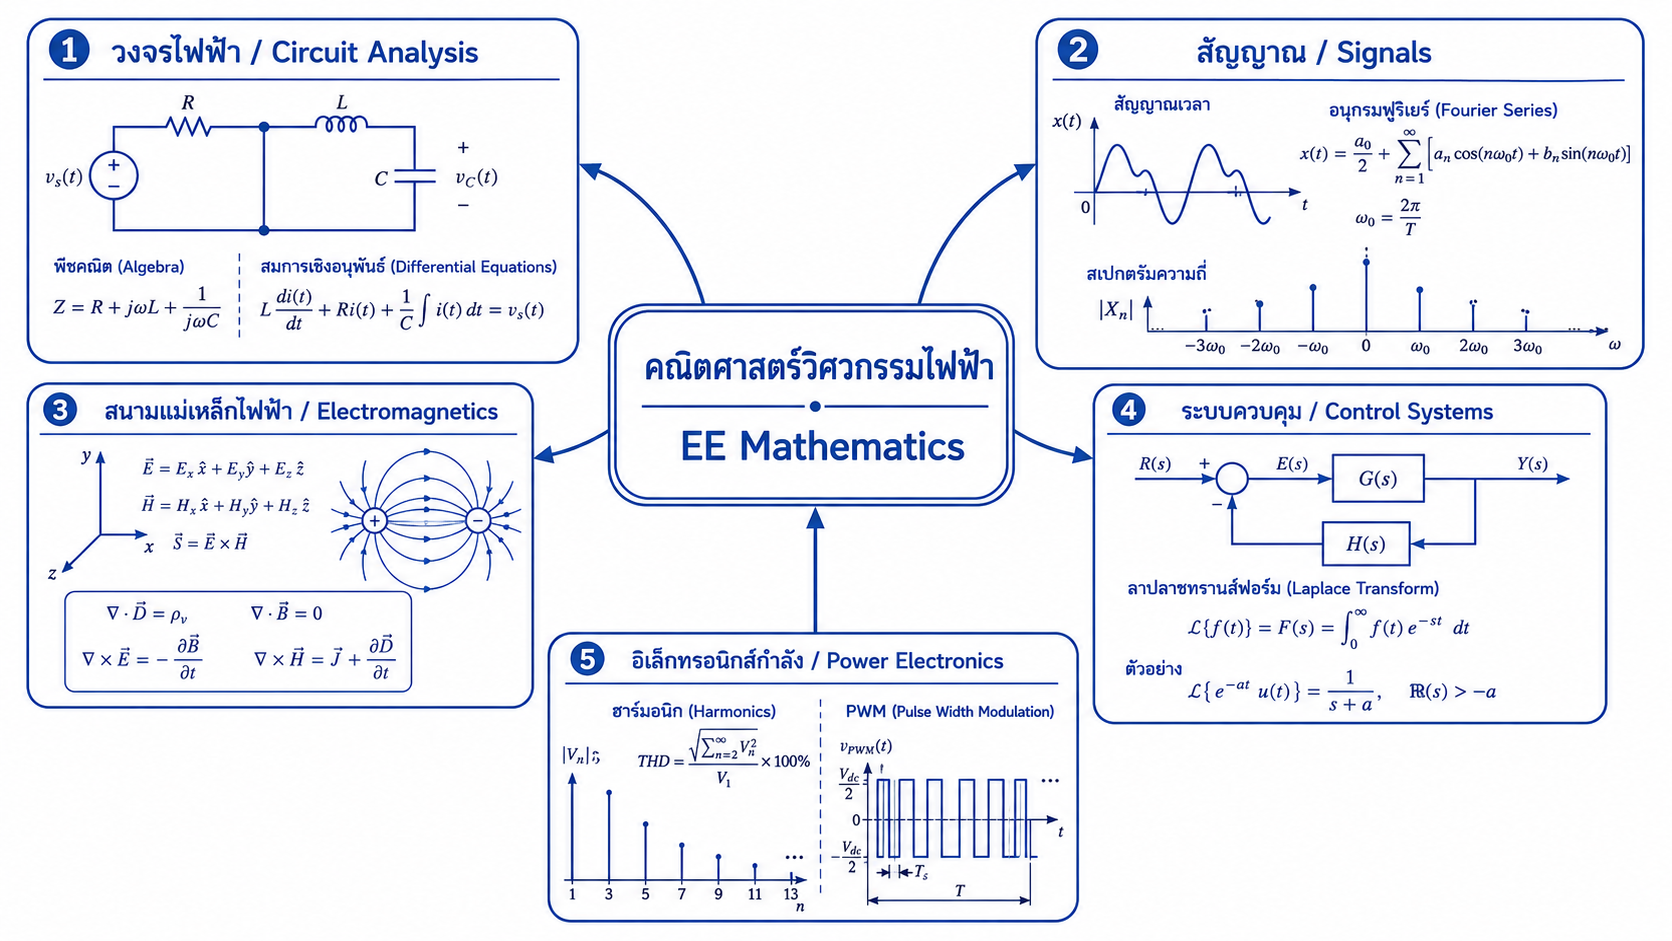
\includegraphics[width=0.8\textwidth]{images/chapter1/figure-01.png}
    \caption{แผนผังความเชื่อมโยงคณิตศาสตร์กับงานวิศวกรรมไฟฟ้า}
\end{figure}

\par\noindent\rule{\textwidth}{0.4pt}\par

\subsection{6. บทนำ}

วิศวกรรมไฟฟ้าเกี่ยวข้องกับการผลิต การส่ง การแปลง การควบคุม และการใช้พลังงานไฟฟ้า ตลอดจนการตรวจวัดและประมวลผลสัญญาณ การออกแบบระบบอิเล็กทรอนิกส์ ระบบควบคุม ระบบสื่อสาร และระบบอัตโนมัติ แม้ระบบเหล่านี้จะมีลักษณะทางกายภาพแตกต่างกัน แต่การวิเคราะห์ล้วนต้องอาศัย “แบบจำลองทางคณิตศาสตร์” เพื่อทำให้ปัญหาที่ซับซ้อนสามารถอธิบายและคำนวณได้

ตัวอย่างเช่น เมื่อพิจารณาวงจรตัวต้านทานอย่างง่าย เราใช้กฎของโอห์มเชื่อมโยงแรงดัน กระแส และความต้านทาน แต่เมื่อวงจรมีตัวเก็บประจุหรือตัวเหนี่ยวนำ ปริมาณไฟฟ้าจะเปลี่ยนแปลงตามเวลาและนำไปสู่สมการเชิงอนุพันธ์ เมื่อวิเคราะห์ไฟฟ้ากระแสสลับ สัญญาณไซน์และมุมเฟสมีบทบาทสำคัญ จึงต้องอาศัยตรีโกณมิติและจำนวนเชิงซ้อน เมื่อศึกษาสนามไฟฟ้าและสนามแม่เหล็ก จำเป็นต้องใช้เวกเตอร์และแคลคูลัสเวกเตอร์ ขณะที่การวิเคราะห์รูปคลื่นที่ไม่เป็นไซน์ต้องอาศัยอนุกรมฟูเรียร์ และการศึกษาการตอบสนองชั่วครู่ของวงจรหรือระบบควบคุมมักใช้การแปลงลาปลาซ

ดังนั้น การเรียนรายวิชานี้จึงไม่ได้มุ่งให้ผู้เรียนจดจำสูตรจำนวนมาก แต่ต้องการให้ผู้เรียนเห็น “ความสัมพันธ์ระหว่างคณิตศาสตร์กับระบบจริง” ตัวอย่างเช่น แรงดันไฟฟ้าบ้านที่ระบุเป็น 220 V ไม่ใช่ค่าสูงสุดของรูปคลื่นไซน์ แต่เป็นค่า RMS ซึ่งสัมพันธ์กับกำลังเฉลี่ยที่จ่ายให้โหลดตัวต้านทาน ความเข้าใจเช่นนี้ช่วยให้ผู้เรียนไม่เพียงคำนวณได้ แต่ยังอธิบายได้ว่าตัวเลขมีความหมายทางกายภาพอย่างไร

ในยุคที่งานวิศวกรรมใช้ซอฟต์แวร์อย่างแพร่หลาย ผู้เรียนต้องรู้ทั้งการคำนวณด้วยมือและการใช้เครื่องมือดิจิทัล การคำนวณด้วยมือทำให้เห็นโครงสร้างของปัญหา ส่วนโปรแกรมช่วยลดงานซ้ำซ้อน เพิ่มความสามารถในการสำรวจค่าพารามิเตอร์ และสร้างกราฟเพื่อมองเห็นพฤติกรรมของระบบ แต่ผลลัพธ์จากโปรแกรมต้องผ่านการตรวจสอบเสมอ โดยเฉพาะเรื่องหน่วย ลำดับขนาด เครื่องหมาย และข้อสมมติของแบบจำลอง

\par\noindent\rule{\textwidth}{0.4pt}\par

\subsection{7. เนื้อหาหลัก}

\subsubsection{7.1 ความสำคัญของคณิตศาสตร์ในงานวิศวกรรมไฟฟ้า}

\paragraph{7.1.1 คณิตศาสตร์ในฐานะภาษาของระบบไฟฟ้า}

ระบบไฟฟ้าประกอบด้วยปริมาณที่สัมพันธ์กันหลายชนิด เช่น แรงดันไฟฟ้า $V$ กระแสไฟฟ้า $I$ ความต้านทาน $R$ กำลังไฟฟ้า $P$ พลังงาน $E$ ความถี่ $f$ และมุมเฟส $\phi$ หากไม่มีสมการ การอธิบายความสัมพันธ์ของปริมาณเหล่านี้จะไม่ชัดเจนและยากต่อการตรวจสอบ

ตัวอย่างพื้นฐานที่สุดคือกฎของโอห์ม

\[
V = IR
\]

\textbf{ที่มา:} เป็นความสัมพันธ์เชิงเส้นขององค์ประกอบตัวต้านทานอุดมคติภายใต้เงื่อนไขที่ค่าความต้านทานคงที่
\textbf{ตัวแปรและหน่วย:} $V$ คือแรงดัน หน่วยโวลต์ (V), $I$ คือกระแส หน่วยแอมแปร์ (A), $R$ คือความต้านทาน หน่วยโอห์ม ($\Omega$)
\textbf{สมมติฐาน:} องค์ประกอบมีพฤติกรรมโอห์มมิกและ $R$ ไม่เปลี่ยนอย่างมีนัยสำคัญจากอุณหภูมิหรือสภาวะอื่น
\textbf{เงื่อนไขการใช้:} ใช้กับตัวต้านทานหรือช่วงการทำงานที่ความสัมพันธ์ $V$–$I$ เป็นเชิงเส้น
\textbf{ความหมายทางกายภาพ:} เมื่อ $R$ คงที่ กระแสเพิ่มตามแรงดันในสัดส่วนเดียวกัน
\textbf{ข้อจำกัด:} อุปกรณ์ไม่เชิงเส้น เช่น ไดโอด ทรานซิสเตอร์ หรือหลอดไฟบางชนิด ไม่สามารถอธิบายด้วย $V=IR$ แบบค่าคงที่เดียวได้ตลอดช่วงการทำงาน

การใช้สมการทำให้สามารถตอบคำถามเชิงวิศวกรรมได้ เช่น หากแรงดันเพิ่มขึ้น 10\% กระแสจะเปลี่ยนอย่างไร หากกำลังของโหลดสูงเกินพิกัดควรปรับความต้านทานเท่าใด หรือหากค่าที่วัดต่างจากแบบจำลอง สาเหตุอาจมาจากความคลาดเคลื่อนของอุปกรณ์หรือไม่

\paragraph{7.1.2 คณิตศาสตร์เพื่อการพยากรณ์และการออกแบบ}

บทบาทของคณิตศาสตร์ในงานวิศวกรรมสามารถแบ่งได้เป็น 4 ระดับ

\begin{enumerate}
    \item \textbf{การบรรยาย (Describe):} ใช้ตัวเลข สมการ และกราฟบอกสถานะของระบบ
    \item \textbf{การวิเคราะห์ (Analyze):} หาความสัมพันธ์ เหตุและผล หรือความไวต่อพารามิเตอร์
    \item \textbf{การพยากรณ์ (Predict):} คำนวณผลที่คาดว่าจะเกิดขึ้นเมื่ออินพุตหรือสภาวะเปลี่ยน
    \item \textbf{การออกแบบ (Design):} เลือกค่าพารามิเตอร์หรือโครงสร้างให้ระบบบรรลุข้อกำหนด
\end{enumerate}

ตัวอย่างเช่น ในวงจรแหล่งจ่ายไฟ วิศวกรอาจเริ่มจากการคำนวณกระแสโหลด ใช้สมการหากำลังสูญเสีย ประเมินอุณหภูมิ และใช้การจำลองตรวจสอบรูปคลื่น ก่อนเลือกอุปกรณ์จริง การคิดเช่นนี้แสดงว่าคณิตศาสตร์เป็นส่วนหนึ่งของวงจรการออกแบบ ไม่ใช่ขั้นตอนแยกต่างหาก

\par\noindent\rule{\textwidth}{0.4pt}\par

\subsubsection{7.2 ความสัมพันธ์ระหว่างคณิตศาสตร์กับวงจรไฟฟ้า สัญญาณ และระบบ}

คณิตศาสตร์แต่ละแขนงมีบทบาทแตกต่างกันตามลักษณะของปัญหา

\begin{table}[htbp]
    \centering
    \begin{tabular}{l l l}
        \hline
        \textbf{งานวิศวกรรมไฟฟ้า} & \textbf{เครื่องมือคณิตศาสตร์หลัก} & \textbf{ตัวอย่างการใช้งาน} \\
        \hline
        วงจรไฟฟ้ากระแสตรง & พีชคณิต สมการเชิงเส้น & หาค่าแรงดัน กระแส กำลัง และการแบ่งแรงดัน \\
        วงจรไฟฟ้ากระแสสลับ & ตรีโกณมิติ จำนวนเชิงซ้อน เฟสเซอร์ & วิเคราะห์ขนาดและมุมเฟสของแรงดัน/กระแส \\
        วงจร RC, RL, RLC ชั่วครู่ & แคลคูลัส สมการเชิงอนุพันธ์ ลาปลาซ & วิเคราะห์การชาร์จ การคายประจุ และการตอบสนองเวลา \\
        สัญญาณไฟฟ้า & ฟังก์ชัน กราฟ ฟูเรียร์ & วิเคราะห์รูปคลื่น ความถี่ และฮาร์มอนิก \\
        สนามไฟฟ้าและสนามแม่เหล็ก & เวกเตอร์ แคลคูลัสเวกเตอร์ & อธิบายขนาด ทิศทาง และการกระจายตัวของสนาม \\
        ระบบควบคุม & สมการเชิงอนุพันธ์ ลาปลาซ ฟังก์ชันถ่ายโอน & วิเคราะห์การตอบสนอง เสถียรภาพ และพฤติกรรมระบบ \\
        ระบบไฟฟ้ากำลัง & จำนวนเชิงซ้อน RMS กำลัง ฮาร์มอนิก & วิเคราะห์กำลัง คุณภาพไฟฟ้า และโหลด AC \\
        อิเล็กทรอนิกส์กำลัง & รูปคลื่น ฟูเรียร์ สมการเชิงอนุพันธ์ & วิเคราะห์ PWM อินเวอร์เตอร์ และฮาร์มอนิก \\
        \hline
    \end{tabular}
\end{table}

ความสัมพันธ์นี้เป็นเหตุผลที่รายวิชาจัดลำดับจากพื้นฐานไปสู่จำนวนเชิงซ้อน เวกเตอร์ ฟูเรียร์ และลาปลาซ ผู้เรียนควรมองแต่ละบทเป็นเครื่องมือใน “กล่องเครื่องมือทางวิศวกรรม” ที่เลือกใช้ตามประเภทของปัญหา

\par\noindent\rule{\textwidth}{0.4pt}\par

\subsubsection{7.3 ภาพรวมเนื้อหาคณิตศาสตร์ที่ใช้ในรายวิชา}

\paragraph{7.3.1 พีชคณิตและการจัดรูปสมการ}

พีชคณิตเป็นพื้นฐานของการแปลงสมการเพื่อหาตัวแปรที่ต้องการ ตัวอย่างจากกฎของโอห์ม

\[
V = IR
\]

สามารถจัดรูปเป็น

\[
I = \frac{V}{R}
\]

และ

\[
R = \frac{V}{I}
\]

การจัดรูปสมการต้องรักษาสมดุลทั้งสองข้างของสมการ ผู้เรียนควรฝึกแยกตัวแปรก่อนแทนค่า เพื่อให้เห็นโครงสร้างและลดความผิดพลาด

\paragraph{7.3.2 ตรีโกณมิติ}

ฟังก์ชันไซน์และโคไซน์ใช้บรรยายสัญญาณเป็นคาบ โดยเฉพาะแรงดันและกระแส AC รูปไซน์ ความสัมพันธ์ของมุม องศา เรเดียน ความถี่ และคาบเวลาจึงเป็นพื้นฐานสำคัญของบทที่ 2 และบทที่ 4–5

\paragraph{7.3.3 จำนวนเชิงซ้อนและเฟสเซอร์}

จำนวนเชิงซ้อนเขียนได้ในรูป

\[
z = a + jb
\]

โดย $a$ เป็นส่วนจริง $b$ เป็นส่วนจินตภาพ และในงานวิศวกรรมไฟฟ้านิยมใช้ $j=\sqrt{-1}$ เพื่อหลีกเลี่ยงความสับสนกับสัญลักษณ์กระแส $i$ จำนวนเชิงซ้อนทำให้การจัดการขนาดและมุมเฟสของสัญญาณไซน์มีประสิทธิภาพมากขึ้น และจะพัฒนาอย่างเป็นระบบในบทที่ 2

\paragraph{7.3.4 เวกเตอร์}

เวกเตอร์ใช้แทนปริมาณที่มีทั้งขนาดและทิศทาง เช่น สนามไฟฟ้า $\mathbf{E}$ หรือสนามแม่เหล็ก $\mathbf{H}$ ตัวอย่างเวกเตอร์ในพิกัดคาร์ทีเซียน

\[
\mathbf{E}=E_x\mathbf{a}_x+E_y\mathbf{a}_y+E_z\mathbf{a}_z
\]

ความหมายขององค์ประกอบและการดำเนินการเวกเตอร์จะเป็นพื้นฐานของการวิเคราะห์สนามในบทที่ 3

\paragraph{7.3.5 แคลคูลัสและสมการเชิงอนุพันธ์}

อนุพันธ์ใช้บอกอัตราการเปลี่ยนแปลง ส่วนปริพันธ์ใช้บอกผลสะสม ตัวอย่างเช่น

\[
i_C(t)=C\frac{dv_C(t)}{dt}
\]

แสดงว่ากระแสผ่านตัวเก็บประจุสัมพันธ์กับอัตราการเปลี่ยนแปลงของแรงดัน การแก้สมการเช่นนี้นำไปสู่รูปเอกซ์โพเนนเชียลและต่อยอดไปสู่การแปลงลาปลาซ

\paragraph{7.3.6 อนุกรมฟูเรียร์}

อนุกรมฟูเรียร์ช่วยแยกรูปคลื่นเป็นคาบที่ไม่ใช่ไซน์บริสุทธิ์ให้เป็นผลรวมขององค์ประกอบไซน์และโคไซน์หลายความถี่ แนวคิดนี้สำคัญต่อการวิเคราะห์ฮาร์มอนิกและคุณภาพกำลังไฟฟ้าในบทที่ 4–5

\paragraph{7.3.7 การแปลงลาปลาซ}

การแปลงลาปลาซช่วยเปลี่ยนปัญหาสมการเชิงอนุพันธ์ในโดเมนเวลาให้เป็นสมการพีชคณิตในโดเมน $s$ ทำให้การวิเคราะห์วงจรชั่วครู่และระบบเชิงเส้นสะดวกขึ้น ซึ่งจะศึกษาในบทที่ 6–7

\par\noindent\rule{\textwidth}{0.4pt}\par

\subsubsection{7.4 หน่วยและสัญลักษณ์พื้นฐานทางวิศวกรรมไฟฟ้า}

\paragraph{7.4.1 เหตุผลที่หน่วยมีความสำคัญ}

คำตอบทางวิศวกรรมที่ไม่มีหน่วยมักไม่สมบูรณ์ เพราะค่าตัวเลขเดียวกันอาจหมายถึงขนาดที่แตกต่างกันอย่างมาก เช่น 5 V, 5 mV และ 5 kV ต่างกันถึงหลายลำดับขนาด การใช้หน่วยอย่างถูกต้องจึงเป็นส่วนหนึ่งของความถูกต้องของสมการ

ตารางต่อไปนี้รวบรวมปริมาณพื้นฐานที่ใช้ในบทนี้

\begin{table}[htbp]
    \centering
    \begin{tabular}{l l l l l}
        \hline
        \textbf{ปริมาณ} & \textbf{สัญลักษณ์ที่ใช้บ่อย} & \textbf{หน่วย} & \textbf{สัญลักษณ์หน่วย} & \textbf{ความหมาย} \\
        \hline
        แรงดันไฟฟ้า & $V$, $v(t)$ & โวลต์ & V & ความต่างศักย์ระหว่างสองจุด \\
        กระแสไฟฟ้า & $I$, $i(t)$ & แอมแปร์ & A & อัตราการไหลของประจุ \\
        ความต้านทาน & $R$ & โอห์ม & $\Omega$ & คุณสมบัติที่ขัดขวางการไหลของกระแส \\
        กำลังไฟฟ้า & $P$, $p(t)$ & วัตต์ & W & อัตราการถ่ายโอนหรือใช้พลังงาน \\
        พลังงาน & $E$ หรือ $W_e$ & จูล & J & พลังงานสะสมหรือพลังงานที่ถ่ายโอน \\
        เวลา & $t$ & วินาที & s & ตัวแปรอิสระของสัญญาณตามเวลา \\
        ความถี่ & $f$ & เฮิรตซ์ & Hz & จำนวนรอบต่อวินาที \\
        คาบเวลา & $T$ & วินาที & s & เวลาครบหนึ่งรอบ \\
        ความถี่เชิงมุม & $\omega$ & เรเดียนต่อวินาที & rad/s & อัตราการเปลี่ยนแปลงมุมเฟส \\
        มุมเฟส & $\phi$ & เรเดียนหรือองศา & rad หรือ $^\circ$ & ตำแหน่งเชิงมุมเทียบกับอ้างอิง \\
        \hline
    \end{tabular}
\end{table}

\paragraph{7.4.2 คำนำหน้าหน่วยที่ใช้บ่อย}

\begin{table}[htbp]
    \centering
    \begin{tabular}{l r r l}
        \hline
        \textbf{คำนำหน้า} & \textbf{สัญลักษณ์} & \textbf{ตัวคูณ} & \textbf{ตัวอย่าง} \\
        \hline
        กิกะ & G & $10^9$ & 1 GHz = $10^9$ Hz \\
        เมกะ & M & $10^6$ & 1 M$\Omega$ = $10^6\ \Omega$ \\
        กิโล & k & $10^3$ & 1 kV = $10^3$ V \\
        มิลลิ & m & $10^{-3}$ & 1 mA = $10^{-3}$ A \\
        ไมโคร & $\mu$ & $10^{-6}$ & 1 $\mu$F = $10^{-6}$ F \\
        นาโน & n & $10^{-9}$ & 1 nF = $10^{-9}$ F \\
        พิโก & p & $10^{-12}$ & 1 pF = $10^{-12}$ F \\
        \hline
    \end{tabular}
\end{table}

\textbf{ข้อควรระวัง:} ตัวพิมพ์ใหญ่และตัวพิมพ์เล็กมีความหมายต่างกัน เช่น m คือ milli แต่ M คือ mega ต่างกัน $10^9$ เท่า จึงต้องรักษารูปแบบสัญลักษณ์อย่างเคร่งครัด

\paragraph{7.4.3 การตรวจสอบมิติของสมการ}

พิจารณาสมการกำลังของโหลดตัวต้านทาน

\[
P=VI
\]

หน่วยของขวามือคือ

\[
\mathrm{V}\cdot\mathrm{A}=\mathrm{W}
\]

ถ้าคำนวณได้ตัวเลขแต่หน่วยไม่สอดคล้องกับวัตต์ แสดงว่าขั้นตอนใดขั้นตอนหนึ่งอาจผิด การตรวจหน่วยจึงเป็นวิธีตรวจความถูกต้องที่รวดเร็ว


\par\noindent\rule{\textwidth}{0.4pt}\par

\subsubsection{7.5 การทบทวนพีชคณิต ฟังก์ชัน กราฟ และสมการพื้นฐาน}

\paragraph{7.5.1 การอ่านสัญลักษณ์ค่าคงที่และฟังก์ชันของเวลา}

ในงานไฟฟ้ามักใช้ตัวพิมพ์ใหญ่แทนค่าคงที่หรือค่าเชิงเฟสเซอร์ และตัวพิมพ์เล็กที่มี $(t)$ แทนค่าทันทีที่เปลี่ยนตามเวลา ตัวอย่างเช่น

\begin{itemize}
    \item $V$ อาจหมายถึงค่าแรงดันคงที่หรือค่า RMS ตามบริบท
    \item $v(t)$ หมายถึงแรงดันทันที ณ เวลา $t$
    \item $I$ อาจหมายถึงกระแสคงที่หรือค่า RMS
    \item $i(t)$ หมายถึงกระแสทันที
\end{itemize}

ผู้เรียนต้องอ่านนิยามของสัญลักษณ์ก่อนใช้สมการทุกครั้ง เพราะสัญลักษณ์เดียวกันอาจมีความหมายต่างกันในเอกสารคนละเล่ม

\paragraph{7.5.2 ฟังก์ชันเชิงเส้น}

รูปทั่วไป

\[
y=mx+b
\]

โดย $m$ คือความชันและ $b$ คือจุดตัดแกน $y$ ความสัมพันธ์ $V=IR$ ของตัวต้านทานที่ $R$ คงที่สามารถมองเป็นเส้นตรงในกราฟ $V$ กับ $I$ โดยความชันเท่ากับ $R$

\paragraph{7.5.3 ฟังก์ชันเอกซ์โพเนนเชียล}

ฟังก์ชันเอกซ์โพเนนเชียลปรากฏบ่อยในวงจรอันดับหนึ่ง เช่น RC และ RL รูปทั่วไปของการเปลี่ยนจากค่าเริ่มต้น $x_i$ ไปสู่ค่าปลายทาง $x_f$ คือ

\[
x(t)=x_f+(x_i-x_f)e^{-t/\tau}
\]

โดย $\tau$ คือค่าคงตัวเวลา เมื่อ $t=\tau$ ส่วนต่างจากค่าปลายทางจะลดเหลือ $e^{-1}\approx0.368$ ของค่าเริ่มต้น และเมื่อประมาณ $5\tau$ ระบบอันดับหนึ่งจะเข้าใกล้ค่าปลายทางมากกว่า 99\% ในเชิงวิศวกรรม

สำหรับวงจร RC

\[
\tau=RC
\]

\textbf{ตัวแปรและหน่วย:} $R$ หน่วยโอห์ม, $C$ หน่วยฟารัด, $\tau$ หน่วยวินาที
\textbf{สมมติฐาน:} $R$ และ $C$ คงที่ วงจรเป็นเชิงเส้น และแหล่งจ่ายเปลี่ยนแบบขั้นบันไดอุดมคติ
\textbf{ความหมายทางกายภาพ:} $\tau$ บอกความเร็วของการตอบสนอง ยิ่ง $RC$ มาก การเปลี่ยนแปลงยิ่งช้า
\textbf{ข้อจำกัด:} อุปกรณ์จริงมีความคลาดเคลื่อนและความต้านทานแฝง จึงอาจทำให้ค่าที่วัดต่างจากแบบจำลอง

% [รูปที่ 2: กราฟการชาร์จและคายประจุของวงจร RC]
% ประเภทภาพ: Graph
% ตำแหน่งที่แนะนำ: หลังหัวข้อ 7.5.3 ฟังก์ชันเอกซ์โพเนนเชียล
% วัตถุประสงค์การเรียนรู้: แสดงความหมายของค่าคงตัวเวลา $\tau$ และพฤติกรรมเข้าใกล้ค่าปลายทางแบบเอกซ์โพเนนเชียล
% คำอธิบายภาพ: แสดงกราฟ normalized voltage เทียบกับเวลา มีเส้น Charging $vC(t)=V0(1-e^{-t/\tau})$ และ Discharging $vC(t)=V0e^{-t/\tau}$ ทำเครื่องหมายที่ $t=\tau$ และ $t=5\tau$ พร้อมค่าประมาณ 0.632 และ 0.368 ที่ $t=\tau$
% องค์ประกอบที่ต้องมี: แกนเวลา $t/\tau$, แกน $vC/V0$, เส้นชาร์จ เส้นคายประจุ เส้นประที่ $\tau$ และ $5\tau$
% ข้อความหรือป้ายกำกับ: “Charging”, “Discharging”, “$t=\tau$”, “$t=5\tau$”, “0.632”, “0.368”
% ภาษาของป้ายกำกับ: อังกฤษและสัญลักษณ์ทางคณิตศาสตร์
% สัดส่วนภาพ: 16:9
% Graph Generation Prompt: Plot normalized RC charging y=1-exp(-t/tau) and discharging y=exp(-t/tau) for t from 0 to 5tau. Horizontal axis labeled t/tau, vertical axis labeled vC/V0. Mark t=tau with charging=0.632 and discharging=0.368, and mark t=5tau. Use clear engineering textbook annotations, white background, readable legend and grid.
% Alt Text: กราฟสองเส้นแสดงแรงดันตัวเก็บประจุขณะชาร์จเพิ่มจากศูนย์เข้าใกล้หนึ่ง และขณะคายประจุลดจากหนึ่งเข้าใกล้ศูนย์ โดยเน้นจุดหนึ่งค่าคงตัวเวลา

\begin{figure}[htbp]
    \centering
    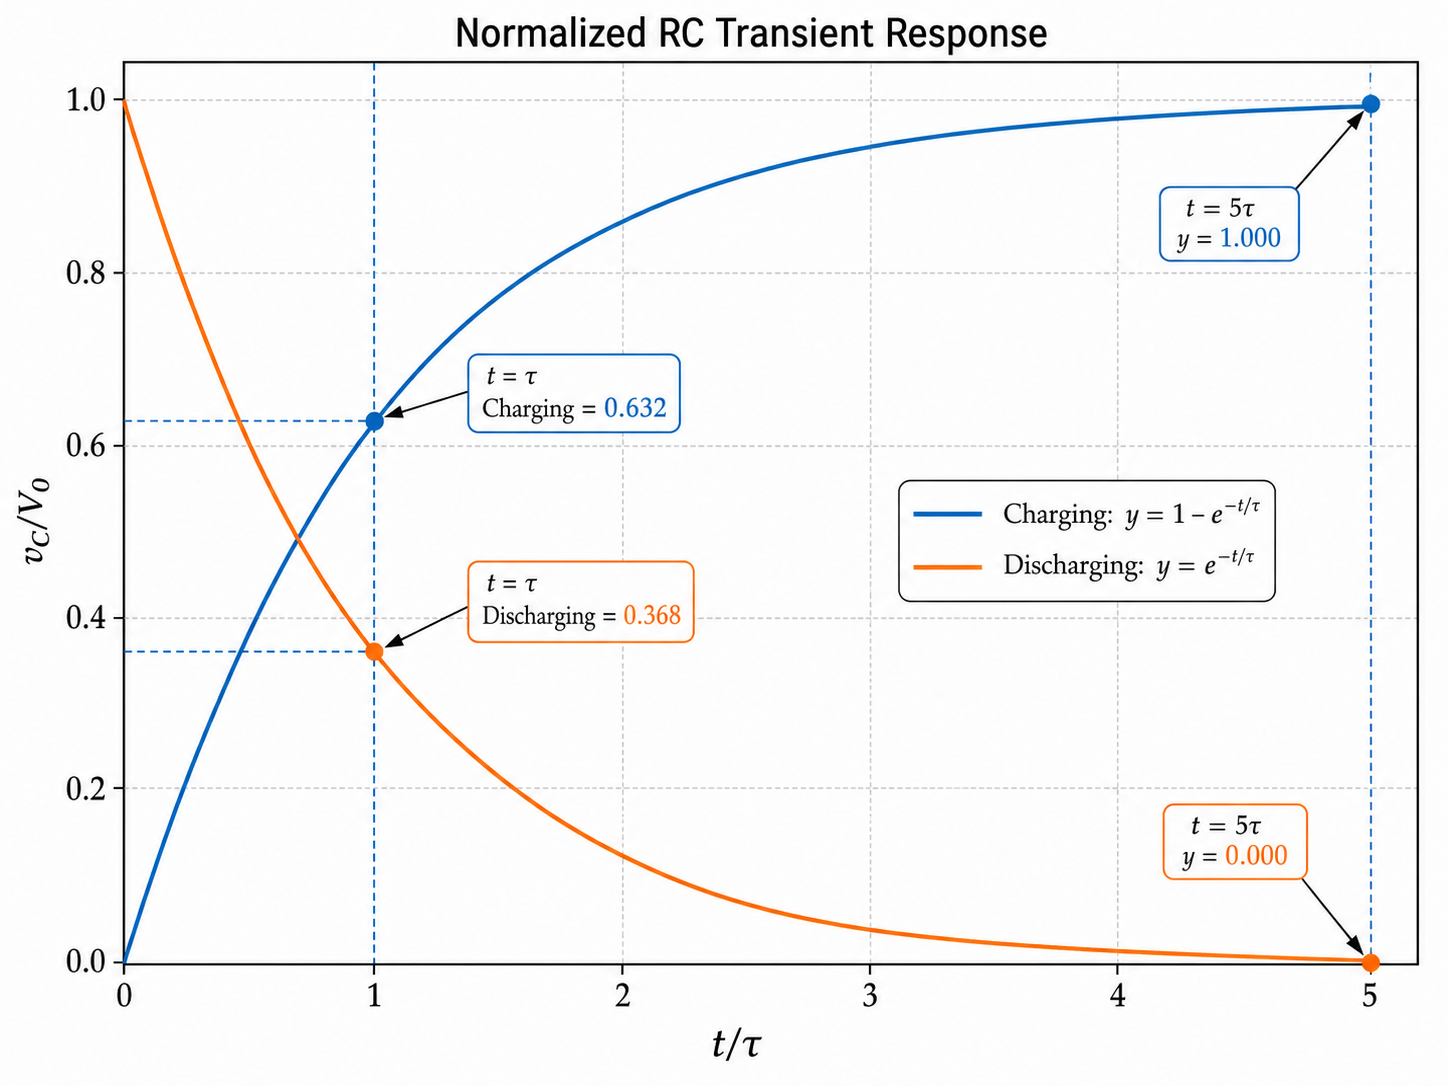
\includegraphics[width=0.8\textwidth]{images/chapter1/figure-02.png}
    \caption{กราฟการชาร์จและคายประจุของวงจร RC}
\end{figure}

\paragraph{7.5.4 ฟังก์ชันไซน์และการแทนสัญญาณ AC}

แรงดันไฟฟ้ากระแสสลับแบบไซน์เขียนได้เป็น

\[
v(t)=V_m\sin(\omega t+\phi)
\]

\textbf{ที่มา:} เป็นแบบจำลองมาตรฐานของสัญญาณฮาร์มอนิกหนึ่งความถี่
\textbf{ตัวแปรและหน่วย:}

\begin{itemize}
    \item $v(t)$ แรงดันทันที หน่วย V
    \item $V_m$ ค่าสูงสุดหรือแอมพลิจูด หน่วย V
    \item $\omega$ ความถี่เชิงมุม หน่วย rad/s
    \item $t$ เวลา หน่วย s
    \item $\phi$ มุมเฟสเริ่มต้น หน่วย rad หรือ $^\circ$
\end{itemize}

\textbf{สมมติฐาน:} สัญญาณเป็นไซน์บริสุทธิ์และพารามิเตอร์คงที่ในช่วงที่วิเคราะห์
\textbf{เงื่อนไขการใช้:} ใช้แทนแรงดันหรือกระแส AC รูปไซน์ และเป็นพื้นฐานของการวิเคราะห์แบบเฟสเซอร์
\textbf{ความหมายทางกายภาพ:} $V_m$ ควบคุมขนาด, $f$ หรือ $\omega$ ควบคุมความเร็วในการวนรอบ, $\phi$ กำหนดการเลื่อนตามแกนเวลา
\textbf{ข้อจำกัด:} รูปคลื่นจากอุปกรณ์สวิตชิ่งหรือโหลดไม่เชิงเส้นอาจไม่ใช่ไซน์บริสุทธิ์และต้องใช้การวิเคราะห์ฮาร์มอนิกเพิ่มเติม

ความสัมพันธ์ระหว่างความถี่ คาบเวลา และความถี่เชิงมุมคือ

\[
T=\frac{1}{f}
\]

และ

\[
\omega=2\pi f=\frac{2\pi}{T}
\]

\textbf{ตัวแปรและหน่วย:} $T$ หน่วย s, $f$ หน่วย Hz, $\omega$ หน่วย rad/s
\textbf{ความหมายทางกายภาพ:} หนึ่งรอบของสัญญาณเท่ากับ $2\pi$ เรเดียน ดังนั้นถ้ามี $f$ รอบต่อวินาที ความเร็วเชิงมุมคือ $2\pi f$ เรเดียนต่อวินาที

\textbf{ตัวอย่างสั้น:} ระบบ 50 Hz มี

\[
T=\frac{1}{50}=0.02\ \mathrm{s}=20\ \mathrm{ms}
\]

และ

\[
\omega=2\pi(50)\approx314.16\ \mathrm{rad/s}
\]

% [รูปที่ 3: กราฟสัญญาณไซน์แสดงพารามิเตอร์สำคัญ]
% ประเภทภาพ: Graph
% ตำแหน่งที่แนะนำ: หลังหัวข้อ 7.5.4 ฟังก์ชันไซน์และการแทนสัญญาณ AC
% วัตถุประสงค์การเรียนรู้: ช่วยให้ผู้เรียนเชื่อมสมการ $v(t)=Vm\sin(\omega t+\phi)$ กับความหมายเชิงกราฟของแอมพลิจูด คาบ และเฟส
% คำอธิบายภาพ: กราฟไซน์หนึ่งถึงสองคาบ แสดงระดับ $+Vm$ และ $-Vm$ ลูกศรค่ายอดถึงยอด $2Vm$ ช่วงคาบ $T$ และการเลื่อนเฟส $\phi$ พร้อมตำแหน่ง zero crossing ที่เหมาะสม
% องค์ประกอบที่ต้องมี: แกน $t$, แกน $v(t)$, เส้นไซน์, เส้นประ $\pm Vm$, ลูกศร $2Vm$, ลูกศร $T$, ตัวบ่งชี้ phase shift
% ข้อความหรือป้ายกำกับ: $Vm$, $-Vm$, $V{pp}=2Vm$, $T=2\pi/\omega$, $\phi$, $v(t)=Vm\sin(\omega t+\phi)$
% ภาษาของป้ายกำกับ: สัญลักษณ์คณิตศาสตร์และอังกฤษสั้น ๆ
% สัดส่วนภาพ: 16:9
% Graph Generation Prompt: Engineering textbook graph of v(t)=Vm sin(omega t + phi) over about two periods. Show horizontal time axis t and vertical voltage axis v(t), dashed levels at +Vm and -Vm, a vertical double arrow labeled Vpp=2Vm, a horizontal arrow labeled T=2pi/omega, and a phase-shift annotation phi. Mark representative zero crossings. White background, clean precise linework, readable mathematical labels, 16:9.
% Alt Text: กราฟไซน์แสดงค่าสูงสุดบวกและลบ ค่ายอดถึงยอด คาบเวลา และการเลื่อนเฟสตามสมการสัญญาณไซน์

\begin{figure}[htbp]
    \centering
    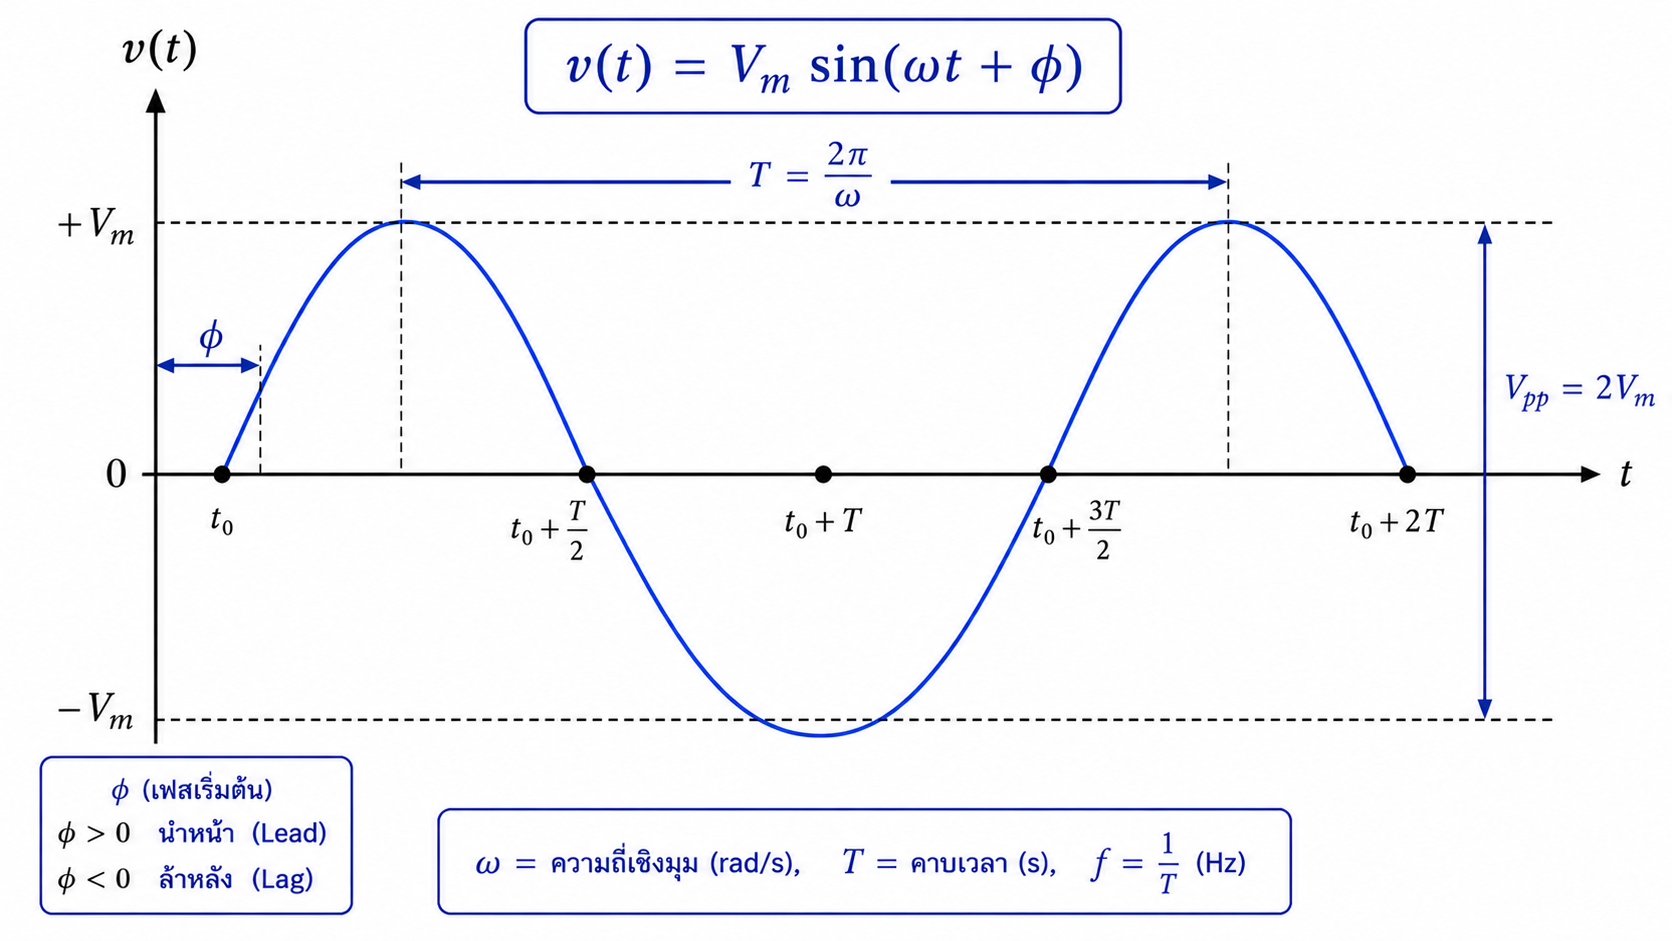
\includegraphics[width=0.8\textwidth]{images/chapter1/figure-03.png}
    \caption{กราฟสัญญาณไซน์แสดงพารามิเตอร์สำคัญ}
\end{figure}

\paragraph{7.5.5 ค่าสูงสุด ค่ายอดถึงยอด ค่าเฉลี่ย และค่า RMS}

สำหรับสัญญาณไซน์สมมาตรรอบศูนย์ ค่าสูงสุดคือ $V_m$ และค่ายอดถึงยอดคือ

\[
V_{pp}=2V_m
\]

ค่าเฉลี่ยทั่วไปของสัญญาณในช่วงหนึ่งคาบนิยามเป็น

\[
V_{\mathrm{avg}}=\frac{1}{T}\int_0^T v(t)\,dt
\]

สำหรับไซน์บริสุทธิ์ตลอดหนึ่งคาบ ค่าเฉลี่ยเท่ากับศูนย์ เพราะพื้นที่บวกและลบหักล้างกัน

\textbf{ข้อสังเกตสำคัญเรื่องค่าเฉลี่ย:} หากพิจารณาเฉพาะครึ่งคาบบวกของไซน์ ค่าเฉลี่ยบนช่วงครึ่งคาบนั้นเท่ากับ $2V_m/\pi$ แต่หากเป็น “สัญญาณครึ่งคลื่นที่ถูกเรียงกระแส” แล้วหาค่าเฉลี่ยตลอดหนึ่งคาบ ค่าเฉลี่ยเท่ากับ $V_m/\pi$ ผู้เรียนต้องระบุช่วงอินทิเกรตให้ชัดเจนเพื่อหลีกเลี่ยงความสับสน

ค่า RMS ของสัญญาณคาบนิยามเป็น

\[
V_{\mathrm{rms}}=\sqrt{\frac{1}{T}\int_0^T v^2(t)\,dt}
\]

สำหรับไซน์บริสุทธิ์

\[
V_{\mathrm{rms}}=\frac{V_m}{\sqrt{2}}\approx0.707V_m
\]

และ

\[
I_{\mathrm{rms}}=\frac{I_m}{\sqrt{2}}\approx0.707I_m
\]

\textbf{ที่มา:} นิยาม RMS มาจากการยกกำลังสอง ค่าเฉลี่ย และถอดราก เพื่อให้ได้ค่าบวกที่สัมพันธ์กับผลของกำลังในโหลดตัวต้านทาน
\textbf{สมมติฐานสำหรับสูตร $V_m/\sqrt{2}$:} รูปคลื่นต้องเป็นไซน์บริสุทธิ์
\textbf{ความหมายทางกายภาพ:} แรงดัน AC ที่มีค่า RMS เท่ากับแรงดัน DC จะให้กำลังเฉลี่ยเท่ากันบนตัวต้านทานเดียวกัน
\textbf{ข้อจำกัด:} สำหรับรูปคลื่นไม่เป็นไซน์ ห้ามใช้ $0.707V_m$ โดยอัตโนมัติ ต้องใช้คำนิยาม RMS หรือวิธีที่เหมาะกับรูปคลื่นนั้น

% [รูปที่ 4: เปรียบเทียบ Peak, Peak-to-Peak และ RMS ของสัญญาณไซน์]
% ประเภทภาพ: Graph
% ตำแหน่งที่แนะนำ: หลังหัวข้อ 7.5.5
% วัตถุประสงค์การเรียนรู้: แยกความหมายของ $Vm$, $V{pp}$ และ $V{rms}$ ซึ่งผู้เรียนมักสับสน
% คำอธิบายภาพ: กราฟไซน์หนึ่งคาบ มีเส้นประระดับ $+Vm$, $-Vm$ และ $+0.707Vm$ พร้อมลูกศรบอก $Vm$ และ $2Vm$
% องค์ประกอบที่ต้องมี: รูปคลื่นไซน์ แกน $t$, แกน $v(t)$ เส้นประ $\pm Vm$, เส้น RMS, ลูกศร $Vm$ และ $V{pp}$
% ข้อความหรือป้ายกำกับ: “Peak $Vm$”, “RMS $=0.707Vm$”, “Peak-to-Peak $=2Vm$”
% ภาษาของป้ายกำกับ: อังกฤษและสัญลักษณ์
% สัดส่วนภาพ: 16:9
% Graph Generation Prompt: Plot one period of a sinusoidal waveform centered at zero. Mark +Vm and -Vm with horizontal dashed lines, mark +0.707Vm as the positive RMS magnitude reference, show a vertical arrow from zero to +Vm labeled Peak Vm, and a vertical double arrow from -Vm to +Vm labeled Peak-to-Peak 2Vm. Include axes v(t) and t, clean engineering textbook style, white background, clear legend.
% Alt Text: กราฟไซน์หนึ่งคาบแสดงความแตกต่างระหว่างค่าสูงสุด ค่ายอดถึงยอด และค่า RMS

\begin{figure}[htbp]
    \centering
    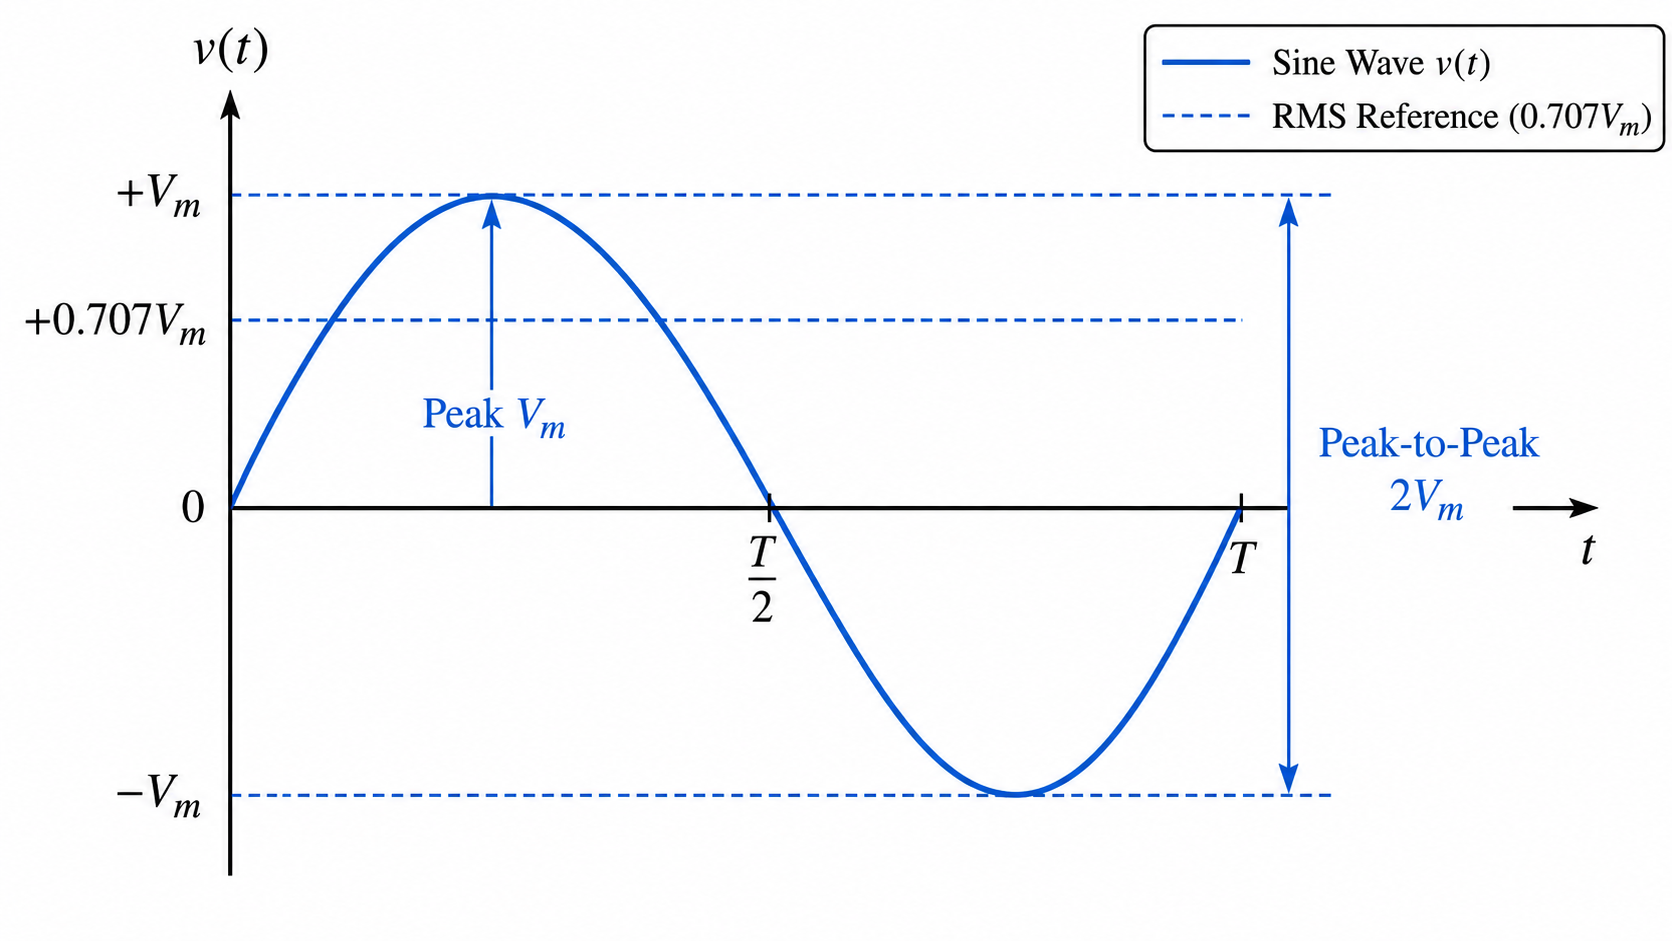
\includegraphics[width=0.8\textwidth]{images/chapter1/figure-04.png}
    \caption{เปรียบเทียบ Peak, Peak-to-Peak และ RMS ของสัญญาณไซน์}
\end{figure}

\paragraph{7.5.6 ความต่างเฟสและการเลื่อนเวลา}

หากสัญญาณสองสัญญาณมีความถี่เท่ากันแต่ต่างเฟสกัน $\Delta\phi$ ความต่างเวลาคำนวณได้จาก

\[
\Delta t=\frac{\Delta\phi}{2\pi f}
\]

เมื่อ $\Delta\phi$ อยู่ในหน่วยเรเดียน หรือ

\[
\Delta t=\left(\frac{\Delta\phi(^\circ)}{360^\circ}\right)T
\]

เมื่อมุมอยู่ในหน่วยองศา

\textbf{เงื่อนไขการใช้:} สัญญาณต้องมีความถี่เดียวกัน
\textbf{ความหมายทางกายภาพ:} มุมเฟสคือการบอกตำแหน่งในรอบ ถ้าหนึ่งรอบใช้เวลา $T$ การเหลื่อม $30^\circ$ จึงเท่ากับ $30/360$ ของคาบ
\textbf{ข้อควรระวัง:} เครื่องหมายของ $\Delta t$ ขึ้นกับนิยามว่าสัญญาณใดเป็นตัวอ้างอิงและใช้คำว่า “นำ” หรือ “ล้า”

\paragraph{7.5.7 สัญญาณรูปแบบอื่นที่ควรรู้จัก}

แม้บทนี้เน้นสัญญาณไซน์ ผู้เรียนควรรู้จักรูปคลื่นพื้นฐานอื่นเพื่อเตรียมพร้อมสำหรับบทต่อไป

\begin{itemize}
    \item \textbf{สัญญาณขั้นบันได (Unit Step):} ใช้แทนการเปลี่ยนสถานะทันที เช่น การเปิดสวิตช์
    \item \textbf{สัญญาณเอกซ์โพเนนเชียล:} พบในการตอบสนองชั่วครู่ของวงจร RC และ RL
    \item \textbf{สัญญาณสี่เหลี่ยม:} พบในวงจรดิจิทัลและ PWM มีฮาร์มอนิกหลายอันดับ
    \item \textbf{สัญญาณสามเหลี่ยมและฟันเลื่อย:} พบในการสร้างสัญญาณ การมอดูเลต และวงจรควบคุมบางประเภท
\end{itemize}

รูปคลื่นที่ไม่เป็นไซน์บริสุทธิ์จะเชื่อมโยงโดยตรงกับอนุกรมฟูเรียร์ในบทที่ 4 และการวิเคราะห์รูปคลื่นไฟฟ้าในบทที่ 5

\par\noindent\rule{\textwidth}{0.4pt}\par

\subsubsection{7.6 การคำนวณเชิงตัวเลขและการประมาณค่า}

\paragraph{7.6.1 สัญกรณ์วิทยาศาสตร์และสัญกรณ์วิศวกรรม}

การเขียนตัวเลขขนาดใหญ่มากหรือเล็กมากในรูป

\[
a\times10^n
\]

ช่วยให้คำนวณและเปรียบเทียบลำดับขนาดได้ง่าย ในสัญกรณ์วิศวกรรม มักเลือกเลขชี้กำลังเป็นพหุคูณของ 3 เพื่อให้สัมพันธ์กับคำนำหน้าหน่วย เช่น

\[
0.0000047\ \mathrm{F}=4.7\times10^{-6}\ \mathrm{F}=4.7\ \mu\mathrm{F}
\]

และ

\[
4700\ \Omega=4.7\times10^3\ \Omega=4.7\ \mathrm{k}\Omega
\]

\paragraph{7.6.2 เลขนัยสำคัญ}

เลขนัยสำคัญสะท้อนความละเอียดของข้อมูล ตัวอย่างเช่น หากตัวต้านทานระบุ $100\ \Omega$ ด้วยความคลาดเคลื่อน 5\% การรายงานผลคำนวณเป็น $99.999873\ \Omega$ ไม่มีความหมายทางกายภาพมากกว่าการรายงานอย่างเหมาะสมตามความละเอียดของข้อมูล

แนวปฏิบัติพื้นฐานคือ

\begin{itemize}
    \item เก็บจำนวนหลักมากพอในระหว่างการคำนวณ
    \item ปัดเศษในขั้นตอนสุดท้าย
    \item ไม่รายงานทศนิยมมากเกินความแม่นของข้อมูลนำเข้า
    \item ระบุหน่วยทุกครั้ง
\end{itemize}

\paragraph{7.6.3 ความคลาดเคลื่อนสัมบูรณ์และความคลาดเคลื่อนสัมพัทธ์}

ให้ $x_{ref}$ เป็นค่าอ้างอิง และ $x_{approx}$ เป็นค่าประมาณ

\[
E_{abs}=|x_{ref}-x_{approx}|
\]

ความคลาดเคลื่อนสัมพัทธ์คือ

\[
E_{rel}=\frac{|x_{ref}-x_{approx}|}{|x_{ref}|}
\]

และร้อยละความคลาดเคลื่อนคือ

\[
E_{\%}=E_{rel}\times100\%
\]

\textbf{ข้อจำกัด:} หาก $x_{ref}=0$ ไม่สามารถใช้สูตรความคลาดเคลื่อนสัมพัทธ์แบบนี้ได้โดยตรง

\paragraph{7.6.4 การประมาณค่าเพื่อทดสอบความสมเหตุสมผล}

ก่อนกดเครื่องคิดเลขควรถามว่า “คำตอบควรอยู่ประมาณเท่าใด” ตัวอย่างเช่น $220^2/100$ ควรมีค่าประมาณ $484$ ไม่ใช่ $48{,}400$ หรือ $4.84$ การประมาณลำดับขนาดช่วยจับข้อผิดพลาดเรื่องจุดทศนิยม คำนำหน้าหน่วย และการพิมพ์สูตรผิด

\textbf{ตัวอย่าง:} ถ้าโหลด $R=100\ \Omega$ ต่อกับ $V_{rms}=220\ \mathrm{V}$

\[
P=\frac{V_{rms}^2}{R}\approx\frac{(2.2\times10^2)^2}{10^2}\approx4.84\times10^2\ \mathrm{W}
\]

ดังนั้นคำตอบควรอยู่ระดับหลายร้อยวัตต์

\paragraph{7.6.5 ความผิดพลาดเชิงตัวเลขที่พบบ่อย}

\begin{enumerate}
    \item ใช้องศาแทนเรเดียนหรือกลับกัน
    \item พิมพ์วงเล็บไม่ครบ เช่น $1/2\pi f$ แทน $1/(2\pi f)$
    \item ลืมแปลง mA เป็น A ก่อนคำนวณกำลัง
    \item ปัดเศษเร็วเกินไปจนเกิดความคลาดเคลื่อนสะสม
    \item ใช้ค่าคงที่ $\pi\approx3.14$ ในขั้นตอนกลางมากเกินจำเป็น
    \item เชื่อผลเครื่องคิดเลขโดยไม่ตรวจลำดับขนาด
\end{enumerate}

\par\noindent\rule{\textwidth}{0.4pt}\par

\subsubsection{7.7 เครื่องมือคำนวณทางคณิตศาสตร์สำหรับวิศวกรรมไฟฟ้า}

เครื่องมือคำนวณช่วยให้ผู้เรียนทดลองกับปัญหาที่มีข้อมูลจำนวนมากหรือแสดงผลเป็นกราฟได้สะดวก แต่การเลือกเครื่องมือควรสัมพันธ์กับวัตถุประสงค์

\begin{table}[htbp]
    \centering
    \begin{tabular}{l l l l}
        \hline
        \textbf{เครื่องมือ} & \textbf{จุดเด่น} & \textbf{การใช้งานที่เหมาะสมในรายวิชา} & \textbf{ข้อสังเกต} \\
        \hline
        เครื่องคิดเลขวิทยาศาสตร์ & รวดเร็ว พกพา ใช้งานออฟไลน์ & คำนวณพื้นฐาน จำนวนเชิงซ้อน ตรีโกณมิติ & ต้องตรวจโหมด DEG/RAD \\
        Python & ภาษาทั่วไป ใช้งานได้กว้าง มีระบบนิเวศวิทยาศาสตร์ & คำนวณ สร้างกราฟ วิเคราะห์ข้อมูล และเขียนสคริปต์ & ต้องติดตั้งไลบรารีหรือใช้ Notebook ออนไลน์ \\
        NumPy & อาร์เรย์และการคำนวณเชิงตัวเลข & เวกเตอร์ เมทริกซ์ ฟังก์ชันตรีโกณมิติ & เน้นการคำนวณเชิงตัวเลข \\
        Matplotlib & การสร้างภาพและกราฟ & รูปคลื่นแรงดัน กระแส และผลการจำลอง & ต้องกำหนดแกน หน่วย และคำอธิบายให้ชัด \\
        SciPy & อัลกอริทึมวิทยาศาสตร์และวิศวกรรม & อินทิเกรต ระบบสัญญาณ การเพิ่มประสิทธิภาพ & เหมาะกับงานที่ซับซ้อนกว่าพื้นฐาน \\
        SymPy & คำนวณเชิงสัญลักษณ์ & จัดรูปสมการ อนุพันธ์ ปริพันธ์ และตรวจสมการ & ผลเชิงสัญลักษณ์ต้องตีความร่วมกับสมมติฐาน \\
        MATLAB & สภาพแวดล้อมคำนวณเชิงตัวเลขและกราฟสำหรับวิศวกรรม & เมทริกซ์ สัญญาณ การควบคุม และการจำลอง & สิทธิ์ใช้งานขึ้นกับสถาบัน \\
        GNU Octave & ซอฟต์แวร์เสรีที่มีไวยากรณ์ใกล้ MATLAB ในงานจำนวนมาก & งานคำนวณเมทริกซ์และกราฟพื้นฐาน & ความเข้ากันได้ไม่สมบูรณ์ทุกกรณี \\
        Google Colab & Notebook แบบโฮสต์ ใช้ผ่านเว็บโดยไม่ต้องตั้งค่าท้องถิ่น & ทดลอง Python แชร์งาน และเรียนแบบปฏิบัติ & ทรัพยากรและข้อจำกัดการใช้งานอาจเปลี่ยนแปลง \\
        GeoGebra หรือเครื่องมือกราฟออนไลน์ & สร้างกราฟแบบโต้ตอบ & สำรวจฟังก์ชันและพารามิเตอร์ & ไม่ทดแทนการคำนวณเชิงวิศวกรรมเต็มรูปแบบ \\
        \hline
    \end{tabular}
\end{table}

\paragraph{7.7.1 หลักการใช้ซอฟต์แวร์อย่างมีวิจารณญาณ}

ก่อนใช้โปรแกรม ผู้เรียนควรตอบคำถาม 5 ข้อ

\begin{enumerate}
    \item อินพุตคืออะไร และมีหน่วยอะไร
    \item สมการหรือแบบจำลองที่โปรแกรมกำลังคำนวณคืออะไร
    \item พารามิเตอร์แต่ละตัวมีช่วงค่าที่สมเหตุสมผลหรือไม่
    \item ผลลัพธ์คาดว่าจะมีลำดับขนาดประมาณใด
    \item จะตรวจสอบผลด้วยวิธีอื่นอย่างไร เช่น คำนวณด้วยมือ กรณีพิเศษ หรือการตรวจหน่วย
\end{enumerate}

\paragraph{7.7.2 ตัวอย่างโปรแกรม Python: วาดรูปคลื่นแรงดัน AC}

ตัวอย่างต่อไปใช้ NumPy สำหรับสร้างข้อมูลเวลาและคำนวณฟังก์ชันไซน์ และใช้ Matplotlib สำหรับสร้างกราฟ

\begin{verbatim}
import numpy as np
import matplotlib.pyplot as plt

# พารามิเตอร์ของสัญญาณ
Vm = 311.0          # V
f = 50.0            # Hz
omega = 2 * np.pi * f
phi = 0.0           # rad

# สร้างแกนเวลา 0–40 ms ครอบคลุม 2 คาบของระบบ 50 Hz
t = np.linspace(0.0, 0.040, 1000)

# คำนวณแรงดันตามเวลา
v = Vm * np.sin(omega * t + phi)
Vrms = Vm / np.sqrt(2)

# วาดกราฟ
plt.figure(figsize=(10, 4))
plt.plot(t * 1000, v, label="v(t)")
plt.axhline(Vm, linestyle="--", label=f"Peak = {Vm:.0f} V")
plt.axhline(Vrms, linestyle="-.", label=f"RMS = {Vrms:.1f} V")
plt.xlabel("Time (ms)")
plt.ylabel("Voltage (V)")
plt.title("Sinusoidal voltage: v(t) = 311 sin(2π50t)")
plt.grid(True)
plt.legend()
plt.tight_layout()
plt.show()
\end{verbatim}

\textbf{การอธิบายโค้ดเป็นส่วน ๆ}

\begin{itemize}
    \item \texttt{np.linspace} สร้างจุดเวลาจำนวน 1,000 จุดในช่วง 0–0.040 s
    \item \texttt{omega = 2*np.pi*f} คำนวณความถี่เชิงมุม
    \item \texttt{np.sin} คำนวณค่าไซน์แบบเวกเตอร์สำหรับทุกจุดเวลา
    \item \texttt{Vrms = Vm/np.sqrt(2)} ใช้ได้เพราะกำหนดให้สัญญาณเป็นไซน์บริสุทธิ์
    \item การคูณ \texttt{t*1000} เปลี่ยนหน่วยแกนเวลาเป็นมิลลิวินาทีเพื่ออ่านกราฟง่ายขึ้น
\end{itemize}

\textbf{ผลลัพธ์ที่ควรสังเกต:} ค่าสูงสุดประมาณ 311 V, คาบประมาณ 20 ms และค่า RMS ประมาณ 219.9 V

\textbf{การตรวจสอบผล:} คำนวณด้วยมือว่า $T=1/50=20$ ms และ $311/\sqrt{2}\approx219.9$ V แล้วเปรียบเทียบกับกราฟ

% [รูปที่ 5: ผลลัพธ์กราฟแรงดัน AC จากโปรแกรม Python/Matplotlib]
% ประเภทภาพ: Graph
% ตำแหน่งที่แนะนำ: หลังตัวอย่างโปรแกรม Python ในหัวข้อ 7.7.2
% วัตถุประสงค์การเรียนรู้: เชื่อมโค้ดกับผลลัพธ์ทางกายภาพของสัญญาณ 50 Hz
% คำอธิบายภาพ: กราฟ $v(t)=311\sin(2\pi50t)$ ตั้งแต่ 0 ถึง 40 ms แสดงสองคาบ มีเส้นอ้างอิง Peak 311 V และ RMS ประมาณ 220 V
% องค์ประกอบที่ต้องมี: แกนเวลา ms แกนแรงดัน V รูปคลื่นไซน์ เส้น Peak เส้น RMS legend และ grid
% ข้อความหรือป้ายกำกับ: “Peak = 311 V”, “RMS ≈ 220 V”, “T = 20 ms”
% ภาษาของป้ายกำกับ: อังกฤษหรือไทยและอังกฤษ
% สัดส่วนภาพ: 16:9
% Graph Generation Prompt: Plot v(t)=311sin(2pi50t) for t from 0 to 0.04 seconds, display time in milliseconds and voltage in volts. Show two periods, add horizontal reference lines for Peak=311 V and RMS=311/sqrt(2)≈220 V, and annotate T=20 ms. Include title, axes with units, legend, and grid. Clean engineering textbook graph.
% Alt Text: กราฟแรงดันไซน์ 50 เฮิรตซ์สองคาบ แสดงค่าสูงสุด 311 โวลต์ ค่า RMS ประมาณ 220 โวลต์ และคาบ 20 มิลลิวินาที

\begin{figure}[htbp]
    \centering
    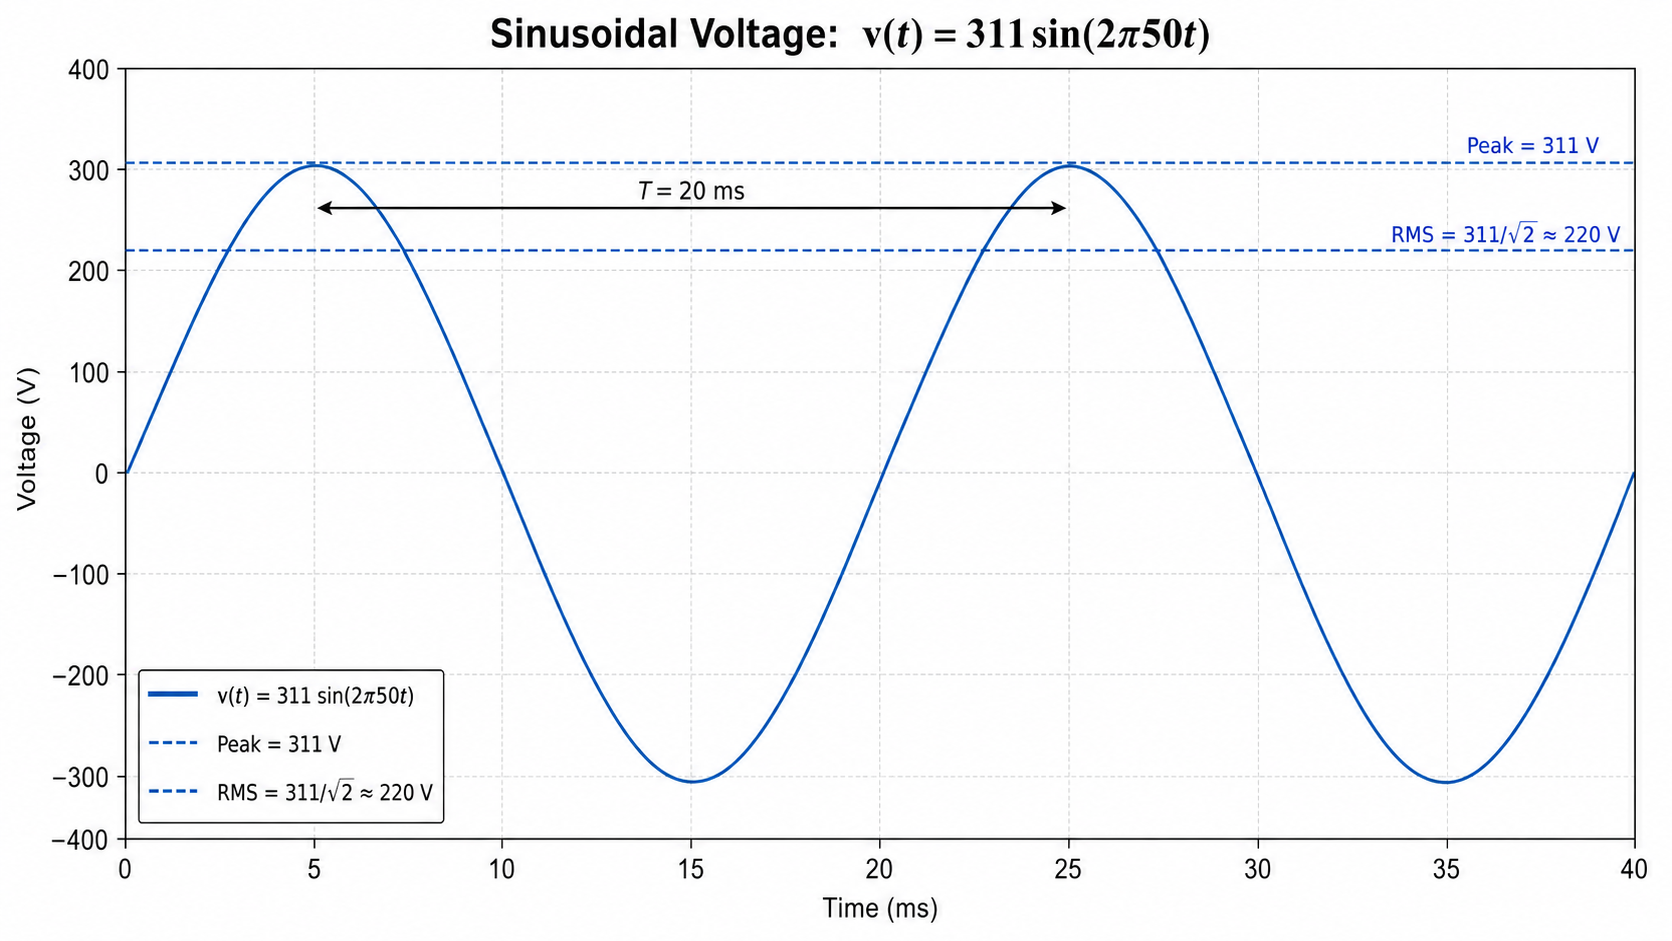
\includegraphics[width=0.8\textwidth]{images/chapter1/figure-05.png}
    \caption{ผลลัพธ์กราฟแรงดัน AC จากโปรแกรม Python/Matplotlib}
\end{figure}

\par\noindent\rule{\textwidth}{0.4pt}\par

\subsubsection{7.8 แนวทางการแก้ปัญหาทางคณิตศาสตร์ในงานวิศวกรรมไฟฟ้า}

การแก้โจทย์อย่างเป็นระบบสำคัญกว่าการจำสูตร กระบวนการแนะนำมี 9 ขั้นตอน

\paragraph{ขั้นที่ 1 ทำความเข้าใจระบบและคำถาม}

ระบุว่าโจทย์ต้องการหาอะไร ระบบเป็น DC หรือ AC สัญญาณคงที่หรือเปลี่ยนตามเวลา และมีองค์ประกอบใดบ้าง

\paragraph{ขั้นที่ 2 กำหนดตัวแปร อ้างอิง และหน่วย}

เขียนสัญลักษณ์ของค่าที่ทราบและค่าที่ไม่ทราบ แปลงหน่วยให้อยู่ในระบบที่สอดคล้องกัน เช่น mA เป็น A ก่อนแทนในสูตรกำลัง

\paragraph{ขั้นที่ 3 วาดภาพหรือแบบจำลองอย่างง่าย}

วงจร แผนภาพบล็อก หรือกราฟช่วยลดความคลุมเครือ โดยเฉพาะเรื่องทิศทางกระแส ขั้วแรงดัน และการนำ–ล้าของเฟส

\paragraph{ขั้นที่ 4 เลือกหลักการหรือกฎ}

เลือกกฎของโอห์ม กำลังไฟฟ้า สมการไซน์ ความสัมพันธ์ $f$–$T$–$\omega$ หรือหลักการอื่นให้ตรงกับปัญหา

\paragraph{ขั้นที่ 5 สร้างสมการก่อนแทนค่า}

เขียนสมการเชิงสัญลักษณ์เพื่อเห็นความสัมพันธ์ จากนั้นจัดรูปให้ตัวแปรที่ต้องการอยู่ด้านเดียว

\paragraph{ขั้นที่ 6 แทนค่าและคำนวณ}

แทนค่าพร้อมหน่วย ควบคุมวงเล็บและโหมดเครื่องคิดเลขให้ถูกต้อง

\paragraph{ขั้นที่ 7 ตรวจสอบหน่วยและมิติ}

ตรวจว่าหน่วยสุดท้ายตรงกับปริมาณที่ต้องการ เช่น กำลังต้องเป็นวัตต์

\paragraph{ขั้นที่ 8 ตรวจสอบความสมเหตุสมผล}

ถามว่าคำตอบมีเครื่องหมายและลำดับขนาดสมเหตุสมผลหรือไม่ ถ้าแรงดันเพิ่มแต่ผลคำนวณกระแสลดทั้งที่ $R$ คงที่ อาจมีข้อผิดพลาด

\paragraph{ขั้นที่ 9 แปลความหมายทางวิศวกรรม}

คำตอบไม่ควรจบเพียงตัวเลข แต่ควรบอกว่าผลนั้นหมายถึงอะไร เช่น โหลดใช้กำลัง 484 W หรือสัญญาณที่สองนำสัญญาณแรก 1.67 ms

% [รูปที่ 6: กระบวนการแก้ปัญหาคณิตศาสตร์สำหรับงานวิศวกรรมไฟฟ้า]
% ประเภทภาพ: Flowchart
% ตำแหน่งที่แนะนำ: หลังหัวข้อ 7.8
% วัตถุประสงค์การเรียนรู้: ทำให้ผู้เรียนมีขั้นตอนมาตรฐานในการแก้ปัญหาและตรวจสอบคำตอบ
% คำอธิบายภาพ: Flowchart จาก “Understand Problem” → “Define Variables & Units” → “Draw Model” → “Select Principle” → “Form Equation” → “Substitute & Calculate” → “Check Units” → “Check Reasonableness” → “Interpret Engineering Meaning” และมีลูกศรย้อนกลับจากขั้นตรวจสอบหากผลไม่สมเหตุสมผล
% องค์ประกอบที่ต้องมี: กล่อง 9 ขั้น ลูกศรตามลำดับ ลูกศร feedback จาก Check ไปยัง Select Principle/Form Equation
% ข้อความหรือป้ายกำกับ: ไทยและอังกฤษแบบสั้น
% ภาษาของป้ายกำกับ: ไทยและอังกฤษ
% สัดส่วนภาพ: 16:9
% Image Generation Prompt: Clean engineering education flowchart with nine steps: Understand Problem → Define Variables & Units → Draw Model → Select Principle → Form Equation → Substitute & Calculate → Check Units → Check Reasonableness → Interpret Engineering Meaning. Add feedback arrows from both checking steps back to model/equation selection when an inconsistency is found. White background, precise arrows, minimal blue technical style, bilingual Thai-English labels, 16:9.
% Alt Text: ผังงานเก้าขั้นตอนสำหรับแก้ปัญหาทางวิศวกรรม ตั้งแต่ทำความเข้าใจโจทย์จนถึงแปลความหมายคำตอบ พร้อมวงรอบย้อนกลับเมื่อตรวจพบความไม่สอดคล้อง

\begin{figure}[htbp]
    \centering
    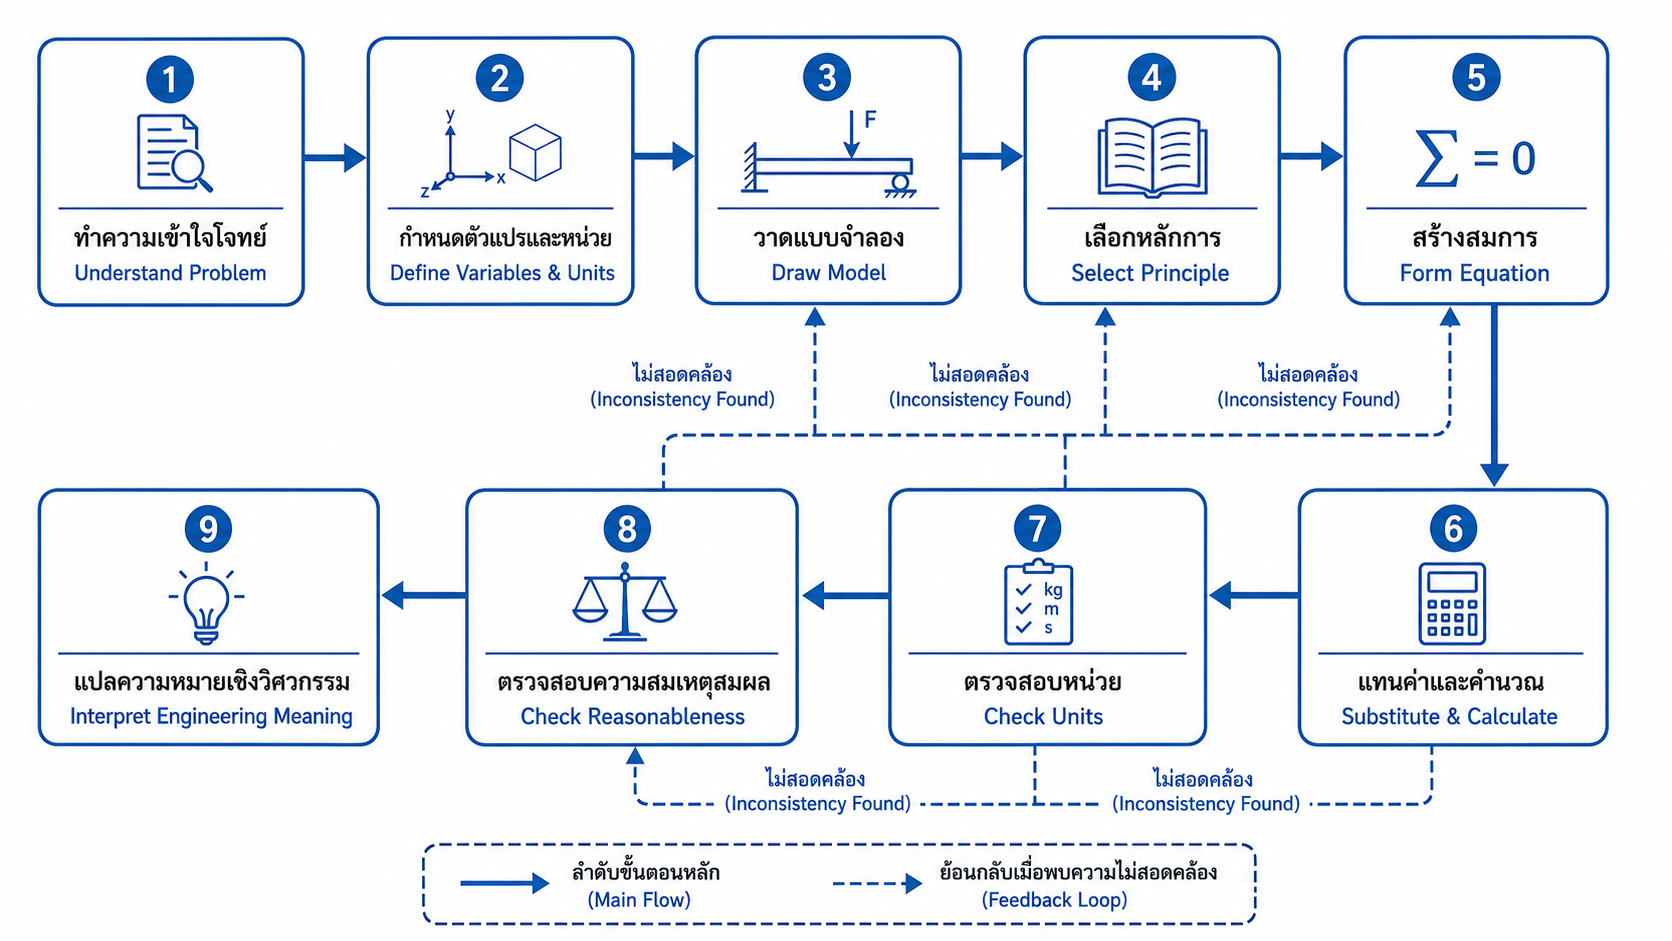
\includegraphics[width=0.8\textwidth]{images/chapter1/figure-06.png}
    \caption{กระบวนการแก้ปัญหาคณิตศาสตร์สำหรับงานวิศวกรรมไฟฟ้า}
\end{figure}


\par\noindent\rule{\textwidth}{0.4pt}\par

\subsubsection{7.9 ตัวอย่างโจทย์พื้นฐานที่เชื่อมโยงกับวงจรไฟฟ้า}

\paragraph{ตัวอย่างที่ 1.1 การใช้กฎของโอห์มและการตรวจหน่วย}

\textbf{โจทย์:} ตัวต้านทาน $R=47\ \Omega$ ต่อกับแหล่งจ่าย DC $V=12\ \mathrm{V}$ จงหากระแสที่ไหลและกำลังที่ตัวต้านทาน

\textbf{1) วิเคราะห์ระบบหรือโจทย์}
เป็นวงจร DC ตัวต้านทานอุดมคติ ต้องการ $I$ และ $P$

\textbf{2) กำหนดตัวแปรและหน่วย}
$V=12\ \mathrm{V}$, $R=47\ \Omega$

\textbf{3) เลือกกฎหรือหลักการ}
ใช้กฎของโอห์มและสูตรกำลัง

\[
I=\frac{V}{R}
\]

\[
P=VI
\]

\textbf{4) แทนค่าและคำนวณ}

\[
I=\frac{12}{47}=0.2553\ \mathrm{A}
\]

ประมาณ

\[
I\approx0.255\ \mathrm{A}=255\ \mathrm{mA}
\]

กำลัง

\[
P=(12)(0.2553)\approx3.06\ \mathrm{W}
\]

\textbf{5) ตรวจสอบหน่วย}
$\mathrm{V}/\Omega=\mathrm{A}$ และ $\mathrm{V}\cdot\mathrm{A}=\mathrm{W}$ ถูกต้อง

\textbf{6) ตรวจสอบความสมเหตุสมผล}
$12/50\approx0.24$ A ดังนั้น 0.255 A สมเหตุสมผล

\textbf{7) แปลความหมาย}
ตัวต้านทานต้องรับกำลังประมาณ 3.06 W ในแบบจำลองอุดมคติ การเลือกตัวต้านทานจริงต้องพิจารณาพิกัดกำลังและการระบายความร้อนเพิ่มเติม

\par\noindent\rule{\textwidth}{0.4pt}\par

\paragraph{ตัวอย่างที่ 1.2 การคำนวณพารามิเตอร์ของแรงดัน AC}

\textbf{โจทย์:} กำหนด

\[
v(t)=311\sin(314t)\ \mathrm{V}
\]

จงหา (ก) ค่าสูงสุด (ข) ค่า RMS (ค) ความถี่ (ง) คาบเวลา

\textbf{1) วิเคราะห์รูปมาตรฐาน}

เปรียบเทียบกับ

\[
v(t)=V_m\sin(\omega t+\phi)
\]

ได้ $V_m=311$ V, $\omega=314$ rad/s และ $\phi=0$

\textbf{2) ค่าสูงสุด}

\[
V_m=311\ \mathrm{V}
\]

\textbf{3) ค่า RMS}

\[
V_{rms}=\frac{311}{\sqrt{2}}\approx219.9\ \mathrm{V}
\]

\textbf{4) ความถี่}

\[
f=\frac{\omega}{2\pi}=\frac{314}{2\pi}\approx49.97\ \mathrm{Hz}
\]

โดยมักประมาณเป็น 50 Hz

\textbf{5) คาบเวลา}

\[
T=\frac{1}{f}\approx\frac{1}{49.97}\approx0.0200\ \mathrm{s}=20.0\ \mathrm{ms}
\]

\textbf{6) ตรวจสอบ}
ถ้า $f\approx50$ Hz คาบควรประมาณ 20 ms จึงสอดคล้องกัน

\textbf{คำตอบ:} $V_m=311$ V, $V_{rms}\approx219.9$ V, $f\approx50$ Hz และ $T\approx20$ ms

\par\noindent\rule{\textwidth}{0.4pt}\par

\paragraph{ตัวอย่างที่ 1.3 การหาสมการแรงดันจากค่า RMS}

\textbf{โจทย์:} ระบบ AC มี $V_{rms}=220\ \mathrm{V}$, $f=50\ \mathrm{Hz}$ และ $\phi=0$ จงเขียนสมการ $v(t)$ สำหรับรูปคลื่นไซน์บริสุทธิ์

\textbf{1) หาค่าสูงสุด}

\[
V_m=\sqrt{2}V_{rms}=220\sqrt{2}\approx311.13\ \mathrm{V}
\]

\textbf{2) หาความถี่เชิงมุม}

\[
\omega=2\pi f=2\pi(50)\approx314.16\ \mathrm{rad/s}
\]

\textbf{3) สร้างสมการ}

\[
v(t)=311.13\sin(314.16t)\ \mathrm{V}
\]

หรือเมื่อปัดอย่างเหมาะสม

\[
v(t)\approx311\sin(314t)\ \mathrm{V}
\]

\textbf{ตรวจสอบ:} $311.13/\sqrt{2}\approx220$ V ถูกต้อง

\textbf{ความหมาย:} ค่า 220 V เป็นค่า RMS ไม่ใช่ค่าสูงสุดของรูปคลื่น

\par\noindent\rule{\textwidth}{0.4pt}\par

\paragraph{ตัวอย่างที่ 1.4 การคำนวณกำลังเฉลี่ยในโหลดตัวต้านทาน}

\textbf{โจทย์:} แรงดัน $v(t)=311\sin(314t)$ V จ่ายให้โหลดตัวต้านทาน $R=100\ \Omega$ จงหากำลังเฉลี่ย

\textbf{1) สมมติฐาน}
โหลดเป็นตัวต้านทานล้วน และสัญญาณเป็นไซน์บริสุทธิ์

\textbf{2) หา RMS}

\[
V_{rms}=\frac{311}{\sqrt{2}}\approx219.9\ \mathrm{V}
\]

\textbf{3) เลือกสูตรกำลังสำหรับตัวต้านทาน}

\[
P=\frac{V_{rms}^2}{R}
\]

\textbf{4) แทนค่า}

\[
P=\frac{(219.9)^2}{100}\approx483.6\ \mathrm{W}
\]

หากใช้ $V_{rms}\approx220$ V จะได้ประมาณ 484 W

\textbf{5) ตรวจหน่วยและความสมเหตุสมผล}
$V^2/\Omega=W$ และค่าประมาณ 484 W สอดคล้องกับการประมาณ $220^2/100$

\textbf{คำตอบ:} โหลดได้รับกำลังเฉลี่ยประมาณ 484 W

\textbf{ข้อจำกัด:} สูตรนี้ไม่ควรถูกนำไปใช้กับโหลดที่มีรีแอกแตนซ์โดยไม่พิจารณาตัวประกอบกำลัง

\par\noindent\rule{\textwidth}{0.4pt}\par

\paragraph{ตัวอย่างที่ 1.5 การเปรียบเทียบสัญญาณต่างเฟส}

\textbf{โจทย์:}

\[
v_1(t)=100\sin(2\pi50t)
\]

และ

\[
v_2(t)=100\sin(2\pi50t+30^\circ)
\]

จงหาว่า $v_2$ นำ $v_1$ เป็นเวลาเท่าใด

\textbf{1) วิเคราะห์}
ทั้งสองสัญญาณมีความถี่ 50 Hz และต่างเฟส 30°

\textbf{2) หาคาบ}

\[
T=\frac{1}{50}=0.02\ \mathrm{s}
\]

\textbf{3) แปลงมุมเฟสเป็นเวลา}

\[
\Delta t=\left(\frac{30^\circ}{360^\circ}\right)(0.02)
\]

\[
\Delta t=0.001667\ \mathrm{s}\approx1.67\ \mathrm{ms}
\]

\textbf{4) แปลความหมาย}
เนื่องจาก $v_2$ มีเฟสบวก 30° เมื่อเทียบกับ $v_1$ ในรูปสมการนี้ จึงกล่าวว่า $v_2$ นำ $v_1$ อยู่ 30° หรือประมาณ 1.67 ms

\par\noindent\rule{\textwidth}{0.4pt}\par

\paragraph{ตัวอย่างที่ 1.6 \textbf{ตัวอย่างเพิ่มเติมเพื่อการเรียนรู้:} การคำนวณค่าคงตัวเวลา RC}

\textbf{โจทย์:} วงจร RC มี $R=10\ \mathrm{k}\Omega$ และ $C=100\ \mu\mathrm{F}$ จงหา $\tau$ และประมาณเวลาที่แรงดันตัวเก็บประจุขณะชาร์จถึงประมาณ 99\% ของค่าปลายทาง

\textbf{1) แปลงหน่วย}

\[
R=10\times10^3\ \Omega
\]

\[
C=100\times10^{-6}\ \mathrm{F}
\]

\textbf{2) ใช้สมการค่าคงตัวเวลา}

\[
\tau=RC
\]

\[
\tau=(10\times10^3)(100\times10^{-6})=1\ \mathrm{s}
\]

\textbf{3) ประมาณเวลาเข้าสู่ค่าปลายทาง}
สำหรับวงจรอันดับหนึ่ง มักใช้ $5\tau$ เป็นเกณฑ์ประมาณว่าเข้าใกล้ค่าปลายทางมากกว่า 99\%

\[
5\tau=5\ \mathrm{s}
\]

\textbf{4) แปลความหมาย}
วงจรนี้ตอบสนองค่อนข้างช้าเมื่อเทียบกับวงจรที่มี $RC$ เล็กกว่า และค่าประมาณ 5 s เป็นเกณฑ์ทางวิศวกรรม ไม่ได้หมายความว่าแรงดันเท่าค่าปลายทางอย่างสมบูรณ์

\par\noindent\rule{\textwidth}{0.4pt}\par

\subsubsection{7.10 การเชื่อมโยงกับบทต่อไป}

บทนี้เตรียมพื้นฐานให้ผู้เรียนใช้เครื่องมือที่ซับซ้อนขึ้น ดังนี้

\begin{enumerate}
    \item \textbf{บทที่ 2 จำนวนเชิงซ้อน ฟังก์ชันตัวแปรเชิงซ้อน และเฟสเซอร์}  
\end{enumerate}
   พัฒนาจากสัญญาณไซน์และมุมเฟสสู่การแทนด้วยจำนวนเชิงซ้อน ช่วยให้การวิเคราะห์ AC ลดรูปจากสมการตรีโกณมิติเป็นพีชคณิตเชิงซ้อน

\begin{enumerate}
    \item \textbf{บทที่ 3 การวิเคราะห์เวกเตอร์}  
\end{enumerate}
   พัฒนาจากแนวคิดปริมาณและหน่วยไปสู่ปริมาณที่มีทั้งขนาดและทิศทาง เพื่อใช้กับสนามไฟฟ้าและสนามแม่เหล็ก

\begin{enumerate}
    \item \textbf{บทที่ 4–5 อนุกรมฟูเรียร์และการวิเคราะห์รูปคลื่น}  
\end{enumerate}
   พัฒนาจากการรู้จักสัญญาณไซน์ สี่เหลี่ยม และสัญญาณเป็นคาบ ไปสู่การแยกองค์ประกอบความถี่และฮาร์มอนิก

\begin{enumerate}
    \item \textbf{บทที่ 6–7 การแปลงลาปลาซและการประยุกต์กับวงจร}  
\end{enumerate}
   พัฒนาจากฟังก์ชันเอกซ์โพเนนเชียลและสมการเชิงอนุพันธ์ ไปสู่การวิเคราะห์ในโดเมน $s$

\begin{enumerate}
    \item \textbf{บทที่ 8 โปรแกรมคำนวณทางคณิตศาสตร์สำหรับวิศวกรรมไฟฟ้า}  
\end{enumerate}
   ขยายจากตัวอย่าง Python เบื้องต้นในบทนี้ไปสู่การคำนวณจำนวนเชิงซ้อน เวกเตอร์ ฟูเรียร์ ลาปลาซ และการจัดทำรายงานผลอย่างเป็นระบบ

\par\noindent\rule{\textwidth}{0.4pt}\par

\subsection{8. ความเข้าใจผิดที่พบบ่อย}

\subsubsection{8.1 “แรงดันไฟฟ้าบ้าน 220 V คือค่าสูงสุด 220 V”}

\textbf{ความเข้าใจที่ถูกต้อง:} สำหรับระบบที่ระบุ 220 V AC โดยทั่วไปค่าดังกล่าวหมายถึงค่า RMS ค่าสูงสุดของไซน์บริสุทธิ์จะประมาณ $220\sqrt{2}\approx311$ V

\subsubsection{8.2 “ค่า RMS เท่ากับ 0.707 เท่าของค่าสูงสุดเสมอ”}

\textbf{ความเข้าใจที่ถูกต้อง:} ความสัมพันธ์ $V_{rms}=V_m/\sqrt{2}$ ใช้กับไซน์บริสุทธิ์เท่านั้น รูปคลื่นสี่เหลี่ยมหรือรูปคลื่นบิดเบือนมีความสัมพันธ์ต่างออกไป

\subsubsection{8.3 “ถ้าโปรแกรมให้คำตอบ แสดงว่าคำตอบถูกต้อง”}

\textbf{ความเข้าใจที่ถูกต้อง:} โปรแกรมคำนวณตามอินพุตและสมการที่ผู้ใช้กำหนด หากหน่วยผิด สูตรผิด หรือใช้แบบจำลองไม่เหมาะสม โปรแกรมอาจให้คำตอบที่ดูแม่นยำแต่ผิดทางวิศวกรรม

\subsubsection{8.4 “องศาและเรเดียนใช้แทนกันได้โดยตรง”}

\textbf{ความเข้าใจที่ถูกต้อง:} ต้องแปลงหน่วยมุมให้สอดคล้องกับฟังก์ชันหรือโหมดเครื่องคิดเลข เช่น $180^\circ=\pi$ rad

\subsubsection{8.5 “การมีทศนิยมหลายหลักหมายถึงความแม่นยำสูง”}

\textbf{ความเข้าใจที่ถูกต้อง:} จำนวนหลักที่แสดงไม่ควรเกินความละเอียดของข้อมูลและแบบจำลอง การรายงาน 6 หลักหลังจุดทศนิยมจากตัวต้านทานคลาดเคลื่อน 5\% ไม่เพิ่มความน่าเชื่อถือทางกายภาพ

\subsubsection{8.6 “ค่าเฉลี่ยของไซน์เป็น $2V_m/\pi$ เสมอ”}

\textbf{ความเข้าใจที่ถูกต้อง:} ค่าเฉลี่ยของไซน์เต็มคาบเท่ากับศูนย์ ค่า $2V_m/\pi$ เป็นค่าเฉลี่ยของไซน์บนครึ่งคาบบวก หรือเทียบเท่าค่าเฉลี่ยของไซน์ที่เรียงกระแสเต็มคลื่น ส่วนครึ่งคลื่นเรียงกระแสที่เฉลี่ยตลอดหนึ่งคาบมีค่า $V_m/\pi$

\subsubsection{8.7 “ใช้ $P=V^2/R$ ได้กับโหลด AC ทุกชนิด”}

\textbf{ความเข้าใจที่ถูกต้อง:} หากใช้ $V_{rms}^2/R$ ต้องเป็นโหลดตัวต้านทานล้วนหรือกำลังที่เกิดในส่วนต้านทาน เมื่อมีตัวเหนี่ยวนำหรือตัวเก็บประจุ ต้องพิจารณาอิมพีแดนซ์และตัวประกอบกำลังในบทที่เกี่ยวข้อง

\par\noindent\rule{\textwidth}{0.4pt}\par

\subsection{9. การประยุกต์ใช้ในงานจริง}

\subsubsection{9.1 การวิเคราะห์วงจรและเลือกพิกัดอุปกรณ์}

พีชคณิตและการตรวจหน่วยช่วยคำนวณกระแส กำลัง และพลังงาน เพื่อประเมินว่าอุปกรณ์ทำงานภายในพิกัดหรือไม่ แม้การเลือกอุปกรณ์จริงต้องพิจารณาอุณหภูมิ ความคลาดเคลื่อน และมาตรฐานความปลอดภัยเพิ่มเติม แต่การคำนวณพื้นฐานเป็นจุดเริ่มต้นของทุกขั้นตอน

\subsubsection{9.2 การอ่านค่าจากมัลติมิเตอร์และออสซิลโลสโคป}

มัลติมิเตอร์ AC มักรายงานค่า RMS ตามคุณสมบัติของเครื่องมือ ขณะที่ออสซิลโลสโคปแสดงรูปคลื่นตามเวลา ผู้ใช้จึงต้องแยกความหมายระหว่างค่าสูงสุด ค่ายอดถึงยอด และ RMS การนำค่าจากเครื่องมือคนละชนิดมาเปรียบเทียบต้องตรวจว่ากำลังวัดปริมาณเดียวกันหรือไม่

\subsubsection{9.3 การวิเคราะห์คุณภาพรูปคลื่น}

อินเวอร์เตอร์ แหล่งจ่ายไฟสวิตชิ่ง และไดรฟ์มอเตอร์สร้างรูปคลื่นที่อาจไม่เป็นไซน์บริสุทธิ์ การมองกราฟช่วยระบุการบิดเบือนเบื้องต้น แต่การวิเคราะห์เชิงความถี่ต้องใช้อนุกรมฟูเรียร์และสเปกตรัม

\subsubsection{9.4 ระบบควบคุมและการตอบสนองชั่วครู่}

สัญญาณขั้นบันไดเป็นแบบจำลองของการเปลี่ยนคำสั่งทันที เช่น เปลี่ยนค่าความเร็วอ้างอิง ส่วนการตอบสนองเอกซ์โพเนนเชียลเป็นรูปแบบพื้นฐานของระบบอันดับหนึ่ง การอ่านกราฟและค่าคงตัวเวลาช่วยให้ประเมินความเร็วของระบบได้

\subsubsection{9.5 การจำลองและการตรวจสอบแบบจำลอง}

โปรแกรมคำนวณช่วยสร้างกราฟจากสมการ ทดลองเปลี่ยน $V_m$, $f$ และ $\phi$ ได้รวดเร็ว ผู้เรียนสามารถใช้วิธีนี้เพื่อสร้างความเข้าใจเชิงภาพ แต่ควรเปรียบเทียบกับการคำนวณด้วยมือในกรณีง่าย เพื่อยืนยันว่าหน่วยและสมการถูกต้อง

\subsubsection{9.6 กรณีศึกษา: จากสมการสู่การตัดสินใจเชิงวิศวกรรม}

สมมติว่าต้องประเมินโหลดตัวต้านทานที่ต่อกับแหล่ง AC 220 V RMS ขั้นตอนคิดที่เหมาะสมคือ

\begin{enumerate}
    \item ระบุว่า 220 V เป็น RMS
    \item หากต้องการรูปคลื่นทันที ให้แปลงเป็น $V_m\approx311$ V
    \item หากต้องการกำลังของตัวต้านทาน ใช้ค่า RMS โดยตรง
    \item ตรวจสอบพิกัดกำลังของโหลดและอุปกรณ์
    \item หากรูปคลื่นไม่ใช่ไซน์บริสุทธิ์ ต้องตรวจว่าค่าที่วัดเป็น True RMS หรือไม่
    \item หากโหลดไม่ใช่ตัวต้านทานล้วน ต้องวิเคราะห์เฟสและตัวประกอบกำลังเพิ่มเติม
\end{enumerate}

กรณีนี้แสดงให้เห็นว่าการเลือกสมการขึ้นกับ “คำถาม” และ “แบบจำลอง” ไม่ใช่เพียงตัวเลขที่มีอยู่

\par\noindent\rule{\textwidth}{0.4pt}\par

\subsection{10. สรุปท้ายบท}

คณิตศาสตร์สำหรับวิศวกรรมไฟฟ้าเป็นระบบความคิดที่เชื่อมปริมาณทางกายภาพกับสัญลักษณ์ สมการ และแบบจำลอง การเรียนรู้ที่มีประสิทธิภาพต้องทำให้ผู้เรียนสามารถเดินทางไปกลับระหว่าง “ระบบจริง” และ “แบบจำลองคณิตศาสตร์” ได้

ประเด็นสำคัญของบทสรุปได้ดังนี้

\begin{table}[htbp]
    \centering
    \begin{tabular}{l l}
        \hline
        \textbf{ประเด็น} & \textbf{สาระสำคัญ} \\
        \hline
        บทบาทของคณิตศาสตร์ & ใช้อธิบาย วิเคราะห์ พยากรณ์ และออกแบบระบบไฟฟ้า \\
        หน่วยและสัญลักษณ์ & เป็นส่วนหนึ่งของคำตอบและใช้ตรวจความถูกต้องของสมการ \\
        พีชคณิตและฟังก์ชัน & ใช้จัดรูปสมการและบรรยายความสัมพันธ์ของปริมาณ \\
        สัญญาณไซน์ & $v(t)=V_m\sin(\omega t+\phi)$ เป็นแบบจำลองพื้นฐานของ AC \\
        ความสัมพันธ์ความถี่ & $T=1/f$ และ $\omega=2\pi f$ \\
        ค่า RMS ของไซน์ & $V_{rms}=V_m/\sqrt{2}$ ใช้เฉพาะไซน์บริสุทธิ์ \\
        ความหมาย RMS & เชื่อมโยงกับผลทางกำลังในโหลดตัวต้านทาน \\
        ฟังก์ชันเอกซ์โพเนนเชียล & ใช้บรรยายการตอบสนองชั่วครู่ของระบบอันดับหนึ่ง เช่น RC \\
        การประมาณค่า & ช่วยตรวจลำดับขนาดและลดความผิดพลาดจากการคำนวณ \\
        โปรแกรมคำนวณ & ช่วยคำนวณและมองเห็นพฤติกรรม แต่ต้องตรวจหน่วยและสมมติฐาน \\
        กระบวนการแก้ปัญหา & วิเคราะห์โจทย์ → สร้างแบบจำลอง → คำนวณ → ตรวจสอบ → แปลความหมาย \\
        การต่อยอด & จำนวนเชิงซ้อน เวกเตอร์ ฟูเรียร์ ลาปลาซ และโปรแกรมคำนวณขั้นสูง \\
        \hline
    \end{tabular}
\end{table}

สูตรสำคัญที่ควรจำพร้อมเงื่อนไขคือ

\[
V=IR
\]

\[
P=VI=I^2R=\frac{V^2}{R}\quad\text{(สำหรับองค์ประกอบตัวต้านทานภายใต้เงื่อนไขที่เหมาะสม)}
\]

\[
v(t)=V_m\sin(\omega t+\phi)
\]

\[
T=\frac{1}{f},\qquad \omega=2\pi f
\]

\[
V_{rms}=\frac{V_m}{\sqrt{2}}\quad\text{(ไซน์บริสุทธิ์)}
\]

\[
\Delta t=\frac{\Delta\phi}{2\pi f}
\]

\[
\tau=RC
\]

หลักสำคัญที่สุดคือ \textbf{ทุกคำตอบต้องสัมพันธ์กับหน่วย สมมติฐาน และความหมายทางกายภาพ}


\par\noindent\rule{\textwidth}{0.4pt}\par

\subsection{11. คำถามทบทวน}

\begin{enumerate}
    \item เพราะเหตุใดคณิตศาสตร์จึงถือเป็นภาษากลางของงานวิศวกรรมไฟฟ้า
    \item ยกตัวอย่างงานวิศวกรรมไฟฟ้า 3 ประเภท และระบุเครื่องมือคณิตศาสตร์ที่เหมาะกับแต่ละประเภท
    \item อธิบายความแตกต่างระหว่าง $V$, $v(t)$, $V_m$ และ $V_{rms}$
    \item ความถี่ $f$, คาบเวลา $T$ และความถี่เชิงมุม $\omega$ มีความสัมพันธ์กันอย่างไร
    \item เพราะเหตุใดสูตร $V_{rms}=0.707V_m$ จึงไม่ควรใช้กับรูปคลื่นทุกชนิด
    \item การตรวจหน่วยช่วยค้นหาความผิดพลาดในการคำนวณได้อย่างไร
    \item อธิบายเหตุผลที่ควรประมาณลำดับขนาดของคำตอบก่อนหรือหลังใช้เครื่องคิดเลข
    \item เปรียบเทียบข้อดีของการคำนวณด้วยมือกับการใช้โปรแกรมคำนวณ
    \item หากโปรแกรมสร้างกราฟได้ถูกต้องตามโค้ด แต่หน่วยอินพุตผิด ผลลัพธ์จะเชื่อถือได้หรือไม่ เพราะเหตุใด
    \item อธิบายว่าความรู้ในบทนี้เตรียมผู้เรียนเข้าสู่จำนวนเชิงซ้อน เวกเตอร์ ฟูเรียร์ และลาปลาซอย่างไร
\end{enumerate}

\par\noindent\rule{\textwidth}{0.4pt}\par

\subsection{12. แบบฝึกหัดท้ายบท}

\subsubsection{12.1 ระดับพื้นฐาน}

\textbf{ข้อ 1} กำหนดแรงดัน

\[
v(t)=170\sin(377t+30^\circ)\ \mathrm{V}
\]

จงหา $V_m$, $V_{rms}$, $\omega$, $f$, $T$ และ $\phi$

\textbf{ข้อ 2} แรงดัน AC รูปไซน์มีค่า $V_{rms}=220$ V, $f=50$ Hz และ $\phi=0$ จงเขียนสมการ $v(t)$

\textbf{ข้อ 3} กระแส

\[
i(t)=10\sin(100\pi t)\ \mathrm{A}
\]

จงหา $I_m$, $I_{rms}$, $f$ และ $T$

\textbf{ข้อ 4} จงแปลงหน่วยต่อไปนี้

ก. $2.2\ \mathrm{k}\Omega$ เป็น $\Omega$
ข. $4.7\ \mu\mathrm{F}$ เป็น F
ค. $250\ \mathrm{mA}$ เป็น A
ง. $5\ \mathrm{ms}$ เป็น s

\textbf{ข้อ 5} จงแปลงมุม $45^\circ$, $90^\circ$ และ $180^\circ$ เป็นเรเดียน

\subsubsection{12.2 ระดับวิเคราะห์}

\textbf{ข้อ 6} โหลดตัวต้านทาน $R=50\ \Omega$ ต่อกับ

\[
v(t)=311\sin(314t)\ \mathrm{V}
\]

จงหา $V_{rms}$, $I_{rms}$ และกำลังเฉลี่ย พร้อมตรวจสอบหน่วย

\textbf{ข้อ 7} เครื่องกำเนิดไฟฟ้าสร้าง

\[
v(t)=400\sin(2\pi60t)\ \mathrm{V}
\]

จงหา $V_{rms}$, $\omega$ และ $T$ พร้อมอธิบายความหมายของแต่ละค่า

\textbf{ข้อ 8} สัญญาณสองตัวมีความถี่ 50 Hz และต่างเฟสกัน 60° จงคำนวณความต่างเวลา และอธิบายว่าคำตอบเปลี่ยนอย่างไรถ้าความถี่เพิ่มเป็น 100 Hz แต่ความต่างเฟสยังเท่าเดิม

\textbf{ข้อ 9} วงจร RC มี $R=4.7\ \mathrm{k}\Omega$ และ $C=220\ \mu\mathrm{F}$ จงหา $\tau$ และ $5\tau$ แล้วอธิบายว่าค่าดังกล่าวบอกอะไรเกี่ยวกับการตอบสนอง

\textbf{ข้อ 10} นักศึกษาคำนวณกำลังจาก $V=12$ V และ $I=250$ mA ด้วยสูตร $P=VI$ แล้วตอบว่า 3000 W จงวิเคราะห์ข้อผิดพลาดและหาคำตอบที่ถูกต้อง

\subsubsection{12.3 ระดับประยุกต์ใช้}

\textbf{ข้อ 11} ห้องปฏิบัติการวัดสัญญาณไซน์จากเครื่องกำเนิดสัญญาณได้ $V_{pp}=20$ V ที่ความถี่ 1 kHz จงประมาณ $V_m$, $V_{rms}$ และ $T$ โดยสมมติว่าสัญญาณเป็นไซน์บริสุทธิ์ จากนั้นอธิบายว่าหากรูปคลื่นบิดเบือน สูตรใดที่ไม่ควรใช้โดยตรง

\textbf{ข้อ 12} พิจารณาโปรแกรม Python ต่อไปนี้

\begin{verbatim}
import numpy as np
import matplotlib.pyplot as plt

Vm = 311.0
f = 50.0
omega = 2 * np.pi * f

# ผู้เรียนตั้งใจให้ช่วงเวลาเป็น 0 ถึง 0.04 ms
t = np.linspace(0.0, 0.04, 1000)
v = Vm * np.sin(omega * t)

plt.plot(t, v)
plt.xlabel("Time (ms)")
plt.ylabel("Voltage (V)")
plt.title("50 Hz sinusoidal voltage")
plt.grid(True)
plt.show()
\end{verbatim}

โปรแกรมนี้มีข้อผิดพลาดด้านหน่วย เพราะค่าของ \texttt{t} ถูกนำไปใช้ในสมการที่ต้องการหน่วยวินาที แต่ป้ายแกนระบุเป็นมิลลิวินาที จงวิเคราะห์ว่ากราฟจะครอบคลุมกี่คาบจริง และแก้ไขโปรแกรมให้ถูกต้องอย่างน้อย 2 วิธี

\textbf{ข้อ 13} พิจารณางาน 3 ประเภทต่อไปนี้:
(ก) หาขนาดและมุมเฟสของกระแสในวงจร AC
(ข) วิเคราะห์ทิศทางของสนามไฟฟ้าในสามมิติ
(ค) วิเคราะห์รูปคลื่นสี่เหลี่ยมว่ามีองค์ประกอบความถี่ใดบ้าง
จงเลือกเครื่องมือคณิตศาสตร์หลักที่เหมาะสมจาก จำนวนเชิงซ้อน/เฟสเซอร์, เวกเตอร์ และอนุกรมฟูเรียร์ พร้อมอธิบายเหตุผล

\par\noindent\rule{\textwidth}{0.4pt}\par

\subsubsection{12.4 แนวคำตอบและเฉลยสำหรับผู้สอน}

\paragraph{เฉลยข้อ 1}

เปรียบเทียบกับ $v(t)=V_m\sin(\omega t+\phi)$

\begin{itemize}
    \item $V_m=170$ V
    \item $V_{rms}=170/\sqrt{2}\approx120.2$ V
    \item $\omega=377$ rad/s
    \item $f=377/(2\pi)\approx60.0$ Hz
    \item $T=1/f\approx16.7$ ms
    \item $\phi=30^\circ=\pi/6$ rad
\end{itemize}

\textbf{ข้อผิดพลาดที่พบบ่อย:} นำ 377 ไปตอบเป็นหน่วย Hz โดยไม่หาร $2\pi$

\paragraph{เฉลยข้อ 2}

\[
V_m=\sqrt{2}(220)\approx311.13\ \mathrm{V}
\]

\[
\omega=2\pi(50)\approx314.16\ \mathrm{rad/s}
\]

ดังนั้น

\[
v(t)\approx311.13\sin(314.16t)\ \mathrm{V}
\]

\paragraph{เฉลยข้อ 3}

จาก $\omega=100\pi$ rad/s

\[
f=\frac{100\pi}{2\pi}=50\ \mathrm{Hz}
\]

\[
T=\frac{1}{50}=0.02\ \mathrm{s}=20\ \mathrm{ms}
\]

\[
I_{rms}=\frac{10}{\sqrt{2}}\approx7.07\ \mathrm{A}
\]

ดังนั้น $I_m=10$ A, $I_{rms}\approx7.07$ A, $f=50$ Hz, $T=20$ ms

\paragraph{เฉลยข้อ 4}

ก. $2.2\ \mathrm{k}\Omega=2.2\times10^3=2200\ \Omega$
ข. $4.7\ \mu\mathrm{F}=4.7\times10^{-6}\ \mathrm{F}$
ค. $250\ \mathrm{mA}=250\times10^{-3}=0.250\ \mathrm{A}$
ง. $5\ \mathrm{ms}=5\times10^{-3}=0.005\ \mathrm{s}$

\paragraph{เฉลยข้อ 5}

ใช้

\[
\theta_{rad}=\theta_{deg}\frac{\pi}{180}
\]

ดังนั้น $45^\circ=\pi/4$, $90^\circ=\pi/2$, $180^\circ=\pi$ rad

\paragraph{เฉลยข้อ 6}

\[
V_{rms}=\frac{311}{\sqrt{2}}\approx219.9\ \mathrm{V}
\]

\[
I_{rms}=\frac{V_{rms}}{R}=\frac{219.9}{50}\approx4.40\ \mathrm{A}
\]

\[
P=V_{rms}I_{rms}\approx(219.9)(4.40)\approx967\ \mathrm{W}
\]

หรือ $P=V_{rms}^2/R$ ได้ผลใกล้เคียงกัน

\textbf{การแปลความหมาย:} เป็นกำลังเฉลี่ยของตัวต้านทานภายใต้สมมติฐานไซน์บริสุทธิ์

\paragraph{เฉลยข้อ 7}

$V_m=400$ V

\[
V_{rms}=\frac{400}{\sqrt{2}}\approx282.8\ \mathrm{V}
\]

\[
\omega=2\pi(60)=120\pi\approx377\ \mathrm{rad/s}
\]

\[
T=\frac{1}{60}\approx0.01667\ \mathrm{s}=16.67\ \mathrm{ms}
\]

$V_{rms}$ สื่อถึงค่าประสิทธิผล, $\omega$ สื่ออัตราการหมุนของเฟส, และ $T$ คือเวลาครบหนึ่งรอบ

\paragraph{เฉลยข้อ 8}

ที่ 50 Hz

\[
T=20\ \mathrm{ms}
\]

\[
\Delta t=\frac{60}{360}(20)=3.33\ \mathrm{ms}
\]

ที่ 100 Hz คาบเหลือ 10 ms

\[
\Delta t=\frac{60}{360}(10)=1.67\ \mathrm{ms}
\]

\textbf{สรุป:} ที่มุมเฟสเท่ากัน ความถี่สูงขึ้นทำให้ความต่างเวลาลดลง

\paragraph{เฉลยข้อ 9}

\[
R=4.7\times10^3\ \Omega,\qquad C=220\times10^{-6}\ \mathrm{F}
\]

\[
\tau=RC=(4.7\times10^3)(220\times10^{-6})\approx1.034\ \mathrm{s}
\]

\[
5\tau\approx5.17\ \mathrm{s}
\]

\textbf{การแปลความหมาย:} หนึ่งค่าคงตัวเวลาบอกอัตราการเข้าใกล้ค่าปลายทาง ส่วน $5\tau$ เป็นเกณฑ์ประมาณการเข้าสู่สภาวะใกล้คงตัวของระบบอันดับหนึ่ง

\paragraph{เฉลยข้อ 10}

ต้องแปลง $250$ mA เป็น $0.250$ A ก่อน

\[
P=VI=(12)(0.250)=3.0\ \mathrm{W}
\]

คำตอบ 3000 W เกิดจากการใช้ 250 โดยไม่คำนึงว่าหน่วยเป็น mA ซึ่งต่างจาก A อยู่ $10^3$ เท่า

\paragraph{เฉลยข้อ 11}

\[
V_m=\frac{V_{pp}}{2}=10\ \mathrm{V}
\]

สำหรับไซน์บริสุทธิ์

\[
V_{rms}=\frac{10}{\sqrt{2}}\approx7.07\ \mathrm{V}
\]

\[
T=\frac{1}{1000}=0.001\ \mathrm{s}=1\ \mathrm{ms}
\]

ถ้ารูปคลื่นบิดเบือน ไม่ควรใช้ $V_{rms}=V_m/\sqrt{2}$ โดยตรง ต้องคำนวณจากนิยาม RMS หรือใช้เครื่องมือวัดที่เหมาะสม

\paragraph{เฉลยข้อ 12}

ช่วง 0–0.04 s เท่ากับ 40 ms สำหรับ 50 Hz ที่มี $T=20$ ms จึงครอบคลุม 2 คาบจริง ไม่ใช่ 0.04 ms

ข้อผิดพลาดสำคัญคือ ตัวแปร \texttt{t} ถูกใช้คำนวณ $v(t)$ ร่วมกับ $\omega$ ที่มีหน่วย rad/s ดังนั้น \texttt{t} ต้องมีหน่วยเป็นวินาทีเสมอ ส่วนการแสดงผลบนแกนเวลาเป็นมิลลิวินาทีต้องแปลงเฉพาะตอนวาดกราฟ

วิธีแก้ที่ 1: กำหนดเวลาเป็นวินาที แล้วแสดงแกนเป็นมิลลิวินาที

\begin{verbatim}
t = np.linspace(0.0, 0.040, 1000)  # seconds
v = Vm * np.sin(omega * t)

plt.plot(t * 1000, v)
plt.xlabel("Time (ms)")
\end{verbatim}

วิธีแก้ที่ 2: กำหนดเวลาเริ่มต้นเป็นมิลลิวินาที แล้วแปลงเป็นวินาทีก่อนคำนวณ

\begin{verbatim}
t_ms = np.linspace(0.0, 40.0, 1000)  # milliseconds
t_seconds = t_ms / 1000
v = Vm * np.sin(omega * t_seconds)

plt.plot(t_ms, v)
plt.xlabel("Time (ms)")
\end{verbatim}

\textbf{สาระสำคัญ:} หน่วยของตัวแปรต้องชัดเจนและสอดคล้องกับ $\omega$ ที่มีหน่วย rad/s

\paragraph{เฉลยข้อ 13}

\begin{itemize}
    \item (ก) จำนวนเชิงซ้อนและเฟสเซอร์ เพราะต้องจัดการทั้งขนาดและมุมเฟสของสัญญาณ AC
    \item (ข) เวกเตอร์ เพราะสนามมีทั้งขนาดและทิศทางในอวกาศ
    \item (ค) อนุกรมฟูเรียร์ เพราะใช้แยกรูปคลื่นเป็นคาบให้เป็นองค์ประกอบความถี่และฮาร์มอนิก
\end{itemize}


\par\noindent\rule{\textwidth}{0.4pt}\par

\subsection{13. ข้อเสนอแนะสำหรับผู้สอน}

\subsubsection{13.1 ลำดับการสอนที่แนะนำสำหรับ 3 ชั่วโมง}

\textbf{ช่วงที่ 1: 0–45 นาที — สร้างภาพรวมและเชื่อมโยงกับระบบจริง}

\begin{itemize}
    \item เริ่มจากอุปกรณ์หรือสถานการณ์จริง เช่น ค่า 220 V ที่ปลั๊กไฟ
    \item ถามผู้เรียนว่า 220 V เป็นค่า Peak หรือ RMS
    \item ใช้ Concept Map เชื่อมคณิตศาสตร์กับงานวงจร สัญญาณ สนาม และระบบควบคุม
    \item ทบทวนหน่วยและคำนำหน้าหน่วยที่พบบ่อย
\end{itemize}

\textbf{ช่วงที่ 2: 45–105 นาที — ฟังก์ชันและสัญญาณไซน์}

\begin{itemize}
    \item อธิบาย $v(t)=V_m\sin(\omega t+\phi)$
    \item ใช้กราฟชี้ $V_m$, $V_{pp}$, $T$, $f$, $\omega$, $\phi$
    \item คำนวณตัวอย่าง 50 Hz และ 60 Hz
    \item อภิปราย RMS และข้อจำกัดของสูตร $V_m/\sqrt{2}$
\end{itemize}

\textbf{ช่วงที่ 3: 105–150 นาที — การแก้ปัญหาและตรวจสอบคำตอบ}

\begin{itemize}
    \item สาธิตตัวอย่างกฎของโอห์มและกำลัง
    \item เน้นการแปลงหน่วยและการประมาณลำดับขนาด
    \item ให้ผู้เรียนทำโจทย์สั้นเป็นคู่ แล้วอธิบายวิธีตรวจคำตอบ
\end{itemize}

\textbf{ช่วงที่ 4: 150–180 นาที — เครื่องมือคำนวณและสรุป}

\begin{itemize}
    \item สาธิต Python หรือเครื่องมือที่สถาบันพร้อมใช้งาน
    \item เปลี่ยน $V_m$, $f$, $\phi$ แล้วให้ผู้เรียนทำนายผลก่อนดูกราฟ
    \item Exit Ticket 3 ข้อ: ความหมาย RMS, ความสัมพันธ์ $f$–$T$, และข้อควรระวังเรื่องหน่วย
\end{itemize}

\subsubsection{13.2 จุดที่ผู้เรียนมักมีปัญหา}

\begin{enumerate}
    \item แยกไม่ออกระหว่างค่าทันทีกับค่า RMS
    \item สับสน $f$ กับ $\omega$
    \item ใช้เครื่องคิดเลขผิดโหมด DEG/RAD
    \item ลืมแปลง prefix เช่น m, $\mu$, k
    \item ปัดเศษเร็วเกินไป
    \item ใช้สูตรไซน์บริสุทธิ์กับรูปคลื่นอื่น
    \item มองโปรแกรมเป็น “เครื่องให้คำตอบ” มากกว่า “เครื่องช่วยตรวจสอบแบบจำลอง”
\end{enumerate}

\subsubsection{13.3 แนวทางประเมินระหว่างเรียน}

\begin{itemize}
    \item คำถาม Concept Check แบบตอบสั้นหลังอธิบายแต่ละสมการ
    \item ให้ผู้เรียนประมาณคำตอบก่อนใช้เครื่องคิดเลข
    \item ให้ผู้เรียนหาข้อผิดพลาดจากวิธีทำที่จงใจใส่หน่วยผิด
    \item ใช้ Mini Whiteboard หรือกระดาษคำตอบเพื่อดูความเข้าใจทั้งห้องพร้อมกัน
    \item ประเมินกราฟจากความถูกต้องของแกน หน่วย legend และการตีความ ไม่ประเมินเฉพาะความสวยงาม
\end{itemize}

\subsubsection{13.4 สื่อและแหล่งเรียนรู้เพิ่มเติม}

\paragraph{สื่อแนะนำที่ 1: MIT OpenCourseWare}

\begin{itemize}
    \item \textbf{องค์กร/ผู้จัดทำ:} Massachusetts Institute of Technology (MIT OpenCourseWare)
    \item \textbf{หัวข้อที่ควรค้น:} Circuits and Electronics; Signals and Systems
    \item \textbf{คำค้นแนะนำ:} \texttt{MIT OCW circuits electronics}, \texttt{MIT OCW signals systems}
    \item \textbf{จุดประสงค์ในการรับชม:} ให้ผู้เรียนเห็นการเชื่อมสมการกับวงจรและการตอบสนองของระบบในรายวิชาวิศวกรรมระดับมหาวิทยาลัย
    \item \textbf{ช่วงเวลาที่เหมาะสม:} หลังหัวข้อ 7.1–7.3 หรือใช้เป็นสื่อเตรียมบทที่ 2 และบทที่ 6
\end{itemize}

\paragraph{สื่อแนะนำที่ 2: เอกสารทางการของ Python และไลบรารีวิทยาศาสตร์}

\begin{itemize}
    \item \textbf{องค์กร/ผู้จัดทำ:} Python Software Foundation, NumPy, SciPy, Matplotlib, SymPy projects
    \item \textbf{หัวข้อที่ควรค้น:} Python tutorial, NumPy arrays, Matplotlib plotting, SciPy scientific computing, SymPy symbolic mathematics
    \item \textbf{คำค้นแนะนำ:} \texttt{Python official tutorial}, \texttt{NumPy beginner guide}, \texttt{Matplotlib quick start}, \texttt{SciPy user guide}, \texttt{SymPy introductory tutorial}
    \item \textbf{จุดประสงค์ในการรับชม:} ฝึกอ่านเอกสารทางการและใช้ฟังก์ชันพื้นฐานอย่างถูกต้อง
    \item \textbf{ช่วงเวลาที่เหมาะสม:} ก่อนหรือหลังสาธิตหัวข้อ 7.7
\end{itemize}

\paragraph{สื่อแนะนำที่ 3: MATLAB Documentation และ GNU Octave Manual}

\begin{itemize}
    \item \textbf{องค์กร/ผู้จัดทำ:} MathWorks และ GNU Octave Project
    \item \textbf{หัวข้อที่ควรค้น:} matrices and arrays, 2-D plots, basic numerical computation
    \item \textbf{คำค้นแนะนำ:} \texttt{MATLAB matrices arrays plot documentation}, \texttt{GNU Octave latest manual}
    \item \textbf{จุดประสงค์ในการรับชม:} เปรียบเทียบสภาพแวดล้อมการคำนวณและเตรียมเข้าสู่บทที่ 8
    \item \textbf{ช่วงเวลาที่เหมาะสม:} ช่วงท้ายบทหรือก่อนเริ่มบทที่ 8
\end{itemize}

\paragraph{สื่อแนะนำที่ 4: BIPM SI Brochure}

\begin{itemize}
    \item \textbf{องค์กร/ผู้จัดทำ:} Bureau International des Poids et Mesures (BIPM)
    \item \textbf{หัวข้อที่ควรค้น:} SI units, unit symbols, prefixes
    \item \textbf{คำค้นแนะนำ:} \texttt{BIPM SI Brochure 9th edition}
    \item \textbf{จุดประสงค์ในการรับชม:} ใช้อ้างอิงการเขียนหน่วย สัญลักษณ์ และคำนำหน้าหน่วยอย่างเป็นมาตรฐาน
    \item \textbf{ช่วงเวลาที่เหมาะสม:} ประกอบหัวข้อ 7.4
\end{itemize}

\par\noindent\rule{\textwidth}{0.4pt}\par

\subsection{14. เอกสารอ้างอิง}

\subsubsection{14.1 เอกสารหลักที่ผู้ใช้แนบ}

เอกสารประกอบการสอนรายวิชา 5571102. (ไม่ระบุปี). \textit{บทที่ 1: บทนำคณิตศาสตร์วิศวกรรมไฟฟ้าและเครื่องมือคำนวณ [Introduction to Electrical Engineering Mathematics and Computational Tools]}. สาขาวิชาเทคโนโลยีวิศวกรรมไฟฟ้า. เอกสาร PDF จำนวน 21 หน้า.

\subsubsection{14.2 หนังสือและตำรา}

Alexander, C. K., \& Sadiku, M. N. O. (2021). \textit{Fundamentals of electric circuits} (7th ed.). McGraw-Hill.

Chapra, S. C., \& Canale, R. P. (2021). \textit{Numerical methods for engineers} (8th ed.). McGraw-Hill.

Dorf, R. C., \& Svoboda, J. A. (2018). \textit{Introduction to electric circuits} (9th ed.). Wiley.

Hayt, W. H., Kemmerly, J. E., \& Durbin, S. M. (2019). \textit{Engineering circuit analysis} (9th ed.). McGraw-Hill.

Kreyszig, E. (2011). \textit{Advanced engineering mathematics} (10th ed.). Wiley.

Lathi, B. P. (2009). \textit{Linear systems and signals} (2nd ed.). Oxford University Press.

Nilsson, J. W., \& Riedel, S. A. (2019). \textit{Electric circuits} (11th ed.). Pearson.

Nise, N. S. (2020). \textit{Control systems engineering} (8th ed.). Wiley.

Ogata, K. (2010). \textit{Modern control engineering} (5th ed.). Prentice Hall.

Oppenheim, A. V., Willsky, A. S., \& Nawab, S. H. (1997). \textit{Signals and systems} (2nd ed.). Prentice Hall.

\subsubsection{14.3 มาตรฐานและแหล่งข้อมูลหน่วย}

Bureau International des Poids et Mesures. (2026). \textit{The International System of Units (SI Brochure)} (9th ed., updated 2026). \url{https://doi.org/10.59161/AUEZ1291}

\subsubsection{14.4 แหล่งข้อมูลออนไลน์และคู่มือซอฟต์แวร์ทางการ}

GNU Octave Project. (2026). \textit{GNU Octave manual} (documentation for current release at time of access). \url{https://docs.octave.org/latest/}

Google. (2026). \textit{Google Colaboratory: Frequently asked questions}. \url{https://research.google.com/colaboratory/faq.html}

MathWorks. (2026). \textit{MATLAB documentation}. \url{https://www.mathworks.com/help/matlab/}

Matplotlib Development Team. (2026). \textit{Matplotlib documentation}. \url{https://matplotlib.org/stable/}

NumPy Developers. (2026). \textit{NumPy documentation}. \url{https://numpy.org/doc/stable/}

Python Software Foundation. (2026). \textit{Python 3 documentation}. \url{https://docs.python.org/3/}

SciPy Community. (2026). \textit{SciPy documentation}. \url{https://docs.scipy.org/doc/scipy/}

SymPy Development Team. (2026). \textit{SymPy documentation}. \url{https://docs.sympy.org/latest/}

Massachusetts Institute of Technology. (n.d.). \textit{Circuits and Electronics (6.002)}. MIT OpenCourseWare. \url{https://ocw.mit.edu/courses/6-002-circuits-and-electronics-spring-2007/}

\par\noindent\rule{\textwidth}{0.4pt}\par

\subsection{ภาคผนวก ก ตารางสูตรอ้างอิงย่อ}

\begin{table}[htbp]
    \centering
    \begin{tabular}{l l l}
        \hline
        \textbf{หัวข้อ} & \textbf{สมการ} & \textbf{เงื่อนไข/หมายเหตุ} \\
        \hline
        กฎของโอห์ม & $V=IR$ & ตัวต้านทานหรือช่วงการทำงานแบบโอห์มมิก \\
        กำลัง & $P=VI$ & ใช้รูปแบบค่าที่สอดคล้องกัน \\
        กำลังในตัวต้านทาน & $P=I^2R=V^2/R$ & DC หรือใช้ค่า RMS สำหรับโหลดตัวต้านทาน AC \\
        สัญญาณไซน์ & $v(t)=V_m\sin(\omega t+\phi)$ & สัญญาณไซน์หนึ่งความถี่ \\
        ความถี่–คาบ & $T=1/f$ & $f>0$ \\
        ความถี่เชิงมุม & $\omega=2\pi f$ & rad/s \\
        RMS ทั่วไป & $V_{rms}=\sqrt{\frac{1}{T}\int_0^T v^2(t)dt}$ & สัญญาณคาบ \\
        RMS ไซน์ & $V_{rms}=V_m/\sqrt{2}$ & ไซน์บริสุทธิ์ \\
        Peak-to-Peak & $V_{pp}=2V_m$ & สัญญาณสมมาตรรอบศูนย์ที่มียอด $\pm V_m$ \\
        เวลาเหลื่อมจากเฟส & $\Delta t=(\Delta\phi/360^\circ)T$ & สัญญาณความถี่เดียวกันและมุมเป็นองศา \\
        RC time constant & $\tau=RC$ & วงจร RC อันดับหนึ่งเชิงเส้น \\
        ความคลาดเคลื่อนสัมบูรณ์ & $E_{abs}=|x_{ref}-x_{approx}|$ & ใช้เปรียบเทียบกับค่าอ้างอิง \\
        ความคลาดเคลื่อนสัมพัทธ์ & $E_{rel}=E_{abs}/|x_{ref}|$ & ใช้เมื่อ $x_{ref}\neq0$ \\
        \hline
    \end{tabular}
\end{table}

\par\noindent\rule{\textwidth}{0.4pt}\par

\subsection{ภาคผนวก ข แบบตรวจสอบตนเองก่อนส่งงานคำนวณ}

ก่อนส่งแบบฝึกหัดหรือรายงาน ผู้เรียนควรตรวจสอบว่า

\begin{itemize}
    \item [ ] ระบุค่าที่โจทย์กำหนดและสิ่งที่ต้องหาแล้ว
    \item [ ] ใช้สัญลักษณ์สม่ำเสมอ
    \item [ ] แปลงหน่วยให้สอดคล้องกันแล้ว
    \item [ ] ระบุสูตรหรือหลักการที่ใช้
    \item [ ] จัดรูปสมการก่อนแทนค่าหากทำได้
    \item [ ] ใช้วงเล็บถูกต้องในเครื่องคิดเลขหรือโปรแกรม
    \item [ ] ระบุหน่วยของคำตอบ
    \item [ ] ตรวจลำดับขนาดของคำตอบ
    \item [ ] ตรวจสมมติฐานของสูตร เช่น สูตร RMS สำหรับไซน์
    \item [ ] แปลความหมายคำตอบในบริบทวิศวกรรมอย่างน้อย 1 ประโยค
\end{itemize}

%% !TEX root = ../main.tex
% บทที่ 2: ใช้ร่วมกับ main.tex และ styles/custom.sty

\begin{center}
{\LARGE\bfseries บทที่ 2}\\[0.5em]
{\LARGE\bfseries จำนวนเชิงซ้อน ฟังก์ชันตัวแปรเชิงซ้อน และเฟสเซอร์}\\[0.25em]
{\large\bfseries Complex Numbers, Complex Variable Functions and Phasors}
\end{center}

\noindent\textbf{ระยะเวลาที่ใช้สอน:} 2 สัปดาห์\\
\textbf{ชั่วโมงเรียน:} 6 ชั่วโมงบรรยาย + 4 ชั่วโมงปฏิบัติ\\
\textbf{บทที่รองรับ CLO:} CLO 1\\
\textbf{รายวิชา:} 5571102 คณิตศาสตร์วิศวกรรมไฟฟ้า\\
\textbf{Electrical Engineering Mathematics}

\section{สาระสำคัญ}

จำนวนเชิงซ้อน (Complex Number) เป็นเครื่องมือทางคณิตศาสตร์ที่มีความสำคัญอย่างยิ่งในงานวิศวกรรมไฟฟ้า โดยเฉพาะการวิเคราะห์วงจรไฟฟ้ากระแสสลับ (Alternating Current Circuit: AC Circuit) เนื่องจากสัญญาณไฟฟ้ากระแสสลับมีทั้ง “ขนาด” และ “มุมเฟส” ซึ่งไม่สามารถอธิบายได้ครบถ้วนด้วยจำนวนจริงเพียงอย่างเดียว จำนวนเชิงซ้อนช่วยให้สามารถแทนแรงดัน กระแส อิมพีแดนซ์ และกำลังไฟฟ้าในรูปแบบที่คำนวณได้สะดวกและเป็นระบบ (Kreyszig, 2011; Alexander \& Sadiku, 2021)

บทนี้เริ่มจากนิยามของจำนวนเชิงซ้อน การดำเนินการพื้นฐาน การแปลงระหว่างรูปเชิงพีชคณิต รูปเชิงขั้ว และรูปเอ็กซ์โพเนนเชียล จากนั้นอธิบายสูตรของออยเลอร์ (Euler’s Formula) และฟังก์ชันตัวแปรเชิงซ้อนเบื้องต้น ก่อนเชื่อมโยงเข้าสู่แนวคิดของเฟสเซอร์ (Phasor) ซึ่งเป็นพื้นฐานสำคัญในการวิเคราะห์วงจรไฟฟ้ากระแสสลับ อิมพีแดนซ์ของตัวต้านทาน ตัวเหนี่ยวนำ และตัวเก็บประจุ รวมถึงการประยุกต์ใช้ในระบบไฟฟ้ากำลังและระบบควบคุม (Hayt et al., 2019; Nilsson \& Riedel, 2019)

\section{ผลลัพธ์การเรียนรู้ประจำบท}

เมื่อศึกษาบทนี้แล้ว นักศึกษาสามารถ

\begin{enumerate}
\item อธิบายความหมายของจำนวนเชิงซ้อน ส่วนจริง ส่วนจินตภาพ และหน่วยจินตภาพได้
\item ดำเนินการบวก ลบ คูณ หาร และหาคอนจูเกตของจำนวนเชิงซ้อนได้
\item แปลงจำนวนเชิงซ้อนระหว่างรูปเชิงพีชคณิต รูปเชิงขั้ว และรูปเอ็กซ์โพเนนเชียลได้
\item อธิบายและประยุกต์ใช้สูตรของออยเลอร์ในการแทนสัญญาณไซน์ได้
\item อธิบายความหมายของฟังก์ชันตัวแปรเชิงซ้อนเบื้องต้นได้
\item แปลงสัญญาณไซน์ในโดเมนเวลาให้อยู่ในรูปเฟสเซอร์ได้
\item คำนวณอิมพีแดนซ์ของ R, L และ C ในวงจรไฟฟ้ากระแสสลับได้
\item วิเคราะห์วงจร AC อย่างง่ายโดยใช้เฟสเซอร์และจำนวนเชิงซ้อนได้
\item ใช้โปรแกรมคำนวณทางคณิตศาสตร์ เช่น Python หรือ MATLAB/Octave เพื่อช่วยคำนวณและแสดงผลจำนวนเชิงซ้อนได้
\end{enumerate}

\section{คำสำคัญ}

\begin{longtable}{L{0.24\textwidth}L{0.28\textwidth}L{0.38\textwidth}}
\toprule
\textbf{คำไทย} & \textbf{คำอังกฤษ} & \textbf{ความหมายโดยย่อ} \\
\midrule
จำนวนเชิงซ้อน & Complex Number & จำนวนที่ประกอบด้วยส่วนจริงและส่วนจินตภาพ \\
ส่วนจริง & Real Part & ส่วนของจำนวนเชิงซ้อนที่อยู่บนแกนจริง \\
ส่วนจินตภาพ & Imaginary Part & ส่วนของจำนวนเชิงซ้อนที่คูณกับ $j$ \\
หน่วยจินตภาพ & Imaginary Unit & $j=\sqrt{-1}$ ใช้ในงานวิศวกรรมไฟฟ้า \\
คอนจูเกต & Complex Conjugate & จำนวนเชิงซ้อนที่เปลี่ยนเครื่องหมายส่วนจินตภาพ \\
ขนาด & Magnitude / Modulus & ระยะจากจุดกำเนิดถึงจุดบนระนาบเชิงซ้อน \\
อาร์กิวเมนต์ & Argument & มุมของจำนวนเชิงซ้อนกับแกนจริงบวก \\
รูปเชิงขั้ว & Polar Form & การแทนจำนวนเชิงซ้อนด้วยขนาดและมุม \\
รูปเอ็กซ์โพเนนเชียล & Exponential Form & การแทนจำนวนเชิงซ้อนด้วย $re^{j\theta}$ \\
สูตรของออยเลอร์ & Euler’s Formula & ความสัมพันธ์ $e^{j\theta}=\cos\theta+j\sin\theta$ \\
เฟสเซอร์ & Phasor & จำนวนเชิงซ้อนที่แทนขนาดและเฟสของสัญญาณไซน์ \\
อิมพีแดนซ์ & Impedance & ความต้านทานรวมในวงจร AC มีหน่วยเป็นโอห์ม \\
\bottomrule
\end{longtable}

\section{บทนำ}

ในการวิเคราะห์วงจรไฟฟ้ากระแสสลับ สัญญาณแรงดันและกระแสมักอยู่ในรูปฟังก์ชันไซน์ เช่น

\[
v(t)=V_m\cos(\omega t+\phi)
\]

โดยที่  
$v(t)$ คือ แรงดันไฟฟ้า ณ เวลา $t$ มีหน่วยเป็นโวลต์ (V)  
$V_m$ คือ ค่าสูงสุดของแรงดัน มีหน่วยเป็นโวลต์ (V)  
$\omega$ คือ ความถี่เชิงมุม มีหน่วยเป็นเรเดียนต่อวินาที (rad/s)  
$t$ คือ เวลา มีหน่วยเป็นวินาที (s)  
$\phi$ คือ มุมเฟส มีหน่วยเป็นองศาหรือเรเดียน

หากวิเคราะห์สัญญาณดังกล่าวในโดเมนเวลาโดยตรง การบวก ลบ หรือเปรียบเทียบสัญญาณหลายตัวที่มีมุมเฟสต่างกันจะทำได้ค่อนข้างยุ่งยาก แต่เมื่อใช้จำนวนเชิงซ้อนและเฟสเซอร์ จะสามารถแทนสัญญาณไซน์ด้วยจำนวนเชิงซ้อนเพียงตัวเดียว ทำให้การคำนวณวงจรไฟฟ้ากระแสสลับทำได้ง่ายขึ้นอย่างมาก (Alexander \& Sadiku, 2021; Hayt et al., 2019)

ตัวอย่างเช่น แรงดัน

\[
v(t)=100\cos(377t+30^\circ)
\]

สามารถแทนด้วยเฟสเซอร์ได้เป็น

\[
\mathbf{V}=100\angle 30^\circ
\]

หรือหากใช้ค่า RMS จะเขียนเป็น

\[
\mathbf{V}=\frac{100}{\sqrt{2}}\angle 30^\circ
\]

การแทนด้วยเฟสเซอร์ช่วยให้นักศึกษาสามารถวิเคราะห์ความสัมพันธ์ระหว่างแรงดัน กระแส และอิมพีแดนซ์ในวงจร AC ได้ในลักษณะเดียวกับการใช้กฎของโอห์ม แต่เปลี่ยนจากจำนวนจริงเป็นจำนวนเชิงซ้อน (Nilsson \& Riedel, 2019)

\section{จำนวนเชิงซ้อนและการดำเนินการ}

\subsection{นิยามจำนวนเชิงซ้อน}

จำนวนเชิงซ้อน คือ จำนวนที่เขียนได้ในรูป

\[
z=a+jb
\]

โดยที่  
$z$ คือ จำนวนเชิงซ้อน  
$a$ คือ ส่วนจริง (Real Part) เขียนแทนด้วย $\operatorname{Re}(z)$  
$b$ คือ สัมประสิทธิ์ของส่วนจินตภาพ เขียนแทนด้วย $\operatorname{Im}(z)$  
$j$ คือ หน่วยจินตภาพ มีสมบัติ $j^2=-1$

ในทางคณิตศาสตร์ทั่วไปมักใช้ $i=\sqrt{-1}$ แต่ในงานวิศวกรรมไฟฟ้านิยมใช้ $j$ แทนหน่วยจินตภาพ เพื่อหลีกเลี่ยงความสับสนกับ $i$ ซึ่งมักใช้แทนกระแสไฟฟ้า (Electric Current) (Kreyszig, 2011; Alexander \& Sadiku, 2021)

จำนวนเชิงซ้อนสามารถแสดงบนระนาบเชิงซ้อน (Complex Plane) หรือแผนภาพอาร์กองด์ (Argand Diagram) โดยแกนนอนคือแกนจริง และแกนตั้งคือแกนจินตภาพ จุด $z=a+jb$ จะอยู่ที่พิกัด $(a,b)$

\subsection{การบวกและการลบจำนวนเชิงซ้อน}

กำหนดให้

\[
z_1=a_1+jb_1
\]

และ

\[
z_2=a_2+jb_2
\]

การบวกและลบจำนวนเชิงซ้อนทำได้โดยรวมส่วนจริงกับส่วนจริง และรวมส่วนจินตภาพกับส่วนจินตภาพ ดังนี้

\[
z_1+z_2=(a_1+a_2)+j(b_1+b_2)
\]

\[
z_1-z_2=(a_1-a_2)+j(b_1-b_2)
\]

การบวกและลบจำนวนเชิงซ้อนมีความสำคัญในการรวมสัญญาณไฟฟ้าหลายตัวที่มีเฟสต่างกัน เช่น การรวมแรงดันในวงจร AC หรือการรวมกระแสในจุดต่อวงจร (Alexander \& Sadiku, 2021)

\subsubsection*{ตัวอย่างที่ 2.1 การบวกและลบจำนวนเชิงซ้อน}

กำหนดให้

\[
z_1=4+j3,\quad z_2=2-j5
\]

จงหา $z_1+z_2$ และ $z_1-z_2$

\textbf{วิธีทำ}

\[
z_1+z_2=(4+2)+j[3+(-5)]
\]

\[
z_1+z_2=6-j2
\]

และ

\[
z_1-z_2=(4-2)+j[3-(-5)]
\]

\[
z_1-z_2=2+j8
\]

\textbf{ตอบ}  
$z_1+z_2=6-j2$  
$z_1-z_2=2+j8$

\subsection{การคูณจำนวนเชิงซ้อน}

การคูณจำนวนเชิงซ้อนในรูปเชิงพีชคณิตทำได้โดยกระจายพจน์เหมือนพีชคณิตทั่วไป และใช้สมบัติ $j^2=-1$

\[
z_1z_2=(a_1+jb_1)(a_2+jb_2)
\]

\[
z_1z_2=(a_1a_2-b_1b_2)+j(a_1b_2+a_2b_1)
\]

การคูณจำนวนเชิงซ้อนมักพบในการวิเคราะห์กำลังเชิงซ้อน อิมพีแดนซ์ และการแปลงรูปสัญญาณในวงจรไฟฟ้ากระแสสลับ (Hayt et al., 2019)

\subsubsection*{ตัวอย่างที่ 2.2 การคูณจำนวนเชิงซ้อน}

กำหนดให้

\[
z_1=3+j4,\quad z_2=2+j5
\]

จงหา $z_1z_2$

\textbf{วิธีทำ}

\[
z_1z_2=(3+j4)(2+j5)
\]

\[
=3(2)+3(j5)+j4(2)+j4(j5)
\]

\[
=6+j15+j8+j^2 20
\]

เนื่องจาก $j^2=-1$

\[
=6+j23-20
\]

\[
=-14+j23
\]

\textbf{ตอบ}

\[
z_1z_2=-14+j23
\]

\subsection{คอนจูเกตของจำนวนเชิงซ้อน}

คอนจูเกตของจำนวนเชิงซ้อน $z=a+jb$ เขียนแทนด้วย $z^*$ หรือ $\overline{z}$ นิยามเป็น

\[
z^*=a-jb
\]

ผลคูณของจำนวนเชิงซ้อนกับคอนจูเกตของตนเองจะได้จำนวนจริงเสมอ

\[
zz^*=(a+jb)(a-jb)=a^2+b^2
\]

คอนจูเกตมีบทบาทสำคัญในการหารจำนวนเชิงซ้อน การหาขนาดกำลังสอง และการคำนวณกำลังเชิงซ้อนในระบบไฟฟ้ากำลัง เช่น

\[
S=VI^*
\]

โดยที่ $S$ คือ กำลังเชิงซ้อน $V$ คือ เฟสเซอร์แรงดัน และ $I^*$ คือ คอนจูเกตของเฟสเซอร์กระแส (Grainger \& Stevenson, 1994; Alexander \& Sadiku, 2021)

\subsection{การหารจำนวนเชิงซ้อน}

การหารจำนวนเชิงซ้อนทำได้โดยคูณทั้งเศษและส่วนด้วยคอนจูเกตของตัวส่วน

\[
\frac{z_1}{z_2}=\frac{a_1+jb_1}{a_2+jb_2}
\]

คูณด้วยคอนจูเกตของตัวส่วน

\[
\frac{z_1}{z_2}=\frac{(a_1+jb_1)(a_2-jb_2)}{(a_2+jb_2)(a_2-jb_2)}
\]

\[
\frac{z_1}{z_2}=\frac{(a_1+jb_1)(a_2-jb_2)}{a_2^2+b_2^2}
\]

การหารจำนวนเชิงซ้อนใช้บ่อยในการหากระแสจากสมการเฟสเซอร์ของกฎโอห์ม

\[
\mathbf{I}=\frac{\mathbf{V}}{\mathbf{Z}}
\]

โดยที่  
$\mathbf{I}$ คือ เฟสเซอร์กระแส มีหน่วยเป็นแอมแปร์ (A)  
$\mathbf{V}$ คือ เฟสเซอร์แรงดัน มีหน่วยเป็นโวลต์ (V)  
$\mathbf{Z}$ คือ อิมพีแดนซ์ มีหน่วยเป็นโอห์ม ($\Omega$)

(Alexander \& Sadiku, 2021; Nilsson \& Riedel, 2019)

\section{รูปแบบของจำนวนเชิงซ้อน}

\subsection{รูปเชิงพีชคณิต}

รูปเชิงพีชคณิต หรือรูปสี่เหลี่ยม (Rectangular Form) คือรูปที่เขียนจำนวนเชิงซ้อนเป็น

\[
z=a+jb
\]

รูปนี้เหมาะสำหรับการบวกและลบจำนวนเชิงซ้อน เพราะสามารถแยกส่วนจริงและส่วนจินตภาพได้โดยตรง (Kreyszig, 2011)

\subsection{ขนาดและมุมของจำนวนเชิงซ้อน}

จำนวนเชิงซ้อน $z=a+jb$ มีขนาดหรือโมดูลัสเป็น

\[
r=|z|=\sqrt{a^2+b^2}
\]

และมีมุมหรืออาร์กิวเมนต์เป็น

\[
\theta=\tan^{-1}\left(\frac{b}{a}\right)
\]

โดยที่  
$r$ คือ ขนาดของจำนวนเชิงซ้อน  
$\theta$ คือ มุมของจำนวนเชิงซ้อน วัดจากแกนจริงบวก  
$a$ คือ ส่วนจริง  
$b$ คือ ส่วนจินตภาพ

ในการคำนวณจริงควรพิจารณาจตุภาคของจุด $(a,b)$ ด้วย เพราะค่าของ $\tan^{-1}(b/a)$ อาจให้มุมที่ต้องปรับตามตำแหน่งของจำนวนเชิงซ้อนบนระนาบเชิงซ้อน (Kreyszig, 2011; Brown \& Churchill, 2014)

\subsection{รูปเชิงขั้ว}

จำนวนเชิงซ้อนสามารถเขียนในรูปเชิงขั้วได้เป็น

\[
z=r\angle \theta
\]

หรือ

\[
z=r(\cos\theta+j\sin\theta)
\]

โดยที่  
$r$ คือ ขนาดของจำนวนเชิงซ้อน  
$\theta$ คือ มุมเฟสหรืออาร์กิวเมนต์

รูปเชิงขั้วมีความเหมาะสมมากสำหรับการคูณ หาร และการวิเคราะห์เฟสเซอร์ เพราะขนาดและมุมเฟสสามารถมองเห็นได้ชัดเจน (Alexander \& Sadiku, 2021)

\subsection{รูปเอ็กซ์โพเนนเชียล}

จากสูตรของออยเลอร์

\[
e^{j\theta}=\cos\theta+j\sin\theta
\]

ดังนั้นจำนวนเชิงซ้อนสามารถเขียนเป็นรูปเอ็กซ์โพเนนเชียลได้ดังนี้

\[
z=re^{j\theta}
\]

รูปเอ็กซ์โพเนนเชียลมีความสำคัญในงานสัญญาณ ระบบควบคุม การวิเคราะห์ฟูเรียร์ และลาปลาซ เพราะสามารถเชื่อมโยงสัญญาณไซน์กับฟังก์ชันเอ็กซ์โพเนนเชียลเชิงซ้อนได้โดยตรง (Kreyszig, 2011; Oppenheim et al., 1997)

\subsection{ตารางสรุปการแปลงรูปจำนวนเชิงซ้อน}

\begin{longtable}{L{0.28\textwidth}L{0.30\textwidth}L{0.34\textwidth}}
\toprule
\textbf{รูปแบบ} & \textbf{สมการ} & \textbf{เหมาะสำหรับ} \\
\midrule
รูปเชิงพีชคณิต & $z=a+jb$ & การบวกและลบ \\
รูปเชิงขั้ว & $z=r\angle\theta$ & การอ่านขนาดและมุมเฟส \\
รูปตรีโกณมิติ & $z=r(\cos\theta+j\sin\theta)$ & การเชื่อมโยงกับเรขาคณิต \\
รูปเอ็กซ์โพเนนเชียล & $z=re^{j\theta}$ & การวิเคราะห์สัญญาณ ฟูเรียร์ และลาปลาซ \\
\bottomrule
\end{longtable}

\section{สูตรของออยเลอร์และความหมายทางวิศวกรรมไฟฟ้า}

สูตรของออยเลอร์เป็นความสัมพันธ์พื้นฐานระหว่างฟังก์ชันเอ็กซ์โพเนนเชียลเชิงซ้อนและฟังก์ชันตรีโกณมิติ

\[
e^{j\theta}=\cos\theta+j\sin\theta
\]

จากสมการนี้สามารถเขียนได้ว่า

\[
\cos\theta=\frac{e^{j\theta}+e^{-j\theta}}{2}
\]

และ

\[
\sin\theta=\frac{e^{j\theta}-e^{-j\theta}}{2j}
\]

สูตรของออยเลอร์มีความสำคัญอย่างมากในการวิเคราะห์สัญญาณไฟฟ้า เพราะสัญญาณไซน์และโคไซน์สามารถมองเป็นส่วนจริงหรือส่วนจินตภาพของสัญญาณเอ็กซ์โพเนนเชียลเชิงซ้อน เช่น

\[
v(t)=V_m\cos(\omega t+\phi)
\]

สามารถเขียนได้เป็น

\[
v(t)=\operatorname{Re}\left\{V_me^{j(\omega t+\phi)}\right\}
\]

โดยที่ $\operatorname{Re}\{\cdot\}$ หมายถึง การนำเฉพาะส่วนจริงของจำนวนเชิงซ้อน สมการนี้เป็นพื้นฐานของเฟสเซอร์และการวิเคราะห์สัญญาณไซน์ในวงจรไฟฟ้ากระแสสลับ (Oppenheim et al., 1997; Hayt et al., 2019)

\section{ฟังก์ชันตัวแปรเชิงซ้อนเบื้องต้น}

\subsection{ความหมายของฟังก์ชันตัวแปรเชิงซ้อน}

ฟังก์ชันตัวแปรเชิงซ้อน (Complex Variable Function) คือ ฟังก์ชันที่มีตัวแปรต้นเป็นจำนวนเชิงซ้อน เช่น

\[
w=f(z)
\]

โดยที่

\[
z=x+jy
\]

และ

\[
w=u+jv
\]

โดยที่  
$z$ คือ ตัวแปรเชิงซ้อนอินพุต  
$w$ คือ ผลลัพธ์เชิงซ้อน  
$x,y$ คือ ตัวแปรจริงของอินพุต  
$u,v$ คือ ส่วนจริงและส่วนจินตภาพของผลลัพธ์

ดังนั้นสามารถเขียนได้ว่า

\[
f(z)=u(x,y)+jv(x,y)
\]

แนวคิดของฟังก์ชันตัวแปรเชิงซ้อนมีความสำคัญในงานวิศวกรรมไฟฟ้าขั้นสูง เช่น การวิเคราะห์สนามแม่เหล็กไฟฟ้า การวิเคราะห์สัญญาณ การแปลงลาปลาซ และการวิเคราะห์ระบบควบคุมในโดเมน $s$ (Kreyszig, 2011; Brown \& Churchill, 2014)

\subsection{ตัวอย่างฟังก์ชันตัวแปรเชิงซ้อน}

ตัวอย่างฟังก์ชันตัวแปรเชิงซ้อน เช่น

\[
f(z)=z^2
\]

ถ้า

\[
z=x+jy
\]

จะได้ว่า

\[
f(z)=(x+jy)^2
\]

\[
=x^2+2jxy+j^2y^2
\]

เนื่องจาก $j^2=-1$

\[
f(z)=x^2-y^2+j2xy
\]

ดังนั้น

\[
u(x,y)=x^2-y^2
\]

และ

\[
v(x,y)=2xy
\]

ฟังก์ชันลักษณะนี้ช่วยให้นักศึกษาเข้าใจว่าฟังก์ชันเชิงซ้อนสามารถแยกเป็นส่วนจริงและส่วนจินตภาพได้ ซึ่งเป็นพื้นฐานของการศึกษาฟังก์ชันวิเคราะห์ (Analytic Function) ในระดับสูงขึ้น (Kreyszig, 2011)

\subsection{ความเชื่อมโยงกับโดเมน \texorpdfstring{$s$}{s} ในระบบควบคุมและวงจรไฟฟ้า}

ในหัวข้อการแปลงลาปลาซ ตัวแปร $s$ เป็นจำนวนเชิงซ้อนที่นิยามโดย

\[
s=\sigma+j\omega
\]

โดยที่  
$s$ คือ ตัวแปรเชิงซ้อนในโดเมนลาปลาซ  
$\sigma$ คือ ส่วนจริง เกี่ยวข้องกับการเพิ่มขึ้นหรือลดลงแบบเอ็กซ์โพเนนเชียล  
$\omega$ คือ ความถี่เชิงมุม เกี่ยวข้องกับการแกว่งของสัญญาณ  
$j$ คือ หน่วยจินตภาพ

ตัวแปร $s$ มีความสำคัญในการวิเคราะห์เสถียรภาพของระบบควบคุมและวงจรไฟฟ้า เช่น โพล (Pole) และซีโร (Zero) ของฟังก์ชันถ่ายโอนจะอยู่บนระนาบเชิงซ้อน ซึ่งส่งผลต่อพฤติกรรมของระบบ เช่น การสั่น การหน่วง และความเร็วในการตอบสนอง (Ogata, 2010; Nise, 2020)

\section{เฟสเซอร์และการแทนสัญญาณไซน์}

\subsection{แนวคิดของเฟสเซอร์}

เฟสเซอร์ (Phasor) คือ จำนวนเชิงซ้อนที่ใช้แทนสัญญาณไซน์ในสถานะคงตัว โดยตัดส่วนเวลา $e^{j\omega t}$ ออก เหลือเฉพาะขนาดและมุมเฟสของสัญญาณ ตัวอย่างเช่น

\[
v(t)=V_m\cos(\omega t+\phi)
\]

สามารถแทนด้วยเฟสเซอร์ได้เป็น

\[
\mathbf{V}=V_m\angle\phi
\]

ถ้าใช้ค่า RMS จะเขียนเป็น

\[
\mathbf{V}=V_{rms}\angle\phi
\]

โดยที่

\[
V_{rms}=\frac{V_m}{\sqrt{2}}
\]

ในงานวิเคราะห์วงจรไฟฟ้ากระแสสลับนิยมใช้ค่า RMS เพราะสัมพันธ์โดยตรงกับกำลังไฟฟ้าเฉลี่ยที่โหลดได้รับ (Hayt et al., 2019; Alexander \& Sadiku, 2021)

\subsection{การแปลงจากโดเมนเวลาเป็นเฟสเซอร์}

หากสัญญาณอยู่ในรูปโคไซน์

\[
v(t)=V_m\cos(\omega t+\phi)
\]

เฟสเซอร์ในรูปค่าสูงสุดคือ

\[
\mathbf{V}=V_m\angle\phi
\]

และเฟสเซอร์ในรูปค่า RMS คือ

\[
\mathbf{V}=V_{rms}\angle\phi
\]

ถ้าสัญญาณอยู่ในรูปไซน์ เช่น

\[
v(t)=V_m\sin(\omega t+\phi)
\]

สามารถแปลงเป็นโคไซน์ได้โดยใช้ความสัมพันธ์

\[
\sin\theta=\cos(\theta-90^\circ)
\]

ดังนั้น

\[
v(t)=V_m\cos(\omega t+\phi-90^\circ)
\]

เฟสเซอร์จึงเป็น

\[
\mathbf{V}=V_m\angle(\phi-90^\circ)
\]

การกำหนดมาตรฐานว่าจะใช้ไซน์หรือโคไซน์เป็นสัญญาณอ้างอิงต้องทำให้สอดคล้องกันตลอดทั้งการคำนวณ เพื่อหลีกเลี่ยงความผิดพลาดของมุมเฟส (Nilsson \& Riedel, 2019)

\subsection{ตารางสรุปการแทนสัญญาณด้วยเฟสเซอร์}

\begin{longtable}{L{0.37\textwidth}L{0.27\textwidth}L{0.27\textwidth}}
\toprule
\textbf{สัญญาณในโดเมนเวลา} & \textbf{เฟสเซอร์แบบค่าสูงสุด} & \textbf{เฟสเซอร์แบบ RMS} \\
\midrule
$v(t)=V_m\cos(\omega t+\phi)$ & $V_m\angle\phi$ & $\dfrac{V_m}{\sqrt{2}}\angle\phi$ \\
$i(t)=I_m\cos(\omega t+\theta)$ & $I_m\angle\theta$ & $\dfrac{I_m}{\sqrt{2}}\angle\theta$ \\
$v(t)=V_m\sin(\omega t+\phi)$ & $V_m\angle(\phi-90^\circ)$ & $\dfrac{V_m}{\sqrt{2}}\angle(\phi-90^\circ)$ \\
\bottomrule
\end{longtable}

\section{อิมพีแดนซ์ในวงจรไฟฟ้ากระแสสลับ}

\subsection{ความหมายของอิมพีแดนซ์}

อิมพีแดนซ์ (Impedance) คือปริมาณที่แสดงการต่อต้านการไหลของกระแสไฟฟ้าในวงจรไฟฟ้ากระแสสลับ เขียนแทนด้วย $Z$ และมีหน่วยเป็นโอห์ม $(\Omega)$

\[
Z=R+jX
\]

โดยที่  
$Z$ คือ อิมพีแดนซ์ มีหน่วยเป็นโอห์ม $(\Omega)$  
$R$ คือ ความต้านทาน (Resistance) มีหน่วยเป็นโอห์ม $(\Omega)$  
$X$ คือ รีแอกแตนซ์ (Reactance) มีหน่วยเป็นโอห์ม $(\Omega)$  
$jX$ คือ ส่วนจินตภาพของอิมพีแดนซ์

ถ้า $X>0$ วงจรมีลักษณะเหนี่ยวนำ  
ถ้า $X<0$ วงจรมีลักษณะเก็บประจุ

(Alexander \& Sadiku, 2021; Hayt et al., 2019)

\subsection{อิมพีแดนซ์ของตัวต้านทาน ตัวเหนี่ยวนำ และตัวเก็บประจุ}

\begin{longtable}{L{0.25\textwidth}L{0.35\textwidth}L{0.30\textwidth}}
\toprule
\textbf{อุปกรณ์} & \textbf{ความสัมพันธ์เวลา} & \textbf{อิมพีแดนซ์} \\
\midrule
ตัวต้านทาน $R$ & $v(t)=Ri(t)$ & $Z_R=R$ \\
ตัวเหนี่ยวนำ $L$ & $v(t)=L\dfrac{di(t)}{dt}$ & $Z_L=j\omega L$ \\
ตัวเก็บประจุ $C$ & $i(t)=C\dfrac{dv(t)}{dt}$ & $Z_C=\dfrac{1}{j\omega C}=-\dfrac{j}{\omega C}$ \\
\bottomrule
\end{longtable}

โดยที่  
$R$ คือ ความต้านทาน มีหน่วยโอห์ม $(\Omega)$  
$L$ คือ ความเหนี่ยวนำ มีหน่วยเฮนรี (H)  
$C$ คือ ความจุไฟฟ้า มีหน่วยฟารัด (F)  
$\omega$ คือ ความถี่เชิงมุม มีหน่วยเรเดียนต่อวินาที (rad/s)

อิมพีแดนซ์เหล่านี้ช่วยให้สามารถใช้กฎของโอห์มในรูปเฟสเซอร์ได้

\[
\mathbf{V}=\mathbf{I}\mathbf{Z}
\]

ซึ่งเป็นเครื่องมือหลักของการวิเคราะห์วงจร AC ในสถานะคงตัว (Nilsson \& Riedel, 2019)

\subsection{เฟสของแรงดันและกระแสใน R, L และ C}

\begin{longtable}{L{0.25\textwidth}L{0.35\textwidth}L{0.32\textwidth}}
\toprule
\textbf{อุปกรณ์} & \textbf{ความสัมพันธ์เฟส} & \textbf{ความหมาย} \\
\midrule
ตัวต้านทาน $R$ & แรงดันและกระแสเฟสเดียวกัน & ไม่มีการนำหน้าหรือล้าหลัง \\
ตัวเหนี่ยวนำ $L$ & แรงดันนำหน้ากระแส $90^\circ$ & กระแสล้าหลังแรงดัน \\
ตัวเก็บประจุ $C$ & กระแสนำหน้าแรงดัน $90^\circ$ & แรงดันล้าหลังกระแส \\
\bottomrule
\end{longtable}

ความเข้าใจเรื่องเฟสมีความสำคัญต่อการวิเคราะห์ค่าตัวประกอบกำลัง (Power Factor)
ระบบไฟฟ้ากำลัง และการแก้ไขเพาเวอร์แฟกเตอร์ในโรงงานอุตสาหกรรม
(Grainger \& Stevenson, 1994; Alexander \& Sadiku, 2021)

\section{ตัวอย่างโจทย์พร้อมวิธีทำ}

\subsection*{ตัวอย่างที่ 2.3 การแปลงจำนวนเชิงซ้อนจากรูปเชิงพีชคณิตเป็นรูปเชิงขั้ว}

\textbf{โจทย์}  
จงแปลงจำนวนเชิงซ้อน

\[
z=3+j4
\]

ให้อยู่ในรูปเชิงขั้ว

\textbf{วิธีทำ}

ขั้นที่ 1 หาขนาด

\[
r=\sqrt{a^2+b^2}
\]

\[
r=\sqrt{3^2+4^2}
\]

\[
r=\sqrt{9+16}=5
\]

ขั้นที่ 2 หามุม

\[
\theta=\tan^{-1}\left(\frac{b}{a}\right)
\]

\[
\theta=\tan^{-1}\left(\frac{4}{3}\right)
\]

\[
\theta\approx 53.13^\circ
\]

ดังนั้น

\[
z=5\angle 53.13^\circ
\]

\textbf{ตอบ}

\[
3+j4=5\angle 53.13^\circ
\]

\subsection*{ตัวอย่างที่ 2.4 การแปลงจำนวนเชิงซ้อนจากรูปเชิงขั้วเป็นรูปเชิงพีชคณิต}

\textbf{โจทย์}  
จงแปลง

\[
z=10\angle 30^\circ
\]

ให้อยู่ในรูป $a+jb$

\textbf{วิธีทำ}

ใช้สมการ

\[
z=r(\cos\theta+j\sin\theta)
\]

แทนค่า

\[
z=10(\cos30^\circ+j\sin30^\circ)
\]

โดยที่

\[
\cos30^\circ=0.866,\quad \sin30^\circ=0.5
\]

ดังนั้น

\[
z=10(0.866+j0.5)
\]

\[
z=8.66+j5
\]

\textbf{ตอบ}

\[
10\angle30^\circ=8.66+j5
\]

\subsection*{ตัวอย่างที่ 2.5 การแปลงสัญญาณไซน์เป็นเฟสเซอร์}

\textbf{โจทย์}  
กำหนดแรงดันไฟฟ้า

\[
v(t)=311\cos(314t+30^\circ)\ \text{V}
\]

จงเขียนเฟสเซอร์แรงดันในรูปค่าสูงสุดและรูปค่า RMS

\textbf{วิธีทำ}

ขั้นที่ 1 พิจารณารูปทั่วไป

\[
v(t)=V_m\cos(\omega t+\phi)
\]

เปรียบเทียบกับโจทย์ จะได้

\[
V_m=311\ \text{V}
\]

\[
\omega=314\ \text{rad/s}
\]

\[
\phi=30^\circ
\]

ขั้นที่ 2 เฟสเซอร์แบบค่าสูงสุด

\[
\mathbf{V}=311\angle30^\circ\ \text{V}
\]

ขั้นที่ 3 คำนวณค่า RMS

\[
V_{rms}=\frac{V_m}{\sqrt{2}}
\]

\[
V_{rms}=\frac{311}{\sqrt{2}}
\]

\[
V_{rms}\approx 220\ \text{V}
\]

ดังนั้นเฟสเซอร์แบบ RMS คือ

\[
\mathbf{V}=220\angle30^\circ\ \text{V}
\]

\textbf{ตอบ}  
เฟสเซอร์แบบค่าสูงสุดคือ $311\angle30^\circ\ \text{V}$  
เฟสเซอร์แบบ RMS คือ $220\angle30^\circ\ \text{V}$

\subsection*{ตัวอย่างที่ 2.6 การหาอิมพีแดนซ์ของวงจร R-L อนุกรม}

\textbf{โจทย์}  
วงจร R-L อนุกรมมี $R=20\ \Omega$, $L=0.1\ \text{H}$ ต่อกับแหล่งจ่ายไฟความถี่ $f=50\ \text{Hz}$ จงหาอิมพีแดนซ์ของวงจร

\textbf{วิธีทำ}

ขั้นที่ 1 หาความถี่เชิงมุม

\[
\omega=2\pi f
\]

\[
\omega=2\pi(50)
\]

\[
\omega=314.16\ \text{rad/s}
\]

ขั้นที่ 2 หารีแอกแตนซ์ของตัวเหนี่ยวนำ

\[
X_L=\omega L
\]

\[
X_L=314.16(0.1)
\]

\[
X_L=31.416\ \Omega
\]

ขั้นที่ 3 เขียนอิมพีแดนซ์รวม

\[
Z=R+jX_L
\]

\[
Z=20+j31.416\ \Omega
\]

ขั้นที่ 4 หาขนาดของอิมพีแดนซ์

\[
|Z|=\sqrt{20^2+31.416^2}
\]

\[
|Z|=\sqrt{400+986.96}
\]

\[
|Z|\approx 37.24\ \Omega
\]

ขั้นที่ 5 หามุมของอิมพีแดนซ์

\[
\theta=\tan^{-1}\left(\frac{31.416}{20}\right)
\]

\[
\theta\approx 57.52^\circ
\]

ดังนั้น

\[
Z=37.24\angle57.52^\circ\ \Omega
\]

\textbf{ตอบ}

\[
Z=20+j31.416\ \Omega
\]

หรือ

\[
Z=37.24\angle57.52^\circ\ \Omega
\]

\subsection*{ตัวอย่างที่ 2.7 การหากระแสในวงจร AC ด้วยเฟสเซอร์}

\textbf{โจทย์}  
แหล่งจ่ายแรงดันมีค่า

\[
\mathbf{V}=220\angle0^\circ\ \text{V}
\]

ต่อกับโหลดที่มีอิมพีแดนซ์

\[
Z=20+j31.416\ \Omega
\]

จงหากระแส $\mathbf{I}$

\textbf{วิธีทำ}

ขั้นที่ 1 แปลงอิมพีแดนซ์เป็นรูปเชิงขั้ว จากตัวอย่างก่อนหน้าได้ว่า

\[
Z=37.24\angle57.52^\circ\ \Omega
\]

ขั้นที่ 2 ใช้กฎของโอห์มในรูปเฟสเซอร์

\[
\mathbf{I}=\frac{\mathbf{V}}{Z}
\]

แทนค่า

\[
\mathbf{I}=\frac{220\angle0^\circ}{37.24\angle57.52^\circ}
\]

การหารจำนวนเชิงซ้อนในรูปเชิงขั้ว ให้หารขนาดและลบมุม

\[
\mathbf{I}=\frac{220}{37.24}\angle(0^\circ-57.52^\circ)
\]

\[
\mathbf{I}=5.91\angle -57.52^\circ\ \text{A}
\]

\textbf{ตอบ}

\[
\mathbf{I}=5.91\angle -57.52^\circ\ \text{A}
\]

หมายความว่า กระแสมีขนาด $5.91\ \text{A}$ และล้าหลังแรงดัน $57.52^\circ$ ซึ่งสอดคล้องกับวงจรที่มีลักษณะเหนี่ยวนำ

\section{การประยุกต์ใช้ในงานวิศวกรรมไฟฟ้า}

\subsection{การวิเคราะห์วงจรไฟฟ้ากระแสสลับ}

จำนวนเชิงซ้อนและเฟสเซอร์ช่วยให้การวิเคราะห์วงจร AC ทำได้ง่ายขึ้น โดยเปลี่ยนสมการเชิงอนุพันธ์ของตัวเหนี่ยวนำและตัวเก็บประจุให้เป็นสมการพีชคณิตในรูปอิมพีแดนซ์ เช่น

\[
Z_L=j\omega L
\]

และ

\[
Z_C=\frac{1}{j\omega C}
\]

ดังนั้นวงจร R, L และ C สามารถวิเคราะห์ได้ด้วยกฎของโอห์มและกฎของเคอร์ชอฟฟ์ในรูปเฟสเซอร์ (Hayt et al., 2019; Alexander \& Sadiku, 2021)

\subsection{การวิเคราะห์สัญญาณไฟฟ้าและรูปคลื่น}

สูตรของออยเลอร์ช่วยให้สามารถแทนสัญญาณไซน์ด้วยฟังก์ชันเอ็กซ์โพเนนเชียลเชิงซ้อน ซึ่งเป็นพื้นฐานของการวิเคราะห์ฟูเรียร์ การวิเคราะห์สเปกตรัม และการประมวลผลสัญญาณไฟฟ้า เช่น การแยกรูปคลื่นที่ไม่เป็นไซน์ออกเป็นองค์ประกอบฮาร์มอนิก (Oppenheim et al., 1997; Lathi, 2009)

\subsection{การวิเคราะห์ระบบไฟฟ้ากำลัง}

ในระบบไฟฟ้ากำลัง จำนวนเชิงซ้อนใช้ในการวิเคราะห์กำลังไฟฟ้าเชิงซ้อน

\[
S=P+jQ
\]

โดยที่  
$S$ คือ กำลังเชิงซ้อน มีหน่วยเป็นโวลต์-แอมแปร์ (VA)  
$P$ คือ กำลังจริง มีหน่วยเป็นวัตต์ (W)  
$Q$ คือ กำลังรีแอกทีฟ มีหน่วยเป็นวาร์ (var)

แนวคิดนี้ใช้ในการวิเคราะห์โหลด มุมเฟส ตัวประกอบกำลัง และการชดเชยกำลังรีแอกทีฟในระบบไฟฟ้ากำลัง (Grainger \& Stevenson, 1994; Stevenson, 1982)

\subsection{การวิเคราะห์ระบบควบคุม}

ในระบบควบคุม ตัวแปร $s=\sigma+j\omega$ ใช้อธิบายพฤติกรรมของระบบในโดเมนลาปลาซ ตำแหน่งโพลและซีโรบนระนาบเชิงซ้อนส่งผลต่อเสถียรภาพและการตอบสนองของระบบ เช่น ระบบที่มีโพลใกล้แกนจินตภาพอาจมีการสั่นหรือใช้เวลานานกว่าจะเข้าสู่สภาวะคงตัว (Ogata, 2010; Nise, 2020)

\subsection{การวิเคราะห์สนามไฟฟ้าและสนามแม่เหล็ก}

แม้จำนวนเชิงซ้อนจะใช้เด่นชัดในวงจร AC แต่ยังมีบทบาทในการแทนสนามแม่เหล็กไฟฟ้าที่เปลี่ยนแปลงตามเวลา โดยเฉพาะการวิเคราะห์คลื่นแม่เหล็กไฟฟ้าในรูปเฟสเซอร์ เช่น สนามไฟฟ้าและสนามแม่เหล็กที่มีการเปลี่ยนแปลงแบบไซน์ตามเวลา (Sadiku, 2018)

\section{ตารางสรุปสูตรสำคัญประจำบท}

\begin{longtable}{L{0.26\textwidth}L{0.37\textwidth}L{0.27\textwidth}}
\toprule
\textbf{หัวข้อ} & \textbf{สูตร} & \textbf{ความหมาย} \\
\midrule
จำนวนเชิงซ้อน & $z=a+jb$ & รูปเชิงพีชคณิต \\
คอนจูเกต & $z^*=a-jb$ & เปลี่ยนเครื่องหมายส่วนจินตภาพ \\
ขนาด & $|z|=\sqrt{a^2+b^2}$ & ระยะจากจุดกำเนิด \\
มุม & $\theta=\tan^{-1}(b/a)$ & มุมกับแกนจริงบวก \\
รูปเชิงขั้ว & $z=r\angle\theta$ & แสดงขนาดและมุม \\
รูปตรีโกณมิติ & $z=r(\cos\theta+j\sin\theta)$ & เชื่อมกับเรขาคณิต \\
สูตรออยเลอร์ & $e^{j\theta}=\cos\theta+j\sin\theta$ & เชื่อม exponential กับ sine/cosine \\
รูปเอ็กซ์โพเนนเชียล & $z=re^{j\theta}$ & ใช้ในสัญญาณและระบบ \\
เฟสเซอร์แรงดัน & $\mathbf{V}=V_{rms}\angle\phi$ & แทนแรงดัน AC \\
กฎโอห์มเฟสเซอร์ & $\mathbf{V}=\mathbf{I}Z$ & ใช้วิเคราะห์วงจร AC \\
อิมพีแดนซ์ R & $Z_R=R$ & ตัวต้านทาน \\
อิมพีแดนซ์ L & $Z_L=j\omega L$ & ตัวเหนี่ยวนำ \\
อิมพีแดนซ์ C & $Z_C=\dfrac{1}{j\omega C}$ & ตัวเก็บประจุ \\
กำลังเชิงซ้อน & $S=VI^*$ & วิเคราะห์กำลังในระบบ AC \\
\bottomrule
\end{longtable}

\section{กิจกรรมการเรียนรู้ในชั้นเรียนและกิจกรรมปฏิบัติการ}

\subsection{กิจกรรมที่ 1 แผนภาพ Argand Diagram}

\textbf{วัตถุประสงค์}  
ให้นักศึกษาเข้าใจความสัมพันธ์ระหว่างรูปเชิงพีชคณิตและตำแหน่งของจำนวนเชิงซ้อนบนระนาบเชิงซ้อน

\textbf{ขั้นตอนกิจกรรม}

\begin{enumerate}
\item แบ่งนักศึกษาเป็นกลุ่ม กลุ่มละ 3--4 คน
\item กำหนดจำนวนเชิงซ้อนให้แต่ละกลุ่ม เช่น $2+j3$, $-4+j2$, $-3-j5$, $5-j1$
\item ให้นักศึกษาวาดตำแหน่งของจำนวนเชิงซ้อนบนระนาบเชิงซ้อน
\item คำนวณขนาดและมุมของจำนวนเชิงซ้อนแต่ละตัว
\item เปรียบเทียบผลการคำนวณกับตำแหน่งบนกราฟ
\end{enumerate}

\textbf{ผลลัพธ์ที่คาดหวัง}  
นักศึกษาสามารถแปลงจำนวนเชิงซ้อนจากรูปเชิงพีชคณิตเป็นรูปเชิงขั้ว และอธิบายความหมายทางเรขาคณิตได้

\subsection{กิจกรรมที่ 2 การแปลงสัญญาณไซน์เป็นเฟสเซอร์}

\textbf{วัตถุประสงค์}  
ให้นักศึกษาเข้าใจการแทนสัญญาณ AC ด้วยเฟสเซอร์

\textbf{ขั้นตอนกิจกรรม}

\begin{enumerate}
\item ผู้สอนกำหนดสัญญาณแรงดันและกระแส เช่น
\[
v(t)=100\cos(377t+20^\circ)
\]
\[
i(t)=5\cos(377t-30^\circ)
\]
\item ให้นักศึกษาเขียนเฟสเซอร์ของแรงดันและกระแส
\item คำนวณความต่างเฟสระหว่างแรงดันและกระแส
\item อภิปรายว่าวงจรมีลักษณะเป็นโหลดแบบใด เช่น ตัวต้านทาน ตัวเหนี่ยวนำ หรือตัวเก็บประจุ
\end{enumerate}

\subsection{กิจกรรมที่ 3 ปฏิบัติการคำนวณจำนวนเชิงซ้อนด้วย Python}

\textbf{วัตถุประสงค์}  
ให้นักศึกษาใช้โปรแกรมคำนวณช่วยตรวจสอบผลลัพธ์ของจำนวนเชิงซ้อน

\textbf{ตัวอย่างโค้ด}

\begin{lstlisting}[style=pythonstyle]
import cmath
import math

z = 3 + 4j

r = abs(z)
theta_rad = cmath.phase(z)
theta_deg = math.degrees(theta_rad)

print("z =", z)
print("Magnitude =", r)
print("Angle =", theta_deg, "degrees")
print("Conjugate =", z.conjugate())
\end{lstlisting}

\textbf{คำถามหลังปฏิบัติการ}

\begin{enumerate}
\item ค่า Magnitude ที่ได้ตรงกับการคำนวณด้วยมือหรือไม่
\item มุมที่คำนวณได้อยู่ในจตุภาคที่ถูกต้องหรือไม่
\item Python ใช้สัญลักษณ์ $j$ ในการแทนจำนวนเชิงซ้อนอย่างไร
\end{enumerate}

อ้างอิงแนวคิดการใช้ Python เพื่อการคำนวณจากเอกสาร Python Documentation และ NumPy Documentation

\section{แบบฝึกหัดท้ายบท}

\subsection{ระดับพื้นฐาน}

\begin{enumerate}
\item จงหาส่วนจริงและส่วนจินตภาพของจำนวนเชิงซ้อนต่อไปนี้
  \begin{enumerate}
  \item $z=5+j2$
  \item $z=-3+j7$
  \item $z=4-j6$
  \end{enumerate}
\item กำหนดให้ $z_1=3+j4$ และ $z_2=2-j5$ จงหา
  \begin{enumerate}
  \item $z_1+z_2$
  \item $z_1-z_2$
  \item $z_1z_2$
  \item $z_1^*$
  \end{enumerate}
\item จงแปลงจำนวนเชิงซ้อนต่อไปนี้ให้อยู่ในรูปเชิงขั้ว
  \begin{enumerate}
  \item $z=1+j1$
  \item $z=3+j4$
  \item $z=-2+j2$
  \end{enumerate}
\item จงแปลงจำนวนเชิงซ้อนต่อไปนี้ให้อยู่ในรูปเชิงพีชคณิต
  \begin{enumerate}
  \item $z=10\angle0^\circ$
  \item $z=5\angle60^\circ$
  \item $z=8\angle-30^\circ$
  \end{enumerate}
\item จงเขียน $e^{j30^\circ}$ ให้อยู่ในรูป $a+jb$
\end{enumerate}

\subsection{ระดับประยุกต์}

\begin{enumerate}[resume]
\item กำหนดแรงดันไฟฟ้า
\[
v(t)=170\cos(377t+45^\circ)\ \text{V}
\]
จงเขียนเฟสเซอร์แรงดันในรูปค่าสูงสุดและค่า RMS
\item กำหนดกระแสไฟฟ้า
\[
i(t)=10\sin(314t+20^\circ)\ \text{A}
\]
จงเขียนเฟสเซอร์กระแสโดยใช้โคไซน์เป็นสัญญาณอ้างอิง
\item วงจร R-L อนุกรมมี $R=10\ \Omega$, $L=0.05\ \text{H}$, $f=50\ \text{Hz}$ จงหาอิมพีแดนซ์รวมของวงจร
\item วงจร R-C อนุกรมมี $R=100\ \Omega$, $C=100\ \mu\text{F}$, $f=50\ \text{Hz}$ จงหาอิมพีแดนซ์รวมของวงจร
\item แหล่งจ่ายแรงดัน $\mathbf{V}=220\angle0^\circ\ \text{V}$ ต่อกับโหลด $Z=30+j40\ \Omega$ จงหากระแส $\mathbf{I}$
\end{enumerate}

\subsection{ระดับวิเคราะห์}

\begin{enumerate}[resume]
\item อธิบายว่าเหตุใดการใช้เฟสเซอร์จึงช่วยให้การวิเคราะห์วงจรไฟฟ้ากระแสสลับง่ายกว่าการวิเคราะห์ในโดเมนเวลาโดยตรง
\item เปรียบเทียบลักษณะเฟสของแรงดันและกระแสในตัวต้านทาน ตัวเหนี่ยวนำ และตัวเก็บประจุ พร้อมยกตัวอย่างการประยุกต์ใช้งานจริง
\item ถ้าวงจรมีอิมพีแดนซ์ $Z=20-j15\ \Omega$ จงวิเคราะห์ว่าโหลดมีลักษณะเหนี่ยวนำหรือเก็บประจุ พร้อมอธิบายเหตุผล
\item จงวิเคราะห์ผลของการเพิ่มความถี่ต่ออิมพีแดนซ์ของตัวเหนี่ยวนำและตัวเก็บประจุ
\item ระบบควบคุมมีโพลที่ $s=-2+j5$ และ $s=-2-j5$ จงอธิบายความหมายเบื้องต้นของส่วนจริงและส่วนจินตภาพของโพลต่อพฤติกรรมของระบบ
\end{enumerate}

\section{คำถามทบทวนท้ายบท}

\begin{enumerate}
\item จำนวนเชิงซ้อนแตกต่างจากจำนวนจริงอย่างไร
\item เหตุใดงานวิศวกรรมไฟฟ้าจึงนิยมใช้ $j$ แทน $i$
\item รูปเชิงพีชคณิตและรูปเชิงขั้วเหมาะกับการคำนวณแบบใด
\item คอนจูเกตของจำนวนเชิงซ้อนมีประโยชน์อย่างไรในการหารจำนวนเชิงซ้อน
\item สูตรของออยเลอร์มีความสำคัญต่อการวิเคราะห์สัญญาณไฟฟ้าอย่างไร
\item เฟสเซอร์คืออะไร และใช้แทนสัญญาณชนิดใด
\item ค่า RMS มีความสำคัญอย่างไรในการวิเคราะห์วงจร AC
\item อิมพีแดนซ์แตกต่างจากความต้านทานอย่างไร
\item เหตุใดตัวเหนี่ยวนำจึงมีอิมพีแดนซ์เป็น $j\omega L$
\item เหตุใดตัวเก็บประจุจึงมีอิมพีแดนซ์เป็น $\dfrac{1}{j\omega C}$
\item วงจรที่มีอิมพีแดนซ์ส่วนจินตภาพเป็นบวกบอกลักษณะใดของวงจร
\item วงจรที่มีอิมพีแดนซ์ส่วนจินตภาพเป็นลบบอกลักษณะใดของวงจร
\item เฟสเซอร์ช่วยในการวิเคราะห์ระบบไฟฟ้ากำลังอย่างไร
\item ตัวแปร $s=\sigma+j\omega$ ในระบบควบคุมมีความหมายอย่างไร
\item โปรแกรมคำนวณทางคณิตศาสตร์ช่วยตรวจสอบคำตอบของบทนี้ได้อย่างไร
\end{enumerate}

\section{สรุปท้ายบท}

บทที่ 2 กล่าวถึงจำนวนเชิงซ้อน ฟังก์ชันตัวแปรเชิงซ้อน และเฟสเซอร์ ซึ่งเป็นพื้นฐานสำคัญของการวิเคราะห์วงจรไฟฟ้ากระแสสลับและระบบทางวิศวกรรมไฟฟ้า โดยสรุปได้ดังนี้

\begin{enumerate}
\item จำนวนเชิงซ้อนเขียนได้ในรูป $z=a+jb$ โดย $a$ คือส่วนจริง และ $b$ คือส่วนจินตภาพ
\item หน่วยจินตภาพในงานวิศวกรรมไฟฟ้าใช้ $j$ โดยมีสมบัติ $j^2=-1$
\item จำนวนเชิงซ้อนสามารถเขียนได้หลายรูปแบบ ได้แก่ รูปเชิงพีชคณิต รูปเชิงขั้ว รูปตรีโกณมิติ และรูปเอ็กซ์โพเนนเชียล
\item ขนาดของจำนวนเชิงซ้อนคือ $|z|=\sqrt{a^2+b^2}$ และมุมคือ $\theta=\tan^{-1}(b/a)$
\item สูตรของออยเลอร์ $e^{j\theta}=\cos\theta+j\sin\theta$ เป็นสะพานเชื่อมระหว่างจำนวนเชิงซ้อนกับสัญญาณไซน์
\item เฟสเซอร์ใช้แทนสัญญาณไซน์ในสถานะคงตัว โดยแสดงขนาดและมุมเฟสของสัญญาณ
\item อิมพีแดนซ์เป็นจำนวนเชิงซ้อนที่ใช้แทนการต้านทานในวงจร AC
\item อิมพีแดนซ์ของตัวต้านทานคือ $R$ ของตัวเหนี่ยวนำคือ $j\omega L$ และของตัวเก็บประจุคือ $\frac{1}{j\omega C}$
\item กฎของโอห์มในรูปเฟสเซอร์คือ $\mathbf{V}=\mathbf{I}Z$
\item จำนวนเชิงซ้อนยังเชื่อมโยงกับระบบควบคุมผ่านตัวแปร $s=\sigma+j\omega$ และเชื่อมโยงกับระบบไฟฟ้ากำลังผ่านกำลังเชิงซ้อน $S=P+jQ$
\end{enumerate}

\section{ข้อเสนอแนะรูปภาพ แผนภาพ และกราฟที่ควรมีในบทเรียน}

\begin{longtable}{L{0.08\textwidth}L{0.28\textwidth}L{0.29\textwidth}L{0.20\textwidth}}
\toprule
\textbf{ลำดับ} & \textbf{รูปภาพ/แผนภาพ/กราฟที่ควรมี} & \textbf{จุดประสงค์ทางการเรียนรู้} & \textbf{แหล่งที่มา/คำค้นที่แนะนำ} \\
\midrule
1 & แผนภาพระนาบเชิงซ้อน & แสดงแกนจริง แกนจินตภาพ และตำแหน่ง $z=a+jb$ & complex plane Argand diagram \\
2 & แผนภาพการแปลง $a+jb$ เป็น $r\angle\theta$ & อธิบายขนาดและมุมของจำนวนเชิงซ้อน & สร้างเองด้วย Python หรือ GeoGebra \\
3 & แผนภาพวงกลมหนึ่งหน่วยและสูตรออยเลอร์ & เชื่อมโยง $e^{j\theta}$, $\cos\theta$, $\sin\theta$ & Euler formula unit circle \\
4 & กราฟสัญญาณไซน์และเฟสเซอร์หมุน & อธิบายที่มาของเฟสเซอร์ & phasor representation of sinusoid \\
5 & แผนภาพเฟสแรงดันและกระแสใน R, L, C & เปรียบเทียบการนำหน้าและล้าหลังของเฟส & หนังสือวงจรไฟฟ้า หรือสร้างเองด้วย Python \\
6 & วงจร R-L และ R-C อนุกรมพร้อมเฟสเซอร์ไดอะแกรม & เชื่อมโยงทฤษฎีกับการวิเคราะห์วงจรจริง & RL circuit phasor diagram, RC circuit phasor diagram \\
7 & ระนาบ $s$ ในระบบควบคุม & แสดงตำแหน่งโพลและซีโรเบื้องต้น & s-plane poles zeros control system \\
8 & ตัวอย่างกราฟจำนวนเชิงซ้อนจาก Python & ฝึกใช้โปรแกรมคำนวณ & สร้างเองด้วย Python Matplotlib \\
\bottomrule
\end{longtable}

หมายเหตุ: รูปภาพสำหรับเอกสารประกอบการสอนควรสร้างเองจาก Python, MATLAB, GNU Octave หรือ GeoGebra เพื่อหลีกเลี่ยงปัญหาลิขสิทธิ์ และควรอ้างอิงแนวคิดจากตำราหลักที่ใช้ในบทเรียน

\section{เอกสารอ้างอิงท้ายบท}

\subsection*{เอกสารอ้างอิงหลัก}

Alexander, C. K., \& Sadiku, M. N. O. (2021). \textit{Fundamentals of Electric Circuits} (7th ed.). McGraw-Hill.

Brown, J. W., \& Churchill, R. V. (2014). \textit{Complex Variables and Applications} (9th ed.). McGraw-Hill.

Hayt, W. H., Kemmerly, J. E., \& Durbin, S. M. (2019). \textit{Engineering Circuit Analysis} (9th ed.). McGraw-Hill.

Kreyszig, E. (2011). \textit{Advanced Engineering Mathematics} (10th ed.). John Wiley \& Sons.

Nilsson, J. W., \& Riedel, S. A. (2019). \textit{Electric Circuits} (11th ed.). Pearson.

\subsection*{เอกสารอ้างอิงด้านสัญญาณ ระบบ และระบบควบคุม}

Lathi, B. P. (2009). \textit{Linear Systems and Signals} (2nd ed.). Oxford University Press.

Nise, N. S. (2020). \textit{Control Systems Engineering} (8th ed.). Wiley.

Ogata, K. (2010). \textit{Modern Control Engineering} (5th ed.). Prentice Hall.

Oppenheim, A. V., Willsky, A. S., \& Nawab, S. H. (1997). \textit{Signals and Systems} (2nd ed.). Prentice Hall.

\subsection*{เอกสารอ้างอิงด้านระบบไฟฟ้ากำลังและสนามแม่เหล็กไฟฟ้า}

Grainger, J. J., \& Stevenson, W. D. (1994). \textit{Power System Analysis}. McGraw-Hill.

Sadiku, M. N. O. (2018). \textit{Elements of Electromagnetics} (7th ed.). Oxford University Press.

Stevenson, W. D. (1982). \textit{Elements of Power System Analysis} (4th ed.). McGraw-Hill.

\subsection*{แหล่งเรียนรู้แบบเปิดและเครื่องมือคำนวณ}

All About Circuits. (n.d.). \textit{AC Circuit Analysis}. \url{https://www.allaboutcircuits.com/textbook/alternating-current/}

GNU Octave Project. (n.d.). \textit{GNU Octave Documentation}. \url{https://docs.octave.org/}

MIT OpenCourseWare. (n.d.). \textit{Circuits and Electronics}. Massachusetts Institute of Technology. \url{https://ocw.mit.edu/}

NumPy Developers. (n.d.). \textit{NumPy Documentation}. \url{https://numpy.org/doc/}

Python Software Foundation. (n.d.). \textit{Python Documentation}. \url{https://docs.python.org/3/}

SciPy Developers. (n.d.). \textit{SciPy Documentation}. \url{https://docs.scipy.org/doc/scipy/}

SymPy Development Team. (n.d.). \textit{SymPy Documentation}. \url{https://docs.sympy.org/}

\section{แนวทางการตรวจสอบความถูกต้องของเนื้อหา}

\begin{enumerate}
\item ตรวจสอบการใช้สัญลักษณ์ $j$ ให้สอดคล้องกับงานวิศวกรรมไฟฟ้า
\item ตรวจสอบหน่วยของตัวแปร เช่น V, A, $\Omega$, H, F, rad/s
\item ตรวจสอบการแปลงมุมระหว่างองศาและเรเดียน
\item ตรวจสอบว่าการใช้ค่า RMS และค่าสูงสุดไม่ปะปนกัน
\item ตรวจสอบเครื่องหมายของรีแอกแตนซ์ โดยตัวเหนี่ยวนำเป็น $+j\omega L$ และตัวเก็บประจุเป็น $-j/(\omega C)$
\item ตรวจสอบการแปลงไซน์เป็นโคไซน์ก่อนเขียนเฟสเซอร์
\item ตรวจสอบว่าการอ้างอิงในแต่ละหัวข้อสอดคล้องกับเนื้อหาที่กล่าวถึง
\end{enumerate}

\clearpage

%\section{บทที่ 3 การวิเคราะห์เวกเตอร์สำหรับงานวิศวกรรมไฟฟ้า}

\textbf{ชื่อบทภาษาอังกฤษ:} Vector Analysis for Electrical Engineering\\
\textbf{รายวิชา:} คณิตศาสตร์วิศวกรรมไฟฟ้า (Electrical Engineering Mathematics)\\
\textbf{รหัสวิชา:} 5571102\\
\textbf{สาขาวิชา:} เทคโนโลยีวิศวกรรมไฟฟ้า\\
\textbf{คณะ:} เทคโนโลยีอุตสาหกรรม\\
\textbf{ภาคเรียนที่:} 1\\
\textbf{ปีการศึกษา:} 2569\\
\textbf{ระดับผู้เรียน:} นักศึกษาระดับปริญญาตรี\\
\textbf{จำนวนชั่วโมง:} บรรยายและกิจกรรมในชั้นเรียนรวม 6 ชั่วโมง\\

\subsection{1. แนวคิดสำคัญของบท}

ปริมาณทางวิศวกรรมไฟฟ้าหลายชนิดไม่สามารถอธิบายได้ครบถ้วนด้วยค่าตัวเลขเพียงค่าเดียว เนื่องจากต้องระบุทั้ง \textbf{ขนาด} และ \textbf{ทิศทาง} ตัวอย่างสำคัญ ได้แก่ สนามไฟฟ้า ความหนาแน่นฟลักซ์ไฟฟ้า สนามแม่เหล็ก ความหนาแน่นฟลักซ์แม่เหล็ก แรงลอเรนซ์ และความหนาแน่นกระแส การวิเคราะห์เวกเตอร์จึงเป็นภาษาทางคณิตศาสตร์ที่ใช้แทน อธิบาย และเชื่อมโยงปริมาณเหล่านี้ในอวกาศ

บทนี้เริ่มจากความแตกต่างระหว่างสเกลาร์และเวกเตอร์ การแทนเวกเตอร์ในระบบพิกัดฉาก ทรงกระบอก และทรงกลม การดำเนินการพื้นฐาน ดอตโปรดักต์ และครอสโปรดักต์ จากนั้นพัฒนาไปสู่แนวคิดของสนามสเกลาร์และสนามเวกเตอร์ ตัวดำเนินการเดล เกรเดียนต์ ไดเวอร์เจนซ์ และเคิร์ล รวมถึงอินทิกรัลเส้น อินทิกรัลพื้นผิว และอินทิกรัลปริมาตรที่จำเป็นต่อการตีความกฎพื้นฐานของสนามแม่เหล็กไฟฟ้า

สาระสำคัญไม่ได้อยู่เพียงการจำสูตร แต่คือการเลือกเครื่องมือให้เหมาะกับลักษณะทางกายภาพของปัญหา เช่น ใช้ดอตโปรดักต์เมื่อพิจารณาองค์ประกอบตามทิศหรือฟลักซ์ ใช้ครอสโปรดักต์เมื่อพิจารณาแรงที่ตั้งฉากกับความเร็วและสนามแม่เหล็ก ใช้เกรเดียนต์เพื่อหาทิศทางที่ศักย์เปลี่ยนแปลงเร็วที่สุด ใช้ไดเวอร์เจนซ์เพื่อบอกความเป็นแหล่งกำเนิดหรือแหล่งดูดของสนาม และใช้เคิร์ลเพื่อบอกแนวโน้มการหมุนวนเฉพาะที่ของสนาม

\subsection{2. ความรู้พื้นฐานก่อนเรียน}

ก่อนเรียนบทนี้ นักศึกษาควรมีความรู้และทักษะต่อไปนี้

\begin{enumerate}
\item พีชคณิตพื้นฐาน การแก้สมการ และการจัดรูปนิพจน์
\item ตรีโกณมิติ มุมเรเดียน และความสัมพันธ์ของไซน์--โคไซน์
\item เรขาคณิตวิเคราะห์ในระนาบและอวกาศสามมิติ
\item อนุพันธ์ย่อยและอินทิกรัลเบื้องต้น
\item หน่วยเอสไอและสัญกรณ์วิศวกรรม เช่น k, m, \(\mu\), n
\item ความหมายเบื้องต้นของประจุไฟฟ้า กระแสไฟฟ้า แรงดันไฟฟ้า และสนามแม่เหล็ก
\item การใช้เครื่องคิดเลขวิทยาศาสตร์หรือโปรแกรมคำนวณพื้นฐาน
\end{enumerate}

%\begin{quote}
%\textbf{ข้อเสนอแนะก่อนเริ่มบท:} ผู้สอนควรใช้เวลา 10--15 นาทีทบทวนการหาความยาวของเส้นตรงในสามมิติ การหาอนุพันธ์ย่อย และกฎมือขวา เพื่อช่วยลดภาระทางความคิดในช่วงเรียนครอสโปรดักต์และเคิร์ล
%\end{quote}

\subsection{3. คำสำคัญประจำบท}

\begin{table}[htbp]
    \centering
    \begin{tabularx}{\textwidth}{L{0.22\textwidth} L{0.25\textwidth} Y}
        \hline
        \textbf{คำศัพท์ภาษาไทย} & \textbf{คำศัพท์ภาษาอังกฤษ} & \textbf{ความหมายโดยย่อ} \\
        \hline
        สเกลาร์ & Scalar & ปริมาณที่กำหนดด้วยขนาดเพียงอย่างเดียว \\
        เวกเตอร์ & Vector & ปริมาณที่มีทั้งขนาดและทิศทาง \\
        เวกเตอร์หนึ่งหน่วย & Unit Vector & เวกเตอร์ขนาดหนึ่งที่ใช้ระบุทิศทาง \\
        องค์ประกอบเวกเตอร์ & Vector Component & ส่วนของเวกเตอร์ตามแกนหรือทิศที่กำหนด \\
        ระบบพิกัดฉาก & Cartesian Coordinate System & ระบบพิกัดที่ใช้แกน \(x,y,z\) ตั้งฉากกัน \\
        ระบบพิกัดทรงกระบอก & Cylindrical Coordinate System & ระบบพิกัด \((\rho,\phi,z)\) เหมาะกับสมมาตรรอบแกน \\
        ระบบพิกัดทรงกลม & Spherical Coordinate System & ระบบพิกัด \((r,\theta,\phi)\) เหมาะกับสมมาตรรอบจุด \\
        ดอตโปรดักต์ & Dot Product & ผลคูณเวกเตอร์ที่ให้ผลเป็นสเกลาร์ \\
        ครอสโปรดักต์ & Cross Product & ผลคูณเวกเตอร์ที่ให้ผลเป็นเวกเตอร์ตั้งฉาก \\
        สนามสเกลาร์ & Scalar Field & ฟังก์ชันที่ให้ค่าสเกลาร์ ณ ทุกตำแหน่ง \\
        สนามเวกเตอร์ & Vector Field & ฟังก์ชันที่ให้เวกเตอร์ ณ ทุกตำแหน่ง \\
        ตัวดำเนินการเดล & Del Operator / Nabla & ตัวดำเนินการอนุพันธ์เวกเตอร์ เขียนเป็น \(\nabla\) \\
        เกรเดียนต์ & Gradient & เวกเตอร์บอกทิศและอัตราการเพิ่มสูงสุดของสนามสเกลาร์ \\
        ไดเวอร์เจนซ์ & Divergence & สเกลาร์บอกการแผ่ออกหรือรวมเข้าของสนามเวกเตอร์ \\
        เคิร์ล & Curl & เวกเตอร์บอกแนวโน้มการหมุนวนเฉพาะที่ของสนาม \\
        อินทิกรัลเส้น & Line Integral & การรวมปริมาณตามเส้นทาง \\
        ฟลักซ์ & Flux & ปริมาณสนามที่ผ่านพื้นผิว \\
        ทฤษฎีบทไดเวอร์เจนซ์ & Divergence Theorem & เชื่อมฟลักซ์ผ่านผิวปิดกับไดเวอร์เจนซ์ในปริมาตร \\
        ทฤษฎีบทของสโตกส์ & Stokes' Theorem & เชื่อมอินทิกรัลรอบขอบเขตกับเคิร์ลผ่านพื้นผิว \\
        สนามอนุรักษ์ & Conservative Field & สนามที่อินทิกรัลเส้นไม่ขึ้นกับเส้นทาง และมักเขียนเป็นเกรเดียนต์ของศักย์ได้ \\
        แรงลอเรนซ์ & Lorentz Force & แรงต่อประจุจากสนามไฟฟ้าและสนามแม่เหล็ก \\
        \hline
    \end{tabularx}
\end{table}

\subsection{4. ผลลัพธ์การเรียนรู้ประจำบท}

\begin{enumerate}
\item \textbf{อธิบายและจำแนก} ปริมาณสเกลาร์ ปริมาณเวกเตอร์ สนามสเกลาร์ และสนามเวกเตอร์ในบริบทวิศวกรรมไฟฟ้าได้
\item \textbf{เขียนและแปลง} เวกเตอร์ระหว่างระบบพิกัดฉาก ทรงกระบอก และทรงกลมได้อย่างเหมาะสมกับสมมาตรของปัญหา
\item \textbf{คำนวณ} การบวก ลบ ขนาด เวกเตอร์หนึ่งหน่วย ดอตโปรดักต์ และครอสโปรดักต์ พร้อมตีความหมายทางเรขาคณิตและทางกายภาพได้
\item \textbf{วิเคราะห์} สนามด้วยเกรเดียนต์ ไดเวอร์เจนซ์ เคิร์ล อินทิกรัลเส้น และอินทิกรัลพื้นผิวในกรณีพื้นฐานได้
\item \textbf{ประยุกต์ใช้} การวิเคราะห์เวกเตอร์เพื่ออธิบายสนามไฟฟ้า สนามแม่เหล็ก ฟลักซ์ งาน และแรงทางแม่เหล็กไฟฟ้าได้
\item \textbf{ใช้ซอฟต์แวร์คำนวณ} เพื่อสร้างภาพสนาม ตรวจสอบผลคำนวณ และสื่อสารความหมายของผลลัพธ์อย่างเป็นระบบได้
\end{enumerate}

\subsubsection{4.1 ตารางความสอดคล้องแบบ OBE}

\begin{table}[htbp]
    \centering
    \begin{tabularx}{\textwidth}{L{0.10\textwidth} L{0.20\textwidth} L{0.24\textwidth} L{0.18\textwidth} Y}
        \hline
        \textbf{ผลลัพธ์การเรียนรู้ประจำบท} & \textbf{เนื้อหาที่เกี่ยวข้อง} & \textbf{กิจกรรมการเรียนรู้} & \textbf{วิธีประเมิน} & \textbf{หลักฐานการเรียนรู้} \\
        \hline
        CLO1 & สเกลาร์ เวกเตอร์ สนามสเกลาร์ สนามเวกเตอร์ & จำแนกบัตรปริมาณและอภิปรายเหตุผล & คำถามวินิจฉัย แบบทดสอบสั้น & ใบกิจกรรมจำแนกปริมาณ \\
        CLO2 & ระบบพิกัดและการแปลงพิกัด & สถานีแปลงพิกัดและวิเคราะห์สมมาตร & แบบฝึกหัดคำนวณ & ตารางพิกัดและคำอธิบายการเลือกระบบ \\
        CLO3 & การดำเนินการ ดอตโปรดักต์ ครอสโปรดักต์ & คำนวณเป็นคู่และตรวจด้วยภาพเรขาคณิต & แบบทดสอบคำนวณ & กระดาษคำตอบพร้อมขั้นตอนและหน่วย \\
        CLO4 & เกรเดียนต์ ไดเวอร์เจนซ์ เคิร์ล อินทิกรัล & วิเคราะห์ภาพสนามและคำนวณตัวดำเนินการ & โจทย์วิเคราะห์และ Exit Ticket & วิธีทำและการตีความเครื่องหมาย/ทิศทาง \\
        CLO5 & สนามไฟฟ้า สนามแม่เหล็ก ฟลักซ์ และแรง & กรณีศึกษาแรงลอเรนซ์ กฎของเกาส์ และแอมแปร์ & โจทย์ประยุกต์/รายงานย่อ & แบบจำลองเวกเตอร์และคำอธิบายทางกายภาพ \\
        CLO6 & Python/MATLAB/Octave สำหรับสนามเวกเตอร์ & สร้าง quiver plot และ contour plot & ตรวจสมุดงานหรือไฟล์โปรแกรม & โค้ด กราฟ และการเปรียบเทียบกับผลมือ \\
        \hline
    \end{tabularx}
\end{table}

\subsubsection{4.2 แนวทางสัดส่วนการประเมินภายในบท}

\begin{table}[htbp]
    \centering
    \begin{tabular}{l r l}
        \hline
        \textbf{รายการประเมิน} & \textbf{สัดส่วนแนะนำ} & \textbf{CLO ที่เน้น} \\
        \hline
        แบบทดสอบสั้นเรื่องเวกเตอร์และพิกัด & 20\% & CLO1--CLO3 \\
        ใบงานเกรเดียนต์ ไดเวอร์เจนซ์ และเคิร์ล & 30\% & CLO4 \\
        กิจกรรมประยุกต์สนามไฟฟ้า--สนามแม่เหล็ก & 25\% & CLO5 \\
        งานซอฟต์แวร์และการสื่อสารผล & 25\% & CLO6 \\
        \hline
    \end{tabular}
\end{table}

\subsection{5. แผนผังเนื้อหาของบท}

\textbf{ลำดับการเรียนรู้}
\begin{center}
สเกลาร์และเวกเตอร์\\
\(\downarrow\)\\
เวกเตอร์หนึ่งหน่วยและองค์ประกอบ\\
\(\downarrow\)\\
ระบบพิกัดฉาก--ทรงกระบอก--ทรงกลม\\
\(\downarrow\)\\
การบวก ลบ ดอตโปรดักต์ และครอสโปรดักต์\\
\(\downarrow\)\\
สนามสเกลาร์และสนามเวกเตอร์\\
\(\downarrow\)\\
อินทิกรัลเส้น--พื้นผิว--ปริมาตร\\
\(\downarrow\)\\
เกรเดียนต์--ไดเวอร์เจนซ์--เคิร์ล\\
\(\downarrow\)\\
ทฤษฎีบทไดเวอร์เจนซ์และสโตกส์\\
\(\downarrow\)\\
สนามไฟฟ้า สนามแม่เหล็ก ฟลักซ์ งาน และแรง\\
\(\downarrow\)\\
การตรวจสอบและสร้างภาพด้วยซอฟต์แวร์
\end{center}
% [รูปที่ 1: แผนผังการเรียนรู้การวิเคราะห์เวกเตอร์สู่การประยุกต์สนามแม่เหล็กไฟฟ้า]
% ประเภทภาพ: Flowchart / Infographic
% ตำแหน่งที่แนะนำ: หลังหัวข้อ 5 แผนผังเนื้อหาของบท
% วัตถุประสงค์การเรียนรู้: ช่วยให้ผู้เรียนเห็นความสัมพันธ์จากเวกเตอร์พื้นฐานไปสู่ตัวดำเนินการสนามและการประยุกต์ในงานไฟฟ้า
% คำอธิบายภาพ: แสดงกล่องเนื้อหาเรียงจาก Scalar–Vector, Unit Vector and Components, Coordinate Systems, Vector Operations, Scalar/Vector Fields, Line–Surface–Volume Integrals, Gradient–Divergence–Curl, Gauss/Stokes Theorems, Electric and Magnetic Field Applications และ Software Visualization โดยลูกศรต้องเชื่อมต่อแบบต่อเนื่องและมีลูกศรย้อนกลับจาก Software Verification ไปยัง Mathematical Model เพื่อสื่อถึงการตรวจสอบผล
% องค์ประกอบที่ต้องมี: ไอคอนเวกเตอร์สามมิติ ระบบพิกัดสามแบบ ลูกศรดอต/ครอส ภาพเส้นสนามรัศมีและวงกลม สัญลักษณ์ $\nabla$ พื้นผิวปิด และกราฟ quiver
% ข้อความหรือป้ายกำกับ: “Scalar/Vector”, “Coordinate Systems”, “Dot/Cross Product”, “Fields”, “Gradient–Divergence–Curl”, “Flux and Circulation”, “Electromagnetic Applications”, “Software Verification”
% ภาษาของป้ายกำกับ: ไทยและอังกฤษ
% สัดส่วนภาพ: 16:9
% Image Generation Prompt: Clean academic engineering flowchart showing the learning progression from scalar and vector quantities to electromagnetic field applications: Scalar/Vector → Unit Vectors and Components → Cartesian, Cylindrical and Spherical Coordinates → Vector Addition, Dot Product and Cross Product → Scalar and Vector Fields → Line, Surface and Volume Integrals → Gradient, Divergence and Curl → Gauss and Stokes Theorems → Electric Field, Magnetic Field, Flux and Lorentz Force → Software Visualization and Verification. Include clear forward arrows and one feedback arrow from software verification to mathematical model. Thai-English labels, white background, blue technical textbook style, minimal clutter, accurate symbols, 16:9.
% Alt Text: แผนผังแสดงลำดับการเรียนรู้จากสเกลาร์และเวกเตอร์ไปสู่การวิเคราะห์สนามแม่เหล็กไฟฟ้าและตรวจสอบด้วยซอฟต์แวร์

\begin{figure}[htbp]
    \centering
    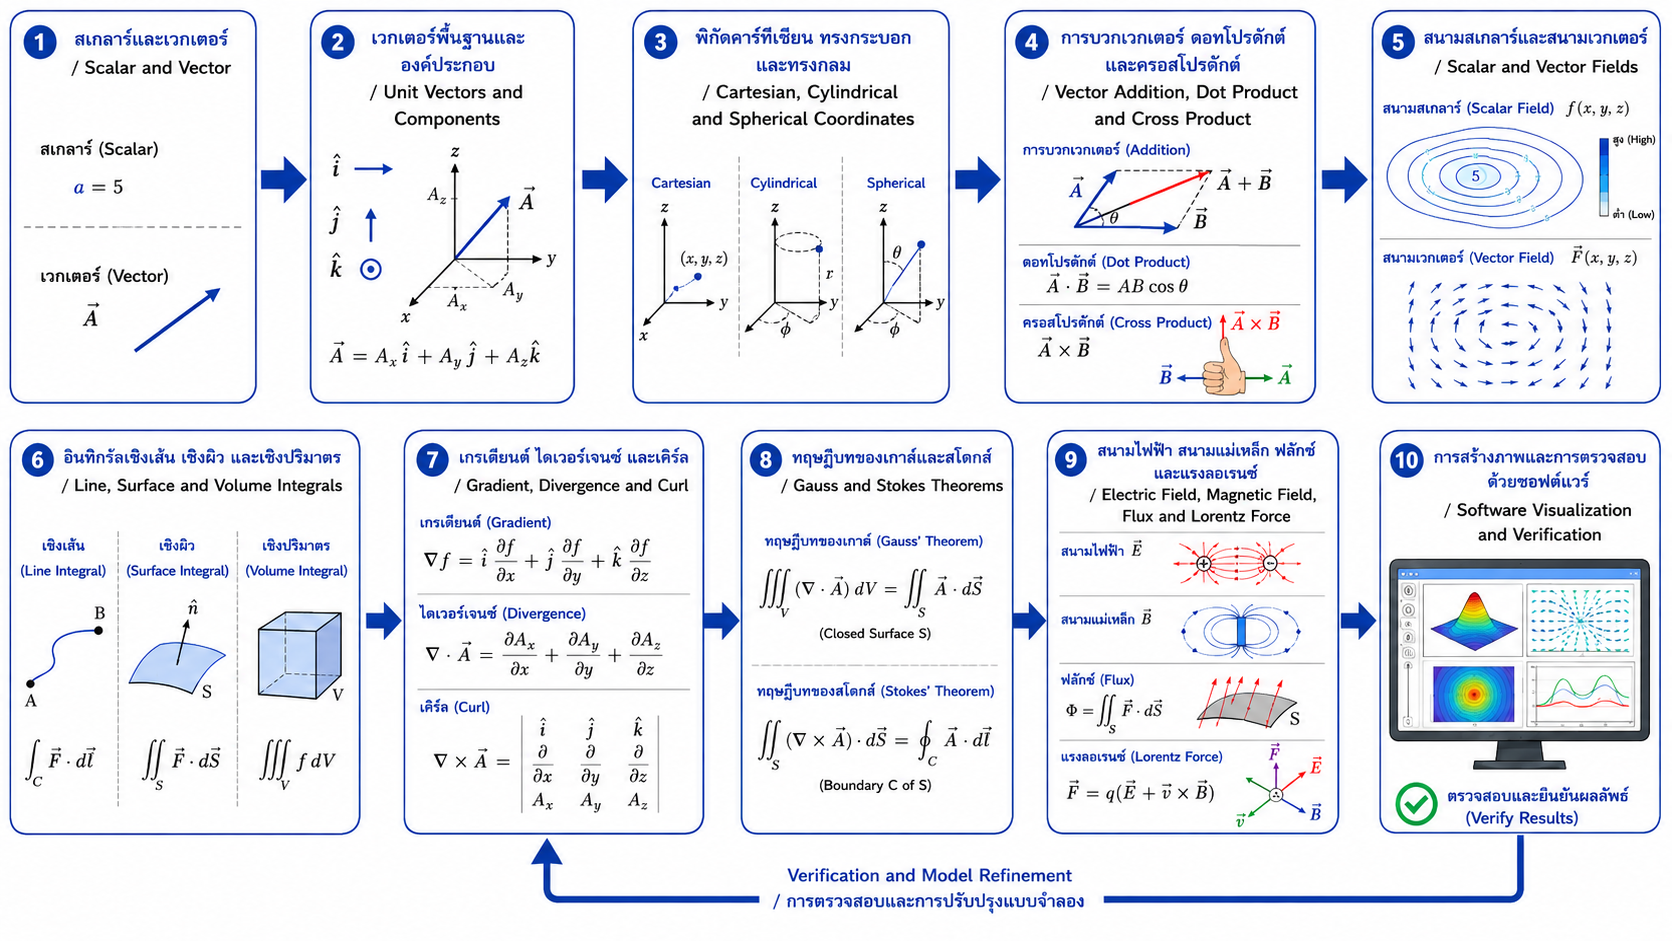
\includegraphics[width=0.8\textwidth]{images/chapter3/figure-01.png}
    \caption{แผนผังการเรียนรู้การวิเคราะห์เวกเตอร์สู่การประยุกต์สนามแม่เหล็กไฟฟ้า}
\end{figure}

\newpage

\subsection{6. บทนำ}

ในวงจรไฟฟ้าแบบรวมศูนย์ เรามักใช้แรงดันและกระแสเป็นค่าที่ขึ้นกับเวลา แต่เมื่อพิจารณาระบบที่มีมิติทางกายภาพ เช่น สายส่ง เสาอากาศ มอเตอร์ไฟฟ้า หม้อแปลง ตัวเก็บประจุ แผ่นนำไฟฟ้า หรือบริเวณรอบตัวนำ ปริมาณทางไฟฟ้าและแม่เหล็กจะแตกต่างกันตามตำแหน่งและทิศทาง การระบุเพียงค่าเดียวจึงไม่เพียงพอ

ตัวอย่างเช่น สนามไฟฟ้ารอบประจุบวกชี้ออกจากประจุในทุกทิศทาง ขณะที่สนามแม่เหล็กรอบลวดตัวนำตรงที่มีกระแสไหลมีทิศเป็นวงกลมล้อมรอบตัวนำ ทิศของแรงบนประจุที่เคลื่อนที่ในสนามแม่เหล็กตั้งฉากกับทั้งทิศความเร็วและทิศสนาม ปรากฏการณ์เหล่านี้ต้องใช้เวกเตอร์และสนามเวกเตอร์ในการอธิบาย

การวิเคราะห์เวกเตอร์ยังช่วยให้กฎทางฟิสิกส์มีรูปแบบกระชับและมีความหมายชัดเจน เช่น

\begin{itemize}
\item \(\mathbf{E}=-\nabla V\) แสดงว่าสนามไฟฟ้าชี้ไปทางที่ศักย์ไฟฟ้าลดลงเร็วที่สุด
\item \(\nabla\cdot\mathbf{D}=\rho_v\) แสดงความสัมพันธ์เฉพาะที่ระหว่างความหนาแน่นฟลักซ์ไฟฟ้ากับความหนาแน่นประจุปริมาตร
\item \(\nabla\cdot\mathbf{B}=0\) สะท้อนว่าเส้นแรงแม่เหล็กไม่มีจุดเริ่มหรือจุดสิ้นสุดแบบประจุแม่เหล็กเดี่ยวในทฤษฎีมาตรฐาน
\item \(\mathbf{F}=q(\mathbf{E}+\mathbf{v}\times\mathbf{B})\) เชื่อมสนามไฟฟ้า สนามแม่เหล็ก และแรงที่กระทำต่อประจุ
\end{itemize}

จุดมุ่งหมายของบทนี้จึงไม่ใช่ให้ผู้เรียนจำสมการจำนวนมาก แต่ให้สามารถมองเห็นโครงสร้างของสนาม เลือกระบบพิกัดให้สอดคล้องกับสมมาตร เลือกผลคูณเวกเตอร์ให้เหมาะกับความหมาย และแปลผลคำนวณกลับไปสู่ปรากฏการณ์ทางวิศวกรรม

\subsection{7. เนื้อหาหลัก การวิเคราะห์เวกเตอร์สำหรับงานวิศวกรรมไฟฟ้า}

\subsubsection{7.1 ความหมายของสเกลาร์และเวกเตอร์}

\paragraph{7.1.1 ปริมาณสเกลาร์}

\textbf{สเกลาร์ (Scalar)} เป็นปริมาณที่กำหนดได้ด้วยขนาดและหน่วย โดยไม่ต้องระบุทิศทาง ตัวอย่างในงานวิศวกรรมไฟฟ้า ได้แก่ ประจุไฟฟ้า ศักย์ไฟฟ้า พลังงาน กำลังไฟฟ้า ความต้านทาน และอุณหภูมิ สเกลาร์อาจเป็นบวก ลบ หรือศูนย์ เครื่องหมายลบไม่ได้หมายถึงทิศทางในอวกาศเสมอไป แต่อาจหมายถึงค่าที่ต่ำกว่าจุดอ้างอิงหรือทิศการถ่ายโอนที่กำหนดตามอนุสัญญา

\paragraph{7.1.2 ปริมาณเวกเตอร์}

\textbf{เวกเตอร์ (Vector)} เป็นปริมาณที่ต้องระบุทั้งขนาดและทิศทาง ตัวอย่าง ได้แก่ ตำแหน่ง \(\mathbf{r}\) ความเร็ว \(\mathbf{v}\) แรง \(\mathbf{F}\) สนามไฟฟ้า \(\mathbf{E}\) ความหนาแน่นฟลักซ์ไฟฟ้า \(\mathbf{D}\) ความเข้มสนามแม่เหล็ก \(\mathbf{H}\) ความหนาแน่นฟลักซ์แม่เหล็ก \(\mathbf{B}\) และความหนาแน่นกระแส \(\mathbf{J}\)

\paragraph{7.1.3 การแทนเวกเตอร์ในพิกัดฉาก}

\[
\mathbf{A}=A_x\mathbf{a}_x+A_y\mathbf{a}_y+A_z\mathbf{a}_z
\]

โดย \(A_x,A_y,A_z\) คือองค์ประกอบตามแกน และ \(\mathbf{a}_x,\mathbf{a}_y,\mathbf{a}_z\) คือเวกเตอร์หนึ่งหน่วย ขนาดของเวกเตอร์คือ

\[
|\mathbf{A}|=\sqrt{A_x^2+A_y^2+A_z^2}
\]

สูตรนี้ใช้เมื่อแกนทั้งสามตั้งฉากกันและเวกเตอร์หนึ่งหน่วยมีขนาดหนึ่ง

% [รูปที่ 2: การแยกเวกเตอร์สามมิติเป็นองค์ประกอบตามแกน]
% ประเภทภาพ: Technical Illustration
% ตำแหน่งที่แนะนำ: หลังหัวข้อ 7.1.3
% วัตถุประสงค์การเรียนรู้: เชื่อมเวกเตอร์เชิงเรขาคณิตกับองค์ประกอบพีชคณิต
% คำอธิบายภาพ: แสดงเวกเตอร์ $\mathbf{A}$ จากจุดกำเนิดไปยังจุด $(A_x,A_y,A_z)$ พร้อมเส้นฉายตั้งฉากและลูกศรองค์ประกอบ
% องค์ประกอบที่ต้องมี: แกน $x,y,z$ จุดกำเนิด เวกเตอร์หลัก เส้นฉายประ และป้ายองค์ประกอบ
% ภาษาของป้ายกำกับ: ไทยและอังกฤษ
% สัดส่วนภาพ: 16:9
% Image Generation Prompt: Clean 3D engineering textbook illustration of a vector A from the origin to point (Ax, Ay, Az) in a Cartesian coordinate system. Show orthogonal projections and component arrows Ax ax, Ay ay and Az az, dashed projection lines, labeled x-y-z axes, white background, precise blue technical line art, 16:9.
% Alt Text: เวกเตอร์สามมิติถูกแยกเป็นองค์ประกอบตามแกนตั้งฉาก $x,y,z$

\begin{figure}[htbp]
    \centering
    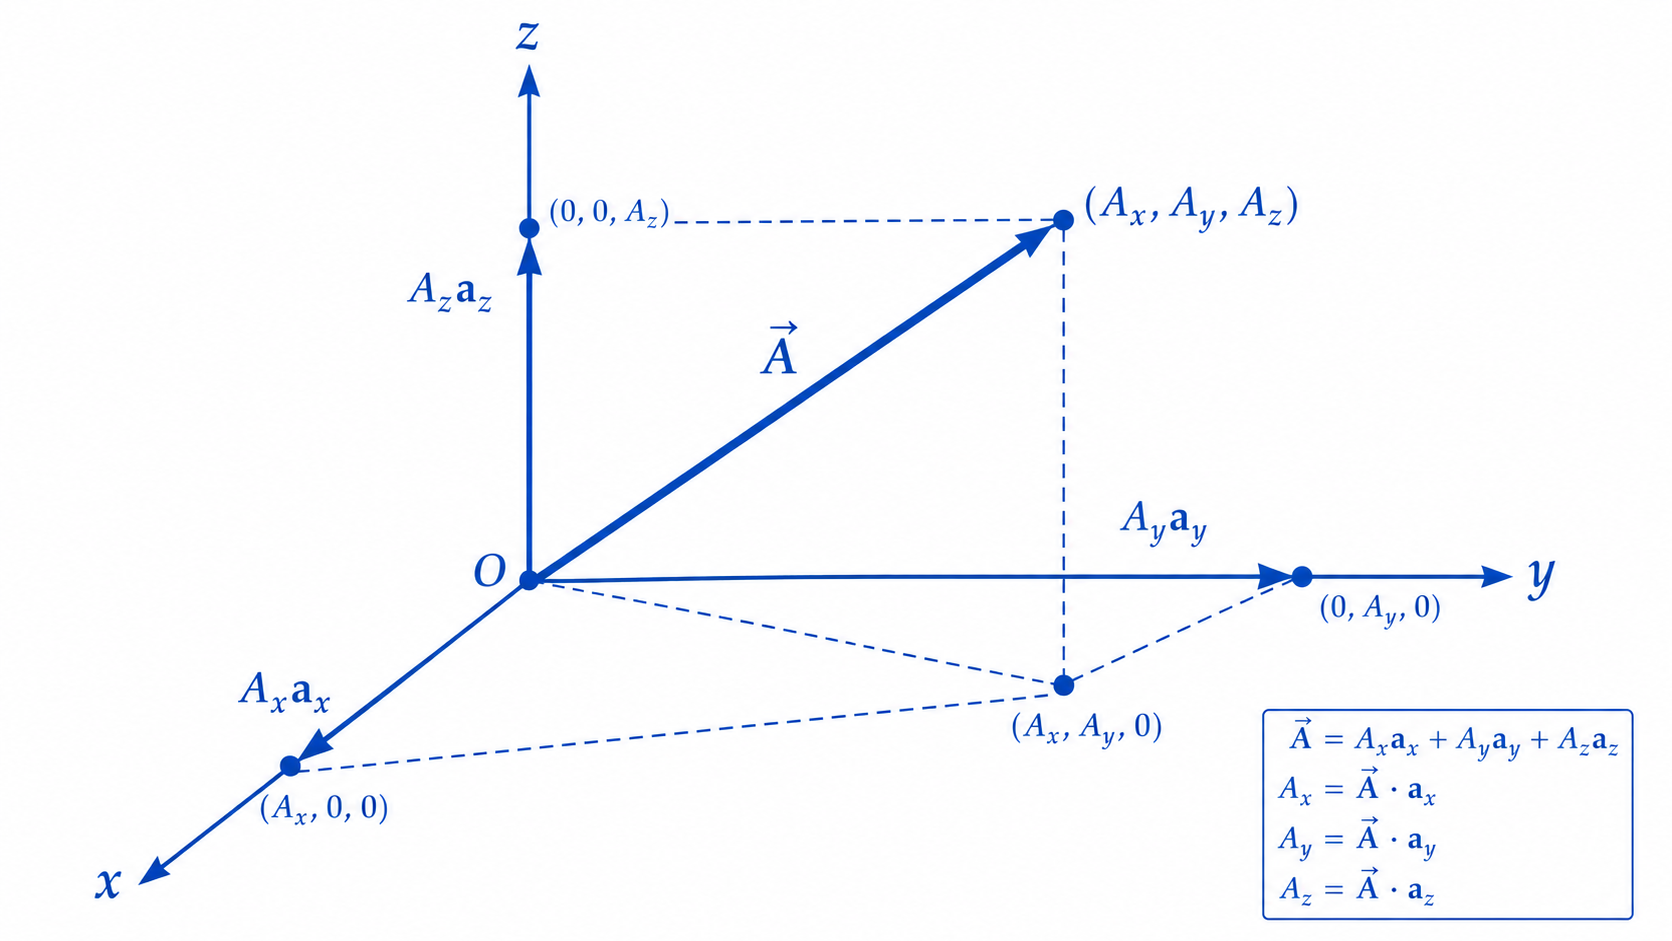
\includegraphics[width=0.8\textwidth]{images/chapter3/figure-02.png}
    \caption{การแยกเวกเตอร์สามมิติเป็นองค์ประกอบตามแกน}
\end{figure}

\paragraph{ตัวอย่างที่ 1 การหาขนาดและเวกเตอร์หนึ่งหน่วย}

กำหนดให้

\[
\mathbf{A}=3\mathbf{a}_x-2\mathbf{a}_y+6\mathbf{a}_z
\]

ขนาดคือ

\[
|\mathbf{A}|=\sqrt{3^2+(-2)^2+6^2}=7
\]

เวกเตอร์หนึ่งหน่วยคือ

\[
\boxed{\mathbf{a}_A=\frac{3}{7}\mathbf{a}_x-\frac{2}{7}\mathbf{a}_y+\frac{6}{7}\mathbf{a}_z}
\]

ตรวจสอบได้ว่า \(|\mathbf{a}_A|=1\) เครื่องหมายลบขององค์ประกอบ \(y\) แสดงว่ามีส่วนชี้ตรงข้ามแกน \(y\) บวก


\subsubsection{7.2 ระบบพิกัดที่ใช้ในงานวิศวกรรมไฟฟ้า}

การเลือกระบบพิกัดที่สอดคล้องกับสมมาตรช่วยลดจำนวนตัวแปรและทำให้สมการง่ายขึ้น

\paragraph{7.2.1 ระบบพิกัดฉาก}

จุดเขียนเป็น \(P(x,y,z)\) และ

\[
\mathbf{r}=x\mathbf{a}_x+y\mathbf{a}_y+z\mathbf{a}_z
\]

\[
d\mathbf{l}=dx\mathbf{a}_x+dy\mathbf{a}_y+dz\mathbf{a}_z,\qquad
dV=dx\,dy\,dz
\]

เหมาะกับแผ่นระนาบ กล่อง และระบบที่เปลี่ยนตามแกนตรง

\paragraph{7.2.2 ระบบพิกัดทรงกระบอก}

จุดเขียนเป็น \(P(\rho,\phi,z)\) โดย

\[
x=\rho\cos\phi,\qquad y=\rho\sin\phi
\]

\[
\rho=\sqrt{x^2+y^2},\qquad \phi=\operatorname{atan2}(y,x)
\]

เวกเตอร์หนึ่งหน่วยสัมพันธ์กับพิกัดฉากดังนี้

\[
\mathbf{a}_\rho=\cos\phi\,\mathbf{a}_x+\sin\phi\,\mathbf{a}_y
\]

\[
\mathbf{a}_\phi=-\sin\phi\,\mathbf{a}_x+\cos\phi\,\mathbf{a}_y
\]

\[
d\mathbf{l}=d\rho\,\mathbf{a}_\rho+\rho d\phi\,\mathbf{a}_\phi+dz\,\mathbf{a}_z
\]

\[
dV=\rho\,d\rho\,d\phi\,dz
\]

เหมาะกับลวดตรง สายโคแอกเชียล และระบบสมมาตรรอบแกน

\paragraph{7.2.3 ระบบพิกัดทรงกลม}

ใช้อนุสัญญา \(P(r,\theta,\phi)\) โดย \(\theta\) วัดลงจากแกน \(z\) บวก และ \(\phi\) วัดในระนาบ \(xy\)

\[
x=r\sin\theta\cos\phi,\quad
y=r\sin\theta\sin\phi,\quad
z=r\cos\theta
\]

\[
d\mathbf{l}=dr\,\mathbf{a}_r+r\,d\theta\,\mathbf{a}_\theta+r\sin\theta\,d\phi\,\mathbf{a}_\phi
\]

\[
dV=r^2\sin\theta\,dr\,d\theta\,d\phi
\]

เหมาะกับประจุจุด ตัวนำทรงกลม และระบบสมมาตรรอบจุด

\begin{quote}
\textbf{ข้อควรระวัง:} ตำราบางเล่มสลับสัญลักษณ์ \(\theta\) กับ \(\phi\) จึงต้องตรวจอนุสัญญาก่อนใช้สูตร
\end{quote}

\paragraph{7.2.4 การเลือกระบบพิกัดจากสมมาตร}

\begin{table}[htbp]
    \centering
    \begin{tabularx}{\textwidth}{L{0.25\textwidth} L{0.27\textwidth} Y}
        \hline
        \textbf{ลักษณะระบบ} & \textbf{ระบบพิกัดที่มักเหมาะสม} & \textbf{ตัวอย่าง} \\
        \hline
        สมมาตรตามระนาบ & พิกัดฉาก & ตัวเก็บประจุแผ่นขนาน \\
        สมมาตรรอบแกน & ทรงกระบอก & ลวดตรง สายโคแอกเชียล \\
        สมมาตรรอบจุด & ทรงกลม & สนามจากประจุจุด \\
        ไม่มีสมมาตรเด่น & พิกัดฉาก/เชิงตัวเลข & อิเล็กโทรดรูปทรงซับซ้อน \\
        \hline
    \end{tabularx}
\end{table}

% [รูปที่ 3: เปรียบเทียบระบบพิกัดฉาก ทรงกระบอก และทรงกลม]
% ประเภทภาพ: Technical Illustration / Infographic
% ตำแหน่งที่แนะนำ: หลังหัวข้อ 7.2.4
% วัตถุประสงค์การเรียนรู้: เห็นนิยามพิกัดและสมมาตรที่เหมาะกับแต่ละระบบ
% คำอธิบายภาพ: สามส่วนแสดงจุดเดียวกันในพิกัดฉาก ทรงกระบอก และทรงกลม พร้อมมุม ระยะ และเวกเตอร์หนึ่งหน่วย
% องค์ประกอบที่ต้องมี: แกนพิกัด เส้นรัศมี ส่วนโค้งมุม และตัวอย่างแผ่นขนาน ลวดตรง ประจุจุด
% ภาษาของป้ายกำกับ: ไทยและอังกฤษ
% สัดส่วนภาพ: 16:9
% Image Generation Prompt: Three-panel engineering textbook comparison of Cartesian, cylindrical and spherical coordinate systems, showing the same point in space with coordinates (x,y,z), (rho,phi,z), and (r,theta,phi). Include axes, projection lines, angle arcs, radial distances, local unit vectors, and small application icons for parallel plates, a long wire, and a point charge. White background, accurate blue technical line art, Thai-English labels, 16:9.
% Alt Text: เปรียบเทียบพิกัดสามระบบและตัวอย่างสมมาตรที่เหมาะสม

\begin{figure}[htbp]
    \centering
    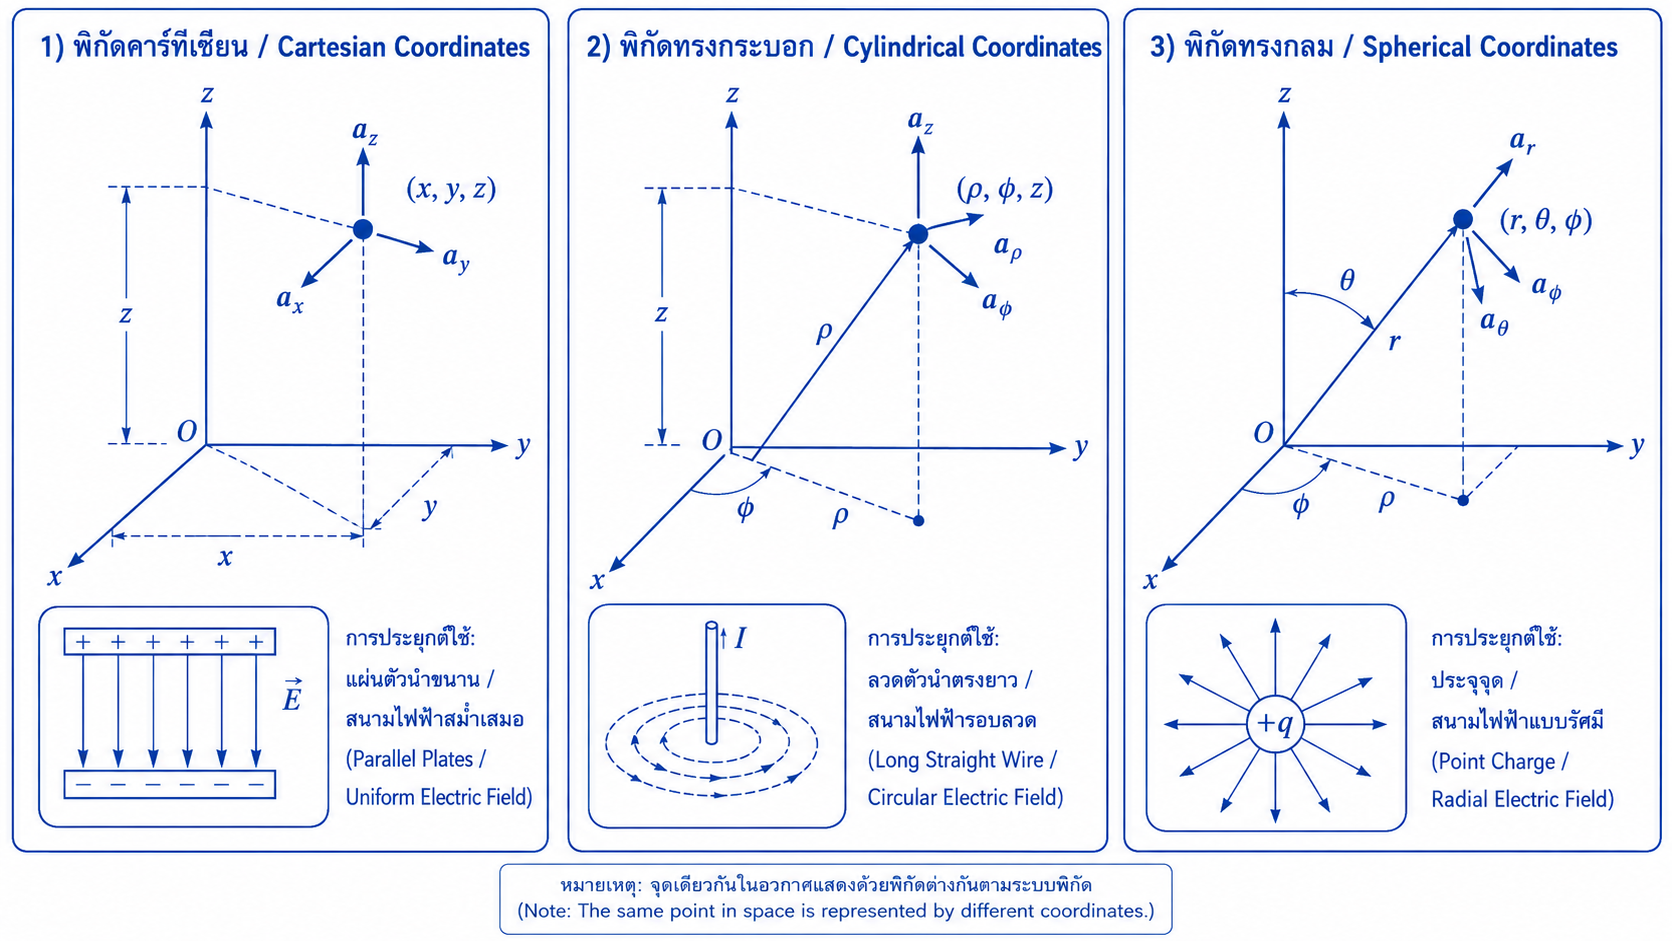
\includegraphics[width=0.8\textwidth]{images/chapter3/figure-03.png}
    \caption{เปรียบเทียบระบบพิกัดฉาก ทรงกระบอก และทรงกลม}
\end{figure}

\paragraph{ตัวอย่างที่ 2 การแปลงพิกัด}

ให้ \(P=(3,4,5)\)

พิกัดทรงกระบอก:

\[
\rho=5,\qquad \phi=\tan^{-1}(4/3)=53.13^\circ
\]

\[
\boxed{P=(5,53.13^\circ,5)}
\]

พิกัดทรงกลม:

\[
r=\sqrt{50}=7.071,\qquad
\theta=\cos^{-1}(5/7.071)=45.00^\circ
\]

\[
\boxed{P=(7.071,45.00^\circ,53.13^\circ)}
\]

\subsubsection{7.3 การบวก ลบ และการคูณเวกเตอร์}

เมื่อเวกเตอร์อยู่ในฐานเดียวกัน

\[
\mathbf{A}\pm\mathbf{B}
=(A_x\pm B_x)\mathbf{a}_x
+(A_y\pm B_y)\mathbf{a}_y
+(A_z\pm B_z)\mathbf{a}_z
\]

การคูณด้วยสเกลาร์ \(k\) ให้ \(k\mathbf{A}\) หาก \(k<0\) ทิศเวกเตอร์กลับตรงข้าม

สำหรับจุด \(P_1(x_1,y_1,z_1)\) และ \(P_2(x_2,y_2,z_2)\)

\[
\mathbf{R}_{12}=(x_2-x_1)\mathbf{a}_x+(y_2-y_1)\mathbf{a}_y+(z_2-z_1)\mathbf{a}_z
\]

\[
R_{12}=|\mathbf{R}_{12}|,\qquad
\mathbf{a}_{12}=\frac{\mathbf{R}_{12}}{R_{12}}
\]

ความสัมพันธ์นี้สำคัญต่อการหาทิศสนามจากแหล่งกำเนิดไปยังจุดสังเกต

\subsubsection{7.4 ดอตโปรดักต์และการประยุกต์กับงานและพลังงาน}

\paragraph{7.4.1 นิยามและความหมาย}

ดอตโปรดักต์หรือผลคูณเชิงสเกลาร์นิยามเป็น

\[
\mathbf{A}\cdot\mathbf{B}=|\mathbf{A}||\mathbf{B}|\cos\theta
\]

โดย \(\theta\) คือมุมระหว่างเวกเตอร์ ผลลัพธ์เป็นสเกลาร์

\begin{itemize}
\item \(\theta=0^\circ\): ผลคูณเป็นบวกสูงสุด
\item \(\theta=90^\circ\): ผลคูณเป็นศูนย์
\item \(90^\circ<\theta\leq180^\circ\): ผลคูณเป็นลบ
\end{itemize}

ในพิกัดฉาก

\[
\mathbf{A}\cdot\mathbf{B}=A_xB_x+A_yB_y+A_zB_z
\]

องค์ประกอบเชิงสเกลาร์ของ \(\mathbf{A}\) ตามทิศเวกเตอร์หนึ่งหน่วย \(\mathbf{a}_u\) คือ

\[
A_u=\mathbf{A}\cdot\mathbf{a}_u
\]

เวกเตอร์ฉายคือ

\[
\operatorname{proj}_{\mathbf{a}_u}\mathbf{A}
=(\mathbf{A}\cdot\mathbf{a}_u)\mathbf{a}_u
\]

\paragraph{7.4.2 งานจากแรงและสนามไฟฟ้า}

งานย่อยจากแรง \(\mathbf{F}\) เมื่อเคลื่อนที่ \(d\mathbf{l}\) คือ

\[
dW=\mathbf{F}\cdot d\mathbf{l}
\]

งานรวมตามเส้นทาง \(C\) คือ

\[
W=\int_C\mathbf{F}\cdot d\mathbf{l}
\]

สำหรับประจุ \(q\) ในสนามไฟฟ้า \(\mathbf{E}\)

\[
W=q\int_C\mathbf{E}\cdot d\mathbf{l}
\]

หน่วยคือ \(\text{N}\cdot\text{m}=\text{J}\) ดอตโปรดักต์เลือกเฉพาะองค์ประกอบของแรงตามทิศการเคลื่อนที่

% [รูปที่ 4: ความหมายเชิงเรขาคณิตของดอตโปรดักต์และครอสโปรดักต์]
% ประเภทภาพ: Infographic / Technical Illustration
% ตำแหน่งที่แนะนำ: หลังหัวข้อ 7.4.2
% วัตถุประสงค์การเรียนรู้: เปรียบเทียบผลคูณที่ให้การฉายกับผลคูณที่ให้เวกเตอร์ตั้งฉาก
% คำอธิบายภาพ: ด้านซ้ายแสดงมุมและเงาฉายของเวกเตอร์ ด้านขวาแสดงพื้นที่สี่เหลี่ยมด้านขนานและเวกเตอร์ปกติตามกฎมือขวา
% องค์ประกอบที่ต้องมี: มุม $\theta$ เส้นฉาย ลูกศรปกติ สูตรดอตและครอส
% ภาษาของป้ายกำกับ: ไทยและอังกฤษ
% สัดส่วนภาพ: 16:9
% Image Generation Prompt: Split-panel engineering textbook illustration comparing dot product and cross product. Left: vectors A and B with angle theta, projection of A onto B, formula A dot B = |A||B|cos theta, scalar result. Right: vectors A and B forming a parallelogram, normal vector A cross B determined by the right-hand rule, formula magnitude = |A||B|sin theta, vector result. White background, clean blue line art, Thai-English labels, 16:9.
% Alt Text: ดอตโปรดักต์แสดงองค์ประกอบตามแนว ส่วนครอสโปรดักต์แสดงเวกเตอร์ตั้งฉาก

\begin{figure}[htbp]
    \centering
    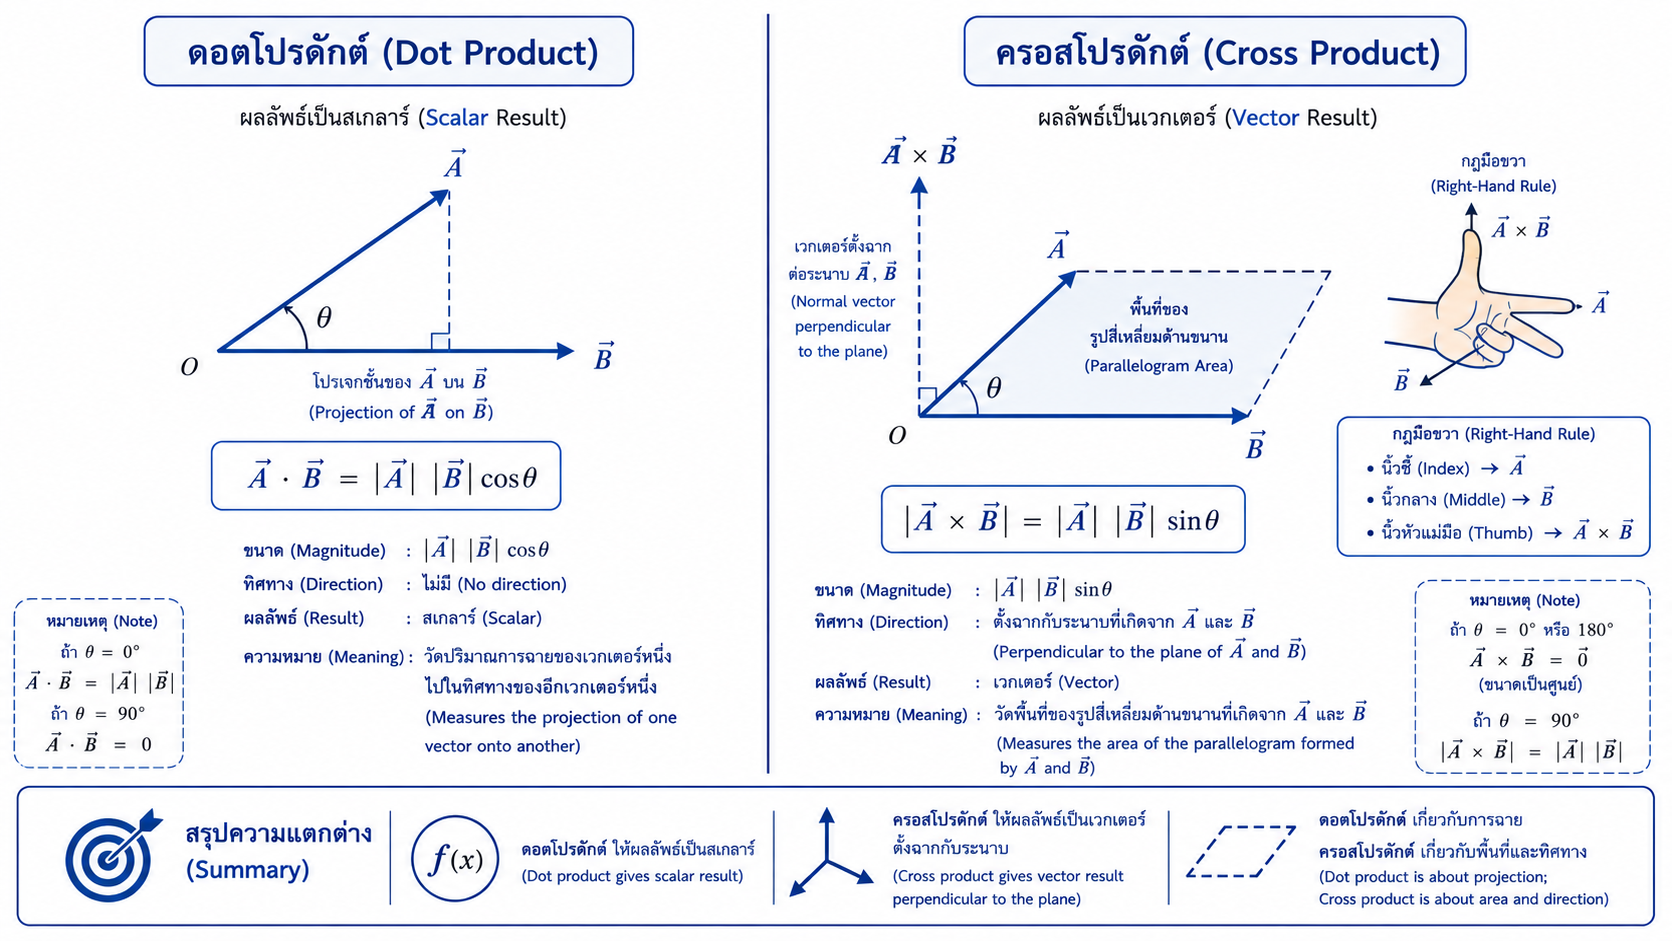
\includegraphics[width=0.8\textwidth]{images/chapter3/figure-04.png}
    \caption{ความหมายเชิงเรขาคณิตของดอตโปรดักต์และครอสโปรดักต์}
\end{figure}

\paragraph{ตัวอย่างที่ 3 ดอตโปรดักต์ มุม และการฉาย}

กำหนด

\[
\mathbf{A}=2\mathbf{a}_x-\mathbf{a}_y+3\mathbf{a}_z,\qquad
\mathbf{B}=\mathbf{a}_x+4\mathbf{a}_y-2\mathbf{a}_z
\]

\begin{enumerate}
\item ดอตโปรดักต์
\end{enumerate}

\[
\mathbf{A}\cdot\mathbf{B}=2-4-6=-8
\]

\begin{enumerate}
\setcounter{enumi}{1}
\item ขนาด
\end{enumerate}

\[
|\mathbf{A}|=\sqrt{14},\qquad |\mathbf{B}|=\sqrt{21}
\]

\begin{enumerate}
\setcounter{enumi}{2}
\item มุม
\end{enumerate}

\[
\cos\theta=\frac{-8}{\sqrt{294}}
\]

\[
\boxed{\theta\approx117.8^\circ}
\]

\begin{enumerate}
\setcounter{enumi}{3}
\item องค์ประกอบของ \(\mathbf{A}\) ตามทิศ \(\mathbf{B}\)
\end{enumerate}

\[
A_B=\frac{\mathbf{A}\cdot\mathbf{B}}{|\mathbf{B}|}
=\frac{-8}{\sqrt{21}}\approx-1.746
\]

ค่าลบแสดงว่าองค์ประกอบที่ฉายชี้สวนทางกับ \(\mathbf{B}\)

\subsubsection{7.5 ครอสโปรดักต์และการประยุกต์กับสนามแม่เหล็ก}

\paragraph{7.5.1 นิยาม}

\[
\mathbf{A}\times\mathbf{B}
=|\mathbf{A}||\mathbf{B}|\sin\theta\,\mathbf{a}_n
\]

\(\mathbf{a}_n\) ตั้งฉากกับระนาบของ \(\mathbf{A}\) และ \(\mathbf{B}\) ตามกฎมือขวา ขนาดของผลคูณเท่ากับพื้นที่สี่เหลี่ยมด้านขนาน

ในพิกัดฉาก

\[
\mathbf{A}\times\mathbf{B}
=
\begin{vmatrix}
\mathbf{a}_x & \mathbf{a}_y & \mathbf{a}_z\\
A_x & A_y & A_z\\
B_x & B_y & B_z
\end{vmatrix}
\]

\[
\mathbf{A}\times\mathbf{B}=-(\mathbf{B}\times\mathbf{A})
\]

\paragraph{7.5.2 แรงแม่เหล็กบนประจุเคลื่อนที่}

\[
\mathbf{F}_m=q\mathbf{v}\times\mathbf{B}
\]

\[
F_m=|q|vB\sin\theta
\]

หาก \(q<0\) ทิศแรงตรงข้ามกับทิศที่กฎมือขวาให้สำหรับประจุบวก

\paragraph{7.5.3 แรงบนตัวนำที่มีกระแส}

สำหรับตัวนำตรงในสนามแม่เหล็กสม่ำเสมอ

\[
\mathbf{F}=I\mathbf{L}\times\mathbf{B}
\]

สมการนี้เป็นพื้นฐานของมอเตอร์ ลำโพง และแอคชูเอเตอร์แม่เหล็กไฟฟ้า

\paragraph{ตัวอย่างที่ 4 แรงบนตัวนำในสนามแม่เหล็ก}

ตัวนำยาว \(0.30\) m วางตาม \(+x\) มีกระแส \(5\) A และอยู่ในสนาม

\[
\mathbf{B}=0.20\mathbf{a}_z\ \text{T}
\]

\[
\mathbf{L}=0.30\mathbf{a}_x\ \text{m}
\]

\[
\mathbf{F}=5(0.30\mathbf{a}_x)\times(0.20\mathbf{a}_z)
\]

เนื่องจาก \(\mathbf{a}_x\times\mathbf{a}_z=-\mathbf{a}_y\)

\[
\boxed{\mathbf{F}=-0.30\mathbf{a}_y\ \text{N}}
\]

ตรวจหน่วยได้ว่า \(\text{A}\cdot\text{m}\cdot\text{T}=\text{N}\)

\subsubsection{7.6 เวกเตอร์หนึ่งหน่วยและองค์ประกอบของเวกเตอร์}

สำหรับเวกเตอร์ไม่เป็นศูนย์

\[
\mathbf{a}_A=\frac{\mathbf{A}}{|\mathbf{A}|}
\]

ถ้า \(\alpha,\beta,\gamma\) เป็นมุมกับแกน \(x,y,z\)

\[
\cos\alpha=\frac{A_x}{|\mathbf{A}|},\quad
\cos\beta=\frac{A_y}{|\mathbf{A}|},\quad
\cos\gamma=\frac{A_z}{|\mathbf{A}|}
\]

\[
\cos^2\alpha+\cos^2\beta+\cos^2\gamma=1
\]

ในพิกัดฉาก เวกเตอร์หนึ่งหน่วยคงทิศทุกตำแหน่ง แต่ในพิกัดทรงกระบอกและทรงกลม ฐานบางตัวเปลี่ยนทิศตามตำแหน่ง เช่น \(\mathbf{a}_\rho\) และ \(\mathbf{a}_\phi\)

การแปลงองค์ประกอบจากฉากเป็นทรงกระบอก:

\[
A_\rho=A_x\cos\phi+A_y\sin\phi
\]

\[
A_\phi=-A_x\sin\phi+A_y\cos\phi,\qquad A_z=A_z
\]

ต้องประเมินที่มุม \(\phi\) ของตำแหน่งนั้น

\subsubsection{7.7 สนามเวกเตอร์ในงานไฟฟ้าและแม่เหล็ก}

\paragraph{7.7.1 สนามสเกลาร์และสนามเวกเตอร์}

สนามสเกลาร์ให้ค่าสเกลาร์ที่ทุกตำแหน่ง เช่น ศักย์ไฟฟ้า

\[
V=V(x,y,z)
\]

พื้นผิวที่ \(V\) คงที่เรียกว่า \textbf{พื้นผิวศักย์เท่ากัน}

สนามเวกเตอร์ให้เวกเตอร์ที่ทุกตำแหน่ง เช่น

\[
\mathbf{E}(x,y,z)=E_x\mathbf{a}_x+E_y\mathbf{a}_y+E_z\mathbf{a}_z
\]

หากขึ้นกับเวลาจะเขียน \(\mathbf{E}(\mathbf{r},t)\)

\paragraph{7.7.2 เส้นสนาม}

เส้นสนามเป็นเส้นสมมติที่เส้นสัมผัสมีทิศเดียวกับสนาม ณ จุดนั้น รูปแบบสำคัญได้แก่

\begin{itemize}
\item สนามสม่ำเสมอ: ลูกศรขนาดและทิศคงที่
\item สนามรัศมี: ชี้ออกหรือเข้าหาศูนย์กลาง
\item สนามวงกลม: ล้อมรอบแกน เช่น สนามแม่เหล็กรอบลวดตรง
\item สนามหมุนวนที่เกิดจากการเปลี่ยนตามเวลา
\end{itemize}

จำนวนเส้นในภาพไม่ใช่ค่าทางกายภาพโดยตรงหากไม่ได้กำหนดสเกล

% [รูปที่ 5: รูปแบบสนามเวกเตอร์ที่พบบ่อย]
% ประเภทภาพ: Infographic / Vector Field Illustration
% ตำแหน่งที่แนะนำ: หลังหัวข้อ 7.7.2
% วัตถุประสงค์การเรียนรู้: จำแนกสนามสม่ำเสมอ สนามรัศมี และสนามวงกลม
% คำอธิบายภาพ: สามช่อง ได้แก่ สนามสม่ำเสมอ สนามไฟฟ้ารัศมีออกจากประจุบวก และสนามแม่เหล็กวงกลมรอบลวดมีกระแส
% องค์ประกอบที่ต้องมี: ลูกศรสนาม ประจุบวก ลวดตรง กระแส $I$ และวงสนาม $\mathbf{B}$
% ภาษาของป้ายกำกับ: ไทยและอังกฤษ
% สัดส่วนภาพ: 16:9
% Image Generation Prompt: Three-panel educational vector field illustration: uniform field with parallel equal arrows; radial electric field pointing outward from a positive point charge with decreasing arrow length versus distance; circular magnetic field around a vertical current-carrying wire with current I upward and right-hand-rule direction. White background, blue engineering textbook style, Thai-English labels, 16:9.
% Alt Text: สนามสม่ำเสมอ สนามไฟฟ้ารัศมี และสนามแม่เหล็กวงกลมรอบลวด

\begin{figure}[htbp]
    \centering
    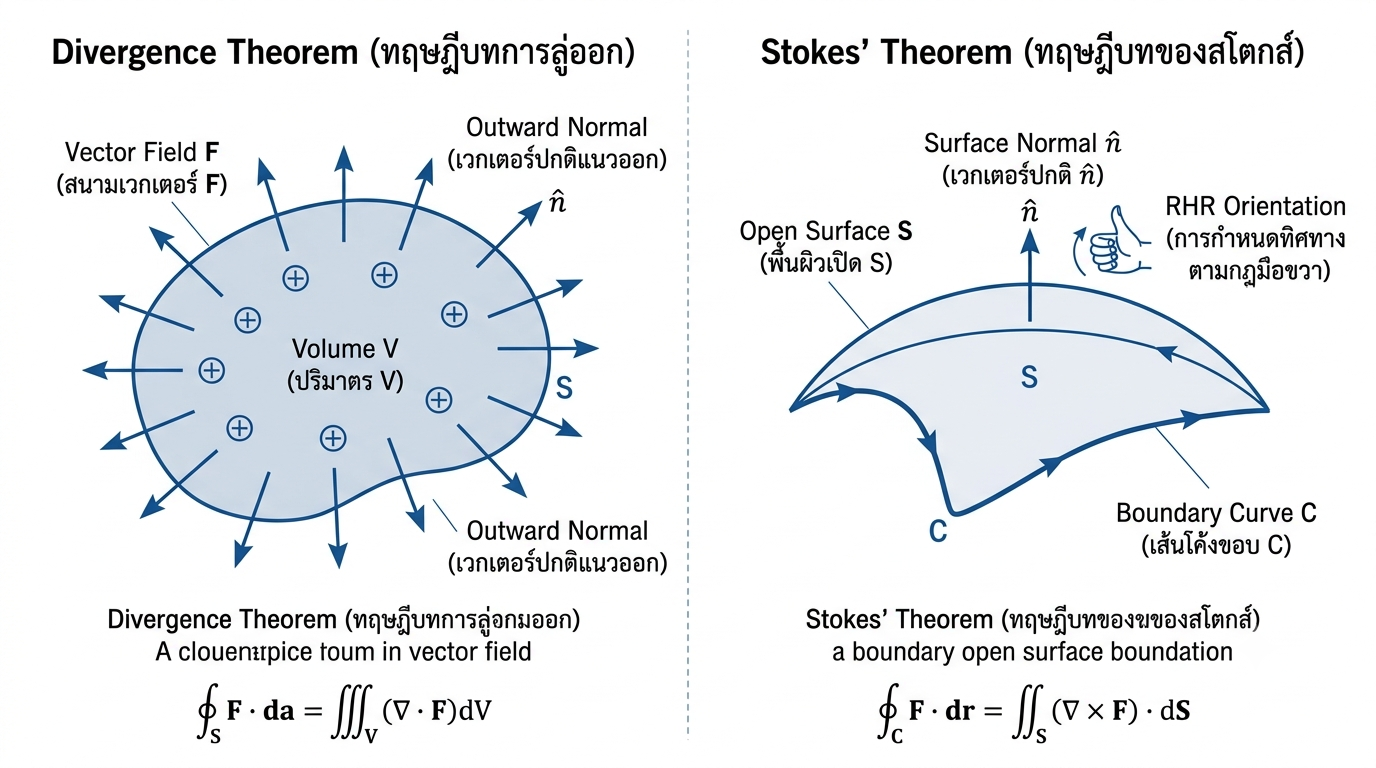
\includegraphics[width=0.8\textwidth]{images/chapter3/figure-05.png}
    \caption{รูปแบบสนามเวกเตอร์ที่พบบ่อย}
\end{figure}

\paragraph{7.7.3 สนามอนุรักษ์และความต่างศักย์}

สนามเรียกว่าอนุรักษ์เมื่ออินทิกรัลระหว่างสองจุดไม่ขึ้นกับเส้นทาง หรือ

\[
\oint_C\mathbf{E}\cdot d\mathbf{l}=0
\]

สำหรับสนามไฟฟ้าสถิต

\[
\mathbf{E}=-\nabla V
\]

\[
V_B-V_A=-\int_A^B\mathbf{E}\cdot d\mathbf{l}
\]

เครื่องหมายลบแสดงว่าสนามไฟฟ้าชี้ไปยังทิศที่ศักย์ลดลง

\subsubsection{7.8 อินทิกรัลเวกเตอร์สำหรับการวิเคราะห์สนาม}

\paragraph{7.8.1 อินทิกรัลเส้น}

\[
\int_C\mathbf{A}\cdot d\mathbf{l}
\]

ใช้คำนวณงาน ความต่างศักย์ และการไหลเวียนตามเส้นทาง

\paragraph{7.8.2 อินทิกรัลพื้นผิวและฟลักซ์}

\[
\Phi=\int_S\mathbf{A}\cdot d\mathbf{S}
\]

โดย \(d\mathbf{S}=\mathbf{a}_n dS\) ดอตโปรดักต์เลือกองค์ประกอบของสนามที่ทะลุผิว

\paragraph{7.8.3 อินทิกรัลปริมาตร}

\[
Q=\int_V\rho_v\,dV
\]

ถ้า \(\rho_v\) มีหน่วย C/m\(^3\) ผลรวม \(Q\) มีหน่วย C

\paragraph{7.8.4 ทิศของขอบเขต}

\begin{itemize}
\item เวกเตอร์ปกติของผิวปิดนิยมชี้ออก
\item ทิศเส้นขอบสัมพันธ์กับเวกเตอร์ปกติด้วยกฎมือขวา
\item การกลับทิศทำให้เครื่องหมายอินทิกรัลเปลี่ยน
\end{itemize}

\paragraph{ตัวอย่างที่ 5 อินทิกรัลเส้นของสนามอนุรักษ์}

ให้

\[
\mathbf{E}=2x\mathbf{a}_x+3y\mathbf{a}_y\ \text{V/m}
\]

จาก \(A=(0,0)\) ไป \(B=(1,2)\) สนามเป็นเกรเดียนต์ของ

\[
\psi=x^2+\frac{3}{2}y^2
\]

ดังนั้น

\[
\int_A^B\mathbf{E}\cdot d\mathbf{l}
=\psi(B)-\psi(A)=1+6=7
\]

\[
\boxed{\int_A^B\mathbf{E}\cdot d\mathbf{l}=7\ \text{V}}
\]

หากใช้ \(V\) เป็นศักย์ไฟฟ้าตาม \(\mathbf{E}=-\nabla V\) จะมีเครื่องหมายตรงข้าม

\subsubsection{7.9 เกรเดียนต์ ไดเวอร์เจนซ์ และเคิร์ล}

\paragraph{7.9.1 ตัวดำเนินการเดล}

ในพิกัดฉาก

\[
\nabla=\mathbf{a}_x\frac{\partial}{\partial x}
+\mathbf{a}_y\frac{\partial}{\partial y}
+\mathbf{a}_z\frac{\partial}{\partial z}
\]

\(\nabla\) เป็นตัวดำเนินการอนุพันธ์ ไม่ใช่เวกเตอร์ทางกายภาพธรรมดา

\paragraph{7.9.2 เกรเดียนต์}

สำหรับสนามสเกลาร์ \(V\)

\[
\nabla V=
\frac{\partial V}{\partial x}\mathbf{a}_x+
\frac{\partial V}{\partial y}\mathbf{a}_y+
\frac{\partial V}{\partial z}\mathbf{a}_z
\]

เกรเดียนต์ชี้ไปยังทิศที่ \(V\) เพิ่มเร็วที่สุด มีขนาดเป็นอัตราการเพิ่มสูงสุดต่อระยะ และตั้งฉากกับพื้นผิว \(V=\text{ค่าคงที่}\)

ในพิกัดทรงกระบอก

\[
\nabla V=
\frac{\partial V}{\partial\rho}\mathbf{a}_\rho+
\frac{1}{\rho}\frac{\partial V}{\partial\phi}\mathbf{a}_\phi+
\frac{\partial V}{\partial z}\mathbf{a}_z
\]

ในพิกัดทรงกลม

\[
\nabla V=
\frac{\partial V}{\partial r}\mathbf{a}_r+
\frac{1}{r}\frac{\partial V}{\partial\theta}\mathbf{a}_\theta+
\frac{1}{r\sin\theta}\frac{\partial V}{\partial\phi}\mathbf{a}_\phi
\]

\paragraph{ตัวอย่างที่ 6 สนามไฟฟ้าจากศักย์}

ให้

\[
V=10-2x^2-y^2-3z\ \text{V}
\]

\[
\nabla V=-4x\mathbf{a}_x-2y\mathbf{a}_y-3\mathbf{a}_z
\]

\[
\mathbf{E}=-\nabla V
=4x\mathbf{a}_x+2y\mathbf{a}_y+3\mathbf{a}_z
\]

ที่ \((1,-2,0)\)

\[
\boxed{\mathbf{E}=4\mathbf{a}_x-4\mathbf{a}_y+3\mathbf{a}_z\ \text{V/m}}
\]

\[
|\mathbf{E}|=\sqrt{41}\approx6.403\ \text{V/m}
\]

\paragraph{7.9.3 ไดเวอร์เจนซ์}

\[
\nabla\cdot\mathbf{A}
=\frac{\partial A_x}{\partial x}
+\frac{\partial A_y}{\partial y}
+\frac{\partial A_z}{\partial z}
\]

ผลเป็นสเกลาร์และบอกฟลักซ์แผ่ออกสุทธิต่อหน่วยปริมาตร

\begin{itemize}
\item บวก: แหล่งกำเนิดสุทธิ
\item ลบ: แหล่งดูดสุทธิ
\item ศูนย์: ไม่มีการไหลออกสุทธิ ณ จุดนั้น แต่สนามอาจไม่เป็นศูนย์
\end{itemize}

ในพิกัดทรงกระบอก

\[
\nabla\cdot\mathbf{A}
=\frac{1}{\rho}\frac{\partial(\rho A_\rho)}{\partial\rho}
+\frac{1}{\rho}\frac{\partial A_\phi}{\partial\phi}
+\frac{\partial A_z}{\partial z}
\]

ในพิกัดทรงกลม

\[
\nabla\cdot\mathbf{A}
=\frac{1}{r^2}\frac{\partial(r^2A_r)}{\partial r}
+\frac{1}{r\sin\theta}\frac{\partial(\sin\theta A_\theta)}{\partial\theta}
+\frac{1}{r\sin\theta}\frac{\partial A_\phi}{\partial\phi}
\]

\paragraph{ตัวอย่างที่ 7 การหาไดเวอร์เจนซ์}

\[
\mathbf{A}=x^2\mathbf{a}_x+xy\mathbf{a}_y+z^2\mathbf{a}_z
\]

\[
\nabla\cdot\mathbf{A}=2x+x+2z=3x+2z
\]

ที่ \((1,2,3)\)

\[
\boxed{\nabla\cdot\mathbf{A}=9}
\]

\paragraph{7.9.4 เคิร์ล}

ในพิกัดฉาก

\[
\nabla\times\mathbf{A}
=
\begin{vmatrix}
\mathbf{a}_x & \mathbf{a}_y & \mathbf{a}_z\\
\dfrac{\partial}{\partial x} & \dfrac{\partial}{\partial y} & \dfrac{\partial}{\partial z}\\
A_x & A_y & A_z
\end{vmatrix}
\]

หรือ

\[
\nabla\times\mathbf{A}
=\left(\frac{\partial A_z}{\partial y}-\frac{\partial A_y}{\partial z}\right)\mathbf{a}_x
+\left(\frac{\partial A_x}{\partial z}-\frac{\partial A_z}{\partial x}\right)\mathbf{a}_y
+\left(\frac{\partial A_y}{\partial x}-\frac{\partial A_x}{\partial y}\right)\mathbf{a}_z
\]

ผลเป็นเวกเตอร์บอกแกนและความเข้มของแนวโน้มการหมุนวนเฉพาะที่

ในพิกัดทรงกระบอก

\[
\begin{aligned}
\nabla\times\mathbf{A}
={}&\frac{1}{\rho}\left[\frac{\partial A_z}{\partial\phi}
-\frac{\partial(\rho A_\phi)}{\partial z}\right]\mathbf{a}_\rho\\
&+\left[\frac{\partial A_\rho}{\partial z}
-\frac{\partial A_z}{\partial\rho}\right]\mathbf{a}_\phi\\
&+\frac{1}{\rho}\left[\frac{\partial(\rho A_\phi)}{\partial\rho}
-\frac{\partial A_\rho}{\partial\phi}\right]\mathbf{a}_z
\end{aligned}
\]

ในพิกัดทรงกลม

\[
\begin{aligned}
\nabla\times\mathbf{A}
={}&\frac{1}{r\sin\theta}
\left[\frac{\partial(\sin\theta A_\phi)}{\partial\theta}
-\frac{\partial A_\theta}{\partial\phi}\right]\mathbf{a}_r\\
&+\frac{1}{r}
\left[\frac{1}{\sin\theta}\frac{\partial A_r}{\partial\phi}
-\frac{\partial(rA_\phi)}{\partial r}\right]\mathbf{a}_\theta\\
&+\frac{1}{r}
\left[\frac{\partial(rA_\theta)}{\partial r}
-\frac{\partial A_r}{\partial\theta}\right]\mathbf{a}_\phi
\end{aligned}
\]

\paragraph{ตัวอย่างที่ 8 สนามหมุน}

\[
\mathbf{A}=-y\mathbf{a}_x+x\mathbf{a}_y
\]

\[
\nabla\times\mathbf{A}
=\left(\frac{\partial x}{\partial x}
-\frac{\partial(-y)}{\partial y}\right)\mathbf{a}_z
=2\mathbf{a}_z
\]

\[
\boxed{\nabla\times\mathbf{A}=2\mathbf{a}_z}
\]

สนามหมุนทวนเข็มนาฬิกาเมื่อมองจาก \(+z\)

\paragraph{7.9.5 เอกลักษณ์เวกเตอร์สำคัญ}

เมื่อฟังก์ชันเรียบเพียงพอ

\[
\nabla\times(\nabla V)=\mathbf{0}
\]

\[
\nabla\cdot(\nabla\times\mathbf{A})=0
\]

\[
\nabla^2V=\nabla\cdot(\nabla V)
\]

\(\nabla^2V\) เรียกว่า \textbf{ลาปลาเซียน} และเป็นพื้นฐานของสมการลาปลาซและปัวซอง

% [รูปที่ 6: ความหมายเชิงภาพของเกรเดียนต์ ไดเวอร์เจนซ์ และเคิร์ล]
% ประเภทภาพ: Infographic
% ตำแหน่งที่แนะนำ: หลังหัวข้อ 7.9.5
% วัตถุประสงค์การเรียนรู้: แยกความหมายของตัวดำเนินการทั้งสาม
% คำอธิบายภาพ: เกรเดียนต์บนเส้นชั้นค่า ไดเวอร์เจนซ์แบบแหล่งกำเนิด/แหล่งดูด และเคิร์ลพร้อมใบพัดเล็ก
% องค์ประกอบที่ต้องมี: เส้นชั้นค่า ลูกศร $\nabla V$ กล่องฟลักซ์เข้า–ออก และแกนหมุน
% ภาษาของป้ายกำกับ: ไทยและอังกฤษ
% สัดส่วนภาพ: 16:9
% Image Generation Prompt: Three-panel educational engineering infographic explaining gradient, divergence and curl. Gradient panel: scalar contour map with gradient arrow normal to contours toward maximum increase. Divergence panel: small control volumes showing source, sink and zero-net-flow cases. Curl panel: circulating vector field with a tiny paddle wheel and rotation axis following the right-hand rule. White background, blue technical textbook style, Thai-English labels, 16:9.
% Alt Text: เกรเดียนต์เป็นทิศเพิ่มสูงสุด ไดเวอร์เจนซ์เป็นการไหลออกสุทธิ และเคิร์ลเป็นการหมุนวนเฉพาะที่

\begin{figure}[htbp]
    \centering
    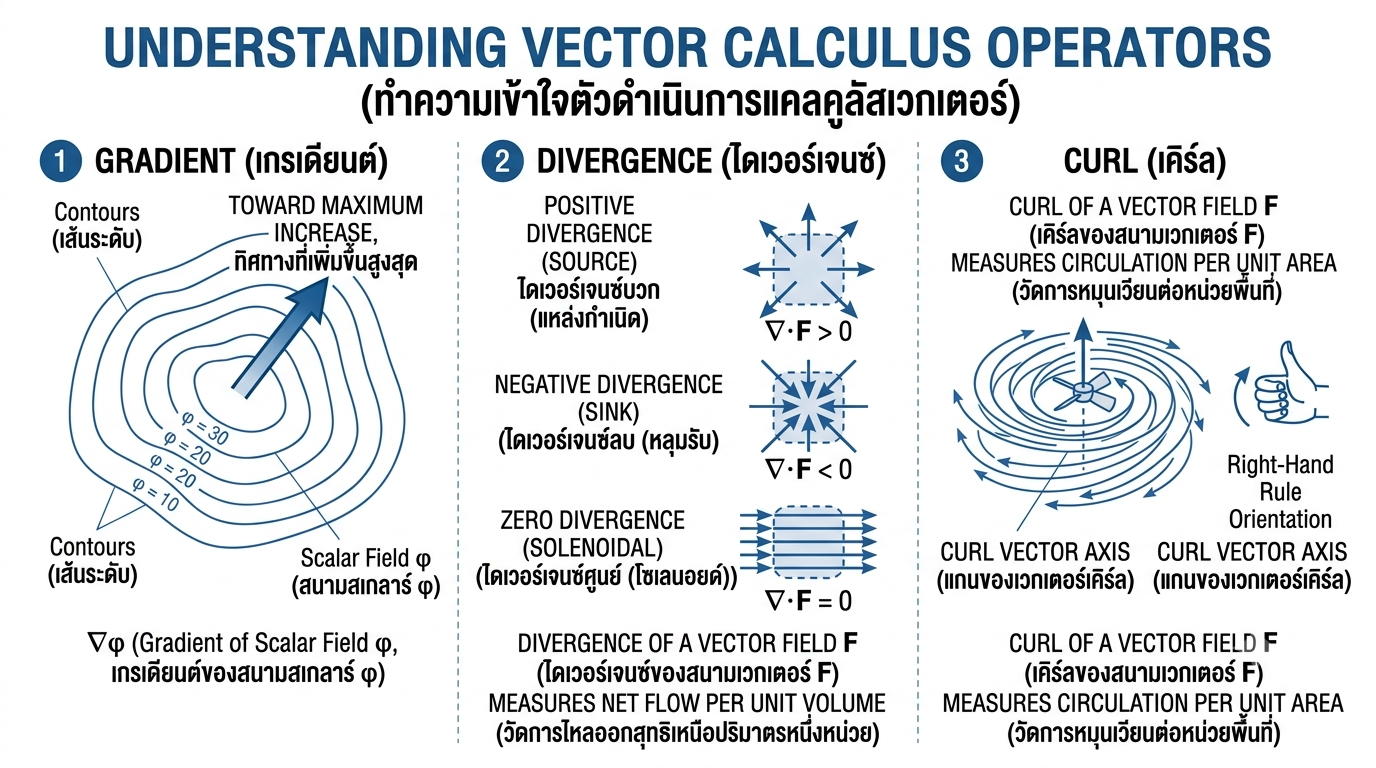
\includegraphics[width=0.8\textwidth]{images/chapter3/figure-06.png}
    \caption{ความหมายเชิงภาพของเกรเดียนต์ ไดเวอร์เจนซ์ และเคิร์ล}
\end{figure}

\paragraph{7.9.6 ตารางสรุป}

\begin{table}[htbp]
    \centering
    \begin{tabularx}{\textwidth}{L{0.18\textwidth} L{0.12\textwidth} L{0.14\textwidth} L{0.22\textwidth} Y}
        \hline
        \textbf{ตัวดำเนินการ} & \textbf{อินพุต} & \textbf{เอาต์พุต} & \textbf{ความหมาย} & \textbf{ตัวอย่างทางไฟฟ้า} \\
        \hline
        \(\nabla V\) & สเกลาร์ & เวกเตอร์ & ทิศเพิ่มเร็วที่สุด & \(\mathbf{E}=-\nabla V\) \\
        \(\nabla\cdot\mathbf{A}\) & เวกเตอร์ & สเกลาร์ & ฟลักซ์ออกสุทธิ & \(\nabla\cdot\mathbf{D}=\rho_v\) \\
        \(\nabla\times\mathbf{A}\) & เวกเตอร์ & เวกเตอร์ & การหมุนวนเฉพาะที่ & กฎฟาราเดย์/แอมแปร์--แมกซ์เวลล์ \\
        \(\nabla^2V\) & สเกลาร์ & สเกลาร์ & ความโค้งสุทธิ & สมการลาปลาซ/ปัวซอง \\
        \hline
    \end{tabularx}
\end{table}

\subsubsection{7.10 ทฤษฎีบทอินทิกรัลของสนาม}

\paragraph{7.10.1 ทฤษฎีบทไดเวอร์เจนซ์}

\[
\oint_S\mathbf{A}\cdot d\mathbf{S}
=\int_V(\nabla\cdot\mathbf{A})\,dV
\]

ฟลักซ์สุทธิที่ออกจากผิวปิดเท่ากับผลรวมความเป็นแหล่งกำเนิดในปริมาตร สนามและอนุพันธ์ต้องเรียบพอ หากมีจุดเอกฐานต้องจัดการอย่างระมัดระวัง

\paragraph{7.10.2 ทฤษฎีบทของสโตกส์}

\[
\oint_C\mathbf{A}\cdot d\mathbf{l}
=\int_S(\nabla\times\mathbf{A})\cdot d\mathbf{S}
\]

ทิศของ \(C\) ต้องสัมพันธ์กับเวกเตอร์ปกติของ \(S\) ตามกฎมือขวา การไหลเวียนรอบเส้นปิดเท่ากับฟลักซ์ของเคิร์ลผ่านพื้นผิว

% [รูปที่ 7: ความเชื่อมโยงรูปอินทิกรัลและรูปอนุพันธ์ของสนาม]
% ประเภทภาพ: Technical Illustration
% ตำแหน่งที่แนะนำ: หลังหัวข้อ 7.10.2
% วัตถุประสงค์การเรียนรู้: เชื่อมฟลักซ์กับไดเวอร์เจนซ์ และการไหลเวียนกับเคิร์ล
% คำอธิบายภาพ: ด้านซ้ายเป็นผิวปิดและแหล่งกำเนิดภายใน ด้านขวาเป็นพื้นผิวเปิด ขอบ $C$ และเวกเตอร์ปกติ
% องค์ประกอบที่ต้องมี: ผิว $S$ ปริมาตร $V$ เส้นขอบ $C$ เวกเตอร์ปกติ และกฎมือขวา
% ภาษาของป้ายกำกับ: ไทยและอังกฤษ
% สัดส่วนภาพ: 16:9
% Image Generation Prompt: Split engineering textbook diagram. Left: a closed surface S enclosing volume V, vector field arrows crossing outward and source symbols inside, labeled Divergence Theorem. Right: an open surface S bounded by curve C, circulation arrows around C, surface normal and right-hand-rule orientation, labeled Stokes' Theorem. White background, accurate blue technical line art, Thai-English labels, 16:9.
% Alt Text: ฟลักซ์ผ่านผิวปิดสัมพันธ์กับไดเวอร์เจนซ์ และการไหลเวียนสัมพันธ์กับเคิร์ล

\begin{figure}[htbp]
    \centering
    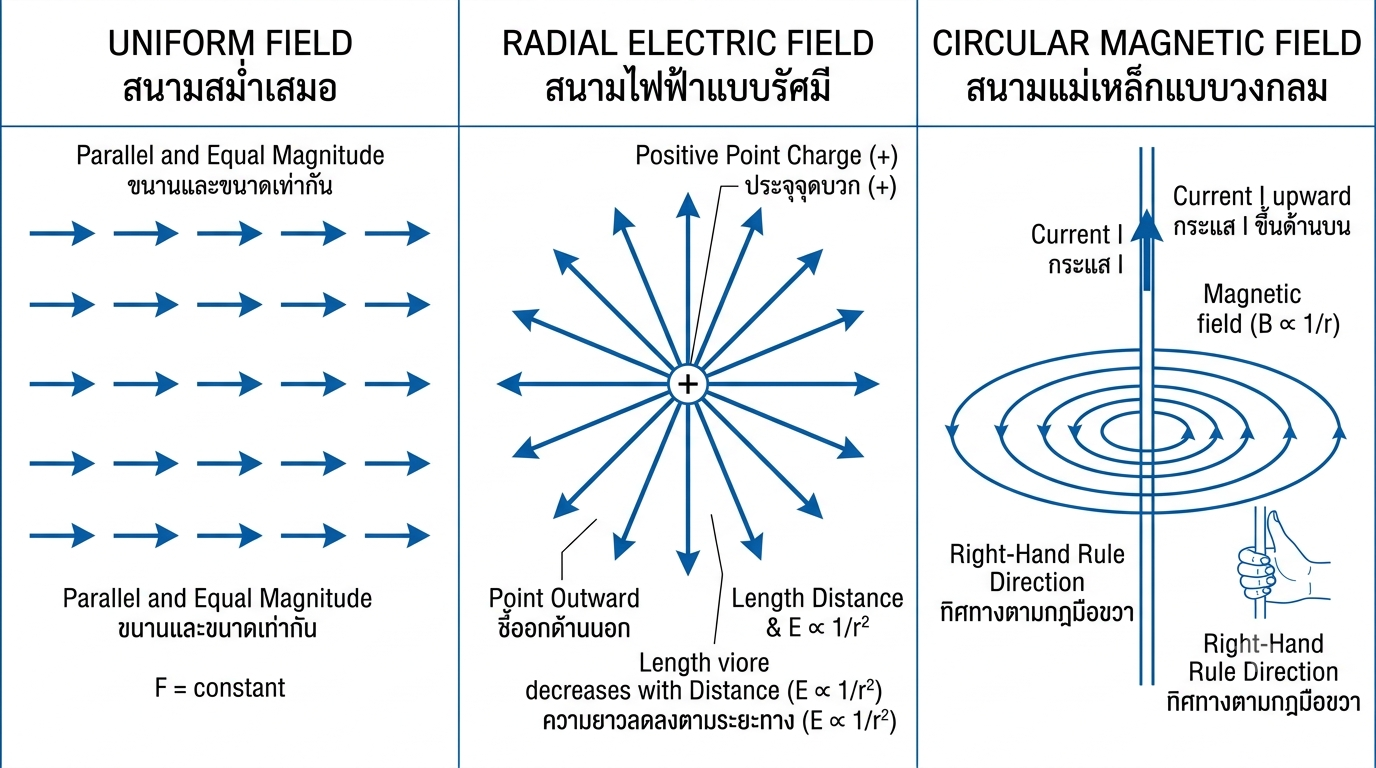
\includegraphics[width=0.8\textwidth]{images/chapter3/figure-07.png}
    \caption{ความเชื่อมโยงรูปอินทิกรัลและรูปอนุพันธ์ของสนาม}
\end{figure}

\subsubsection{7.11 แนวคิดเบื้องต้นของทฤษฎีสนามแม่เหล็กไฟฟ้า}

\paragraph{7.11.1 สนามไฟฟ้าจากประจุจุด}

ในสุญญากาศ สนามไฟฟ้าจากประจุจุด \(Q\) ที่จุดกำเนิดคือ

\[
\mathbf{E}=\frac{Q}{4\pi\varepsilon_0r^2}\mathbf{a}_r
\]

โดย \(Q\) หน่วย C, \(r\) หน่วย m, \(\varepsilon_0\approx8.854\times10^{-12}\) F/m และ \(\mathbf{a}_r\) ชี้ออกจากต้นกำเนิด หาก \(Q<0\) สนามชี้เข้า

\paragraph{7.11.2 หลักการซ้อนทับ}

สำหรับประจุหลายตัว

\[
\mathbf{E}_{\text{total}}=\sum_{i=1}^{N}\mathbf{E}_i
\]

หลักการซ้อนทับใช้เมื่อความสัมพันธ์ของระบบเป็นเชิงเส้นในช่วงที่พิจารณา

\paragraph{7.11.3 กฎของเกาส์}

รูปอินทิกรัล:

\[
\oint_S\mathbf{D}\cdot d\mathbf{S}=Q_{\text{enclosed}}
\]

รูปอนุพันธ์:

\[
\nabla\cdot\mathbf{D}=\rho_v
\]

กฎของเกาส์มีประสิทธิภาพสูงเมื่อมีสมมาตรทรงกลม ทรงกระบอก หรือระนาบชัดเจน ไม่ใช่เพียงเพราะเลือกผิวปิดใด ๆ แล้วจะคำนวณสนามได้ง่ายเสมอ

\paragraph{7.11.4 สนามแม่เหล็กรอบลวดตรงยาว}

สำหรับลวดตรงยาวมาก

\[
\mathbf{B}=\frac{\mu_0I}{2\pi\rho}\mathbf{a}_\phi
\]

โดย \(\mu_0=4\pi\times10^{-7}\) H/m และ \(\rho\) คือระยะตั้งฉากจากลวด ทิศ \(\mathbf{a}_\phi\) เป็นวงกลมรอบลวดตามกฎมือขวา

\paragraph{7.11.5 กฎของแอมแปร์ในกรณีสถิต}

\[
\oint_C\mathbf{H}\cdot d\mathbf{l}=I_{\text{enclosed}}
\]

ใช้ได้สะดวกเมื่อสมมาตรทำให้ \(\mathbf{H}\) สัมผัสเส้นทางและมีขนาดคงที่ตามส่วนสำคัญของเส้นทาง เช่น วงกลมรอบลวดตรงยาว

\paragraph{7.11.6 สมการแมกซ์เวลล์ในภาพรวม}

\begin{table}[htbp]
    \centering
    \begin{tabularx}{\textwidth}{L{0.20\textwidth} L{0.28\textwidth} Y}
        \hline
        \textbf{กฎ} & \textbf{รูปอนุพันธ์} & \textbf{ความหมายเชิงแนวคิด} \\
        \hline
        เกาส์สำหรับไฟฟ้า & \(\nabla\cdot\mathbf{D}=\rho_v\) & ประจุเป็นแหล่งของฟลักซ์ไฟฟ้า \\
        เกาส์สำหรับแม่เหล็ก & \(\nabla\cdot\mathbf{B}=0\) & ฟลักซ์แม่เหล็กผ่านผิวปิดสุทธิเป็นศูนย์ \\
        ฟาราเดย์ & \(\nabla\times\mathbf{E}=-\dfrac{\partial\mathbf{B}}{\partial t}\) & สนามแม่เหล็กที่เปลี่ยนตามเวลาสร้างสนามไฟฟ้าหมุนวน \\
        แอมแปร์--แมกซ์เวลล์ & \(\nabla\times\mathbf{H}=\mathbf{J}+\dfrac{\partial\mathbf{D}}{\partial t}\) & กระแสและสนามไฟฟ้าที่เปลี่ยนตามเวลาสร้างสนามแม่เหล็กหมุนวน \\
        \hline
    \end{tabularx}
\end{table}

บทนี้มุ่งอ่านความหมายของสมการผ่านแนวคิด grad--div--curl ยังไม่มุ่งแก้ปัญหาสนามแม่เหล็กไฟฟ้าเต็มรูปแบบ

\subsubsection{7.12 การประยุกต์เวกเตอร์กับสนามไฟฟ้า สนามแม่เหล็ก และแรง}

\paragraph{7.12.1 สนามไฟฟ้าจากประจุจุด}

ประจุ \(Q=5\) nC อยู่ที่จุดกำเนิด จงหาสนามที่ \(r=0.20\) m

\[
E=\frac{1}{4\pi\varepsilon_0}\frac{Q}{r^2}
\]

\[
E=(8.987\times10^9)\frac{5\times10^{-9}}{(0.20)^2}
\approx1.123\times10^3\ \text{V/m}
\]

\[
\boxed{\mathbf{E}\approx1.123\times10^3\mathbf{a}_r\ \text{V/m}}
\]

สนามชี้ออกเพราะประจุเป็นบวก และลดลงตาม \(1/r^2\)

\paragraph{7.12.2 แรงไฟฟ้าบนประจุ}

ถ้า \(q=2\ \mu\text{C}\) อยู่ในสนาม

\[
\mathbf{E}=(3\mathbf{a}_x-4\mathbf{a}_y)\ \text{kV/m}
\]

\[
\mathbf{F}=q\mathbf{E}
\]

\[
\boxed{\mathbf{F}=6\mathbf{a}_x-8\mathbf{a}_y\ \text{mN}}
\]

\[
|\mathbf{F}|=10\ \text{mN}
\]

\paragraph{7.12.3 แรงลอเรนซ์รวม}

\[
\mathbf{F}=q(\mathbf{E}+\mathbf{v}\times\mathbf{B})
\]

ส่วนไฟฟ้าสามารถทำงานและเปลี่ยนพลังงานจลน์ ส่วนแม่เหล็กตั้งฉากกับความเร็ว ณ ขณะนั้น จึงเปลี่ยนทิศแต่ไม่เปลี่ยนพลังงานจลน์ในกรณีสนามแม่เหล็กเพียงอย่างเดียว

\paragraph{ตัวอย่างที่ 9 แรงแม่เหล็กบนอิเล็กตรอน}

\[
\mathbf{v}=2.0\times10^6\mathbf{a}_x\ \text{m/s},\qquad
\mathbf{B}=0.20\mathbf{a}_z\ \text{T}
\]

สำหรับอิเล็กตรอน \(q=-1.602\times10^{-19}\) C

\[
\mathbf{v}\times\mathbf{B}
=-4.0\times10^5\mathbf{a}_y
\]

\[
\boxed{\mathbf{F}_m=6.408\times10^{-14}\mathbf{a}_y\ \text{N}}
\]

กฎมือขวาให้ทิศ \(\mathbf{v}\times\mathbf{B}\) สำหรับประจุบวก จึงต้องกลับทิศเมื่อเป็นอิเล็กตรอน

\paragraph{7.12.4 สนามแม่เหล็กรอบลวดตรง}

ลวดตรงมีกระแส \(I=10\) A ที่ระยะ \(\rho=0.05\) m

\[
B=\frac{\mu_0I}{2\pi\rho}
=4.0\times10^{-5}\ \text{T}
\]

\[
\boxed{\mathbf{B}=40\ \mu\text{T}\,\mathbf{a}_\phi}
\]

% [รูปที่ 8: ทิศแรงไฟฟ้าและแรงแม่เหล็กบนประจุและตัวนำ]
% ประเภทภาพ: Technical Illustration
% ตำแหน่งที่แนะนำ: หลังหัวข้อ 7.12.4
% วัตถุประสงค์การเรียนรู้: ฝึกอ่านทิศของ $q\mathbf{E}$, $q\mathbf{v}\times\mathbf{B}$ และ $I\mathbf{L}\times\mathbf{B}$
% คำอธิบายภาพ: สามส่วนแสดงประจุบวก/ลบในสนามไฟฟ้า ประจุเคลื่อนที่ในสนามแม่เหล็ก และตัวนำมีกระแสในสนามแม่เหล็ก
% องค์ประกอบที่ต้องมี: ลูกศร $\mathbf{E},\mathbf{v},\mathbf{B},\mathbf{F}$ กระแส $I$ และสัญลักษณ์จุด/กากบาท
% ภาษาของป้ายกำกับ: ไทยและอังกฤษ
% สัดส่วนภาพ: 16:9
% Image Generation Prompt: Three-panel engineering textbook illustration of force directions. Panel 1: positive and negative charges in a uniform electric field E, showing F=qE. Panel 2: moving charge with velocity v in magnetic field B, showing v cross B by right-hand rule and reversed force for a negative charge. Panel 3: current-carrying conductor with vector L in magnetic field B, showing F=I L cross B. Include x-y-z axes and dot/cross symbols. White background, blue technical style, Thai-English labels, 16:9.
% Alt Text: ทิศแรงไฟฟ้าและแรงแม่เหล็กด้วยกฎมือขวา

\begin{figure}[htbp]
    \centering
    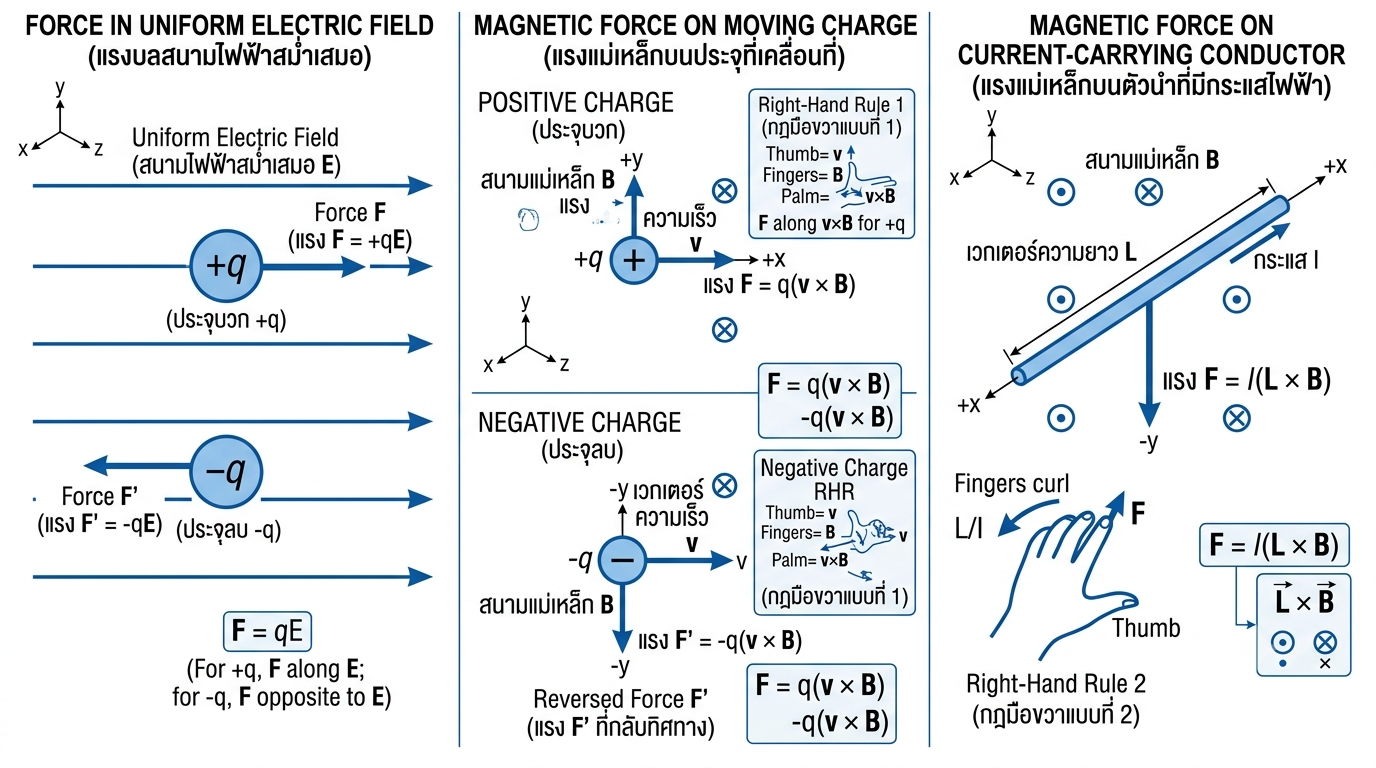
\includegraphics[width=0.8\textwidth]{images/chapter3/figure-08.png}
    \caption{ทิศแรงไฟฟ้าและแรงแม่เหล็กบนประจุและตัวนำ}
\end{figure}

\subsection{8. ความเข้าใจผิดที่พบบ่อย}

\subsubsection{8.1 เวกเตอร์ ``เป็นลบ''}

เวกเตอร์ตรงข้ามเขียนเป็น \(-\mathbf{A}\) มีขนาดเท่าเดิมและทิศกลับกัน องค์ประกอบบางแกนอาจติดลบตามทิศอ้างอิง แต่ขนาดเวกเตอร์ไม่เป็นลบ

\subsubsection{8.2 ขนาดเวกเตอร์เท่ากับผลบวกองค์ประกอบ}

ไม่ถูกต้อง ต้องใช้

\[
|\mathbf{A}|=\sqrt{A_x^2+A_y^2+A_z^2}
\]

\subsubsection{8.3 ดอตและครอสใช้แทนกันได้}

ดอตให้สเกลาร์และเลือกองค์ประกอบตามแนว ครอสให้เวกเตอร์ตั้งฉาก การเลือกผิดทำให้ชนิด หน่วย และความหมายของคำตอบผิด

\subsubsection{8.4 ครอสโปรดักต์สลับที่}

ไม่จริง

\[
\mathbf{A}\times\mathbf{B}=-(\mathbf{B}\times\mathbf{A})
\]

\subsubsection{8.5 ไดเวอร์เจนซ์เป็นเวกเตอร์}

ไดเวอร์เจนซ์ให้สเกลาร์ เคิร์ลให้เวกเตอร์ และเกรเดียนต์ของสเกลาร์ให้เวกเตอร์

\subsubsection{8.6 ไดเวอร์เจนซ์ศูนย์หมายถึงสนามศูนย์}

ไม่จริง สนามอาจมีค่าและหมุนวนได้โดยไม่มีฟลักซ์ออกสุทธิ

\subsubsection{8.7 เคิร์ลศูนย์ทำให้อินทิกรัลรอบเส้นปิดเป็นศูนย์เสมอ}

ต้องพิจารณาโดเมนและจุดเอกฐานด้วย หากบริเวณไม่เป็น simply connected อาจต้องวิเคราะห์เพิ่มเติม

\subsubsection{8.8 ฐานทรงกระบอกคงทิศ}

\(\mathbf{a}_\rho\) และ \(\mathbf{a}_\phi\) เปลี่ยนทิศตาม \(\phi\) จึงห้ามใช้กฎอนุพันธ์เหมือนฐานฉากโดยไม่ตรวจ scale factor

\subsubsection{8.9 สนามแม่เหล็กทำงานโดยตรงต่อประจุ}

เพราะ \(\mathbf{F}_m\perp\mathbf{v}\) จึงมี \(\mathbf{F}_m\cdot\mathbf{v}=0\) ในกรณีอุดมคติ สนามแม่เหล็กเปลี่ยนทิศความเร็วได้แต่ไม่เปลี่ยนพลังงานจลน์โดยตรง

\subsubsection{8.10 เส้นสนามเป็นวัตถุจริง}

เส้นสนามเป็นเครื่องมือแสดงทิศและขนาดสัมพัทธ์ ไม่ใช่วัตถุหรือเส้นทางบังคับของอนุภาคทุกกรณี

\subsection{9. การประยุกต์ใช้ในงานจริง}

\subsubsection{9.1 การออกแบบฉนวนและอิเล็กโทรด}

เกรเดียนต์ของศักย์ใช้ประเมินสนามไฟฟ้า บริเวณมุมแหลมหรือรัศมีโค้งเล็กอาจมีสนามเข้มสูง จึงต้องปรับรูปทรงและระยะฉนวนเพื่อลดความเสี่ยงการคายประจุ

\subsubsection{9.2 สายโคแอกเชียลและสายส่ง}

สมมาตรทรงกระบอกทำให้สนามไฟฟ้าอยู่ตาม \(\mathbf{a}_\rho\) และสนามแม่เหล็กอยู่ตาม \(\mathbf{a}_\phi\) การเลือกพิกัดที่เหมาะสมลดความซับซ้อนของสมการ

\subsubsection{9.3 มอเตอร์ไฟฟ้าและแอคชูเอเตอร์}

แรง \(I\mathbf{L}\times\mathbf{B}\) เป็นพื้นฐานของการสร้างแรงและแรงบิดในมอเตอร์ ลำโพง และขดลวดเคลื่อนที่

\subsubsection{9.4 เซนเซอร์ฮอลล์}

ค่าที่เซนเซอร์วัดได้สัมพันธ์กับองค์ประกอบของ \(\mathbf{B}\) ตามแกนไวรับ จึงตีความเป็นการฉายด้วยดอตโปรดักต์

\subsubsection{9.5 EMC และการเชื่อมโยงสนาม}

แนวคิดเคิร์ลช่วยอธิบายสนามที่เกิดจากกระแสเปลี่ยนตามเวลา การเหนี่ยวนำระหว่างลูป และเหตุผลที่ควรลดพื้นที่ลูปกระแสและออกแบบเส้นทางกระแสกลับ

\subsubsection{9.6 การวิเคราะห์เชิงตัวเลข}

เมื่อรูปทรงซับซ้อน วิศวกรใช้วิธี Finite Element หรือ Finite Difference แม้ซอฟต์แวร์จะคำนวณให้ ผู้ใช้ยังต้องเลือกพิกัด เงื่อนไขขอบเขต ตรวจหน่วย และตีความเวกเตอร์อย่างถูกต้อง

\subsection{10. กิจกรรมการเรียนรู้ระหว่างเรียน}

\subsubsection{กิจกรรมที่ 1: จำแนกปริมาณและอธิบายเหตุผล}

\begin{itemize}
\item \textbf{CLO:} CLO1
\item \textbf{เวลา:} 15 นาที
\item \textbf{รูปแบบ:} กลุ่ม 3--4 คน
\item \textbf{สื่อ:} บัตรคำ เช่น ศักย์ สนามไฟฟ้า พลังงาน ความหนาแน่นกระแส
\item \textbf{ขั้นตอน:} แบ่งบัตรเป็นสเกลาร์ เวกเตอร์ สนามสเกลาร์ และสนามเวกเตอร์ แล้วเขียนเหตุผลหนึ่งประโยค
\item \textbf{ผลที่คาดหวัง:} จำแนกจากจำนวนองค์ประกอบและการขึ้นกับตำแหน่ง
\item \textbf{ประเมิน:} ความถูกต้องและคุณภาพของเหตุผล
\end{itemize}

\subsubsection{กิจกรรมที่ 2: เลือกระบบพิกัดจากสมมาตร}

\begin{itemize}
\item \textbf{CLO:} CLO2
\item \textbf{เวลา:} 20 นาที
\item \textbf{รูปแบบ:} คู่
\item \textbf{สื่อ:} ภาพแผ่นขนาน ลวดตรง สายโคแอกเชียล ทรงกลม และอิเล็กโทรดซับซ้อน
\item \textbf{ขั้นตอน:} ระบุสมมาตร เลือกพิกัด และบอกว่าปริมาณน่าจะขึ้นกับตัวแปรใด
\item \textbf{ประเมิน:} เลือกพิกัดถูก ระบุตัวแปรถูก และอธิบายสมมาตรชัดเจน
\end{itemize}

\subsubsection{กิจกรรมที่ 3: คลินิกกฎมือขวา}

\begin{itemize}
\item \textbf{CLO:} CLO3, CLO5
\item \textbf{เวลา:} 20 นาที
\item \textbf{รูปแบบ:} รายบุคคลแล้วตรวจเป็นคู่
\item \textbf{ขั้นตอน:} วิเคราะห์ทิศครอสโปรดักต์ 4 กรณี และเพิ่มกรณีประจุลบ 2 กรณี
\item \textbf{ผลที่คาดหวัง:} ลดการสลับลำดับและการลืมกลับทิศสำหรับประจุลบ
\item \textbf{ประเมิน:} คำตอบพร้อมเหตุผลสั้น
\end{itemize}

\subsubsection{กิจกรรมที่ 4: วิเคราะห์ภาพสนามด้วย Grad--Div--Curl}

\begin{itemize}
\item \textbf{CLO:} CLO4
\item \textbf{เวลา:} 25 นาที
\item \textbf{รูปแบบ:} กลุ่ม
\item \textbf{ขั้นตอน:} ทำนายเครื่องหมายไดเวอร์เจนซ์ ทิศเคิร์ล สร้างฟังก์ชันอย่างง่าย และคำนวณตรวจสอบ
\item \textbf{ผลที่คาดหวัง:} เชื่อมภาพเชิงคุณภาพกับอนุพันธ์เชิงปริมาณ
\item \textbf{ประเมิน:} ความสอดคล้องระหว่างคำทำนาย ฟังก์ชัน และผลคำนวณ
\end{itemize}

\newpage

\subsection{11. กิจกรรมปฏิบัติการ}

\subsubsection{กิจกรรมปฏิบัติการที่ 1: การทำแผนที่ศักย์ไฟฟ้าบนกระดาษนำไฟฟ้า}

\paragraph{1. วัตถุประสงค์}

ผู้เรียนสามารถวัดศักย์ วาดเส้นศักย์เท่ากัน ประมาณสนามจาก \(\mathbf{E}=-\nabla V\) เปรียบเทียบรูปอิเล็กโทรด และอภิปรายความคลาดเคลื่อนได้

\paragraph{2. หลักการ}

ในแบบจำลองสองมิติ เส้นสนามตั้งฉากกับเส้นศักย์ และประมาณองค์ประกอบสนามได้ด้วย

\[
E_s\approx-\frac{\Delta V}{\Delta s}
\]

\paragraph{3. อุปกรณ์}

\begin{itemize}
\item แหล่งจ่าย DC 0--12 V ตั้งใช้งานไม่เกิน 10 V และจำกัดกระแส
\item กระดาษนำไฟฟ้าหรือชุดแผ่นนำไฟฟ้า
\item อิเล็กโทรดแผ่นขนานและจุด--แผ่น
\item ดิจิทัลมัลติมิเตอร์ความต้านทานอินพุตสูง
\item สายหุ้มฉนวน ไม้บรรทัด และกระดาษกราฟ
\item คอมพิวเตอร์พร้อม Python/MATLAB/Octave เป็นตัวเลือก
\end{itemize}

\paragraph{4. แผนภาพ}

% [รูปที่ 9: ชุดทดลองทำแผนที่ศักย์ไฟฟ้าบนกระดาษนำไฟฟ้า]
% ประเภทภาพ: Experimental Setup
% ตำแหน่งที่แนะนำ: หัวข้อกิจกรรมปฏิบัติการ ข้อ 4
% วัตถุประสงค์การเรียนรู้: แสดงการต่ออุปกรณ์แรงดันต่ำอย่างปลอดภัย
% คำอธิบายภาพ: แหล่งจ่าย 0–10 VDC ต่อกับอิเล็กโทรดบนแผ่นนำไฟฟ้า ขั้ว COM ต่อกับขั้วอ้างอิงและใช้โพรบวัดตามตาราง
% องค์ประกอบที่ต้องมี: แหล่งจ่ายจำกัดกระแส แผ่นนำไฟฟ้า มัลติมิเตอร์ โพรบ และเส้นศักย์ตัวอย่าง
% ภาษาของป้ายกำกับ: ไทยและอังกฤษ
% สัดส่วนภาพ: 16:9
% Image Generation Prompt: Safe educational laboratory setup for mapping electric potential on conductive paper. Show a current-limited 0–10 VDC supply connected to two electrodes on a gridded conductive sheet, digital multimeter COM connected to the zero-volt reference electrode, movable probe sampling grid points, example equipotential contours and electric-field arrows perpendicular to contours. White background, Thai-English labels, 16:9.
% Alt Text: ชุดทดลองแรงดันต่ำสำหรับวัดศักย์และประมาณสนามบนแผ่นนำไฟฟ้า

\begin{figure}[htbp]
    \centering
    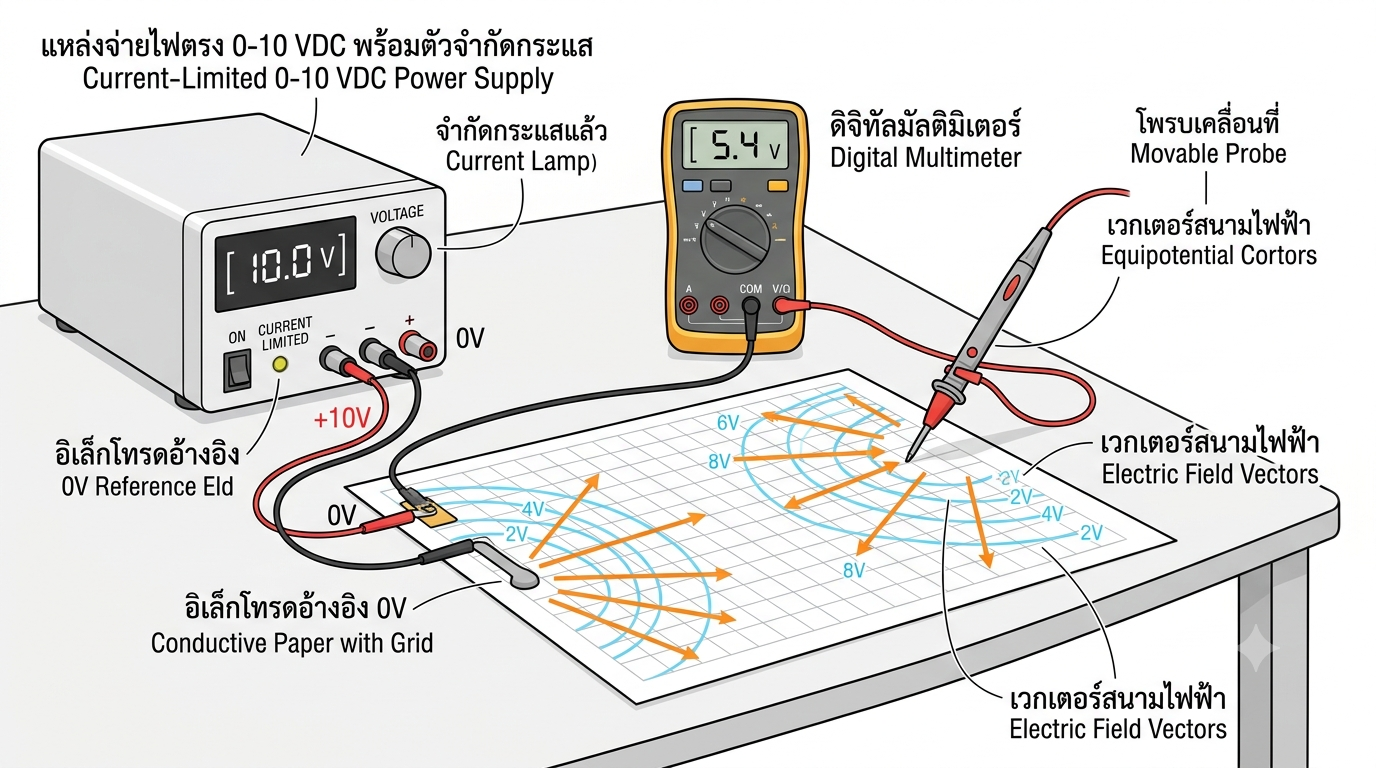
\includegraphics[width=0.8\textwidth]{images/chapter3/figure-09.png}
    \caption{ชุดทดลองทำแผนที่ศักย์ไฟฟ้าบนกระดาษนำไฟฟ้า}
\end{figure}

\paragraph{5. ความปลอดภัย}

\begin{enumerate}
\item ใช้แรงดันไม่เกิน 10 VDC และจำกัดกระแส
\item ปิดแหล่งจ่ายก่อนเปลี่ยนอิเล็กโทรดหรือสาย
\item ห้ามใช้ไฟบ้านหรือแหล่งจ่ายที่ไม่แยกทางไฟฟ้า
\item ตรวจฉนวนสายและรักษาพื้นที่ให้แห้ง
\item ไม่กดโพรบแรงจนแผ่นเสียหาย
\end{enumerate}

\paragraph{6. ขั้นตอน}

\begin{enumerate}
\item ตั้งแหล่งจ่ายเป็นศูนย์และปิดสวิตช์
\item ติดตั้งอิเล็กโทรดแผ่นขนานและต่อ 0 V กับ 10 V
\item ต่อ COM ของมัลติมิเตอร์กับขั้วอ้างอิง
\item วัดศักย์ตามจุดตารางโดยไม่แต่งค่าที่ไม่ได้วัด
\item ทำเครื่องหมายจุดใกล้ 2, 4, 6 และ 8 V แล้วลากเส้นศักย์
\item วาดลูกศรสนามตั้งฉากและชี้จากศักย์สูงไปต่ำ
\item ประมาณ \(|E|\approx|\Delta V/\Delta s|\) อย่างน้อยสามตำแหน่ง
\item ปิดแหล่งจ่าย เปลี่ยนเป็นอิเล็กโทรดจุด--แผ่น และทำซ้ำ
\item เปรียบเทียบสนามบริเวณกลาง ขอบ และใกล้ปลายแหลม
\end{enumerate}

\paragraph{7. ตารางบันทึกผล}

\begin{table}[htbp]
    \centering
    \begin{tabular}{l r r r r r l}
        \hline
        \textbf{รูปแบบอิเล็กโทรด} & \textbf{จุด \((x,y)\) cm} & \textbf{ศักย์ (V)} & \textbf{\(\Delta V\) (V)} & \textbf{\(\Delta s\) (m)} & \textbf{\(|E|\) (V/m)} & \textbf{หมายเหตุ} \\
        \hline
        แผ่นขนาน &  &  &  &  &  &  \\
        แผ่นขนาน &  &  &  &  &  &  \\
        จุด--แผ่น &  &  &  &  &  &  \\
        จุด--แผ่น &  &  &  &  &  &  \\
        \hline
    \end{tabular}
\end{table}

\paragraph{8. วิเคราะห์ผล}

\begin{itemize}
\item เส้นศักย์ใกล้กันหมายถึงขนาดสนามสูงกว่า
\item บริเวณกลางแผ่นขนานควรมีสนามค่อนข้างสม่ำเสมอ
\item บริเวณขอบเกิด fringing field
\item ใกล้ปลายแหลมเส้นศักย์มักหนาแน่น
\item ความคลาดเคลื่อนมาจากความต้านทานสัมผัส ความละเอียดตาราง ตำแหน่งโพรบ และความไม่สม่ำเสมอของแผ่น
\end{itemize}

\paragraph{9. คำถามหลังทดลอง}

\begin{enumerate}
\item เหตุใดเส้นสนามตั้งฉากกับเส้นศักย์
\item บริเวณใดมีสนามสูงสุด และข้อมูลใดสนับสนุน
\item รูปทรงอิเล็กโทรดมีผลอย่างไร
\item การกลับขั้วทำให้รูปและทิศสนามเปลี่ยนอย่างไร
\item แบบจำลองสองมิตินี้มีข้อจำกัดอะไร
\end{enumerate}

\paragraph{10. เกณฑ์ประเมิน}

\begin{table}[htbp]
    \centering
    \begin{tabularx}{0.76\textwidth}{Y r}
        \hline
        \textbf{ด้าน} & \textbf{สัดส่วน} \\
        \hline
        ความปลอดภัยและการต่ออุปกรณ์ & 20\% \\
        การบันทึกข้อมูลและหน่วย & 20\% \\
        แผนที่ศักย์ & 20\% \\
        การประมาณสนาม & 20\% \\
        การอภิปรายข้อจำกัดและความคลาดเคลื่อน & 20\% \\
        \hline
    \end{tabularx}
\end{table}

\subsection{12. การใช้ซอฟต์แวร์ โค้ด และการจำลอง}

\subsubsection{12.1 วัตถุประสงค์}

\begin{enumerate}
\item สร้างภาพสนามเวกเตอร์เพื่อช่วยตีความทิศและขนาด
\item สร้างเส้นชั้นศักย์และตรวจว่าทิศเกรเดียนต์ตั้งฉากกับเส้นชั้นค่า
\item คำนวณเชิงสัญลักษณ์ของเกรเดียนต์ ไดเวอร์เจนซ์ และเคิร์ล
\item เปรียบเทียบผลซอฟต์แวร์กับการคำนวณด้วยมือ
\item ตรวจจุดเอกฐาน โดเมน และข้อจำกัดของภาพที่สร้าง
\end{enumerate}

\subsubsection{12.2 เครื่องมือ}

\begin{itemize}
\item Python 3 พร้อม NumPy, Matplotlib และ SymPy
\item หรือ MATLAB/GNU Octave ที่มีคำสั่ง \texttt{meshgrid}, \texttt{quiver}, \texttt{contour}
\end{itemize}

ไม่รับรองความเข้ากันได้ทุกเวอร์ชัน ผู้เรียนควรตรวจเอกสารของรุ่นซอฟต์แวร์ที่ใช้

\subsubsection{12.3 Python: เส้นศักย์และสนามไฟฟ้า}

กำหนด

\[
V(x,y)=10-2x^2-y^2
\]

ดังนั้น

\[
\mathbf{E}=-\nabla V=4x\mathbf{a}_x+2y\mathbf{a}_y
\]

\begin{verbatim}
import numpy as np
import matplotlib.pyplot as plt

x = np.linspace(-2.0, 2.0, 21)
y = np.linspace(-2.0, 2.0, 21)
X, Y = np.meshgrid(x, y)

V = 10.0 - 2.0 * X**2 - Y**2
Ex = 4.0 * X
Ey = 2.0 * Y

magnitude = np.hypot(Ex, Ey)
nonzero = magnitude > 0

Ex_unit = np.zeros_like(Ex)
Ey_unit = np.zeros_like(Ey)
Ex_unit[nonzero] = Ex[nonzero] / magnitude[nonzero]
Ey_unit[nonzero] = Ey[nonzero] / magnitude[nonzero]

plt.figure(figsize=(9, 6))
contours = plt.contour(X, Y, V, levels=10)
plt.clabel(contours, inline=True, fontsize=8)
plt.quiver(X, Y, Ex_unit, Ey_unit, magnitude)
plt.xlabel("x (m)")
plt.ylabel("y (m)")
plt.title("Equipotential contours and electric-field direction")
plt.axis("equal")
plt.tight_layout()
plt.show()
\end{verbatim}

\paragraph{อธิบายโค้ด}

\begin{itemize}
\item \texttt{meshgrid} สร้างจุดตัวอย่างบนระนาบ
\item \texttt{contour} สร้างเส้นศักย์เท่ากัน
\item \texttt{quiver} แสดงลูกศรสนาม
\item normalization ใช้เปรียบเทียบทิศ ส่วน \texttt{magnitude} ใช้บอกความเข้มสัมพัทธ์
\item จุด \((0,0)\) มีสนามศูนย์ จึงต้องป้องกันการหารศูนย์
\end{itemize}

\paragraph{ผลที่ควรสังเกต}

\begin{enumerate}
\item ลูกศรสนามตั้งฉากกับเส้นศักย์
\item สนามชี้ไปทางศักย์ลดลง
\item ขนาดสนามเพิ่มเมื่อ \(|x|\) หรือ \(|y|\) เพิ่ม
\item การทำลูกศรให้ยาวเท่ากันช่วยดูทิศ แต่ไม่ควรตีความว่าแสดงขนาดจริง
\end{enumerate}

\subsubsection{12.4 SymPy: ตรวจ Grad--Div--Curl}

\begin{verbatim}
import sympy as sp

x, y, z = sp.symbols("x y z", real=True)

V = 10 - 2*x**2 - y**2 - 3*z
grad_V = sp.Matrix([
    sp.diff(V, x),
    sp.diff(V, y),
    sp.diff(V, z),
])

A = sp.Matrix([-y, x, 0])

div_A = (
    sp.diff(A[0], x)
    + sp.diff(A[1], y)
    + sp.diff(A[2], z)
)

curl_A = sp.Matrix([
    sp.diff(A[2], y) - sp.diff(A[1], z),
    sp.diff(A[0], z) - sp.diff(A[2], x),
    sp.diff(A[1], x) - sp.diff(A[0], y),
])

print("grad(V) =", grad_V)
print("div(A) =", sp.simplify(div_A))
print("curl(A) =", curl_A)
\end{verbatim}

ผลที่คาดหวัง:

\[
\nabla V=(-4x,-2y,-3)
\]

\[
\nabla\cdot\mathbf{A}=0
\]

\[
\nabla\times\mathbf{A}=(0,0,2)
\]

\subsubsection{12.5 MATLAB/GNU Octave}

\begin{verbatim}
[x, y] = meshgrid(linspace(-2, 2, 21), linspace(-2, 2, 21));

V  = 10 - 2*x.^2 - y.^2;
Ex = 4*x;
Ey = 2*y;

figure;
contour(x, y, V, 10);
hold on;
quiver(x, y, Ex, Ey);
axis equal;
xlabel('x (m)');
ylabel('y (m)');
title('Equipotential contours and electric field');
grid on;
\end{verbatim}

\subsubsection{12.6 งานมอบหมายซอฟต์แวร์}

ให้เลือกหนึ่งสนาม

\begin{enumerate}
\item \(\mathbf{A}=x\mathbf{a}_x+y\mathbf{a}_y\)
\item \(\mathbf{A}=-y\mathbf{a}_x+x\mathbf{a}_y\)
\item \(\mathbf{A}=\dfrac{x\mathbf{a}_x+y\mathbf{a}_y}{x^2+y^2}\) โดยตัดจุดกำเนิดออก
\end{enumerate}

ดำเนินการดังนี้

\begin{itemize}
\item สร้าง quiver plot
\item ทำนายไดเวอร์เจนซ์และเคิร์ลจากภาพ
\item คำนวณเชิงสัญลักษณ์
\item อธิบายความสอดคล้องระหว่างภาพกับผลคำนวณ
\item ระบุจุดเอกฐานและข้อจำกัดของโดเมน
\item เปลี่ยนช่วงแกนหรือความละเอียดกริด แล้วอธิบายผลต่อการมองเห็น
\end{itemize}

% [รูปที่ 10: ตัวอย่างเส้นศักย์และสนามไฟฟ้าจากซอฟต์แวร์]
% ประเภทภาพ: Graph
% ตำแหน่งที่แนะนำ: หลังหัวข้อ 12.6
% วัตถุประสงค์การเรียนรู้: แสดงความตั้งฉากระหว่างเส้นศักย์กับสนาม
% คำอธิบายภาพ: กราฟระนาบ $xy$ มี contour ของ $V=10-2x^2-y^2$ และลูกศร $\mathbf{E}=(4x,2y)$
% องค์ประกอบที่ต้องมี: แกนพร้อมหน่วย เส้น contour มีค่ากำกับ ลูกศรสนาม และ colorbar ขนาดสนาม
% ภาษาของป้ายกำกับ: ไทยและอังกฤษ
% สัดส่วนภาพ: 4:3
% Graph Generation Prompt: Plot V(x,y)=10-2x^2-y^2 over -2<=x<=2 and -2<=y<=2 with labeled contour lines. Overlay E=-grad(V)=(4x,2y) using quiver arrows. Use equal axis scaling, axes in meters, a colorbar for field magnitude, and clearly show arrows normal to equipotential contours. Academic engineering graph, white background.
% Alt Text: เส้นศักย์รูปวงรีและลูกศรสนามไฟฟ้าที่ตั้งฉากกับเส้นศักย์

\begin{figure}[htbp]
    \centering
    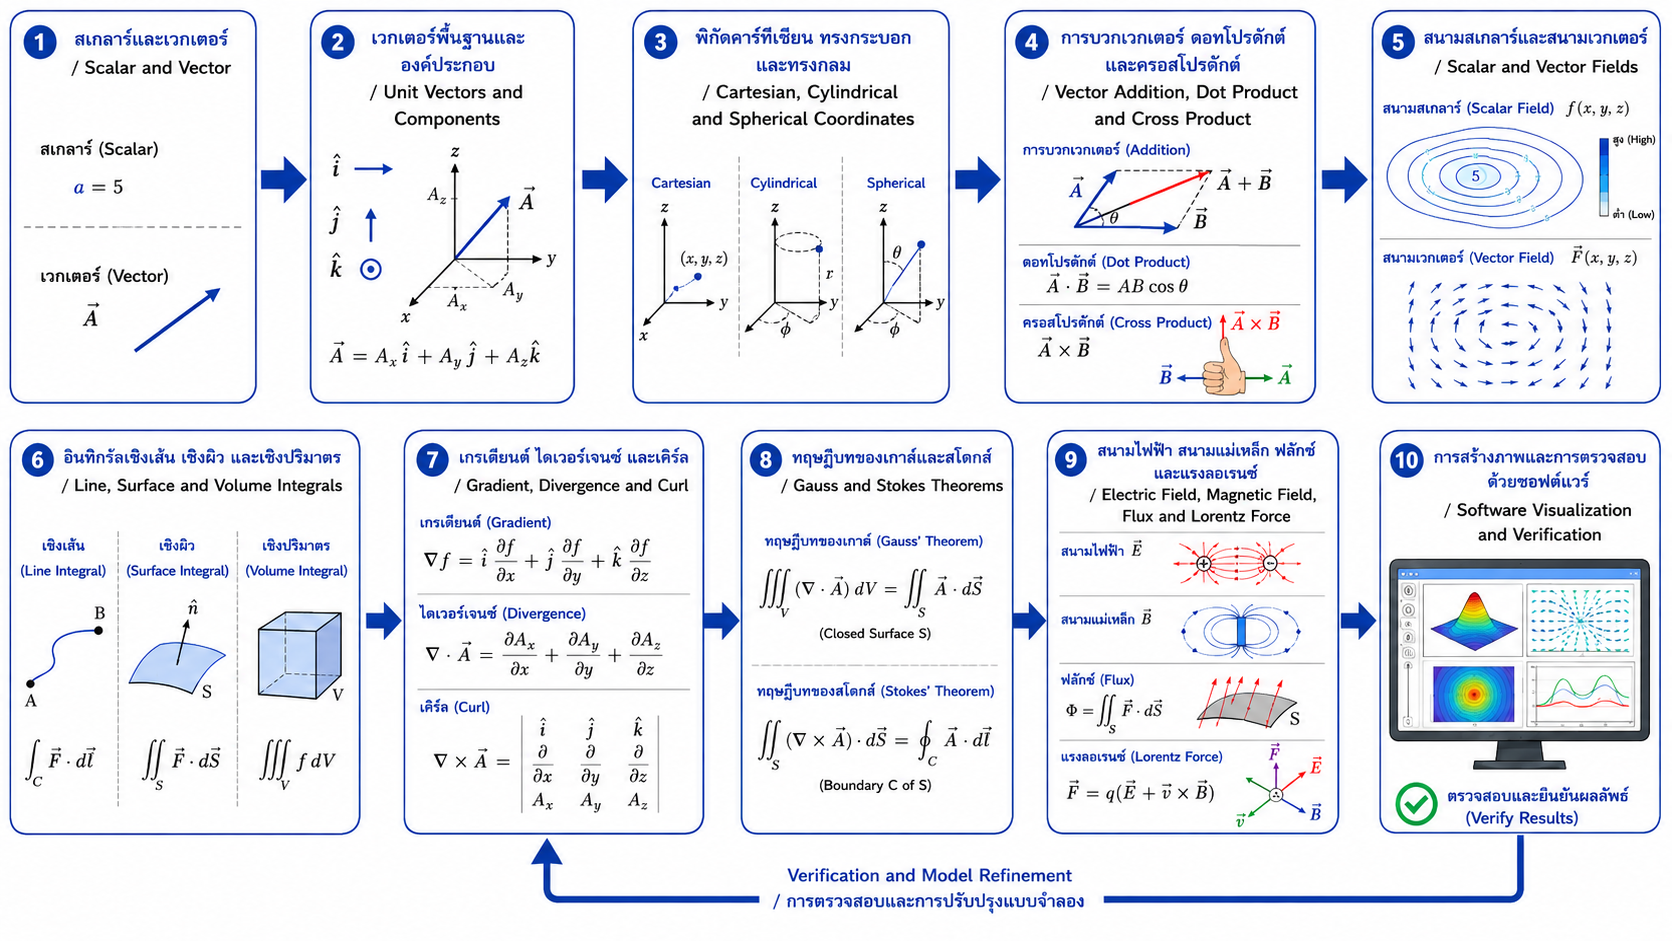
\includegraphics[width=0.8\textwidth]{images/chapter3/figure-01.png}
    \caption{ตัวอย่างเส้นศักย์และสนามไฟฟ้าจากซอฟต์แวร์}
\end{figure}

\subsubsection{12.7 ข้อผิดพลาดที่พบบ่อยในการใช้ซอฟต์แวร์}

\begin{itemize}
\item ลืมเครื่องหมายลบใน \(\mathbf{E}=-\nabla V\)
\item ลืมใช้ \texttt{.*}, \texttt{.\^{}} ใน MATLAB/Octave สำหรับข้อมูลแบบอาร์เรย์
\item กริดหยาบเกินไปจนภาพไม่สะท้อนลักษณะสนาม
\item สเกลแกนไม่เท่ากัน ทำให้ทิศดูบิดเบือน
\item ใช้ normalization แล้วตีความขนาดผิด
\item รวมจุดเอกฐานไว้ในกริด ทำให้เกิด \texttt{inf} หรือ \texttt{nan}
\item เชื่อผลซอฟต์แวร์โดยไม่ตรวจหน่วยและกรณีง่ายด้วยมือ
\end{itemize}

\subsection{13. สรุปท้ายบท}

\begin{enumerate}
\item สเกลาร์มีขนาด ส่วนเวกเตอร์มีทั้งขนาดและทิศทาง
\item เวกเตอร์เขียนเป็นองค์ประกอบตามเวกเตอร์หนึ่งหน่วย และขนาดหาได้จากผลบวกกำลังสองขององค์ประกอบ
\item พิกัดฉากเหมาะกับสมมาตรตามระนาบ พิกัดทรงกระบอกเหมาะกับสมมาตรรอบแกน และพิกัดทรงกลมเหมาะกับสมมาตรรอบจุด
\item ดอตโปรดักต์ให้สเกลาร์ ใช้กับการฉาย งาน และฟลักซ์
\item ครอสโปรดักต์ให้เวกเตอร์ตั้งฉาก ใช้กับพื้นที่ แรงแม่เหล็ก และแรงบนตัวนำ
\item สนามสเกลาร์ให้ค่าหนึ่งค่าต่อจุด ส่วนสนามเวกเตอร์ให้เวกเตอร์ต่อจุด
\item เกรเดียนต์ชี้ไปทางเพิ่มเร็วที่สุด และ \(\mathbf{E}=-\nabla V\)
\item ไดเวอร์เจนซ์บอกการแผ่ออกสุทธิ ส่วนเคิร์ลบอกการหมุนวนเฉพาะที่
\item ทฤษฎีบทไดเวอร์เจนซ์เชื่อมฟลักซ์ผ่านผิวปิดกับแหล่งกำเนิดในปริมาตร
\item ทฤษฎีบทสโตกส์เชื่อมการไหลเวียนรอบเส้นขอบกับเคิร์ลผ่านพื้นผิว
\item กฎสนามแม่เหล็กไฟฟ้าใช้ภาษาเวกเตอร์เพื่อเชื่อมประจุ กระแส สนาม และการเปลี่ยนตามเวลา
\item ซอฟต์แวร์ช่วยสร้างภาพและตรวจผล แต่ผู้เรียนต้องตรวจสมมาตร หน่วย ทิศ โดเมน และจุดเอกฐาน
\end{enumerate}

\subsubsection{13.1 ตารางสมการสำคัญ}

\begin{table}[htbp]
    \centering
    \begin{tabular}{l l}
        \hline
        \textbf{หัวข้อ} & \textbf{สมการ} \\
        \hline
        ขนาดเวกเตอร์ & \(|\mathbf{A}|=\sqrt{A_x^2+A_y^2+A_z^2}\) \\
        เวกเตอร์หนึ่งหน่วย & \(\mathbf{a}_A=\mathbf{A}/|\mathbf{A}|\) \\
        ดอตโปรดักต์ & \(\mathbf{A}\cdot\mathbf{B}=|\mathbf{A}||\mathbf{B}|\cos\theta\) \\
        ครอสโปรดักต์ & \(\mathbf{A}\times\mathbf{B}=|\mathbf{A}||\mathbf{B}|\sin\theta\,\mathbf{a}_n\) \\
        งาน & \(W=\int_C\mathbf{F}\cdot d\mathbf{l}\) \\
        ฟลักซ์ & \(\Phi=\int_S\mathbf{A}\cdot d\mathbf{S}\) \\
        สนามไฟฟ้าจากศักย์ & \(\mathbf{E}=-\nabla V\) \\
        ไดเวอร์เจนซ์ & \(\nabla\cdot\mathbf{A}\) \\
        เคิร์ล & \(\nabla\times\mathbf{A}\) \\
        ทฤษฎีบทไดเวอร์เจนซ์ & \(\oint_S\mathbf{A}\cdot d\mathbf{S}=\int_V\nabla\cdot\mathbf{A}\,dV\) \\
        ทฤษฎีบทสโตกส์ & \(\oint_C\mathbf{A}\cdot d\mathbf{l}=\int_S(\nabla\times\mathbf{A})\cdot d\mathbf{S}\) \\
        แรงลอเรนซ์ & \(\mathbf{F}=q(\mathbf{E}+\mathbf{v}\times\mathbf{B})\) \\
        แรงบนตัวนำ & \(\mathbf{F}=I\mathbf{L}\times\mathbf{B}\) \\
        \hline
    \end{tabular}
\end{table}

\subsection{14. คำถามทบทวน}

\begin{enumerate}
\item เพราะเหตุใดสนามไฟฟ้าจึงเป็นเวกเตอร์ แต่ศักย์ไฟฟ้าเป็นสเกลาร์
\item การเลือกระบบพิกัดจากสมมาตรช่วยลดความซับซ้อนอย่างไร
\item เปรียบเทียบดอตโปรดักต์กับครอสโปรดักต์ทั้งชนิดผลลัพธ์และการใช้งาน
\item เหตุใดสนามไฟฟ้าสถิตตั้งฉากกับพื้นผิวศักย์เท่ากัน
\item ไดเวอร์เจนซ์เป็นศูนย์บอกอะไรและไม่ได้บอกอะไร
\item เคิร์ลสัมพันธ์กับทฤษฎีบทสโตกส์อย่างไร
\item เหตุใดแรงแม่เหล็กเพียงอย่างเดียวไม่เปลี่ยนพลังงานจลน์ของประจุ
\item เปรียบเทียบกฎของเกาส์รูปอินทิกรัลกับรูปอนุพันธ์
\item จุดเอกฐานมีผลต่อการใช้ตัวดำเนินการเวกเตอร์อย่างไร
\item การสร้างภาพด้วยซอฟต์แวร์มีประโยชน์และข้อจำกัดอะไร
\end{enumerate}

\subsection{15. แบบฝึกหัดท้ายบท}

\subsubsection{15.1 ระดับพื้นฐาน}

\begin{enumerate}
\item จำแนกปริมาณต่อไปนี้เป็นสเกลาร์หรือเวกเตอร์: ศักย์ไฟฟ้า พลังงาน สนามไฟฟ้า ความหนาแน่นกระแส และกำลังไฟฟ้า
\item ให้ \(\mathbf{A}=4\mathbf{a}_x-3\mathbf{a}_y+12\mathbf{a}_z\) จงหาขนาดและเวกเตอร์หนึ่งหน่วย
\item จุด \(P=(6,-8,3)\) จงแปลงเป็นพิกัดทรงกระบอก โดยใช้มุมช่วง \(0^\circ\) ถึง \(360^\circ\)
\item ให้ \(\mathbf{A}=2\mathbf{a}_x+3\mathbf{a}_y-\mathbf{a}_z\) และ \(\mathbf{B}=-\mathbf{a}_x+4\mathbf{a}_y+2\mathbf{a}_z\) จงหา \(\mathbf{A}+\mathbf{B}\) และ \(\mathbf{A}-\mathbf{B}\)
\item ให้ \(\mathbf{A}=3\mathbf{a}_x+4\mathbf{a}_y\) และ \(\mathbf{B}=4\mathbf{a}_x-3\mathbf{a}_y\) จงหา \(\mathbf{A}\cdot\mathbf{B}\) และมุมระหว่างเวกเตอร์
\end{enumerate}

\subsubsection{15.2 ระดับวิเคราะห์}

\begin{enumerate}
\setcounter{enumi}{5}
\item ให้ \(P_1=(1,-2,3)\) และ \(P_2=(5,1,-1)\) จงหาเวกเตอร์ ระยะทาง และเวกเตอร์หนึ่งหน่วยจาก \(P_1\) ไป \(P_2\)
\item ให้ \(\mathbf{A}=2\mathbf{a}_x-\mathbf{a}_y+2\mathbf{a}_z\) และ \(\mathbf{B}=\mathbf{a}_x+2\mathbf{a}_y-2\mathbf{a}_z\) จงหามุมระหว่างเวกเตอร์
\item หา \(\mathbf{A}\times\mathbf{B}\) เมื่อ \(\mathbf{A}=\mathbf{a}_x+2\mathbf{a}_y+3\mathbf{a}_z\) และ \(\mathbf{B}=2\mathbf{a}_x-\mathbf{a}_y+\mathbf{a}_z\) แล้วตรวจว่าผลลัพธ์ตั้งฉากกับทั้งสองเวกเตอร์
\item ให้ \(V=5x^2-2xy+z^2\) V จงหา \(\nabla V\) และ \(\mathbf{E}\) ที่ \((1,2,-1)\)
\item ให้ \(\mathbf{A}=xy\mathbf{a}_x+yz\mathbf{a}_y+zx\mathbf{a}_z\) จงหาไดเวอร์เจนซ์ที่ \((1,2,3)\)
\item ให้ \(\mathbf{A}=z\mathbf{a}_x+x\mathbf{a}_y+y\mathbf{a}_z\) จงหาเคิร์ล
\item ให้ \(\mathbf{F}=2x\mathbf{a}_x+2y\mathbf{a}_y\) N จงหางานจาก \((0,0)\) ไป \((2,1)\) และอธิบายว่าเหตุใดไม่ขึ้นกับเส้นทาง
\item สนามสม่ำเสมอ \(\mathbf{A}=5\mathbf{a}_z\) ผ่านพื้นผิวพื้นที่ \(0.20\) m\(^2\) ซึ่งเวกเตอร์ปกติทำมุม \(60^\circ\) กับ \(+z\) จงหาฟลักซ์
\end{enumerate}

\subsubsection{15.3 ระดับประยุกต์ใช้}

\begin{enumerate}
\setcounter{enumi}{13}
\item ประจุ \(q=3\ \mu\)C เคลื่อนที่ด้วย \(\mathbf{v}=2\times10^5\mathbf{a}_x\) m/s ใน \(\mathbf{E}=2\times10^3\mathbf{a}_y\) V/m และ \(\mathbf{B}=0.10\mathbf{a}_z\) T จงหาแรงลอเรนซ์รวม
\item ตัวนำยาว \(0.25\) m วางตาม \(\mathbf{a}_L=(3\mathbf{a}_x+4\mathbf{a}_y)/5\) มีกระแส \(8\) A ใน \(\mathbf{B}=0.50\mathbf{a}_z\) T จงหาแรง
\item ประจุ \(Q=8\) nC อยู่ที่ \(P_Q=(1,0,0)\) m จงหาสนามที่ \(P=(1,3,4)\) m ในสุญญากาศ
\item ให้ \(\mathbf{D}=4\rho\,\mathbf{a}_\rho\) nC/m\(^2\) ในทรงกระบอกรัศมี \(0.10\) m และยาว \(0.50\) m จงหาฟลักซ์ผ่านผิวด้านข้าง และอธิบายว่าผิวหัว--ท้ายมีส่วนหรือไม่
\item ออกแบบขั้นตอนเชิงคำนวณเพื่อประเมินสนามไฟฟ้าจากข้อมูลศักย์บนกริดสองมิติ ระบุวิธีประมาณอนุพันธ์ การจัดการขอบเขต และวิธีตรวจสอบผล
\end{enumerate}

\subsection{16. แนวคำตอบและเฉลยสำหรับผู้สอน}

\subsubsection{16.1 ระดับพื้นฐาน}

\paragraph{ข้อ 1}

ศักย์ไฟฟ้า พลังงาน และกำลังเป็นสเกลาร์; สนามไฟฟ้าและความหนาแน่นกระแสเป็นเวกเตอร์

\paragraph{ข้อ 2}

\[
|\mathbf{A}|=\sqrt{16+9+144}=13
\]

\[
\boxed{\mathbf{a}_A=\frac{4}{13}\mathbf{a}_x-\frac{3}{13}\mathbf{a}_y+\frac{12}{13}\mathbf{a}_z}
\]

\paragraph{ข้อ 3}

\[
\rho=\sqrt{6^2+(-8)^2}=10
\]

จุดอยู่ควอดแรนต์ที่ 4

\[
\phi=360^\circ-\tan^{-1}(8/6)=306.87^\circ
\]

\[
\boxed{(\rho,\phi,z)=(10,306.87^\circ,3)}
\]

\paragraph{ข้อ 4}

\[
\boxed{\mathbf{A}+\mathbf{B}=\mathbf{a}_x+7\mathbf{a}_y+\mathbf{a}_z}
\]

\[
\boxed{\mathbf{A}-\mathbf{B}=3\mathbf{a}_x-\mathbf{a}_y-3\mathbf{a}_z}
\]

\paragraph{ข้อ 5}

\[
\mathbf{A}\cdot\mathbf{B}=12-12=0
\]

\[
\boxed{\theta=90^\circ}
\]

\subsubsection{16.2 ระดับวิเคราะห์}

\paragraph{ข้อ 6}

\[
\mathbf{R}_{12}=4\mathbf{a}_x+3\mathbf{a}_y-4\mathbf{a}_z
\]

\[
R_{12}=\sqrt{41}\ \text{m}
\]

\[
\boxed{\mathbf{a}_{12}=\frac{4\mathbf{a}_x+3\mathbf{a}_y-4\mathbf{a}_z}{\sqrt{41}}}
\]

\paragraph{ข้อ 7}

\[
\mathbf{A}\cdot\mathbf{B}=-4,\qquad |\mathbf{A}|=|\mathbf{B}|=3
\]

\[
\boxed{\theta=\cos^{-1}(-4/9)\approx116.39^\circ}
\]

\paragraph{ข้อ 8}

\[
\boxed{\mathbf{A}\times\mathbf{B}=5\mathbf{a}_x+5\mathbf{a}_y-5\mathbf{a}_z}
\]

ตรวจสอบ:

\[
(\mathbf{A}\times\mathbf{B})\cdot\mathbf{A}=0
\]

\[
(\mathbf{A}\times\mathbf{B})\cdot\mathbf{B}=0
\]

\paragraph{ข้อ 9}

\[
\nabla V=(10x-2y)\mathbf{a}_x-2x\mathbf{a}_y+2z\mathbf{a}_z
\]

\[
\mathbf{E}=-\nabla V
\]

ที่ \((1,2,-1)\)

\[
\boxed{\mathbf{E}=-6\mathbf{a}_x+2\mathbf{a}_y+2\mathbf{a}_z\ \text{V/m}}
\]

\paragraph{ข้อ 10}

\[
\nabla\cdot\mathbf{A}=y+z+x
\]

ที่ \((1,2,3)\)

\[
\boxed{\nabla\cdot\mathbf{A}=6}
\]

\paragraph{ข้อ 11}

\[
\boxed{\nabla\times\mathbf{A}=\mathbf{a}_x+\mathbf{a}_y+\mathbf{a}_z}
\]

\paragraph{ข้อ 12}

สนามเป็นเกรเดียนต์ของ \(\psi=x^2+y^2\)

\[
W=\psi(2,1)-\psi(0,0)=5\ \text{J}
\]

\[
\boxed{W=5\ \text{J}}
\]

และ \(\nabla\times\mathbf{F}=\mathbf{0}\) ในโดเมนทั่วระนาบ จึงไม่ขึ้นกับเส้นทาง

\paragraph{ข้อ 13}

\[
\Phi=AS\cos\theta=(5)(0.20)\cos60^\circ
\]

\[
\boxed{\Phi=0.50\ \text{หน่วยสนาม}\cdot\text{m}^2}
\]

\subsubsection{16.3 ระดับประยุกต์ใช้}

\paragraph{ข้อ 14}

\[
\mathbf{v}\times\mathbf{B}
=(2\times10^5\mathbf{a}_x)\times(0.10\mathbf{a}_z)
=-2\times10^4\mathbf{a}_y
\]

\[
\mathbf{E}+\mathbf{v}\times\mathbf{B}
=-1.8\times10^4\mathbf{a}_y
\]

\[
\boxed{\mathbf{F}=-5.4\times10^{-2}\mathbf{a}_y\ \text{N}}
\]

\paragraph{ข้อ 15}

\[
\mathbf{L}=0.25\left(\frac{3}{5}\mathbf{a}_x+\frac{4}{5}\mathbf{a}_y\right)
=0.15\mathbf{a}_x+0.20\mathbf{a}_y
\]

\[
\boxed{\mathbf{F}=0.80\mathbf{a}_x-0.60\mathbf{a}_y\ \text{N}}
\]

\[
|\mathbf{F}|=1.0\ \text{N}
\]

\paragraph{ข้อ 16}

\[
\mathbf{R}=3\mathbf{a}_y+4\mathbf{a}_z,\quad
R=5,\quad
\mathbf{a}_R=\frac{3}{5}\mathbf{a}_y+\frac{4}{5}\mathbf{a}_z
\]

\[
E=(8.987\times10^9)\frac{8\times10^{-9}}{25}
=2.876\ \text{V/m}
\]

\[
\boxed{\mathbf{E}=1.726\mathbf{a}_y+2.301\mathbf{a}_z\ \text{V/m}}
\]

\paragraph{ข้อ 17}

บนผิวด้านข้าง \(\rho=0.10\) m และ

\[
d\mathbf{S}=\mathbf{a}_\rho\,\rho\,d\phi\,dz
\]

\[
\Phi=\int_0^{0.5}\int_0^{2\pi}
(4\rho)\rho\,d\phi\,dz\ \text{nC}
\]

ที่ \(\rho=0.10\)

\[
\Phi=4(0.10)^2(2\pi)(0.50)=0.04\pi\ \text{nC}
\]

\[
\boxed{\Phi\approx0.1257\ \text{nC}}
\]

ผิวหัว--ท้ายมีเวกเตอร์ปกติตาม \(\pm\mathbf{a}_z\) แต่ \(\mathbf{D}\) อยู่ตาม \(\mathbf{a}_\rho\) จึงมีดอตโปรดักต์เป็นศูนย์

\paragraph{ข้อ 18}

แนวคำตอบ:

\begin{enumerate}
\item จัดข้อมูลเป็นตาราง \(V_{i,j}\) และกำหนดระยะกริด \(\Delta x,\Delta y\)
\item จุดภายในใช้ central difference
\end{enumerate}

\[
E_x\approx-\frac{V_{i+1,j}-V_{i-1,j}}{2\Delta x}
\]

\[
E_y\approx-\frac{V_{i,j+1}-V_{i,j-1}}{2\Delta y}
\]

\begin{enumerate}
\setcounter{enumi}{2}
\item จุดขอบใช้ forward/backward difference หรือใช้เงื่อนไขขอบเขตที่ทราบ
\item สร้าง contour ของ \(V\) และ quiver ของ \(\mathbf{E}\)
\item ตรวจว่าลูกศรตั้งฉากกับ contour และชี้จากศักย์สูงไปต่ำ
\item ตรวจกรณีทดสอบที่ทราบคำตอบ เช่น \(V=-E_0x\)
\item วิเคราะห์ผลของความละเอียดกริดและ noise ต่ออนุพันธ์
\end{enumerate}

\subsection{17. ข้อเสนอแนะสำหรับผู้สอน}

\subsubsection{17.1 ลำดับการสอน}

\textbf{สัปดาห์ที่ 4}

\begin{enumerate}
\item เปิดด้วยสนามไฟฟ้าและแรงแม่เหล็ก
\item ทบทวนสเกลาร์ เวกเตอร์ ขนาด และเวกเตอร์หนึ่งหน่วย
\item สอนพิกัดผ่านสมมาตรของอุปกรณ์
\item ฝึกบวก ลบ ดอต และครอส
\item ใช้กิจกรรมจำแนกปริมาณและกฎมือขวา
\end{enumerate}

\textbf{สัปดาห์ที่ 5}

\begin{enumerate}
\item เชื่อมสนามสเกลาร์กับเส้นศักย์
\item อธิบายอินทิกรัลเส้นและฟลักซ์
\item ใช้ภาพก่อนสูตร grad--div--curl
\item เชื่อมทฤษฎีบทไดเวอร์เจนซ์และสโตกส์กับกฎสนาม
\item ปิดบทด้วยซอฟต์แวร์หรือการทำแผนที่ศักย์
\end{enumerate}

\subsubsection{17.2 จุดที่มักมีปัญหา}

\begin{itemize}
\item สลับ \(\theta\) และ \(\phi\)
\item ใช้ \(\tan^{-1}(y/x)\) โดยไม่พิจารณาควอดแรนต์
\item ลืมว่าฐานพิกัดโค้งเปลี่ยนตามตำแหน่ง
\item สลับลำดับครอสโปรดักต์
\item หาอนุพันธ์ย่อยผิด
\item จำสูตรโดยไม่แยกชนิดอินพุต--เอาต์พุต
\item ลืมเครื่องหมายลบของ \(\mathbf{E}=-\nabla V\)
\item ไม่ตรวจหน่วย
\item ใช้กฎของเกาส์หรือแอมแปร์โดยสมมาตรไม่พอ
\end{itemize}

\subsubsection{17.3 กลยุทธ์}

\begin{enumerate}
\item ให้ผู้เรียนทำนายทิศก่อนหาขนาด
\item ใช้สีแยกสเกลาร์ เวกเตอร์ และตัวดำเนินการ
\item เชื่อมทุกสูตรกับรูปทางเรขาคณิต
\item สลับการคำนวณมือกับภาพสนาม
\item ให้คะแนนการตีความหน่วยและทิศ
\item ใช้ Exit Ticket เช่น ``divergence = 0 แต่ curl ไม่เป็นศูนย์เป็นไปได้หรือไม่''
\end{enumerate}

\subsubsection{17.4 Rubric งานคำนวณ}

\begin{table}[htbp]
    \centering
    \begin{tabularx}{0.78\textwidth}{Y r}
        \hline
        \textbf{เกณฑ์} & \textbf{สัดส่วน} \\
        \hline
        กำหนดพิกัด ตัวแปร และทิศอ้างอิง & 20\% \\
        เลือกหลักการถูกต้อง & 25\% \\
        พีชคณิต/แคลคูลัสถูกต้อง & 25\% \\
        หน่วยและเลขนัยสำคัญ & 10\% \\
        ตีความขนาด ทิศ เครื่องหมาย และข้อจำกัด & 20\% \\
        \hline
    \end{tabularx}
\end{table}

\subsection{18. สื่อและแหล่งเรียนรู้เพิ่มเติม}

\begin{table}[htbp]
    \centering
    \small
    \begin{tabularx}{\textwidth}{L{0.20\textwidth} L{0.20\textwidth} L{0.22\textwidth} L{0.22\textwidth} Y}
        \hline
        \textbf{องค์กร/ผู้จัดทำ} & \textbf{หัวข้อที่ควรค้น} & \textbf{คำค้นแนะนำ} & \textbf{จุดประสงค์} & \textbf{ช่วงใช้} \\
        \hline
        MIT Open\-Course\-Ware & Vector calculus & ``MIT OCW gradient divergence curl'' & ทบทวนภาพเชิงเรขาคณิตและตัวอย่าง & หลังหัวข้อ 7.9 \\
        Khan Academy & Vectors, dot and cross product & ``dot product cross product vectors'' & เสริมพื้นฐาน & ก่อน/หลังสัปดาห์ที่ 4 \\
        3Blue1Brown & Visual vector calculus & ``divergence curl visual'' & สร้างความเข้าใจเชิงภาพ & ก่อนกิจกรรม Grad--Div--Curl \\
        NPTEL & Electro\-magnetic field theory & ``NPTEL vector calculus electromagnetics'' & เชื่อมคณิตศาสตร์กับสนาม & หลังหัวข้อ 7.11 \\
        NumPy/Matplotlib/SymPy & Quiver, contour, symbolic derivatives & ``Matplotlib quiver contour SymPy curl'' & คู่มือซอฟต์แวร์ & หัวข้อ 12 \\
        \hline
    \end{tabularx}
\end{table}

\begin{quote}
ควรค้นจากชื่อองค์กรและคำค้น เนื่องจากชื่อคลิปและปีเผยแพร่อาจเปลี่ยน ผู้สอนควรตรวจเนื้อหาและลิขสิทธิ์ก่อนใช้
\end{quote}

\subsection{19. เอกสารอ้างอิง}

\subsubsection{19.1 เอกสารหลัก}

\begin{itemize}
\item เอกสารโครงสร้างรายวิชา 5571102 คณิตศาสตร์วิศวกรรมไฟฟ้า ภาคเรียนที่ 1 ปีการศึกษา 2569. (เอกสารภายใน)
\end{itemize}

\subsubsection{19.2 หนังสือและตำรา}

\begin{itemize}
\item Griffiths, D. J. (2017). \emph{Introduction to electrodynamics} (4th ed.). Cambridge University Press.
\item Hayt, W. H., Jr., \& Buck, J. A. (2012). \emph{Engineering electromagnetics} (8th ed.). McGraw-Hill.
\item Kreyszig, E. (2011). \emph{Advanced engineering mathematics} (10th ed.). Wiley.
\item Marsden, J. E., \& Tromba, A. J. (2012). \emph{Vector calculus} (6th ed.). W. H. Freeman.
\item Sadiku, M. N. O. (2018). \emph{Elements of electromagnetics} (7th ed.). Oxford University Press.
\item Schey, H. M. (2005). \emph{Div, grad, curl, and all that} (4th ed.). W. W. Norton \& Company.
\end{itemize}

\subsubsection{19.3 แหล่งข้อมูลออนไลน์และคู่มือ}

\begin{itemize}
\item Massachusetts Institute of Technology OpenCourseWare. (n.d.). \emph{Multivariable calculus}.
\item Matplotlib Development Team. (n.d.). \emph{Matplotlib documentation}.
\item NumPy Developers. (n.d.). \emph{NumPy documentation}.
\item SymPy Development Team. (n.d.). \emph{SymPy documentation}.
\end{itemize}

\begin{quote}
\textbf{หมายเหตุ:} ก่อนเผยแพร่อย่างเป็นทางการควรตรวจปีพิมพ์ ISBN และรูปแบบชื่อสำนักพิมพ์กับฉบับที่มีในห้องสมุดหรือฐานข้อมูลของสถาบัน
\end{quote}

\subsection{ภาคผนวก ก ตารางตัวดำเนินการเวกเตอร์}

\subsubsection{ก.1 เกรเดียนต์}

\begin{table}[htbp]
    \centering
    \begin{tabular}{l l}
        \hline
        \textbf{ระบบ} & \textbf{สมการ} \\
        \hline
        ฉาก & \(\dfrac{\partial V}{\partial x}\mathbf{a}_x+\dfrac{\partial V}{\partial y}\mathbf{a}_y+\dfrac{\partial V}{\partial z}\mathbf{a}_z\) \\
        ทรงกระบอก & \(\dfrac{\partial V}{\partial\rho}\mathbf{a}_\rho+\dfrac{1}{\rho}\dfrac{\partial V}{\partial\phi}\mathbf{a}_\phi+\dfrac{\partial V}{\partial z}\mathbf{a}_z\) \\
        ทรงกลม & \(\dfrac{\partial V}{\partial r}\mathbf{a}_r+\dfrac{1}{r}\dfrac{\partial V}{\partial\theta}\mathbf{a}_\theta+\dfrac{1}{r\sin\theta}\dfrac{\partial V}{\partial\phi}\mathbf{a}_\phi\) \\
        \hline
    \end{tabular}
\end{table}

\subsubsection{ก.2 ไดเวอร์เจนซ์}

\begin{table}[htbp]
    \centering
    \begin{tabular}{l l}
        \hline
        \textbf{ระบบ} & \textbf{สมการ} \\
        \hline
        ฉาก & \(\dfrac{\partial A_x}{\partial x}+\dfrac{\partial A_y}{\partial y}+\dfrac{\partial A_z}{\partial z}\) \\
        ทรงกระบอก & \(\dfrac{1}{\rho}\dfrac{\partial(\rho A_\rho)}{\partial\rho}+\dfrac{1}{\rho}\dfrac{\partial A_\phi}{\partial\phi}+\dfrac{\partial A_z}{\partial z}\) \\
        ทรงกลม & \(\dfrac{1}{r^2}\dfrac{\partial(r^2A_r)}{\partial r}+\dfrac{1}{r\sin\theta}\dfrac{\partial(\sin\theta A_\theta)}{\partial\theta}+\dfrac{1}{r\sin\theta}\dfrac{\partial A_\phi}{\partial\phi}\) \\
        \hline
    \end{tabular}
\end{table}

\subsection{ภาคผนวก ข แบบตรวจสอบตนเอง}

\begin{itemize}
\item[$\square$]
  จำแนกสเกลาร์และเวกเตอร์พร้อมตัวอย่างทางไฟฟ้าได้
\item[$\square$]
  หาขนาดและเวกเตอร์หนึ่งหน่วยได้
\item[$\square$]
  เลือกพิกัดจากสมมาตรได้
\item[$\square$]
  ใช้ \texttt{atan2} หรือพิจารณาควอดแรนต์ได้
\item[$\square$]
  คำนวณดอตและตีความเครื่องหมายได้
\item[$\square$]
  คำนวณครอสและใช้กฎมือขวาได้
\item[$\square$]
  อธิบายสนามสเกลาร์และสนามเวกเตอร์ได้
\item[$\square$]
  หา grad--div--curl ในพิกัดฉากได้
\item[$\square$]
  อธิบายทฤษฎีบทไดเวอร์เจนซ์และสโตกส์ได้
\item[$\square$]
  ใช้ \(\mathbf{E}=-\nabla V\) และแรงลอเรนซ์ได้
\item[$\square$]
  ตรวจหน่วย ทิศ และความสมเหตุสมผลได้
\item[$\square$]
  สร้างและตีความ quiver/contour plot ได้
\end{itemize}

%\section{บทที่ 4 อนุกรมและทฤษฎีอนุกรมฟูเรียร์}

\textbf{ชื่อบทภาษาอังกฤษ:} Series and Fourier Series Theory\\
\textbf{รายวิชา:} คณิตศาสตร์วิศวกรรมไฟฟ้า (Electrical Engineering Mathematics)\\
\textbf{รหัสวิชา:} 5571102\\
\textbf{สาขาวิชา:} เทคโนโลยีวิศวกรรมไฟฟ้า\\
\textbf{คณะ:} เทคโนโลยีอุตสาหกรรม\\
\textbf{ระดับผู้เรียน:} นักศึกษาระดับปริญญาตรี\\
\textbf{ช่วงเวลาตามแผนการสอน:} สัปดาห์ที่ 6--7\\
\textbf{จำนวนชั่วโมงที่แนะนำ:} บรรยายและกิจกรรมคำนวณรวม 6 ชั่วโมง\\
\textbf{ความยาวเป้าหมาย:} 25--30 หน้า A4\\
\textbf{รูปแบบการเรียน:} บรรยาย การคำนวณแบบมีส่วนร่วม การอภิปราย และการวิเคราะห์กราฟ\\
\textbf{โหมดการออกแบบ:} Topic-Based Design Mode

%\par\noindent\rule{\textwidth}{0.4pt}\par

\subsection{1. แนวคิดสำคัญของบท}

สัญญาณไฟฟ้าที่พบในงานจริงมิได้มีรูปเป็นไซน์สมบูรณ์เสมอไป แรงดันจากวงจรสวิตชิ่ง สัญญาณพัลส์จากระบบดิจิทัล กระแสของโหลดไม่เชิงเส้น และสัญญาณควบคุมแบบมอดูเลตความกว้างพัลส์ล้วนเป็นรูปคลื่นที่มีรายละเอียดมากกว่าสัญญาณไซน์เพียงความถี่เดียว การวิเคราะห์รูปคลื่นเหล่านี้โดยพิจารณาเฉพาะค่า ณ เวลาใดเวลาหนึ่งอาจทำให้มองไม่เห็นองค์ประกอบความถี่ที่ซ่อนอยู่

แนวคิดของ \textbf{อนุกรมฟูเรียร์ (Fourier series)} ช่วยให้สามารถแทนฟังก์ชันเป็นคาบด้วยผลรวมขององค์ประกอบคงที่ สัญญาณโคไซน์ และสัญญาณไซน์ที่มีความถี่เป็นจำนวนเต็มเท่าของความถี่มูลฐาน แต่ละองค์ประกอบมีขนาดและเฟสเฉพาะตัว จึงเป็นสะพานเชื่อมระหว่างการมองสัญญาณใน \textbf{โดเมนเวลา (time domain)} กับการมองสัญญาณใน \textbf{โดเมนความถี่ (frequency domain)}

ก่อนเข้าสู่อนุกรมฟูเรียร์ ผู้เรียนจำเป็นต้องเข้าใจลำดับ อนุกรม ผลบวกย่อย และการลู่เข้า เพราะอนุกรมฟูเรียร์เป็นผลรวมอนันต์ชนิดหนึ่ง ความเข้าใจเรื่องการลู่เข้าทำให้สามารถตีความได้ว่า เมื่อเพิ่มจำนวนพจน์ฮาร์มอนิก รูปคลื่นประมาณจะเข้าใกล้รูปคลื่นต้นฉบับในความหมายใด และเหตุใดบริเวณจุดไม่ต่อเนื่องจึงยังเกิดการสั่นหรือการพุ่งเกินแม้เพิ่มจำนวนพจน์มากขึ้น

บทนี้จึงมุ่งสร้างฐานความรู้สำหรับบทที่ 5 ซึ่งจะนำอนุกรมฟูเรียร์ไปวิเคราะห์รูปคลื่นไฟฟ้า ค่าประสิทธิผล กำลังไฟฟ้า ฮาร์มอนิก และคุณภาพกำลังไฟฟ้าอย่างเป็นระบบ

%\par\noindent\rule{\textwidth}{0.4pt}\par

\subsection{2. ความรู้พื้นฐานก่อนเรียน}

ผู้เรียนควรมีความรู้และทักษะต่อไปนี้

\begin{enumerate}
\def\labelenumi{\arabic{enumi}.}
\item
  พีชคณิตพื้นฐาน การจัดรูปสมการ และการใช้สัญลักษณ์ผลรวม \(\sum\)
\item
  ฟังก์ชันตรีโกณมิติ \(\sin \theta\) และ \(\cos \theta\) รวมทั้งคาบ แอมพลิจูด และมุมเฟส
\item
  การอินทิเกรตฟังก์ชันพื้นฐานและการอินทิเกรตแบบจำกัดเขต
\item
  สูตรอินทิเกรตโดยส่วนและเอกลักษณ์ตรีโกณมิติพื้นฐาน
\item
  แนวคิดของฟังก์ชัน กราฟ ความต่อเนื่อง และจุดไม่ต่อเนื่อง
\item
  ความหมายของความถี่ \(f\) คาบ \(T\) และความถี่เชิงมุม \(\omega=2\pi f\)
\item
  ความรู้เบื้องต้นเกี่ยวกับแรงดัน กระแส และรูปคลื่นทางไฟฟ้า
\end{enumerate}

\begin{quote}
\textbf{ข้อเสนอแนะก่อนเริ่มบท:} ผู้สอนควรทบทวนอินทิกรัลของ \(\sin(n\omega t)\) และ \(\cos(n\omega t)\) รวมทั้งความสัมพันธ์ระหว่างคาบกับความถี่ประมาณ 15--20 นาที เพื่อให้ผู้เรียนพร้อมต่อการหาสัมประสิทธิ์ฟูเรียร์
\end{quote}

%\par\noindent\rule{\textwidth}{0.4pt}\par

\subsection{3. คำสำคัญประจำบท}

\begin{table}[htbp]
    \centering
    \begin{tabular}{lll}
        \hline
        \textbf{คำศัพท์ภาษาไทย} & \textbf{คำศัพท์ภาษาอังกฤษ} & \textbf{ความหมายโดยย่อ} \\
        \hline
        ลำดับ & Sequence & รายการของจำนวนหรือพจน์ที่จัดเรียงตามดัชนี \\
        พจน์ทั่วไป & General term & สูตรที่ใช้ระบุสมาชิกตำแหน่งที่ \(n\) ของลำดับ \\
        อนุกรม & Series & ผลบวกของพจน์ในลำดับ \\
        ผลบวกย่อย & Partial sum & ผลบวกของพจน์จำนวนจำกัดตั้งแต่พจน์แรกถึงพจน์ที่ \(N\) \\
        การลู่เข้า & Convergence & ภาวะที่ผลบวกย่อยเข้าใกล้ค่าจำกัดเมื่อจำนวนพจน์เพิ่มขึ้น \\
        การลู่ออก & Divergence & ภาวะที่ผลบวกย่อยไม่เข้าใกล้ค่าจำกัด \\
        ฟังก์ชันเป็นคาบ & Periodic function & ฟังก์ชันที่มีค่าเกิดซ้ำหลังเวลาหรือระยะคาบหนึ่ง \\
        คาบมูลฐาน & Fundamental period & คาบบวกที่น้อยที่สุดของฟังก์ชันเป็นคาบ \\
        ความถี่มูลฐาน & Fundamental frequency & ความถี่ต่ำสุดของสัญญาณเป็นคาบ มีค่า \(f_0=1/T\) \\
        ฮาร์มอนิก & Harmonic & องค์ประกอบไซน์หรือโคไซน์ที่มีความถี่เป็น \(n\) เท่าของความถี่มูลฐาน \\
        ออร์โทกอนัลลิตี & Orthogonality & สมบัติที่ผลคูณภายในของฟังก์ชันฐานต่างลำดับมีค่าเป็นศูนย์ \\
        สัมประสิทธิ์ฟูเรียร์ & Fourier coefficient & ค่าที่ระบุขนาดขององค์ประกอบฐานแต่ละความถี่ \\
        สเปกตรัมเส้น & Line spectrum & การแสดงขนาดหรือเฟสขององค์ประกอบที่ความถี่ไม่ต่อเนื่อง \\
        ฟังก์ชันคู่ & Even function & ฟังก์ชันที่มีสมบัติ \(f(-t)=f(t)\) \\
        ฟังก์ชันคี่ & Odd function & ฟังก์ชันที่มีสมบัติ \(f(-t)=-f(t)\) \\
        การสังเคราะห์ฟูเรียร์ & Fourier synthesis & การรวมองค์ประกอบฮาร์มอนิกเพื่อสร้างรูปคลื่นขึ้นใหม่ \\
        ปรากฏการณ์กิบส์ & Gibbs phenomenon & การพุ่งเกินและการสั่นใกล้จุดไม่ต่อเนื่องของผลรวมฟูเรียร์แบบตัดทอน \\
        \hline
    \end{tabular}
\end{table}

%\par\noindent\rule{\textwidth}{0.4pt}\par

\subsection{4. ผลลัพธ์การเรียนรู้ประจำบท}

\begin{quote}
เมื่อเรียนจบบทนี้ นักศึกษาสามารถ\ldots{}
\end{quote}

\begin{enumerate}
\def\labelenumi{\arabic{enumi}.}
\item
  \textbf{อธิบาย} ความหมายของลำดับ อนุกรม ผลบวกย่อย การลู่เข้า และการลู่ออกได้อย่างถูกต้อง
\item
  \textbf{คำนวณ} พจน์ทั่วไปและผลบวกของอนุกรมเลขคณิตและอนุกรมเรขาคณิตในกรณีที่กำหนดได้
\item
  \textbf{วิเคราะห์} คาบ ความถี่มูลฐาน และความถี่ฮาร์มอนิกของรูปคลื่นไฟฟ้าเป็นคาบได้
\item
  \textbf{คำนวณ} สัมประสิทธิ์ฟูเรียร์ตรีโกณมิติของฟังก์ชันเป็นคาบพื้นฐานโดยแสดงขั้นตอนอย่างเป็นระบบได้
\item
  \textbf{จำแนกและใช้} สมบัติของฟังก์ชันคู่และฟังก์ชันคี่เพื่อลดรูปการคำนวณอนุกรมฟูเรียร์ได้
\item
  \textbf{ตีความ} สเปกตรัมเส้น ฮาร์มอนิก และความหมายทางกายภาพขององค์ประกอบความถี่ในสัญญาณไฟฟ้าได้
\end{enumerate}

\subsubsection{4.1 ตารางความสอดคล้องของผลลัพธ์การเรียนรู้ กิจกรรม และการประเมิน}

\begin{table}[htbp]
    \centering
    \begin{tabular}{lllll}
        \hline
        \textbf{ผลลัพธ์การเรียนรู้ประจำบท} & \textbf{เนื้อหาที่เกี่ยวข้อง} & \textbf{กิจกรรมการเรียนรู้} & \textbf{วิธีประเมิน} & \textbf{หลักฐานการเรียนรู้} \\
        \hline
        CLO1 อธิบายลำดับ อนุกรม และการลู่เข้า & 7.1--7.3 & วิเคราะห์ผลบวกย่อยจากตารางและกราฟ & คำถามสั้นและแบบฝึกหัดพื้นฐาน & ใบงานนิยามและกราฟผลบวกย่อย \\
        CLO2 คำนวณอนุกรมเลขคณิตและเรขาคณิต & 7.2--7.3 & คำนวณร่วมกันและตรวจคำตอบแบบเพื่อนช่วยเพื่อน & แบบฝึกหัดคำนวณ & วิธีทำที่แสดงพจน์ทั่วไปและผลบวก \\
        CLO3 วิเคราะห์คาบและฮาร์มอนิก & 7.4, 7.10 & อ่านกราฟรูปคลื่นและสร้างตารางความถี่ฮาร์มอนิก & แบบทดสอบระหว่างเรียน & ตาราง \(T\), \(f_0\), \(\omega_0\), \(nf_0\) \\
        CLO4 คำนวณสัมประสิทธิ์ฟูเรียร์ & 7.5--7.8, 7.13 & แก้โจทย์แบบมีโครงขั้นตอน & แบบฝึกหัดวิเคราะห์และข้อสอบคำนวณ & สมการอินทิกรัลและคำตอบสัมประสิทธิ์ \\
        CLO5 ใช้สมบัติฟังก์ชันคู่และคี่ & 7.9 & จำแนกกราฟและลดรูปอินทิกรัล & ใบงานวิเคราะห์สมมาตร & ตารางการตัดสัมประสิทธิ์ที่เป็นศูนย์ \\
        CLO6 ตีความสเปกตรัมและความหมายทางกายภาพ & 7.10--7.12, 9 & วิเคราะห์กรณีรูปคลื่นไฟฟ้าและอภิปราย & งานกลุ่มและคำถามปลายเปิด & แผนภาพสเปกตรัมพร้อมคำอธิบาย \\
        \hline
    \end{tabular}
\end{table}

%\par\noindent\rule{\textwidth}{0.4pt}\par

\subsection{5. แผนผังเนื้อหาของบท}

ลำดับการเรียนรู้ของบทนี้สามารถสรุปได้ดังนี้

\textbf{ลำดับ} \(\rightarrow\) \textbf{อนุกรมและผลบวกย่อย} \(\rightarrow\) \textbf{การลู่เข้า} \(\rightarrow\) \textbf{ฟังก์ชันเป็นคาบ} \(\rightarrow\) \textbf{ฐานไซน์--โคไซน์และออร์โทกอนัลลิตี} \(\rightarrow\) \textbf{สัมประสิทธิ์ฟูเรียร์} \(\rightarrow\) \textbf{สมมาตรคู่--คี่} \(\rightarrow\) \textbf{ฮาร์มอนิกและสเปกตรัม} \(\rightarrow\) \textbf{การสังเคราะห์รูปคลื่น} \(\rightarrow\) \textbf{การตีความเชิงวิศวกรรมไฟฟ้า}

% [รูปที่ 1: แผนผังความเชื่อมโยงจากอนุกรมสู่การวิเคราะห์สเปกตรัม]
% ประเภทภาพ: Flowchart / Infographic
% ตำแหน่งที่แนะนำ: หลังหัวข้อ 5 แผนผังเนื้อหาของบท
% วัตถุประสงค์การเรียนรู้: ช่วยให้ผู้เรียนมองเห็นว่าความรู้เรื่องอนุกรมและการลู่เข้าเป็นฐานของอนุกรมฟูเรียร์และการวิเคราะห์ความถี่
% คำอธิบายภาพ: แสดงกล่องเรียงจากซ้ายไปขวา ได้แก่ Sequence, Series, Partial Sum, Convergence, Periodic Function, Orthogonal Sinusoids, Fourier Coefficients, Harmonic Spectrum และ Electrical Waveform Analysis พร้อมลูกศรแสดงลำดับเหตุผล
% องค์ประกอบที่ต้องมี: สัญลักษณ์ $a_n$, $S_N$, $T$, $f_0$, $a_n,b_n$, แท่งสเปกตรัม และรูปคลื่นสี่เหลี่ยม
% ข้อความหรือป้ายกำกับ: “ลำดับ”, “ผลบวกย่อย”, “การลู่เข้า”, “คาบ”, “สัมประสิทธิ์”, “ฮาร์มอนิก”, “โดเมนเวลา”, “โดเมนความถี่”
% ภาษาของป้ายกำกับ: ไทยและอังกฤษ
% สัดส่วนภาพ: 16:9
% Image Generation Prompt: Clean academic engineering flowchart showing the learning progression from sequence and series to Fourier analysis: Sequence a_n → Series and partial sum S_N → Convergence → Periodic function with period T → Orthogonal sine and cosine basis → Fourier coefficients a_n and b_n → Harmonic line spectrum → Electrical waveform analysis. Include a small square-wave icon in time domain and discrete spectral bars in frequency domain. Thai-English labels, white background, blue technical textbook style, clear arrows, no decorative clutter, 16:9.
% Alt Text: แผนผังแสดงลำดับความรู้จากลำดับและผลบวกย่อยไปสู่อนุกรมฟูเรียร์ สเปกตรัมฮาร์มอนิก และการวิเคราะห์รูปคลื่นไฟฟ้า

\begin{figure}[htbp]
    \centering
    
\includegraphics[width=0.8\textwidth]{images/figure-01.png}
    \caption{แผนผังความเชื่อมโยงจากอนุกรมสู่การวิเคราะห์สเปกตรัม}
\end{figure}

%\par\noindent\rule{\textwidth}{0.4pt}\par

\subsection{6. บทนำ}

ในระบบไฟฟ้ากระแสสลับอุดมคติ แรงดันและกระแสอาจอธิบายด้วยฟังก์ชันไซน์เพียงความถี่เดียว อย่างไรก็ตาม อุปกรณ์จริงจำนวนมากทำงานด้วยการเปิด--ปิดสวิตช์ การเรียงกระแส หรือการควบคุมด้วยอุปกรณ์สารกึ่งตัวนำ จึงทำให้รูปคลื่นเบี่ยงเบนจากไซน์ ตัวอย่างเช่น แรงดันเอาต์พุตของอินเวอร์เตอร์แบบพัลส์ กระแสอินพุตของแหล่งจ่ายไฟสวิตชิ่ง และสัญญาณนาฬิกาดิจิทัล ล้วนมีขอบชัน จุดไม่ต่อเนื่อง หรือช่วงค่าคงที่

การพิจารณารูปคลื่นเฉพาะในโดเมนเวลาช่วยให้ทราบว่าแรงดันหรือกระแสเปลี่ยนแปลงอย่างไรตามเวลา แต่ยังไม่ตอบโดยตรงว่ารูปคลื่นนั้นประกอบด้วยความถี่ใดบ้าง อนุกรมฟูเรียร์ให้วิธีแยกรูปคลื่นเป็นผลรวมขององค์ประกอบที่เป็นไซน์และโคไซน์ ซึ่งแต่ละองค์ประกอบสามารถนำไปวิเคราะห์ผ่านวงจรหรือระบบเชิงเส้นได้ง่ายกว่า จากนั้นจึงรวมผลตอบสนองกลับด้วยหลักการซ้อนทับ

แนวคิดนี้มีความสำคัญต่อการวิเคราะห์สัญญาณ ระบบสื่อสาร ระบบควบคุม อิเล็กทรอนิกส์กำลัง คุณภาพกำลังไฟฟ้า และการประมวลผลสัญญาณ รายวิชานี้วางบทที่ 4 เป็นพื้นฐานทางคณิตศาสตร์ ก่อนขยายสู่การประยุกต์วิเคราะห์รูปคลื่นและฮาร์มอนิกอย่างละเอียดในบทที่ 5

MIT OpenCourseWare อธิบายอนุกรมฟูเรียร์ในฐานะการแทนฟังก์ชันเป็นคาบด้วยองค์ประกอบไซน์และโคไซน์ที่สัมพันธ์กันทางฮาร์มอนิก ส่วนเอกสารด้านสัญญาณและระบบของ Stanford และ Rice University เชื่อมโยงสัมประสิทธิ์ฟูเรียร์กับการมองสัญญาณในโดเมนความถี่ การตีความเช่นนี้สอดคล้องกับงานวิศวกรรมไฟฟ้าที่ต้องพิจารณาทั้งรูปร่างคลื่นและองค์ประกอบความถี่ (MIT OpenCourseWare, 2011; Osgood, 2007; Johnson, 2016)

%\par\noindent\rule{\textwidth}{0.4pt}\par

\subsection{7. เนื้อหาหลัก}

\subsubsection{7.1 ความหมายของลำดับและอนุกรม}

\paragraph{7.1.1 ลำดับ}

\textbf{ลำดับ (sequence)} คือฟังก์ชันที่กำหนดค่าตามดัชนีจำนวนเต็มบวกหรือจำนวนเต็มไม่ลบ โดยมักเขียนเป็น

\[
\{a_n\}=a_1,a_2,a_3,\ldots
\]

หรือหากเริ่มที่ดัชนีศูนย์ เขียนเป็น

\[
\{a_n\}_{n=0}^{\infty}=a_0,a_1,a_2,\ldots
\]

ตัวแปร \(n\) เป็นดัชนี ไม่มีหน่วย ส่วน \(a_n\) อาจมีหน่วยตามปริมาณที่แทน เช่น โวลต์ แอมแปร์ หรือวัตต์

\textbf{พจน์ทั่วไป (general term)} คือสมการที่ใช้คำนวณพจน์ตำแหน่งใด ๆ เช่น

\[
a_n=2n+1
\]

ทำให้ได้ลำดับ \(3,5,7,9,\ldots\)

ในงานวิศวกรรม ลำดับอาจเกิดจากค่าตัวอย่างของสัญญาณตามเวลา ค่าฮาร์มอนิกลำดับที่ \(n\) หรือค่าประมาณที่ได้จากการคำนวณซ้ำ ดังนั้นดัชนี \(n\) มิได้หมายถึงเวลาเสมอไป แต่เป็นตัวระบุตำแหน่งของข้อมูลหรือองค์ประกอบ

\paragraph{7.1.2 อนุกรม}

\textbf{อนุกรม (series)} คือผลบวกของพจน์ในลำดับ เช่น

\[
\sum_{n=1}^{\infty}a_n=a_1+a_2+a_3+\cdots
\]

เครื่องหมาย \(\infty\) มิได้หมายความว่าสามารถบวกครบทุกพจน์จริง แต่เป็นการศึกษาพฤติกรรมของผลบวกเมื่อเพิ่มจำนวนพจน์มากขึ้น แนวคิดสำคัญจึงอยู่ที่ \textbf{ผลบวกย่อย (partial sum)}

\[
S_N=\sum_{n=1}^{N}a_n
\]

โดย \(S_N\) เป็นผลบวกของ \(N\) พจน์แรก หาก \(S_N\) เข้าใกล้ค่าคงที่ \(S\) เมื่อ \(N\) เพิ่มโดยไม่สิ้นสุด จะกล่าวว่าอนุกรมลู่เข้าสู่ \(S\)

\[
\lim_{N\to\infty}S_N=S
\]

\textbf{หน่วย:} ถ้า \(a_n\) มีหน่วยโวลต์ ผลบวกย่อย \(S_N\) ก็มีหน่วยโวลต์ แต่สำหรับอนุกรมฟูเรียร์แต่ละพจน์เป็นค่าฟังก์ชัน ณ เวลาเดียวกัน จึงรวมกันเพื่อให้ได้หน่วยเดียวกับสัญญาณต้นฉบับ

% [รูปที่ 2: ความแตกต่างระหว่างลำดับ อนุกรม และผลบวกย่อย]
% ประเภทภาพ: Infographic / Graph
% ตำแหน่งที่แนะนำ: หลังหัวข้อ 7.1.2
% วัตถุประสงค์การเรียนรู้: แยกความหมายของสมาชิก $a_n$ ออกจากผลบวกย่อย $S_N$
% คำอธิบายภาพ: ด้านซ้ายเป็นแท่งแสดงพจน์ $a_1,a_2,\ldots$ ด้านขวาเป็นกราฟ $S_N$ เทียบกับ $N$ ที่เข้าใกล้เส้นค่าจำกัด $S$
% องค์ประกอบที่ต้องมี: แกนนอน $n$ หรือ $N$ แกนตั้ง $a_n$ และ $S_N$ เส้นประ $S$ และลูกศร “เพิ่มจำนวนพจน์”
% ข้อความหรือป้ายกำกับ: “สมาชิกของลำดับ”, “ผลบวกย่อย”, “ค่าลิมิต”
% ภาษาของป้ายกำกับ: ไทยและอังกฤษ
% สัดส่วนภาพ: 16:9
% Image Generation Prompt: Educational two-panel infographic. Left panel: a sequence shown as individual vertical bars labeled a1, a2, a3, ... . Right panel: a partial-sum graph S_N versus N approaching a horizontal dashed limit S. Clearly distinguish individual terms from cumulative sums. Thai-English labels, clean engineering mathematics textbook style, white background, 16:9.
% Graph Generation Prompt: Plot an example sequence $a_n=(1/2)^n$ for $n=0$ to $10$ and the corresponding partial sums $S_N=\sum_{n=0}^{N}(1/2)^n$ for $N=0$ to $10$. Use horizontal axis “index n or N”, vertical axes “term a_n” and “partial sum S_N”, and a dashed line at $S=2$.
% Alt Text: ภาพเปรียบเทียบพจน์ของลำดับที่ลดลงกับผลบวกย่อยที่เพิ่มขึ้นและเข้าใกล้ค่าจำกัด

\begin{figure}[htbp]
    \centering
    
\includegraphics[width=0.8\textwidth]{images/figure-02.png}
    \caption{ความแตกต่างระหว่างลำดับ อนุกรม และผลบวกย่อย}
\end{figure}

\subsubsection{7.2 อนุกรมเลขคณิตและอนุกรมเรขาคณิต}

\paragraph{7.2.1 ลำดับและอนุกรมเลขคณิต}

ลำดับเลขคณิตมีผลต่างร่วม \(d\) คงที่

\[
a_n=a_1+(n-1)d
\]

ผลบวก \(N\) พจน์แรกคือ

\[
S_N=\frac{N}{2}\left[2a_1+(N-1)d\right]
\]

หรือ

\[
S_N=\frac{N}{2}(a_1+a_N)
\]

\textbf{ที่มาโดยย่อ:} เขียนผลบวกไปข้างหน้าและย้อนกลับ แล้วบวกสมการเป็นคู่ แต่ละคู่มีค่า \(a_1+a_N\) เท่ากันจำนวน \(N\) คู่ จากนั้นหารสอง

\textbf{เงื่อนไขการใช้:} ต้องเป็นลำดับที่ผลต่างระหว่างพจน์ติดกันคงที่

\textbf{ข้อจำกัด:} อนุกรมเลขคณิตอนันต์ที่พจน์ไม่เป็นศูนย์ทั้งหมดโดยทั่วไปไม่ลู่เข้า เพราะพจน์ \(a_n\) ไม่เข้าใกล้ศูนย์หรือผลบวกย่อยเติบโตโดยไม่มีขอบเขต

\paragraph{7.2.2 ลำดับและอนุกรมเรขาคณิต}

ลำดับเรขาคณิตมีอัตราส่วนร่วม \(r\) คงที่

\[
a_n=a_1r^{n-1}
\]

ผลบวก \(N\) พจน์แรก เมื่อ \(r\ne1\) คือ

\[
S_N=a_1\frac{1-r^N}{1-r}
\]

หากเริ่มลำดับที่ \(n=0\) ด้วยพจน์ \(a_0\) จะเขียนได้ว่า

\[
\sum_{n=0}^{N}a_0r^n=a_0\frac{1-r^{N+1}}{1-r}
\]

สำหรับอนุกรมอนันต์ หาก \(|r|<1\) จะมี \(r^N\to0\) และได้

\[
\sum_{n=1}^{\infty}a_1r^{n-1}=\frac{a_1}{1-r}
\]

\textbf{ความหมายทางวิศวกรรม:} รูปแบบเรขาคณิตเกิดในกระบวนการที่ลดลงด้วยสัดส่วนคงที่ เช่น ค่าประมาณจากการสะท้อนซ้ำ การลดทอนต่อช่วง หรือความคลาดเคลื่อนของวิธีคำนวณซ้ำบางชนิด

\paragraph{ตัวอย่างที่ 1: ผลบวกของอนุกรมเลขคณิต}

\textbf{ตัวอย่างเพิ่มเติมเพื่อการเรียนรู้}\\
ลำดับ \(5,8,11,14,\ldots\) จงหาพจน์ที่ 20 และผลบวก 20 พจน์แรก

\textbf{1. วิเคราะห์โจทย์}\\
เป็นลำดับเลขคณิต มี \(a_1=5\), \(d=3\), \(N=20\)

\textbf{2. หาพจน์ที่ 20}

\[
a_{20}=a_1+(20-1)d=5+19(3)=62
\]

\textbf{3. หาผลบวก}

\[
S_{20}=\frac{20}{2}(5+62)=10(67)=670
\]

\textbf{4. ตรวจสอบความสมเหตุสมผล}\\
ค่าเฉลี่ยของพจน์แรกและพจน์สุดท้ายคือ \(33.5\) เมื่อคูณ 20 ได้ \(670\) สอดคล้องกัน

\textbf{คำตอบ:} \(a_{20}=62\) และ \(S_{20}=670\)

\paragraph{ตัวอย่างที่ 2: อนุกรมเรขาคณิตของค่าที่ลดลง}

\textbf{ตัวอย่างเพิ่มเติมเพื่อการเรียนรู้}\\
ค่าความคลาดเคลื่อนของการประมาณหนึ่งมีขนาด \(10,5,2.5,1.25,\ldots\) จงหาผลรวมความคลาดเคลื่อนตามแบบจำลองอนุกรมอนันต์

\textbf{1. กำหนดตัวแปร}\\
\(a_1=10\) และ \(r=0.5\)

\textbf{2. ตรวจสอบการลู่เข้า}

\[
|r|=0.5<1
\]

จึงลู่เข้า

\textbf{3. คำนวณผลบวก}

\[
S=\frac{a_1}{1-r}=\frac{10}{1-0.5}=20
\]

\textbf{4. แปลความหมาย}\\
แม้มีจำนวนพจน์ไม่สิ้นสุด แต่ผลรวมมีค่าจำกัดเท่ากับ 20 หน่วย เพราะแต่ละพจน์ลดลงอย่างรวดเร็ว

\subsubsection{7.3 แนวคิดของการลู่เข้าและการลู่ออกของอนุกรม}

\paragraph{7.3.1 เงื่อนไขจำเป็นเบื้องต้น}

ถ้าอนุกรม \(\sum a_n\) ลู่เข้า จำเป็นต้องมี

\[
\lim_{n\to\infty}a_n=0
\]

แต่เงื่อนไขนี้ \textbf{ยังไม่เพียงพอ} ตัวอย่างเช่น อนุกรมฮาร์มอนิก

\[
\sum_{n=1}^{\infty}\frac{1}{n}
\]

มีพจน์ \(1/n\to0\) แต่ผลบวกย่อยยังเพิ่มขึ้นโดยไม่เข้าใกล้ค่าจำกัด จึงลู่ออก

ข้อสังเกตนี้สำคัญมาก เพราะผู้เรียนมักสรุปผิดว่า ``พจน์เข้าใกล้ศูนย์จึงอนุกรมลู่เข้า'' ความจริงคือ ถ้าพจน์ไม่เข้าใกล้ศูนย์ยืนยันได้ว่าอนุกรมลู่ออก แต่ถ้าพจน์เข้าใกล้ศูนย์ยังต้องตรวจสอบเพิ่มเติม

\paragraph{7.3.2 การลู่เข้าของอนุกรมเรขาคณิต}

จาก

\[
S_N=a_1\frac{1-r^N}{1-r}
\]

พฤติกรรมขึ้นกับ \(r\)

\begin{itemize}
\item
  ถ้า \(|r|<1\) แล้ว \(r^N\to0\) อนุกรมลู่เข้า
\item
  ถ้า \(r=1\) ผลบวกเพิ่มเป็น \(Na_1\) จึงลู่ออกเมื่อ \(a_1\ne0\)
\item
  ถ้า \(r=-1\) ผลบวกสลับไปมาและไม่เข้าใกล้ค่าหนึ่ง
\item
  ถ้า \(|r|>1\) ขนาดพจน์เพิ่มขึ้นและอนุกรมลู่ออก
\end{itemize}

\paragraph{7.3.3 ความหมายของการลู่เข้าสำหรับอนุกรมฟังก์ชัน}

สำหรับอนุกรมของฟังก์ชัน เช่น อนุกรมฟูเรียร์ เราสนใจว่า

\[
S_N(t)=\frac{a_0}{2}+\sum_{n=1}^{N}\left[a_n\cos(n\omega_0t)+b_n\sin(n\omega_0t)\right]
\]

เข้าใกล้ \(f(t)\) อย่างไรเมื่อ \(N\) เพิ่มขึ้น การลู่เข้าอาจพิจารณาได้หลายแบบ เช่น

\begin{enumerate}
\def\labelenumi{\arabic{enumi}.}
\item
  \textbf{การลู่เข้าทีละจุด (pointwise convergence):} สำหรับแต่ละค่า \(t\) ผลบวกย่อยเข้าใกล้ค่าหนึ่ง
\item
  \textbf{การลู่เข้าแบบสม่ำเสมอ (uniform convergence):} ค่าคลาดเคลื่อนสูงสุดตลอดช่วงเข้าใกล้ศูนย์
\item
  \textbf{การลู่เข้าในความหมายกำลังสองเฉลี่ย (mean-square convergence):} ค่าเฉลี่ยของกำลังสองความคลาดเคลื่อนเข้าใกล้ศูนย์
\end{enumerate}

ในบทนี้เน้นการตีความเชิงวิศวกรรมว่า การเพิ่มจำนวนฮาร์มอนิกทำให้รูปคลื่นประมาณใกล้เคียงต้นฉบับมากขึ้นโดยรวม แต่ที่จุดกระโดดอาจไม่ลู่เข้าหาค่าด้านซ้ายหรือด้านขวาโดยตรง และอาจเกิดการพุ่งเกินบริเวณใกล้จุดนั้น

% [รูปที่ 3: การลู่เข้าของผลบวกย่อยและตัวอย่างการลู่ออก]
% ประเภทภาพ: Graph
% ตำแหน่งที่แนะนำ: หลังหัวข้อ 7.3.3
% วัตถุประสงค์การเรียนรู้: เปรียบเทียบพฤติกรรมของผลบวกย่อยที่เข้าใกล้ค่าจำกัดกับผลบวกย่อยที่เพิ่มไม่สิ้นสุดหรือสลับไปมา
% คำอธิบายภาพ: กราฟสามช่อง แสดง $S_N$ ของอนุกรมเรขาคณิต $r=0.5$ ที่เข้าใกล้ 2, อนุกรมฮาร์มอนิกที่เพิ่มช้าแต่ไม่จำกัด และอนุกรม $1-1+1-1+\cdots$ ที่สลับระหว่าง 0 กับ 1
% องค์ประกอบที่ต้องมี: แกนนอน $N$ แกนตั้ง $S_N$ เส้นค่าจำกัด และคำกำกับ Convergent/Divergent/Oscillatory
% ข้อความหรือป้ายกำกับ: “ลู่เข้า”, “ลู่ออก”, “สลับไม่ลู่เข้า”
% ภาษาของป้ายกำกับ: ไทยและอังกฤษ
% สัดส่วนภาพ: 16:9
% Image Generation Prompt: Three-panel mathematical graph comparing partial sums. Panel 1: geometric series with r=0.5 approaching S=2. Panel 2: harmonic series partial sums increasing slowly without a finite limit. Panel 3: alternating sequence of partial sums 1,0,1,0 showing oscillatory divergence. Label axes N and S_N, Thai-English annotations, clean textbook style, white background, 16:9.
% Graph Generation Prompt: Plot partial sums for $\sum_{n=0}^{N}(1/2)^n$, $\sum_{n=1}^{N}1/n$, and $\sum_{n=0}^{N}(-1)^n$ over $N=1$ to $50$. Use separate panels, axis labels, legends, and a dashed line $S=2$ in the first panel.
% Alt Text: กราฟเปรียบเทียบผลบวกย่อยของอนุกรมที่ลู่เข้า อนุกรมที่เพิ่มไม่สิ้นสุด และอนุกรมที่สลับไปมา

\begin{figure}[htbp]
    \centering
    
\includegraphics[width=0.8\textwidth]{images/figure-03.png}
    \caption{การลู่เข้าของผลบวกย่อยและตัวอย่างการลู่ออก}
\end{figure}

\subsubsection{7.4 ฟังก์ชันเป็นคาบและรูปคลื่นทางไฟฟ้า}

\paragraph{7.4.1 นิยามของฟังก์ชันเป็นคาบ}

ฟังก์ชัน \(f(t)\) เป็นฟังก์ชันเป็นคาบ หากมีจำนวนบวก \(T\) ที่ทำให้

\[
f(t+T)=f(t)
\]

สำหรับทุกค่า \(t\) ที่อยู่ในโดเมน ค่าบวกที่น้อยที่สุดซึ่งทำให้สมการเป็นจริงเรียกว่า \textbf{คาบมูลฐาน (fundamental period)}

ความถี่มูลฐานคือ

\[
f_0=\frac{1}{T}
\]

และความถี่เชิงมุมมูลฐานคือ

\[
\omega_0=2\pi f_0=\frac{2\pi}{T}
\]

\textbf{หน่วย:}

\begin{itemize}
\item
  \(T\) มีหน่วยวินาที (s)
\item
  \(f_0\) มีหน่วยเฮิรตซ์ (Hz)
\item
  \(\omega_0\) มีหน่วยเรเดียนต่อวินาที (rad/s)
\end{itemize}

\paragraph{7.4.2 ตัวอย่างรูปคลื่นเป็นคาบ}

รูปคลื่นเป็นคาบที่พบบ่อย ได้แก่

\begin{itemize}
\item
  รูปคลื่นไซน์และโคไซน์
\item
  รูปคลื่นสี่เหลี่ยม
\item
  รูปคลื่นสามเหลี่ยม
\item
  รูปคลื่นฟันเลื่อย
\item
  ขบวนพัลส์
\item
  รูปคลื่นแรงดันหรือกระแสหลังการเรียงกระแส
\item
  รูปคลื่น PWM ที่มีรูปแบบซ้ำอย่างคงที่
\end{itemize}

รูปคลื่นบางชนิดมีคาบจากการรวมหลายสัญญาณ หากอัตราส่วนความถี่ขององค์ประกอบเป็นจำนวนตรรกยะ สัญญาณรวมจะมีคาบร่วม แต่ถ้าอัตราส่วนความถี่เป็นจำนวนอตรรกยะ สัญญาณรวมโดยทั่วไปจะไม่เป็นคาบอย่างแท้จริง

\paragraph{7.4.3 ฮาร์มอนิกของฟังก์ชันเป็นคาบ}

เมื่อสัญญาณมีคาบ \(T\) ความถี่ที่ปรากฏในอนุกรมฟูเรียร์จะอยู่ที่

\[
f_n=nf_0,\qquad n=1,2,3,\ldots
\]

หรือในรูปความถี่เชิงมุม

\[
\omega_n=n\omega_0
\]

องค์ประกอบที่ \(n=1\) เรียกว่า \textbf{ฮาร์มอนิกมูลฐาน} ส่วน \(n=2,3,\ldots\) เรียกว่า \textbf{ฮาร์มอนิกลำดับที่ 2, 3, \ldots{}} องค์ประกอบคงที่หรือค่าเฉลี่ยมักเรียกว่าองค์ประกอบ DC และอยู่ที่ความถี่ศูนย์

\paragraph{ตัวอย่างที่ 3: การหาความถี่มูลฐานและฮาร์มอนิก}

\textbf{ตัวอย่างเพิ่มเติมเพื่อการเรียนรู้}\\
รูปคลื่นแรงดันหนึ่งมีคาบ \(T=20\ \text{ms}\) จงหา \(f_0\), \(\omega_0\) และความถี่ฮาร์มอนิกลำดับที่ 3 และ 5

\textbf{1. แปลงหน่วย}

\[
T=20\times10^{-3}=0.020\ \text{s}
\]

\textbf{2. ความถี่มูลฐาน}

\[
f_0=\frac{1}{0.020}=50\ \text{Hz}
\]

\textbf{3. ความถี่เชิงมุมมูลฐาน}

\[
\omega_0=2\pi(50)=100\pi\approx314.16\ \text{rad/s}
\]

\textbf{4. ฮาร์มอนิก}

\[
f_3=3f_0=150\ \text{Hz}
\]

\[
f_5=5f_0=250\ \text{Hz}
\]

\textbf{การแปลความหมาย:} หากรูปคลื่นนี้มีฮาร์มอนิกลำดับที่ 3 และ 5 องค์ประกอบดังกล่าวจะปรากฏที่ 150 Hz และ 250 Hz ตามลำดับ ไม่ใช่ความถี่สุ่มใด ๆ

% [รูปที่ 4: รูปคลื่นเป็นคาบและความสัมพันธ์ระหว่างคาบกับความถี่]
% ประเภทภาพ: Graph / Technical Illustration
% ตำแหน่งที่แนะนำ: หลังตัวอย่างที่ 3
% วัตถุประสงค์การเรียนรู้: เชื่อมโยงการเกิดซ้ำในโดเมนเวลากับความถี่มูลฐานและฮาร์มอนิก
% คำอธิบายภาพ: แสดงรูปคลื่นสี่เหลี่ยมและรูปคลื่นสามเหลี่ยมในโดเมนเวลา ทำเครื่องหมายช่วงคาบ $T$ พร้อมแผงข้างแสดงเส้นสเปกตรัมที่ $f_0,2f_0,3f_0$
% องค์ประกอบที่ต้องมี: แกนเวลา $t$ แกนแอมพลิจูด ช่วง $T$ ลูกศร $f_0=1/T$ และแท่งฮาร์มอนิก
% ข้อความหรือป้ายกำกับ: “คาบมูลฐาน”, “ความถี่มูลฐาน”, “ฮาร์มอนิก”
% ภาษาของป้ายกำกับ: ไทยและอังกฤษ
% สัดส่วนภาพ: 16:9
% Image Generation Prompt: Engineering textbook illustration linking time and frequency domains. Left: periodic square and triangular waveforms with one fundamental period T clearly marked. Right: discrete line spectrum at f0, 2f0, 3f0, and higher harmonics. Include equation f0=1/T and arrows connecting repetition in time to harmonic frequencies. Thai-English labels, white background, clean vector style, 16:9.
% Graph Generation Prompt: Draw a periodic square wave of period $T=20$ ms over three cycles and a line spectrum at 50, 100, 150, 200, and 250 Hz. Label the time axis in milliseconds, frequency axis in hertz, and mark the fundamental and harmonic orders.
% Alt Text: รูปคลื่นเกิดซ้ำทุกคาบ T เชื่อมกับสเปกตรัมเส้นที่ความถี่เป็นจำนวนเต็มเท่าของความถี่มูลฐาน

\begin{figure}[htbp]
    \centering
    
\includegraphics[width=0.8\textwidth]{images/figure-04.png}
    \caption{รูปคลื่นเป็นคาบและความสัมพันธ์ระหว่างคาบกับความถี่}
\end{figure}

\subsubsection{7.5 แนวคิดพื้นฐานของอนุกรมฟูเรียร์}

\paragraph{7.5.1 การแทนรูปคลื่นด้วยผลรวมของไซน์และโคไซน์}

อนุกรมฟูเรียร์ตั้งอยู่บนแนวคิดว่า ฟังก์ชันเป็นคาบที่มีความเหมาะสมทางคณิตศาสตร์สามารถแทนหรือประมาณด้วยผลรวมของฟังก์ชันไซน์และโคไซน์ที่มีความถี่สัมพันธ์กันเป็นจำนวนเต็มเท่าของความถี่มูลฐานได้

สำหรับฟังก์ชันจริง \(f(t)\) ที่มีคาบ \(T\) รูปมาตรฐานของอนุกรมฟูเรียร์ตรีโกณมิติคือ

\[
f(t)=\frac{a_0}{2}+\sum_{n=1}^{\infty}\left[a_n\cos(n\omega_0t)+b_n\sin(n\omega_0t)\right]
\]

โดย

\begin{itemize}
\item
  \(a_0/2\) คือองค์ประกอบค่าเฉลี่ยหรือ DC
\item
  \(a_n\) คือสัมประสิทธิ์ขององค์ประกอบโคไซน์ลำดับที่ \(n\)
\item
  \(b_n\) คือสัมประสิทธิ์ขององค์ประกอบไซน์ลำดับที่ \(n\)
\item
  \(n\omega_0\) คือความถี่เชิงมุมของฮาร์มอนิกลำดับที่ \(n\)
\item
  \(n=1,2,3,\ldots\)
\end{itemize}

สัมประสิทธิ์ทุกตัวมีหน่วยเดียวกับ \(f(t)\) เช่น ถ้า \(f(t)\) เป็นแรงดัน สัมประสิทธิ์มีหน่วยโวลต์

อนุกรมฟูเรียร์มิได้กล่าวว่ารูปคลื่นไม่เป็นไซน์ ``กลายเป็น'' ไซน์ แต่กล่าวว่าเราสามารถสร้างรูปคลื่นนั้นขึ้นจากการซ้อนทับองค์ประกอบไซน์และโคไซน์จำนวนมาก เมื่อรวมองค์ประกอบอย่างเหมาะสม รูปคลื่นผลรวมจะเข้าใกล้รูปคลื่นต้นฉบับ

\paragraph{7.5.2 การวิเคราะห์และการสังเคราะห์}

กระบวนการฟูเรียร์ประกอบด้วยสองมุมมอง

\begin{enumerate}
\def\labelenumi{\arabic{enumi}.}
\item
  \textbf{การวิเคราะห์ฟูเรียร์ (Fourier analysis):} เริ่มจาก \(f(t)\) แล้วหาค่า \(a_0\), \(a_n\), \(b_n\)
\item
  \textbf{การสังเคราะห์ฟูเรียร์ (Fourier synthesis):} นำสัมประสิทธิ์ที่ได้มารวมเป็นผลบวกเพื่อสร้าง \(f(t)\) หรือค่าประมาณ \(S_N(t)\)
\end{enumerate}

หากใช้จำนวนฮาร์มอนิกจำกัด \(N\) จะได้ผลรวมแบบตัดทอน

\[
S_N(t)=\frac{a_0}{2}+\sum_{n=1}^{N}\left[a_n\cos(n\omega_0t)+b_n\sin(n\omega_0t)\right]
\]

ในงานจริง เราไม่สามารถรวมพจน์อนันต์ จึงเลือกจำนวนพจน์ตามความแม่นยำที่ต้องการ แบนด์วิดท์ของระบบ และข้อจำกัดในการคำนวณ

% [รูปที่ 5: การสังเคราะห์รูปคลื่นสี่เหลี่ยมจากฮาร์มอนิก]
% ประเภทภาพ: Graph / Infographic
% ตำแหน่งที่แนะนำ: หลังหัวข้อ 7.5.2
% วัตถุประสงค์การเรียนรู้: แสดงให้เห็นว่าการเพิ่มฮาร์มอนิกคี่ทำให้ผลรวมเข้าใกล้รูปคลื่นสี่เหลี่ยม
% คำอธิบายภาพ: แสดงกราฟ 4 แผง ได้แก่ ฮาร์มอนิกมูลฐานเพียงพจน์เดียว ผลรวม 3 พจน์ ผลรวม 5 พจน์ และผลรวม 15 พจน์ เปรียบเทียบกับเส้นรูปคลื่นสี่เหลี่ยมอุดมคติ
% องค์ประกอบที่ต้องมี: สมการ $S_N(t)=\frac{4V_m}{\pi}\sum_{k=0}^{N-1}\frac{1}{2k+1}\sin[(2k+1)\omega_0t]$ แกนเวลา แอมพลิจูด $\pm V_m$ และจุดกระโดด
% ข้อความหรือป้ายกำกับ: “1 harmonic”, “3 harmonics”, “5 harmonics”, “15 harmonics”, “ideal square wave”
% ภาษาของป้ายกำกับ: อังกฤษ หรือไทยและอังกฤษ
% สัดส่วนภาพ: 16:9
% Image Generation Prompt: Four-panel engineering mathematics graph showing Fourier synthesis of an odd square wave. Compare the ideal square wave with partial sums using 1, 3, 5, and 15 odd harmonics. Use consistent axes, mark amplitude +Vm and -Vm, show increasingly sharp transitions and small ringing near discontinuities. White background, clean textbook graph, 16:9.
% Graph Generation Prompt: Plot $S_N(t)=\frac{4V_m}{\pi}\sum_{k=0}^{N-1}\frac{1}{2k+1}\sin[(2k+1)\omega_0t]$ for $N=1,3,5,15$, with $V_m=1$, $T=2\pi$, and $t\in[-\pi,\pi]$. Overlay the ideal odd square wave. Label axes and legends.
% Alt Text: ผลรวมของฮาร์มอนิกคี่จำนวนเพิ่มขึ้นทำให้รูปคลื่นประมาณเปลี่ยนจากไซน์ไปใกล้รูปคลื่นสี่เหลี่ยม

\begin{figure}[htbp]
    \centering
    
\includegraphics[width=0.8\textwidth]{images/figure-05.png}
    \caption{การสังเคราะห์รูปคลื่นสี่เหลี่ยมจากฮาร์มอนิก}
\end{figure}

\subsubsection{7.6 ออร์โทกอนัลลิตีของฟังก์ชันไซน์และโคไซน์}

\paragraph{7.6.1 แนวคิดผลคูณภายใน}

เหตุผลที่สามารถแยกสัมประสิทธิ์ของฮาร์มอนิกแต่ละลำดับได้ คือ ฟังก์ชันไซน์และโคไซน์ที่มีความถี่ฮาร์มอนิกต่างกันมีสมบัติ \textbf{ออร์โทกอนัล (orthogonal)} บนช่วงหนึ่งคาบ เปรียบได้กับเวกเตอร์ตั้งฉากกันในเรขาคณิต

กำหนดผลคูณภายในของฟังก์ชันสองฟังก์ชันบนช่วงหนึ่งคาบเป็น

\[
\langle f,g\rangle=\int_{t_0}^{t_0+T}f(t)g(t)\,dt
\]

ฟังก์ชัน \(f\) และ \(g\) ออร์โทกอนัลกันเมื่อ

\[
\langle f,g\rangle=0
\]

\paragraph{7.6.2 ความสัมพันธ์ออร์โทกอนัลที่สำคัญ}

สำหรับจำนวนเต็มบวก \(m\) และ \(n\)

\[
\int_{t_0}^{t_0+T}\cos(m\omega_0t)\cos(n\omega_0t)\,dt=
\begin{cases}
0, & m\ne n\\
\dfrac{T}{2}, & m=n
\end{cases}
\]

\[
\int_{t_0}^{t_0+T}\sin(m\omega_0t)\sin(n\omega_0t)\,dt=
\begin{cases}
0, & m\ne n\\
\dfrac{T}{2}, & m=n
\end{cases}
\]

และ

\[
\int_{t_0}^{t_0+T}\sin(m\omega_0t)\cos(n\omega_0t)\,dt=0
\]

นอกจากนี้

\[
\int_{t_0}^{t_0+T}\sin(n\omega_0t)\,dt=0
\]

\[
\int_{t_0}^{t_0+T}\cos(n\omega_0t)\,dt=0
\]

\textbf{ที่มา:} ใช้เอกลักษณ์ผลคูณเป็นผลบวก เช่น

\[
\cos A\cos B=\frac{1}{2}\left[\cos(A-B)+\cos(A+B)\right]
\]

เมื่ออินทิเกรตตลอดจำนวนรอบเต็ม พื้นที่บวกและลบของไซน์หรือโคไซน์หักล้างกัน ยกเว้นกรณีความถี่เดียวกันซึ่งพจน์ \(\cos(A-B)\) กลายเป็น 1

\paragraph{7.6.3 ความหมายต่อการหาสัมประสิทธิ์}

หากคูณสมการอนุกรมฟูเรียร์ด้วย \(\cos(m\omega_0t)\) แล้วอินทิเกรตตลอดหนึ่งคาบ พจน์ที่มีความถี่ต่างจาก \(m\omega_0\) จะหายไปทั้งหมด เหลือเฉพาะพจน์ \(a_m\) จึงสามารถแยกสัมประสิทธิ์แต่ละตัวได้ หลักการเดียวกันใช้กับ \(b_m\)

% [รูปที่ 6: ออร์โทกอนัลลิตีของไซน์และโคไซน์บนหนึ่งคาบ]
% ประเภทภาพ: Graph / Conceptual Illustration
% ตำแหน่งที่แนะนำ: หลังหัวข้อ 7.6.3
% วัตถุประสงค์การเรียนรู้: ทำให้เห็นเชิงกราฟว่าอินทิกรัลของผลคูณฟังก์ชันต่างความถี่หักล้างเป็นศูนย์
% คำอธิบายภาพ: แสดงกราฟ $\sin(\omega_0t)\sin(2\omega_0t)$ และแรเงาพื้นที่บวกกับลบในหนึ่งคาบให้มีขนาดรวมเท่ากัน พร้อมกราฟ $\sin^2(\omega_0t)$ ที่มีพื้นที่สุทธิ $T/2$
% องค์ประกอบที่ต้องมี: ช่วง $0$ ถึง $T$ เส้นศูนย์ พื้นที่บวกและลบ สมการอินทิกรัล
% ข้อความหรือป้ายกำกับ: “different harmonics → integral = 0”, “same harmonic → integral = T/2”
% ภาษาของป้ายกำกับ: ไทยและอังกฤษ
% สัดส่วนภาพ: 16:9
% Image Generation Prompt: Two-panel educational graph explaining orthogonality. Panel A plots sin(ω0t)sin(2ω0t) over one period with positive and negative shaded areas canceling, labeled integral equals zero. Panel B plots sin²(ω0t) over one period with total area T/2. Clear axes, Thai-English labels, white background, clean engineering textbook style, 16:9.
% Graph Generation Prompt: Over $t\in[0,T]$ with $T=2\pi$, plot $\sin(t)\sin(2t)$ and $\sin^2(t)$. Shade positive and negative areas separately and annotate the integrals 0 and $\pi=T/2$.
% Alt Text: กราฟแสดงพื้นที่บวกและลบของผลคูณฮาร์มอนิกต่างลำดับหักล้างกัน ขณะที่กำลังสองของฮาร์มอนิกมีพื้นที่สุทธิไม่เป็นศูนย์

\begin{figure}[htbp]
    \centering
    
\includegraphics[width=0.8\textwidth]{images/figure-06.png}
    \caption{ออร์โทกอนัลลิตีของไซน์และโคไซน์บนหนึ่งคาบ}
\end{figure}

\subsubsection{7.7 สัมประสิทธิ์ฟูเรียร์}

\paragraph{7.7.1 สัมประสิทธิ์สำหรับคาบทั่วไป \(T\)}

ให้ \(f(t)\) มีคาบ \(T\) และ \(\omega_0=2\pi/T\) สัมประสิทธิ์ฟูเรียร์คือ

\[
a_0=\frac{2}{T}\int_{t_0}^{t_0+T}f(t)\,dt
\]

\[
a_n=\frac{2}{T}\int_{t_0}^{t_0+T}f(t)\cos(n\omega_0t)\,dt,\qquad n\ge1
\]

\[
b_n=\frac{2}{T}\int_{t_0}^{t_0+T}f(t)\sin(n\omega_0t)\,dt,\qquad n\ge1
\]

ช่วงอินทิเกรตสามารถเลือกช่วงใดก็ได้ที่ยาวเท่ากับหนึ่งคาบ เช่น \([0,T]\), \([-T/2,T/2]\) หรือ \([t_0,t_0+T]\) แต่ต้องนิยามฟังก์ชันถูกต้องตลอดช่วงนั้น

\paragraph{7.7.2 ความหมายของ \(a_0\)}

ค่าเฉลี่ยของฟังก์ชันหนึ่งคาบคือ

\[
f_{\text{avg}}=\frac{1}{T}\int_{t_0}^{t_0+T}f(t)\,dt
\]

เปรียบเทียบกับนิยาม \(a_0\) จะได้

\[
f_{\text{avg}}=\frac{a_0}{2}
\]

ดังนั้นต้องระวังว่า \(a_0\) มิใช่ค่าเฉลี่ยโดยตรง แต่ค่าเฉลี่ยคือ \(a_0/2\) ภายใต้รูปแบบอนุกรมที่ใช้ในบทนี้

\paragraph{7.7.3 ที่มาของสูตร \(a_n\)}

เริ่มจาก

\[
f(t)=\frac{a_0}{2}+\sum_{n=1}^{\infty}\left[a_n\cos(n\omega_0t)+b_n\sin(n\omega_0t)\right]
\]

คูณทั้งสองข้างด้วย \(\cos(m\omega_0t)\) และอินทิเกรตตลอดหนึ่งคาบ

\[
\int f(t)\cos(m\omega_0t)\,dt
=\frac{a_0}{2}\int\cos(m\omega_0t)\,dt
+\sum a_n\int\cos(n\omega_0t)\cos(m\omega_0t)\,dt
+\sum b_n\int\sin(n\omega_0t)\cos(m\omega_0t)\,dt
\]

จากออร์โทกอนัลลิตี พจน์ทั้งหมดเป็นศูนย์ยกเว้นกรณี \(n=m\)

\[
\int_{t_0}^{t_0+T} f(t)\cos(m\omega_0t)\,dt=a_m\frac{T}{2}
\]

จึงได้

\[
a_m=\frac{2}{T}\int_{t_0}^{t_0+T} f(t)\cos(m\omega_0t)\,dt
\]

วิธีเดียวกันให้สูตร \(b_m\)

\paragraph{7.7.4 สมมติฐานและข้อจำกัด}

สูตรสัมประสิทธิ์ใช้ได้เมื่อฟังก์ชันสามารถอินทิเกรตได้บนหนึ่งคาบ ในงานวิศวกรรมมักใช้กับฟังก์ชันต่อเนื่องเป็นช่วงหรือมีจุดกระโดดจำนวนจำกัด หากรูปคลื่นมีอิมพัลส์หรือพฤติกรรมเชิงการแจกแจง ต้องใช้ทฤษฎีที่สูงขึ้นซึ่งอยู่นอกขอบเขตบทนี้

\paragraph{ตัวอย่างที่ 4: อนุกรมฟูเรียร์ของแรงดันคงที่}

\textbf{ตัวอย่างเพิ่มเติมเพื่อการเรียนรู้}\\
ให้ \(v(t)=V_0\) เป็นฟังก์ชันคงที่และกำหนดให้มีคาบ \(T\) จงหาสัมประสิทธิ์ฟูเรียร์

\textbf{1. วิเคราะห์สมมาตรและค่าเฉลี่ย}\\
สัญญาณมีค่าเท่ากันตลอดเวลา จึงควรมีเพียง DC

\textbf{2. คำนวณ \(a_0\)}

\[
a_0=\frac{2}{T}\int_{0}^{T}V_0\,dt
=\frac{2}{T}(V_0T)=2V_0
\]

ดังนั้น

\[
\frac{a_0}{2}=V_0
\]

\textbf{3. คำนวณ \(a_n\)}

\[
a_n=\frac{2V_0}{T}\int_0^T\cos(n\omega_0t)\,dt=0
\]

\textbf{4. คำนวณ \(b_n\)}

\[
b_n=\frac{2V_0}{T}\int_0^T\sin(n\omega_0t)\,dt=0
\]

\textbf{5. สรุป}

\[
v(t)=\frac{a_0}{2}=V_0
\]

\textbf{การตรวจสอบ:} ไม่มีส่วนที่เปลี่ยนตามเวลา จึงไม่มีองค์ประกอบ AC หรือฮาร์มอนิก

\subsubsection{7.8 อนุกรมฟูเรียร์ของฟังก์ชันคาบ}

\paragraph{7.8.1 รูปแบบคาบ \(2L\)}

ในตำราคณิตศาสตร์มักกำหนดฟังก์ชันบนช่วง \([-L,L]\) และให้มีคาบ \(2L\) ดังนั้น

\[
T=2L,\qquad \omega_0=\frac{\pi}{L}
\]

อนุกรมฟูเรียร์เป็น

\[
f(t)=\frac{a_0}{2}+\sum_{n=1}^{\infty}\left[a_n\cos\left(\frac{n\pi t}{L}\right)+b_n\sin\left(\frac{n\pi t}{L}\right)\right]
\]

สัมประสิทธิ์คือ

\[
a_0=\frac{1}{L}\int_{-L}^{L}f(t)\,dt
\]

\[
a_n=\frac{1}{L}\int_{-L}^{L}f(t)\cos\left(\frac{n\pi t}{L}\right)\,dt
\]

\[
b_n=\frac{1}{L}\int_{-L}^{L}f(t)\sin\left(\frac{n\pi t}{L}\right)\,dt
\]

รูปแบบนี้สมมูลกับสูตรคาบ \(T\) เพียงเปลี่ยนตัวแปร \(T=2L\)

\paragraph{7.8.2 ฟังก์ชันนิยามเป็นช่วง}

รูปคลื่นวิศวกรรมจำนวนมากนิยามเป็นช่วง เช่น

\[
f(t)=
\begin{cases}
V_m, & 0<t<T/2\\
-V_m, & -T/2<t<0
\end{cases}
\]

และทำซ้ำด้วยคาบ \(T\) การหาสัมประสิทธิ์ต้องแบ่งอินทิกรัลตามช่วงที่นิยามต่างกัน หรือใช้สมมาตรเพื่อลดจำนวนช่วง

\paragraph{7.8.3 ขั้นตอนทั่วไปในการหาสัมประสิทธิ์}

\begin{enumerate}
\def\labelenumi{\arabic{enumi}.}
\item
  ระบุคาบ \(T\) และหา \(\omega_0\)
\item
  เลือกช่วงอินทิเกรตหนึ่งคาบที่ทำให้ฟังก์ชันเขียนง่าย
\item
  ตรวจสอบค่าเฉลี่ยและสมมาตร
\item
  เขียน \(a_0\), \(a_n\), \(b_n\) ก่อนแทนฟังก์ชัน
\item
  แบ่งอินทิกรัลตามช่วงที่ฟังก์ชันเปลี่ยนนิยาม
\item
  คำนวณและจัดรูปให้เห็นพฤติกรรมตาม \(n\)
\item
  ตรวจว่าลำดับใดเป็นศูนย์ เช่น ฮาร์มอนิกคู่หรือฮาร์มอนิกคี่
\item
  เขียนอนุกรมและตรวจสอบหน่วย
\item
  ทดลองแทน \(n=1,2,3\) เพื่อดูความสมเหตุสมผล
\end{enumerate}

% [รูปที่ 7: กระบวนการหาสัมประสิทธิ์ฟูเรียร์อย่างเป็นระบบ]
% ประเภทภาพ: Flowchart
% ตำแหน่งที่แนะนำ: หลังหัวข้อ 7.8.3
% วัตถุประสงค์การเรียนรู้: ให้ผู้เรียนมีขั้นตอนแก้โจทย์ที่ตรวจสอบได้และลดข้อผิดพลาดจากการเลือกช่วงหรือใช้สูตรผิด
% คำอธิบายภาพ: ผังงานเริ่มจาก Define one period → Find $T,\omega_0$ → Check symmetry → Compute DC → Compute $a_n,b_n$ → Simplify by harmonic order → Write series → Verify waveform and units
% องค์ประกอบที่ต้องมี: จุดตัดสินใจ “Even?”, “Odd?”, ลูกศรไปยัง $b_n=0$ หรือ $a_0=a_n=0$ และกล่องตรวจสอบผล
% ข้อความหรือป้ายกำกับ: “กำหนดหนึ่งคาบ”, “ตรวจสมมาตร”, “หาค่าเฉลี่ย”, “อินทิเกรต”, “ตรวจฮาร์มอนิก”, “สังเคราะห์กลับ”
% ภาษาของป้ายกำกับ: ไทยและอังกฤษ
% สัดส่วนภาพ: 16:9
% Image Generation Prompt: Clean engineering flowchart for calculating Fourier series coefficients. Steps: define one period; determine T and ω0; choose integration interval; decision diamonds for even or odd symmetry; compute DC a0/2; compute an and bn; simplify odd/even harmonic pattern; write the series; verify units and reconstruct waveform. Thai-English labels, white background, clear arrows, textbook style, 16:9.
% Alt Text: ผังงานแสดงขั้นตอนตั้งแต่กำหนดคาบ ตรวจสมมาตร หาสัมประสิทธิ์ ไปจนถึงตรวจสอบการสังเคราะห์รูปคลื่น

\begin{figure}[htbp]
    \centering
    
\includegraphics[width=0.8\textwidth]{images/figure-07.png}
    \caption{กระบวนการหาสัมประสิทธิ์ฟูเรียร์อย่างเป็นระบบ}
\end{figure}

\subsubsection{7.9 ฟังก์ชันคู่ ฟังก์ชันคี่ และการลดรูปอนุกรมฟูเรียร์}

\paragraph{7.9.1 ฟังก์ชันคู่}

ฟังก์ชัน \(f(t)\) เป็นฟังก์ชันคู่เมื่อ

\[
f(-t)=f(t)
\]

กราฟสมมาตรกับแกนตั้ง ตัวอย่าง ได้แก่ \(t^2\), \(|t|\), \(\cos t\)

สมบัติของผลคูณคือ

\begin{itemize}
\item
  คู่ \(\times\) คู่ = คู่
\item
  คี่ \(\times\) คี่ = คู่
\item
  คู่ \(\times\) คี่ = คี่
\end{itemize}

อินทิกรัลของฟังก์ชันคี่บนช่วงสมมาตรเป็นศูนย์

\[
\int_{-L}^{L}g_{\text{odd}}(t)\,dt=0
\]

ถ้า \(f(t)\) เป็นฟังก์ชันคู่ เนื่องจาก \(\sin(n\pi t/L)\) เป็นฟังก์ชันคี่ ผลคูณ \(f(t)\sin(n\pi t/L)\) เป็นคี่ จึงได้

\[
b_n=0
\]

อนุกรมเหลือเฉพาะ DC และโคไซน์

\[
f(t)=\frac{a_0}{2}+\sum_{n=1}^{\infty}a_n\cos\left(\frac{n\pi t}{L}\right)
\]

และสามารถลดช่วงอินทิเกรตได้

\[
a_0=\frac{2}{L}\int_0^L f(t)\,dt
\]

\[
a_n=\frac{2}{L}\int_0^L f(t)\cos\left(\frac{n\pi t}{L}\right)\,dt
\]

\paragraph{7.9.2 ฟังก์ชันคี่}

ฟังก์ชัน \(f(t)\) เป็นฟังก์ชันคี่เมื่อ

\[
f(-t)=-f(t)
\]

กราฟมีสมมาตรแบบหมุน 180 องศารอบจุดกำเนิด ตัวอย่าง ได้แก่ \(t\), \(t^3\), \(\sin t\)

ถ้า \(f(t)\) เป็นคี่ ค่าเฉลี่ยบนช่วงสมมาตรเป็นศูนย์ และผลคูณกับโคไซน์เป็นฟังก์ชันคี่ จึงได้

\[
a_0=0,\qquad a_n=0
\]

อนุกรมเหลือเฉพาะไซน์

\[
f(t)=\sum_{n=1}^{\infty}b_n\sin\left(\frac{n\pi t}{L}\right)
\]

โดย

\[
b_n=\frac{2}{L}\int_0^L f(t)\sin\left(\frac{n\pi t}{L}\right)\,dt
\]

\paragraph{7.9.3 ฟังก์ชันที่ไม่เป็นทั้งคู่และคี่}

ฟังก์ชันทั่วไปอาจแยกเป็นส่วนคู่และส่วนคี่ได้

\[
f_e(t)=\frac{f(t)+f(-t)}{2}
\]

\[
f_o(t)=\frac{f(t)-f(-t)}{2}
\]

และ

\[
f(t)=f_e(t)+f_o(t)
\]

ส่วนคู่สร้างสัมประสิทธิ์โคไซน์ ส่วนคี่สร้างสัมประสิทธิ์ไซน์ แนวคิดนี้ช่วยอธิบายว่าทำไมสัญญาณทั่วไปจึงต้องมีทั้ง \(a_n\) และ \(b_n\)

\paragraph{7.9.4 สมมาตรครึ่งคลื่น}

หากฟังก์ชันมีสมมาตรครึ่งคลื่น

\[
f\left(t+\frac{T}{2}\right)=-f(t)
\]

องค์ประกอบ DC เป็นศูนย์และฮาร์มอนิกคู่หายไป เหลือเฉพาะฮาร์มอนิกคี่ อย่างไรก็ตาม สมมาตรครึ่งคลื่นไม่เท่ากับฟังก์ชันคี่เสมอไป เพราะขึ้นกับตำแหน่งจุดกำเนิดเวลา

\paragraph{7.9.5 สมมาตรหนึ่งในสี่คลื่น}

รูปคลื่นบางชนิดมีทั้งสมมาตรคู่หรือคี่และสมมาตรครึ่งคลื่น ทำให้สามารถคำนวณจากช่วงหนึ่งในสี่คาบได้ การใช้สมมาตรนี้ช่วยลดการอินทิเกรต แต่ต้องตรวจสอบรูปคลื่นและจุดกำเนิดอย่างระมัดระวัง

% [รูปที่ 8: การจำแนกสมมาตรของฟังก์ชันและผลต่อสัมประสิทธิ์]
% ประเภทภาพ: Infographic / Graph
% ตำแหน่งที่แนะนำ: หลังหัวข้อ 7.9.5
% วัตถุประสงค์การเรียนรู้: ช่วยให้เลือกได้ทันทีว่าสัมประสิทธิ์ชุดใดเป็นศูนย์
% คำอธิบายภาพ: ตารางภาพ 4 ช่อง ได้แก่ even, odd, half-wave symmetry และ no symmetry แต่ละช่องมีกราฟตัวอย่างและผลสรุปต่อ $a_0,a_n,b_n$ และ harmonic order
% องค์ประกอบที่ต้องมี: เส้นแกน $t=0$, สัญลักษณ์สะท้อน/หมุน, กล่องสูตร $b_n=0$, $a_0=a_n=0$, even harmonics = 0
% ข้อความหรือป้ายกำกับ: “Even”, “Odd”, “Half-wave symmetry”, “General waveform”
% ภาษาของป้ายกำกับ: ไทยและอังกฤษ
% สัดส่วนภาพ: 16:9
% Image Generation Prompt: Four-panel engineering mathematics infographic classifying waveform symmetry. Panel 1 even symmetry with mirror about vertical axis and result bn=0. Panel 2 odd symmetry with rotational symmetry and result a0=an=0. Panel 3 half-wave symmetry with second half inverted and result DC and even harmonics vanish. Panel 4 general waveform requiring both sine and cosine coefficients. Thai-English labels, clean vector graphs, white background, 16:9.
% Alt Text: อินโฟกราฟิกแสดงฟังก์ชันคู่ คี่ สมมาตรครึ่งคลื่น และฟังก์ชันทั่วไป พร้อมผลต่อสัมประสิทธิ์ฟูเรียร์

\begin{figure}[htbp]
    \centering
    
\includegraphics[width=0.8\textwidth]{images/figure-08.png}
    \caption{การจำแนกสมมาตรของฟังก์ชันและผลต่อสัมประสิทธิ์}
\end{figure}

\paragraph{ตัวอย่างที่ 5: อนุกรมฟูเรียร์ของรูปคลื่นสี่เหลี่ยมสมมาตรคี่}

\textbf{ตัวอย่างเพิ่มเติมเพื่อการเรียนรู้}\\
ให้แรงดันคาบ \(T\) นิยามบนช่วง \(-T/2<t<T/2\) เป็น

\[
v(t)=
\begin{cases}
-V_m, & -T/2<t<0\\
V_m, & 0<t<T/2
\end{cases}
\]

และทำซ้ำทุกคาบ จงหาอนุกรมฟูเรียร์

\textbf{1. วิเคราะห์รูปคลื่น}\\
มี \(v(-t)=-v(t)\) จึงเป็นฟังก์ชันคี่

ดังนั้น

\[
a_0=0,\qquad a_n=0
\]

เหลือเพียง \(b_n\)

\textbf{2. เขียนสูตรโดยใช้สมมาตร}

\[
b_n=\frac{4}{T}\int_0^{T/2}V_m\sin(n\omega_0t)\,dt
\]

เนื่องจาก \(\omega_0=2\pi/T\)

\textbf{3. อินทิเกรต}

\[
b_n=\frac{4V_m}{T}\left[-\frac{\cos(n\omega_0t)}{n\omega_0}\right]_0^{T/2}
\]

\[
b_n=\frac{4V_m}{Tn\omega_0}\left[1-\cos\left(n\omega_0\frac{T}{2}\right)\right]
\]

แต่

\[
n\omega_0\frac{T}{2}=n\pi
\]

และ \(T\omega_0=2\pi\) จึงได้

\[
b_n=\frac{2V_m}{n\pi}\left[1-(-1)^n\right]
\]

\textbf{4. พิจารณาลำดับ \(n\)}

\begin{itemize}
\item
  ถ้า \(n\) เป็นจำนวนคู่ \((-1)^n=1\) จึง \(b_n=0\)
\item
  ถ้า \(n\) เป็นจำนวนคี่ \((-1)^n=-1\) จึง
\end{itemize}

\[
b_n=\frac{4V_m}{n\pi}
\]

\textbf{5. เขียนอนุกรม}

\[
v(t)=\frac{4V_m}{\pi}\left[\sin(\omega_0t)+\frac{1}{3}\sin(3\omega_0t)+\frac{1}{5}\sin(5\omega_0t)+\cdots\right]
\]

\textbf{6. ตรวจสอบ}

\begin{itemize}
\item
  ไม่มี DC เพราะพื้นที่บวกและลบเท่ากัน
\item
  ไม่มีโคไซน์เพราะเป็นฟังก์ชันคี่
\item
  ไม่มีฮาร์มอนิกคู่เพราะมีสมมาตรครึ่งคลื่น
\item
  ขนาดฮาร์มอนิกลดลงตาม \(1/n\)
\end{itemize}

\textbf{ความหมายทางกายภาพ:} ขอบที่เปลี่ยนอย่างฉับพลันต้องใช้องค์ประกอบความถี่สูงจำนวนมากเพื่อสร้างรูปคลื่นให้คม

\paragraph{ตัวอย่างที่ 6: ขบวนพัลส์สมมาตรคู่}

\textbf{ตัวอย่างเพิ่มเติมเพื่อการเรียนรู้}\\
ให้สัญญาณพัลส์คาบ \(T\) มีแอมพลิจูด \(A\) และความกว้างพัลส์ \(\tau\) โดยกำหนดหนึ่งคาบบนช่วง \(-T/2<t<T/2\) เป็น

\[
x(t)=
\begin{cases}
A, & |t|<\tau/2\\
0, & \tau/2<|t|<T/2
\end{cases}
\]

จงหาสัมประสิทธิ์ฟูเรียร์

\textbf{1. วิเคราะห์สมมาตร}\\
\(x(-t)=x(t)\) จึงเป็นฟังก์ชันคู่ และ

\[
b_n=0
\]

\textbf{2. หาองค์ประกอบ DC}

\[
a_0=\frac{2}{T}\int_{-T/2}^{T/2}x(t)\,dt
\]

ฟังก์ชันไม่เป็นศูนย์เฉพาะช่วงยาว \(\tau\)

\[
a_0=\frac{2A\tau}{T}
\]

ดังนั้นค่าเฉลี่ยคือ

\[
\frac{a_0}{2}=A\frac{\tau}{T}
\]

กำหนดอัตราส่วนหน้าที่ \(D=\tau/T\) จะได้ค่าเฉลี่ย \(AD\)

\textbf{3. หา \(a_n\)}

\[
a_n=\frac{2}{T}\int_{-\tau/2}^{\tau/2}A\cos(n\omega_0t)\,dt
\]

เพราะอินทิกรัลเป็นฟังก์ชันคู่

\[
a_n=\frac{4A}{T}\int_0^{\tau/2}\cos(n\omega_0t)\,dt
\]

\[
a_n=\frac{4A}{Tn\omega_0}\sin\left(\frac{n\omega_0\tau}{2}\right)
\]

ใช้ \(\omega_0=2\pi/T\)

\[
a_n=\frac{2A}{n\pi}\sin\left(n\pi\frac{\tau}{T}\right)
\]

หรือ

\[
a_n=\frac{2A}{n\pi}\sin(n\pi D)
\]

\textbf{4. เขียนอนุกรม}

\[
x(t)=AD+\sum_{n=1}^{\infty}\frac{2A}{n\pi}\sin(n\pi D)\cos(n\omega_0t)
\]

\textbf{5. แปลความหมาย}

\begin{itemize}
\item
  ค่าเฉลี่ยขึ้นกับพื้นที่พัลส์ \(A\tau\) ต่อหนึ่งคาบ
\item
  การเปลี่ยน duty cycle ทำให้ทั้ง DC และรูปแบบสเปกตรัมเปลี่ยน
\item
  สัมประสิทธิ์บางลำดับเป็นศูนย์เมื่อ \(\sin(n\pi D)=0\)
\end{itemize}

\subsubsection{7.10 สเปกตรัมของสัญญาณและฮาร์มอนิก}

\paragraph{7.10.1 รูปขนาด--เฟส}

พจน์ไซน์และโคไซน์ของฮาร์มอนิกเดียวกันสามารถรวมเป็นโคไซน์ที่มีขนาดและเฟสได้

\[
a_n\cos(n\omega_0t)+b_n\sin(n\omega_0t)
=A_n\cos(n\omega_0t-\theta_n)
\]

โดย

\[
A_n=\sqrt{a_n^2+b_n^2}
\]

และ

\[
\theta_n=\operatorname{atan2}(b_n,a_n)
\]

ดังนั้น

\[
f(t)=\frac{a_0}{2}+\sum_{n=1}^{\infty}A_n\cos(n\omega_0t-\theta_n)
\]

\textbf{ข้อควรระวัง:} สูตรเฟสขึ้นกับรูปแบบที่เลือก หากเขียน \(A_n\cos(n\omega_0t+\phi_n)\) จะได้ \(\phi_n=-\theta_n\) จึงต้องระบุเครื่องหมายในสมการให้ชัดเจนและใช้ให้สม่ำเสมอ

\paragraph{7.10.2 สเปกตรัมขนาด}

สเปกตรัมขนาดแสดง \(A_n\) ที่ความถี่ \(nf_0\) เป็นแท่งไม่ต่อเนื่อง เพราะฟังก์ชันเป็นคาบมีองค์ประกอบเฉพาะความถี่ฮาร์มอนิก ส่วน DC อยู่ที่ 0 Hz และมีขนาด \(|a_0/2|\)

\paragraph{7.10.3 สเปกตรัมเฟส}

สเปกตรัมเฟสแสดง \(\theta_n\) ของแต่ละฮาร์มอนิก เฟสมีบทบาทต่อการจัดตำแหน่งและรูปร่างของสัญญาณในเวลา แม้สัญญาณสองสัญญาณมีสเปกตรัมขนาดเท่ากัน แต่ถ้าเฟสต่างกัน รูปคลื่นในโดเมนเวลาอาจต่างกันอย่างมาก

\paragraph{7.10.4 รูปเชิงซ้อน}

อนุกรมฟูเรียร์ยังเขียนด้วยเลขชี้กำลังเชิงซ้อนได้

\[
f(t)=\sum_{n=-\infty}^{\infty}C_ne^{jn\omega_0t}
\]

โดย

\[
C_n=\frac{1}{T}\int_{t_0}^{t_0+T}f(t)e^{-jn\omega_0t}\,dt
\]

ความสัมพันธ์กับสัมประสิทธิ์ตรีโกณมิติสำหรับ \(n>0\) คือ

\[
C_n=\frac{a_n-jb_n}{2}
\]

\[
C_{-n}=\frac{a_n+jb_n}{2}
\]

และ

\[
C_0=\frac{a_0}{2}
\]

สำหรับสัญญาณจริง

\[
C_{-n}=C_n^*
\]

เรียกว่า \textbf{สมมาตรคอนจูเกต (conjugate symmetry)} รูปเชิงซ้อนมีประโยชน์มากในวิชาสัญญาณและระบบ แต่บทนี้เน้นรูปตรีโกณมิติเป็นหลัก

% [รูปที่ 9: สเปกตรัมขนาดและเฟสของรูปคลื่นเป็นคาบ]
% ประเภทภาพ: Graph
% ตำแหน่งที่แนะนำ: หลังหัวข้อ 7.10.4
% วัตถุประสงค์การเรียนรู้: เชื่อมโยงสัมประสิทธิ์ $a_n,b_n$ กับแอมพลิจูดและเฟสที่แต่ละฮาร์มอนิก
% คำอธิบายภาพ: แผงบนเป็นรูปคลื่นในเวลา แผงกลางเป็นสเปกตรัมขนาดที่ 0, $f_0$, $2f_0$, ... แผงล่างเป็นสเปกตรัมเฟส แสดงเฉพาะจุดที่ขนาดไม่เป็นศูนย์
% องค์ประกอบที่ต้องมี: แกนความถี่ Hz แท่ง DC และฮาร์มอนิก ป้าย $A_n$ และ $\theta_n$
% ข้อความหรือป้ายกำกับ: “Time Domain”, “Magnitude Spectrum”, “Phase Spectrum”
% ภาษาของป้ายกำกับ: ไทยและอังกฤษ
% สัดส่วนภาพ: 16:9
% Image Generation Prompt: Three-tier engineering signal illustration. Top: a periodic nonsinusoidal waveform in time. Middle: discrete magnitude line spectrum with DC and harmonics at f0, 2f0, 3f0, etc. Bottom: corresponding phase spectrum at the same frequencies. Label A_n and theta_n, frequency in hertz, clean white-background textbook style, Thai-English labels, 16:9.
% Graph Generation Prompt: Use example coefficients $a_0/2=2$, $(a_1,b_1)=(3,4)$, $(a_2,b_2)=(0,2)$, $(a_3,b_3)=(-1,0)$ with $f_0=50$ Hz. Plot magnitude $A_n$ and phase $\theta_n=\operatorname{atan2}(b_n,a_n)$ at 0, 50, 100, and 150 Hz.
% Alt Text: รูปคลื่นในเวลาเชื่อมกับแท่งสเปกตรัมขนาดและเฟสที่ความถี่มูลฐานและฮาร์มอนิก

\begin{figure}[htbp]
    \centering
    
\includegraphics[width=0.8\textwidth]{images/figure-09.png}
    \caption{สเปกตรัมขนาดและเฟสของรูปคลื่นเป็นคาบ}
\end{figure}

\paragraph{ตัวอย่างที่ 7: แปลงสัมประสิทธิ์เป็นขนาดและเฟส}

\textbf{ตัวอย่างเพิ่มเติมเพื่อการเรียนรู้}\\
ฮาร์มอนิกลำดับหนึ่งของสัญญาณมี \(a_1=3\ \text{V}\) และ \(b_1=4\ \text{V}\) จงเขียนในรูปขนาด--เฟส

\textbf{1. ขนาด}

\[
A_1=\sqrt{3^2+4^2}=5\ \text{V}
\]

\textbf{2. เฟส}

\[
\theta_1=\operatorname{atan2}(4,3)=53.13^\circ
\]

\textbf{3. เขียนพจน์}

\[
3\cos(\omega_0t)+4\sin(\omega_0t)
=5\cos(\omega_0t-53.13^\circ)
\]

\textbf{4. ตรวจสอบ}

\[
5\cos 53.13^\circ=3,
\qquad
5\sin 53.13^\circ=4
\]

จึงถูกต้อง

\subsubsection{7.11 ความหมายทางกายภาพขององค์ประกอบความถี่ในสัญญาณไฟฟ้า}

\paragraph{7.11.1 องค์ประกอบ DC}

องค์ประกอบ \(a_0/2\) คือค่าเฉลี่ยของรูปคลื่น หากแรงดันสลับมี DC offset ค่าเฉลี่ยจะไม่เป็นศูนย์ ในวงจรบางชนิด DC อาจทำให้แกนแม่เหล็กมีไบอัส ทำให้อุปกรณ์วัดอ่านค่าเปลี่ยน หรือทำให้สัญญาณอยู่นอกช่วงทำงานที่ต้องการ

\paragraph{7.11.2 ฮาร์มอนิกมูลฐาน}

ฮาร์มอนิกลำดับที่ 1 มีความถี่ \(f_0\) และมักเป็นองค์ประกอบหลักที่สัมพันธ์กับการทำงานพื้นฐานของระบบ เช่น ระบบไฟฟ้า 50 Hz หรือสัญญาณอ้างอิงของวงจรควบคุม

\paragraph{7.11.3 ฮาร์มอนิกลำดับสูง}

ฮาร์มอนิกลำดับสูงบ่งชี้รายละเอียดที่เปลี่ยนเร็วของรูปคลื่น เช่น ขอบชันหรือมุมแหลม ยิ่งรูปคลื่นเปลี่ยนฉับพลัน สัมประสิทธิ์มักลดลงช้ากว่าและต้องใช้ความถี่สูงมากขึ้นในการประมาณรูปคลื่น

ความถี่สูงมีผลแตกต่างจากความถี่ต่ำในวงจร เนื่องจากรีแอกแตนซ์ของตัวเหนี่ยวนำและตัวเก็บประจุขึ้นกับความถี่

\[
X_L=2\pi fL
\]

\[
X_C=\frac{1}{2\pi fC}
\]

ดังนั้นแต่ละฮาร์มอนิกอาจถูกวงจรลดทอนหรือขยายไม่เท่ากัน แม้บทนี้ยังไม่วิเคราะห์การตอบสนองของวงจรอย่างละเอียด แต่แนวคิดนี้อธิบายว่าทำไมการแยกสัญญาณตามความถี่จึงมีประโยชน์

\paragraph{7.11.4 เฟสและรูปร่างคลื่น}

เฟสกำหนดตำแหน่งสัมพัทธ์ของยอดและจุดตัดศูนย์ การเปลี่ยนเฟสฮาร์มอนิกโดยไม่เปลี่ยนขนาดสามารถเปลี่ยนรูปร่างคลื่นได้ จึงไม่ควรสรุปคุณลักษณะของสัญญาณจากสเปกตรัมขนาดเพียงอย่างเดียวในทุกกรณี

\paragraph{7.11.5 การซ้อนทับในระบบเชิงเส้น}

หากระบบเป็นเชิงเส้น สามารถพิจารณาการตอบสนองต่อแต่ละฮาร์มอนิกแยกกัน แล้วรวมผลตอบสนองได้ หลักการนี้เป็นหัวใจของการวิเคราะห์วงจรและระบบในโดเมนความถี่ แต่ถ้าระบบไม่เชิงเส้น ระบบอาจสร้างความถี่ใหม่ที่ไม่ปรากฏในอินพุต จึงต้องใช้การวิเคราะห์เพิ่มเติม

\subsubsection{7.12 การลู่เข้าของอนุกรมฟูเรียร์ เงื่อนไขดิริชเลต์ และปรากฏการณ์กิบส์}

\paragraph{7.12.1 เงื่อนไขดิริชเลต์ในเชิงใช้งาน}

เงื่อนไขที่นิยมใช้เป็นแนวทางเพียงพอสำหรับการลู่เข้าของอนุกรมฟูเรียร์ในงานพื้นฐาน ได้แก่ ในหนึ่งคาบ ฟังก์ชัน

\begin{enumerate}
\def\labelenumi{\arabic{enumi}.}
\item
  สามารถอินทิเกรตค่าสัมบูรณ์ได้
\item
  มีจำนวนจุดสูงสุดและต่ำสุดจำกัด
\item
  มีจำนวนจุดไม่ต่อเนื่องจำกัด และค่าซ้าย--ขวาจำกัด
\end{enumerate}

รูปคลื่นไฟฟ้าทั่วไปที่ต่อเนื่องเป็นช่วง เช่น สี่เหลี่ยม สามเหลี่ยม และฟันเลื่อย มักผ่านเงื่อนไขเหล่านี้

\paragraph{7.12.2 ค่าที่จุดต่อเนื่องและจุดกระโดด}

ที่จุดซึ่ง \(f(t)\) ต่อเนื่อง อนุกรมฟูเรียร์ลู่เข้าหา \(f(t)\) ภายใต้เงื่อนไขที่เหมาะสม

ที่จุดกระโดด \(t_d\) อนุกรมลู่เข้าหาค่าเฉลี่ยของค่าด้านซ้ายและด้านขวา

\[
S(t_d)=\frac{f(t_d^-)+f(t_d^+)}{2}
\]

ตัวอย่างเช่น รูปคลื่นสี่เหลี่ยมที่กระโดดจาก \(-V_m\) ไป \(V_m\) จะมีผลรวมฟูเรียร์ที่จุดกระโดดเท่ากับ 0 แม้จะกำหนดค่าฟังก์ชันที่จุดเดียวเป็นค่าอื่นก็ตาม

\paragraph{7.12.3 ปรากฏการณ์กิบส์}

เมื่อใช้ผลรวมแบบตัดทอนประมาณฟังก์ชันที่มีจุดกระโดด จะเกิดการสั่นและพุ่งเกินใกล้จุดไม่ต่อเนื่อง เรียกว่า \textbf{ปรากฏการณ์กิบส์} เมื่อเพิ่มจำนวนพจน์ ช่วงที่เกิดการสั่นจะแคบลง แต่สัดส่วนการพุ่งเกินสูงสุดไม่หายไปทั้งหมด โดยมีค่าประมาณร้อยละ 9 ของขนาดการกระโดด

ประเด็นสำคัญคือ การเพิ่มฮาร์มอนิกมิได้ทำให้การประมาณ ``ผิดมากขึ้น'' พลังงานของความคลาดเคลื่อนโดยรวมลดลงและบริเวณผิดพลาดแคบลง แต่ค่าพุ่งเกินเฉพาะบริเวณจุดกระโดดยังคงปรากฏ

\paragraph{7.12.4 ความราบเรียบกับอัตราการลดลงของสัมประสิทธิ์}

โดยทั่วไป รูปคลื่นที่ราบเรียบกว่าจะมีสัมประสิทธิ์ฮาร์มอนิกลดลงเร็วกว่า

\begin{itemize}
\item
  รูปคลื่นมีจุดกระโดด เช่น สี่เหลี่ยม: สัมประสิทธิ์มักลดระดับประมาณ \(1/n\)
\item
  รูปคลื่นต่อเนื่องแต่มีมุม เช่น สามเหลี่ยม: สัมประสิทธิ์มักลดระดับประมาณ \(1/n^2\)
\item
  ฟังก์ชันที่ราบเรียบมาก: สัมประสิทธิ์อาจลดลงรวดเร็วกว่านั้น
\end{itemize}

ความสัมพันธ์นี้มีความหมายเชิงวิศวกรรมว่า สัญญาณที่มีขอบชันต้องการแบนด์วิดท์สูงกว่าในการส่งผ่านหรือสร้างซ้ำให้คงรูปร่าง

% [รูปที่ 10: ปรากฏการณ์กิบส์บริเวณจุดไม่ต่อเนื่อง]
% ประเภทภาพ: Graph
% ตำแหน่งที่แนะนำ: หลังหัวข้อ 7.12.4
% วัตถุประสงค์การเรียนรู้: อธิบายว่าการเพิ่มจำนวนพจน์ทำให้บริเวณสั่นแคบลงแต่ค่าพุ่งเกินไม่หายทั้งหมด
% คำอธิบายภาพ: แสดงรูปคลื่นสี่เหลี่ยมอุดมคติและผลรวมฟูเรียร์ $N=5,15,50$ ซูมบริเวณจุดกระโดด ทำเครื่องหมาย overshoot ประมาณ 9% ของขนาดการกระโดด
% องค์ประกอบที่ต้องมี: จุดกระโดด เส้นระดับก่อนและหลัง เส้นผลรวมหลายค่า $N$ ลูกศร overshoot และคำอธิบาย “narrower but persistent”
% ข้อความหรือป้ายกำกับ: “Gibbs phenomenon”, “jump size”, “approximately 9% overshoot”
% ภาษาของป้ายกำกับ: ไทยและอังกฤษ
% สัดส่วนภาพ: 16:9
% Image Generation Prompt: Engineering mathematics graph illustrating Gibbs phenomenon near a square-wave discontinuity. Overlay ideal step and Fourier partial sums for N=5, 15, and 50. Include a zoomed inset showing overshoot about 9 percent of the jump, with the oscillation region becoming narrower as N increases but peak overshoot persisting. Clean white background, precise axes, Thai-English labels, 16:9.
% Graph Generation Prompt: Plot the odd square-wave Fourier partial sums with 5, 15, and 50 odd harmonics over a small interval around $t=0$, with ideal levels -1 and +1. Mark the maximum overshoot near 1.18 and explain that the jump size is 2, so the overshoot above +1 is about 0.18.
% Alt Text: ผลรวมฟูเรียร์ของรูปคลื่นสี่เหลี่ยมเกิดการพุ่งเกินใกล้จุดกระโดด โดยพื้นที่สั่นแคบลงเมื่อเพิ่มจำนวนฮาร์มอนิก

\begin{figure}[htbp]
    \centering
    
\includegraphics[width=0.8\textwidth]{images/figure-10.png}
    \caption{ปรากฏการณ์กิบส์บริเวณจุดไม่ต่อเนื่อง}
\end{figure}

\paragraph{7.12.5 ความสัมพันธ์ของพาร์เซวาล}

ความสัมพันธ์ของพาร์เซวาลเชื่อมพลังงานกำลังสองเฉลี่ยในโดเมนเวลากับผลรวมกำลังสองของสัมประสิทธิ์ สำหรับฟังก์ชันจริงคาบ \(T\)

\[
\frac{1}{T}\int_{t_0}^{t_0+T}|f(t)|^2\,dt
=\frac{a_0^2}{4}+\frac{1}{2}\sum_{n=1}^{\infty}\left(a_n^2+b_n^2\right)
\]

หาก \(f(t)\) เป็นแรงดัน ด้านซ้ายเท่ากับ \(V_{\mathrm{rms}}^2\) ดังนั้นกำลังสองเฉลี่ยของรูปคลื่นเท่ากับผลรวมส่วน DC และส่วนของฮาร์มอนิกแต่ละลำดับ

\textbf{เงื่อนไขการใช้:} ฟังก์ชันต้องมีค่ากำลังสองที่อินทิเกรตได้บนหนึ่งคาบ

\textbf{ความหมายทางกายภาพ:} ฮาร์มอนิกแต่ละลำดับมีส่วนต่อค่ากำลังสองเฉลี่ยของสัญญาณอย่างเป็นอิสระ เพราะฟังก์ชันฐานออร์โทกอนัลกัน

\textbf{ขอบเขตของบท:} ใช้ความสัมพันธ์นี้เพื่อสร้างความเชื่อมโยงเบื้องต้นเท่านั้น การคำนวณ RMS กำลังไฟฟ้า และ THD จะศึกษาอย่างละเอียดในบทที่ 5

\subsubsection{7.13 ตัวอย่างโจทย์และการคำนวณแบบเป็นขั้นตอน}

หัวข้อนี้รวบรวมตัวอย่างที่เชื่อมแนวคิดหลายส่วนเข้าด้วยกัน โดยใช้ขั้นตอนวิเคราะห์ กำหนดตัวแปร เลือกสูตร คำนวณ ตรวจสอบ และแปลความหมาย

\paragraph{ตัวอย่างที่ 8: อนุกรมฟูเรียร์ของรูปคลื่นฟันเลื่อยสมมาตรคี่}

\textbf{ตัวอย่างเพิ่มเติมเพื่อการเรียนรู้}\\
ให้ฟังก์ชันคาบ \(2L\) นิยามบนช่วง \(-L<t<L\) เป็น

\[
f(t)=\frac{V_m}{L}t
\]

จงหาอนุกรมฟูเรียร์

\textbf{1. วิเคราะห์ฟังก์ชัน}

\[
f(-t)=\frac{V_m}{L}(-t)=-f(t)
\]

จึงเป็นฟังก์ชันคี่

\[
a_0=0,\qquad a_n=0
\]

\textbf{2. เลือกสูตร}

สำหรับคาบ \(2L\)

\[
b_n=\frac{2}{L}\int_0^L f(t)\sin\left(\frac{n\pi t}{L}\right)\,dt
\]

แทน \(f(t)=V_mt/L\)

\[
b_n=\frac{2V_m}{L^2}\int_0^L t\sin\left(\frac{n\pi t}{L}\right)\,dt
\]

\textbf{3. อินทิเกรตโดยส่วน}

กำหนด

\[
u=t,\qquad dv=\sin\left(\frac{n\pi t}{L}\right)dt
\]

ดังนั้น

\[
du=dt,
\qquad
v=-\frac{L}{n\pi}\cos\left(\frac{n\pi t}{L}\right)
\]

จึงได้

\[
\int_0^L t\sin\left(\frac{n\pi t}{L}\right)dt
=
\left[-\frac{Lt}{n\pi}\cos\left(\frac{n\pi t}{L}\right)\right]_0^L
+\frac{L}{n\pi}\int_0^L\cos\left(\frac{n\pi t}{L}\right)dt
\]

อินทิกรัลพจน์หลังเป็นศูนย์ และพจน์ขอบเขตให้

\[
\int_0^L t\sin\left(\frac{n\pi t}{L}\right)dt
=-\frac{L^2}{n\pi}(-1)^n
\]

\textbf{4. หาสัมประสิทธิ์}

\[
b_n=\frac{2V_m}{L^2}\left[-\frac{L^2}{n\pi}(-1)^n\right]
\]

\[
b_n=\frac{2V_m}{n\pi}(-1)^{n+1}
\]

\textbf{5. เขียนอนุกรม}

\[
f(t)=\frac{2V_m}{\pi}\sum_{n=1}^{\infty}\frac{(-1)^{n+1}}{n}
\sin\left(\frac{n\pi t}{L}\right)
\]

หรือเขียนพจน์แรก ๆ เป็น

\[
f(t)=\frac{2V_m}{\pi}\left[
\sin\left(\frac{\pi t}{L}\right)
-\frac{1}{2}\sin\left(\frac{2\pi t}{L}\right)
+\frac{1}{3}\sin\left(\frac{3\pi t}{L}\right)
-\cdots
\right]
\]

\textbf{6. ตรวจสอบ}

\begin{itemize}
\item
  ฟังก์ชันคี่จึงมีเฉพาะพจน์ไซน์
\item
  มีทั้งฮาร์มอนิกคู่และคี่ เพราะรูปคลื่นนี้ไม่มีสมมาตรครึ่งคลื่นตามนิยาม \(f(t+L)=-f(t)\) เมื่อพิจารณาจุดกระโดดของการต่อคาบอย่างระมัดระวัง รูปแบบสัมประสิทธิ์สลับเครื่องหมายและไม่ตัดฮาร์มอนิกคู่ทั้งหมด
\item
  สัมประสิทธิ์ลดตาม \(1/n\) เพราะการต่อคาบมีจุดกระโดดจาก \(V_m\) กลับไป \(-V_m\)
\end{itemize}

\paragraph{ตัวอย่างที่ 9: การประมาณรูปคลื่นสี่เหลี่ยมด้วยสามฮาร์มอนิกแรก}

\textbf{ตัวอย่างเพิ่มเติมเพื่อการเรียนรู้}\\
รูปคลื่นสี่เหลี่ยมสมมาตรคี่มี

\[
v(t)=\frac{4V_m}{\pi}\left[\sin(\omega_0t)+\frac{1}{3}\sin(3\omega_0t)+\frac{1}{5}\sin(5\omega_0t)+\cdots\right]
\]

จงประมาณค่า \(v(T/8)\) โดยใช้ฮาร์มอนิกคี่สามลำดับแรก

\textbf{1. กำหนดมุม}

\[
\omega_0\frac{T}{8}=\frac{2\pi}{T}\frac{T}{8}=\frac{\pi}{4}
\]

\textbf{2. เขียนผลรวมตัดทอน}

\[
S_3\left(\frac{T}{8}\right)
=\frac{4V_m}{\pi}\left[
\sin\left(\frac{\pi}{4}\right)
+\frac{1}{3}\sin\left(\frac{3\pi}{4}\right)
+\frac{1}{5}\sin\left(\frac{5\pi}{4}\right)
\right]
\]

\textbf{3. แทนค่าตรีโกณมิติ}

\[
\sin\left(\frac{\pi}{4}\right)=\frac{\sqrt{2}}{2}
\]

\[
\sin\left(\frac{3\pi}{4}\right)=\frac{\sqrt{2}}{2}
\]

\[
\sin\left(\frac{5\pi}{4}\right)=-\frac{\sqrt{2}}{2}
\]

ดังนั้น

\[
S_3\left(\frac{T}{8}\right)
=\frac{4V_m}{\pi}\frac{\sqrt{2}}{2}
\left(1+\frac{1}{3}-\frac{1}{5}\right)
\]

\[
S_3\left(\frac{T}{8}\right)
\approx1.020\,V_m
\]

\textbf{4. ตรวจสอบความสมเหตุสมผล}\\
ค่าจริงในช่วงนี้คือ \(V_m\) ผลประมาณสูงกว่าประมาณ 2\% เนื่องจากใช้จำนวนพจน์จำกัด

\textbf{5. แปลความหมาย}\\
ฮาร์มอนิกจำนวนเพียงสามลำดับให้ค่าภายในช่วงราบใกล้เคียงดี แต่บริเวณขอบกระโดดจะมีความคลาดเคลื่อนมากกว่า

\paragraph{ตัวอย่างที่ 10: ใช้พาร์เซวาลตรวจสอบค่า RMS ของรูปคลื่นสี่เหลี่ยม}

\textbf{ตัวอย่างเพิ่มเติมเพื่อการเรียนรู้}\\
สำหรับรูปคลื่นสี่เหลี่ยม \(\pm V_m\) ซึ่งมี \(a_0=a_n=0\) และ

\[
b_n=
\begin{cases}
\dfrac{4V_m}{n\pi}, & n\ \text{คี่}\\
0, & n\ \text{คู่}
\end{cases}
\]

จงแสดงว่า \(V_{\mathrm{rms}}=V_m\)

\textbf{1. ใช้พาร์เซวาล}

\[
V_{\mathrm{rms}}^2
=\frac{1}{2}\sum_{n=1}^{\infty}b_n^2
\]

เหลือเฉพาะ \(n\) คี่

\[
V_{\mathrm{rms}}^2
=\frac{1}{2}\frac{16V_m^2}{\pi^2}
\left(1+\frac{1}{3^2}+\frac{1}{5^2}+\cdots\right)
\]

ใช้ผลรวมอนุกรมจำนวนคี่

\[
1+\frac{1}{3^2}+\frac{1}{5^2}+\cdots=\frac{\pi^2}{8}
\]

ดังนั้น

\[
V_{\mathrm{rms}}^2
=\frac{8V_m^2}{\pi^2}\frac{\pi^2}{8}
=V_m^2
\]

จึงได้

\[
V_{\mathrm{rms}}=V_m
\]

\textbf{2. ตรวจสอบในโดเมนเวลา}\\
เพราะ \(v^2(t)=V_m^2\) ตลอดคาบ ค่าเฉลี่ยของ \(v^2(t)\) คือ \(V_m^2\) และรากที่สองคือ \(V_m\) ตรงกับผลจากพาร์เซวาล

\textbf{3. ความหมายทางกายภาพ}\\
กำลังสองเฉลี่ยทั้งหมดของรูปคลื่นเท่ากับผลรวมส่วนร่วมจากฮาร์มอนิกทุกลำดับ การตัดฮาร์มอนิกออกทำให้ค่ากำลังสองเฉลี่ยของรูปคลื่นประมาณต่ำกว่าค่าจริง

\subsubsection{7.14 สรุปขั้นตอนการแก้ปัญหาอนุกรมฟูเรียร์}

การแก้โจทย์อย่างเป็นระบบควรใช้รายการตรวจสอบต่อไปนี้

\begin{enumerate}
\def\labelenumi{\arabic{enumi}.}
\item
  \textbf{กำหนดรูปคลื่นหนึ่งคาบ} และเขียนฟังก์ชันเป็นช่วงให้ชัดเจน
\item
  \textbf{ระบุคาบและความถี่มูลฐาน} \(T\), \(f_0\), \(\omega_0\)
\item
  \textbf{เลือกจุดกำเนิดเวลา} ที่ทำให้สมมาตรเห็นชัด
\item
  \textbf{ตรวจสมมาตร} คู่ คี่ ครึ่งคลื่น หรือหนึ่งในสี่คลื่น
\item
  \textbf{หาค่าเฉลี่ย} เพื่อประเมินล่วงหน้าว่า DC ควรเป็นศูนย์หรือไม่
\item
  \textbf{เลือกสูตรสัมประสิทธิ์} ให้ตรงกับคาบ \(T\) หรือ \(2L\)
\item
  \textbf{แบ่งอินทิกรัล} ตามช่วงนิยามของฟังก์ชัน
\item
  \textbf{คำนวณและจัดรูปตามลำดับ \(n\)} ตรวจกรณี \(n\) คู่และคี่
\item
  \textbf{เขียนพจน์แรกอย่างน้อย 3--5 พจน์} เพื่อมองเห็นรูปแบบ
\item
  \textbf{ตรวจหน่วยและสมมาตรของคำตอบ}
\item
  \textbf{สร้างสเปกตรัมขนาดและเฟส} เมื่อโจทย์ต้องการตีความความถี่
\item
  \textbf{ตรวจสอบย้อนกลับ} ด้วยค่าเฉลี่ย จุดตัวอย่าง หรือพาร์เซวาลตามความเหมาะสม
\end{enumerate}

%\par\noindent\rule{\textwidth}{0.4pt}\par

\subsection{8. ความเข้าใจผิดที่พบบ่อย}

\subsubsection{8.1 พจน์ของอนุกรมเข้าใกล้ศูนย์จึงสรุปว่าอนุกรมลู่เข้า}

\textbf{ความเข้าใจที่ถูกต้อง:} \(a_n\to0\) เป็นเงื่อนไขจำเป็น แต่ไม่เพียงพอ ต้องพิจารณาผลบวกย่อย \(S_N\) ตัวอย่าง \(\sum1/n\) ลู่ออกแม้ \(1/n\to0\)

\subsubsection{8.2 ค่า \(a_0\) คือค่าเฉลี่ยของสัญญาณ}

\textbf{ความเข้าใจที่ถูกต้อง:} ภายใต้รูปแบบ

\[
f(t)=\frac{a_0}{2}+\sum\cdots
\]

ค่าเฉลี่ยคือ \(a_0/2\) ไม่ใช่ \(a_0\)

\subsubsection{8.3 เลือกช่วงอินทิเกรตไม่ครบหนึ่งคาบ}

\textbf{ความเข้าใจที่ถูกต้อง:} ช่วงอินทิเกรตเลือกเริ่มที่ใดก็ได้ แต่ความยาวต้องเท่ากับ \(T\) และนิยามฟังก์ชันต้องถูกต้องตลอดช่วง

\subsubsection{8.4 ฟังก์ชันมีพื้นที่บวกและลบเท่ากันจึงเป็นฟังก์ชันคี่}

\textbf{ความเข้าใจที่ถูกต้อง:} พื้นที่รวมเป็นศูนย์บอกเพียงค่าเฉลี่ยเป็นศูนย์ ไม่ได้ยืนยันว่า \(f(-t)=-f(t)\) ต้องตรวจสมมาตรทีละจุด

\subsubsection{8.5 รูปคลื่นสี่เหลี่ยมมีเฉพาะฮาร์มอนิกคี่ทุกกรณี}

\textbf{ความเข้าใจที่ถูกต้อง:} รูปคลื่นสี่เหลี่ยมสมมาตรครึ่งคลื่นแบบมาตรฐานมีเฉพาะฮาร์มอนิกคี่ แต่หาก duty cycle ไม่ใช่ 50\% มี DC offset หรือเลื่อนจุดอ้างอิง รูปแบบฮาร์มอนิกอาจเปลี่ยน

\subsubsection{8.6 ฟังก์ชันคู่หมายถึงมีเฉพาะฮาร์มอนิกลำดับคู่}

\textbf{ความเข้าใจที่ถูกต้อง:} คำว่า ``ฟังก์ชันคู่'' หมายถึงสมมาตร \(f(-t)=f(t)\) และทำให้พจน์ไซน์หายไป มิได้หมายความว่าฮาร์มอนิกลำดับคี่หายไป

\subsubsection{8.7 เพิ่มจำนวนพจน์แล้วปรากฏการณ์กิบส์ต้องหายไป}

\textbf{ความเข้าใจที่ถูกต้อง:} บริเวณสั่นแคบลงและความคลาดเคลื่อนโดยรวมลดลง แต่ค่าพุ่งเกินสูงสุดใกล้จุดกระโดดไม่หายทั้งหมด

\subsubsection{8.8 สเปกตรัมขนาดเพียงอย่างเดียวกำหนดรูปคลื่นได้เสมอ}

\textbf{ความเข้าใจที่ถูกต้อง:} ต้องพิจารณาเฟสด้วย เพราะเฟสกำหนดการจัดตำแหน่งขององค์ประกอบแต่ละความถี่ในโดเมนเวลา

\subsubsection{8.9 ค่าสัมประสิทธิ์ทุกตัวต้องเป็นบวก}

\textbf{ความเข้าใจที่ถูกต้อง:} \(a_n\) และ \(b_n\) อาจเป็นบวก ลบ หรือศูนย์ เครื่องหมายสะท้อนเฟสสัมพัทธ์ขององค์ประกอบนั้น

\subsubsection{8.10 จำนวนพจน์มากขึ้นย่อมเหมาะสมที่สุดในทุกงาน}

\textbf{ความเข้าใจที่ถูกต้อง:} จำนวนพจน์มากเพิ่มความแม่นยำ แต่เพิ่มภาระคำนวณและอาจเกินแบนด์วิดท์ของระบบ ต้องเลือกตามวัตถุประสงค์ ความละเอียด และข้อจำกัดจริง

%\par\noindent\rule{\textwidth}{0.4pt}\par

\subsection{9. การประยุกต์ใช้ในงานจริง}

\subsubsection{9.1 การวิเคราะห์แรงดันและกระแสที่ไม่เป็นไซน์}

โหลดอิเล็กทรอนิกส์และวงจรสวิตชิ่งอาจดึงกระแสเป็นพัลส์ แม้แรงดันแหล่งจ่ายใกล้ไซน์ อนุกรมฟูเรียร์ช่วยระบุฮาร์มอนิกของกระแสและเตรียมพื้นฐานสำหรับวิเคราะห์ผลต่อสาย ตัวนำเป็นกลาง หม้อแปลง และอุปกรณ์ชดเชย

\subsubsection{9.2 อิเล็กทรอนิกส์กำลังและ PWM}

สัญญาณ PWM ประกอบด้วยความถี่สวิตชิ่งและองค์ประกอบฮาร์มอนิก การปรับ duty cycle เปลี่ยนค่าเฉลี่ยและสเปกตรัม ดังที่เห็นจากตัวอย่างขบวนพัลส์ การออกแบบฟิลเตอร์เอาต์พุตต้องทราบว่าองค์ประกอบใดต้องผ่านและองค์ประกอบใดต้องลดทอน

\subsubsection{9.3 ระบบสื่อสาร}

รูปคลื่นดิจิทัลมีขอบชันและต้องใช้แบนด์วิดท์หลายฮาร์มอนิก หากช่องสัญญาณลดทอนความถี่สูง รูปพัลส์อาจมนและเกิดความคลาดเคลื่อนของเวลา การวิเคราะห์ฟูเรียร์ช่วยเชื่อมรูปร่างพัลส์กับแบนด์วิดท์

\subsubsection{9.4 ระบบควบคุมและการกระตุ้นเป็นคาบ}

แรงรบกวนหรือคำสั่งเป็นคาบสามารถแยกเป็นฮาร์มอนิก แต่ละฮาร์มอนิกผ่านระบบด้วยขนาดและเฟสต่างกัน ทำให้สามารถคาดการณ์การสั่นพ้องหรือการขยายบางความถี่ได้

\subsubsection{9.5 เครื่องมือวัดและการตรวจสอบสภาพ}

สัญญาณสั่นสะเทือน กระแสมอเตอร์ และแรงดันจากเซนเซอร์อาจมีองค์ประกอบความถี่สัมพันธ์กับความผิดปกติ การมองสเปกตรัมทำให้แยกองค์ประกอบที่มองไม่ชัดในกราฟเวลาได้ แม้การใช้งานจริงมักอาศัย DFT หรือ FFT แต่แนวคิดพื้นฐานมาจากอนุกรมและการวิเคราะห์ฟูเรียร์

\subsubsection{9.6 คุณภาพกำลังไฟฟ้า}

ฮาร์มอนิกเป็นตัวชี้วัดความผิดเพี้ยนของรูปคลื่น การประเมินเชิงปริมาณ เช่น RMS ของฮาร์มอนิกและ THD จะศึกษาในบทถัดไป บทนี้ให้ฐานในการระบุว่าองค์ประกอบใดเป็น DC มูลฐาน และฮาร์มอนิกลำดับสูง

\subsubsection{9.7 กรณีศึกษาเชิงแนวคิด: อินเวอร์เตอร์รูปคลื่นสี่เหลี่ยม}

อินเวอร์เตอร์ที่ให้แรงดันสี่เหลี่ยม \(\pm V_m\) มีฮาร์มอนิกคี่และขนาดลดตาม \(1/n\) หากต่อกับโหลดเชิงเหนี่ยวนำ ฮาร์มอนิกลำดับสูงจะเห็นรีแอกแตนซ์สูงขึ้นตาม \(X_L=2\pi fL\) ทำให้กระแสฮาร์มอนิกลำดับสูงลดลงมากกว่าแรงดัน จึงเป็นตัวอย่างว่ารูปคลื่นแรงดันและกระแสของโหลดอาจมีความผิดเพี้ยนไม่เท่ากัน

\subsubsection{9.8 กิจกรรมวิเคราะห์รูปคลื่นสำหรับชั้นเรียน}

\textbf{ชื่อกิจกรรม:} จากโดเมนเวลาไปสู่สเปกตรัม\\
\textbf{ผลลัพธ์ที่เกี่ยวข้อง:} CLO3, CLO5, CLO6\\
\textbf{วัตถุประสงค์:} ให้ผู้เรียนใช้คาบ สมมาตร และรูปร่างของสัญญาณทำนายลักษณะสเปกตรัมก่อนคำนวณ\\
\textbf{ระยะเวลา:} 25 นาที\\
\textbf{รูปแบบ:} กลุ่ม 3--4 คน\\
\textbf{สื่อ:} แผ่นกราฟรูปคลื่นสี่เหลี่ยม พัลส์ 25\% สามเหลี่ยม และฟันเลื่อย

\textbf{ขั้นตอน}

\begin{enumerate}
\def\labelenumi{\arabic{enumi}.}
\item
  ระบุคาบ \(T\) และความถี่มูลฐานของแต่ละรูปคลื่น
\item
  ตรวจฟังก์ชันคู่ คี่ และสมมาตรครึ่งคลื่น
\item
  ทำนายว่า DC, \(a_n\), \(b_n\), ฮาร์มอนิกคู่ หรือฮาร์มอนิกคี่ส่วนใดควรเป็นศูนย์
\item
  วาดสเปกตรัมเชิงคุณภาพโดยไม่ต้องระบุขนาดแน่นอน
\item
  เปรียบเทียบคำตอบระหว่างกลุ่มและอธิบายเหตุผล
\end{enumerate}

\textbf{ผลลัพธ์ที่คาดหวัง:} ผู้เรียนสามารถใช้สมมาตรลดการคำนวณและเชื่อมขอบชันกับการมีฮาร์มอนิกลำดับสูง

\textbf{วิธีประเมิน:} ใช้เกณฑ์ 4 ด้าน ด้านละ 2 คะแนน ได้แก่ การหาคาบ การจำแนกสมมาตร การทำนายสัมประสิทธิ์ และการอธิบายสเปกตรัม

%\par\noindent\rule{\textwidth}{0.4pt}\par

\subsection{10. สรุปท้ายบท}

\begin{enumerate}
\def\labelenumi{\arabic{enumi}.}
\item
  ลำดับคือรายการพจน์ตามดัชนี ส่วนอนุกรมคือผลบวกของพจน์ และผลบวกย่อย \(S_N\) ใช้พิจารณาการลู่เข้า
\item
  อนุกรมเรขาคณิตอนันต์ลู่เข้าเมื่อ \(|r|<1\) และมีผลบวก \(a_1/(1-r)\)
\item
  ฟังก์ชันเป็นคาบมี \(f(t+T)=f(t)\) ความถี่มูลฐานคือ \(f_0=1/T\) และ \(\omega_0=2\pi/T\)
\item
  อนุกรมฟูเรียร์ตรีโกณมิติแทนฟังก์ชันเป็นคาบด้วย DC โคไซน์ และไซน์ที่ความถี่ \(n\omega_0\)
\item
  ออร์โทกอนัลลิตีทำให้สามารถแยกสัมประสิทธิ์ของฮาร์มอนิกแต่ละลำดับได้
\item
  สำหรับคาบ \(T\)
\end{enumerate}

\[
a_0=\frac{2}{T}\int_T f(t)dt,
\quad
a_n=\frac{2}{T}\int_T f(t)\cos(n\omega_0t)dt,
\quad
b_n=\frac{2}{T}\int_T f(t)\sin(n\omega_0t)dt
\]

โดยสัญลักษณ์ \(\int_T\) หมายถึงอินทิเกรตตลอดช่วงหนึ่งคาบ

\begin{enumerate}
\def\labelenumi{\arabic{enumi}.}
\setcounter{enumi}{6}
\item
  ค่าเฉลี่ยของสัญญาณคือ \(a_0/2\)
\item
  ฟังก์ชันคู่ทำให้ \(b_n=0\) ส่วนฟังก์ชันคี่ทำให้ \(a_0=a_n=0\)
\item
  สมมาตรครึ่งคลื่นทำให้องค์ประกอบ DC และฮาร์มอนิกคู่หายไป
\item
  ขนาดฮาร์มอนิกคือ \(A_n=\sqrt{a_n^2+b_n^2}\) และเฟสตามรูป \(A_n\cos(n\omega_0t-\theta_n)\) คือ \(\theta_n=\operatorname{atan2}(b_n,a_n)\)
\item
  ที่จุดกระโดด อนุกรมฟูเรียร์ลู่เข้าหาค่าเฉลี่ยของค่าด้านซ้ายและขวา และผลรวมตัดทอนเกิดปรากฏการณ์กิบส์
\item
  ความสัมพันธ์ของพาร์เซวาลเชื่อมกำลังสองเฉลี่ยของสัญญาณกับผลรวมกำลังสองของสัมประสิทธิ์ฟูเรียร์
\item
  อนุกรมฟูเรียร์เป็นพื้นฐานของการวิเคราะห์ฮาร์มอนิก RMS THD ฟิลเตอร์ และการตอบสนองความถี่ในบทต่อไป
\end{enumerate}

%\par\noindent\rule{\textwidth}{0.4pt}\par

\subsection{11. คำถามทบทวน}

\begin{enumerate}
\def\labelenumi{\arabic{enumi}.}
\item
  ลำดับ อนุกรม และผลบวกย่อยแตกต่างกันอย่างไร
\item
  เหตุใดเงื่อนไข \(a_n\to0\) จึงไม่เพียงพอที่จะยืนยันว่า \(\sum a_n\) ลู่เข้า
\item
  คาบมูลฐานแตกต่างจากคาบที่เป็นพหุคูณของคาบมูลฐานอย่างไร
\item
  ออร์โทกอนัลลิตีของไซน์และโคไซน์ช่วยให้หาสัมประสิทธิ์ฟูเรียร์ได้อย่างไร
\item
  เหตุใดค่าเฉลี่ยของสัญญาณจึงเท่ากับ \(a_0/2\)
\item
  ฟังก์ชันคู่และฟังก์ชันคี่ส่งผลต่อ \(a_n\) และ \(b_n\) อย่างไร
\item
  สมมาตรครึ่งคลื่นกับฟังก์ชันคี่เป็นแนวคิดเดียวกันหรือไม่ จงอธิบาย
\item
  เหตุใดรูปคลื่นที่มีขอบชันจึงต้องใช้ฮาร์มอนิกลำดับสูงจำนวนมาก
\item
  ที่จุดไม่ต่อเนื่อง อนุกรมฟูเรียร์ลู่เข้าหาค่าใด
\item
  สเปกตรัมขนาดและสเปกตรัมเฟสให้ข้อมูลต่างกันอย่างไร
\item
  ปรากฏการณ์กิบส์เปลี่ยนแปลงอย่างไรเมื่อเพิ่มจำนวนพจน์
\item
  ความสัมพันธ์ของพาร์เซวาลมีความหมายต่อแรงดัน RMS อย่างไร
\end{enumerate}

%\par\noindent\rule{\textwidth}{0.4pt}\par

\subsection{12. แบบฝึกหัดท้ายบท}

\subsubsection{12.1 ระดับพื้นฐาน}

\paragraph{ข้อ 1 ลำดับและพจน์ทั่วไป}

กำหนดลำดับ \(4,7,10,13,\ldots\)

\begin{enumerate}
\def\labelenumi{\arabic{enumi}.}
\item
  จงระบุชนิดของลำดับ
\item
  จงหาพจน์ทั่วไป \(a_n\)
\item
  จงหาพจน์ที่ 25
\end{enumerate}

\paragraph{ข้อ 2 ผลบวกอนุกรมเลขคณิต}

จงหาผลบวก

\[
3+8+13+\cdots+98
\]

โดยแสดงจำนวนพจน์และขั้นตอนคำนวณ

\paragraph{ข้อ 3 อนุกรมเรขาคณิต}

พิจารณาอนุกรม

\[
12+6+3+1.5+\cdots
\]

\begin{enumerate}
\def\labelenumi{\arabic{enumi}.}
\item
  จงตรวจสอบว่าอนุกรมลู่เข้าหรือลู่ออก
\item
  ถ้าลู่เข้า จงหาผลบวกอนันต์
\item
  จงหาผลบวก 6 พจน์แรกและเปรียบเทียบกับผลบวกอนันต์
\end{enumerate}

\paragraph{ข้อ 4 คาบและฮาร์มอนิก}

สัญญาณแรงดันหนึ่งมีคาบ \(T=4\ \text{ms}\) จงหา

\begin{enumerate}
\def\labelenumi{\arabic{enumi}.}
\item
  ความถี่มูลฐาน \(f_0\)
\item
  ความถี่เชิงมุมมูลฐาน \(\omega_0\)
\item
  ความถี่ของฮาร์มอนิกลำดับที่ 2, 3 และ 7
\end{enumerate}

\paragraph{ข้อ 5 การจำแนกสมมาตร}

จงจำแนกฟังก์ชันต่อไปนี้ว่าเป็นฟังก์ชันคู่ ฟังก์ชันคี่ หรือไม่เป็นทั้งคู่และคี่

\begin{enumerate}
\def\labelenumi{\arabic{enumi}.}
\item
  \(f_1(t)=t^3\)
\item
  \(f_2(t)=t^2+2\)
\item
  \(f_3(t)=1+t\)
\item
  \(f_4(t)=\cos(3t)\)
\item
  \(f_5(t)=\sin(2t)+\cos(t)\)
\end{enumerate}

พร้อมระบุผลที่คาดต่อสัมประสิทธิ์ฟูเรียร์

\subsubsection{12.2 ระดับวิเคราะห์}

\paragraph{ข้อ 6 องค์ประกอบ DC}

ให้ฟังก์ชันคาบ \(T\) นิยามหนึ่งคาบเป็น

\[
x(t)=
\begin{cases}
6, & 0<t<T/4\\
2, & T/4<t<T
\end{cases}
\]

จงหา \(a_0\) และค่าเฉลี่ย \(x_{\mathrm{avg}}\)

\paragraph{ข้อ 7 รูปคลื่นสี่เหลี่ยมสมมาตรคี่}

รูปคลื่นแรงดัน \(\pm20\ \text{V}\) มีคาบ \(T=10\ \text{ms}\) และมีรูปเหมือนตัวอย่างที่ 5

\begin{enumerate}
\def\labelenumi{\arabic{enumi}.}
\item
  จงเขียนอนุกรมฟูเรียร์สามพจน์ที่ไม่เป็นศูนย์แรก
\item
  จงระบุความถี่และแอมพลิจูดของฮาร์มอนิกลำดับที่ 1, 3 และ 5
\item
  อธิบายเหตุผลที่ฮาร์มอนิกคู่เป็นศูนย์
\end{enumerate}

\paragraph{ข้อ 8 พัลส์ duty cycle 25\%}

ขบวนพัลส์สมมาตรคู่มีแอมพลิจูด \(A=8\ \text{V}\) คาบ \(T=1\ \text{ms}\) และ duty cycle \(D=0.25\)

\begin{enumerate}
\def\labelenumi{\arabic{enumi}.}
\item
  จงหาค่า DC
\item
  จงหา \(a_1\), \(a_2\), \(a_3\) และ \(a_4\)
\item
  จงระบุว่าฮาร์มอนิกลำดับใดในชุดนี้เป็นศูนย์
\end{enumerate}

ใช้

\[
a_n=\frac{2A}{n\pi}\sin(n\pi D)
\]

\paragraph{ข้อ 9 การสังเคราะห์จากสัมประสิทธิ์}

กำหนด

\[
x(t)=2+3\cos(100\pi t)+4\sin(100\pi t)-2\cos(200\pi t)
\]

\begin{enumerate}
\def\labelenumi{\arabic{enumi}.}
\item
  จงหา \(T\) และ \(f_0\)
\item
  จงระบุ \(a_0\), \(a_1\), \(b_1\), \(a_2\), \(b_2\)
\item
  จงแปลงฮาร์มอนิกลำดับที่ 1 เป็นรูปขนาด--เฟส
\item
  จงวาดสเปกตรัมขนาดเชิงเส้น
\end{enumerate}

\paragraph{ข้อ 10 การลู่เข้าที่จุดกระโดด}

ฟังก์ชันคาบหนึ่งกระโดดจาก \(-3\ \text{V}\) ทางซ้ายของ \(t=t_d\) ไปเป็น \(7\ \text{V}\) ทางขวา

\begin{enumerate}
\def\labelenumi{\arabic{enumi}.}
\item
  อนุกรมฟูเรียร์ลู่เข้าหาค่าใดที่ \(t=t_d\)
\item
  ขนาดการกระโดดเท่ากับเท่าใด
\item
  ประมาณค่าพุ่งเกินเหนือระดับบนจากปรากฏการณ์กิบส์ โดยใช้ร้อยละ 9 ของขนาดการกระโดด
\item
  เมื่อเพิ่มจำนวนฮาร์มอนิก ค่าพุ่งเกินและความกว้างบริเวณสั่นเปลี่ยนอย่างไร
\end{enumerate}

\subsubsection{12.3 ระดับประยุกต์ใช้}

\paragraph{ข้อ 11 การวิเคราะห์สัญญาณ PWM สำหรับโหลด DC}

วงจรสวิตชิ่งสร้างพัลส์แรงดัน \(0\) ถึง \(24\ \text{V}\) ที่ความถี่สวิตชิ่ง 2 kHz และ duty cycle 40\% โดยสมมติพัลส์ถูกจัดให้อยู่กึ่งกลางคาบ

\begin{enumerate}
\def\labelenumi{\arabic{enumi}.}
\item
  จงหาคาบสวิตชิ่ง
\item
  จงหาค่าเฉลี่ยของแรงดัน
\item
  จงหาสัมประสิทธิ์โคไซน์ \(a_1\), \(a_2\) และ \(a_5\)
\item
  อธิบายว่าทำไมตัวเหนี่ยวนำอนุกรมจึงช่วยให้กระแสเรียบขึ้น โดยเชื่อมโยงกับความถี่ฮาร์มอนิก
\end{enumerate}

\paragraph{ข้อ 12 การเลือกจำนวนฮาร์มอนิกสำหรับการสื่อสารพัลส์}

ต้องส่งสัญญาณสี่เหลี่ยมสมมาตรคี่ที่ \(f_0=1\ \text{kHz}\) ผ่านช่องสัญญาณที่ส่งผ่านได้ถึง 7 kHz และลดทอนความถี่สูงกว่านี้อย่างมาก

\begin{enumerate}
\def\labelenumi{\arabic{enumi}.}
\item
  ฮาร์มอนิกใดของสัญญาณสี่เหลี่ยมผ่านช่องสัญญาณได้
\item
  จงเขียนรูปคลื่นประมาณที่ปลายทางโดยสมมติฮาร์มอนิกที่ผ่านไม่ถูกลดทอนและไม่เปลี่ยนเฟส
\item
  เปรียบเทียบกับสัญญาณต้นฉบับในด้านขอบชันและการสั่น
\item
  อธิบายว่าการเพิ่มแบนด์วิดท์ถึง 15 kHz จะเปลี่ยนรูปคลื่นอย่างไร
\end{enumerate}

\paragraph{ข้อ 13 พาร์เซวาลและสัดส่วน RMS จากฮาร์มอนิก}

แรงดันเป็นคาบมีองค์ประกอบ

\[
v(t)=10+20\cos(\omega_0t)+6\sin(3\omega_0t)\ \text{V}
\]

\begin{enumerate}
\def\labelenumi{\arabic{enumi}.}
\item
  จงหาค่า \(V_{\mathrm{rms}}\) ด้วยความสัมพันธ์ของพาร์เซวาล
\item
  จงหาส่วนร่วมกำลังสองเฉลี่ยจาก DC มูลฐาน และฮาร์มอนิกลำดับที่ 3
\item
  ถ้าฟิลเตอร์ตัดฮาร์มอนิกลำดับที่ 3 ออกโดยไม่เปลี่ยนส่วนอื่น ค่า RMS ใหม่เป็นเท่าใด
\item
  อธิบายความแตกต่างของรูปคลื่นก่อนและหลังฟิลเตอร์เชิงคุณภาพ
\end{enumerate}

%\par\noindent\rule{\textwidth}{0.4pt}\par

\subsubsection{12.4 แนวคำตอบและเฉลยสำหรับผู้สอน}

\begin{quote}
\textbf{หมายเหตุ:} ส่วนนี้ควรแยกออกจากเอกสารสำหรับนักศึกษาเมื่อต้องการใช้แบบฝึกหัดเป็นงานส่งหรือการประเมิน
\end{quote}

\paragraph{เฉลยข้อ 1}

\textbf{แนวคิด:} ลำดับเลขคณิตมีผลต่างร่วมคงที่

\[
d=7-4=3
\]

พจน์ทั่วไป

\[
a_n=a_1+(n-1)d
\]

\[
a_n=4+3(n-1)=3n+1
\]

พจน์ที่ 25

\[
a_{25}=3(25)+1=76
\]

\textbf{คำตอบ:} เป็นลำดับเลขคณิต \(a_n=3n+1\) และ \(a_{25}=76\)

\textbf{ข้อผิดพลาดที่พบบ่อย:} ใช้ \(a_n=a_1+nd\) ทำให้ดัชนีคลาดหนึ่งตำแหน่ง

\paragraph{เฉลยข้อ 2}

\textbf{แนวคิด:} ต้องหาจำนวนพจน์ก่อน

\[
a_N=a_1+(N-1)d
\]

โดย \(a_1=3\), \(d=5\), \(a_N=98\)

\[
98=3+(N-1)5
\]

\[
95=5(N-1)
\]

\[
N=20
\]

ผลบวก

\[
S_{20}=\frac{20}{2}(3+98)=10(101)=1010
\]

\textbf{คำตอบ:} มี 20 พจน์ และผลบวกเท่ากับ \(1010\)

\paragraph{เฉลยข้อ 3}

\textbf{แนวคิด:} เป็นอนุกรมเรขาคณิต \(a_1=12\), \(r=0.5\)

เพราะ

\[
|r|=0.5<1
\]

จึงลู่เข้า

ผลบวกอนันต์

\[
S_\infty=\frac{12}{1-0.5}=24
\]

ผลบวก 6 พจน์

\[
S_6=12\frac{1-0.5^6}{1-0.5}
\]

\[
S_6=24\left(1-\frac{1}{64}\right)=23.625
\]

ความแตกต่างจากผลบวกอนันต์

\[
24-23.625=0.375
\]

\textbf{คำตอบ:} อนุกรมลู่เข้าสู่ 24; หกพจน์แรกมีผลบวก 23.625 ซึ่งต่ำกว่าค่าลิมิต 0.375

\paragraph{เฉลยข้อ 4}

แปลงคาบ

\[
T=4\times10^{-3}\ \text{s}
\]

ความถี่มูลฐาน

\[
f_0=\frac{1}{T}=250\ \text{Hz}
\]

ความถี่เชิงมุม

\[
\omega_0=2\pi(250)=500\pi\approx1570.8\ \text{rad/s}
\]

ฮาร์มอนิก

\[
f_2=500\ \text{Hz},\quad f_3=750\ \text{Hz},\quad f_7=1750\ \text{Hz}
\]

\paragraph{เฉลยข้อ 5}

\begin{enumerate}
\def\labelenumi{\arabic{enumi}.}
\item
  \(t^3\) เป็นคี่ จึง \(a_0=a_n=0\)
\item
  \(t^2+2\) เป็นคู่ จึง \(b_n=0\)
\item
  \(1+t\) ไม่เป็นทั้งคู่และคี่ โดยทั่วไปมี DC โคไซน์ และไซน์
\item
  \(\cos(3t)\) เป็นคู่ จึงมีเฉพาะโคไซน์ที่สัมพันธ์กับคาบที่เลือก
\item
  \(\sin(2t)+\cos(t)\) ไม่เป็นทั้งคู่และคี่ เพราะเป็นผลรวมของส่วนคี่และส่วนคู่
\end{enumerate}

\textbf{เหตุผล:} ต้องแทน \(-t\) แล้วเปรียบเทียบกับ \(f(t)\) และ \(-f(t)\)

\paragraph{เฉลยข้อ 6}

\textbf{แนวคิด:} หาค่าเฉลี่ยจากพื้นที่ในหนึ่งคาบ

\[
x_{\mathrm{avg}}=\frac{1}{T}\left[
\int_0^{T/4}6\,dt+\int_{T/4}^{T}2\,dt
\right]
\]

\[
x_{\mathrm{avg}}=\frac{1}{T}\left[6\frac{T}{4}+2\frac{3T}{4}\right]
\]

\[
x_{\mathrm{avg}}=\frac{1}{T}\left(\frac{6T}{4}+\frac{6T}{4}\right)=3
\]

ดังนั้น

\[
a_0=2x_{\mathrm{avg}}=6
\]

\textbf{คำตอบ:} \(a_0=6\) และ \(a_0/2=x_{\mathrm{avg}}=3\)

\paragraph{เฉลยข้อ 7}

ให้ \(V_m=20\ \text{V}\) และ

\[
f_0=\frac{1}{10\times10^{-3}}=100\ \text{Hz}
\]

\[
\omega_0=200\pi\ \text{rad/s}
\]

อนุกรมสามพจน์แรก

\[
v(t)\approx\frac{80}{\pi}\left[
\sin(200\pi t)+\frac{1}{3}\sin(600\pi t)+\frac{1}{5}\sin(1000\pi t)
\right]\ \text{V}
\]

ขนาดฮาร์มอนิก

\[
A_1=\frac{80}{\pi}\approx25.465\ \text{V}
\]

\[
A_3=\frac{80}{3\pi}\approx8.488\ \text{V}
\]

\[
A_5=\frac{80}{5\pi}\approx5.093\ \text{V}
\]

ความถี่คือ 100, 300 และ 500 Hz

\textbf{เหตุผลที่ฮาร์มอนิกคู่เป็นศูนย์:} รูปคลื่นมีสมมาตรครึ่งคลื่น ทำให้ \(1-(-1)^n\) เป็นศูนย์เมื่อ \(n\) คู่

\paragraph{เฉลยข้อ 8}

ให้ \(A=8\), \(D=0.25\)

ค่า DC

\[
AD=8(0.25)=2\ \text{V}
\]

สัมประสิทธิ์

\[
a_n=\frac{16}{n\pi}\sin\left(\frac{n\pi}{4}\right)
\]

ลำดับที่ 1

\[
a_1=\frac{16}{\pi}\frac{\sqrt2}{2}
=\frac{8\sqrt2}{\pi}\approx3.601\ \text{V}
\]

ลำดับที่ 2

\[
a_2=\frac{16}{2\pi}\sin\left(\frac{\pi}{2}\right)
=\frac{8}{\pi}\approx2.546\ \text{V}
\]

ลำดับที่ 3

\[
a_3=\frac{16}{3\pi}\sin\left(\frac{3\pi}{4}\right)
=\frac{8\sqrt2}{3\pi}\approx1.200\ \text{V}
\]

ลำดับที่ 4

\[
a_4=\frac{16}{4\pi}\sin(\pi)=0
\]

\textbf{คำตอบ:} DC = 2 V และฮาร์มอนิกลำดับที่ 4 เป็นศูนย์ ในภาพรวมทุกลำดับที่เป็นพหุคูณของ 4 จะเป็นศูนย์สำหรับ \(D=0.25\)

\paragraph{เฉลยข้อ 9}

จาก \(100\pi=2\pi f_0\)

\[
f_0=50\ \text{Hz},\qquad T=0.02\ \text{s}
\]

เปรียบเทียบกับรูปมาตรฐาน

\[
\frac{a_0}{2}=2\Rightarrow a_0=4
\]

\[
a_1=3,\quad b_1=4,\quad a_2=-2,\quad b_2=0
\]

ฮาร์มอนิกที่ 1

\[
A_1=\sqrt{3^2+4^2}=5
\]

\[
\theta_1=\operatorname{atan2}(4,3)=53.13^\circ
\]

ดังนั้น

\[
3\cos(100\pi t)+4\sin(100\pi t)
=5\cos(100\pi t-53.13^\circ)
\]

สเปกตรัมขนาดแบบด้านเดียวมี

\begin{itemize}
\item
  0 Hz: 2
\item
  50 Hz: 5
\item
  100 Hz: 2
\end{itemize}

เครื่องหมายลบของ \(a_2\) สะท้อนเฟส 180 องศา แต่ขนาดเท่ากับ 2

\paragraph{เฉลยข้อ 10}

ค่าที่จุดกระโดด

\[
S(t_d)=\frac{-3+7}{2}=2\ \text{V}
\]

ขนาดการกระโดด

\[
\Delta=7-(-3)=10\ \text{V}
\]

ค่าพุ่งเกินเหนือระดับบนโดยประมาณ

\[
0.09\Delta=0.9\ \text{V}
\]

ดังนั้นค่าสูงสุดโดยประมาณใกล้จุดกระโดดคือ

\[
7+0.9=7.9\ \text{V}
\]

เมื่อเพิ่มฮาร์มอนิก บริเวณสั่นจะแคบลงและเข้าใกล้จุดกระโดด แต่ค่าพุ่งเกินสัดส่วนประมาณเดิมไม่หายทั้งหมด

\paragraph{เฉลยข้อ 11}

\textbf{1. คาบสวิตชิ่ง}

\[
T=\frac{1}{2000}=0.0005\ \text{s}=0.5\ \text{ms}
\]

\textbf{2. ค่าเฉลี่ย}

\[
V_{\mathrm{avg}}=AD=24(0.4)=9.6\ \text{V}
\]

\textbf{3. สัมประสิทธิ์}

สำหรับพัลส์สมมาตรคู่

\[
a_n=\frac{2A}{n\pi}\sin(n\pi D)
=\frac{48}{n\pi}\sin(0.4n\pi)
\]

ลำดับที่ 1

\[
a_1=\frac{48}{\pi}\sin(0.4\pi)
\approx14.531\ \text{V}
\]

ลำดับที่ 2

\[
a_2=\frac{24}{\pi}\sin(0.8\pi)
\approx4.490\ \text{V}
\]

ลำดับที่ 5

\[
a_5=\frac{48}{5\pi}\sin(2\pi)=0
\]

\textbf{4. การตีความตัวเหนี่ยวนำ}

ฮาร์มอนิกลำดับที่ \(n\) มีความถี่ \(nf_0\) และเห็นรีแอกแตนซ์

\[
X_{L,n}=2\pi(nf_0)L=nX_{L,1}
\]

จึงต้านการเปลี่ยนแปลงกระแสที่ความถี่สูงมากกว่า ทำให้ริปเปิลฮาร์มอนิกลดลงและกระแสเรียบขึ้น ส่วน DC ไม่ถูกต้านด้วยรีแอกแตนซ์เชิงอุดมคติของตัวเหนี่ยวนำ

\paragraph{เฉลยข้อ 12}

สัญญาณสี่เหลี่ยมสมมาตรคี่มีฮาร์มอนิกคี่ \(f_0,3f_0,5f_0,7f_0,\ldots\)

เมื่อ \(f_0=1\) kHz และแบนด์วิดท์ถึง 7 kHz ฮาร์มอนิกที่ผ่านคือ

\[
1,3,5,7\ \text{kHz}
\]

รูปคลื่นประมาณ

\[
x_{\mathrm{out}}(t)\approx\frac{4A}{\pi}\left[
\sin(2\pi1000t)
+\frac{1}{3}\sin(2\pi3000t)
+\frac{1}{5}\sin(2\pi5000t)
+\frac{1}{7}\sin(2\pi7000t)
\right]
\]

รูปคลื่นปลายทางมีขอบมนกว่าต้นฉบับและมีการสั่นใกล้จุดเปลี่ยน เพราะฮาร์มอนิกสูงกว่าถูกตัดออก

ถ้าแบนด์วิดท์เพิ่มเป็น 15 kHz จะผ่านฮาร์มอนิกคี่ถึงลำดับ 15 ได้แก่ 1,3,5,7,9,11,13,15 kHz ทำให้ขอบชันขึ้นและช่วงเปลี่ยนแคบลง แต่ยังพบกิบส์ใกล้จุดกระโดด

\paragraph{เฉลยข้อ 13}

กำหนด

\[
\frac{a_0}{2}=10\Rightarrow a_0=20
\]

มูลฐานมี \(a_1=20\), \(b_1=0\) และฮาร์มอนิกที่ 3 มี \(a_3=0\), \(b_3=6\)

ใช้พาร์เซวาล

\[
V_{\mathrm{rms}}^2
=\frac{a_0^2}{4}+\frac{1}{2}\sum(a_n^2+b_n^2)
\]

\[
V_{\mathrm{rms}}^2
=100+\frac{1}{2}(20^2)+\frac{1}{2}(6^2)
\]

\[
V_{\mathrm{rms}}^2=100+200+18=318
\]

\[
V_{\mathrm{rms}}=\sqrt{318}\approx17.833\ \text{V}
\]

ส่วนร่วมกำลังสองเฉลี่ย

\begin{itemize}
\item
  DC: \(100\ \text{V}^2\)
\item
  มูลฐาน: \(200\ \text{V}^2\)
\item
  ฮาร์มอนิกที่ 3: \(18\ \text{V}^2\)
\end{itemize}

เมื่อตัดฮาร์มอนิกที่ 3

\[
V_{\mathrm{rms,new}}^2=100+200=300
\]

\[
V_{\mathrm{rms,new}}=\sqrt{300}\approx17.321\ \text{V}
\]

รูปคลื่นหลังฟิลเตอร์จะเรียบและใกล้ผลรวมของ DC กับไซน์มูลฐานมากขึ้น ความกระเพื่อมที่เกิดจากความถี่ \(3f_0\) หายไป และค่า RMS ลดลงเล็กน้อย

%\par\noindent\rule{\textwidth}{0.4pt}\par

\subsection{13. ข้อเสนอแนะสำหรับผู้สอนและแนวทางประเมินผล}

\subsubsection{13.1 แผนการสอนที่แนะนำ}

\paragraph{ครั้งที่ 1: ลำดับ อนุกรม และฟังก์ชันเป็นคาบ --- 3 ชั่วโมง}

\begin{table}[htbp]
    \centering
    \begin{tabular}{rlll}
        \hline
        \textbf{ช่วงเวลา} & \textbf{เนื้อหา/กิจกรรม} & \textbf{วิธีดำเนินการ} & \textbf{หลักฐานระหว่างเรียน} \\
        \hline
        0--20 นาที & ทบทวนตรีโกณมิติ อินทิกรัล คาบและความถี่ & คำถามวินิจฉัย 5 ข้อ & คำตอบรายบุคคล \\
        20--60 นาที & ลำดับ อนุกรม ผลบวกย่อย และการลู่เข้า & บรรยายสลับตัวอย่าง 1--2 & วิธีทำบนใบงาน \\
        60--90 นาที & อนุกรมเลขคณิตและเรขาคณิต & คำนวณเป็นคู่และเปรียบเทียบคำตอบ & ใบงานคู่ \\
        90--105 นาที & พัก & --- & --- \\
        105--140 นาที & ฟังก์ชันเป็นคาบ \(T,f_0,\omega_0\) & วิเคราะห์กราฟรูปคลื่นไฟฟ้า & ตารางคาบและฮาร์มอนิก \\
        140--170 นาที & แนวคิดการสังเคราะห์ฟูเรียร์ & ใช้ภาพรูปที่ 5 และอภิปราย & คำอธิบายเชิงแนวคิด \\
        170--180 นาที & Exit ticket & 3 คำถามสั้น & แบบประเมินท้ายคาบ \\
        \hline
    \end{tabular}
\end{table}

\paragraph{ครั้งที่ 2: สัมประสิทธิ์ สมมาตร และสเปกตรัม --- 3 ชั่วโมง}

\begin{table}[htbp]
    \centering
    \begin{tabular}{rlll}
        \hline
        \textbf{ช่วงเวลา} & \textbf{เนื้อหา/กิจกรรม} & \textbf{วิธีดำเนินการ} & \textbf{หลักฐานระหว่างเรียน} \\
        \hline
        0--25 นาที & ออร์โทกอนัลลิตี & วิเคราะห์พื้นที่บวก--ลบจากกราฟ & คำตอบอธิบาย \\
        25--70 นาที & ที่มาของ \(a_0,a_n,b_n\) & บรรยายแบบถามตอบ & สมการที่ผู้เรียนเติม \\
        70--105 นาที & ฟังก์ชันคู่ คี่ และครึ่งคลื่น & กิจกรรมจำแนกสมมาตร & ตารางสรุปสัมประสิทธิ์ \\
        105--120 นาที & พัก & --- & --- \\
        120--155 นาที & ตัวอย่างรูปคลื่นสี่เหลี่ยมและพัลส์ & แก้โจทย์เป็นขั้นตอน & วิธีทำกลุ่ม \\
        155--170 นาที & สเปกตรัม กิบส์ และพาร์เซวาล & วิเคราะห์ภาพและกรณีศึกษา & แผนภาพสเปกตรัม \\
        170--180 นาที & แบบทดสอบสั้น & คำนวณ 1 ข้อ + อธิบาย 1 ข้อ & กระดาษคำตอบ \\
        \hline
    \end{tabular}
\end{table}

\subsubsection{13.2 จุดที่ผู้เรียนมักมีปัญหา}

\begin{enumerate}
\def\labelenumi{\arabic{enumi}.}
\item
  สับสนระหว่างดัชนี \(n\) กับเวลา \(t\)
\item
  ไม่แยกพจน์ \(a_0\) ออกจากค่าเฉลี่ย \(a_0/2\)
\item
  เลือก \(\omega_0\) ผิดจาก \(2\pi/T\)
\item
  ใช้สูตรช่วง \([-L,L]\) ปะปนกับสูตรคาบ \(T\) โดยไม่แทน \(T=2L\)
\item
  มองสมมาตรจากรูปร่างโดยไม่ตรวจสมการ \(f(-t)\)
\item
  ลืมแบ่งอินทิกรัลเมื่อฟังก์ชันนิยามเป็นช่วง
\item
  จัดรูป \(1-(-1)^n\) ไม่ถูกต้อง
\item
  แปลงจาก \(a_n,b_n\) เป็นขนาด--เฟสโดยใช้เครื่องหมายเฟสผิด
\item
  คาดหวังให้ผลรวมตัดทอนตรงรูปคลื่นที่จุดกระโดด
\item
  วาดสเปกตรัมโดยวางแท่งที่ความถี่ต่อเนื่องแทนที่จะเป็น \(nf_0\)
\end{enumerate}

\subsubsection{13.3 วิธีช่วยผู้เรียนที่มีพื้นฐานต่างกัน}

\begin{itemize}
\item
  \textbf{ผู้เรียนที่ต้องการเสริมพื้นฐาน:} ให้ตารางอินทิกรัลและแบบฝึกแยกสมมาตรก่อนโจทย์เต็ม
\item
  \textbf{ผู้เรียนระดับปานกลาง:} ให้โครงขั้นตอนโดยเว้นช่องสำหรับเลือกช่วงและสูตร
\item
  \textbf{ผู้เรียนที่พร้อมสูง:} ให้โจทย์ย้อนกลับจากสเปกตรัมไปสร้างรูปคลื่น และให้เปรียบเทียบรูปตรีโกณมิติกับรูปเชิงซ้อน
\item
  \textbf{การเรียนแบบกลุ่ม:} กำหนดบทบาทผู้วิเคราะห์สมมาตร ผู้คำนวณอินทิกรัล ผู้ตรวจหน่วย และผู้อธิบายสเปกตรัม
\end{itemize}

\subsubsection{13.4 แนวทางประเมินระหว่างเรียน}

\begin{table}[htbp]
    \centering
    \begin{tabular}{lrll}
        \hline
        \textbf{รายการประเมิน} & \textbf{สัดส่วนภายในบท} & \textbf{CLO ที่ประเมิน} & \textbf{เกณฑ์หลัก} \\
        \hline
        แบบทดสอบวินิจฉัยและ Exit ticket & 10\% & CLO1, CLO3 & นิยาม คาบ ความถี่ และการตีความ \\
        ใบงานอนุกรมและผลบวกย่อย & 15\% & CLO1, CLO2 & สูตร ขั้นตอน และความถูกต้อง \\
        ใบงานสมมาตรและสัมประสิทธิ์ & 20\% & CLO4, CLO5 & การเลือกสูตรและลดรูป \\
        กิจกรรมสเปกตรัมกลุ่ม & 15\% & CLO3, CLO6 & การเชื่อมโดเมนเวลา--ความถี่ \\
        แบบฝึกหัดท้ายบท & 25\% & CLO1--CLO6 & การคำนวณและประยุกต์ \\
        แบบทดสอบสรุปบท & 15\% & CLO3--CLO6 & โจทย์คำนวณและคำอธิบาย \\
        \hline
    \end{tabular}
\end{table}

\begin{quote}
สัดส่วนในตารางเป็นข้อเสนอสำหรับการประเมินภายในบท ผู้สอนควรปรับให้สอดคล้องกับแผนประเมินผลของรายวิชา
\end{quote}

\subsubsection{13.5 รูบริกย่อสำหรับโจทย์หาสัมประสิทธิ์ฟูเรียร์ 10 คะแนน}

\begin{table}[htbp]
    \centering
    \begin{tabular}{llll}
        \hline
        \textbf{เกณฑ์} & \textbf{2 คะแนน} & \textbf{1 คะแนน} & \textbf{0 คะแนน} \\
        \hline
        กำหนดคาบและ \(\omega_0\) & ถูกต้องครบ & ผิดเล็กน้อยแต่แนวคิดถูก & ไม่ระบุหรือผิดหลัก \\
        วิเคราะห์สมมาตร & ระบุพร้อมเหตุผล & ระบุถูกแต่ไม่ให้เหตุผล & ระบุผิด \\
        ตั้งอินทิกรัล & ช่วงและฟังก์ชันถูก & ผิดเล็กน้อยหนึ่งจุด & ใช้สูตรไม่สอดคล้อง \\
        คำนวณสัมประสิทธิ์ & ขั้นตอนและผลถูก & มีข้อผิดพลาดคำนวณ & ไม่สามารถคำนวณได้ \\
        ตีความอนุกรม/สเปกตรัม & ระบุ DC ฮาร์มอนิก หน่วยครบ & ตีความได้บางส่วน & ไม่ตีความ \\
        \hline
    \end{tabular}
\end{table}

\subsubsection{13.6 เกณฑ์ตรวจหลักฐานการเรียนรู้}

ผู้เรียนถือว่าบรรลุผลลัพธ์ขั้นต่ำเมื่อ

\begin{itemize}
\item
  อธิบายความแตกต่างระหว่างลำดับและอนุกรมได้ถูกต้องอย่างน้อย 70\%
\item
  คำนวณอนุกรมเลขคณิตและเรขาคณิตได้อย่างน้อย 70\%
\item
  หา \(T,f_0,\omega_0\) และฮาร์มอนิกได้ถูกต้องอย่างน้อย 80\%
\item
  ตั้งสูตรสัมประสิทธิ์ฟูเรียร์และเลือกช่วงได้ถูกต้องอย่างน้อย 70\%
\item
  ใช้สมมาตรเพื่อตัดสัมประสิทธิ์ที่เป็นศูนย์ได้อย่างน้อย 70\%
\item
  อ่านสเปกตรัมและอธิบาย DC มูลฐาน และฮาร์มอนิกได้อย่างน้อย 70\%
\end{itemize}

%\par\noindent\rule{\textwidth}{0.4pt}\par

\subsection{14. สื่อ แหล่งเรียนรู้เพิ่มเติม และเอกสารอ้างอิง}

\subsubsection{14.1 สื่อแนะนำสำหรับผู้เรียน}

\begin{table}[htbp]
    \centering
    \begin{tabular}{lllll}
        \hline
        \textbf{องค์กร/ผู้จัดทำ} & \textbf{หัวข้อหรือหน้าสื่อที่ตรวจสอบได้} & \textbf{คำค้นแนะนำ} & \textbf{จุดประสงค์ในการใช้} & \textbf{ช่วงเวลาที่เหมาะสม} \\
        \hline
        MIT OpenCourseWare & Fourier Series: Basics, วิชา Differential Equations & \texttt{MIT\ OCW\ Fourier\ Series\ Basics\ definition\ coefficients} & ทบทวนนิยาม สูตรสัมประสิทธิ์ และฟังก์ชันคาบ & หลังหัวข้อ 7.5--7.7 \\
        MIT OpenCourseWare & Operations on Fourier Series & \texttt{MIT\ OCW\ operations\ Fourier\ series\ even\ odd\ convergence} & ศึกษาสมมาตร การลู่เข้า และกิบส์ & หลังหัวข้อ 7.9 และ 7.12 \\
        MIT OpenCourseWare, Signals and Systems & Continuous-Time Fourier Series & \texttt{MIT\ RES\ 6-007\ continuous\ time\ Fourier\ series} & มองอนุกรมฟูเรียร์จากมุมสัญญาณและระบบ & ก่อนเข้าสู่หัวข้อสเปกตรัม \\
        Stanford Engineering Everywhere & EE261: The Fourier Transform and Its Applications & \texttt{Stanford\ EE261\ Fourier\ series\ Brad\ Osgood} & ขยายความเข้าใจเรื่องฐานฟังก์ชัน สเปกตรัม และการประยุกต์ & สำหรับผู้เรียนที่ต้องการเนื้อหาเพิ่มเติม \\
        NPTEL, IIT Roorkee & Mathematical Methods and its Applications: Fourier series and convergence & \texttt{NPTEL\ Fourier\ series\ convergence\ IIT\ Roorkee} & ทบทวนการลู่เข้าและตัวอย่างคำนวณระดับวิศวกรรม & หลังเรียนจบบท \\
        NPTEL, IIT Kanpur & Principles of Signals and Systems & \texttt{NPTEL\ principles\ signals\ systems\ Fourier\ series} & เชื่อมโยงสัญญาณเป็นคาบกับระบบไฟฟ้า & ก่อนเริ่มบทที่ 5 \\
        Rice University ECE & Fundamentals of Electrical Engineering I: Frequency Domain & \texttt{Rice\ ECE\ classic\ Fourier\ series\ electrical\ engineering} & อ่านตัวอย่างสัญญาณและสเปกตรัมในบริบทวิศวกรรมไฟฟ้า & ใช้ประกอบกรณีศึกษา \\
        \hline
    \end{tabular}
\end{table}

\subsubsection{14.2 แนวทางใช้สื่ออย่างมีประสิทธิภาพ}

\begin{enumerate}
\def\labelenumi{\arabic{enumi}.}
\item
  ให้ผู้เรียนอ่านหรือรับชมโดยมีคำถามนำ ไม่ควรมอบสื่อโดยไม่มีภารกิจ
\item
  คำถามนำที่แนะนำ ได้แก่ ``สูตรสัมประสิทธิ์เกิดจากสมบัติใด'' ``ที่จุดกระโดดผลรวมลู่เข้าค่าใด'' และ ``สมมาตรใดทำให้ฮาร์มอนิกคู่หายไป''
\item
  หลังรับชม ให้ผู้เรียนเขียนสรุปหนึ่งย่อหน้าและแก้โจทย์สั้นหนึ่งข้อ
\item
  เปรียบเทียบรูปแบบสัญลักษณ์ของแต่ละแหล่ง เพราะบางแหล่งใช้ \(A_0\), \(a_0\) หรือกำหนดพจน์คงที่ต่างรูปกัน
\item
  เน้นให้ผู้เรียนตรวจสูตรกับนิยามของแหล่งนั้นก่อนแทนค่า เพื่อป้องกันความคลาดเคลื่อนด้วยตัวประกอบ 2
\end{enumerate}

%\par\noindent\rule{\textwidth}{0.4pt}\par

\subsubsection{14.3 เอกสารอ้างอิง}

\paragraph{14.3.1 เอกสารหลักที่ใช้กำหนดโครงสร้าง}

\begin{itemize}
\item
  \textit{teaching\_document\_structure\_5571102\_electrical\_engineering\_mathematics.md}. (2569). โครงสร้างเอกสารประกอบการสอนรายวิชา 5571102 คณิตศาสตร์วิศวกรรมไฟฟ้า.
\item
  \textit{prompt-core.md}. (2569). Prompt กลางสำหรับออกแบบเอกสารประกอบการสอนระดับอุดมศึกษา.
\item
  \textit{module-a-images.md}. (2569). Module A: ภาพประกอบและ Prompt สร้างภาพ.
\item
  \textit{module-b-equations.md}. (2569). Module B: สมการและตัวอย่างคำนวณ.
\item
  \textit{module-e-exercises-solutions.md}. (2569). Module E: แบบฝึกหัดและเฉลย.
\item
  \textit{module-f-obe-assessment.md}. (2569). Module F: OBE และการประเมินผล.
\item
  \textit{module-h-media-references.md}. (2569). Module H: สื่อ วิดีโอ และเอกสารอ้างอิง.
\end{itemize}

\paragraph{14.3.2 หนังสือและตำรา}

Brown, J. W., \& Churchill, R. V. (2011). \textit{Fourier series and boundary value problems} (8th ed.). McGraw-Hill.

Johnson, D. H. (2016). \textit{Fundamentals of electrical engineering I}. Rice University.

Kreyszig, E. (2011). \textit{Advanced engineering mathematics} (10th ed.). John Wiley \& Sons.

Oppenheim, A. V., Willsky, A. S., \& Nawab, S. H. (1997). \textit{Signals and systems} (2nd ed.). Prentice Hall.

Osgood, B. (2007). \textit{The Fourier transform and its applications: Lecture notes for EE 261}. Stanford University.

\paragraph{14.3.3 แหล่งข้อมูลออนไลน์จากมหาวิทยาลัยและหน่วยงานการศึกษา}

Massachusetts Institute of Technology OpenCourseWare. (2011). \textit{Fourier series: Basics}. In \textit{18.03SC Differential Equations}. \url{https://ocw.mit.edu/courses/18-03sc-differential-equations-fall-2011/pages/unit-iii-fourier-series-and-laplace-transform/fourier-series-basics/}

Massachusetts Institute of Technology OpenCourseWare. (2011). \textit{Operations on Fourier series}. In \textit{18.03SC Differential Equations}. \url{https://ocw.mit.edu/courses/18-03sc-differential-equations-fall-2011/pages/unit-iii-fourier-series-and-laplace-transform/operations-on-fourier-series/}

Massachusetts Institute of Technology OpenCourseWare. (2011). \textit{Continuous-time Fourier series}. In \textit{RES.6-007 Signals and Systems}. \url{https://ocw.mit.edu/courses/res-6-007-signals-and-systems-spring-2011/resources/lecture-7-continuous-time-fourier-series/}

National Programme on Technology Enhanced Learning. (n.d.). \textit{Mathematical methods and its applications}. Indian Institute of Technology Roorkee. \url{https://nptel.ac.in/courses/111107098}

National Programme on Technology Enhanced Learning. (n.d.). \textit{Principles of signals and systems}. Indian Institute of Technology Kanpur. \url{https://nptel.ac.in/courses/108104100}

Rice University Department of Electrical and Computer Engineering. (n.d.). \textit{ELEC 241: Fundamentals of electrical engineering I}. \url{https://www.ece.rice.edu/~dhj/courses/elec241/}

Stanford Engineering Everywhere. (n.d.). \textit{EE261: The Fourier transform and its applications}. Stanford University. \url{https://see.stanford.edu/Course/EE261}

\paragraph{14.3.4 หมายเหตุด้านการอ้างอิง}

\begin{itemize}
\item
  รายการอ้างอิงจัดรูปแบบตามแนว APA 7 โดยปรับให้เหมาะกับเอกสารการสอนภาษาไทย
\item
  วันที่เข้าถึงแหล่งออนไลน์สำหรับการจัดทำต้นฉบับนี้คือ 15 กรกฎาคม 2569
\item
  ก่อนเผยแพร่ฉบับพิมพ์ ควรตรวจสอบนโยบายลิงก์ การเปลี่ยนแปลงหน้าเว็บ และรายละเอียดฉบับพิมพ์ของหนังสืออีกครั้ง
\end{itemize}

%\par\noindent\rule{\textwidth}{0.4pt}\par

\subsection{ภาคผนวก ก สรุปสูตรสำคัญ}

\subsubsection{ก.1 อนุกรมเลขคณิต}

\[
a_n=a_1+(n-1)d
\]

\[
S_N=\frac{N}{2}[2a_1+(N-1)d]=\frac{N}{2}(a_1+a_N)
\]

\subsubsection{ก.2 อนุกรมเรขาคณิต}

\[
a_n=a_1r^{n-1}
\]

\[
S_N=a_1\frac{1-r^N}{1-r},\qquad r\ne1
\]

\[
S_\infty=\frac{a_1}{1-r},\qquad |r|<1
\]

\subsubsection{ก.3 ความถี่ของฟังก์ชันเป็นคาบ}

\[
f_0=\frac{1}{T},\qquad \omega_0=\frac{2\pi}{T},\qquad f_n=nf_0
\]

\subsubsection{ก.4 อนุกรมฟูเรียร์คาบ \(T\)}

\[
f(t)=\frac{a_0}{2}+\sum_{n=1}^{\infty}[a_n\cos(n\omega_0t)+b_n\sin(n\omega_0t)]
\]

\[
a_0=\frac{2}{T}\int_{t_0}^{t_0+T}f(t)dt
\]

\[
a_n=\frac{2}{T}\int_{t_0}^{t_0+T}f(t)\cos(n\omega_0t)dt
\]

\[
b_n=\frac{2}{T}\int_{t_0}^{t_0+T}f(t)\sin(n\omega_0t)dt
\]

\subsubsection{ก.5 สมมาตร}

\begin{itemize}
\item
  ฟังก์ชันคู่: \(b_n=0\)
\item
  ฟังก์ชันคี่: \(a_0=a_n=0\)
\item
  สมมาตรครึ่งคลื่น: DC และฮาร์มอนิกคู่เป็นศูนย์
\end{itemize}

\subsubsection{ก.6 ขนาดและเฟส}

\[
A_n=\sqrt{a_n^2+b_n^2}
\]

\[
\theta_n=\operatorname{atan2}(b_n,a_n)
\]

\[
a_n\cos(n\omega_0t)+b_n\sin(n\omega_0t)
=A_n\cos(n\omega_0t-\theta_n)
\]

\subsubsection{ก.7 รูปเชิงซ้อน}

\[
f(t)=\sum_{n=-\infty}^{\infty}C_ne^{jn\omega_0t}
\]

\[
C_n=\frac{1}{T}\int_{t_0}^{t_0+T}f(t)e^{-jn\omega_0t}dt
\]

\subsubsection{ก.8 พาร์เซวาล}

\[
\frac{1}{T}\int_{t_0}^{t_0+T}|f(t)|^2dt
=\frac{a_0^2}{4}+\frac{1}{2}\sum_{n=1}^{\infty}(a_n^2+b_n^2)
\]

%\par\noindent\rule{\textwidth}{0.4pt}\par

\subsection{ภาคผนวก ข แบบตรวจสอบก่อนส่งงานของนักศึกษา}

\begin{itemize}
\item
  {[} {]} ระบุคาบ \(T\) และ \(\omega_0\) ถูกต้อง
\item
  {[} {]} เลือกช่วงอินทิเกรตครบหนึ่งคาบ
\item
  {[} {]} เขียนฟังก์ชันเป็นช่วงครบถ้วน
\item
  {[} {]} ตรวจสมมาตรก่อนคำนวณ
\item
  {[} {]} แยกค่าเฉลี่ย \(a_0/2\) จาก \(a_0\)
\item
  {[} {]} ใช้สูตรสัมประสิทธิ์สอดคล้องกับนิยามอนุกรม
\item
  {[} {]} แสดงขั้นตอนอินทิเกรตและจัดรูปตาม \(n\)
\item
  {[} {]} ตรวจกรณี \(n\) คู่และคี่
\item
  {[} {]} ระบุหน่วยของสัมประสิทธิ์และความถี่
\item
  {[} {]} เขียนพจน์แรกเพื่อให้เห็นรูปแบบ
\item
  {[} {]} ตรวจสอบคำตอบด้วยสมมาตร ค่าเฉลี่ย หรือค่าตัวอย่าง
\item
  {[} {]} ตีความ DC มูลฐาน ฮาร์มอนิก และสเปกตรัม
\end{itemize}


%% =========================================================
% เฉลยแบบฝึกหัดบทที่ 2 ระบบควบคุม
% หมายเหตุ: ไฟล์นี้เป็น LaTeX snippet สำหรับนำไป \input{} หรือคัดลอกเพิ่มในเอกสารเดิม
% ไม่รวม \documentclass, \usepackage และ \begin{document}
% =========================================================

\section{เฉลยแบบฝึกหัดบทที่ 2 ระบบควบคุม}

\subsection{ส่วนที่ 1: สมการเชิงอนุพันธ์ (ODE)}

\subsubsection{ข้อ 1: สมการเชิงอนุพันธ์ของกระแสในวงจร $RL$}

กำหนดให้
\[
R=5\ \Omega,\qquad L=2\ \mathrm{H},\qquad v(t)=10u(t)\ \mathrm{V}
\]

สำหรับวงจร $RL$ อนุกรม ใช้กฎแรงดันของเคอร์ชอฟฟ์
\[
v(t)=v_R(t)+v_L(t)
\]
โดย
\[
v_R(t)=Ri(t)
\]
และ
\[
v_L(t)=L\frac{di(t)}{dt}
\]
ดังนั้น
\[
L\frac{di(t)}{dt}+Ri(t)=v(t)
\]
แทนค่า $L=2$, $R=5$ และ $v(t)=10u(t)$ จะได้
\[
2\frac{di(t)}{dt}+5i(t)=10u(t)
\]
ดังนั้นสมการเชิงอนุพันธ์คือ
\[
\boxed{2\frac{di(t)}{dt}+5i(t)=10u(t)}
\]

ถ้ากำหนดให้กระแสเริ่มต้นเป็นศูนย์ คือ $i(0)=0$ จะได้รูปมาตรฐาน
\[
\frac{di(t)}{dt}+\frac{5}{2}i(t)=5u(t)
\]
สำหรับ $t\ge 0$ จะมี $u(t)=1$ ดังนั้น
\[
\frac{di(t)}{dt}+\frac{5}{2}i(t)=5
\]
ค่ากระแสสุดท้ายคือ
\[
i(\infty)=\frac{v}{R}=\frac{10}{5}=2\ \mathrm{A}
\]
ค่าคงเวลาของวงจรคือ
\[
\tau=\frac{L}{R}=\frac{2}{5}=0.4\ \mathrm{s}
\]
ดังนั้นผลตอบสนองของกระแสคือ
\[
\boxed{i(t)=2\left(1-e^{-2.5t}\right)u(t)}
\]

\subsubsection{ข้อ 2: ค่าคงเวลาและอัตราขยายของระบบอันดับหนึ่ง}

กำหนดสมการ
\[
2\frac{dy}{dt}+6y=12u(t)
\]
จัดรูปให้อยู่ในรูปมาตรฐานของระบบอันดับหนึ่ง โดยหารทั้งสมการด้วย $6$
\[
\frac{1}{3}\frac{dy}{dt}+y=2u(t)
\]
เปรียบเทียบกับรูปมาตรฐาน
\[
\tau\frac{dy}{dt}+y=Ku(t)
\]
จะได้
\[
\boxed{\tau=\frac{1}{3}\ \mathrm{s}}
\]
และ
\[
\boxed{K=2}
\]

\subsection{ส่วนที่ 2: การแปลงลาปลาซและการแปลงลาปลาซผกผัน}

\subsubsection{ข้อ 3: การแปลงลาปลาซของฟังก์ชันเวลา}

ต้องการหา
\[
\mathcal{L}\left\{5e^{-3t}+2\cos(4t)-3\sin(2t)\right\}
\]
ใช้สูตรพื้นฐาน
\[
\mathcal{L}\{e^{-at}\}=\frac{1}{s+a}
\]
\[
\mathcal{L}\{\cos \omega t\}=\frac{s}{s^2+\omega^2}
\]
\[
\mathcal{L}\{\sin \omega t\}=\frac{\omega}{s^2+\omega^2}
\]
ดังนั้น
\[
\mathcal{L}\{5e^{-3t}\}=\frac{5}{s+3}
\]
\[
\mathcal{L}\{2\cos(4t)\}=\frac{2s}{s^2+16}
\]
และ
\[
\mathcal{L}\{-3\sin(2t)\}=-\frac{6}{s^2+4}
\]
จึงได้
\[
\boxed{
\mathcal{L}\left\{5e^{-3t}+2\cos(4t)-3\sin(2t)\right\}
=
\frac{5}{s+3}+\frac{2s}{s^2+16}-\frac{6}{s^2+4}
}
\]

\subsubsection{ข้อ 4: การแปลงลาปลาซผกผันโดยแยกเศษส่วนย่อย}

ต้องการหา
\[
\mathcal{L}^{-1}\left\{\frac{3s+7}{(s+2)(s+5)}\right\}
\]
แยกเศษส่วนย่อยเป็น
\[
\frac{3s+7}{(s+2)(s+5)}=\frac{A}{s+2}+\frac{B}{s+5}
\]
คูณทั้งสองข้างด้วย $(s+2)(s+5)$
\[
3s+7=A(s+5)+B(s+2)
\]
จัดรูปเป็น
\[
3s+7=(A+B)s+(5A+2B)
\]
เทียบสัมประสิทธิ์
\[
A+B=3
\]
\[
5A+2B=7
\]
จาก $B=3-A$ แทนในสมการที่สอง
\[
5A+2(3-A)=7
\]
\[
3A=1
\]
\[
A=\frac{1}{3}
\]
ดังนั้น
\[
B=3-\frac{1}{3}=\frac{8}{3}
\]
จึงได้
\[
\frac{3s+7}{(s+2)(s+5)}=\frac{1/3}{s+2}+\frac{8/3}{s+5}
\]
แปลงกลับได้
\[
\boxed{y(t)=\frac{1}{3}e^{-2t}+\frac{8}{3}e^{-5t}}
\]

\subsubsection{ข้อ 5: การแปลงลาปลาซผกผันกรณีมีขั้วซ้ำ}

ต้องการหา
\[
\mathcal{L}^{-1}\left\{\frac{s+4}{(s+1)(s+3)^2}\right\}
\]
แยกเศษส่วนย่อยเป็น
\[
\frac{s+4}{(s+1)(s+3)^2}=\frac{A}{s+1}+\frac{B}{s+3}+\frac{C}{(s+3)^2}
\]
คูณทั้งสมการด้วย $(s+1)(s+3)^2$
\[
s+4=A(s+3)^2+B(s+1)(s+3)+C(s+1)
\]
แทน $s=-1$
\[
3=4A
\]
ดังนั้น
\[
A=\frac{3}{4}
\]
แทน $s=-3$
\[
1=-2C
\]
ดังนั้น
\[
C=-\frac{1}{2}
\]
จากสัมประสิทธิ์ของ $s^2$ ได้
\[
A+B=0
\]
จึงได้
\[
B=-\frac{3}{4}
\]
ดังนั้น
\[
\frac{s+4}{(s+1)(s+3)^2}=\frac{3/4}{s+1}-\frac{3/4}{s+3}-\frac{1/2}{(s+3)^2}
\]
แปลงกลับได้
\[
\boxed{y(t)=\frac{3}{4}e^{-t}-\frac{3}{4}e^{-3t}-\frac{1}{2}te^{-3t}}
\]

\subsubsection{ข้อ 6: การแปลงลาปลาซผกผันโดยวิธี Complete the Square}

ต้องการหา
\[
\mathcal{L}^{-1}\left\{\frac{2s+5}{s^2+6s+13}\right\}
\]
จัดรูปตัวส่วนโดยทำกำลังสองสมบูรณ์
\[
s^2+6s+13=(s+3)^2+4
\]
จัดตัวเศษให้อยู่ในรูปของ $s+3$
\[
2s+5=2(s+3)-1
\]
ดังนั้น
\[
\frac{2s+5}{s^2+6s+13}
=
\frac{2(s+3)-1}{(s+3)^2+4}
\]
แยกเป็น
\[
\frac{2(s+3)}{(s+3)^2+4}-\frac{1}{(s+3)^2+4}
\]
เนื่องจาก $4=2^2$ จะได้
\[
\frac{2(s+3)}{(s+3)^2+2^2}-\frac{1}{(s+3)^2+2^2}
\]
พจน์ที่สองเขียนเป็น
\[
\frac{1}{(s+3)^2+2^2}=\frac{1}{2}\frac{2}{(s+3)^2+2^2}
\]
ดังนั้น
\[
\boxed{y(t)=2e^{-3t}\cos(2t)-\frac{1}{2}e^{-3t}\sin(2t)}
\]

\subsection{ส่วนที่ 3: IVT, FVT และการแยกเศษส่วนย่อย}

\subsubsection{ข้อ 7: ระบบที่มีฟังก์ชันถ่ายโอนและอินพุตแบบ Unit Step}

กำหนดให้
\[
G(s)=\frac{10}{(s+2)(s+5)}
\]
และอินพุตเป็น Unit Step
\[
R(s)=\frac{1}{s}
\]

\paragraph{(ก) หา $Y(s)$}

ใช้ความสัมพันธ์
\[
Y(s)=G(s)R(s)
\]
ดังนั้น
\[
Y(s)=\frac{10}{(s+2)(s+5)}\cdot\frac{1}{s}
\]
จึงได้
\[
\boxed{Y(s)=\frac{10}{s(s+2)(s+5)}}
\]

\paragraph{(ข) หา $y(\infty)$ ด้วย Final Value Theorem}

ใช้ทฤษฎีบทค่าสุดท้าย
\[
y(\infty)=\lim_{s\to 0}sY(s)
\]
แทนค่า
\[
y(\infty)=\lim_{s\to 0}s\frac{10}{s(s+2)(s+5)}
\]
ตัด $s$ ได้
\[
y(\infty)=\lim_{s\to 0}\frac{10}{(s+2)(s+5)}
\]
แทน $s=0$
\[
y(\infty)=\frac{10}{(2)(5)}=1
\]
ดังนั้น
\[
\boxed{y(\infty)=1}
\]

\paragraph{(ค) ตรวจสอบเงื่อนไขการใช้ FVT}

ต้องพิจารณาขั้วของ $sY(s)$
\[
sY(s)=\frac{10}{(s+2)(s+5)}
\]
ขั้วคือ
\[
s=-2,\qquad s=-5
\]
ขั้วทั้งสองอยู่ในครึ่งซ้ายของระนาบ $s$ จึงสามารถใช้ FVT ได้
\[
\boxed{\text{สามารถใช้ FVT ได้ เพราะขั้วของ }sY(s)\text{ อยู่ในครึ่งซ้ายทั้งหมด}}
\]

เพื่อยืนยันด้วยการแปลงกลับ พิจารณา
\[
Y(s)=\frac{10}{s(s+2)(s+5)}
\]
แยกเศษส่วนย่อยเป็น
\[
Y(s)=\frac{A}{s}+\frac{B}{s+2}+\frac{C}{s+5}
\]
หา $A$
\[
A=\left.\frac{10}{(s+2)(s+5)}\right|_{s=0}=1
\]
หา $B$
\[
B=\left.\frac{10}{s(s+5)}\right|_{s=-2}=-\frac{5}{3}
\]
หา $C$
\[
C=\left.\frac{10}{s(s+2)}\right|_{s=-5}=\frac{2}{3}
\]
ดังนั้น
\[
Y(s)=\frac{1}{s}-\frac{5}{3}\frac{1}{s+2}+\frac{2}{3}\frac{1}{s+5}
\]
แปลงกลับได้
\[
\boxed{y(t)=1-\frac{5}{3}e^{-2t}+\frac{2}{3}e^{-5t}}
\]
เมื่อ $t\to\infty$ จะได้ $y(\infty)=1$ ตรงกับผลจาก FVT

\subsubsection{ข้อ 8: การหา $y(0^+)$ ด้วย IVT และ $y(\infty)$ ด้วย FVT}

กำหนดให้
\[
\frac{Y(s)}{R(s)}=\frac{6}{s^2+5s+6}
\]
และ
\[
R(s)=\frac{1}{s}
\]
ดังนั้น
\[
Y(s)=\frac{6}{s^2+5s+6}\cdot\frac{1}{s}
\]
เนื่องจาก
\[
s^2+5s+6=(s+2)(s+3)
\]
จึงได้
\[
\boxed{Y(s)=\frac{6}{s(s+2)(s+3)}}
\]

\paragraph{หา $y(0^+)$ ด้วย Initial Value Theorem}

ใช้ทฤษฎีบทค่าเริ่มต้น
\[
y(0^+)=\lim_{s\to\infty}sY(s)
\]
ดังนั้น
\[
y(0^+)=\lim_{s\to\infty}s\frac{6}{s(s+2)(s+3)}
\]
ตัด $s$ ได้
\[
y(0^+)=\lim_{s\to\infty}\frac{6}{(s+2)(s+3)}=0
\]
ดังนั้น
\[
\boxed{y(0^+)=0}
\]

\paragraph{หา $y(\infty)$ ด้วย Final Value Theorem}

ใช้
\[
y(\infty)=\lim_{s\to 0}sY(s)
\]
จะได้
\[
y(\infty)=\lim_{s\to 0}s\frac{6}{s(s+2)(s+3)}
\]
ตัด $s$ ได้
\[
y(\infty)=\lim_{s\to 0}\frac{6}{(s+2)(s+3)}
\]
แทน $s=0$
\[
y(\infty)=\frac{6}{(2)(3)}=1
\]
ดังนั้น
\[
\boxed{y(\infty)=1}
\]

\paragraph{ยืนยันด้วยการแปลงกลับ}

แยกเศษส่วนย่อย
\[
Y(s)=\frac{6}{s(s+2)(s+3)}=\frac{A}{s}+\frac{B}{s+2}+\frac{C}{s+3}
\]
หา $A$
\[
A=\left.\frac{6}{(s+2)(s+3)}\right|_{s=0}=1
\]
หา $B$
\[
B=\left.\frac{6}{s(s+3)}\right|_{s=-2}=-3
\]
หา $C$
\[
C=\left.\frac{6}{s(s+2)}\right|_{s=-3}=2
\]
ดังนั้น
\[
Y(s)=\frac{1}{s}-\frac{3}{s+2}+\frac{2}{s+3}
\]
แปลงกลับได้
\[
\boxed{y(t)=1-3e^{-2t}+2e^{-3t}}
\]
ตรวจสอบค่าเริ่มต้น
\[
y(0^+)=1-3+2=0
\]
ตรวจสอบค่าสุดท้าย
\[
y(\infty)=1
\]

\subsection{ส่วนที่ 4: การแก้สมการเชิงอนุพันธ์ด้วยการแปลงลาปลาซ}

\subsubsection{ข้อ 9: การแก้สมการอันดับหนึ่งด้วยการแปลงลาปลาซ}

กำหนดสมการ
\[
\frac{dy}{dt}+5y=10u(t)
\]
โดยมีเงื่อนไขเริ่มต้น
\[
y(0)=2
\]
ใช้ลาปลาซทั้งสองข้าง
\[
\mathcal{L}\left\{\frac{dy}{dt}\right\}+5\mathcal{L}\{y(t)\}=\mathcal{L}\{10u(t)\}
\]
โดย
\[
\mathcal{L}\left\{\frac{dy}{dt}\right\}=sY(s)-y(0)
\]
และ
\[
\mathcal{L}\{10u(t)\}=\frac{10}{s}
\]
แทนค่า $y(0)=2$
\[
sY(s)-2+5Y(s)=\frac{10}{s}
\]
จัดรูป
\[
(s+5)Y(s)=\frac{10}{s}+2
\]
เขียนเป็นเศษส่วนเดียวกัน
\[
(s+5)Y(s)=\frac{10+2s}{s}
\]
ดังนั้น
\[
Y(s)=\frac{2s+10}{s(s+5)}
\]
ดึงตัวประกอบร่วม
\[
Y(s)=\frac{2(s+5)}{s(s+5)}
\]
ตัด $(s+5)$ ได้
\[
Y(s)=\frac{2}{s}
\]
แปลงกลับได้
\[
\boxed{y(t)=2u(t)}
\]
หรือสำหรับ $t\ge 0$
\[
\boxed{y(t)=2}
\]

เนื่องจากค่าเริ่มต้น $y(0)=2$ เท่ากับค่าคงตัวสุดท้ายของระบบ จึงไม่มีพจน์ทรานเซียนต์เกิดขึ้น กราฟของ $y(t)$ เป็นเส้นตรงแนวนอนที่ $y=2$ ตั้งแต่ $t=0$ เป็นต้นไป

\subsubsection{ข้อ 10: ระบบอันดับสองและประเภทการหน่วง}

กำหนดสมการ
\[
\frac{d^2y}{dt^2}+4\frac{dy}{dt}+4y=8u(t)
\]
โดยมี
\[
y(0)=0,\qquad y'(0)=0
\]

\paragraph{การหาประเภทการหน่วง}

พิจารณาตัวส่วนของระบบ
\[
s^2+4s+4
\]
เปรียบเทียบกับรูปมาตรฐานของระบบอันดับสอง
\[
s^2+2\zeta\omega_n s+\omega_n^2
\]
เทียบสัมประสิทธิ์
\[
\omega_n^2=4
\]
จึงได้
\[
\omega_n=2
\]
และ
\[
2\zeta\omega_n=4
\]
แทน $\omega_n=2$
\[
2\zeta(2)=4
\]
\[
\zeta=1
\]
ดังนั้นระบบเป็นระบบหน่วงวิกฤต
\[
\boxed{\zeta=1}
\]
\[
\boxed{\text{ระบบเป็นแบบ Critically Damped System}}
\]

\paragraph{การแก้สมการด้วยลาปลาซ}

ใช้ลาปลาซทั้งสองข้าง
\[
\mathcal{L}\{y''\}+4\mathcal{L}\{y'\}+4\mathcal{L}\{y\}=\mathcal{L}\{8u(t)\}
\]
โดย
\[
\mathcal{L}\{y''\}=s^2Y(s)-sy(0)-y'(0)
\]
และ
\[
\mathcal{L}\{y'\}=sY(s)-y(0)
\]
แทนค่าเริ่มต้น $y(0)=0$ และ $y'(0)=0$
\[
s^2Y(s)+4sY(s)+4Y(s)=\frac{8}{s}
\]
จัดรูป
\[
(s^2+4s+4)Y(s)=\frac{8}{s}
\]
เนื่องจาก
\[
s^2+4s+4=(s+2)^2
\]
ดังนั้น
\[
Y(s)=\frac{8}{s(s+2)^2}
\]

แยกเศษส่วนย่อย
\[
\frac{8}{s(s+2)^2}=\frac{A}{s}+\frac{B}{s+2}+\frac{C}{(s+2)^2}
\]
คูณด้วย $s(s+2)^2$
\[
8=A(s+2)^2+Bs(s+2)+Cs
\]
แทน $s=0$
\[
8=4A
\]
จึงได้
\[
A=2
\]
แทน $s=-2$
\[
8=-2C
\]
จึงได้
\[
C=-4
\]
จากสัมประสิทธิ์ของ $s^2$ ได้
\[
A+B=0
\]
ดังนั้น
\[
B=-2
\]
จึงได้
\[
Y(s)=\frac{2}{s}-\frac{2}{s+2}-\frac{4}{(s+2)^2}
\]
แปลงกลับได้
\[
\boxed{y(t)=2-2e^{-2t}-4te^{-2t}}
\]
หรือจัดรูปเป็น
\[
\boxed{y(t)=2\left[1-(1+2t)e^{-2t}\right]}
\]

\subsubsection{ข้อ 11: วงจร $RLC$ อนุกรม}

กำหนดให้
\[
R=2\ \Omega,\qquad L=1\ \mathrm{H},\qquad C=\frac{1}{5}\ \mathrm{F}
\]
ต่อกับแรงดัน
\[
v(t)=5u(t)
\]

\paragraph{(ก) สมการเชิงอนุพันธ์ของ $v_C(t)$}

สำหรับวงจร $RLC$ อนุกรม
\[
v(t)=v_L(t)+v_R(t)+v_C(t)
\]
โดย
\[
i(t)=C\frac{dv_C(t)}{dt}
\]
ดังนั้น
\[
v_R(t)=Ri(t)=RC\frac{dv_C(t)}{dt}
\]
และ
\[
v_L(t)=L\frac{di(t)}{dt}=LC\frac{d^2v_C(t)}{dt^2}
\]
จึงได้สมการ
\[
LC\frac{d^2v_C(t)}{dt^2}+RC\frac{dv_C(t)}{dt}+v_C(t)=v(t)
\]
แทนค่า $L=1$, $R=2$, $C=\frac{1}{5}$
\[
\frac{1}{5}\frac{d^2v_C}{dt^2}+\frac{2}{5}\frac{dv_C}{dt}+v_C=5u(t)
\]
คูณทั้งสมการด้วย $5$
\[
\boxed{\frac{d^2v_C}{dt^2}+2\frac{dv_C}{dt}+5v_C=25u(t)}
\]

\paragraph{(ข) แปลงลาปลาซ}

สมมติสภาวะเริ่มต้นเป็นศูนย์
\[
v_C(0)=0,\qquad \frac{dv_C(0)}{dt}=0
\]
ใช้ลาปลาซกับสมการ
\[
\frac{d^2v_C}{dt^2}+2\frac{dv_C}{dt}+5v_C=25u(t)
\]
จะได้
\[
s^2V_C(s)+2sV_C(s)+5V_C(s)=\frac{25}{s}
\]
ดังนั้น
\[
(s^2+2s+5)V_C(s)=\frac{25}{s}
\]
จึงได้
\[
\boxed{V_C(s)=\frac{25}{s(s^2+2s+5)}}
\]
เนื่องจาก
\[
s^2+2s+5=(s+1)^2+4
\]
จึงเขียนได้เป็น
\[
\boxed{V_C(s)=\frac{25}{s\left[(s+1)^2+4\right]}}
\]

\paragraph{(ค) หา $v_C(t)$}

แยกเศษส่วนย่อย
\[
\frac{25}{s(s^2+2s+5)}=\frac{A}{s}+\frac{Bs+C}{s^2+2s+5}
\]
คูณด้วย $s(s^2+2s+5)$
\[
25=A(s^2+2s+5)+s(Bs+C)
\]
จัดรูป
\[
25=(A+B)s^2+(2A+C)s+5A
\]
เทียบสัมประสิทธิ์
\[
5A=25
\]
จึงได้
\[
A=5
\]
จาก
\[
A+B=0
\]
ได้
\[
B=-5
\]
และจาก
\[
2A+C=0
\]
ได้
\[
C=-10
\]
ดังนั้น
\[
V_C(s)=\frac{5}{s}+\frac{-5s-10}{s^2+2s+5}
\]
จัดตัวส่วนและตัวเศษใหม่
\[
s^2+2s+5=(s+1)^2+4
\]
\[
-5s-10=-5(s+1)-5
\]
ดังนั้น
\[
V_C(s)=\frac{5}{s}-\frac{5(s+1)}{(s+1)^2+4}-\frac{5}{(s+1)^2+4}
\]
เนื่องจาก $4=2^2$ และ
\[
\frac{5}{(s+1)^2+4}=\frac{5}{2}\frac{2}{(s+1)^2+2^2}
\]
จึงได้
\[
V_C(s)=\frac{5}{s}-\frac{5(s+1)}{(s+1)^2+2^2}-\frac{5}{2}\frac{2}{(s+1)^2+2^2}
\]
แปลงกลับได้
\[
\boxed{v_C(t)=5-5e^{-t}\cos(2t)-\frac{5}{2}e^{-t}\sin(2t)}
\]
หรือ
\[
\boxed{v_C(t)=5-e^{-t}\left[5\cos(2t)+\frac{5}{2}\sin(2t)\right]}
\]

\paragraph{(ง) หา $v_C(\infty)$ ด้วย FVT}

ใช้ Final Value Theorem
\[
v_C(\infty)=\lim_{s\to 0}sV_C(s)
\]
จาก
\[
V_C(s)=\frac{25}{s(s^2+2s+5)}
\]
ดังนั้น
\[
v_C(\infty)=\lim_{s\to 0}s\frac{25}{s(s^2+2s+5)}
\]
ตัด $s$ ได้
\[
v_C(\infty)=\lim_{s\to 0}\frac{25}{s^2+2s+5}
\]
แทน $s=0$
\[
v_C(\infty)=\frac{25}{5}=5
\]
ดังนั้น
\[
\boxed{v_C(\infty)=5\ \mathrm{V}}
\]

\section{เฉลยคำถามทบทวน}

\subsection{คำถามที่ 1: เหตุผลที่ใช้การแปลงลาปลาซในการแก้สมการเชิงอนุพันธ์}

การแปลงลาปลาซมีประโยชน์มากในระบบควบคุม เพราะช่วยเปลี่ยนปัญหาจากโดเมนเวลาไปเป็นโดเมน $s$ ทำให้การวิเคราะห์ง่ายขึ้น ข้อได้เปรียบสำคัญมีดังนี้

\begin{enumerate}
    \item \textbf{เปลี่ยนสมการเชิงอนุพันธ์เป็นสมการพีชคณิต}
    
    สมการเชิงอนุพันธ์ เช่น
    \[
    \frac{dy}{dt}+ay=bu(t)
    \]
    เมื่อแปลงลาปลาซจะกลายเป็นสมการพีชคณิตในรูป
    \[
    (s+a)Y(s)=\text{input term}
    \]
    ทำให้แก้ได้ง่ายกว่า เพราะไม่ต้องใช้วิธีหาผลเฉลยทั่วไปและผลเฉลยเฉพาะแบบคลาสสิก

    \item \textbf{รวมเงื่อนไขเริ่มต้นได้โดยตรง}
    
    การแปลงลาปลาซสามารถนำค่าเริ่มต้น เช่น $y(0)$ และ $y'(0)$ เข้าไปในสมการได้ทันที เช่น
    \[
    \mathcal{L}\left\{\frac{dy}{dt}\right\}=sY(s)-y(0)
    \]
    จึงเหมาะกับระบบจริงที่มักมีพลังงานสะสมเริ่มต้น เช่น แรงดันเริ่มต้นของตัวเก็บประจุ หรือกระแสเริ่มต้นของตัวเหนี่ยวนำ

    \item \textbf{เหมาะสำหรับการวิเคราะห์ระบบควบคุม}
    
    ในระบบควบคุมนิยมใช้ฟังก์ชันถ่ายโอน
    \[
    G(s)=\frac{Y(s)}{R(s)}
    \]
    ซึ่งอยู่ในโดเมน $s$ การใช้ลาปลาซทำให้สามารถวิเคราะห์เสถียรภาพ ตำแหน่งขั้ว ผลตอบสนองต่อ Step Input และค่าคงตัวสุดท้ายได้ง่าย

    \item \textbf{ใช้กับอินพุตมาตรฐานได้สะดวก}
    
    อินพุตที่ใช้บ่อย เช่น $u(t)$, $\delta(t)$, $\sin \omega t$ และ $e^{-at}$ มีตารางลาปลาซรองรับอยู่แล้ว ทำให้หาผลตอบสนองของระบบได้รวดเร็ว
\end{enumerate}

\subsection{คำถามที่ 2: Region of Convergence (ROC)}

Region of Convergence หรือ ROC คือบริเวณของค่า $s$ ในระนาบเชิงซ้อนที่ทำให้อินทิกรัลลาปลาซลู่เข้า การแปลงลาปลาซนิยามโดย
\[
F(s)=\int_{0}^{\infty}f(t)e^{-st}\,dt
\]
โดยทั่วไป
\[
s=\sigma+j\omega
\]
ดังนั้น ROC คือช่วงของ $\sigma$ ที่ทำให้อินทิกรัลมีค่าจำกัด หรือกล่าวได้ว่า
\[
\boxed{\text{ROC คือบริเวณบนระนาบ }s\text{ ที่ทำให้ Laplace Transform มีค่าอยู่จริง}}
\]

ในระบบควบคุมโดยทั่วไป มักใช้ลาปลาซด้านเดียว หรือ One-sided Laplace Transform
\[
\mathcal{L}\{f(t)\}=\int_{0^-}^{\infty}f(t)e^{-st}\,dt
\]
ซึ่งเหมาะกับระบบ causal หรือระบบที่เริ่มพิจารณาที่ $t=0$ ดังนั้นจึงมักให้ความสำคัญกับตำแหน่งขั้วของระบบมากกว่า ROC โดยตรง เพราะตำแหน่งขั้วบอกเสถียรภาพของระบบได้ เช่น ถ้าขั้วทุกตัวอยู่ซีกซ้ายของระนาบ $s$ ระบบจะมีแนวโน้มเสถียร

\[
\boxed{\text{ในงานระบบควบคุมมักพิจารณา Poles และ Stability มากกว่า ROC โดยตรง}}
\]

\subsection{คำถามที่ 3: เงื่อนไขการใช้ Final Value Theorem}

Final Value Theorem คือ
\[
\lim_{t\to\infty}y(t)=\lim_{s\to 0}sY(s)
\]
หรือ
\[
\boxed{y(\infty)=\lim_{s\to 0}sY(s)}
\]

FVT ใช้ได้เมื่อขั้วของ $sY(s)$ ต้องอยู่ในครึ่งซ้ายของระนาบ $s$ ทั้งหมด กล่าวคือ ผลตอบสนองของระบบต้องเข้าสู่ค่าคงตัวจริงเมื่อเวลามากขึ้น

ตัวอย่างกรณีที่ใช้ได้ เช่น
\[
Y(s)=\frac{1}{s(s+2)}
\]
ดังนั้น
\[
sY(s)=\frac{1}{s+2}
\]
มีขั้วที่ $s=-2$ ซึ่งอยู่ซีกซ้าย จึงใช้ FVT ได้
\[
y(\infty)=\lim_{s\to 0}\frac{1}{s+2}=\frac{1}{2}
\]

ตัวอย่างกรณีที่ FVT ให้คำตอบผิด พิจารณา
\[
Y(s)=\frac{1}{s^2+1}
\]
ซึ่งเป็นลาปลาซของ
\[
y(t)=\sin t
\]
ถ้าใช้ FVT จะได้
\[
y(\infty)=\lim_{s\to 0}sY(s)=\lim_{s\to 0}\frac{s}{s^2+1}=0
\]
แต่ในความจริง $\sin t$ ไม่ลู่เข้าสู่ค่าคงตัว เพราะแกว่งตลอดเวลา ดังนั้น FVT ใช้ไม่ได้ เนื่องจากขั้วอยู่ที่
\[
s=\pm j
\]
ซึ่งอยู่บนแกนจินตภาพ

\[
\boxed{\text{FVT ใช้ไม่ได้กับระบบที่มีการแกว่งไม่จางหาย}}
\]

\subsection{คำถามที่ 4: เปรียบเทียบการแก้สมการเชิงอนุพันธ์ในโดเมนเวลากับโดเมน $s$}

\begin{center}
\begin{tabular}{p{0.45\textwidth}p{0.45\textwidth}}
\hline
\textbf{การแก้ในโดเมนเวลา} & \textbf{การแก้ในโดเมน $s$} \\
\hline
ทำงานกับสมการเชิงอนุพันธ์โดยตรง เช่น $\frac{dy}{dt}+ay=bu(t)$ & แปลงสมการเชิงอนุพันธ์เป็นสมการพีชคณิตในรูปของ $Y(s)$ \\
ต้องหาผลเฉลยทั่วไปและผลเฉลยเฉพาะ & ใช้การจัดรูปพีชคณิตและแยกเศษส่วนย่อย \\
เงื่อนไขเริ่มต้นต้องนำไปใช้หลังจากได้ผลเฉลยทั่วไป & เงื่อนไขเริ่มต้นถูกรวมเข้าไปในสมการลาปลาซโดยตรง \\
เหมาะกับสมการง่าย ๆ และต้องการเข้าใจพฤติกรรมในเวลาโดยตรง & เหมาะกับระบบควบคุม วงจร และระบบที่มีฟังก์ชันถ่ายโอน \\
วิเคราะห์เสถียรภาพอาจทำได้ยากกว่า & วิเคราะห์เสถียรภาพได้จากตำแหน่งขั้วของระบบ \\
ผลลัพธ์อยู่ในรูป $y(t)$ โดยตรง & ได้ $Y(s)$ ก่อน แล้วจึงแปลงกลับเป็น $y(t)$ \\
ไม่สะดวกเมื่อต้องเจอกับ Step, Impulse หรือระบบซับซ้อน & สะดวกมากกับอินพุตมาตรฐาน เช่น Step, Impulse และ Sinusoidal \\
\hline
\end{tabular}
\end{center}

สรุปคือ การแก้ในโดเมนเวลาเหมาะกับการมองพฤติกรรมโดยตรง ส่วนการแก้ในโดเมน $s$ เหมาะกับการวิเคราะห์และออกแบบระบบควบคุม

\subsection{คำถามที่ 5: ระบบอันดับสองที่มีขั้ว $s=-2\pm3j$}

ระบบอันดับสองมาตรฐานมีขั้วอยู่ที่
\[
s=-\zeta\omega_n\pm j\omega_n\sqrt{1-\zeta^2}
\]
โจทย์ให้ขั้วเป็น
\[
s=-2\pm 3j
\]
ดังนั้นส่วนจริงคือ
\[
-\zeta\omega_n=-2
\]
จึงได้
\[
\zeta\omega_n=2
\]
ส่วนจินตภาพคือ
\[
\omega_n\sqrt{1-\zeta^2}=3
\]
อีกวิธีหนึ่งคือใช้ความสัมพันธ์จากขั้วเชิงซ้อน
\[
\omega_n=\sqrt{\sigma^2+\omega_d^2}
\]
โดย
\[
\sigma=2,\qquad \omega_d=3
\]
ดังนั้น
\[
\omega_n=\sqrt{2^2+3^2}
\]
\[
\omega_n=\sqrt{13}
\]
จึงได้
\[
\boxed{\omega_n=\sqrt{13}\ \mathrm{rad/s}}
\]
หรือประมาณ
\[
\omega_n\approx 3.606\ \mathrm{rad/s}
\]
จาก
\[
\zeta\omega_n=2
\]
จะได้
\[
\zeta=\frac{2}{\omega_n}=\frac{2}{\sqrt{13}}
\]
ดังนั้น
\[
\boxed{\zeta=\frac{2}{\sqrt{13}}}
\]
หรือประมาณ
\[
\zeta\approx 0.555
\]
เนื่องจาก
\[
0<\zeta<1
\]
ระบบจึงเป็นระบบหน่วงต่ำกว่าวิกฤต หรือ Underdamped System
\[
\boxed{\text{ระบบนี้เป็น Underdamped System}}
\]


%\input{chapters/ch2_Control_System_Lecture}
%\newpage
%\section{บทที่ 3 แบบจำลองทางคณิตศาสตร์และฟังก์ชันถ่ายโอน}

%\textbf{ชื่อบทภาษาอังกฤษ:} Mathematical Modeling and Transfer Function\\\textbf{รายวิชา:} ระบบควบคุม\\\textbf{รหัสวิชา:} ไม่ระบุ\\\textbf{จำนวนหน่วยกิต:} ไม่ระบุ\\\textbf{ระดับผู้เรียน:} นักศึกษาปริญญาตรี\\\textbf{เวลาสอน:} บรรยาย 6 ชั่วโมง และกิจกรรมปฏิบัติการบูรณาการตามความพร้อมของรายวิชา\\\textbf{ความยาวเป้าหมาย:} 25–30 หน้า A4 สำหรับเนื้อหาหลัก โดยไม่นับภาคผนวกเฉลยละเอียด\\\textbf{รูปแบบการเรียน:} บรรยายร่วมกับการคำนวณ การจำลอง และกิจกรรมปฏิบัติการ\\\textbf{โหมดการออกแบบ:} Topic-Based Design Mode

%\begin{quote}
%\textbf{จุดเน้นของบท:} การแปลงระบบจริงเป็นสมการเชิงอนุพันธ์ และแปลงสมการเชิงอนุพันธ์เป็นฟังก์ชันถ่ายโอนในโดเมนเชิงซ้อนหรือโดเมน $s$
%\end{quote}

%\par\noindent\rule{\textwidth}{0.4pt}\par

\subsection{1. แนวคิดสำคัญของบท}

ระบบควบคุมทางวิศวกรรมประกอบด้วยอุปกรณ์จริงที่มีพฤติกรรมเปลี่ยนแปลงตามเวลา เช่น ตำแหน่งของมวล ความเร็วของมอเตอร์ แรงดันไฟฟ้าของตัวเก็บประจุ หรืออุณหภูมิของกระบวนการ การวิเคราะห์ระบบเหล่านี้โดยพิจารณาเฉพาะโครงสร้างทางกายภาพมักทำได้ยาก จึงต้องสร้าง \textbf{แบบจำลองทางคณิตศาสตร์ (Mathematical Model)} เพื่อแทนความสัมพันธ์ระหว่างอินพุต เอาต์พุต และตัวแปรภายในของระบบ

กระบวนการสร้างแบบจำลองเริ่มจากการกำหนดขอบเขตระบบ เลือกอินพุตและเอาต์พุต ตั้งสมมติฐาน และใช้กฎทางฟิสิกส์สร้างสมการเชิงอนุพันธ์ จากนั้นใช้การแปลงลาปลาซเพื่อเปลี่ยนสมการในโดเมนเวลาเป็นสมการพีชคณิตในโดเมน $s$ ภายใต้เงื่อนไขค่าเริ่มต้นเป็นศูนย์ อัตราส่วนระหว่างการแปลงลาปลาซของเอาต์พุตกับอินพุตเรียกว่า \textbf{ฟังก์ชันถ่ายโอน (Transfer Function)}

ฟังก์ชันถ่ายโอนช่วยให้ผู้เรียนสามารถเปรียบเทียบระบบต่างชนิดด้วยรูปแบบทางคณิตศาสตร์เดียวกัน วิเคราะห์อันดับของระบบ โพล ซีโร อัตราขยาย และเชื่อมโยงไปสู่การวิเคราะห์การตอบสนอง เสถียรภาพ และการออกแบบตัวควบคุมในบทถัดไป อย่างไรก็ตาม ฟังก์ชันถ่ายโอนแสดงความสัมพันธ์อินพุต–เอาต์พุตเป็นหลัก จึงไม่อธิบายสถานะภายในทั้งหมดของระบบ การเขียนสมการสถานะจึงเป็นอีกแนวทางที่ช่วยเก็บข้อมูลตัวแปรภายในและรองรับระบบหลายอินพุตหลายเอาต์พุตได้ดีกว่า

\par\noindent\rule{\textwidth}{0.4pt}\par

\subsection{2. ความรู้พื้นฐานก่อนเรียน}

ผู้เรียนควรมีความรู้และทักษะต่อไปนี้

\begin{enumerate}
    \item การหาอนุพันธ์และการแก้สมการเชิงอนุพันธ์สามัญเบื้องต้น
    \item การแปลงลาปลาซและสมบัติของอนุพันธ์ในโดเมน $s$
    \item กฎการเคลื่อนที่ข้อที่สองของนิวตัน
    \item กฎแรงดันและกฎกระแสของเคอร์ชอฟฟ์
    \item ความสัมพันธ์ของตัวต้านทาน ตัวเหนี่ยวนำ และตัวเก็บประจุ
    \item หลักการพื้นฐานของวงจรขยายเชิงปฏิบัติการภายใต้แบบจำลองอุดมคติ
    \item การจัดรูปพหุนาม เมทริกซ์ และระบบสมการเชิงเส้น
    \item การใช้เครื่องกำเนิดสัญญาณและออสซิลโลสโคปเบื้องต้นภายใต้แรงดันต่ำ
\end{enumerate}

\par\noindent\rule{\textwidth}{0.4pt}\par

ื\newpage

\subsection{3. คำสำคัญประจำบท}

\begin{table}[htbp]
    \centering
    \begin{tabular}{l l l}
        \hline
        \textbf{คำศัพท์ภาษาไทย} & \textbf{คำศัพท์ภาษาอังกฤษ} & \textbf{ความหมายโดยย่อ} \\
        \hline
        แบบจำลองทางคณิตศาสตร์ & Mathematical Model & สมการหรือความสัมพันธ์ที่ใช้แทนพฤติกรรมของระบบจริง \\
        ระบบพลวัต & Dynamic System & ระบบที่เอาต์พุตขึ้นกับเวลาและพลังงานหรือข้อมูลที่สะสมภายใน \\
        อินพุต & Input & ตัวแปรภายนอกที่กระตุ้นหรือสั่งงานระบบ \\
        เอาต์พุต & Output & ตัวแปรที่ต้องการสังเกต วัด หรือควบคุม \\
        ตัวแปรสถานะ & State Variable & ตัวแปรจำนวนน้อยที่สุดที่บอกสภาพภายในของระบบ ณ เวลาใดเวลาหนึ่ง \\
        สมการเชิงอนุพันธ์ & Differential Equation & สมการที่เชื่อมโยงตัวแปรกับอนุพันธ์ตามเวลา \\
        การแปลงลาปลาซ & Laplace Transform & เครื่องมือเปลี่ยนสมการในโดเมนเวลาไปสู่โดเมน $s$ \\
        ฟังก์ชันถ่ายโอน & Transfer Function & อัตราส่วน $Y(s)/U(s)$ ภายใต้ค่าเริ่มต้นเป็นศูนย์ \\
        ระบบเชิงเส้นไม่แปรตามเวลา & Linear Time-Invariant System: LTI & ระบบที่เป็นเชิงเส้นและพารามิเตอร์ไม่เปลี่ยนตามเวลา \\
        โพล & Pole & รากของพหุนามส่วนของฟังก์ชันถ่ายโอน \\
        ซีโร & Zero & รากของพหุนามเศษของฟังก์ชันถ่ายโอน \\
        สมการสถานะ & State Equation & สมการอันดับหนึ่งในรูป $\dot{x}=Ax+Bu$ \\
        แบบจำลองเชิงกายภาพ & Physical Model & แบบจำลองที่สถานะและพารามิเตอร์เชื่อมโยงกับปริมาณจริง \\
        แบบจำลองมาตรฐาน & Canonical Realization & รูปแบบสมการสถานะที่สร้างจากสัมประสิทธิ์ของฟังก์ชันถ่ายโอน \\
        \hline
    \end{tabular}
\end{table}

\par\noindent\rule{\textwidth}{0.4pt}\par

\subsection{4. ผลลัพธ์การเรียนรู้ประจำบท}

เมื่อเรียนจบบทนี้ นักศึกษาสามารถ

\begin{enumerate}
    \item \textbf{อธิบาย} ความหมาย ขั้นตอน สมมติฐาน และข้อจำกัดของการสร้างแบบจำลองทางคณิตศาสตร์ในระบบควบคุมได้
    \item \textbf{สร้าง} สมการเชิงอนุพันธ์และฟังก์ชันถ่ายโอนของระบบกลแบบมวล–สปริง–ตัวหน่วงได้
    \item \textbf{วิเคราะห์และคำนวณ} ฟังก์ชันถ่ายโอนของวงจร RC, RL, RLC และวงจร Op-Amp ภายใต้สมมติฐานที่กำหนดได้
    \item \textbf{สร้าง} แบบจำลองทางคณิตศาสตร์และฟังก์ชันถ่ายโอนของมอเตอร์กระแสตรงได้
    \item \textbf{แปลง} ฟังก์ชันถ่ายโอนอันดับต่ำเป็นสมการสถานะเบื้องต้น และอธิบายความแตกต่างระหว่างสถานะทางกายภาพกับสถานะมาตรฐานได้
    \item \textbf{ทดลองและประเมิน} ความสอดคล้องระหว่างผลคำนวณ ผลจำลองใน MATLAB/Simulink และผลวัดจากวงจร RLC ได้
\end{enumerate}

\subsubsection{4.1 ตารางความสอดคล้องตามแนวคิด OBE}

\begin{table}[htbp]
    \centering
    \begin{tabular}{l l l l l}
        \hline
        \textbf{ผลลัพธ์การเรียนรู้ประจำบท} & \textbf{เนื้อหาที่เกี่ยวข้อง} & \textbf{กิจกรรมการเรียนรู้} & \textbf{วิธีประเมิน} & \textbf{หลักฐานการเรียนรู้} \\
        \hline
        CLO1 & ความหมาย ขั้นตอน สมมติฐาน และข้อจำกัดของแบบจำลอง & วิเคราะห์ระบบจริงและกำหนดขอบเขต อินพุต เอาต์พุต & คำถามทบทวน แบบทดสอบสั้น & แผนผังขั้นตอนและคำอธิบายของผู้เรียน \\
        CLO2 & ระบบมวล–สปริง–ตัวหน่วง & สร้าง Free-Body Diagram และสมการแรง & โจทย์คำนวณระดับวิเคราะห์ & สมการเชิงอนุพันธ์และ Transfer Function ที่ถูกต้อง \\
        CLO3 & RC, RL, RLC และ Op-Amp & วิเคราะห์วงจรด้วย KCL/KVL และอิมพีแดนซ์ & แบบฝึกหัดและรายงานปฏิบัติการ & สมการ วงจร ตารางผล และกราฟเปรียบเทียบ \\
        CLO4 & มอเตอร์ DC & เชื่อมโยงโดเมนไฟฟ้าและกล & โจทย์ประยุกต์และการจำลอง & แบบจำลองสมการและกราฟการตอบสนอง \\
        CLO5 & สมการสถานะจาก Transfer Function & จัดรูปพหุนามและสร้างเมทริกซ์ $A,B,C,D$ & แบบฝึกหัดและตรวจแบบจำลองด้วยซอฟต์แวร์ & เมทริกซ์สถานะและผลตรวจสอบย้อนกลับ \\
        CLO6 & วงจร RLC และ Simulink & ต่อวงจร วัดสัญญาณ สร้างแบบจำลอง และวิเคราะห์ความคลาดเคลื่อน & รูบริกรายงานปฏิบัติการ & ไฟล์แบบจำลอง ตารางข้อมูล กราฟ และอภิปรายผล \\
        \hline
    \end{tabular}
\end{table}

\par\noindent\rule{\textwidth}{0.4pt}\par

\subsection{5. แผนผังเนื้อหาของบท}

\begin{enumerate}
    \item ระบบจริงและความจำเป็นของแบบจำลอง
    \item การกำหนดขอบเขต อินพุต เอาต์พุต และสมมติฐาน
    \item กฎทางฟิสิกส์และสมการเชิงอนุพันธ์
    \item การแปลงลาปลาซและฟังก์ชันถ่ายโอน
    \item แบบจำลองระบบกล
    \item แบบจำลองระบบไฟฟ้า
    \item แบบจำลองระบบไฟฟ้า–กลของมอเตอร์ DC
    \item การแปลงฟังก์ชันถ่ายโอนเป็นสมการสถานะ
    \item การสร้างแบบจำลองและจำลองด้วย MATLAB/Simulink
    \item การทดลองวงจร RLC และเปรียบเทียบแบบจำลองกับระบบจริง
\end{enumerate}

% [รูปที่ 1: กระบวนการสร้างแบบจำลองระบบควบคุมจากระบบจริงสู่การตรวจสอบแบบจำลอง]
% ประเภทภาพ: Flowchart
% ตำแหน่งที่แนะนำ: หลังหัวข้อ 5 แผนผังเนื้อหาของบท
% วัตถุประสงค์การเรียนรู้: ช่วยให้ผู้เรียนเห็นลำดับงานตั้งแต่ระบบจริงจนถึงการตรวจสอบผล
% คำอธิบายภาพ: แสดงกระบวนการ System Boundary → Input/Output → Assumptions → Physical Laws → Differential Equation → Laplace Transform → Transfer Function/State Space → Simulation → Experiment → Model Refinement พร้อมลูกศรวนกลับจากการเปรียบเทียบผลไปยังสมมติฐานและพารามิเตอร์
% องค์ประกอบที่ต้องมี: กล่องกระบวนการ ลูกศรทิศทาง กล่องผลทดลอง และวงรอบปรับปรุงแบบจำลอง
% ข้อความหรือป้ายกำกับ: ระบบจริง, ขอบเขตระบบ, อินพุต–เอาต์พุต, สมมติฐาน, กฎทางฟิสิกส์, สมการเชิงอนุพันธ์, แบบจำลอง, จำลอง, ทดลอง, ปรับปรุง
% ภาษาของป้ายกำกับ: ไทยและอังกฤษ
% สัดส่วนภาพ: 16:9
% Image Generation Prompt: Clean academic engineering flowchart showing the complete control-system modeling workflow: real physical system, define system boundary, select input and output, state assumptions, apply physical laws, derive differential equations, apply Laplace transform, obtain transfer function and state-space model, simulate in MATLAB/Simulink, perform laboratory experiment, compare results, and loop back to refine assumptions and parameters. Blue and white technical textbook style, clear arrows, bilingual Thai-English labels, no decorative clutter.
% Alt Text: แผนผังแสดงขั้นตอนการสร้างแบบจำลองจากระบบจริง ผ่านสมการและการจำลอง ไปสู่การทดลองและปรับปรุงแบบจำลอง

\begin{figure}[htbp]
    \centering
    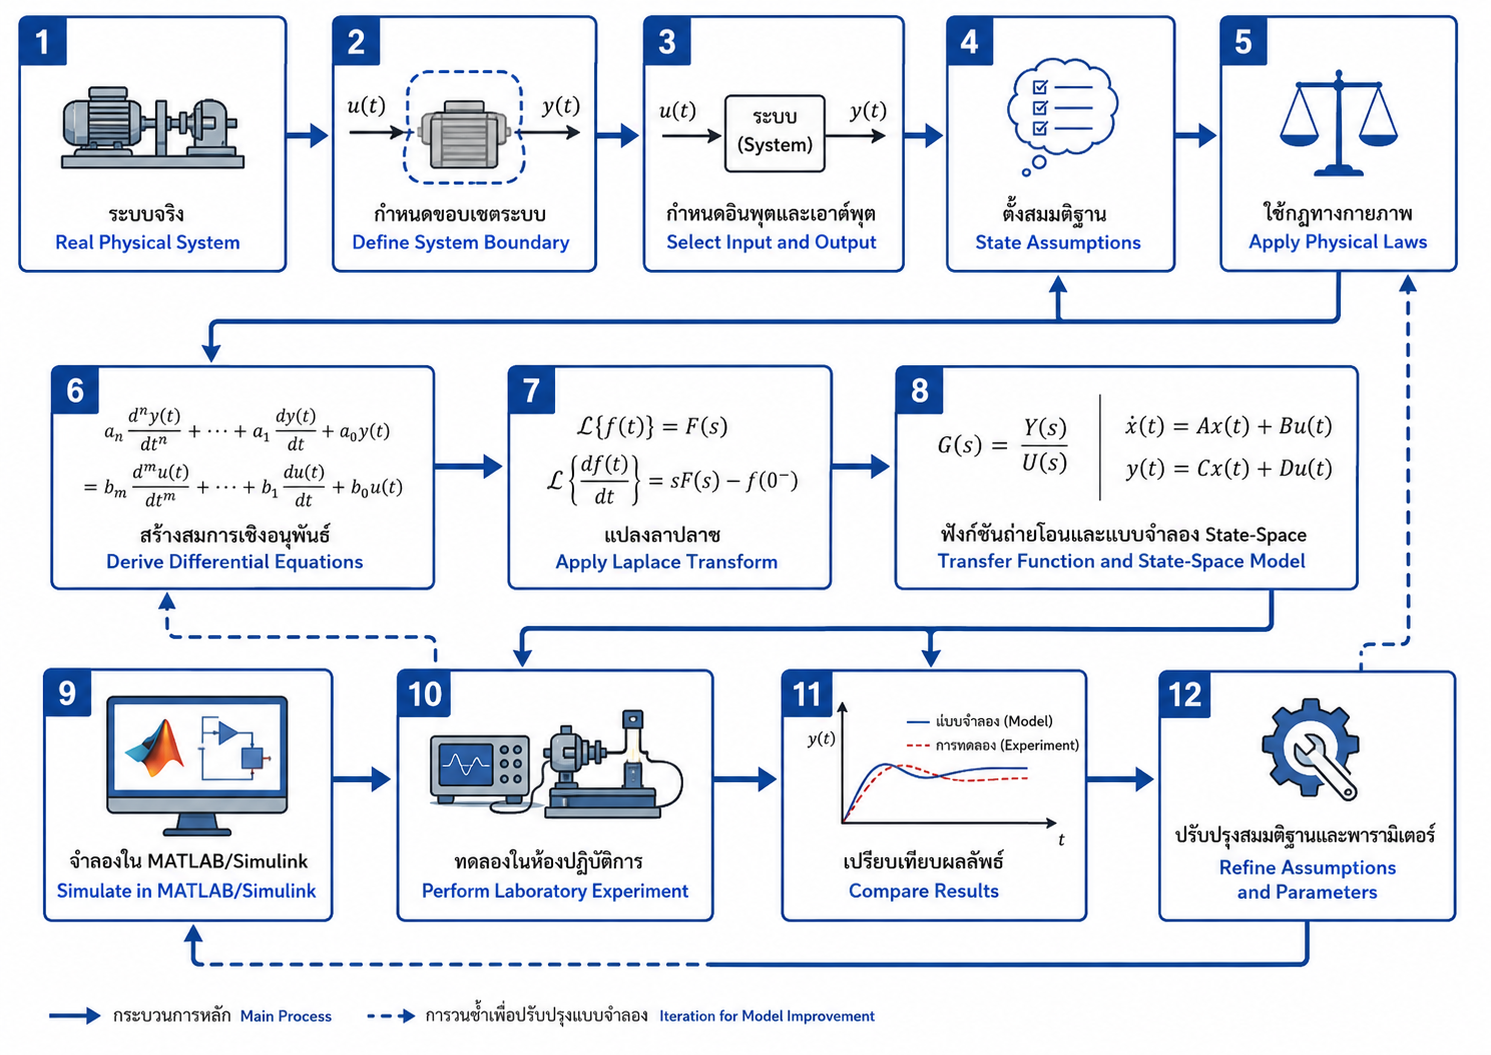
\includegraphics[width=0.8\textwidth]{images/chapter3/figure-1.png}
    \caption{กระบวนการสร้างแบบจำลองระบบควบคุมจากระบบจริงสู่การตรวจสอบแบบจำลอง}
\end{figure}

\par\noindent\rule{\textwidth}{0.4pt}\par

\subsection{6. บทนำ}

การออกแบบระบบควบคุมไม่สามารถเริ่มจากการเลือกตัวควบคุมเพียงอย่างเดียว ผู้วิเคราะห์ต้องทราบก่อนว่าเมื่ออินพุตเปลี่ยน ระบบจริงตอบสนองอย่างไร ตัวอย่างเช่น เมื่อป้อนแรงดันให้มอเตอร์ กระแสจะเพิ่มขึ้นก่อนที่ความเร็วจะเปลี่ยน เมื่อออกแรงต่อระบบมวล–สปริง มวลอาจสั่นและค่อย ๆ หยุดจากผลของแรงหน่วง หรือเมื่อป้อนแรงดันสลับให้วงจร RLC ขนาดและเฟสของแรงดันเอาต์พุตจะเปลี่ยนตามความถี่

การสร้างแบบจำลองจึงเป็นสะพานเชื่อมระหว่างกฎทางฟิสิกส์กับเครื่องมือวิเคราะห์ระบบควบคุม แบบจำลองที่ดีไม่จำเป็นต้องรวมรายละเอียดทุกอย่างของระบบจริง แต่ต้องเก็บลักษณะพลวัตที่สำคัญต่อวัตถุประสงค์ของการศึกษาไว้ ตัวอย่างเช่น หากต้องการศึกษาความเร็วรอบของมอเตอร์ อาจละเลยความยืดหยุ่นของเพลา แต่ต้องคงความเหนี่ยวนำของขดลวด ความต้านทาน โมเมนต์ความเฉื่อย แรงเสียดทาน และแรงเคลื่อนไฟฟ้าย้อนกลับไว้ตามระดับความแม่นยำที่ต้องการ

ความถูกต้องของแบบจำลองจึงขึ้นกับสามองค์ประกอบสำคัญ ได้แก่

\begin{itemize}
    \item การเลือกขอบเขตและตัวแปรที่เหมาะสม
    \item การใช้กฎทางฟิสิกส์และเครื่องหมายอย่างถูกต้อง
    \item การตรวจสอบแบบจำลองกับข้อมูลหรือพฤติกรรมของระบบจริง
\end{itemize}

\par\noindent\rule{\textwidth}{0.4pt}\par

\subsection{7. เนื้อหาหลัก}

\subsubsection{7.1 ความหมายของแบบจำลองทางคณิตศาสตร์ในระบบควบคุม}

\textbf{แบบจำลองทางคณิตศาสตร์} คือ ชุดสมการ ความสัมพันธ์ หรือกฎที่อธิบายพฤติกรรมของระบบด้วยตัวแปรและพารามิเตอร์ แบบจำลองอาจอยู่ในรูปสมการเชิงอนุพันธ์ ฟังก์ชันถ่ายโอน สมการสถานะ แผนภาพบล็อก หรือแบบจำลองเชิงตัวเลข

แบบจำลองในระบบควบคุมมักมุ่งตอบคำถามต่อไปนี้

\begin{enumerate}
    \item อินพุตใดเป็นตัวกระตุ้นระบบ
    \item เอาต์พุตใดเป็นตัวแปรที่ต้องการวัดหรือควบคุม
    \item ระบบสะสมพลังงานหรือข้อมูลไว้ในองค์ประกอบใด
    \item พารามิเตอร์ใดกำหนดความเร็ว การสั่น การหน่วง และอัตราขยายของระบบ
    \item แบบจำลองมีความถูกต้องในช่วงการทำงานใด
\end{enumerate}

\paragraph{7.1.1 แบบจำลองเชิงกายภาพและแบบจำลองเชิงข้อมูล}

\begin{itemize}
    \item \textbf{แบบจำลองเชิงกายภาพ (Physics-Based Model)} สร้างจากกฎทางกล ไฟฟ้า ความร้อน หรือของไหล พารามิเตอร์มักมีความหมายทางกายภาพชัดเจน
    \item \textbf{แบบจำลองเชิงข้อมูล (Data-Driven Model)} สร้างจากข้อมูลอินพุต–เอาต์พุตที่วัดได้ โดยประมาณโครงสร้างและพารามิเตอร์ให้สอดคล้องกับข้อมูล
\end{itemize}

บทนี้เน้นแบบจำลองเชิงกายภาพ เพราะช่วยให้ผู้เรียนเข้าใจว่าพฤติกรรมพลวัตเกิดจากองค์ประกอบใด และสามารถติดตามที่มาของสมการได้

\paragraph{7.1.2 ขั้นตอนทั่วไปในการสร้างแบบจำลอง}

\begin{enumerate}
    \item กำหนดวัตถุประสงค์ของแบบจำลอง
    \item กำหนดขอบเขตของระบบ
    \item เลือกอินพุต เอาต์พุต และตัวแปรภายใน
    \item กำหนดทิศทางบวก จุดอ้างอิง และเครื่องหมาย
    \item ระบุสมมติฐานและเงื่อนไขการทำงาน
    \item ใช้กฎทางฟิสิกส์สร้างสมการ
    \item จัดรูปเป็นสมการเชิงอนุพันธ์
    \item แปลงเป็นฟังก์ชันถ่ายโอนหรือสมการสถานะ
    \item ตรวจสอบหน่วย อันดับ และพฤติกรรมขอบเขต
    \item เปรียบเทียบกับการจำลองหรือผลทดลองและปรับปรุงแบบจำลอง
\end{enumerate}

\paragraph{7.1.3 สมมติฐานที่พบบ่อย}

\begin{itemize}
    \item พารามิเตอร์คงที่ตามเวลา
    \item องค์ประกอบทำงานในช่วงเชิงเส้น
    \item ไม่มีการอิ่มตัว ฮิสเทอรีซิส หรือเดดโซน
    \item ไม่มีความล่าช้าที่ไม่ได้ระบุ
    \item สายไฟและจุดต่อเป็นอุดมคติ
    \item มวล สปริง ตัวหน่วง ตัวต้านทาน ตัวเหนี่ยวนำ และตัวเก็บประจุเป็นองค์ประกอบรวมศูนย์
    \item ผลของสัญญาณรบกวนและความไม่แน่นอนถูกละเลยในแบบจำลองเริ่มต้น
\end{itemize}

แบบจำลองที่มีสมมติฐานมากเกินไปอาจง่ายต่อการวิเคราะห์แต่ไม่สอดคล้องกับระบบจริง ขณะที่แบบจำลองละเอียดเกินไปอาจซับซ้อนโดยไม่เพิ่มประโยชน์ต่อวัตถุประสงค์การควบคุม

\par\noindent\rule{\textwidth}{0.4pt}\par

\subsubsection{7.2 สมการเชิงอนุพันธ์และการแปลงลาปลาซ}

สมการเชิงอนุพันธ์แสดงความสัมพันธ์ระหว่างอินพุต เอาต์พุต และอนุพันธ์ตามเวลา สำหรับระบบเชิงเส้นไม่แปรตามเวลาทั่วไป อาจเขียนได้เป็น

\[
a_n\frac{d^n y(t)}{dt^n}+a_{n-1}\frac{d^{n-1}y(t)}{dt^{n-1}}+\cdots+a_1\frac{dy(t)}{dt}+a_0y(t)
=
b_m\frac{d^m u(t)}{dt^m}+\cdots+b_1\frac{du(t)}{dt}+b_0u(t)
\]

โดยที่

\begin{itemize}
    \item $u(t)$ คืออินพุต
    \item $y(t)$ คือเอาต์พุต
    \item $a_i$ และ $b_i$ คือสัมประสิทธิ์คงที่
    \item $n$ คืออันดับสูงสุดของอนุพันธ์เอาต์พุต
\end{itemize}

เมื่อใช้การแปลงลาปลาซกับอนุพันธ์อันดับหนึ่ง จะได้

\[
\mathcal{L}\left\{\frac{dy(t)}{dt}\right\}=sY(s)-y(0^-)
\]

และสำหรับอนุพันธ์อันดับสอง

\[
\mathcal{L}\left\{\frac{d^2y(t)}{dt^2}\right\}=s^2Y(s)-sy(0^-)-\dot{y}(0^-)
\]

หากกำหนดค่าเริ่มต้นเป็นศูนย์ สมการอนุพันธ์จะเปลี่ยนเป็นสมการพีชคณิตใน $s$ เช่น

\[
a_ns^nY(s)+a_{n-1}s^{n-1}Y(s)+\cdots+a_0Y(s)
=
\left(b_ms^m+\cdots+b_0\right)U(s)
\]

% [รูปที่ 2: การเชื่อมโยงโดเมนเวลาและโดเมน $s$]
% ประเภทภาพ: Infographic / Equation Map
% ตำแหน่งที่แนะนำ: หลังหัวข้อ 7.2
% วัตถุประสงค์การเรียนรู้: แสดงว่าการแปลงลาปลาซเปลี่ยนอนุพันธ์เป็นพหุนามของ $s$ อย่างไร
% คำอธิบายภาพ: ด้านซ้ายเป็นสมการเชิงอนุพันธ์ในเวลา ตรงกลางเป็นลูกศร Laplace Transform พร้อมเงื่อนไข zero initial conditions ด้านขวาเป็นสมการพีชคณิตและอัตราส่วน $G(s)=Y(s)/U(s)$
% องค์ประกอบที่ต้องมี: $y(t)$, $u(t)$, อนุพันธ์, $Y(s)$, $U(s)$, พหุนามของ $s$, เงื่อนไขค่าเริ่มต้นเป็นศูนย์
% ข้อความหรือป้ายกำกับ: Time Domain, Laplace Transform, $s$-Domain, Zero Initial Conditions
% ภาษาของป้ายกำกับ: ไทยและอังกฤษ
% สัดส่วนภาพ: 16:9
% Image Generation Prompt: Educational equation-map infographic connecting a linear differential equation in the time domain to an algebraic equation in the Laplace s-domain. Show input u(t), output y(t), first and second derivatives, a central arrow labeled Laplace Transform with zero initial conditions, and the resulting ratio G(s)=Y(s)/U(s). Clean engineering textbook layout, bilingual Thai-English labels, white background, dark blue equations.
% Alt Text: ภาพแสดงการใช้ลาปลาซเปลี่ยนสมการเชิงอนุพันธ์ในเวลาเป็นฟังก์ชันถ่ายโอนในโดเมนเอส

\begin{figure}[htbp]
    \centering
    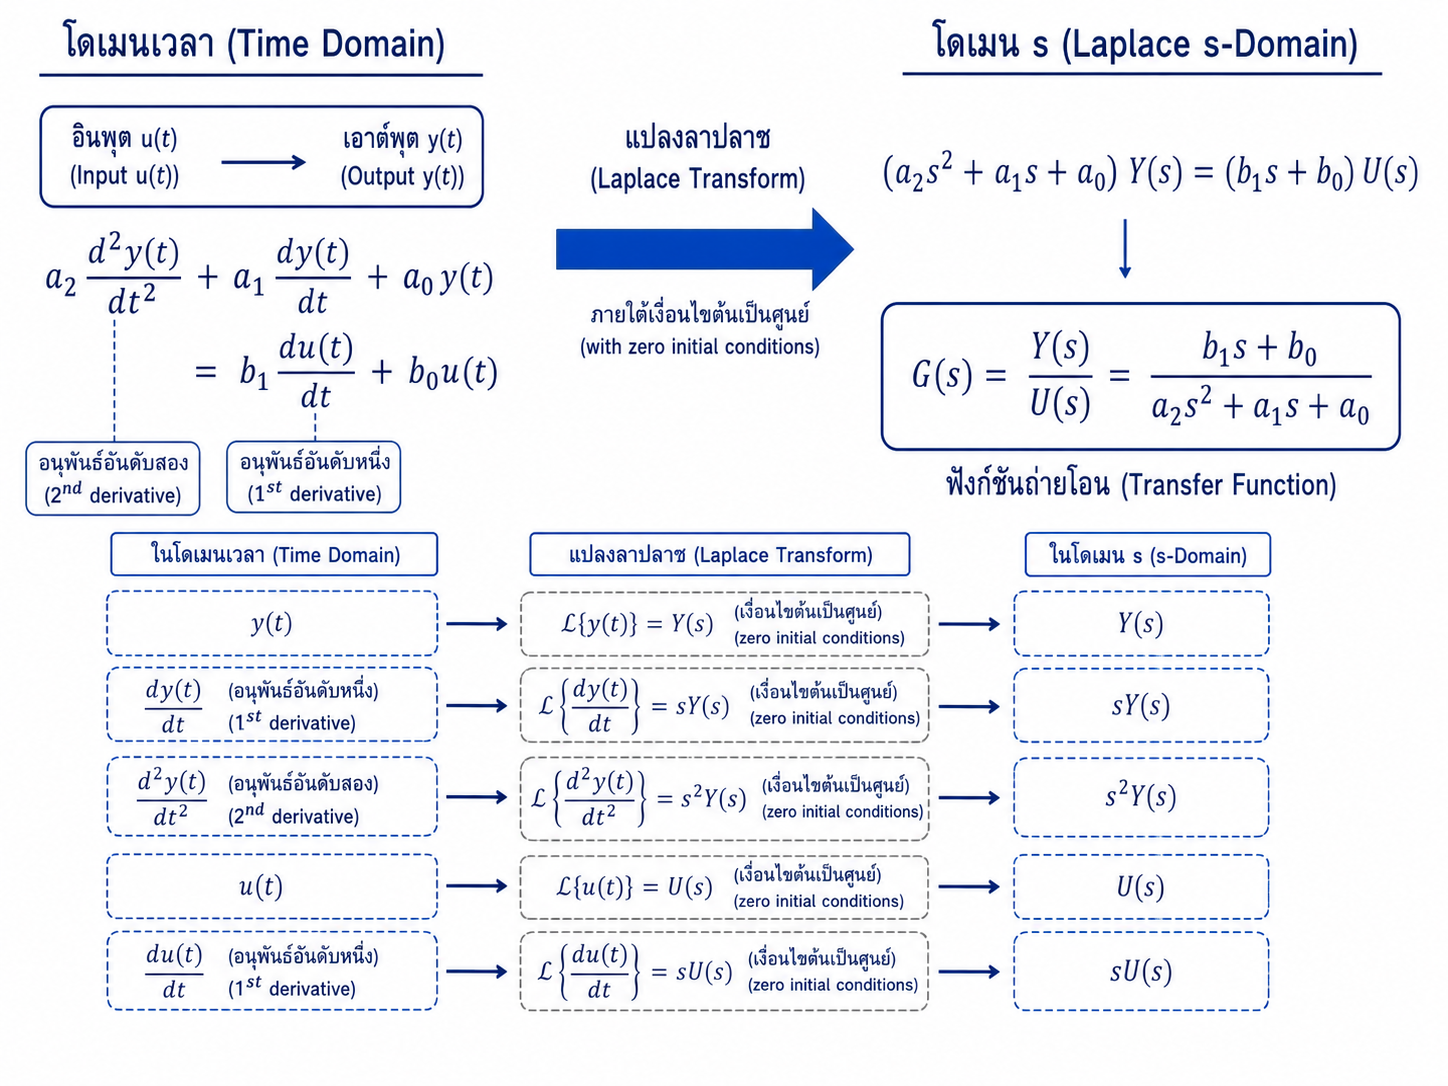
\includegraphics[width=0.8\textwidth]{images/chapter3/figure-2.png}
    \caption{การเชื่อมโยงโดเมนเวลาและโดเมน $s$}
\end{figure}

\par\noindent\rule{\textwidth}{0.4pt}\par

\subsubsection{7.3 นิยามและเงื่อนไขของฟังก์ชันถ่ายโอน}

สำหรับระบบเชิงเส้นไม่แปรตามเวลาที่มีอินพุต $u(t)$ และเอาต์พุต $y(t)$ ฟังก์ชันถ่ายโอนนิยามเป็นอัตราส่วนในโดเมนลาปลาซภายใต้ค่าเริ่มต้นเป็นศูนย์ (MathWorks, n.d.)

\[
G(s)=\frac{Y(s)}{U(s)}\bigg|_{\text{initial conditions}=0}
\]

ฟังก์ชันถ่ายโอนทั่วไปเขียนได้เป็น

\[
G(s)=\frac{b_ms^m+b_{m-1}s^{m-1}+\cdots+b_1s+b_0}
{a_ns^n+a_{n-1}s^{n-1}+\cdots+a_1s+a_0}
\]

\paragraph{7.3.1 ความหมายของตัวแปรและหน่วย}

\begin{itemize}
    \item $s=\sigma+j\omega$ เป็นตัวแปรเชิงซ้อน หน่วยโดยทั่วไปเทียบเท่า $\text{s}^{-1}$
    \item $Y(s)$ และ $U(s)$ เป็นการแปลงลาปลาซของเอาต์พุตและอินพุต
    \item หน่วยของ $G(s)$ ขึ้นกับชนิดของอินพุตและเอาต์พุต เช่น $\text{m/N}$, $\text{rad}\,\text{s}^{-1}\text{/V}$ หรือไม่มีหน่วย
\end{itemize}

\paragraph{7.3.2 เงื่อนไขการใช้ Transfer Function}

\begin{enumerate}
    \item ระบบต้องเป็นเชิงเส้น หรือถูกทำให้เป็นเชิงเส้นรอบจุดทำงาน
    \item พารามิเตอร์ของระบบต้องไม่แปรตามเวลาในช่วงที่พิจารณา
    \item นิยามมาตรฐานใช้ค่าเริ่มต้นเป็นศูนย์
    \item ต้องระบุอินพุตและเอาต์พุตให้ชัดเจน เพราะระบบเดียวกันอาจมีฟังก์ชันถ่ายโอนต่างกันเมื่อเปลี่ยนเอาต์พุต
    \item สำหรับการใช้งานพื้นฐานในบทนี้ เน้นระบบอินพุตเดียวเอาต์พุตเดียว
    \item พหุนามส่วนต้องไม่เป็นศูนย์ทุกสัมประสิทธิ์ และควรจัดเรียงตามกำลังของ $s$
    \item ในแบบจำลองที่นำไปใช้กับบล็อก Transfer Fcn โดยตรง โดยทั่วไปอันดับส่วนต้องไม่น้อยกว่าอันดับเศษ
\end{enumerate}

\paragraph{7.3.3 ความหมายทางกายภาพ}

ฟังก์ชันถ่ายโอนไม่ได้หมายถึงการหารสัญญาณในโดเมนเวลา แต่เป็นตัวดำเนินการเชิงพลวัตที่บอกว่าองค์ประกอบของสัญญาณอินพุตถูกขยาย ลดทอน หน่วงเฟส หรือเปลี่ยนรูปอย่างไร เมื่อใช้ร่วมกับอินพุตในโดเมน $s$ จะได้

\[
Y(s)=G(s)U(s)
\]

\paragraph{7.3.4 โพล ซีโร และอันดับของระบบ}

\begin{itemize}
    \item \textbf{ซีโร (Zeros)} คือค่าของ $s$ ที่ทำให้พหุนามเศษเป็นศูนย์
    \item \textbf{โพล (Poles)} คือค่าของ $s$ ที่ทำให้พหุนามส่วนเป็นศูนย์
    \item \textbf{อันดับของระบบ} โดยทั่วไปสัมพันธ์กับกำลังสูงสุดของพหุนามส่วนหลังตัดตัวประกอบร่วมแล้ว
\end{itemize}

โพลสัมพันธ์อย่างใกล้ชิดกับรูปแบบการตอบสนองตามเวลา ส่วนซีโรมีผลต่อรูปร่าง ขนาด และเฟสของการตอบสนอง อย่างไรก็ตาม การวิเคราะห์เสถียรภาพและการตอบสนองเชิงลึกจะศึกษาในบทถัดไป

\paragraph{7.3.5 ข้อจำกัด}

\begin{itemize}
    \item ไม่แสดงสภาวะภายในทั้งหมดของระบบ
    \item ไม่รวมผลจากค่าเริ่มต้นที่ไม่เป็นศูนย์ไว้ในนิยาม
    \item แบบจำลองเชิงเส้นอาจไม่ถูกต้องเมื่อระบบอิ่มตัวหรือทำงานไกลจากจุดทำงาน
    \item ระบบที่มีพารามิเตอร์เปลี่ยนตามเวลาและระบบไม่เชิงเส้นต้องใช้วิธีอื่นหรือสร้างแบบจำลองประมาณ
    \item การแทนระบบหลายอินพุตหลายเอาต์พุตต้องใช้เมทริกซ์ของฟังก์ชันถ่ายโอนหรือสมการสถานะ
\end{itemize}

\paragraph{7.3.6 ตัวอย่างพื้นฐาน: จากสมการเชิงอนุพันธ์เป็น Transfer Function}

\textbf{ตัวอย่างเพิ่มเติมเพื่อการเรียนรู้}\\กำหนดระบบ

\[
2\ddot{y}(t)+5\dot{y}(t)+3y(t)=4u(t)
\]

\textbf{ขั้นที่ 1 วิเคราะห์ระบบ}\\อินพุตคือ $u(t)$ และเอาต์พุตคือ $y(t)$ ระบบเป็นสมการเชิงเส้นอันดับสอง

\textbf{ขั้นที่ 2 กำหนดเงื่อนไข}\\ใช้ค่าเริ่มต้นเป็นศูนย์ คือ $y(0^-)=0$ และ $\dot{y}(0^-)=0$

\textbf{ขั้นที่ 3 แปลงลาปลาซ}

\[
2s^2Y(s)+5sY(s)+3Y(s)=4U(s)
\]

\textbf{ขั้นที่ 4 จัดรูป}

\[
\left(2s^2+5s+3\right)Y(s)=4U(s)
\]

ดังนั้น

\[
G(s)=\frac{Y(s)}{U(s)}=\frac{4}{2s^2+5s+3}
\]

\textbf{ตรวจสอบ}\\อันดับของระบบเท่ากับ 2 และหน่วยของฟังก์ชันถ่ายโอนขึ้นกับหน่วยของ $y$ และ $u$

\par\noindent\rule{\textwidth}{0.4pt}\par

\subsubsection{7.4 การสร้างแบบจำลองระบบทางกล}

ระบบทางกลเชิงเส้นที่พบบ่อยประกอบด้วยมวล สปริง และตัวหน่วงหนืด

\begin{table}[htbp]
    \centering
    \begin{tabular}{l l l l}
        \hline
        \textbf{องค์ประกอบ} & \textbf{ความสัมพันธ์ในโดเมนเวลา} & \textbf{พารามิเตอร์และหน่วย} & \textbf{ความหมาย} \\
        \hline
        มวล & $F_m(t)=m\ddot{x}(t)$ & $m$ หน่วย kg & ต้านการเปลี่ยนแปลงความเร็ว \\
        สปริง & $F_k(t)=kx(t)$ & $k$ หน่วย N/m & สะสมพลังงานศักย์และสร้างแรงคืนตัว \\
        ตัวหน่วง & $F_c(t)=c\dot{x}(t)$ & $c$ หน่วย N·s/m & สลายพลังงานและลดการสั่น \\
        \hline
    \end{tabular}
\end{table}

\paragraph{7.4.1 การกำหนดทิศทางและ Free-Body Diagram}

ก่อนเขียนสมการ ต้องกำหนดทิศทางบวกของการกระจัด $x(t)$ และวาดแรงทั้งหมดบนมวล หากกำหนดทิศทางบวกไปทางขวา แรงสปริงและแรงหน่วงที่ต้านการเคลื่อนที่จะมีเครื่องหมายตรงข้ามกับ $x(t)$ และ $\dot{x}(t)$ ตามลำดับ

% [รูปที่ 3: ระบบมวล–สปริง–ตัวหน่วงและแผนภาพแรง]
% ประเภทภาพ: Technical Illustration
% ตำแหน่งที่แนะนำ: ก่อนสมการระบบมวล–สปริง–ตัวหน่วง
% วัตถุประสงค์การเรียนรู้: ช่วยกำหนดแรง ทิศทาง และเครื่องหมายก่อนสร้างสมการ
% คำอธิบายภาพ: แสดงมวล $m$ บนพื้นราบ เชื่อมกับผนังด้วยสปริง $k$ และตัวหน่วง $c$ แบบขนาน มีแรงอินพุต $F(t)$ ไปทางขวา การกระจัด $x(t)$ ไปทางขวา และภาพย่อย Free-Body Diagram ของมวลพร้อมแรง $F(t)$, $kx(t)$ และ $c\dot{x}(t)$
% องค์ประกอบที่ต้องมี: ผนัง มวล สปริง ตัวหน่วง ลูกศรแรง ลูกศรการกระจัด และแกนอ้างอิง
% ข้อความหรือป้ายกำกับ: $m$, $k$, $c$, $F(t)$, $x(t)$, $kx(t)$, $c\dot{x}(t)$
% ภาษาของป้ายกำกับ: สัญลักษณ์สากลและอังกฤษ
% สัดส่วนภาพ: 16:9
% Image Generation Prompt: Mechanical engineering textbook diagram of a translational mass-spring-damper system. A mass m rests on a horizontal frictionless surface and is connected to a fixed wall by a spring k and viscous damper c in parallel. An external force F(t) acts to the right and displacement x(t) is positive to the right. Include a separate free-body diagram of the mass showing F(t) to the right and restoring forces kx(t) and c x-dot(t) to the left. Clean black line art, white background, accurate technical symbols.
% Alt Text: ระบบมวลต่อกับสปริงและตัวหน่วง พร้อมแผนภาพแรงที่ใช้สร้างสมการการเคลื่อนที่

\begin{figure}[htbp]
    \centering
    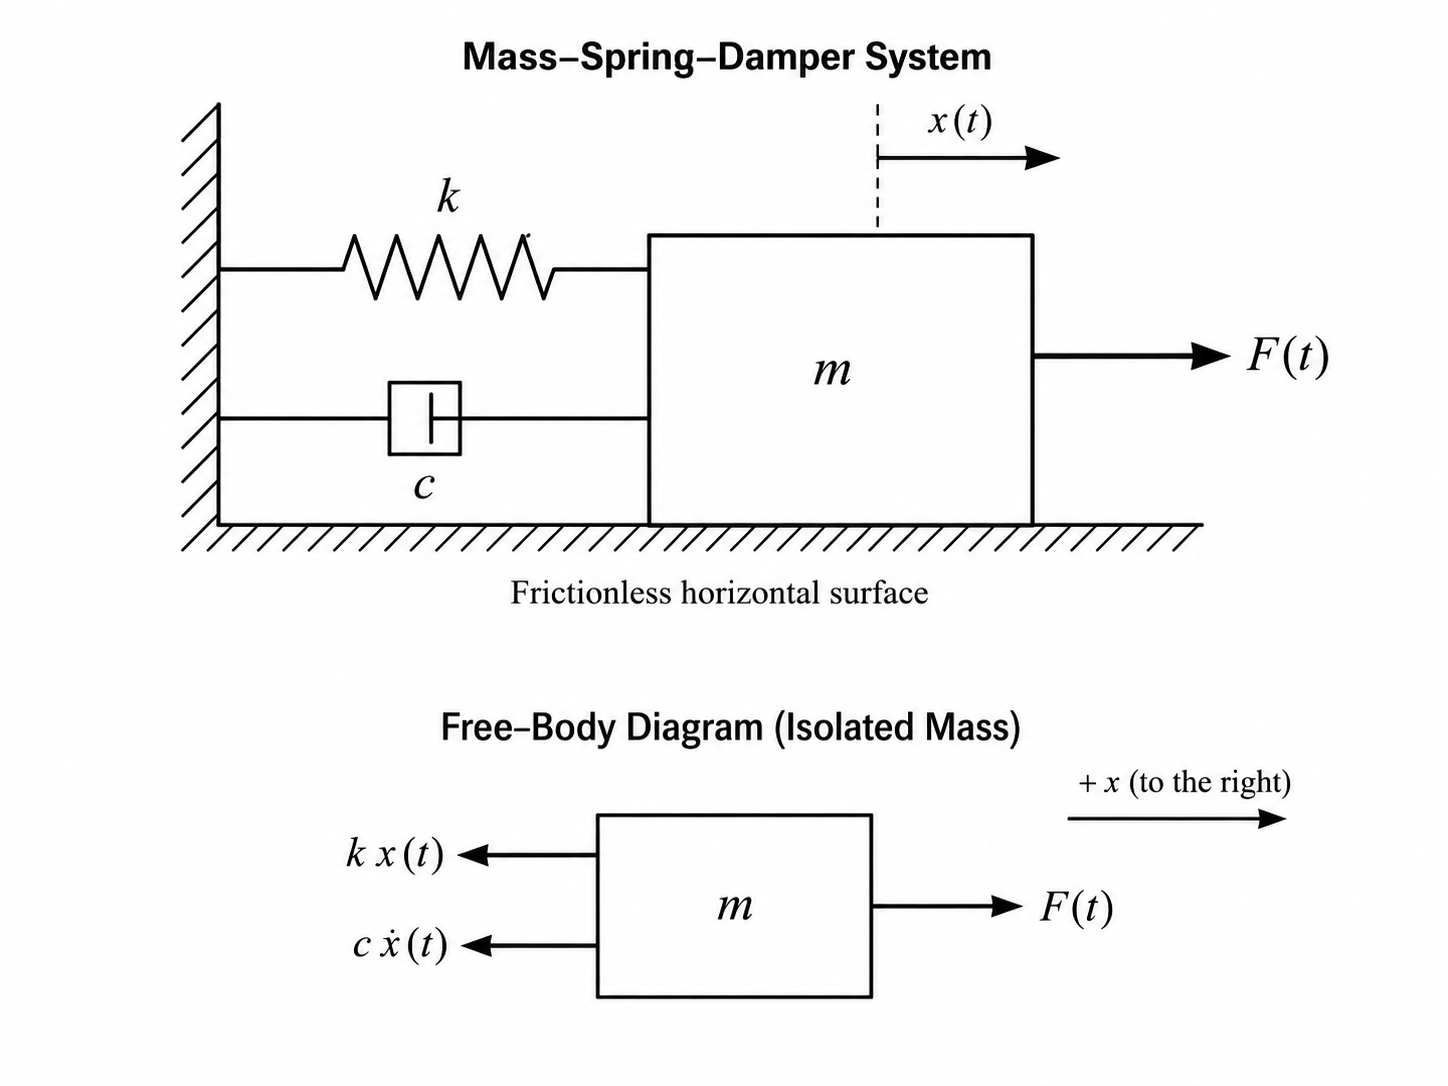
\includegraphics[width=0.8\textwidth]{images/chapter3/figure-3.png}
    \caption{ระบบมวล–สปริง–ตัวหน่วงและแผนภาพแรง}
\end{figure}

\paragraph{7.4.2 สมการของระบบมวล–สปริง–ตัวหน่วง}

ใช้กฎข้อที่สองของนิวตัน

\[
\sum F(t)=m\ddot{x}(t)
\]

เมื่อรวมแรงในทิศบวก จะได้

\[
F(t)-c\dot{x}(t)-kx(t)=m\ddot{x}(t)
\]

จัดรูปเป็น

\[
m\ddot{x}(t)+c\dot{x}(t)+kx(t)=F(t)
\]

ภายใต้ค่าเริ่มต้นเป็นศูนย์

\[
\left(ms^2+cs+k\right)X(s)=F(s)
\]

ดังนั้น ฟังก์ชันถ่ายโอนจากแรงไปยังการกระจัดคือ

\[
G_x(s)=\frac{X(s)}{F(s)}=\frac{1}{ms^2+cs+k}
\]

หากเลือกความเร็ว $v(t)=\dot{x}(t)$ เป็นเอาต์พุต จะได้

\[
G_v(s)=\frac{V(s)}{F(s)}=\frac{s}{ms^2+cs+k}
\]

สมการทั้งสองอธิบายระบบทางกายภาพเดียวกัน แต่แตกต่างกันเพราะเลือกเอาต์พุตต่างกัน

\paragraph{7.4.3 พารามิเตอร์มาตรฐานของระบบอันดับสอง}

หารสมการส่วนด้วย $m$

\[
G_x(s)=\frac{1/m}{s^2+\frac{c}{m}s+\frac{k}{m}}
\]

เปรียบเทียบกับรูปมาตรฐาน

\[
s^2+2\zeta\omega_n s+\omega_n^2
\]

จะได้

\[
\omega_n=\sqrt{\frac{k}{m}}
\]

และ

\[
\zeta=\frac{c}{2\sqrt{mk}}
\]

โดย $\omega_n$ คือความถี่ธรรมชาติไม่หน่วง หน่วย rad/s และ $\zeta$ คืออัตราส่วนการหน่วงซึ่งไม่มีหน่วย

\paragraph{7.4.4 ตัวอย่างบังคับ: ระบบมวล–สปริง–ตัวหน่วง}

\textbf{ตัวอย่างเพิ่มเติมเพื่อการเรียนรู้}\\กำหนด $m=2\ \text{kg}$, $c=6\ \text{N·s/m}$, $k=8\ \text{N/m}$ อินพุตเป็นแรง $F(t)$ และเอาต์พุตเป็นการกระจัด $x(t)$

\textbf{1. วิเคราะห์ระบบ}\\ระบบมีองค์ประกอบสะสมพลังงานสองชนิด คือมวลและสปริง จึงคาดว่าเป็นระบบอันดับสอง

\textbf{2. กำหนดทิศทาง}\\กำหนด $x(t)$ และ $F(t)$ เป็นบวกไปทางขวา

\textbf{3. ใช้กฎของนิวตัน}

\[
2\ddot{x}(t)+6\dot{x}(t)+8x(t)=F(t)
\]

\textbf{4. แปลงลาปลาซภายใต้ค่าเริ่มต้นเป็นศูนย์}

\[
\left(2s^2+6s+8\right)X(s)=F(s)
\]

\textbf{5. ฟังก์ชันถ่ายโอน}

\[
\boxed{\frac{X(s)}{F(s)}=\frac{1}{2s^2+6s+8}}
\]

\textbf{6. ความถี่ธรรมชาติและอัตราส่วนการหน่วง}

\[
\omega_n=\sqrt{\frac{8}{2}}=2\ \text{rad/s}
\]

\[
\zeta=\frac{6}{2\sqrt{(2)(8)}}=0.75
\]

\textbf{7. ตรวจสอบหน่วยและความสมเหตุสมผล}\\เมื่อ $s=0$ อัตราขยายสภาวะคงตัวคือ $1/k=1/8\ \text{m/N}$ ดังนั้นหากป้อนแรงคงที่ $10\ \text{N}$ การกระจัดสภาวะคงตัวตามแบบจำลองคือ

\[
x_{ss}=\frac{10}{8}=1.25\ \text{m}
\]

ค่าดังกล่าวมีขนาดค่อนข้างมาก จึงชี้ให้เห็นว่าสปริงตัวอย่างมีค่าความแข็งต่ำ หากเป็นระบบจริงอาจต้องตรวจสอบว่าการยืดอยู่ในช่วงเชิงเส้นของสปริงหรือไม่

\paragraph{7.4.5 ระบบเชิงหมุนโดยสังเขป}

ระบบเชิงหมุนใช้ความสัมพันธ์ที่คล้ายกัน

\begin{table}[htbp]
    \centering
    \begin{tabular}{l l}
        \hline
        \textbf{การเลื่อนที่} & \textbf{การหมุน} \\
        \hline
        แรง $F$ & แรงบิด $T$ \\
        มวล $m$ & โมเมนต์ความเฉื่อย $J$ \\
        การกระจัด $x$ & มุม $\theta$ \\
        ความเร็ว $\dot{x}$ & ความเร็วเชิงมุม $\omega=\dot{\theta}$ \\
        สัมประสิทธิ์หน่วง $c$ & สัมประสิทธิ์เสียดทานหนืด $b$ \\
        \hline
    \end{tabular}
\end{table}

สมการพื้นฐานคือ

\[
J\ddot{\theta}(t)+b\dot{\theta}(t)+k_\theta\theta(t)=T(t)
\]

\subsubsection{7.5 การสร้างแบบจำลองระบบทางไฟฟ้า}

การสร้างแบบจำลองระบบทางไฟฟ้าเริ่มจากการเลือกแรงดันหรือกระแสที่เป็นอินพุตและเอาต์พุต กำหนดขั้วแรงดันและทิศทางกระแส แล้วใช้กฎแรงดันของเคอร์ชอฟฟ์ (Kirchhoff’s Voltage Law: KVL) หรือกฎกระแสของเคอร์ชอฟฟ์ (Kirchhoff’s Current Law: KCL) ร่วมกับความสัมพันธ์ของอุปกรณ์

\begin{table}[htbp]
    \centering
    \begin{tabular}{l l l l}
        \hline
        \textbf{อุปกรณ์} & \textbf{ความสัมพันธ์ในโดเมนเวลา} & \textbf{อิมพีแดนซ์ในโดเมน $s$ ภายใต้ค่าเริ่มต้นเป็นศูนย์} & \textbf{หน่วยพารามิเตอร์} \\
        \hline
        ตัวต้านทาน $R$ & $v_R(t)=Ri_R(t)$ & $Z_R(s)=R$ & $\Omega$ \\
        ตัวเหนี่ยวนำ $L$ & $v_L(t)=L\dfrac{di_L(t)}{dt}$ & $Z_L(s)=sL$ & H \\
        ตัวเก็บประจุ $C$ & $i_C(t)=C\dfrac{dv_C(t)}{dt}$ & $Z_C(s)=\dfrac{1}{sC}$ & F \\
        \hline
    \end{tabular}
\end{table}

\begin{quote}
\textbf{ข้อควรระวัง:} การใช้ $Z_L=sL$ และ $Z_C=1/(sC)$ ในรูปอย่างง่ายนี้ตั้งอยู่บนสมมติฐานค่าเริ่มต้นเป็นศูนย์ หากตัวเหนี่ยวนำมีกระแสเริ่มต้นหรือตัวเก็บประจุมีแรงดันเริ่มต้น ต้องเพิ่มพจน์ที่เกิดจากพลังงานเริ่มต้นในสมการลาปลาซ
\end{quote}

\paragraph{7.5.1 วงจร RC อนุกรม: เอาต์พุตคร่อมตัวเก็บประจุ}

พิจารณาวงจรที่มีตัวต้านทาน $R$ ต่ออนุกรมกับตัวเก็บประจุ $C$ อินพุตคือ $v_i(t)$ และเอาต์พุตคือแรงดันคร่อมตัวเก็บประจุ $v_o(t)=v_C(t)$

จาก KVL

\[
v_i(t)=v_R(t)+v_C(t)
\]

กระแสในวงจรเท่ากันทุกองค์ประกอบ และ

\[
i(t)=C\frac{dv_o(t)}{dt}
\]

จึงได้

\[
RC\frac{dv_o(t)}{dt}+v_o(t)=v_i(t)
\]

แปลงลาปลาซภายใต้ค่าเริ่มต้นเป็นศูนย์

\[
(RCs+1)V_o(s)=V_i(s)
\]

ดังนั้น

\[
\boxed{G_{RC}(s)=\frac{V_o(s)}{V_i(s)}=\frac{1}{RCs+1}}
\]

นี่คือระบบอันดับหนึ่งที่มีค่าคงตัวเวลา

\[
\tau=RC
\]

และความถี่ตัดเชิงมุม

\[
\omega_c=\frac{1}{RC}
\]

ที่ความถี่ $\omega_c$ ขนาดอัตราขยายของวงจรอุดมคติเท่ากับ $1/\sqrt{2}$ ของค่าที่ความถี่ต่ำ หรือประมาณ $-3\ \text{dB}$

% [รูปที่ 4: การสร้างแบบจำลองวงจร RC และ RL]
% ประเภทภาพ: Technical Illustration / Circuit Diagram
% ตำแหน่งที่แนะนำ: หัวข้อ 7.5.1–7.5.2
% วัตถุประสงค์การเรียนรู้: ช่วยให้ผู้เรียนระบุอินพุต เอาต์พุต ทิศทางกระแส และตำแหน่งวัดแรงดันก่อนสร้างสมการ
% คำอธิบายภาพ: แบ่งภาพเป็นสองส่วน ด้านซ้ายเป็นวงจร RC อนุกรม โดยวัดเอาต์พุตคร่อมตัวเก็บประจุ ด้านขวาเป็นวงจร RL อนุกรม โดยวัดเอาต์พุตคร่อมตัวต้านทาน แสดงลูกศรกระแสและขั้วแรงดันอย่างชัดเจน
% องค์ประกอบที่ต้องมี: แหล่งสัญญาณ $v_i(t)$, ตัวต้านทาน $R$, ตัวเก็บประจุ $C$, ตัวเหนี่ยวนำ $L$, จุดกราวด์, ลูกศรกระแส $i(t)$, เอาต์พุต $v_o(t)$
% ข้อความหรือป้ายกำกับ: “RC Low-Pass”, “RL Low-Pass”, “Input”, “Output”, $R$, $L$, $C$, $i(t)$
% ภาษาของป้ายกำกับ: อังกฤษ
% สัดส่วนภาพ: 16:9
% Image Generation Prompt: Clean educational electrical engineering diagram with two side-by-side circuits. Left: series RC low-pass circuit driven by voltage source vi(t), resistor R followed by capacitor C to ground, output vo(t) measured across C, current arrow i(t). Right: series RL low-pass circuit driven by vi(t), inductor L followed by resistor R to ground, output vo(t) measured across R, current arrow i(t). Use standard IEC/ANSI circuit symbols, clear polarity marks, white background, textbook line-art style, no decorative elements.
% Alt Text: วงจร RC และ RL อนุกรมที่แสดงตำแหน่งอินพุต เอาต์พุต และทิศทางกระแสสำหรับใช้สร้างสมการ

\begin{figure}[htbp]
    \centering
    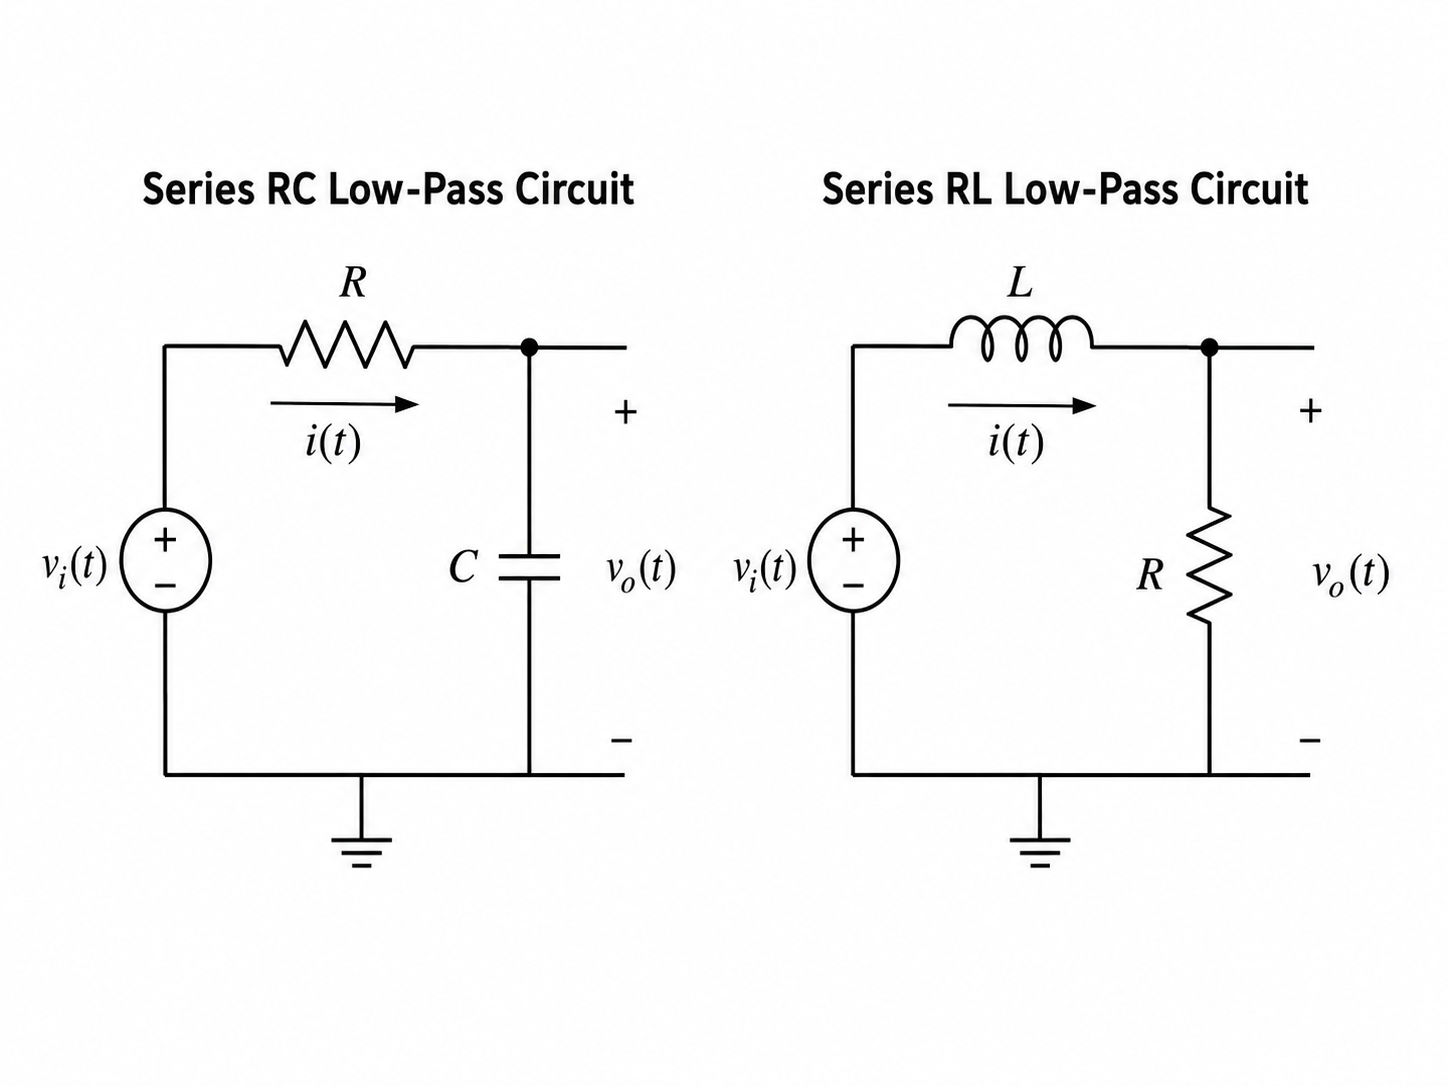
\includegraphics[width=0.8\textwidth]{images/chapter3/figure-4.png}
    \caption{การสร้างแบบจำลองวงจร RC และ RL}
\end{figure}

\paragraph{7.5.2 วงจร RL อนุกรม: เอาต์พุตคร่อมตัวต้านทาน}

จาก KVL

\[
v_i(t)=L\frac{di(t)}{dt}+Ri(t)
\]

เมื่อ $v_o(t)=Ri(t)$ จะได้ $i(t)=v_o(t)/R$ ดังนั้น

\[
\frac{L}{R}\frac{dv_o(t)}{dt}+v_o(t)=v_i(t)
\]

ฟังก์ชันถ่ายโอนคือ

\[
\boxed{G_{RL,R}(s)=\frac{V_o(s)}{V_i(s)}=\frac{R}{Ls+R}
=\frac{1}{\left(\frac{L}{R}\right)s+1}}
\]

ค่าคงตัวเวลาคือ

\[
\tau=\frac{L}{R}
\]

หากเลือกเอาต์พุตคร่อมตัวเหนี่ยวนำแทน จะได้

\[
\boxed{G_{RL,L}(s)=\frac{Ls}{Ls+R}}
\]

ตัวอย่างนี้ย้ำว่า \textbf{วงจรเดียวกันอาจมีฟังก์ชันถ่ายโอนต่างกันตามตำแหน่งเอาต์พุต} วงจรที่วัดคร่อม $R$ มีลักษณะผ่านต่ำ ส่วนวงจรที่วัดคร่อม $L$ มีลักษณะผ่านสูง

\paragraph{7.5.3 วงจร RLC อนุกรม: เอาต์พุตคร่อมตัวเก็บประจุ}

พิจารณาวงจร RLC อนุกรม อินพุตคือ $v_i(t)$ และเอาต์พุตคือ $v_o(t)=v_C(t)$

จาก KVL

\[
v_i(t)=v_R(t)+v_L(t)+v_C(t)
\]

เนื่องจาก

\[
i(t)=C\frac{dv_o(t)}{dt}
\]

จึงมี

\[
v_R(t)=RC\frac{dv_o(t)}{dt}
\]

และ

\[
v_L(t)=LC\frac{d^2v_o(t)}{dt^2}
\]

ดังนั้น

\[
LC\frac{d^2v_o(t)}{dt^2}
+RC\frac{dv_o(t)}{dt}
+v_o(t)=v_i(t)
\]

เมื่อค่าเริ่มต้นเป็นศูนย์

\[
\left(LCs^2+RCs+1\right)V_o(s)=V_i(s)
\]

จึงได้

\[
\boxed{G_{RLC}(s)=\frac{V_o(s)}{V_i(s)}
=\frac{1}{LCs^2+RCs+1}}
\]

หารส่วนด้วย $LC$

\[
G_{RLC}(s)=\frac{1/(LC)}
{s^2+\frac{R}{L}s+\frac{1}{LC}}
\]

เปรียบเทียบกับรูปมาตรฐานอันดับสอง จะได้

\[
\omega_n=\frac{1}{\sqrt{LC}}
\]

\[
\zeta=\frac{R}{2}\sqrt{\frac{C}{L}}
\]

ในวงจรจริงควรแทน $R$ ด้วยความต้านทานอนุกรมรวม

\[
R_{\text{eq}}=R+R_s+r_L+r_{\text{wire}}
\]

เมื่อ $R_s$ คือความต้านทานเอาต์พุตของเครื่องกำเนิดสัญญาณ และ $r_L$ คือความต้านทานขดลวดของตัวเหนี่ยวนำ แบบจำลองที่ละเลยค่าดังกล่าวมักทำนายยอดเรโซแนนซ์สูงกว่าผลทดลอง

% [รูปที่ 5: วงจร RLC อุดมคติและแบบจำลองเชิงปฏิบัติ]
% ประเภทภาพ: Circuit Diagram / Comparative Technical Illustration
% ตำแหน่งที่แนะนำ: หัวข้อ 7.5.3
% วัตถุประสงค์การเรียนรู้: แสดงความแตกต่างระหว่างแบบจำลองอุดมคติกับแบบจำลองที่รวมพารามิเตอร์แฝง
% คำอธิบายภาพ: แสดงวงจร RLC อนุกรมสองวงจรแบบเคียงข้างกัน วงจรแรกใช้ $R$, $L$, $C$ อุดมคติ วงจรที่สองเพิ่ม $R_s$ ของแหล่งกำเนิดและ $r_L$ อนุกรมกับตัวเหนี่ยวนำ พร้อมวัดเอาต์พุตคร่อมตัวเก็บประจุ
% องค์ประกอบที่ต้องมี: แหล่งสัญญาณ, $R_s$, $R$, $r_L$, $L$, $C$, จุดกราวด์, $v_i$, $v_o$, ลูกศรกระแส
% ข้อความหรือป้ายกำกับ: “Ideal Model”, “Practical Model”, “Source Resistance”, “Inductor Winding Resistance”
% ภาษาของป้ายกำกับ: อังกฤษ
% สัดส่วนภาพ: 16:9
% Image Generation Prompt: Engineering textbook comparison of two series RLC low-pass circuits. Left panel labeled Ideal Model: source vi, resistor R, ideal inductor L, capacitor C to ground, output vo across C. Right panel labeled Practical Model: include source resistance Rs and inductor winding resistance rL in series in addition to R, L, C; output vo across C. Show current direction and voltage polarity. Use accurate circuit symbols, clean monochrome line art, white background.
% Alt Text: เปรียบเทียบวงจร RLC อุดมคติกับวงจรที่รวมความต้านทานแหล่งกำเนิดและความต้านทานขดลวด

\begin{figure}[htbp]
    \centering
    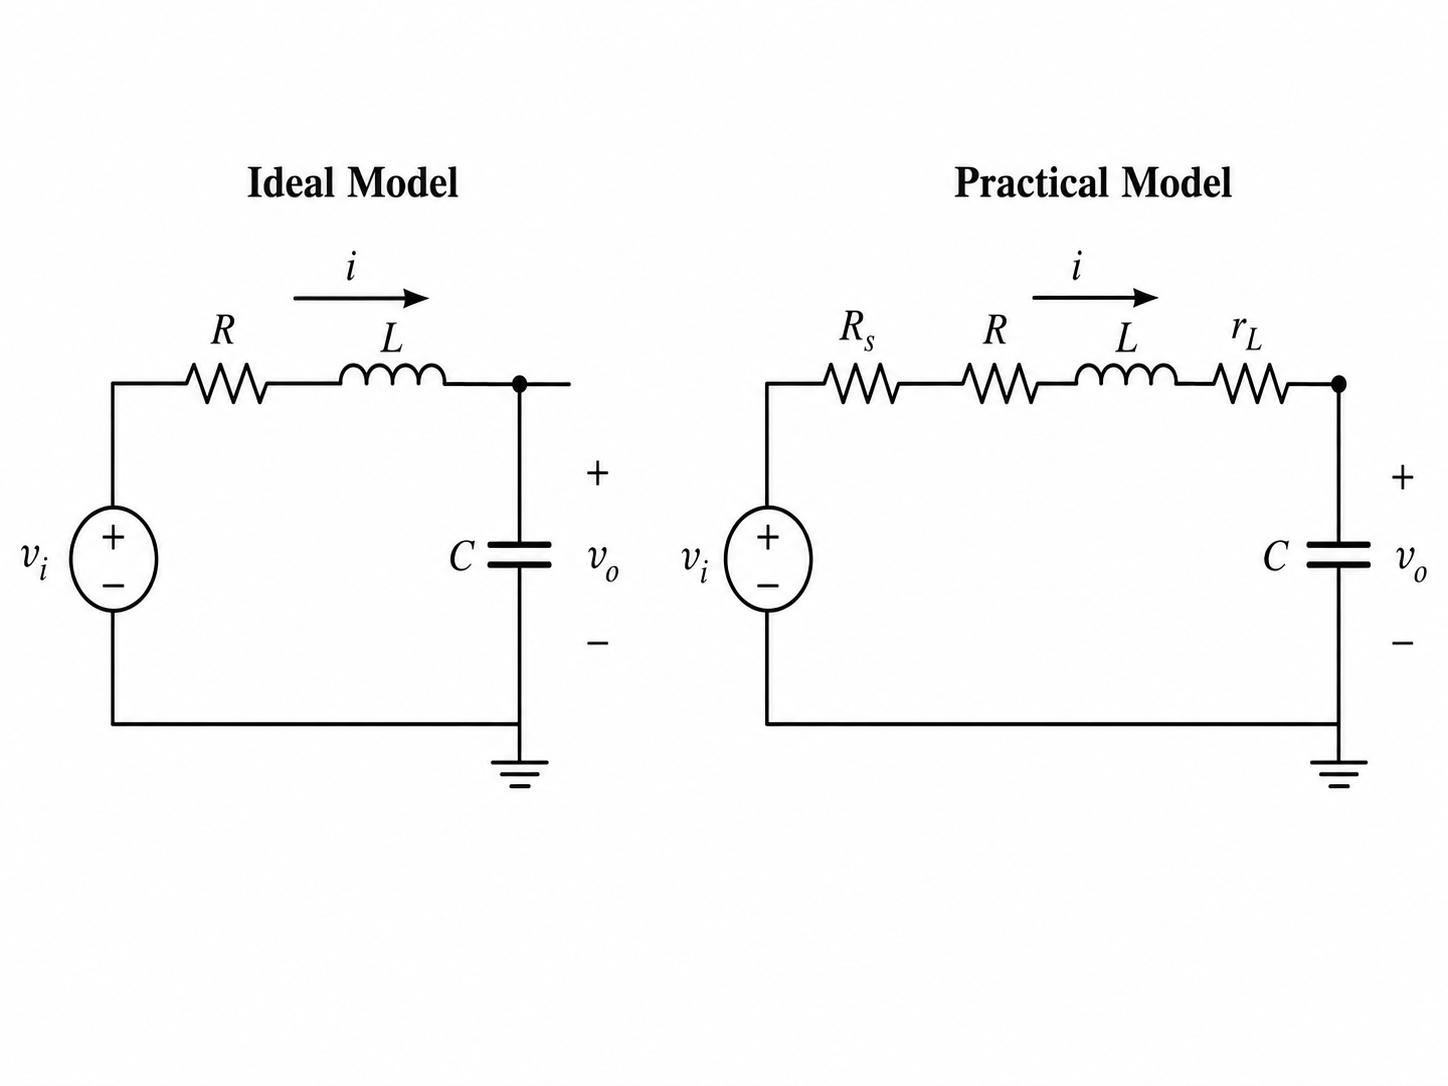
\includegraphics[width=0.8\textwidth]{images/chapter3/figure-5.png}
    \caption{วงจร RLC อุดมคติและแบบจำลองเชิงปฏิบัติ}
\end{figure}

\paragraph{7.5.4 ตัวอย่างบังคับ: หาฟังก์ชันถ่ายโอนของวงจร RLC}

\textbf{ตัวอย่างเพิ่มเติมเพื่อการเรียนรู้}\\กำหนด $R=100\ \Omega$, $L=10\ \text{mH}$ และ $C=1\ \mu\text{F}$ ต่ออนุกรม วัดเอาต์พุตคร่อมตัวเก็บประจุ

\textbf{1. วิเคราะห์ระบบ}\\ตัวเหนี่ยวนำและตัวเก็บประจุเป็นองค์ประกอบสะสมพลังงานสองตัว ระบบจึงเป็นอันดับสอง

\textbf{2. สร้างสมการ}

\[
LC\frac{d^2v_o}{dt^2}+RC\frac{dv_o}{dt}+v_o=v_i
\]

\textbf{3. แทนค่าพารามิเตอร์}

\[
LC=(10\times10^{-3})(1\times10^{-6})=1\times10^{-8}
\]

\[
RC=(100)(1\times10^{-6})=1\times10^{-4}
\]

จึงได้

\[
10^{-8}\frac{d^2v_o}{dt^2}
+10^{-4}\frac{dv_o}{dt}+v_o=v_i
\]

\textbf{4. แปลงเป็นฟังก์ชันถ่ายโอน}

\[
\boxed{
G(s)=\frac{V_o(s)}{V_i(s)}
=\frac{1}{10^{-8}s^2+10^{-4}s+1}
}
\]

หรือคูณทั้งเศษและส่วนด้วย $10^8$

\[
\boxed{
G(s)=\frac{10^8}{s^2+10^4s+10^8}
}
\]

\textbf{5. คำนวณพารามิเตอร์อันดับสอง}

\[
\omega_n=\frac{1}{\sqrt{LC}}
=\frac{1}{\sqrt{10^{-8}}}
=10{,}000\ \text{rad/s}
\]

\[
f_n=\frac{\omega_n}{2\pi}
\approx1{,}591.55\ \text{Hz}
\]

\[
\zeta=\frac{R}{2}\sqrt{\frac{C}{L}}
=\frac{100}{2}\sqrt{\frac{10^{-6}}{10^{-2}}}
=0.5
\]

ระบบอุดมคติมีการหน่วงต่ำกว่า 1 จึงอาจเกิดยอดเรโซแนนซ์ เมื่อ $\zeta<1/\sqrt{2}$ ความถี่ที่เกิดยอดขนาดโดยประมาณคือ

\[
\omega_r=\omega_n\sqrt{1-2\zeta^2}
=10{,}000\sqrt{0.5}
\approx7{,}071.1\ \text{rad/s}
\]

\[
f_r\approx1{,}125.4\ \text{Hz}
\]

\textbf{6. ตรวจสอบความสมเหตุสมผล}\\ที่ความถี่ศูนย์ ตัวเก็บประจุทำหน้าที่เสมือนวงจรเปิดและแรงดันเอาต์พุตเท่ากับอินพุต จึงมี $G(0)=1$ ซึ่งสอดคล้องกับสมการ

\paragraph{7.5.5 วงจร Op-Amp}

การสร้างแบบจำลองวงจร Op-Amp มักเริ่มจากสมมติฐาน Op-Amp อุดมคติ

\begin{enumerate}
    \item อัตราขยายวงเปิดมีค่ามากมาก
    \item กระแสไหลเข้าสู่ขาอินพุตเป็นศูนย์
    \item เมื่อมีป้อนกลับลบและยังไม่อิ่มตัว จะมี $v_+\approx v_-$
    \item แบนด์วิดท์และอัตราการเปลี่ยนแปลงแรงดันไม่จำกัดในแบบจำลองอุดมคติ
\end{enumerate}

สมมติฐานเหล่านี้ใช้ได้เมื่อวงจรทำงานในช่วงเชิงเส้นและความถี่ไม่สูงเกินข้อจำกัดของอุปกรณ์จริง

\subparagraph{ก. วงจรขยายกลับเฟส}

วงจรขยายกลับเฟสที่ใช้ตัวต้านทานอินพุต $R_{in}$ และตัวต้านทานป้อนกลับ $R_f$ มี

\[
\boxed{
\frac{V_o(s)}{V_i(s)}=-\frac{R_f}{R_{in}}
}
\]

เครื่องหมายลบแสดงการกลับเฟส $180^\circ$

\subparagraph{ข. วงจรขยายกลับเฟสแบบผ่านต่ำอันดับหนึ่ง}

หากต่อ $R_f$ ขนานกับ $C_f$ อิมพีแดนซ์ป้อนกลับคือ

\[
Z_f(s)=R_f\parallel\frac{1}{sC_f}
=\frac{R_f}{1+sR_fC_f}
\]

ดังนั้น

\[
\boxed{
G(s)=-\frac{R_f/R_{in}}{1+sR_fC_f}
}
\]

วงจรนี้มีอัตราขยายความถี่ต่ำ $-R_f/R_{in}$ และมีโพลที่

\[
\omega_p=\frac{1}{R_fC_f}
\]

\subparagraph{ค. วงจรอินทิเกรตอุดมคติ}

เมื่อใช้อิมพีแดนซ์ป้อนกลับเป็นตัวเก็บประจุอย่างเดียว

\[
\boxed{
G(s)=-\frac{1}{R_{in}Cs}
}
\]

วงจรจริงมักเพิ่มตัวต้านทานขนานกับตัวเก็บประจุเพื่อจำกัดอัตราขยายที่ความถี่ต่ำและลดปัญหาการอิ่มตัวจากแรงดันออฟเซต

% [รูปที่ 6: วงจร Op-Amp และฟังก์ชันถ่ายโอน]
% ประเภทภาพ: Circuit Diagram / Infographic
% ตำแหน่งที่แนะนำ: หัวข้อ 7.5.5
% วัตถุประสงค์การเรียนรู้: เชื่อมโยงอิมพีแดนซ์ป้อนกลับกับรูปของฟังก์ชันถ่ายโอน
% คำอธิบายภาพ: แสดงวงจรสามแบบ ได้แก่ inverting amplifier, first-order active low-pass และ practical integrator พร้อมสมการฟังก์ชันถ่ายโอนใต้แต่ละวงจร
% องค์ประกอบที่ต้องมี: สัญลักษณ์ Op-Amp, $R_{in}$, $R_f$, $C_f$, กราวด์, $v_i$, $v_o$, ขา $+$ และ $-$
% ข้อความหรือป้ายกำกับ: ชื่อวงจรทั้งสามและสมการกำกับแบบสั้น
% ภาษาของป้ายกำกับ: อังกฤษ
% สัดส่วนภาพ: 16:9
% Image Generation Prompt: Clean educational comparison of three ideal op-amp circuits: inverting amplifier with Rin and Rf; first-order inverting active low-pass with Rf parallel Cf; practical integrator with capacitor Cf parallel a large resistor Rf. Label vi, vo, plus and minus inputs, component values, and place the corresponding transfer function below each circuit. Accurate circuit symbols, white background, engineering textbook style.
% Alt Text: วงจร Op-Amp สามแบบที่แสดงความสัมพันธ์ระหว่างอุปกรณ์ป้อนกลับและฟังก์ชันถ่ายโอน

\begin{figure}[htbp]
    \centering
    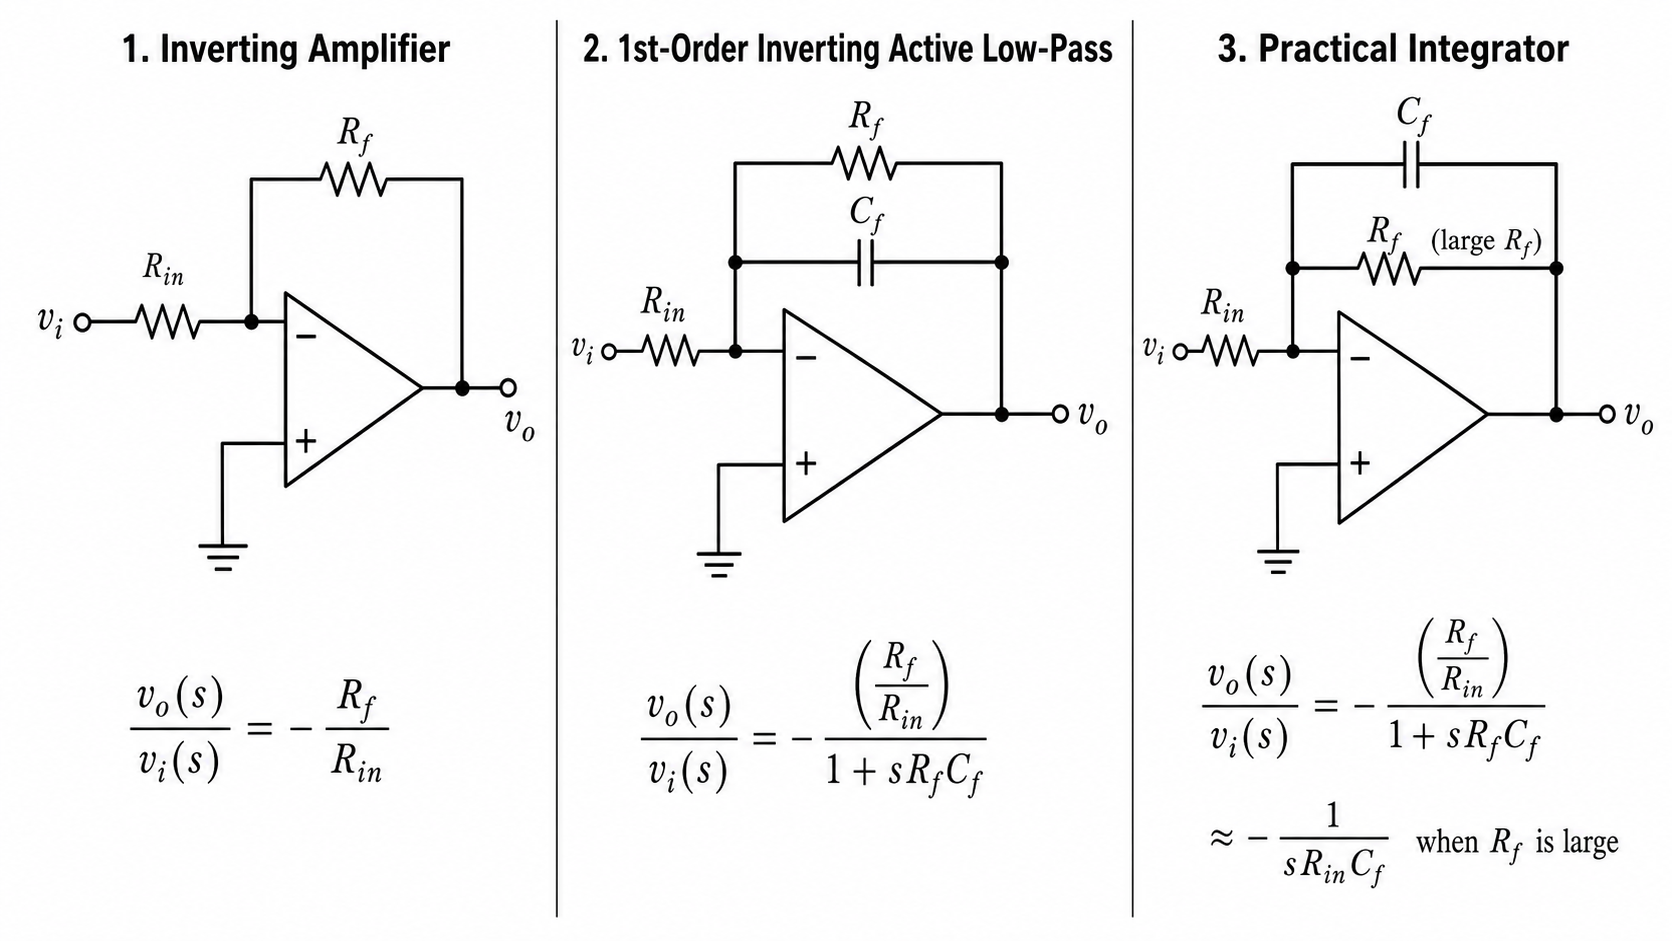
\includegraphics[width=0.8\textwidth]{images/chapter3/figure-6.png}
    \caption{วงจร Op-Amp และฟังก์ชันถ่ายโอน}
\end{figure}

\paragraph{7.5.6 ข้อจำกัดของแบบจำลองวงจรอุดมคติ}

แบบจำลองข้างต้นอาจคลาดเคลื่อนเมื่อ

\begin{itemize}
    \item ตัวต้านทาน ตัวเก็บประจุ และตัวเหนี่ยวนำมีค่าคลาดเคลื่อน
    \item ตัวเหนี่ยวนำมีความต้านทานขดลวดและความจุแฝง
    \item ตัวเก็บประจุมี ESR และการรั่วไหล
    \item เครื่องกำเนิดสัญญาณมีความต้านทานเอาต์พุต
    \item Oscilloscope และหัววัดเพิ่มโหลดให้วงจร
    \item Op-Amp มี gain-bandwidth product, slew rate, input bias current และข้อจำกัดแรงดันเอาต์พุต
    \item ระบบเข้าสู่ช่วงไม่เชิงเส้น เช่น Op-Amp อิ่มตัวหรือแกนอิ่มตัวของตัวเหนี่ยวนำ
\end{itemize}

การเลือกความละเอียดของแบบจำลองจึงต้องสัมพันธ์กับวัตถุประสงค์ หากใช้ศึกษาพฤติกรรมพื้นฐาน แบบจำลองอุดมคติอาจเพียงพอ แต่หากต้องการให้ผลจำลองใกล้ผลทดลอง ต้องรวมพารามิเตอร์แฝงที่สำคัญ

\subsubsection{7.6 การสร้างแบบจำลองระบบไฟฟ้า–กล: มอเตอร์กระแสตรง}

มอเตอร์กระแสตรง (DC Motor) เป็นตัวอย่างสำคัญของระบบไฟฟ้า–กล (University of Michigan, n.d.) เนื่องจากมีการเปลี่ยนพลังงานไฟฟ้าที่ขดลวดอาร์เมเจอร์เป็นแรงบิดและการเคลื่อนที่เชิงหมุน แบบจำลองต้องเชื่อมสมการวงจรไฟฟ้าเข้ากับสมการกลศาสตร์

\paragraph{7.6.1 ตัวแปรและพารามิเตอร์}

\begin{table}[htbp]
    \centering
    \begin{tabular}{l l l}
        \hline
        \textbf{สัญลักษณ์} & \textbf{ความหมาย} & \textbf{หน่วย} \\
        \hline
        $v_a(t)$ & แรงดันอาร์เมเจอร์ & V \\
        $i_a(t)$ & กระแสอาร์เมเจอร์ & A \\
        $R_a$ & ความต้านทานอาร์เมเจอร์ & $\Omega$ \\
        $L_a$ & ความเหนี่ยวนำอาร์เมเจอร์ & H \\
        $e_b(t)$ & แรงดันต้านกลับ (Back EMF) & V \\
        $K_e$ & ค่าคงตัวแรงดันต้านกลับ & V·s/rad \\
        $T_m(t)$ & แรงบิดแม่เหล็กไฟฟ้า & N·m \\
        $K_t$ & ค่าคงตัวแรงบิด & N·m/A \\
        $J$ & โมเมนต์ความเฉื่อยรวมที่เพลา & kg·m$^2$ \\
        $b$ & สัมประสิทธิ์แรงเสียดทานหนืด & N·m·s/rad \\
        $\theta(t)$ & ตำแหน่งเชิงมุม & rad \\
        $\omega(t)=\dot{\theta}(t)$ & ความเร็วเชิงมุม & rad/s \\
        $T_L(t)$ & แรงบิดโหลดรบกวน & N·m \\
        \hline
    \end{tabular}
\end{table}

สำหรับหน่วย SI มักมีค่าตัวเลข $K_t=K_e=K$ แต่มีหน่วยต่างกันและมีความหมายทางกายภาพต่างกัน

\paragraph{7.6.2 สมการส่วนไฟฟ้า}

จาก KVL ที่วงจรอาร์เมเจอร์

\[
v_a(t)=L_a\frac{di_a(t)}{dt}+R_ai_a(t)+e_b(t)
\]

แรงดันต้านกลับแปรผันกับความเร็ว

\[
e_b(t)=K_e\omega(t)
\]

จึงได้

\[
L_a\frac{di_a(t)}{dt}+R_ai_a(t)+K_e\omega(t)=v_a(t)
\]

\paragraph{7.6.3 สมการส่วนกล}

แรงบิดแม่เหล็กไฟฟ้าเป็น

\[
T_m(t)=K_ti_a(t)
\]

สมดุลแรงบิดที่เพลาเมื่อรวมแรงบิดโหลด

\[
J\frac{d\omega(t)}{dt}+b\omega(t)=K_ti_a(t)-T_L(t)
\]

สำหรับการหาฟังก์ชันถ่ายโอนจากแรงดันอาร์เมเจอร์ไปยังความเร็ว ให้กำหนด $T_L(t)=0$

\paragraph{7.6.4 การหาฟังก์ชันถ่ายโอนความเร็ว}

แปลงลาปลาซภายใต้ค่าเริ่มต้นเป็นศูนย์

\[
(L_as+R_a)I_a(s)+K_e\Omega(s)=V_a(s)
\]

\[
(Js+b)\Omega(s)=K_tI_a(s)
\]

จากสมการกล

\[
I_a(s)=\frac{Js+b}{K_t}\Omega(s)
\]

แทนในสมการไฟฟ้า

\[
\left[
\frac{(L_as+R_a)(Js+b)}{K_t}+K_e
\right]\Omega(s)=V_a(s)
\]

จึงได้

\[
\boxed{
\frac{\Omega(s)}{V_a(s)}
=
\frac{K_t}
{(L_as+R_a)(Js+b)+K_tK_e}
}
\]

ขยายพหุนามส่วน

\[
\boxed{
\frac{\Omega(s)}{V_a(s)}
=
\frac{K_t}
{L_aJs^2+(L_ab+R_aJ)s+(R_ab+K_tK_e)}
}
\]

ฟังก์ชันถ่ายโอนตำแหน่งได้จาก $\Omega(s)=s\Theta(s)$

\[
\boxed{
\frac{\Theta(s)}{V_a(s)}
=
\frac{K_t}
{s\left[L_aJs^2+(L_ab+R_aJ)s+(R_ab+K_tK_e)\right]}
}
\]

หากละเลย $L_a$ เพราะค่าคงตัวเวลาทางไฟฟ้า $L_a/R_a$ เล็กกว่าค่าคงตัวเวลาทางกลมาก แบบจำลองความเร็วจะลดเป็นระบบอันดับหนึ่ง

\[
\frac{\Omega(s)}{V_a(s)}
\approx
\frac{K_t}
{R_aJs+(R_ab+K_tK_e)}
\]

อย่างไรก็ตาม การละเลย $L_a$ ต้องอาศัยเหตุผลจากขนาดพารามิเตอร์และช่วงความถี่ที่สนใจ ไม่ควรละเลยโดยอัตโนมัติ

% [รูปที่ 7: แบบจำลองเชื่อมโยงพลังงานของมอเตอร์ DC]
% ประเภทภาพ: Electromechanical Block Diagram / Technical Illustration
% ตำแหน่งที่แนะนำ: หัวข้อ 7.6
% วัตถุประสงค์การเรียนรู้: แสดงการเชื่อมโยงระหว่างแรงดัน กระแส แรงบิด และความเร็ว รวมทั้งป้อนกลับภายในจาก Back EMF
% คำอธิบายภาพ: แผนภาพพลังงานจากแรงดันอาร์เมเจอร์เข้าสู่วงจร $R_a$–$L_a$ ได้กระแส $i_a$ ผ่านค่าคงตัว $K_t$ เป็นแรงบิด ขับระบบกล $1/(Js+b)$ เป็นความเร็ว และความเร็วผ่าน $K_e$ ป้อนกลับลบเป็น Back EMF
% องค์ประกอบที่ต้องมี: จุดรวมสัญญาณ, $V_a(s)$, $I_a(s)$, $K_t$, $T_m(s)$, $1/(Js+b)$, $\Omega(s)$, $K_e$, $E_b(s)$, แรงบิดโหลด $T_L(s)$
% ข้อความหรือป้ายกำกับ: “Armature Circuit”, “Torque Constant”, “Mechanical Dynamics”, “Back EMF”, “Load Torque”
% ภาษาของป้ายกำกับ: อังกฤษ
% สัดส่วนภาพ: 16:9
% Image Generation Prompt: Accurate educational block diagram of an armature-controlled DC motor. Input Va(s) enters a summing junction subtracting back EMF Eb(s), then block 1/(La s + Ra) produces armature current Ia(s). Block Kt produces electromagnetic torque Tm(s). A second summing junction subtracts load torque TL(s), then block 1/(J s + b) produces angular speed Omega(s). Feedback from Omega(s) through Ke returns as Eb(s) to the first summing junction. Blue forward path, orange internal feedback, red disturbance arrow, white background, control engineering textbook style.
% Alt Text: แผนภาพบล็อกมอเตอร์ DC แสดงวงจรอาร์เมเจอร์ การสร้างแรงบิด ระบบกล และแรงดันต้านกลับ

\begin{figure}[htbp]
    \centering
    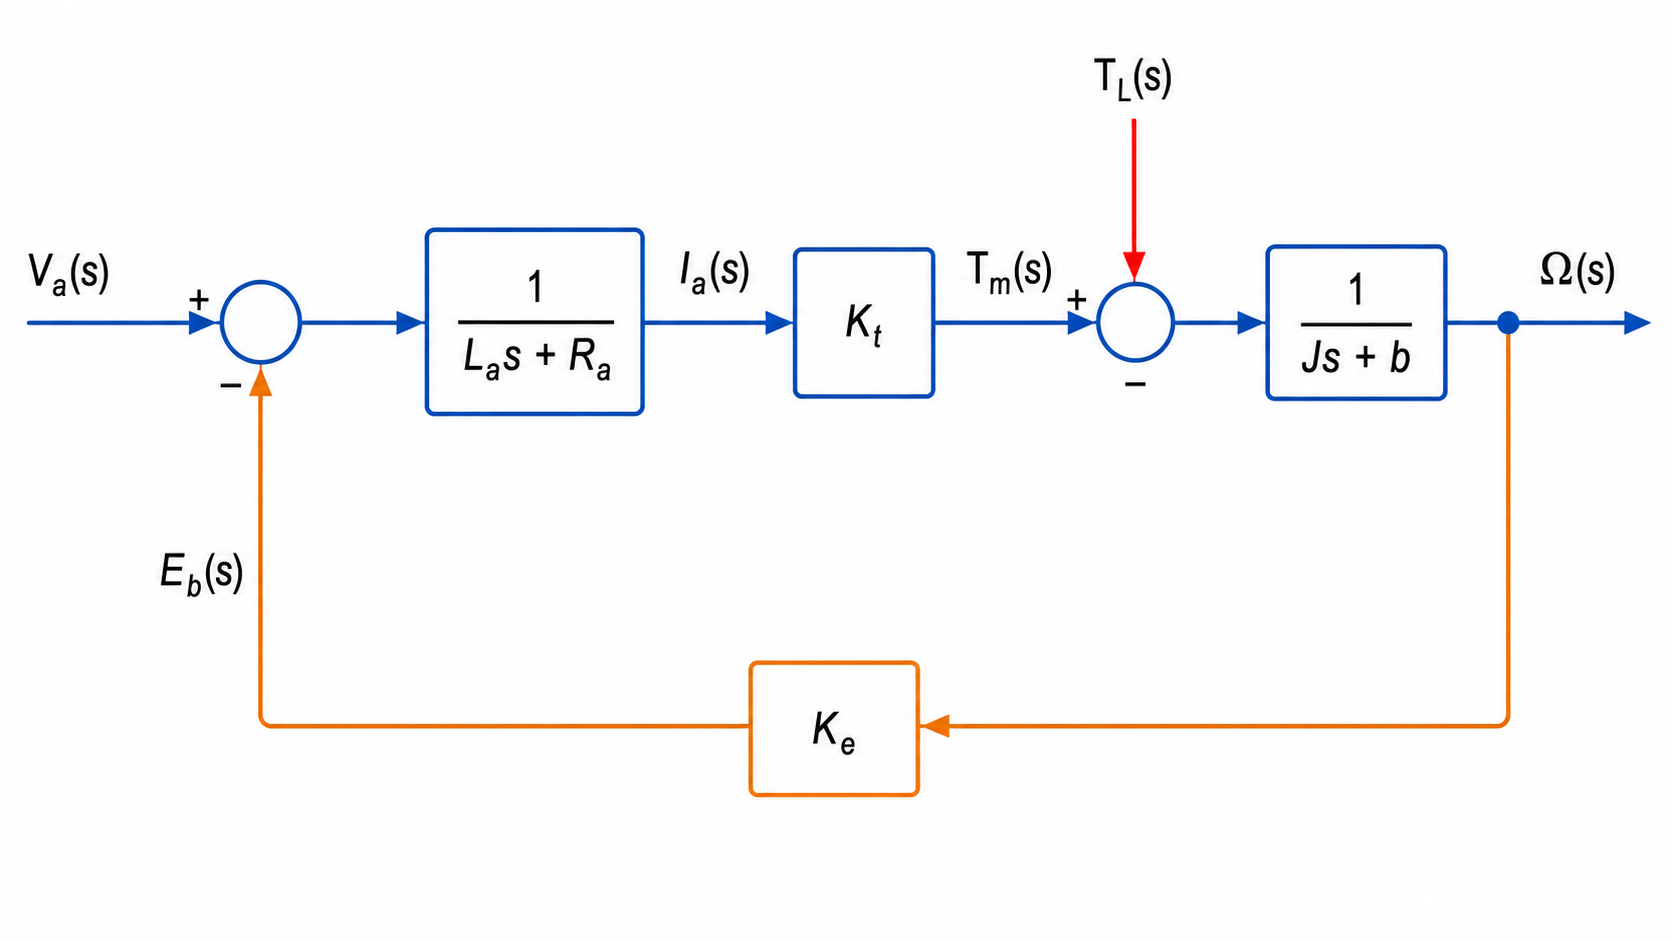
\includegraphics[width=0.8\textwidth]{images/chapter3/figure-7.png}
    \caption{แบบจำลองเชื่อมโยงพลังงานของมอเตอร์ DC}
\end{figure}

\paragraph{7.6.5 ตัวอย่างบังคับ: แบบจำลองมอเตอร์ DC}

\textbf{ตัวอย่างเพิ่มเติมเพื่อการเรียนรู้}\\กำหนด

\[
J=0.01\ \text{kg·m}^2,\quad
b=0.1\ \text{N·m·s/rad}
\]

\[
K_t=K_e=0.01,\quad
R_a=1\ \Omega,\quad
L_a=0.5\ \text{H}
\]

ต้องการฟังก์ชันถ่ายโอนจาก $V_a(s)$ ไปยัง $\Omega(s)$ เมื่อไม่มีแรงบิดโหลดรบกวน

\textbf{1. เลือกสมการทั่วไป}

\[
\frac{\Omega(s)}{V_a(s)}
=
\frac{K_t}
{L_aJs^2+(L_ab+R_aJ)s+(R_ab+K_tK_e)}
\]

\textbf{2. คำนวณสัมประสิทธิ์}

\[
L_aJ=(0.5)(0.01)=0.005
\]

\[
L_ab+R_aJ=(0.5)(0.1)+(1)(0.01)=0.06
\]

\[
R_ab+K_tK_e=(1)(0.1)+(0.01)(0.01)=0.1001
\]

\textbf{3. เขียนฟังก์ชันถ่ายโอน}

\[
\boxed{
\frac{\Omega(s)}{V_a(s)}
=
\frac{0.01}{0.005s^2+0.06s+0.1001}
}
\]

หารทั้งเศษและส่วนด้วย $0.005$

\[
\boxed{
\frac{\Omega(s)}{V_a(s)}
=
\frac{2}{s^2+12s+20.02}
}
\]

\textbf{4. วิเคราะห์โพล}

รากของส่วนมีค่าประมาณ

\[
p_1\approx-2.0025,\qquad
p_2\approx-9.9975
\]

โพลทั้งสองอยู่ซีกซ้ายของระนาบเชิงซ้อน จึงเป็นแบบจำลองที่เสถียร โพลที่อยู่ใกล้จุดกำเนิดกว่าคือ $p_1$ มีอิทธิพลต่อพฤติกรรมช้ามากกว่า

\textbf{5. ตรวจสอบอัตราขยายสภาวะคงตัว}

\[
G(0)=\frac{0.01}{0.1001}
\approx0.0999\ \frac{\text{rad/s}}{\text{V}}
\]

หากป้อนแรงดันคงที่ $10\ \text{V}$ แบบจำลองทำนายความเร็วสภาวะคงตัวประมาณ

\[
\omega_{ss}\approx0.999\ \text{rad/s}
\]

ค่าตัวเลขตัวอย่างนี้ใช้เพื่อฝึกกระบวนการสร้างแบบจำลอง ไม่ได้แทนมอเตอร์ชนิดใดโดยเฉพาะ

\paragraph{7.6.6 แบบจำลองที่มีแรงบิดโหลดเป็นอินพุตรบกวน}

เมื่อเก็บ $T_L(s)$ ไว้ จะได้ระบบสองอินพุต

\[
\Omega(s)
=
G_v(s)V_a(s)+G_d(s)T_L(s)
\]

โดย

\[
G_v(s)=
\frac{K_t}
{(L_as+R_a)(Js+b)+K_tK_e}
\]

และ

\[
G_d(s)=
-\frac{L_as+R_a}
{(L_as+R_a)(Js+b)+K_tK_e}
\]

เครื่องหมายลบแสดงว่าแรงบิดโหลดที่ต้านการหมุนทำให้ความเร็วลดลง การแยกเส้นทางอินพุตควบคุมและอินพุตรบกวนมีประโยชน์ต่อการวิเคราะห์ระบบควบคุมในบทถัดไป

\par\noindent\rule{\textwidth}{0.4pt}\par

\subsubsection{7.7 การเขียนสมการสถานะเบื้องต้นจาก Transfer Function}

ฟังก์ชันถ่ายโอนอธิบายความสัมพันธ์อินพุต–เอาต์พุต แต่ไม่แสดงตัวแปรภายในโดยตรง แบบจำลองปริภูมิสถานะ (State-Space Model) เขียนในรูป

\[
\dot{\mathbf{x}}(t)=A\mathbf{x}(t)+B\mathbf{u}(t)
\]

\[
\mathbf{y}(t)=C\mathbf{x}(t)+D\mathbf{u}(t)
\]

โดย

\begin{itemize}
    \item $\mathbf{x}(t)$ คือเวกเตอร์สถานะ
    \item $\mathbf{u}(t)$ คือเวกเตอร์อินพุต
    \item $\mathbf{y}(t)$ คือเวกเตอร์เอาต์พุต
    \item $A$ คือเมทริกซ์พลวัตของระบบ
    \item $B$ คือเมทริกซ์อินพุต
    \item $C$ คือเมทริกซ์เอาต์พุต
    \item $D$ คือเมทริกซ์ส่งผ่านโดยตรง
\end{itemize}

สำหรับระบบ LTI ที่มีค่าเริ่มต้นเป็นศูนย์ ความสัมพันธ์กับฟังก์ชันถ่ายโอนคือ

\[
\boxed{
G(s)=C(sI-A)^{-1}B+D
}
\]

แบบจำลองสถานะของฟังก์ชันถ่ายโอนหนึ่งชุด \textbf{ไม่เป็นเอกลักษณ์} (Massachusetts Institute of Technology OpenCourseWare, n.d.) กล่าวคือ มีเมทริกซ์ $A,B,C,D$ ได้หลายชุดที่ให้ความสัมพันธ์อินพุต–เอาต์พุตเดียวกัน หากสถานะถูกแปลงด้วยเมทริกซ์ไม่เอกฐาน ระบบใหม่ยังคงมีฟังก์ชันถ่ายโอนเดิม

\paragraph{7.7.1 รูป Canonical สำหรับระบบอันดับสอง}

ให้

\[
G(s)=\frac{b_1s+b_0}{s^2+a_1s+a_0}
\]

รูป Controllable Canonical Form หนึ่งรูปคือ

\[
A=
\begin{bmatrix}
0 & 1\\
-a_0 & -a_1
\end{bmatrix},
\qquad
B=
\begin{bmatrix}
0\\
1
\end{bmatrix}
\]

\[
C=
\begin{bmatrix}
b_0 & b_1
\end{bmatrix},
\qquad
D=0
\]

ตรวจสอบได้จาก $G(s)=C(sI-A)^{-1}B$

หากเศษมีดีกรีเท่ากับส่วน ต้องแยกพจน์ส่งผ่านโดยตรง $D$ ก่อน เพื่อให้ส่วนที่เหลือเป็นฟังก์ชันถ่ายโอน proper

\paragraph{7.7.2 ตัวอย่าง: แปลง Transfer Function ของระบบกลเป็น State Equation}

จากตัวอย่างระบบมวล–สปริง–ตัวหน่วง

\[
G(s)=\frac{X(s)}{F(s)}
=\frac{1}{2s^2+6s+8}
=\frac{0.5}{s^2+3s+4}
\]

ดังนั้น

\[
a_1=3,\quad a_0=4,\quad b_1=0,\quad b_0=0.5
\]

รูป Canonical คือ

\[
A=
\begin{bmatrix}
0 & 1\\
-4 & -3
\end{bmatrix},
\quad
B=
\begin{bmatrix}
0\\
1
\end{bmatrix}
\]

\[
C=
\begin{bmatrix}
0.5 & 0
\end{bmatrix},
\quad
D=0
\]

อีกวิธีหนึ่งคือเลือกสถานะทางกายภาพ

\[
x_1=x,\qquad x_2=\dot{x}
\]

จาก

\[
2\ddot{x}+6\dot{x}+8x=F
\]

จะได้

\[
\dot{x}_1=x_2
\]

\[
\dot{x}_2=-4x_1-3x_2+0.5F
\]

ดังนั้น

\[
A=
\begin{bmatrix}
0 & 1\\
-4 & -3
\end{bmatrix},
\quad
B=
\begin{bmatrix}
0\\
0.5
\end{bmatrix}
\]

\[
C=
\begin{bmatrix}
1 & 0
\end{bmatrix},
\quad
D=0
\]

ทั้งสอง realization ให้ฟังก์ชันถ่ายโอนเดียวกัน แต่ความหมายของสถานะต่างกัน รูปที่ใช้สถานะทางกายภาพมักตีความได้ง่ายกว่า ส่วนรูป canonical สร้างจากสัมประสิทธิ์พหุนามได้โดยตรง

% [รูปที่ 8: เปรียบเทียบ Transfer Function และ State-Space Realization]
% ประเภทภาพ: Conceptual Block Diagram
% ตำแหน่งที่แนะนำ: หัวข้อ 7.7
% วัตถุประสงค์การเรียนรู้: แสดงว่าฟังก์ชันถ่ายโอนเดียวกันสามารถมีการเลือกสถานะหลายแบบ
% คำอธิบายภาพ: ด้านซ้ายเป็นกล่อง $G(s)$ เชื่อมอินพุต $u$ กับเอาต์พุต $y$ ด้านขวาแตกแขนงเป็น realization สองแบบ ได้แก่ canonical states และ physical states โดยลูกศรทั้งสองย้อนกลับมาที่ฟังก์ชันถ่ายโอนเดียวกัน
% องค์ประกอบที่ต้องมี: $u(t)$, $y(t)$, $G(s)$, $A,B,C,D$, canonical states, physical states, ลูกศร similarity transformation
% ข้อความหรือป้ายกำกับ: “Input–Output Model”, “Internal-State Model”, “Non-unique Realizations”, “Same Transfer Function”
% ภาษาของป้ายกำกับ: อังกฤษ
% สัดส่วนภาพ: 16:9
% Image Generation Prompt: Educational control-systems diagram comparing a transfer-function input-output model with two state-space realizations. Left: u(t) enters a block G(s) and produces y(t). Right: two parallel boxes labeled Controllable Canonical States and Physical States, each containing A, B, C, D matrices; arrows indicate both produce the same G(s), with a similarity transformation arrow between the realizations. Clean academic vector style, white background, blue and gray accents.
% Alt Text: ฟังก์ชันถ่ายโอนหนึ่งชุดเชื่อมโยงกับแบบจำลองสถานะได้หลายรูปแบบที่ให้ผลอินพุต–เอาต์พุตเดียวกัน

\begin{figure}[htbp]
    \centering
    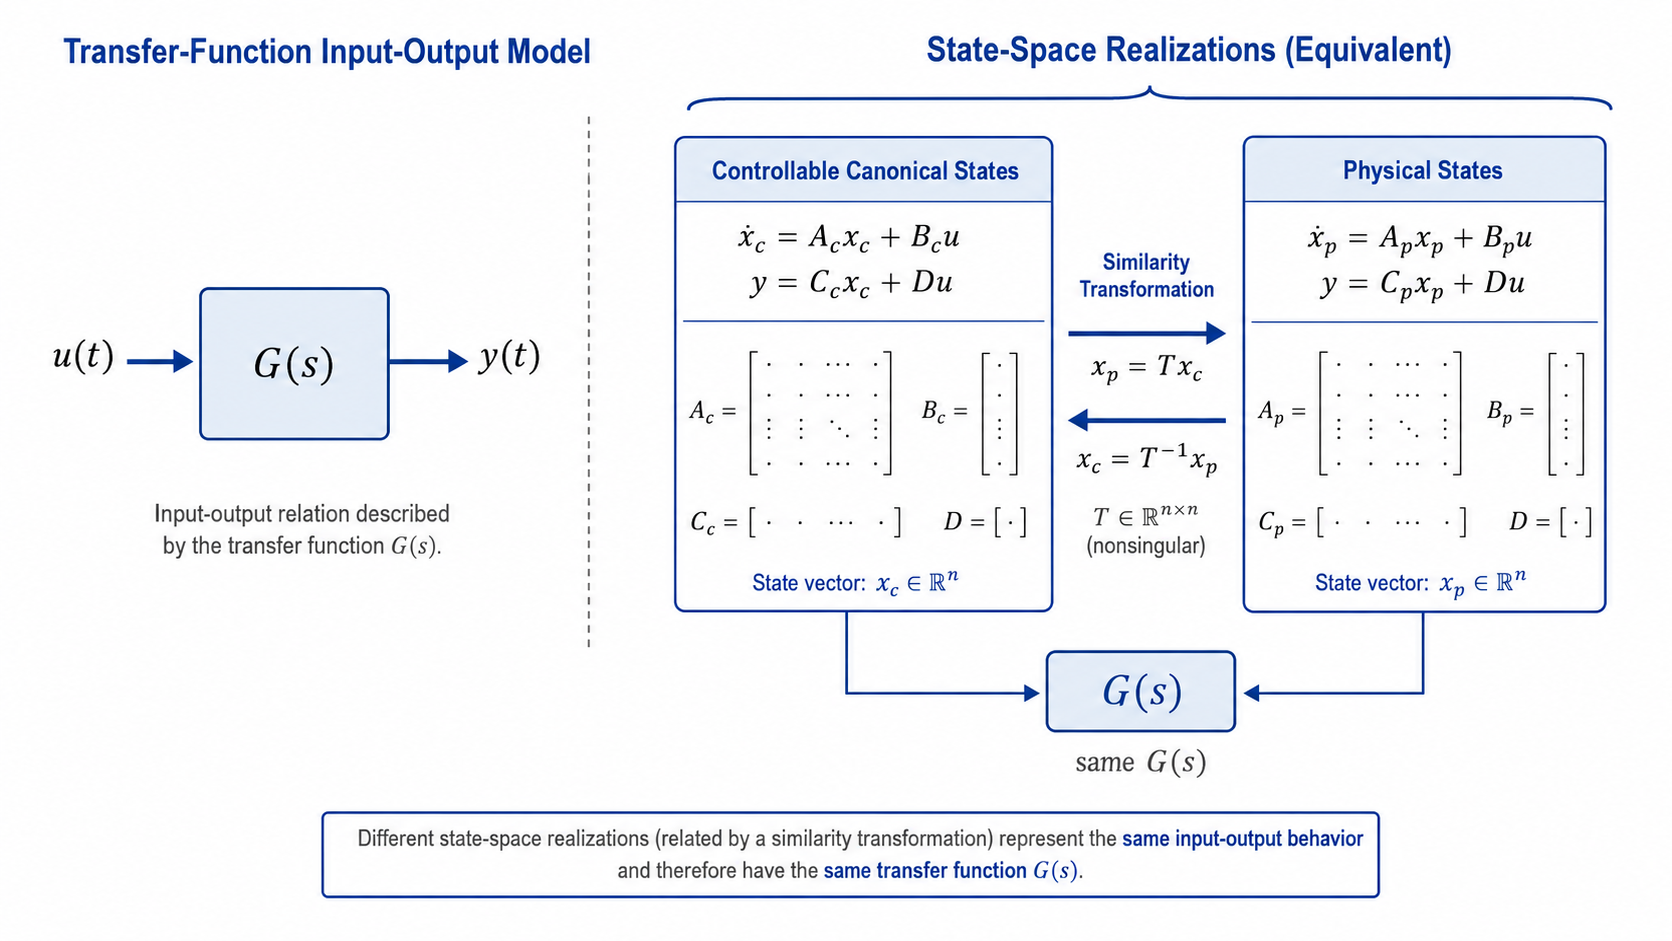
\includegraphics[width=0.8\textwidth]{images/chapter3/figure-8.png}
    \caption{เปรียบเทียบ Transfer Function และ State-Space Realization}
\end{figure}

\par\noindent\rule{\textwidth}{0.4pt}\par

\subsubsection{7.8 การตรวจสอบและยืนยันแบบจำลอง}

การได้สมการไม่ใช่จุดสิ้นสุดของการสร้างแบบจำลอง ควรตรวจสอบอย่างน้อยสี่ระดับ

\paragraph{7.8.1 ตรวจสอบโครงสร้างและหน่วย}

\begin{itemize}
    \item สมการทุกพจน์ต้องมีหน่วยเดียวกัน
    \item อันดับของระบบควรสัมพันธ์กับจำนวนองค์ประกอบสะสมพลังงานอิสระ
    \item เครื่องหมายของแรง แรงบิด แรงดัน และกระแสต้องสอดคล้องกับทิศทางอ้างอิง
    \item ฟังก์ชันถ่ายโอนของระบบกายภาพทั่วไปควรเป็น proper เว้นแต่มีเหตุผลเฉพาะ
\end{itemize}

\paragraph{7.8.2 ตรวจสอบกรณีขอบเขต}

ตัวอย่างเช่น

\begin{itemize}
    \item $s\rightarrow0$ แสดงพฤติกรรมสภาวะคงตัว
    \item $s\rightarrow\infty$ แสดงแนวโน้มความถี่สูง
    \item $R\rightarrow0$, $C\rightarrow0$, $m\rightarrow0$ หรือพารามิเตอร์อื่นควรให้พฤติกรรมที่มีเหตุผล
    \item เมื่อไม่มีการหน่วง ระบบควรสะท้อนการสั่นตามธรรมชาติที่เหมาะสม
\end{itemize}

\paragraph{7.8.3 ตรวจสอบด้วยการจำลอง}

เปรียบเทียบ

\begin{enumerate}
    \item ผลจากสมการเชิงอนุพันธ์
    \item ผลจาก Transfer Function
    \item ผลจาก State-Space
    \item ผลจาก Simulink
\end{enumerate}

สำหรับอินพุตและค่าเริ่มต้นเดียวกัน ผลควรสอดคล้องกันภายในความคลาดเคลื่อนเชิงตัวเลข

\paragraph{7.8.4 ตรวจสอบกับข้อมูลทดลอง}

ใช้ตัวชี้วัด เช่น

\[
\%\text{Error}
=
\left|
\frac{x_{\text{measured}}-x_{\text{model}}}
{x_{\text{model}}}
\right|\times100
\]

สำหรับข้อมูลหลายจุด อาจใช้ค่าเฉลี่ยความคลาดเคลื่อนสัมบูรณ์

\[
\text{MAE}
=
\frac{1}{N}\sum_{k=1}^{N}
|y_k-\hat{y}_k|
\]

ความคลาดเคลื่อนไม่ได้หมายความว่าแบบจำลอง “ผิด” เสมอไป แต่อาจบ่งชี้ว่า

\begin{itemize}
    \item พารามิเตอร์จริงต่างจากค่าป้ายกำกับ
    \item มีไดนามิกที่ละเลย
    \item เครื่องมือวัดและการสุ่มตัวอย่างมีข้อจำกัด
    \item ระบบมีสัญญาณรบกวนหรือไม่เชิงเส้น
    \item จุดทำงานของระบบเปลี่ยนไป
\end{itemize}

\par\noindent\rule{\textwidth}{0.4pt}\par

\subsection{8. การใช้ MATLAB และ Simulink เพื่อสร้างและตรวจสอบแบบจำลอง}

\subsubsection{8.1 วัตถุประสงค์}

หลังจากศึกษาส่วนนี้ นักศึกษาควรสามารถ

\begin{enumerate}
    \item สร้างวัตถุ Transfer Function จากสัมประสิทธิ์เศษและส่วน
    \item ตรวจสอบโพล ซีโร และการตอบสนองขั้นบันได
    \item แปลง Transfer Function เป็น State-Space
    \item สร้างแบบจำลองบล็อกใน Simulink
    \item เปรียบเทียบผลคำนวณ ผลจำลอง และผลทดลอง
\end{enumerate}

\begin{quote}
\textbf{หมายเหตุด้านเวอร์ชัน:} ชื่อคำสั่งและบล็อกต่อไปนี้เป็นชื่อมาตรฐานที่ใช้ทั่วไปใน MATLAB/Simulink แต่หน้าตาเมนูอาจแตกต่างตามเวอร์ชันและผลิตภัณฑ์เสริมที่ติดตั้ง
\end{quote}

\subsubsection{8.2 MATLAB: ระบบมวล–สปริง–ตัวหน่วง}

\begin{verbatim}
% Mass-spring-damper parameters
m = 2;      % kg
c = 6;      % N*s/m
k = 8;      % N/m

% G(s) = X(s)/F(s)
num_msd = 1;
den_msd = [m c k];
G_msd = tf(num_msd, den_msd);

disp(G_msd)
pole(G_msd)
zero(G_msd)

figure
step(G_msd)
grid on
title('Step response: Mass-Spring-Damper')
xlabel('Time (s)')
ylabel('Displacement (m) for 1-N step force')
\end{verbatim}

\textbf{สิ่งที่ควรสังเกต}

\begin{itemize}
    \item สัมประสิทธิ์ใน \texttt{den\_msd} เรียงตามกำลังของ $s$ จากมากไปน้อย
    \item การตอบสนองต่อแรงขั้นบันไดขนาด $1\ \text{N}$ ควรเข้าสู่ $1/k=0.125\ \text{m}$
    \item โพลต้องตรงกับรากของ $2s^2+6s+8$
\end{itemize}

\subsubsection{8.3 MATLAB: วงจร RLC}

\begin{verbatim}
R = 100;        % ohm
L = 10e-3;      % H
C = 1e-6;       % F

% G(s) = Vc(s)/Vin(s)
num_rlc = 1;
den_rlc = [L*C R*C 1];
G_rlc = tf(num_rlc, den_rlc);

figure
step(G_rlc)
grid on
title('Step response: Series RLC, output across C')
xlabel('Time (s)')
ylabel('Normalized capacitor voltage')

figure
bode(G_rlc)
grid on
\end{verbatim}

สำหรับแบบจำลองเชิงปฏิบัติ ให้แทน \texttt{R} ด้วย $R_{\text{eq}}$ ที่รวมความต้านทานแหล่งกำเนิดและขดลวด

\begin{verbatim}
Rs = 50;        % source resistance, ohm
rL = 20;        % measured inductor winding resistance, ohm
Req = R + Rs + rL;

G_rlc_practical = tf(1, [L*C Req*C 1]);

figure
bode(G_rlc, G_rlc_practical)
grid on
legend('Ideal', 'Practical')
\end{verbatim}

\subsubsection{8.4 MATLAB: มอเตอร์ DC}

\begin{verbatim}
J  = 0.01;      % kg*m^2
b  = 0.1;       % N*m*s/rad
Kt = 0.01;      % N*m/A
Ke = 0.01;      % V*s/rad
Ra = 1;         % ohm
La = 0.5;       % H

num_motor = Kt;
den_motor = [La*J, La*b + Ra*J, Ra*b + Kt*Ke];

G_motor = tf(num_motor, den_motor);

disp(G_motor)
pole(G_motor)
dcgain(G_motor)

figure
step(G_motor)
grid on
title('DC Motor Speed Response')
xlabel('Time (s)')
ylabel('Angular speed (rad/s) for 1-V step')
\end{verbatim}

\subsubsection{8.5 แปลง Transfer Function เป็น State-Space}

\begin{verbatim}
[A, B, Cmat, D] = tf2ss(num_msd, den_msd);

disp(A)
disp(B)
disp(Cmat)
disp(D)

sys_ss = ss(A, B, Cmat, D);

figure
step(G_msd, sys_ss)
grid on
legend('Transfer Function', 'State Space')
title('Comparison of equivalent realizations')
\end{verbatim}

ผลการตอบสนองอินพุต–เอาต์พุตควรซ้อนกัน แต่ค่าของสถานะภายในอาจไม่ตรงกับตำแหน่งและความเร็วทางกายภาพ เนื่องจาก \texttt{tf2ss} สร้าง realization ตามรูปแบบเชิงคำนวณ

\subsubsection{8.6 การสร้างแบบจำลองใน Simulink}

\paragraph{8.6.1 บล็อกที่ใช้}

\begin{itemize}
    \item \textbf{Step}: สร้างอินพุตขั้นบันได
    \item \textbf{Transfer Fcn}: ป้อนสัมประสิทธิ์เศษและส่วน
    \item \textbf{Scope}: แสดงสัญญาณเวลา
    \item \textbf{To Workspace}: ส่งข้อมูลไปวิเคราะห์ใน MATLAB
    \item \textbf{Mux}: รวมสัญญาณเพื่อเปรียบเทียบ
    \item \textbf{Sum}, \textbf{Gain}, \textbf{Integrator}: ใช้สร้างแบบจำลองจากสมการสถานะหรือสมการเชิงอนุพันธ์
\end{itemize}

\paragraph{8.6.2 แบบจำลอง RLC ด้วย Transfer Fcn}

\begin{enumerate}
    \item วางบล็อก \texttt{Step}
    \item ต่อเข้าบล็อก \texttt{Transfer Fcn}
    \item กำหนด Numerator เป็น \texttt{[1]}
    \item กำหนด Denominator เป็น \texttt{[L*C R*C 1]} หรือใส่ค่าตัวเลข \texttt{[1e-8 1e-4 1]}
    \item ต่อเอาต์พุตเข้าบล็อก \texttt{Scope}
    \item กำหนด Stop Time ให้ครอบคลุมหลายคาบของพลวัต เช่น \texttt{0.005} s
    \item รันแบบจำลองและอ่านค่า overshoot, rise time และ settling behavior
\end{enumerate}

\paragraph{8.6.3 แบบจำลอง RLC จาก Integrator}

จาก

\[
LC\ddot{v}_o+RC\dot{v}_o+v_o=v_i
\]

จัดรูป

\[
\ddot{v}_o
=
\frac{1}{LC}v_i
-\frac{R}{L}\dot{v}_o
-\frac{1}{LC}v_o
\]

ใช้ Integrator สองตัวต่ออนุกรมเพื่อสร้าง $\dot{v}_o$ และ $v_o$ แล้วป้อนกลับทั้งสองสัญญาณผ่าน Gain ที่เหมาะสม วิธีนี้ทำให้เห็นโครงสร้างสถานะของระบบโดยตรง

% [รูปที่ 9: แบบจำลอง Simulink ของวงจร RLC สองแนวทาง]
% ประเภทภาพ: Software Block Diagram
% ตำแหน่งที่แนะนำ: หัวข้อ 8.6
% วัตถุประสงค์การเรียนรู้: เปรียบเทียบการจำลองด้วยบล็อก Transfer Fcn กับการสร้างจากสมการเชิงอนุพันธ์
% คำอธิบายภาพ: ด้านบนเป็น Step → Transfer Fcn → Scope ด้านล่างเป็น Sum ต่อ Integrator สองตัว พร้อม Gain ป้อนกลับจาก $v_o$ และ $\dot{v}_o$ โดยเอาต์พุตทั้งสองแนวทางเข้า Mux และ Scope เดียวกัน
% องค์ประกอบที่ต้องมี: Step, Transfer Fcn, Sum, Gain, Integrator สองตัว, Mux, Scope, ป้าย $v_i$, $\dot{v}_o$, $v_o$
% ข้อความหรือป้ายกำกับ: “Transfer-Function Model”, “Differential-Equation Model”, “Compare Outputs”
% ภาษาของป้ายกำกับ: อังกฤษ
% สัดส่วนภาพ: 16:9
% Image Generation Prompt: MATLAB Simulink-style educational block diagram comparing two equivalent series RLC models. Top path: Step block to Transfer Fcn block with numerator [1] and denominator [LC RC 1], then Scope. Bottom path: Step enters a summing block that also receives negative feedback from vo and vo-dot through gains; output drives two cascaded Integrator blocks to produce vo-dot and vo. Feed both model outputs through a Mux into one Scope. Use authentic generic block-diagram appearance without software logos, clear signal labels, white canvas.
% Alt Text: แบบจำลอง RLC ใน Simulink โดยใช้ Transfer Fcn และ Integrator สองตัวเพื่อเปรียบเทียบผล

\begin{figure}[htbp]
    \centering
    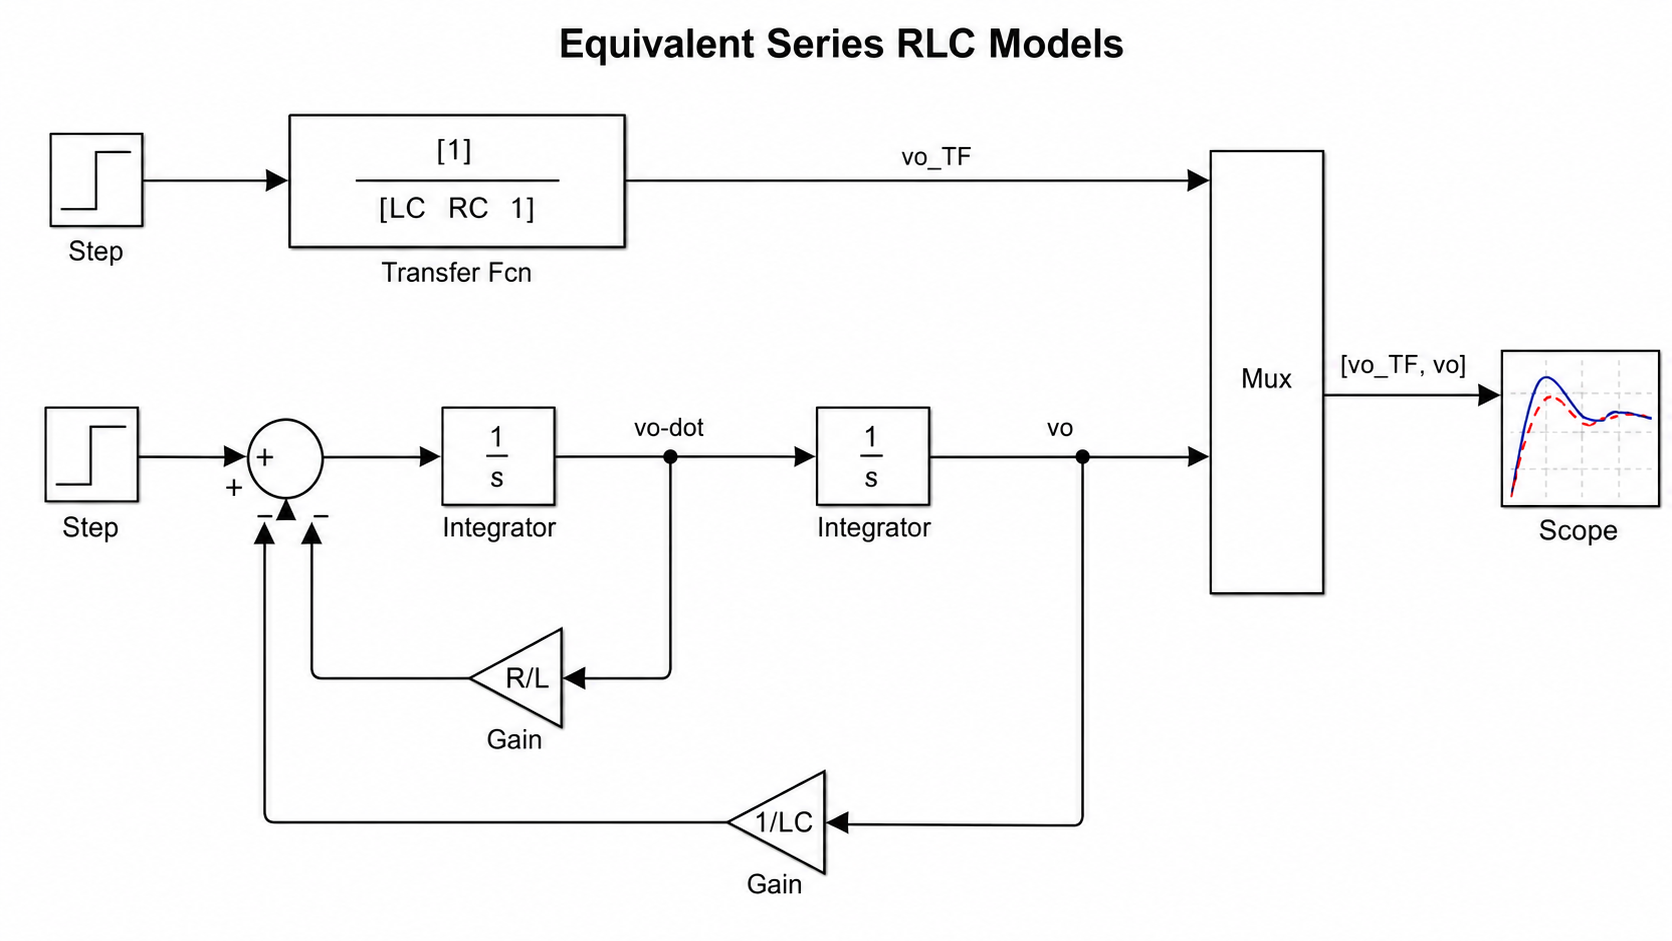
\includegraphics[width=0.8\textwidth]{images/chapter3/figure-9.png}
    \caption{แบบจำลอง Simulink ของวงจร RLC สองแนวทาง}
\end{figure}

\subsubsection{8.7 ผลลัพธ์ที่คาดหวังและวิธีอ่านผล}

\begin{itemize}
    \item กราฟ RLC จากสองแบบจำลองควรซ้อนกันเมื่อใช้พารามิเตอร์และค่าเริ่มต้นเดียวกัน
    \item แบบจำลองอุดมคติที่ $\zeta=0.5$ ควรมีการสั่นและ overshoot ก่อนเข้าสู่ค่าสภาวะคงตัว
    \item เมื่อเพิ่ม $R_{\text{eq}}$ การหน่วงเพิ่ม ยอดเรโซแนนซ์และ overshoot ลดลง
    \item การตอบสนองของมอเตอร์ต้องเข้าสู่ค่า \texttt{dcgain(G\_motor)} สำหรับอินพุตขั้นบันไดหนึ่งหน่วย
    \item หากผลไม่ตรง ให้ตรวจสอบลำดับสัมประสิทธิ์ หน่วย และตำแหน่งเอาต์พุต
\end{itemize}

\subsubsection{8.8 ข้อผิดพลาดที่พบบ่อยในการใช้ซอฟต์แวร์}

\begin{table}[htbp]
    \centering
    \begin{tabular}{l l l}
        \hline
        \textbf{ข้อผิดพลาด} & \textbf{อาการ} & \textbf{วิธีตรวจสอบ} \\
        \hline
        เรียงสัมประสิทธิ์ผิด & โพลและรูปกราฟผิดอย่างมาก & เขียนพหุนามเต็มก่อนสร้างเวกเตอร์ \\
        ใช้ mH หรือ $\mu$F โดยไม่แปลง SI & เวลาตอบสนองผิดหลายลำดับขนาด & แปลงเป็น H และ F \\
        ใส่ \texttt{[1 R*C L*C]} แทน \texttt{[L*C R*C 1]} & แบบจำลองไม่ตรงสมการ & ตรวจลำดับ $s^2,s,1$ \\
        Stop Time สั้นเกินไป & เห็นเฉพาะช่วงต้น & ประมาณจาก $1/|\operatorname{Re}(p)|$ \\
        Solver step ใหญ่เกินไป & กราฟหยาบหรือคลาดเคลื่อน & ลด Max Step Size \\
        ค่าเริ่มต้นของ Integrator ไม่ตรงกัน & TF และ integrator model ไม่ซ้อนกัน & กำหนด initial condition ให้สอดคล้อง \\
        ใช้ Transfer Fcn กับค่าเริ่มต้นไม่เป็นศูนย์โดยไม่พิจารณา & ผลไม่ตรงระบบจริง & ใช้ State-Space หรือ integrator realization \\
        \hline
    \end{tabular}
\end{table}

\subsubsection{8.9 ข้อจำกัดของการจำลอง}

ซอฟต์แวร์คำนวณตามแบบจำลองที่ผู้ใช้กำหนด จึงไม่สามารถชดเชยสมมติฐานที่ไม่เหมาะสมได้เอง ผลจำลองที่ดูเรียบร้อยอาจยังไม่แทนระบบจริง หากละเลยพารามิเตอร์แฝง ความอิ่มตัว สัญญาณรบกวน ความล่าช้า หรือข้อจำกัดเครื่องมือวัด การจำลองควรใช้ร่วมกับการตรวจสอบหน่วย การวิเคราะห์เชิงกายภาพ และข้อมูลทดลอง

\subsection{9. กิจกรรมปฏิบัติการ: การสร้างและตรวจสอบแบบจำลองวงจร RLC}

\subsection{กิจกรรมปฏิบัติการที่ 1: การเปรียบเทียบวงจร RLC จริงกับ Transfer Function และ Simulink}

\subsubsection{9.1 วัตถุประสงค์}

เมื่อเสร็จสิ้นกิจกรรม นักศึกษาสามารถ

\begin{enumerate}
    \item ต่อวงจร RLC อนุกรมบนเบรดบอร์ดได้ถูกต้องและปลอดภัย
    \item วัดแอมพลิจูดและความต่างเฟสของสัญญาณด้วย Oscilloscope
    \item สร้างสมการเชิงอนุพันธ์และ Transfer Function ของวงจร
    \item ประมาณค่าพารามิเตอร์แฝงที่มีผลต่อการตอบสนอง
    \item สร้างแบบจำลองวงจรใน MATLAB/Simulink
    \item เปรียบเทียบผลทฤษฎี ผลจำลอง และผลทดลอง พร้อมอภิปรายความคลาดเคลื่อน
\end{enumerate}

\subsubsection{9.2 หลักการและทฤษฎีที่เกี่ยวข้อง}

วงจร RLC อนุกรมที่วัดเอาต์พุตคร่อมตัวเก็บประจุมีแบบจำลองอุดมคติ และสามารถใช้ศึกษาความถี่เรโซแนนซ์และแบนด์วิดท์ได้ (Analog Devices, n.d.)

\[
G(s)=\frac{V_o(s)}{V_i(s)}
=\frac{1}{LCs^2+RCs+1}
\]

สำหรับแบบจำลองเชิงปฏิบัติ

\[
G_p(s)
=
\frac{1}
{LCs^2+R_{\text{eq}}Cs+1}
\]

โดย

\[
R_{\text{eq}}=R+R_s+r_L+r_{\text{wire}}
\]

เมื่อแทน $s=j\omega$

\[
G(j\omega)
=
\frac{1}
{1-LC\omega^2+jR_{\text{eq}}C\omega}
\]

ขนาดอัตราขยายคือ

\[
|G(j\omega)|
=
\frac{1}
{\sqrt{(1-LC\omega^2)^2+(R_{\text{eq}}C\omega)^2}}
\]

และมุมเฟสคือ

\[
\angle G(j\omega)
=
-\tan^{-1}
\left(
\frac{R_{\text{eq}}C\omega}
{1-LC\omega^2}
\right)
\]

ในการคำนวณมุมควรใช้ฟังก์ชันแบบ \texttt{atan2} เพื่อรักษาควอดแรนต์ให้ถูกต้อง

อัตราขยายจากค่าที่วัดได้

\[
M_{\text{meas}}=\frac{V_{o,\text{pp}}}{V_{i,\text{pp}}}
\]

การแปลงเป็นเดซิเบล

\[
M_{\text{dB}}=20\log_{10}(M_{\text{meas}})
\]

หากวัดความต่างเวลาระหว่างสัญญาณ $\Delta t$ ที่ความถี่ $f$

\[
\phi=360^\circ f\Delta t
\]

ต้องกำหนดเครื่องหมายตามว่าสัญญาณเอาต์พุตนำหรือล้าหลังอินพุต

\subsubsection{9.3 อุปกรณ์ เครื่องมือ และซอฟต์แวร์}

\begin{table}[htbp]
    \centering
    \begin{tabular}{l r l}
        \hline
        \textbf{รายการ} & \textbf{จำนวนต่อกลุ่ม} & \textbf{ข้อกำหนดแนะนำ} \\
        \hline
        เบรดบอร์ด & 1 & สภาพสมบูรณ์ \\
        ตัวต้านทาน & 1–2 & $100\ \Omega$, กำลังอย่างน้อย $0.25\ \text{W}$ \\
        ตัวเหนี่ยวนำ & 1 & ประมาณ $10\ \text{mH}$ และวัด $r_L$ ได้ \\
        ตัวเก็บประจุ & 1 & ประมาณ $1\ \mu\text{F}$ ชนิดเหมาะกับสัญญาณ AC \\
        Function Generator & 1 & sine wave, เอาต์พุตแรงดันต่ำ \\
        Digital Oscilloscope & 1 & อย่างน้อย 2 ช่องสัญญาณ \\
        หัววัด Oscilloscope & 2 & ตั้งอัตราทดให้ตรงกับเครื่อง \\
        Digital Multimeter/LCR Meter & 1 & ใช้วัด $R$, $L$, $C$, $r_L$ \\
        สายต่อและหัวคีบ & ตามต้องการ & ฉนวนสมบูรณ์ \\
        MATLAB/Simulink & 1 ชุด & มีเครื่องมือที่จำเป็นสำหรับ Transfer Function \\
        คอมพิวเตอร์ & 1 & สำหรับบันทึกและวิเคราะห์ข้อมูล \\
        \hline
    \end{tabular}
\end{table}

\textbf{ค่าทดลองแนะนำ:} $R=100\ \Omega$, $L\approx10\ \text{mH}$, $C\approx1\ \mu\text{F}$, สัญญาณไซน์ $1\ \text{V}_{pp}$ ถึง $2\ \text{V}_{pp}$ และไม่มี DC offset ทั้งนี้ผู้สอนควรตรวจสอบค่ากระแสและพิกัดอุปกรณ์ก่อนใช้งานจริง

% [รูปที่ 10: ชุดทดลองวงจร RLC และจุดต่อ Oscilloscope]
% ประเภทภาพ: Experimental Setup / Circuit Diagram
% ตำแหน่งที่แนะนำ: หัวข้อ 9.3–9.5
% วัตถุประสงค์การเรียนรู้: ช่วยให้ต่อวงจรและจุดกราวด์ของเครื่องมือได้ถูกต้อง
% คำอธิบายภาพ: ภาพมุมมองด้านบนของเบรดบอร์ดที่ต่อ $R$–$L$–$C$ อนุกรม แหล่งสัญญาณต่ออินพุตและกราวด์ร่วม CH1 วัด $v_i$ และ CH2 วัด $v_C$ โดยกราวด์ของหัววัดทั้งสองต่อที่จุดกราวด์เดียวกัน ห้ามคีบกราวด์คนละโหนด
% องค์ประกอบที่ต้องมี: Function Generator, Breadboard, $R$, $L$, $C$, Oscilloscope CH1/CH2, probe tips, ground clips, common ground node
% ข้อความหรือป้ายกำกับ: “CH1: Input”, “CH2: Capacitor Voltage”, “Common Ground”, “Low-Voltage Signal Only”
% ภาษาของป้ายกำกับ: อังกฤษ
% สัดส่วนภาพ: 16:9
% Image Generation Prompt: Safe low-voltage educational laboratory setup for a series RLC circuit on a breadboard. Function generator output connects through R, L, and C in series to a common ground. Oscilloscope Channel 1 probe measures input voltage, Channel 2 probe measures voltage across the capacitor, and both probe ground clips connect only to the same common-ground node. Clearly label CH1 Input, CH2 Capacitor Voltage, Common Ground, and Low-Voltage Signal Only. Clean technical illustration, accurate wiring, white background, no mains connection.
% Alt Text: ชุดทดลองแรงดันต่ำที่ต่อวงจร RLC บนเบรดบอร์ดและต่อกราวด์หัววัดทั้งสองช่องที่จุดร่วมเดียวกัน

\begin{figure}[htbp]
    \centering
    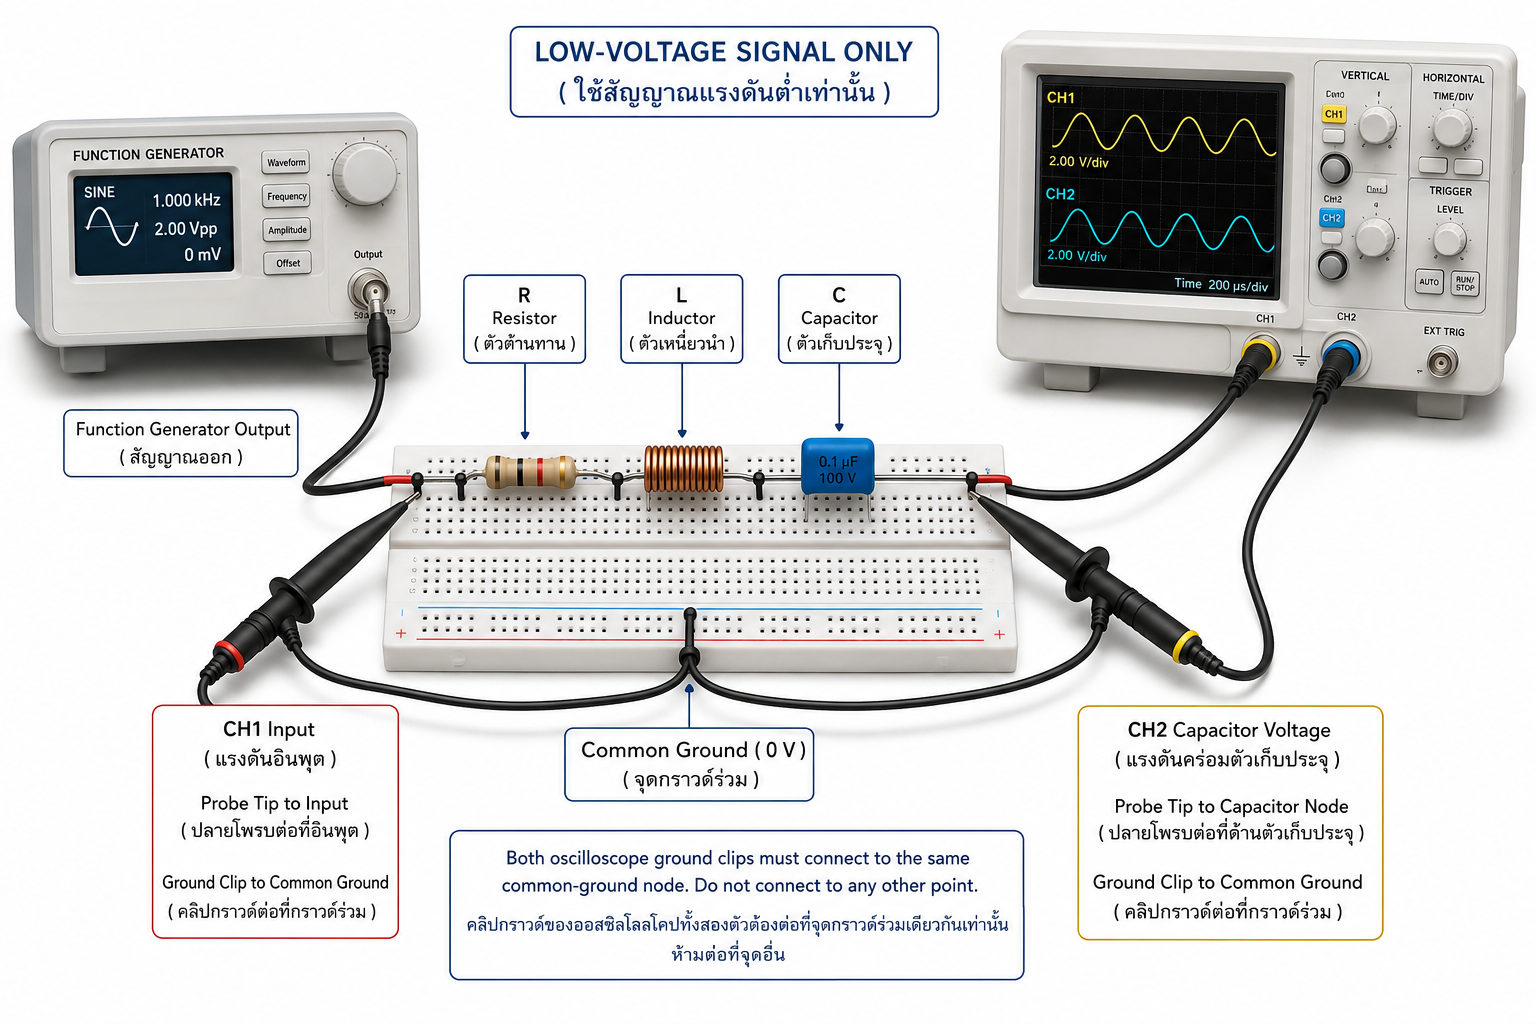
\includegraphics[width=0.8\textwidth]{images/chapter3/figure-10.png}
    \caption{ชุดทดลองวงจร RLC และจุดต่อ Oscilloscope}
\end{figure}

\subsubsection{9.4 ข้อควรระวังด้านความปลอดภัย}

\begin{enumerate}
    \item ใช้เฉพาะสัญญาณแรงดันต่ำจาก Function Generator ของห้องปฏิบัติการ \textbf{ห้ามต่อวงจรนี้เข้ากับไฟบ้านหรือแหล่งจ่ายที่ไม่แยกอย่างเหมาะสม}
    \item ปิดเอาต์พุต Function Generator ก่อนต่อหรือเปลี่ยนวงจร
    \item ตรวจสอบแผนผังรางของเบรดบอร์ดก่อนจ่ายสัญญาณ
    \item ตรวจสอบพิกัดกำลังของตัวต้านทานและพิกัดแรงดันของตัวเก็บประจุ
    \item Oscilloscope แบบตั้งโต๊ะทั่วไปมีกราวด์หัววัดเชื่อมกับสายดินป้องกัน จึงต้องต่อกราวด์ของทุกช่องที่โหนดกราวด์ร่วมเดียวกันเท่านั้น (Tektronix, n.d.)
    \item ห้ามคีบกราวด์หัววัดคร่อมองค์ประกอบหรือโหนดที่ไม่ใช่กราวด์ร่วม เพราะอาจทำให้โหนดนั้นถูกลัดวงจรลงดิน
    \item ห้ามเปลี่ยนการต่อวงจรขณะที่มีสัญญาณ
    \item หากอุปกรณ์ร้อน มีกลิ่นผิดปกติ หรือรูปคลื่นผิดปกติมาก ให้ปิดเอาต์พุตทันทีและแจ้งผู้สอน
    \item จัดสายให้เป็นระเบียบและหลีกเลี่ยงการสัมผัสตัวนำเปลือย
    \item การวัดวงจรที่ไม่อ้างอิงกราวด์หรือมีแรงดันสูงต้องใช้หัววัดและวิธีเฉพาะภายใต้การดูแลของผู้เชี่ยวชาญ ซึ่งไม่อยู่ในกิจกรรมนี้
\end{enumerate}

\subsubsection{9.5 ขั้นตอนการปฏิบัติ}

\paragraph{ตอนที่ 1: วัดพารามิเตอร์จริง}

\begin{enumerate}
    \item ปิด Function Generator และถอดแหล่งสัญญาณออกจากวงจร
    \item ใช้เครื่องมือวัดค่า $R$, $L$, $C$
    \item วัดความต้านทาน DC ของขดลวด $r_L$
    \item บันทึกค่าความต้านทานเอาต์พุตของ Function Generator จากคู่มือหรือค่าที่ผู้สอนกำหนด
    \item คำนวณ $R_{\text{eq}}$
\end{enumerate}

\paragraph{ตอนที่ 2: ต่อวงจร}

\begin{enumerate}
    \item ต่อ $R$, $L$, $C$ แบบอนุกรมบนเบรดบอร์ด
    \item กำหนดโหนดสุดท้ายของตัวเก็บประจุเป็นกราวด์ร่วม
    \item ต่อ Function Generator ที่อินพุตและกราวด์ร่วม
    \item ต่อ CH1 วัด $v_i(t)$ เทียบกราวด์ร่วม
    \item ต่อ CH2 วัด $v_o(t)=v_C(t)$ เทียบกราวด์ร่วม
    \item ให้ผู้สอนตรวจสอบก่อนเปิดสัญญาณ
\end{enumerate}

\paragraph{ตอนที่ 3: ตรวจสอบสัญญาณเบื้องต้น}

\begin{enumerate}
    \item ตั้งสัญญาณไซน์ประมาณ $1\ \text{V}_{pp}$, offset $0\ \text{V}$
    \item เริ่มที่ความถี่ต่ำกว่าความถี่ธรรมชาติอย่างน้อยหนึ่งลำดับขนาด เช่น $100\ \text{Hz}$
    \item ตรวจสอบว่า $v_o$ ใกล้ $v_i$ ที่ความถี่ต่ำ
    \item ตรวจสอบ Probe Ratio, Coupling และ Scale ของทั้งสองช่อง
    \item หากวงจรทำงานปกติ จึงเริ่มกวาดความถี่
\end{enumerate}

\paragraph{ตอนที่ 4: กวาดความถี่และบันทึกผล}

เลือกอย่างน้อย 10–15 จุดที่ครอบคลุมช่วงต่ำกว่า ใกล้ และสูงกว่าความถี่ธรรมชาติ ตัวอย่างช่วง $100$–$10{,}000\ \text{Hz}$ โดยเพิ่มจำนวนจุดใกล้บริเวณยอดเรโซแนนซ์

ในแต่ละความถี่

\begin{enumerate}
    \item รักษาแอมพลิจูดอินพุตให้คงที่
    \item วัด $V_{i,\text{pp}}$
    \item วัด $V_{o,\text{pp}}$
    \item วัด $\Delta t$ และระบุว่าเอาต์พุตนำหรือล้าหลัง
    \item คำนวณ $|G|$, $G_{\text{dB}}$ และ $\phi$
    \item บันทึกภาพหน้าจออย่างน้อยสามจุด: ความถี่ต่ำ ใกล้เรโซแนนซ์ และความถี่สูง
\end{enumerate}

\paragraph{ตอนที่ 5: สร้างแบบจำลองใน Simulink}

\begin{enumerate}
    \item สร้างแบบจำลอง \texttt{Transfer Fcn}
    \item แบบจำลองอุดมคติใช้ \texttt{[L*C R*C 1]}
    \item แบบจำลองเชิงปฏิบัติใช้ \texttt{[L*C Req*C 1]}
    \item ใช้ \texttt{Sine Wave} หรือสร้างการวิเคราะห์ความถี่ใน MATLAB ตามเครื่องมือที่มี
    \item จำลองที่ความถี่เดียวกับการทดลอง
    \item บันทึกแอมพลิจูดและเฟสของแบบจำลอง
    \item สร้างกราฟเปรียบเทียบข้อมูลทดลอง แบบจำลองอุดมคติ และแบบจำลองเชิงปฏิบัติ
\end{enumerate}

\subsubsection{9.6 ตารางบันทึกผล}

\paragraph{ตารางที่ 1 ค่าพารามิเตอร์}

\begin{table}[htbp]
    \centering
    \begin{tabular}{l r r l r}
        \hline
        \textbf{พารามิเตอร์} & \textbf{ค่าป้ายกำกับ} & \textbf{ค่าที่วัด} & \textbf{หน่วย} & \textbf{ความคลาดเคลื่อน (\%)} \\
        \hline
        $R$ &  &  & $\Omega$ &  \\
        $L$ &  &  & mH &  \\
        $r_L$ & ไม่ระบุ &  & $\Omega$ & — \\
        $C$ &  &  & $\mu$F &  \\
        $R_s$ &  &  & $\Omega$ &  \\
        $R_{\text{eq}}$ & — &  & $\Omega$ & — \\
        \hline
    \end{tabular}
\end{table}

\paragraph{ตารางที่ 2 ผลตอบสนองความถี่}

\begin{table}[htbp]
    \centering
    \begin{tabular}{r r r r r r r r l}
        \hline
        \textbf{ลำดับ} & \textbf{$f$ (Hz)} & \textbf{$V_{i,pp}$ (V)} & \textbf{$V_{o,pp}$ (V)} & \textbf{$|G|$} & \textbf{$G_{\text{dB}}$ (dB)} & \textbf{$\Delta t$ (s)} & \textbf{$\phi$ (deg)} & \textbf{หมายเหตุ} \\
        \hline
        1 &  &  &  &  &  &  &  &  \\
        2 &  &  &  &  &  &  &  &  \\
        3 &  &  &  &  &  &  &  &  \\
        4 &  &  &  &  &  &  &  &  \\
        5 &  &  &  &  &  &  &  &  \\
        6 &  &  &  &  &  &  &  &  \\
        7 &  &  &  &  &  &  &  &  \\
        8 &  &  &  &  &  &  &  &  \\
        9 &  &  &  &  &  &  &  &  \\
        10 &  &  &  &  &  &  &  &  \\
        11 &  &  &  &  &  &  &  &  \\
        12 &  &  &  &  &  &  &  &  \\
        \hline
    \end{tabular}
\end{table}

\paragraph{ตารางที่ 3 การเปรียบเทียบแบบจำลอง}

\begin{table}[htbp]
    \centering
    \begin{tabular}{r r r r r r}
        \hline
        \textbf{$f$ (Hz)} & \textbf{$|G|_{\text{meas}}$} & \textbf{$|G|_{\text{ideal}}$} & \textbf{$|G|_{\text{practical}}$} & \textbf{Error ideal (\%)} & \textbf{Error practical (\%)} \\
        \hline
         &  &  &  &  &  \\
         &  &  &  &  &  \\
         &  &  &  &  &  \\
        \hline
    \end{tabular}
\end{table}

\subsubsection{9.7 การคำนวณและวิเคราะห์ผล}

\begin{enumerate}
    \item ใช้ค่าที่วัดจริงสร้าง $G_{\text{ideal}}(s)$
    \item รวม $R_s$ และ $r_L$ เพื่อสร้าง $G_{\text{practical}}(s)$
    \item คำนวณ $\omega_n$, $f_n$ และ $\zeta$ ของทั้งสองแบบจำลอง
    \item คำนวณขนาดและเฟสตามความถี่ที่ทดลอง
    \item สร้างกราฟแกนความถี่ลอการิทึม
    \item เปรียบเทียบตำแหน่งและขนาดยอดเรโซแนนซ์
    \item คำนวณความคลาดเคลื่อนแบบจุดต่อจุด
    \item อภิปรายว่าพารามิเตอร์ใดมีผลต่อความแตกต่างมากที่สุด
\end{enumerate}

ตัวอย่างความคลาดเคลื่อนขนาดอัตราขยาย

\[
\%\text{Error}_k
=
\left|
\frac{|G|_{\text{meas},k}-|G|_{\text{model},k}}
{|G|_{\text{model},k}}
\right|\times100
\]

เมื่อค่าตัวหารใกล้ศูนย์ ควรหลีกเลี่ยงการตีความเปอร์เซ็นต์เพียงอย่างเดียวและรายงานความคลาดเคลื่อนสัมบูรณ์ร่วมด้วย

\subsubsection{9.8 การเปรียบเทียบผลจริงกับทฤษฎีหรือแบบจำลอง}

รายงานควรประกอบด้วย

\begin{itemize}
    \item ตารางพารามิเตอร์จริง
    \item Transfer Function อุดมคติและเชิงปฏิบัติ
    \item กราฟขนาดและเฟสสามชุด
    \item ภาพหน้าจอ Oscilloscope
    \item ค่าเรโซแนนซ์จากทฤษฎี จำลอง และทดลอง
    \item การอภิปรายโหลดจากเครื่องมือวัด
    \item การอภิปรายค่าคลาดเคลื่อนของอุปกรณ์
    \item ข้อเสนอปรับปรุงแบบจำลองหรือวิธีทดลอง
\end{itemize}

\textbf{ห้ามสร้างหรือเติมค่าที่ไม่ได้วัดจริง} หากข้อมูลบางจุดใช้ไม่ได้ ให้ระบุสาเหตุและทำซ้ำการวัด

\subsubsection{9.9 คำถามหลังการทดลอง}

\begin{enumerate}
    \item เหตุใด $R_{\text{eq}}$ จึงทำให้ยอดเรโซแนนซ์ลดลง
    \item หากเพิ่ม $R$ เป็นสองเท่า ค่า $\omega_n$ และ $\zeta$ เปลี่ยนอย่างไร
    \item เหตุใดแรงดันคร่อมตัวเก็บประจุอาจสูงกว่าแรงดันอินพุตใกล้เรโซแนนซ์
    \item ความต้านทานอินพุตและความจุของหัววัดมีผลต่อวงจรอย่างไร
    \item หากวัดเอาต์พุตคร่อมตัวต้านทาน ฟังก์ชันถ่ายโอนจะเปลี่ยนเป็นแบบใด
    \item เพราะเหตุใดกราฟเฟสจากการวัด $\Delta t$ จึงอ่านยากเมื่อความถี่สูง
    \item แบบจำลองอุดมคติหรือเชิงปฏิบัติสอดคล้องกับผลทดลองมากกว่า เพราะเหตุใด
    \item หากผลจำลองไม่ตรงสมการคำนวณ ควรตรวจสอบรายการใดก่อน
\end{enumerate}

\subsubsection{9.10 เกณฑ์การประเมินกิจกรรมปฏิบัติการ}

\begin{table}[htbp]
    \centering
    \begin{tabular}{l r l l l}
        \hline
        \textbf{ด้านประเมิน} & \textbf{น้ำหนัก} & \textbf{ดีเยี่ยม} & \textbf{ผ่านเกณฑ์} & \textbf{ต้องปรับปรุง} \\
        \hline
        ความถูกต้องของการต่อวงจร & 15\% & ต่อถูกและตรวจสอบเป็นระบบ & มีข้อผิดพลาดเล็กน้อย แก้ไขได้ & ต่อผิดหรือไม่ตรวจสอบ \\
        ความปลอดภัยและการใช้เครื่องมือ & 15\% & ปฏิบัติตามข้อกำหนดครบ & มีการเตือนเล็กน้อย & เสี่ยงต่ออุปกรณ์หรือผู้ใช้ \\
        การวัดและบันทึกข้อมูล & 20\% & ข้อมูลครบ หน่วยและเงื่อนไขชัด & ขาดบางจุดแต่ยังวิเคราะห์ได้ & ข้อมูลไม่พอหรือไม่น่าเชื่อถือ \\
        การคำนวณ Transfer Function & 15\% & สมการและพารามิเตอร์ถูกต้อง & ผิดเล็กน้อย & ไม่สามารถเชื่อมสมการกับวงจร \\
        แบบจำลอง MATLAB/Simulink & 15\% & สร้างและตรวจสอบได้ครบ & แบบจำลองทำงานแต่ขาดการตรวจสอบ & แบบจำลองไม่ทำงาน \\
        การเปรียบเทียบและอภิปราย & 15\% & อธิบายความคลาดเคลื่อนด้วยเหตุผล & เปรียบเทียบได้ระดับพื้นฐาน & สรุปโดยไม่มีหลักฐาน \\
        รายงานและการสื่อสาร & 5\% & ชัดเจน เป็นระบบ อ้างรูปและตาราง & อ่านเข้าใจได้ & ไม่เป็นระบบ \\
        \hline
    \end{tabular}
\end{table}

\par\noindent\rule{\textwidth}{0.4pt}\par

\subsection{10. ความเข้าใจผิดที่พบบ่อย}

\begin{table}[htbp]
    \centering
    \begin{tabular}{l l}
        \hline
        \textbf{ความเข้าใจคลาดเคลื่อน} & \textbf{แนวคิดที่ถูกต้อง} \\
        \hline
        ฟังก์ชันถ่ายโอนคืออัตราส่วน $y(t)/u(t)$ & ต้องเป็นอัตราส่วน $Y(s)/U(s)$ ในโดเมนลาปลาซ ภายใต้เงื่อนไขที่กำหนด \\
        ค่าเริ่มต้นไม่เกี่ยวกับ Transfer Function & การนิยามแบบมาตรฐานใช้อัตราส่วนภายใต้ค่าเริ่มต้นเป็นศูนย์ \\
        วงจรหรือระบบหนึ่งมี Transfer Function เพียงชุดเดียว & ฟังก์ชันถ่ายโอนขึ้นกับการเลือกอินพุตและเอาต์พุต \\
        จำนวนองค์ประกอบสะสมพลังงานเท่ากับอันดับเสมอ & อาจมีข้อจำกัดหรือการพึ่งพากัน ทำให้อันดับลดลง \\
        ใช้ตัวหารแรงดันกับอิมพีแดนซ์ได้โดยไม่สนใจค่าเริ่มต้น & รูปอิมพีแดนซ์ $sL$ และ $1/(sC)$ แบบง่ายสอดคล้องกับค่าเริ่มต้นเป็นศูนย์ \\
        โพลคือค่าพารามิเตอร์ทางกายภาพโดยตรง & โพลเป็นรากของสมการลักษณะเฉพาะและเกิดจากการรวมพารามิเตอร์ \\
        State-Space ที่แปลงจาก Transfer Function มีเพียงรูปเดียว & realization ไม่เป็นเอกลักษณ์ แม้ให้พฤติกรรมอินพุต–เอาต์พุตเดียวกัน \\
        ผล Simulink คือความจริงของระบบ & ผลจำลองถูกต้องตามแบบจำลองและค่าพารามิเตอร์ที่ใส่เท่านั้น \\
        กราวด์หัววัด Oscilloscope ต่อที่ใดก็ได้ & สำหรับเครื่องตั้งโต๊ะทั่วไป กราวด์หัววัดมักผูกกับสายดิน ต้องต่อที่โหนดกราวด์ร่วม \\
        เพิ่มรายละเอียดมากทำให้แบบจำลองดีกว่าเสมอ & แบบจำลองควรละเอียดพอสำหรับวัตถุประสงค์ แต่ไม่ซับซ้อนเกินจำเป็น \\
        \hline
    \end{tabular}
\end{table}

\par\noindent\rule{\textwidth}{0.4pt}\par

\subsection{11. การประยุกต์ใช้ในงานจริง}

\subsubsection{11.1 ระบบกันสะเทือนและเครื่องจักร}

แบบจำลองมวล–สปริง–ตัวหน่วงใช้ประมาณการสั่นสะเทือนของยานพาหนะ เครื่องจักร โครงสร้าง และระบบแยกแรงสั่น การวิเคราะห์ช่วยเลือกความแข็งและการหน่วงเพื่อหลีกเลี่ยงเรโซแนนซ์หรือจำกัดการสั่น

\subsubsection{11.2 วงจรกรองและระบบวัด}

RC, RL และ RLC ใช้เป็นพื้นฐานของวงจรกรอง สัญญาณปรับสภาพ และอินเทอร์เฟซเซนเซอร์ Transfer Function ช่วยประเมินแบนด์วิดท์ การลดทอน และเฟสก่อนสร้างวงจรจริง

\subsubsection{11.3 ระบบขับเคลื่อนด้วยมอเตอร์}

แบบจำลองมอเตอร์ DC เชื่อมแรงดัน กระแส แรงบิด และความเร็ว ใช้เลือกตัวควบคุมความเร็ว ตำแหน่ง หรือแรงบิด และใช้ประเมินผลกระทบจากโหลดรบกวน

\subsubsection{11.4 ระบบควบคุมกระบวนการ}

แม้กระบวนการจริงอาจซับซ้อน แต่แบบจำลองอันดับหนึ่งหรืออันดับสองสามารถใช้ประมาณพฤติกรรมรอบจุดทำงาน เช่น อุณหภูมิ ระดับของเหลว และอัตราการไหล เพื่อออกแบบตัวควบคุมเบื้องต้น

\subsubsection{11.5 Digital Twin และ Model-Based Design}

แนวคิดการสร้างแบบจำลองเป็นฐานของการออกแบบโดยใช้แบบจำลอง การทดสอบแบบจำลองก่อนฮาร์ดแวร์ และ Digital Twin อย่างไรก็ตาม แบบจำลองต้องผ่านการปรับพารามิเตอร์และตรวจสอบกับข้อมูลจริงอย่างต่อเนื่อง

\par\noindent\rule{\textwidth}{0.4pt}\par

\subsection{12. สรุปท้ายบท}

\begin{enumerate}
    \item แบบจำลองทางคณิตศาสตร์เป็นตัวแทนของพฤติกรรมระบบภายใต้สมมติฐานและขอบเขตที่ชัดเจน
    \item กระบวนการสำคัญคือกำหนดระบบ เลือกอินพุต–เอาต์พุต ใช้กฎทางฟิสิกส์ สร้างสมการเชิงอนุพันธ์ แปลงลาปลาซ และตรวจสอบแบบจำลอง
    \item ฟังก์ชันถ่ายโอนของระบบ LTI นิยามเป็น
\end{enumerate}

\[
G(s)=\frac{Y(s)}{U(s)}
\]

ภายใต้ค่าเริ่มต้นเป็นศูนย์

\begin{enumerate}
    \item โพล ซีโร และอัตราขยายให้ข้อมูลเชิงโครงสร้างของพฤติกรรมอินพุต–เอาต์พุต
    \item ระบบมวล–สปริง–ตัวหน่วงมี
\end{enumerate}

\[
\frac{X(s)}{F(s)}=\frac{1}{ms^2+cs+k}
\]

\begin{enumerate}
    \item วงจร RC ผ่านต่ำมี
\end{enumerate}

\[
\frac{V_C(s)}{V_i(s)}=\frac{1}{RCs+1}
\]

\begin{enumerate}
    \item วงจร RLC อนุกรมที่วัดคร่อม $C$ มี
\end{enumerate}

\[
\frac{V_C(s)}{V_i(s)}=\frac{1}{LCs^2+RCs+1}
\]

\begin{enumerate}
    \item มอเตอร์ DC ต้องเชื่อมสมการวงจรอาร์เมเจอร์กับสมการกล และมี Back EMF เป็นป้อนกลับภายใน
    \item State-Space แสดงพลวัตภายใน และ realization ของ Transfer Function ไม่เป็นเอกลักษณ์
    \item MATLAB/Simulink เป็นเครื่องมือช่วยคำนวณและจำลอง แต่ไม่แทนการตรวจสอบสมมติฐาน หน่วย และผลทดลอง
    \item ความต่างระหว่างผลทดลองกับแบบจำลองสามารถใช้ระบุพารามิเตอร์แฝงและปรับปรุงแบบจำลองให้เหมาะกับวัตถุประสงค์
\end{enumerate}

\par\noindent\rule{\textwidth}{0.4pt}\par

\subsection{13. คำถามทบทวน}

\begin{enumerate}
    \item แบบจำลองทางคณิตศาสตร์มีบทบาทอย่างไรในการออกแบบระบบควบคุม
    \item อธิบายเงื่อนไขสำคัญของการนิยาม Transfer Function
    \item เพราะเหตุใดต้องกำหนดอินพุตและเอาต์พุตก่อนสร้างแบบจำลอง
    \item อธิบายความหมายของโพล ซีโร และอัตราขยาย
    \item เปรียบเทียบระบบอันดับหนึ่งกับระบบอันดับสอง
    \item เขียนขั้นตอนการสร้างแบบจำลองมวล–สปริง–ตัวหน่วง
    \item วงจร RL เดียวกันให้พฤติกรรมผ่านต่ำหรือผ่านสูงได้อย่างไร
    \item Back EMF ของมอเตอร์ DC มีผลต่อความเร็วอย่างไร
    \item Transfer Function และ State-Space ต่างกันในด้านข้อมูลที่แสดงอย่างไร
    \item ระบุสาเหตุอย่างน้อยสี่ประการที่ทำให้ผลทดลองต่างจากผลจำลอง
\end{enumerate}

\par\noindent\rule{\textwidth}{0.4pt}\par

\subsection{14. แบบฝึกหัดท้ายบท}

\subsubsection{14.1 ระดับพื้นฐาน}

\textbf{ข้อ 1} อธิบายความหมายของแบบจำลองทางคณิตศาสตร์ และยกตัวอย่างสมมติฐานหนึ่งข้อที่ใช้ในการสร้างแบบจำลองระบบจริง

\textbf{ข้อ 2} กำหนดสมการ

\[
3\dot{y}(t)+6y(t)=2u(t)
\]

จงหา $G(s)=Y(s)/U(s)$ ภายใต้ค่าเริ่มต้นเป็นศูนย์ พร้อมระบุอันดับ โพล และอัตราขยาย DC

\textbf{ข้อ 3} วงจร RC ผ่านต่ำมี $R=10\ \text{k}\Omega$ และ $C=10\ \mu\text{F}$ จงหาค่าคงตัวเวลาและความถี่ตัด

\textbf{ข้อ 4} จงอธิบายเหตุผลที่ Transfer Function มาตรฐานต้องกำหนดค่าเริ่มต้นเป็นศูนย์

\textbf{ข้อ 5} ให้

\[
G(s)=\frac{5}{s^2+4s+5}
\]

จงระบุเมทริกซ์ $A,B,C,D$ ในรูป controllable canonical form หนึ่งรูป

\subsubsection{14.2 ระดับวิเคราะห์}

\textbf{ข้อ 6} ระบบมวล–สปริง–ตัวหน่วงมี $m=4\ \text{kg}$, $c=8\ \text{N·s/m}$ และ $k=16\ \text{N/m}$ อินพุตเป็นแรง เอาต์พุตเป็นการกระจัด จงสร้างสมการเชิงอนุพันธ์ หา Transfer Function, $\omega_n$ และ $\zeta$

\textbf{ข้อ 7} วงจร RL อนุกรมมี $R=20\ \Omega$ และ $L=0.2\ \text{H}$\\ก. หา Transfer Function เมื่อวัดเอาต์พุตคร่อม $R$\\ข. หา Transfer Function เมื่อวัดเอาต์พุตคร่อม $L$\\ค. อธิบายพฤติกรรมที่ความถี่ต่ำและสูง

\textbf{ข้อ 8} วงจร RLC อนุกรมมี $R=50\ \Omega$, $L=20\ \text{mH}$, $C=5\ \mu\text{F}$ วัดเอาต์พุตคร่อม $C$ จงหา Transfer Function, $\omega_n$, $f_n$ และ $\zeta$

\textbf{ข้อ 9} วงจร Op-Amp กลับเฟสมี $R_{in}=10\ \text{k}\Omega$, $R_f=100\ \text{k}\Omega$ และ $C_f=10\ \text{nF}$ ต่อ $C_f$ ขนานกับ $R_f$ จงหา Transfer Function อัตราขยายความถี่ต่ำ และความถี่โพล

\textbf{ข้อ 10} มอเตอร์ DC มี

\[
J=0.02,\quad b=0.05,\quad
R_a=2,\quad L_a=0.1,\quad
K_t=K_e=0.2
\]

ใช้หน่วย SI จงหา $\Omega(s)/V_a(s)$ เมื่อ $T_L=0$ และหาอัตราขยาย DC

\subsubsection{14.3 ระดับประยุกต์ใช้}

\textbf{ข้อ 11} ในการทดลอง RLC ใช้ $R=100\ \Omega$, $L=10\ \text{mH}$, $C=1\ \mu\text{F}$ แต่ Function Generator มี $R_s=50\ \Omega$ และตัวเหนี่ยวนำมี $r_L=20\ \Omega$\\ก. สร้างแบบจำลองเชิงปฏิบัติ\\ข. เปรียบเทียบ $\zeta$ กับแบบจำลองอุดมคติ\\ค. อธิบายผลต่อยอดเรโซแนนซ์

\textbf{ข้อ 12} นักศึกษาสร้างแบบจำลอง Simulink ของวงจร RLC โดยใส่ Denominator เป็น \texttt{[1 R*C L*C]} และได้กราฟไม่ตรงกับการคำนวณ จงวิเคราะห์ข้อผิดพลาด เขียนเวกเตอร์ที่ถูกต้อง และเสนอรายการตรวจสอบอีกอย่างน้อยสามข้อ

\textbf{ข้อ 13} ผลทดลองของวงจร RLC มีความถี่ยอดอัตราขยายต่ำกว่าแบบจำลองอุดมคติ และยอดต่ำกว่าอย่างชัดเจน จงเสนอสมมติฐานสาเหตุอย่างน้อยสี่ข้อ ระบุวิธีตรวจสอบแต่ละข้อ และอธิบายว่าจะปรับแบบจำลองอย่างไร

\newpage

\subsection{15. แนวคำตอบและเฉลยแบบฝึกหัด}

\begin{quote}
\textbf{ส่วนสำหรับผู้สอน:} ควรแยกส่วนนี้ออกจากเอกสารนักศึกษาเมื่อใช้เป็นงานมอบหมายหรือการประเมิน
\end{quote}

\subsubsection{15.1 เฉลยระดับพื้นฐาน}

\paragraph{เฉลยข้อ 1}

\textbf{แนวคิดที่ใช้:} แบบจำลองทางคณิตศาสตร์เป็นการแทนความสัมพันธ์ของตัวแปรและพลวัตของระบบจริงด้วยสมการ เพื่อใช้วิเคราะห์ ทำนาย จำลอง หรือออกแบบระบบควบคุม

ตัวอย่างสมมติฐาน ได้แก่

\begin{itemize}
    \item สปริงทำงานในช่วงเชิงเส้น จึงใช้ $F_s=kx$
    \item แรงเสียดทานเป็นแบบหนืด จึงใช้ $F_d=c\dot{x}$
    \item ค่า $R$, $L$, $C$ คงที่
    \item Op-Amp ทำงานในช่วงไม่อิ่มตัว
    \item มอเตอร์ทำงานรอบจุดที่ค่าคงตัวแรงบิดและ Back EMF คงที่
\end{itemize}

\textbf{การแปลความหมาย:} แบบจำลองไม่ใช่สำเนาของระบบจริง แต่เป็นตัวแทนที่มีความละเอียดเหมาะกับวัตถุประสงค์ สมมติฐานจึงต้องระบุและตรวจสอบ

\paragraph{เฉลยข้อ 2}

กำหนด

\[
3\dot{y}(t)+6y(t)=2u(t)
\]

แปลงลาปลาซเมื่อ $y(0)=0$

\[
3sY(s)+6Y(s)=2U(s)
\]

จัดรูป

\[
(3s+6)Y(s)=2U(s)
\]

ดังนั้น

\[
\boxed{
G(s)=\frac{Y(s)}{U(s)}
=\frac{2}{3s+6}
=\frac{2/3}{s+2}
}
\]

\begin{itemize}
    \item อันดับระบบ: 1
    \item โพล: $s=-2$
    \item ซีโรจำกัด: ไม่มี
    \item อัตราขยาย DC:
\end{itemize}

\[
G(0)=\frac{2}{6}=\boxed{\frac{1}{3}}
\]

\textbf{ข้อผิดพลาดที่พบบ่อย:} ลืมว่าตัวคูณ 3 ต้องคงอยู่ทั้งก่อนและหลังแปลงลาปลาซ

\paragraph{เฉลยข้อ 3}

\[
R=10\ \text{k}\Omega=10{,}000\ \Omega
\]

\[
C=10\ \mu\text{F}=10\times10^{-6}\ \text{F}
\]

ค่าคงตัวเวลา

\[
\tau=RC
=(10{,}000)(10\times10^{-6})
=\boxed{0.1\ \text{s}}
\]

ความถี่ตัดเชิงมุม

\[
\omega_c=\frac{1}{RC}=10\ \text{rad/s}
\]

ความถี่ตัดหน่วยเฮิรตซ์

\[
f_c=\frac{1}{2\pi RC}
=\frac{1}{2\pi(0.1)}
\approx\boxed{1.59\ \text{Hz}}
\]

\paragraph{เฉลยข้อ 4}

เมื่อแปลงอนุพันธ์ด้วยลาปลาซ จะเกิดพจน์ค่าเริ่มต้น เช่น

\[
\mathcal{L}\{\dot{y}\}=sY(s)-y(0)
\]

หาก $y(0)\neq0$ ความสัมพันธ์ $Y(s)$ จะมีทั้งผลจากอินพุตและผลจากพลังงานเริ่มต้น จึงไม่สามารถนิยาม $Y(s)/U(s)$ เป็นคุณสมบัติของระบบเพียงอย่างเดียวได้อย่างตรงไปตรงมา การกำหนดค่าเริ่มต้นเป็นศูนย์ทำให้

\[
Y(s)=G(s)U(s)
\]

และ $G(s)$ ขึ้นกับพารามิเตอร์ระบบ ไม่ขึ้นกับอินพุตเฉพาะครั้งหรือสถานะเริ่มต้น

\paragraph{เฉลยข้อ 5}

ให้

\[
G(s)=\frac{5}{s^2+4s+5}
\]

เปรียบเทียบกับ

\[
G(s)=\frac{b_1s+b_0}{s^2+a_1s+a_0}
\]

ได้

\[
a_1=4,\quad a_0=5,\quad b_1=0,\quad b_0=5
\]

รูป controllable canonical form หนึ่งรูปคือ

\[
\boxed{
A=
\begin{bmatrix}
0 & 1\\
-5 & -4
\end{bmatrix},
\quad
B=
\begin{bmatrix}
0\\
1
\end{bmatrix},
\quad
C=
\begin{bmatrix}
5 & 0
\end{bmatrix},
\quad
D=0
}
\]

ตรวจสอบด้วย $G(s)=C(sI-A)^{-1}B+D$ จะได้ฟังก์ชันถ่ายโอนเดิม

\subsubsection{15.2 เฉลยระดับวิเคราะห์}

\paragraph{เฉลยข้อ 6}

กำหนด

\[
m=4\ \text{kg},\quad
c=8\ \text{N·s/m},\quad
k=16\ \text{N/m}
\]

สมการแรง

\[
F(t)-c\dot{x}(t)-kx(t)=m\ddot{x}(t)
\]

จัดรูป

\[
\boxed{
4\ddot{x}(t)+8\dot{x}(t)+16x(t)=F(t)
}
\]

แปลงลาปลาซภายใต้ค่าเริ่มต้นเป็นศูนย์

\[
(4s^2+8s+16)X(s)=F(s)
\]

ดังนั้น

\[
\boxed{
\frac{X(s)}{F(s)}
=
\frac{1}{4s^2+8s+16}
}
\]

ความถี่ธรรมชาติ

\[
\omega_n=\sqrt{\frac{k}{m}}
=\sqrt{\frac{16}{4}}
=\boxed{2\ \text{rad/s}}
\]

อัตราส่วนการหน่วง

\[
\zeta=\frac{c}{2\sqrt{mk}}
=
\frac{8}{2\sqrt{(4)(16)}}
=
\frac{8}{16}
=\boxed{0.5}
\]

ระบบเป็น underdamped เพราะ $0<\zeta<1$

\paragraph{เฉลยข้อ 7}

กำหนด $R=20\ \Omega$, $L=0.2\ \text{H}$

\textbf{ก. เอาต์พุตคร่อม ZZPROTECTED0ZZ}

\[
\frac{V_R(s)}{V_i(s)}
=
\frac{R}{Ls+R}
=
\frac{20}{0.2s+20}
\]

หารด้วย $0.2$

\[
\boxed{
G_R(s)=\frac{100}{s+100}
}
\]

\textbf{ข. เอาต์พุตคร่อม ZZPROTECTED0ZZ}

\[
\frac{V_L(s)}{V_i(s)}
=
\frac{Ls}{Ls+R}
=
\frac{0.2s}{0.2s+20}
\]

\[
\boxed{
G_L(s)=\frac{s}{s+100}
}
\]

\textbf{ค. พฤติกรรม}

\begin{itemize}
    \item เมื่อ $\omega\rightarrow0$: $G_R(j\omega)\rightarrow1$, $G_L(j\omega)\rightarrow0$
    \item เมื่อ $\omega\rightarrow\infty$: $G_R(j\omega)\rightarrow0$, $G_L(j\omega)\rightarrow1$
\end{itemize}

ดังนั้นเอาต์พุตคร่อม $R$ เป็นผ่านต่ำ และเอาต์พุตคร่อม $L$ เป็นผ่านสูง

\paragraph{เฉลยข้อ 8}

กำหนด

\[
R=50\ \Omega,\quad
L=20\ \text{mH}=0.02\ \text{H}
\]

\[
C=5\ \mu\text{F}=5\times10^{-6}\ \text{F}
\]

คำนวณ

\[
LC=(0.02)(5\times10^{-6})=1\times10^{-7}
\]

\[
RC=(50)(5\times10^{-6})=2.5\times10^{-4}
\]

Transfer Function

\[
\boxed{
G(s)=
\frac{1}{10^{-7}s^2+2.5\times10^{-4}s+1}
}
\]

หรือ

\[
\boxed{
G(s)=
\frac{10^7}{s^2+2500s+10^7}
}
\]

ความถี่ธรรมชาติ

\[
\omega_n=\frac{1}{\sqrt{LC}}
=\frac{1}{\sqrt{10^{-7}}}
\approx\boxed{3162.28\ \text{rad/s}}
\]

\[
f_n=\frac{\omega_n}{2\pi}
\approx\boxed{503.29\ \text{Hz}}
\]

อัตราส่วนการหน่วง

\[
\zeta=
\frac{R}{2}\sqrt{\frac{C}{L}}
=
25\sqrt{\frac{5\times10^{-6}}{0.02}}
\]

\[
\zeta
=25\sqrt{2.5\times10^{-4}}
\approx\boxed{0.395}
\]

ระบบเป็น underdamped และมีแนวโน้มเกิดยอดเรโซแนนซ์

\paragraph{เฉลยข้อ 9}

กำหนด

\[
R_{in}=10\ \text{k}\Omega,\quad
R_f=100\ \text{k}\Omega,\quad
C_f=10\ \text{nF}
\]

Transfer Function

\[
G(s)=
-\frac{R_f/R_{in}}{1+sR_fC_f}
\]

อัตราขยายความถี่ต่ำ

\[
-\frac{R_f}{R_{in}}
=-\frac{100}{10}
=\boxed{-10}
\]

ค่าคงตัวเวลา

\[
R_fC_f=(100\times10^3)(10\times10^{-9})
=10^{-3}\ \text{s}
\]

ดังนั้น

\[
\boxed{
G(s)=\frac{-10}{1+0.001s}
}
\]

ความถี่โพล

\[
\omega_p=\frac{1}{R_fC_f}
=\boxed{1000\ \text{rad/s}}
\]

\[
f_p=\frac{1000}{2\pi}
\approx\boxed{159.15\ \text{Hz}}
\]

\paragraph{เฉลยข้อ 10}

สมการทั่วไป

\[
\frac{\Omega(s)}{V_a(s)}
=
\frac{K_t}
{L_aJs^2+(L_ab+R_aJ)s+(R_ab+K_tK_e)}
\]

แทนค่า

\[
L_aJ=(0.1)(0.02)=0.002
\]

\[
L_ab+R_aJ=(0.1)(0.05)+(2)(0.02)
=0.005+0.04=0.045
\]

\[
R_ab+K_tK_e=(2)(0.05)+(0.2)(0.2)
=0.1+0.04=0.14
\]

จึงได้

\[
\boxed{
\frac{\Omega(s)}{V_a(s)}
=
\frac{0.2}{0.002s^2+0.045s+0.14}
}
\]

หารทั้งเศษและส่วนด้วย $0.002$

\[
\boxed{
\frac{\Omega(s)}{V_a(s)}
=
\frac{100}{s^2+22.5s+70}
}
\]

อัตราขยาย DC

\[
G(0)=\frac{0.2}{0.14}
\approx\boxed{1.429\ \frac{\text{rad/s}}{\text{V}}}
\]

\subsubsection{15.3 เฉลยระดับประยุกต์ใช้}

\paragraph{เฉลยข้อ 11}

กำหนด

\[
R=100\ \Omega,\quad
R_s=50\ \Omega,\quad
r_L=20\ \Omega
\]

ดังนั้น

\[
R_{\text{eq}}=100+50+20=170\ \Omega
\]

\textbf{ก. แบบจำลองเชิงปฏิบัติ}

เมื่อ $L=10^{-2}\ \text{H}$ และ $C=10^{-6}\ \text{F}$

\[
LC=10^{-8}
\]

\[
R_{\text{eq}}C=(170)(10^{-6})=1.7\times10^{-4}
\]

จึงได้

\[
\boxed{
G_p(s)
=
\frac{1}{10^{-8}s^2+1.7\times10^{-4}s+1}
}
\]

\textbf{ข. เปรียบเทียบอัตราส่วนการหน่วง}

แบบอุดมคติที่ใช้ $R=100\ \Omega$

\[
\zeta_{\text{ideal}}
=
\frac{100}{2}\sqrt{\frac{10^{-6}}{10^{-2}}}
=0.5
\]

แบบเชิงปฏิบัติ

\[
\zeta_{\text{practical}}
=
\frac{170}{2}\sqrt{\frac{10^{-6}}{10^{-2}}}
=85(0.01)
=\boxed{0.85}
\]

\textbf{ค. ผลต่อยอดเรโซแนนซ์}

การเพิ่มความต้านทานทำให้การหน่วงสูงขึ้น จาก $\zeta=0.5$ เป็น $0.85$ สำหรับรูปผ่านต่ำอันดับสอง เมื่อ $\zeta\geq1/\sqrt{2}$ จะไม่มียอดเรโซแนนซ์ของขนาดอัตราขยายแบบเด่นชัด ดังนั้นผลจริงควรมียอดต่ำกว่าหรือไม่มีจุดยอดชัดเมื่อเทียบกับแบบอุดมคติ

\paragraph{เฉลยข้อ 12}

สมการส่วนของวงจรคือ

\[
LCs^2+RCs+1
\]

เวกเตอร์สัมประสิทธิ์ต้องเรียงจากกำลังสูงไปต่ำ คือ

\[
\boxed{[L*C,\ R*C,\ 1]}
\]

สำหรับค่าตัวอย่าง $L=10\ \text{mH}$, $C=1\ \mu\text{F}$, $R=100\ \Omega$

\[
\boxed{[1e-8,\ 1e-4,\ 1]}
\]

การใส่ \texttt{[1 R*C L*C]} แทนพหุนาม

\[
s^2+RCs+LC
\]

ซึ่งไม่ใช่สมการเดิมและมีหน่วยไม่สอดคล้องกัน

รายการตรวจสอบเพิ่มเติม

\begin{enumerate}
    \item แปลง mH และ $\mu$F เป็น H และ F แล้วหรือไม่
    \item Numerator ถูกต้องหรือไม่
    \item Stop Time ยาวพอหรือไม่
    \item Solver และ Max Step Size เหมาะกับไดนามิกเร็วหรือไม่
    \item ค่าเริ่มต้นของ Integrator ตรงกันหรือไม่
    \item เลือกเอาต์พุตคร่อมองค์ประกอบเดียวกับแบบจำลองหรือไม่
    \item สัญญาณป้อนเข้ามีแอมพลิจูดและหน่วยตรงกันหรือไม่
\end{enumerate}

\paragraph{เฉลยข้อ 13}

ตัวอย่างการวิเคราะห์อย่างเป็นระบบ

\begin{table}[htbp]
    \centering
    \begin{tabular}{l l l}
        \hline
        \textbf{สมมติฐานสาเหตุ} & \textbf{วิธีตรวจสอบ} & \textbf{การปรับแบบจำลอง} \\
        \hline
        มี $R_s$ และ $r_L$ ที่ละเลย & อ่านสเปก Function Generator และวัดความต้านทานขดลวด & ใช้ $R_{\text{eq}}=R+R_s+r_L$ \\
        ค่า $L$ หรือ $C$ จริงต่างจากป้าย & วัดด้วย LCR Meter & แทนค่าที่วัดจริง \\
        ตัวเก็บประจุมี ESR & ใช้เครื่องมือวัด ESR หรือเปรียบเทียบหลายชนิด & เพิ่ม $R_{\text{ESR}}$ ในแบบจำลอง \\
        หัววัดและ Oscilloscope โหลดวงจร & ตรวจค่า input resistance/capacitance และเปลี่ยน probe ratio & เพิ่มอิมพีแดนซ์หัววัดขนานกับจุดวัด \\
        การต่อบนเบรดบอร์ดมีพาราซิติก & ลดความยาวสาย เปลี่ยนการจัดวาง และทำซ้ำ & เพิ่ม $L_p$ หรือ $C_p$ เมื่อจำเป็น \\
        แอมพลิจูดแหล่งกำเนิดเปลี่ยนตามโหลด & วัด $V_i$ ทุกความถี่แทนการสมมติคงที่ & ใช้ $V_o/V_i$ จากค่าที่วัดจริง \\
        ความละเอียดการวัดเฟสหรือความถี่ไม่พอ & เพิ่มจุดใกล้ยอดและใช้ cursor/fit & ปรับวิธีเก็บข้อมูล ไม่จำเป็นต้องเพิ่มไดนามิก \\
        ตัวเหนี่ยวนำไม่เชิงเส้นหรือมี core loss & เปลี่ยนแอมพลิจูดและสังเกตว่าค่าตอบสนองเปลี่ยนหรือไม่ & ใช้แบบจำลองขึ้นกับแอมพลิจูดหรือเพิ่ม loss term \\
        \hline
    \end{tabular}
\end{table}

ความถี่ยอดที่ต่ำลงมักสัมพันธ์กับค่า $LC$ จริงสูงกว่าที่สมมติ หรือมีพาราซิติกที่เพิ่มค่าการสะสมพลังงาน ส่วนยอดที่ต่ำลงสัมพันธ์กับความต้านทานรวมและการสูญเสียสูงขึ้น ควรวัดพารามิเตอร์ก่อนสรุปสาเหตุ

\par\noindent\rule{\textwidth}{0.4pt}\par

\subsection{16. ข้อเสนอแนะสำหรับผู้สอน}

\subsubsection{16.1 แผนการสอน 6 ชั่วโมง}

\begin{table}[htbp]
    \centering
    \begin{tabular}{l l l l}
        \hline
        \textbf{ช่วงเวลา} & \textbf{เนื้อหาและกิจกรรม} & \textbf{วิธีสอน} & \textbf{หลักฐานระหว่างเรียน} \\
        \hline
        ชั่วโมงที่ 1 & ความหมายแบบจำลอง ขั้นตอนสร้างแบบจำลอง สมการเชิงอนุพันธ์และลาปลาซ & บรรยายสลับคำถาม วิเคราะห์ระบบจริง & แผนผังระบบและการระบุอินพุต–เอาต์พุต \\
        ชั่วโมงที่ 2 & Transfer Function เงื่อนไข โพล ซีโร อันดับ และข้อจำกัด & อธิบายพร้อมตัวอย่างสั้น & แบบฝึกหัดแปลงสมการ 2–3 ข้อ \\
        ชั่วโมงที่ 3 & ระบบกล มวล–สปริง–ตัวหน่วง & สาธิต free-body diagram และคำนวณร่วมกัน & สมการแรงและ Transfer Function \\
        ชั่วโมงที่ 4 & RC, RL, RLC และ Op-Amp & วิเคราะห์วงจรจากง่ายไปยาก & ใบงานเลือกเอาต์พุตและสร้างสมการ \\
        ชั่วโมงที่ 5 & มอเตอร์ DC และ State Equation & เชื่อมแบบจำลองไฟฟ้า–กลและใช้แผนภาพบล็อก & แผนภาพพลังงานและเมทริกซ์สถานะ \\
        ชั่วโมงที่ 6 & MATLAB/Simulink การตรวจสอบแบบจำลอง และเตรียมปฏิบัติการ & สาธิตซอฟต์แวร์และอภิปรายความคลาดเคลื่อน & ไฟล์แบบจำลองและ exit ticket \\
        \hline
    \end{tabular}
\end{table}

กิจกรรมปฏิบัติการเต็มรูปแบบควรจัดแยกจากเวลาบรรยาย 6 ชั่วโมง หรือกำหนดเป็นงานห้องปฏิบัติการเพิ่มเติม เนื่องจากการต่อวงจร กวาดความถี่ และวิเคราะห์ผลต้องใช้เวลาเฉพาะ

\subsubsection{16.2 จุดที่ผู้เรียนมักมีปัญหา}

\begin{enumerate}
    \item เริ่มใช้สูตรโดยไม่กำหนดทิศทางหรือขั้ว
    \item สับสนระหว่างตัวแปรเวลาและตัวแปรลาปลาซ
    \item ลืมค่าเริ่มต้นในการแปลงลาปลาซ
    \item เลือกเอาต์พุตไม่ชัดเจน
    \item เรียงสัมประสิทธิ์ใน MATLAB ผิด
    \item ไม่แปลงหน่วย SI
    \item มองข้ามพารามิเตอร์แฝงของอุปกรณ์และเครื่องมือ
    \item คิดว่า State-Space ที่ซอฟต์แวร์สร้างต้องเป็นสถานะทางกายภาพเสมอ
\end{enumerate}

\subsubsection{16.3 ลำดับการใช้ตัวอย่าง}

\begin{itemize}
    \item เริ่มจาก RC เพื่อให้เห็นสมการอันดับหนึ่ง
    \item ต่อด้วยมวล–สปริง–ตัวหน่วงหรือ RLC เพื่อเปรียบเทียบระบบอันดับสอง
    \item ใช้มอเตอร์ DC เป็นกรณีบูรณาการสองโดเมน
    \item ปิดท้ายด้วย State-Space เพื่อเชื่อมไปสู่บทวิเคราะห์และออกแบบสมัยใหม่
\end{itemize}

\subsubsection{16.4 แนวทางประเมินระหว่างเรียน}

\begin{itemize}
    \item ให้ผู้เรียนระบุอินพุตและเอาต์พุตจากภาพระบบ
    \item ให้ตรวจหน่วยของแต่ละพจน์ในสมการ
    \item ใช้โจทย์ “หาข้อผิดพลาด” จาก Transfer Function ที่ตั้งใจเขียนผิด
    \item ให้คาดการณ์ $G(0)$ และ $G(\infty)$ ก่อนใช้ซอฟต์แวร์
    \item ให้เปรียบเทียบแบบจำลองอุดมคติกับเชิงปฏิบัติ
    \item ใช้ exit ticket ให้ผู้เรียนเขียนขั้นตอนจากระบบจริงถึง $G(s)$ โดยไม่เปิดเอกสาร
\end{itemize}

\subsubsection{16.5 แนวทางปรับระดับผู้เรียน}

\begin{itemize}
    \item \textbf{ผู้เรียนที่ต้องการเสริมพื้นฐาน:} ให้ตารางสูตรลาปลาซพื้นฐาน ตัวอย่าง RC และแบบฝึกหัดแยกขั้น
    \item \textbf{ผู้เรียนระดับปกติ:} ให้สร้างสมการ RLC และมอเตอร์ตามขั้นตอน
    \item \textbf{ผู้เรียนที่ก้าวหน้า:} ให้รวมโหลดรบกวน พารามิเตอร์แฝง หรือหา State-Space จากสถานะทางกายภาพ
    \item \textbf{งานกลุ่ม:} แบ่งบทบาทผู้สร้างสมการ ผู้ตรวจหน่วย ผู้จำลอง และผู้ตรวจสอบผล
\end{itemize}

\par\noindent\rule{\textwidth}{0.4pt}\par

\subsection{17. การจัดแนว OBE และการประเมินผล}

\subsubsection{17.1 ตารางความสอดคล้อง}

\begin{table}[htbp]
    \centering
    \begin{tabular}{l l l l l}
        \hline
        \textbf{ผลลัพธ์การเรียนรู้ประจำบท} & \textbf{เนื้อหาที่เกี่ยวข้อง} & \textbf{กิจกรรมการเรียนรู้} & \textbf{วิธีประเมิน} & \textbf{หลักฐานการเรียนรู้} \\
        \hline
        CLO1 อธิบายบทบาท สมมติฐาน และข้อจำกัดของแบบจำลองและ Transfer Function & 7.1–7.3, 10 & วิเคราะห์กรณีและคำถามทบทวน & แบบทดสอบสั้น/คำถามอธิบาย & คำตอบที่ระบุเงื่อนไขได้ถูกต้อง \\
        CLO2 สร้างสมการเชิงอนุพันธ์ของระบบกลและไฟฟ้า & 7.4–7.5 & วาด FBD และวิเคราะห์ KVL/KCL & ตรวจใบงานและแบบฝึกหัด & สมการพร้อมทิศทาง ตัวแปร และหน่วย \\
        CLO3 แปลงสมการเป็น Transfer Function และตีความพารามิเตอร์ & 7.3–7.6 & ตัวอย่างคำนวณและโจทย์วิเคราะห์ & แบบฝึกหัดข้อ 2, 6–10 & ขั้นคำนวณ โพล ซีโร และค่า DC \\
        CLO4 สร้างแบบจำลองมอเตอร์ DC และ State Equation & 7.6–7.7 & แผนภาพบล็อกและการแปลงเมทริกซ์ & งานเดี่ยว/สอบข้อเขียน & Transfer Function และ $A,B,C,D$ \\
        CLO5 ใช้ MATLAB/Simulink ตรวจสอบแบบจำลอง & 8 & สร้างแบบจำลองสองรูปแบบ & ตรวจไฟล์และกราฟ & ไฟล์ \texttt{.m}/แบบจำลองและคำอธิบาย \\
        CLO6 ทดลอง เปรียบเทียบ และประเมินความคลาดเคลื่อน & 9 & ปฏิบัติการ RLC & รูบริกปฏิบัติการและรายงาน & ตารางวัด กราฟเปรียบเทียบ และอภิปราย \\
        \hline
    \end{tabular}
\end{table}

\subsubsection{17.2 สัดส่วนการประเมินที่แนะนำสำหรับบท}

\begin{table}[htbp]
    \centering
    \begin{tabular}{l r}
        \hline
        \textbf{รายการ} & \textbf{น้ำหนักภายในบท} \\
        \hline
        แบบทดสอบแนวคิดและเงื่อนไข Transfer Function & 15\% \\
        ใบงานสร้างสมการและคำนวณ & 25\% \\
        งาน MATLAB/Simulink & 20\% \\
        ปฏิบัติการและรายงาน RLC & 30\% \\
        การสื่อสาร อภิปราย และสะท้อนผล & 10\% \\
        \hline
    \end{tabular}
\end{table}

สัดส่วนนี้เป็นข้อเสนอเชิงออกแบบ ผู้สอนควรปรับให้สอดคล้องกับแผนประเมินรายวิชาอย่างเป็นทางการ

\subsubsection{17.3 เกณฑ์ผ่านขั้นต่ำ}

นักศึกษาควร

\begin{itemize}
    \item ระบุอินพุต–เอาต์พุตและสมมติฐานได้
    \item สร้างสมการเชิงอนุพันธ์พื้นฐานได้โดยไม่มีข้อผิดพลาดเชิงแนวคิดร้ายแรง
    \item แปลงเป็น Transfer Function ได้
    \item ตรวจหน่วยและค่า $G(0)$ ได้
    \item ใช้ซอฟต์แวร์จำลองแบบจำลองที่กำหนดได้
    \item ปฏิบัติตามความปลอดภัยในห้องปฏิบัติการ
\end{itemize}

\par\noindent\rule{\textwidth}{0.4pt}\par

\subsection{18. สื่อและแหล่งเรียนรู้เพิ่มเติม}

\begin{quote}
ควรตรวจสอบความพร้อมของเนื้อหาและเงื่อนไขการเข้าถึงอีกครั้งก่อนใช้ในชั้นเรียน
\end{quote}

\begin{table}[htbp]
    \centering
    \begin{tabular}{l l l l}
        \hline
        \textbf{องค์กร/แหล่ง} & \textbf{หัวข้อหรือคำค้นแนะนำ} & \textbf{จุดประสงค์} & \textbf{ช่วงเวลาที่เหมาะสม} \\
        \hline
        MIT OpenCourseWare & \texttt{Laplace transform state space transfer function control systems} & ทบทวนความสัมพันธ์ระหว่างสมการเชิงอนุพันธ์ ลาปลาซ และ State-Space & หลังหัวข้อ 7.3 และ 7.7 \\
        University of Michigan Control Tutorials for MATLAB and Simulink & \texttt{DC motor speed system modeling} & ศึกษาตัวอย่างการสร้างแบบจำลองมอเตอร์ DC และการใช้ MATLAB & หลังหัวข้อ 7.6 \\
        MathWorks Documentation & \texttt{Transfer Fcn block zero initial conditions tf2ss ss} & ตรวจรูปแบบสัมประสิทธิ์ บล็อก และการแปลงแบบจำลอง & ระหว่างหัวข้อ 8 \\
        Analog Devices Education & \texttt{series RLC resonance laboratory} & เตรียมความเข้าใจการวัดเรโซแนนซ์และแบนด์วิดท์ & ก่อนกิจกรรมปฏิบัติการ \\
        Tektronix Learning Center & \texttt{oscilloscope probe ground earth safety} & ทบทวนข้อจำกัดกราวด์หัววัดและการวัดอย่างปลอดภัย & ก่อนเข้าห้องปฏิบัติการ \\
        NPTEL & \texttt{control systems mathematical modeling transfer function} & ใช้เป็นวิดีโอเสริมสำหรับการเรียนด้วยตนเอง & หลังจบบท \\
        MATLAB Onramp / Simulink Onramp & \texttt{transfer function step response Simulink} & ฝึกคำสั่งและบล็อกพื้นฐาน & ก่อนงานซอฟต์แวร์ \\
        \hline
    \end{tabular}
\end{table}

\subsubsection{18.1 แนวทางใช้สื่อ}

\begin{enumerate}
    \item กำหนดคำถามนำก่อนรับชม
    \item เลือกเฉพาะช่วงที่สัมพันธ์กับ CLO
    \item ให้ผู้เรียนสรุปสมมติฐานและสมการ ไม่เพียงสรุปขั้นตอนใช้ซอฟต์แวร์
    \item เปรียบเทียบสัญลักษณ์ในสื่อกับสัญลักษณ์ในบท
    \item หลีกเลี่ยงการใช้สื่อแทนการทดลองหรือการตรวจสอบความปลอดภัยโดยผู้สอน
\end{enumerate}

\par\noindent\rule{\textwidth}{0.4pt}\par

\subsection{19. เอกสารอ้างอิง}

\subsubsection{19.1 หนังสือและตำรา}

Dorf, R. C., \& Bishop, R. H. (2022). \textit{Modern control systems} (14th ed.). Pearson.

Franklin, G. F., Powell, J. D., \& Emami-Naeini, A. (2019). \textit{Feedback control of dynamic systems} (8th ed.). Pearson.

Nise, N. S. (2019). \textit{Control systems engineering} (8th ed.). Wiley.

Ogata, K. (2010). \textit{Modern control engineering} (5th ed.). Prentice Hall.

\subsubsection{19.2 เอกสารและคู่มือออนไลน์อย่างเป็นทางการ}

Analog Devices. (n.d.). \textit{Series RLC circuit and resonance laboratory materials}. Analog Devices Education. Retrieved July 13, 2026.

MathWorks. (n.d.). \textit{Transfer Fcn block documentation}. Simulink Documentation. Retrieved July 13, 2026.

MathWorks. (n.d.). \textit{Transfer function models and state-space conversion documentation}. Control System Toolbox Documentation. Retrieved July 13, 2026.

Massachusetts Institute of Technology OpenCourseWare. (n.d.). \textit{State-space representation and transfer-function course materials}. Retrieved July 13, 2026.

Tektronix. (n.d.). \textit{Oscilloscope grounding and floating measurement guidance}. Retrieved July 13, 2026.

University of Michigan. (n.d.). \textit{Control Tutorials for MATLAB and Simulink: DC motor speed—system modeling}. Retrieved July 13, 2026.

\begin{quote}
\textbf{หมายเหตุ:} รายการออนไลน์ควรตรวจสอบชื่อหน้า วันที่ปรับปรุง และรูปแบบ URL อีกครั้งก่อนจัดพิมพ์เผยแพร่ฉบับทางการ
\end{quote}

\par\noindent\rule{\textwidth}{0.4pt}\par

\subsection{20. รายการตรวจสอบคุณภาพก่อนนำไปใช้}

\begin{itemize}
    \item \texttt{[x]} ครอบคลุมความหมายของแบบจำลองทางคณิตศาสตร์
    \item \texttt{[x]} ครอบคลุมนิยาม $G(s)=Y(s)/U(s)$ และเงื่อนไขการใช้
    \item \texttt{[x]} มีการสร้างแบบจำลองระบบกล
    \item \texttt{[x]} มีตัวอย่างมวล–สปริง–ตัวหน่วง
    \item \texttt{[x]} มี RC, RL, RLC และ Op-Amp
    \item \texttt{[x]} มีตัวอย่างระบบไฟฟ้าแบบคำนวณครบขั้น
    \item \texttt{[x]} มีแบบจำลองไฟฟ้า–กลและมอเตอร์ DC
    \item \texttt{[x]} มี State Equation เบื้องต้นจาก Transfer Function
    \item \texttt{[x]} มีภาพประกอบพร้อม Prompt และ Alt Text
    \item \texttt{[x]} มีสมการ ตัวแปร หน่วย สมมติฐาน และข้อจำกัด
    \item \texttt{[x]} มี MATLAB/Simulink และการตรวจสอบผล
    \item \texttt{[x]} มีกิจกรรมปฏิบัติการ RLC พร้อมความปลอดภัย ตาราง และรูบริก
    \item \texttt{[x]} มีคำถามทบทวน แบบฝึกหัด 3 ระดับ และเฉลย
    \item \texttt{[x]} มีการจัดแนว CLO–กิจกรรม–การประเมินตาม OBE
    \item \texttt{[x]} มีสื่อแนะนำแยกจากเอกสารอ้างอิง
    \item \texttt{[x]} ใช้หัวข้อ Markdown ตาราง Markdown สมการ LaTeX และ Code Block
    \item \texttt{[x]} ไม่แต่งผลการทดลอง
    \item \texttt{[x]} ระบุข้อจำกัดของจำนวนหน้าใน Markdown
\end{itemize}

\par\noindent\rule{\textwidth}{0.4pt}\par

\subsection{ภาคผนวก ก: แบบฟอร์มสรุปแบบจำลองหนึ่งหน้า}

\begin{table}[htbp]
    \centering
    \begin{tabular}{l l}
        \hline
        \textbf{รายการ} & \textbf{ข้อมูล} \\
        \hline
        ชื่อระบบ &  \\
        วัตถุประสงค์ของแบบจำลอง &  \\
        ขอบเขตระบบ &  \\
        อินพุต &  \\
        เอาต์พุต &  \\
        สถานะ/ตัวแปรภายใน &  \\
        พารามิเตอร์และหน่วย &  \\
        สมมติฐาน &  \\
        กฎทางฟิสิกส์ &  \\
        สมการเชิงอนุพันธ์ &  \\
        ค่าเริ่มต้น &  \\
        Transfer Function &  \\
        โพลและซีโร &  \\
        State-Space &  \\
        วิธีตรวจสอบ &  \\
        ข้อจำกัด &  \\
        \hline
    \end{tabular}
\end{table}

\subsection{ภาคผนวก ข: Template โค้ด MATLAB สำหรับเปรียบเทียบแบบจำลอง}

\begin{verbatim}
%% Model parameters
% Replace these values with measured or assigned parameters
R  = 100;
Rs = 50;
rL = 20;
L  = 10e-3;
C  = 1e-6;

%% Ideal and practical models
G_ideal = tf(1, [L*C, R*C, 1]);

Req = R + Rs + rL;
G_practical = tf(1, [L*C, Req*C, 1]);

%% Basic checks
disp('Ideal poles:')
disp(pole(G_ideal))

disp('Practical poles:')
disp(pole(G_practical))

disp('DC gains:')
disp([dcgain(G_ideal), dcgain(G_practical)])

%% Time response
figure
step(G_ideal, G_practical)
grid on
legend('Ideal', 'Practical')
title('RLC Step-Response Comparison')

%% Frequency response
figure
bode(G_ideal, G_practical)
grid on
legend('Ideal', 'Practical')

%% Optional measured-data import
% data = readtable('rlc_measurement.csv');
% f_Hz = data.Frequency_Hz;
% mag_meas = data.Vout_pp ./ data.Vin_pp;
% phase_meas_deg = data.Phase_deg;
%
% w = 2*pi*f_Hz;
% [mag_model, phase_model] = bode(G_practical, w);
% mag_model = squeeze(mag_model);
% phase_model = squeeze(phase_model);
%
% figure
% semilogx(f_Hz, 20*log10(mag_meas), 'o')
% hold on
% semilogx(f_Hz, 20*log10(mag_model), '-')
% grid on
% xlabel('Frequency (Hz)')
% ylabel('Magnitude (dB)')
% legend('Measured', 'Practical model')
\end{verbatim}

\subsection{ภาคผนวก ค: โครงสร้างรายงานปฏิบัติการ}

\begin{enumerate}
    \item ชื่อกิจกรรมและสมาชิก
    \item วัตถุประสงค์
    \item แผนภาพวงจรและจุดวัด
    \item ค่าพารามิเตอร์ที่วัด
    \item การสร้างสมการเชิงอนุพันธ์
    \item Transfer Function อุดมคติ
    \item Transfer Function เชิงปฏิบัติ
    \item วิธีทดลองและการตั้งค่าเครื่องมือ
    \item ตารางผล
    \item กราฟและผล Simulink
    \item การเปรียบเทียบและค่าความคลาดเคลื่อน
    \item อภิปรายสาเหตุ
    \item สรุป
    \item เอกสารอ้างอิง
    \item ภาคผนวกภาพหน้าจอหรือโค้ด
\end{enumerate}

%\section{บทที่ 4 การลดรูปแผนภาพบล็อกและกราฟการไหลของสัญญาณ}

\noindent\textbf{ชื่อบทภาษาอังกฤษ:} Block Diagram Reduction and Signal Flow Graph\par
\noindent\textbf{รายวิชา:} ระบบควบคุม


\subsection{1. แนวคิดสำคัญของบท}

ระบบควบคุมในทางปฏิบัติมักประกอบด้วยระบบย่อยหลายส่วนที่เชื่อมต่อกัน เช่น ตัวควบคุม (controller) ตัวขับ (actuator) พลานต์ (plant) และเซนเซอร์ป้อนกลับ (feedback sensor) เมื่อสร้างแบบจำลองทางคณิตศาสตร์ของแต่ละส่วนได้ในรูป transfer function แล้ว ขั้นตอนถัดไปที่จำเป็นคือการนำ transfer function ย่อยเหล่านั้นมารวมกันเป็น transfer function เดียวของระบบทั้งหมด เพื่อนำไปวิเคราะห์เสถียรภาพ (stability) การตอบสนองชั่วครู่ (transient response) และการออกแบบตัวควบคุมในบทถัดไป

\textbf{Block Diagram} เป็นเครื่องมือมาตรฐานที่ใช้แสดงความสัมพันธ์เชิงฟังก์ชันระหว่างสัญญาณและระบบย่อยด้วยภาพ ทำให้เข้าใจโครงสร้างของระบบควบคุมได้ง่าย แต่เมื่อระบบมีหลายลูปป้อนกลับซ้อนกัน การลดรูปด้วยกฎพีชคณิตของแผนภาพบล็อกอาจทำได้ยากและเกิดข้อผิดพลาดสูง \textbf{Signal Flow Graph (SFG)} จึงถูกพัฒนาขึ้นเป็นอีกแนวทางหนึ่งที่ใช้กราฟทิศทางแทนความสัมพันธ์เชิงเส้น และอาศัย \textbf{Mason's Gain Formula} ในการคำนวณ transfer function โดยตรงจากโครงสร้างกราฟ โดยไม่ต้องลดรูปทีละขั้นตอน

บทนี้มุ่งให้ผู้เรียนสามารถลดรูปแผนภาพบล็อกด้วยกฎพีชคณิตพื้นฐาน อ่านและสร้าง Signal Flow Graph จากแผนภาพบล็อกหรือสมการของระบบ และประยุกต์ใช้ Mason's Gain Formula เพื่อหา transfer function ของระบบที่มีโครงสร้างซับซ้อนได้อย่างถูกต้องและเป็นระบบ พร้อมทั้งฝึกยืนยันผลด้วย MATLAB และ Simulink



\subsection{2. ความรู้พื้นฐานก่อนเรียน}

ผู้เรียนควรมีความรู้พื้นฐานต่อไปนี้ก่อนเข้าสู่บทที่ 4

\begin{itemize}
    \item \textbf{Laplace Transform} และการแปลงสมการเชิงอนุพันธ์เชิงเส้นจากโดเมนเวลาสู่โดเมน $s$
    \item ความหมายของ \textbf{Transfer Function}: $G(s) = \dfrac{\mathcal{L}\{\text{output}\}}{\mathcal{L}\{\text{input}\}}$ ภายใต้เงื่อนไขค่าเริ่มต้นเป็นศูนย์ (zero initial conditions)
    \item การสร้างแบบจำลองทางคณิตศาสตร์ของระบบทางกล ไฟฟ้า และระบบเชิงกล-ไฟฟ้า (ต่อเนื่องจากบทที่ 3)
    \item พีชคณิตพื้นฐาน การจัดรูปเศษส่วน และการแยกตัวประกอบพหุนาม
    \item แนวคิดพื้นฐานของระบบป้อนกลับ (feedback) และเครื่องหมายบวก/ลบที่จุดรวมสัญญาณ
    \item ความคุ้นเคยเบื้องต้นกับ MATLAB คำสั่งพื้นฐาน และการนิยามฟังก์ชันถ่ายโอนด้วยคำสั่ง \texttt{tf()}
\end{itemize}


\subsection{3. คำสำคัญประจำบท}

\textbf{ตารางที่ 1} คำสำคัญประจำบทที่ 4

\begin{table}[htbp]
    \centering
    \begin{tabularx}{\textwidth}{L{0.20\textwidth} L{0.24\textwidth} Y}
        \hline
        \textbf{คำศัพท์ภาษาไทย} & \textbf{English Term} & \textbf{ความหมายโดยย่อ} \\
        \hline
        แผนภาพบล็อก & Block Diagram & ภาพแสดงความสัมพันธ์เชิงฟังก์ชันระหว่างสัญญาณและระบบย่อยด้วยบล็อกและลูกศร \\
        บล็อก & Block & สัญลักษณ์แทนระบบย่อยหนึ่งส่วน กำกับด้วย transfer function \\
        จุดรวมสัญญาณ & Summing Junction & จุดที่สัญญาณตั้งแต่สองสัญญาณขึ้นไปถูกบวกหรือลบกัน \\
        จุดแยกสัญญาณ & Takeoff Point (Pickoff Point) & จุดที่สัญญาณเดียวกันถูกแยกส่งไปยังหลายเส้นทาง \\
        การต่อแบบอนุกรม & Series (Cascade) Connection & การต่อบล็อกเรียงต่อกันโดยเอาต์พุตของบล็อกหนึ่งเป็นอินพุตของบล็อกถัดไป \\
        การต่อแบบขนาน & Parallel Connection & การต่อบล็อกที่รับอินพุตเดียวกันแล้วนำเอาต์พุตมารวมกันที่จุดรวมสัญญาณ \\
        การป้อนกลับ & Feedback & การนำสัญญาณเอาต์พุตย้อนกลับมาเปรียบเทียบกับสัญญาณอินพุต \\
        ฟังก์ชันถ่ายโอนวงรอบปิด & Closed-Loop Transfer Function & transfer function ของระบบทั้งหมดหลังรวมลูปป้อนกลับแล้ว \\
        กราฟการไหลของสัญญาณ & Signal Flow Graph (SFG) & กราฟทิศทางที่แสดงความสัมพันธ์เชิงเส้นระหว่างตัวแปรด้วยโหนดและกิ่ง \\
        โหนด & Node & จุดในกราฟที่แทนตัวแปรหรือสัญญาณหนึ่งตัว \\
        กิ่ง & Branch & เส้นเชื่อมมีทิศทางระหว่างสองโหนด กำกับด้วยอัตราขยาย (gain) \\
        เส้นทาง & Path & ลำดับของกิ่งที่เชื่อมต่อกันตามทิศทางโดยไม่ผ่านโหนดซ้ำ \\
        เส้นทางหน้า & Forward Path & เส้นทางจากโหนดอินพุตไปยังโหนดเอาต์พุตโดยไม่ผ่านโหนดใดซ้ำ \\
        ลูป & Loop & เส้นทางปิดที่เริ่มต้นและสิ้นสุดที่โหนดเดียวกันโดยไม่ผ่านโหนดอื่นซ้ำ \\
        อัตราขยายลูป & Loop Gain & ผลคูณของอัตราขยายกิ่งทั้งหมดที่ประกอบเป็นลูปนั้น \\
        ลูปไม่สัมผัสกัน & Non-touching Loop & ลูปตั้งแต่สองลูปขึ้นไปที่ไม่มีโหนดร่วมกัน \\
        สูตรอัตราขยายเมสัน & Mason's Gain Formula & สูตรคำนวณ transfer function โดยตรงจากโครงสร้างของ Signal Flow Graph \\
        ดีเทอร์มิแนนต์ของกราฟ & Graph Determinant ($\Delta$) & ค่าที่คำนวณจากลูปทั้งหมดในกราฟ ใช้เป็นตัวหารในสูตรเมสัน \\
        โคแฟกเตอร์ของเส้นทาง & Path Cofactor ($\Delta_k$) & ค่า $\Delta$ ของส่วนกราฟที่ไม่สัมผัสกับเส้นทางหน้าที่ $k$ \\
        \hline
    \end{tabularx}
\end{table}


\subsection{4. ผลลัพธ์การเรียนรู้ประจำบท}

เมื่อเรียนจบบทนี้ นักศึกษาสามารถ

\begin{itemize}
    \item \textbf{CLO1:} อธิบายความหมายและองค์ประกอบของ Block Diagram ในระบบควบคุม รวมถึงความหมายของ Node, Branch, Path, Loop และ Non-touching Loop ใน Signal Flow Graph
    \item \textbf{CLO2:} จำแนกและอธิบายกฎการลดรูปแผนภาพบล็อกแต่ละแบบ ได้แก่ การต่อแบบอนุกรม แบบขนาน การป้อนกลับ การเลื่อนจุดรวมสัญญาณ และการเลื่อนจุดแยกสัญญาณ
    \item \textbf{CLO3:} คำนวณ transfer function ของระบบจากแผนภาพบล็อกโดยใช้กฎการลดรูปได้อย่างถูกต้อง
    \item \textbf{CLO4:} สร้าง Signal Flow Graph จากแผนภาพบล็อกหรือสมการของระบบ และคำนวณ transfer function ด้วย Mason's Gain Formula ได้อย่างถูกต้องเป็นระบบ
    \item \textbf{CLO5:} เปรียบเทียบข้อดีและข้อจำกัดของการลดรูปแผนภาพบล็อกกับการใช้ Signal Flow Graph และเลือกวิธีที่เหมาะสมกับลักษณะของระบบ
    \item \textbf{CLO6:} ยืนยันผลการคำนวณ transfer function ด้วยคำสั่ง MATLAB (\texttt{series}, \texttt{parallel}, \texttt{feedback}) และแบบจำลอง Simulink
\end{itemize}

\textbf{ตารางที่ 2} ตารางแสดงความสอดคล้องของผลลัพธ์การเรียนรู้ประจำบท (Curriculum Mapping)

\begin{table}[htbp]
    \centering
    \small
    \begin{tabularx}{\textwidth}{L{0.09\textwidth} L{0.16\textwidth} Y Y Y}
        \hline
        \textbf{ผลลัพธ์การเรียนรู้ประจำบท} & \textbf{เนื้อหาที่เกี่ยวข้อง} & \textbf{กิจกรรมการเรียนรู้} & \textbf{วิธีประเมิน} & \textbf{หลักฐานการเรียนรู้} \\
        \hline
        CLO1 & หัวข้อ 7.1–7.2, 7.5 & บรรยายพร้อมภาพประกอบ, คำถามกระตุ้นความคิดในชั้นเรียน & คำถามทบทวนข้อ 1–3, ทดสอบย่อย & คำตอบคำถามทบทวน, สมุดบันทึก \\
        CLO2 & หัวข้อ 7.3 & บรรยาย, วิเคราะห์ตัวอย่างที่ 1–3, กิจกรรมปฏิบัติการที่ 1 & แบบฝึกหัดระดับพื้นฐาน, สังเกตขณะฝึกลดรูปด้วยมือ & ใบงานกิจกรรมปฏิบัติการที่ 1 \\
        CLO3 & หัวข้อ 7.3–7.4, ตัวอย่างที่ 1–3 & ฝึกคำนวณตามขั้นตอน, กิจกรรมปฏิบัติการที่ 1 & แบบฝึกหัดระดับวิเคราะห์ข้อ 1–5 & ใบงาน, แบบฝึกหัดที่ส่ง \\
        CLO4 & หัวข้อ 7.5–7.6, ตัวอย่างที่ 4 & บรรยาย, ฝึกสร้างตารางคำนวณ Mason's Gain Formula, กิจกรรมปฏิบัติการที่ 4 & แบบฝึกหัดระดับวิเคราะห์และประยุกต์ & ตาราง $P_k$, Loop gain, $\Delta$, $\Delta_k$ ที่นักศึกษาจัดทำ \\
        CLO5 & หัวข้อ 7.7 & อภิปรายกลุ่มย่อย, เปรียบเทียบผลจากสองวิธี & คำถามทบทวนข้อ 8–9, แบบฝึกหัดระดับประยุกต์ & บันทึกการอภิปราย, คำตอบข้อเปรียบเทียบ \\
        CLO6 & หัวข้อ 7.8, กิจกรรมปฏิบัติการที่ 2–3 & ปฏิบัติการ MATLAB และ Simulink & ตรวจผลลัพธ์จากซอฟต์แวร์เทียบกับการคำนวณด้วยมือ & ไฟล์สคริปต์ MATLAB, ผลจำลอง Simulink \\
        \hline
    \end{tabularx}
\end{table}


\subsection{5. แผนผังเนื้อหาของบท}

ลำดับเนื้อหาของบทนี้จัดเรียงจากพื้นฐานไปสู่การประยุกต์ใช้ ดังนี้

\begin{enumerate}
    \item ความหมายและองค์ประกอบของ Block Diagram
    \item กฎการลดรูปแผนภาพบล็อก (อนุกรม $\rightarrow$ ขนาน $\rightarrow$ ป้อนกลับ $\rightarrow$ เลื่อนจุดรวมสัญญาณ/จุดแยกสัญญาณ)
    \item ขั้นตอนการลดรูปแผนภาพบล็อกที่มีหลายลูปซ้อนกัน
    \item Signal Flow Graph: Node, Branch, Path, Loop, Non-touching Loop
    \item Mason's Gain Formula และขั้นตอนการคำนวณ
    \item การเปรียบเทียบสองวิธี และการใช้ MATLAB/Simulink ยืนยันผล
    \item การประยุกต์ใช้ในงานจริง กิจกรรมปฏิบัติการ และแบบฝึกหัด
\end{enumerate}


\subsection{6. บทนำ}

ในบทที่ 3 ผู้เรียนได้ฝึกสร้างแบบจำลองทางคณิตศาสตร์ของระบบทางกล ไฟฟ้า และเชิงกล-ไฟฟ้าในรูป transfer function ของระบบย่อยแต่ละส่วน แต่ระบบควบคุมจริงแทบไม่เคยประกอบด้วยระบบย่อยเพียงส่วนเดียว ตัวอย่างเช่น ระบบควบคุมความเร็วมอเตอร์ประกอบด้วยตัวควบคุม (controller) วงจรขับกำลัง (driver) มอเตอร์ (plant) และเซนเซอร์วัดความเร็วที่ป้อนสัญญาณกลับมาเปรียบเทียบกับค่าที่ต้องการ ระบบกันสะเทือนของยานยนต์ ระบบควบคุมอุณหภูมิ หรือแม้แต่ระบบควบคุมท่าทางของโดรน ล้วนมีโครงสร้างเป็นบล็อกหลายส่วนเชื่อมต่อกันเป็นวงรอบป้อนกลับซ้อนกันหลายชั้น

วิศวกรระบบควบคุมจำเป็นต้องหา transfer function รวมของทั้งระบบ (เช่น อัตราส่วนระหว่างเอาต์พุตกับอินพุตอ้างอิง) เพื่อนำไปวิเคราะห์เสถียรภาพและออกแบบตัวควบคุมในบทถัดไป การหา transfer function รวมนี้ทำได้สองแนวทางหลัก คือ การใช้ \textbf{กฎการลดรูปแผนภาพบล็อก} ซึ่งใช้พีชคณิตของบล็อกทีละขั้นตอนจนเหลือบล็อกเดียว และการใช้ \textbf{Signal Flow Graph ร่วมกับ Mason's Gain Formula} ซึ่งคำนวณ transfer function ได้โดยตรงจากโครงสร้างกราฟโดยไม่ต้องลดรูปทีละขั้น ทั้งสองวิธีให้ผลลัพธ์เดียวกันเสมอ แต่มีความเหมาะสมต่างกันตามความซับซ้อนของระบบ ซึ่งเป็นประเด็นที่บทนี้จะอธิบายอย่างละเอียด


\subsection{7. เนื้อหาหลัก}

\subsubsection{7.1 ความหมายของ Block Diagram ในระบบควบคุม}

\textbf{Block Diagram} คือแผนภาพที่แสดงความสัมพันธ์เชิงฟังก์ชันระหว่างสัญญาณต่าง ๆ ในระบบด้วยบล็อกสี่เหลี่ยมและลูกศรแสดงทิศทางการไหลของสัญญาณ แต่ละบล็อกกำกับด้วย transfer function ของระบบย่อยนั้น โดยมีข้อสมมติสำคัญคือ \textbf{สัญญาณไหลไปในทิศทางเดียว} (unidirectional signal flow) และ \textbf{บล็อกที่ต่อกันไม่มีผลโหลด (loading effect) ต่อกัน} กล่าวคือ การต่อบล็อกหนึ่งเข้ากับอีกบล็อกหนึ่งจะไม่เปลี่ยนแปลงค่า transfer function เดิมของแต่ละบล็อก ซึ่งเป็นเงื่อนไขที่ทำให้สามารถใช้กฎพีชคณิตในการรวมบล็อกได้โดยตรง

ข้อดีของ Block Diagram คือทำให้เห็นโครงสร้างของระบบและเส้นทางของสัญญาณได้อย่างชัดเจนด้วยภาพ เหมาะสำหรับสื่อสารแนวคิดการออกแบบระหว่างวิศวกร และเป็นพื้นฐานสำคัญก่อนนำไปวิเคราะห์เสถียรภาพและออกแบบตัวควบคุมในบทถัดไป

% [รูปที่ 1: องค์ประกอบพื้นฐานของ Block Diagram]
% ประเภทภาพ: Technical Illustration
% ตำแหน่งที่แนะนำ: ท้ายหัวข้อ 7.1
% วัตถุประสงค์การเรียนรู้: ให้ผู้เรียนจดจำสัญลักษณ์พื้นฐานสามชนิดที่ประกอบเป็น Block Diagram ได้แก่ บล็อก จุดรวมสัญญาณ และจุดแยกสัญญาณ
% คำอธิบายภาพ: แสดงบล็อกสี่เหลี่ยมหนึ่งบล็อกกำกับด้วย $G(s)$ มีลูกศรอินพุต $R(s)$ เข้าทางซ้ายและลูกศรเอาต์พุต $C(s)$ ออกทางขวา ถัดไปแสดงวงกลมจุดรวมสัญญาณที่มีลูกศรเข้าสองเส้นกำกับเครื่องหมาย + และ − และลูกศรออกหนึ่งเส้น สุดท้ายแสดงจุดแยกสัญญาณเป็นจุดทึบบนเส้นสัญญาณที่แตกลูกศรออกเป็นสองเส้นไปยังปลายทางต่างกัน
% องค์ประกอบที่ต้องมี: บล็อกสี่เหลี่ยม, วงกลมจุดรวมสัญญาณพร้อมเครื่องหมาย +/−, จุดแยกสัญญาณ, ลูกศรแสดงทิศทางสัญญาณ, สัญลักษณ์ $R(s)$, $C(s)$, $G(s)$
% ข้อความหรือป้ายกำกับ: $R(s)$, $C(s)$, $G(s)$, เครื่องหมาย +, −
% ภาษาของป้ายกำกับ: ไทยและอังกฤษ
% สัดส่วนภาพ: 16:9
% Image Generation Prompt: Clean technical diagram for a control systems textbook showing three basic block-diagram symbols side by side: (1) a labeled rectangular block G(s) with an input arrow R(s) and output arrow C(s); (2) a summing junction circle with two input arrows marked + and − and one output arrow; (3) a takeoff point shown as a solid dot on a signal line splitting into two arrows. Minimalist black-and-white engineering diagram style, white background, clear labels, no shading, no photorealism.
% Alt Text: ภาพแสดงสัญลักษณ์พื้นฐานสามชนิดของแผนภาพบล็อก ได้แก่ บล็อกแทน transfer function จุดรวมสัญญาณที่มีเครื่องหมายบวกลบ และจุดแยกสัญญาณ

\begin{figure}[htbp]
    \centering
    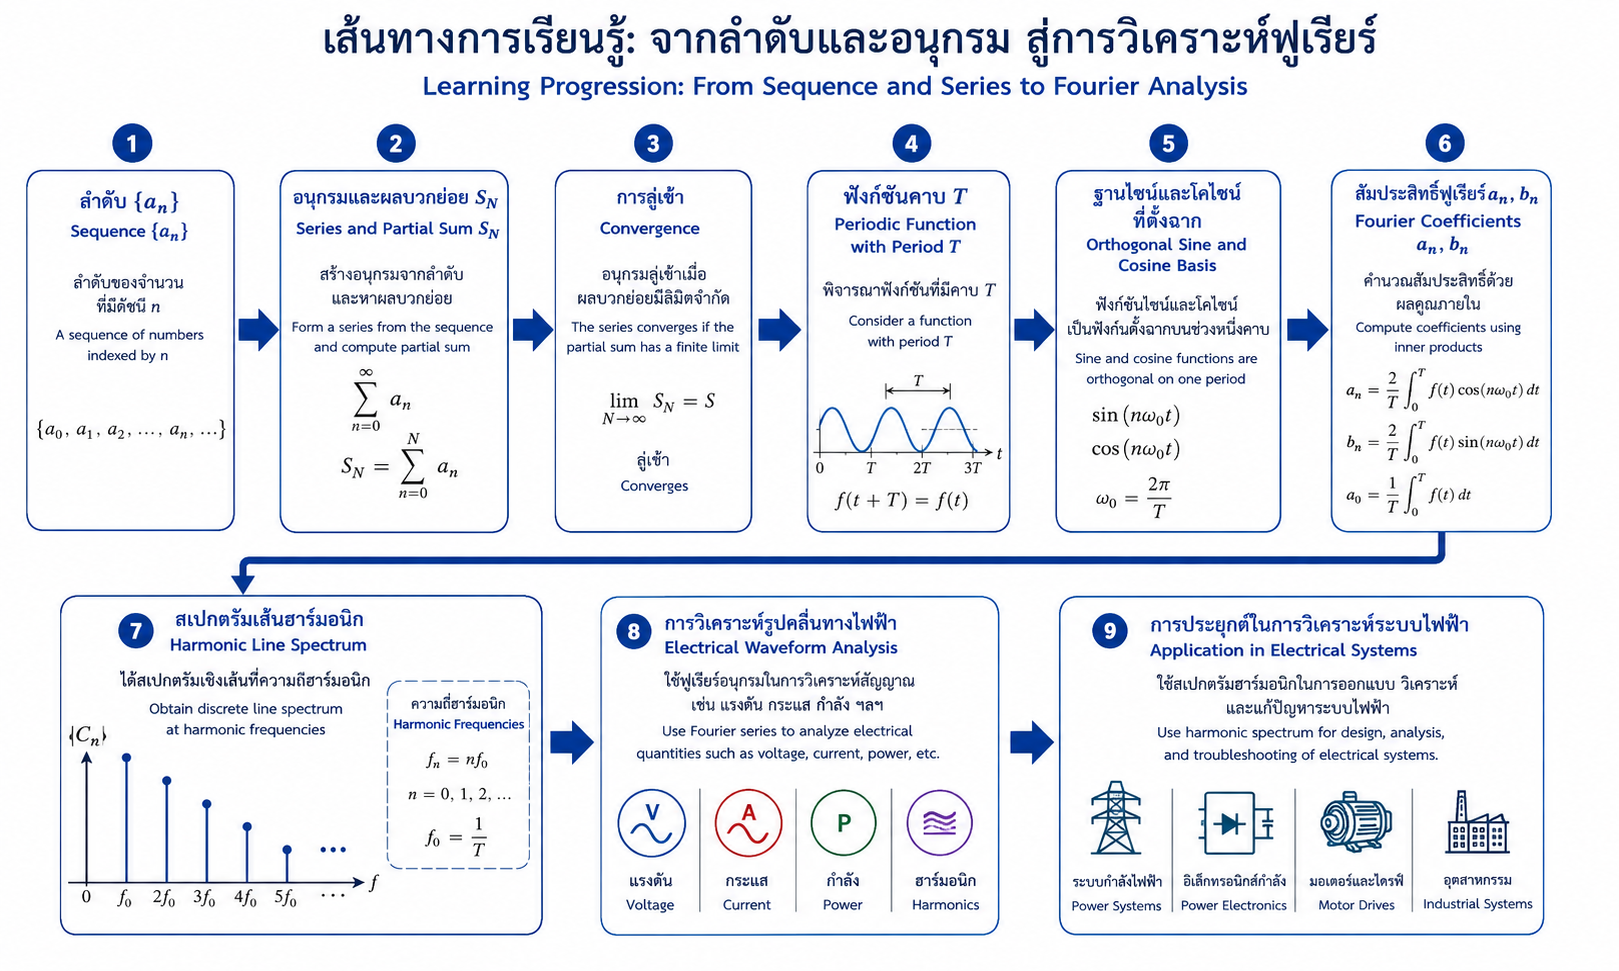
\includegraphics[width=0.8\textwidth]{images/chapter4/figure-01.png}
    \caption{องค์ประกอบพื้นฐานของ Block Diagram}
\end{figure}

\subsubsection{7.2 องค์ประกอบพื้นฐานของ Block Diagram}

Block Diagram ประกอบด้วยองค์ประกอบหลัก 4 ชนิด

\begin{enumerate}
    \item \textbf{บล็อก (Block):} แทนระบบย่อยหนึ่งส่วน กำกับด้วย transfer function เช่น $G(s)$ โดยเอาต์พุตของบล็อกคือผลคูณของอินพุตกับ transfer function ในโดเมน $s$ กล่าวคือ หากอินพุตคือ $X(s)$ เอาต์พุตคือ $Y(s) = G(s)X(s)$
    \item \textbf{เส้นสัญญาณ (Signal Line):} ลูกศรแสดงทิศทางการไหลของสัญญาณ สัญญาณไหลได้ทิศทางเดียวตามลูกศรเท่านั้น
    \item \textbf{จุดรวมสัญญาณ (Summing Junction):} วงกลมที่รวมสัญญาณตั้งแต่สองสัญญาณขึ้นไปด้วยการบวกหรือลบตามเครื่องหมายกำกับที่ทางเข้าแต่ละเส้น เช่น $E(s) = R(s) - B(s)$
    \item \textbf{จุดแยกสัญญาณ (Takeoff Point หรือ Pickoff Point):} จุดที่สัญญาณเดียวกันถูกส่งไปยังหลายเส้นทางพร้อมกันโดยไม่เปลี่ยนแปลงค่า
\end{enumerate}

\subsubsection{7.3 กฎการลดรูปแผนภาพบล็อก}

การลดรูปแผนภาพบล็อก (Block Diagram Reduction) คือกระบวนการรวมบล็อกที่เชื่อมต่อกันตามกฎพีชคณิตทีละขั้นตอน จนเหลือบล็อกเดียวที่แทน transfer function รวมของระบบ กฎพื้นฐานที่ใช้บ่อยที่สุดมี 3 กฎหลัก ได้แก่ การต่อแบบอนุกรม การต่อแบบขนาน และการป้อนกลับ ร่วมกับกฎเสริมอีก 2 กฎสำหรับจัดการตำแหน่งของจุดรวมสัญญาณและจุดแยกสัญญาณเมื่อกฎหลักไม่สามารถใช้ได้โดยตรง

\paragraph{7.3.1 การต่อแบบอนุกรม (Series/Cascade Connection)}

เมื่อบล็อกสองบล็อกต่อกันโดยเอาต์พุตของบล็อกแรกเป็นอินพุตของบล็อกถัดไปโดยตรง (ไม่มีจุดแยกสัญญาณหรือจุดรวมสัญญาณคั่นกลาง) เรียกว่าการต่อแบบอนุกรม transfer function รวมคือผลคูณของ transfer function แต่ละบล็อก

\[
G_{eq}(s) = G_1(s) \, G_2(s)
\]

% [รูปที่ 2: การต่อแบบอนุกรมและผลลัพธ์การลดรูป]
% ประเภทภาพ: Block Diagram
% ตำแหน่งที่แนะนำ: ท้ายหัวข้อ 7.3.1 ก่อนตัวอย่างที่ 1
% วัตถุประสงค์การเรียนรู้: แสดงการแปลงบล็อกสองบล็อกที่ต่ออนุกรมให้เป็นบล็อกเดียว
% คำอธิบายภาพ: แถวบนแสดง $R(s)$ เข้าบล็อก $G_1(s)$ ต่อด้วยบล็อก $G_2(s)$ แล้วออกเป็น $C(s)$ แถวล่างแสดงบล็อกเดียว $G_1(s)G_2(s)$ ที่รับ $R(s)$ และให้ผลลัพธ์ $C(s)$ เท่ากัน พร้อมลูกศร "เทียบเท่ากับ" คั่นกลางสองแถว
% องค์ประกอบที่ต้องมี: บล็อกสี่เหลี่ยมสองบล็อกในแถวบน บล็อกเดียวในแถวล่าง ลูกศรสัญญาณ สัญลักษณ์ "≡" หรือ "เทียบเท่ากับ" คั่นกลาง
% ข้อความหรือป้ายกำกับ: $R(s)$, $C(s)$, $G_1(s)$, $G_2(s)$, $G_1(s)G_2(s)$
% ภาษาของป้ายกำกับ: ไทยและอังกฤษ
% สัดส่วนภาพ: 16:9
% Image Generation Prompt: Control systems block diagram showing two rectangular blocks G1(s) and G2(s) connected in series with an input arrow R(s) and output arrow C(s) in the top row; below, an equivalence arrow points to a single equivalent block labeled G1(s)G2(s) with the same input R(s) and output C(s). Clean minimalist engineering diagram, white background, black lines, clear labels.
% Alt Text: ภาพแสดงบล็อกสองบล็อกต่ออนุกรมกันและบล็อกสมมูลบล็อกเดียวที่มีค่าเท่ากับผลคูณของ transfer function ทั้งสอง

\begin{figure}[htbp]
    \centering
    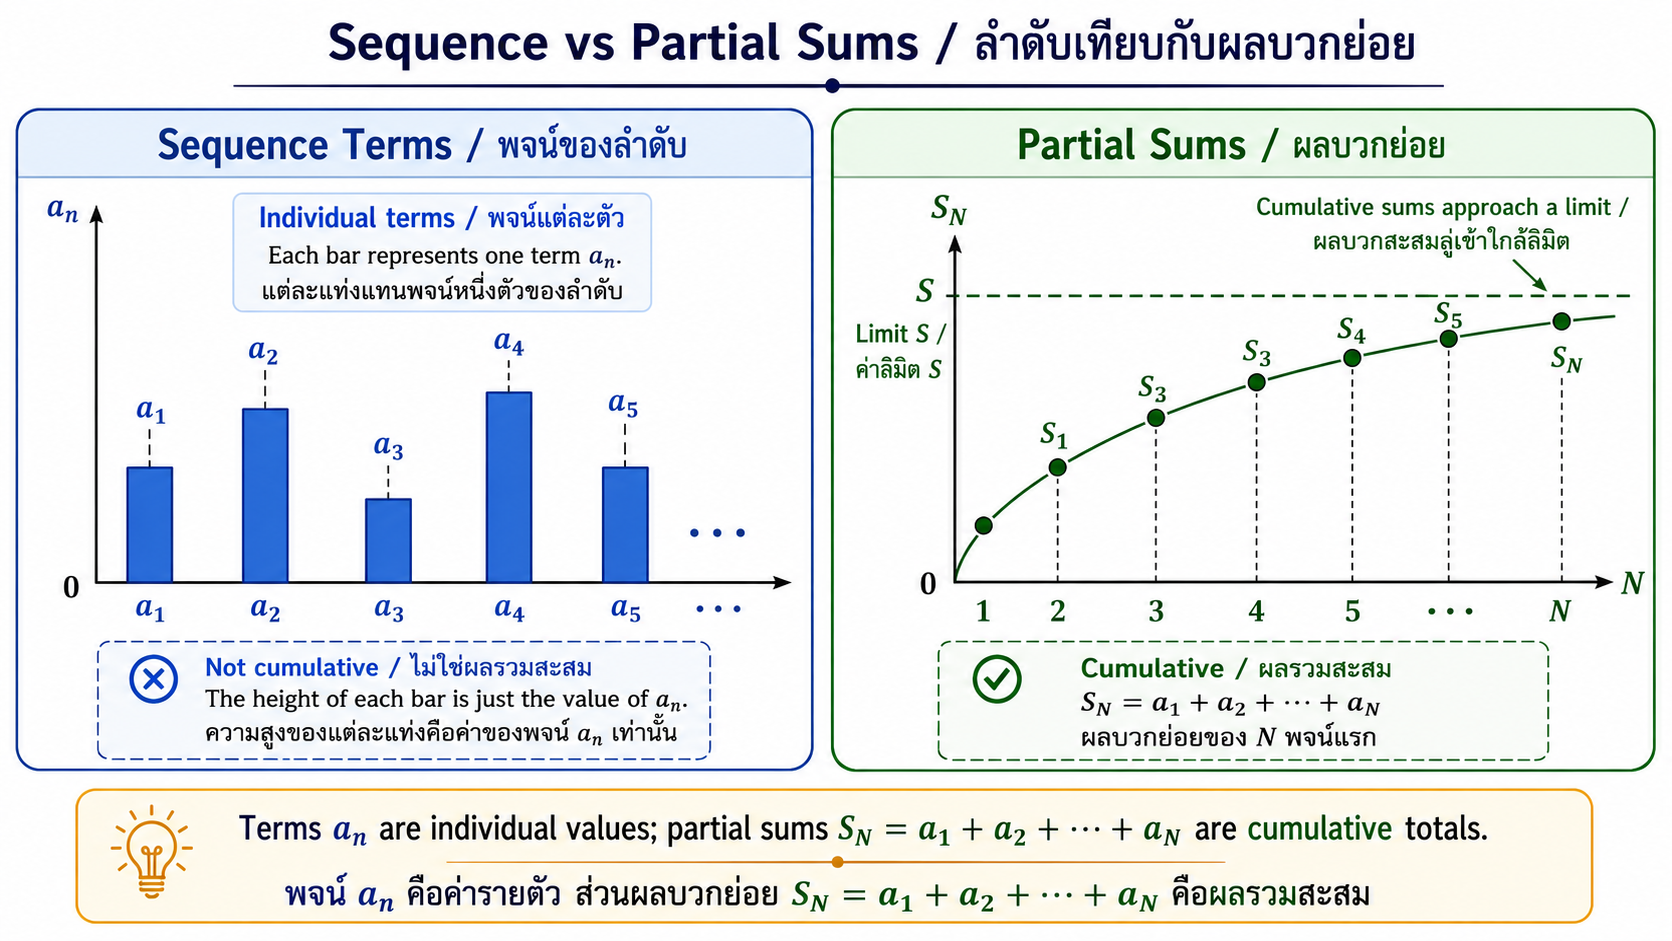
\includegraphics[width=0.8\textwidth]{images/chapter4/figure-02.png}
    \caption{การต่อแบบอนุกรมและผลลัพธ์การลดรูป}
\end{figure}

\textbf{ตัวอย่างที่ 1: การต่อแบบอนุกรม (Series)}

\textbf{โจทย์:} ระบบควบคุมประกอบด้วยตัวควบคุมและพลานต์ต่อกันแบบอนุกรม โดยตัวควบคุมมี transfer function $G_1(s) = \dfrac{1}{s+2}$ และพลานต์มี transfer function $G_2(s) = \dfrac{5}{s+4}$ จงหา transfer function รวม $C(s)/R(s)$

\textit{ขั้นตอนที่ 1 วิเคราะห์ระบบ:} บล็อกทั้งสองต่อกันโดยตรงแบบอนุกรม ไม่มีจุดรวมหรือจุดแยกสัญญาณคั่นกลาง จึงใช้กฎการต่อแบบอนุกรมได้ทันที

\textit{ขั้นตอนที่ 2 กำหนดตัวแปร:} $R(s)$ คืออินพุต $C(s)$ คือเอาต์พุต

\textit{ขั้นตอนที่ 3–4 เลือกกฎและสร้างสมการ:}

\[
G_{eq}(s) = G_1(s)\,G_2(s) = \frac{1}{s+2}\cdot\frac{5}{s+4}
\]

\textit{ขั้นตอนที่ 5–7 จัดรูปและคำนวณ:}

\[
G_{eq}(s) = \frac{5}{(s+2)(s+4)} = \frac{5}{s^2+6s+8}
\]

\textit{ขั้นตอนที่ 8 ตรวจสอบ:} ดีกรีของพหุนามส่วนเท่ากับผลรวมดีกรีของทั้งสองบล็อก (1+1 = 2) สอดคล้องกับสมบัติของระบบอันดับสอง ค่าคงตัวเวลา (time constant) ของแต่ละบล็อกเดิมยังปรากฏเป็นราก $s=-2$ และ $s=-4$ ของสมการส่วน ซึ่งสมเหตุสมผล

\textit{ขั้นตอนที่ 9 แปลความหมาย:} $C(s) = \dfrac{5}{s^2+6s+8}R(s)$ คือ transfer function รวมของตัวควบคุมและพลานต์ที่ต่ออนุกรมกัน พร้อมนำไปวิเคราะห์ในบทถัดไป

\paragraph{7.3.2 การต่อแบบขนาน (Parallel Connection)}

เมื่อบล็อกตั้งแต่สองบล็อกขึ้นไปรับสัญญาณอินพุตเดียวกัน แล้วนำเอาต์พุตของแต่ละบล็อกมารวมกันที่จุดรวมสัญญาณ เรียกว่าการต่อแบบขนาน transfer function รวมคือผลบวก (หรือผลต่าง ตามเครื่องหมายที่จุดรวมสัญญาณ) ของ transfer function แต่ละบล็อก

\[
G_{eq}(s) = G_1(s) \pm G_2(s)
\]

\textbf{ตัวอย่างที่ 2: การต่อแบบขนาน (Parallel)}

\textbf{โจทย์:} ระบบมีสองเส้นทางสัญญาณที่รับอินพุตเดียวกัน $R(s)$ แล้วนำเอาต์พุตมาบวกกันที่จุดรวมสัญญาณ โดย $G_1(s) = \dfrac{3}{s+1}$ และ $G_2(s) = \dfrac{2}{s+5}$ จงหา transfer function รวม $C(s)/R(s)$

\textit{ขั้นตอนที่ 1–2 วิเคราะห์และกำหนดตัวแปร:} ทั้งสองบล็อกรับ $R(s)$ เดียวกัน เอาต์พุตทั้งสองรวมกันเป็น $C(s) = G_1(s)R(s) + G_2(s)R(s)$

\textit{ขั้นตอนที่ 3–4 เลือกกฎและสร้างสมการ:}

\[
G_{eq}(s) = G_1(s) + G_2(s) = \frac{3}{s+1} + \frac{2}{s+5}
\]

\textit{ขั้นตอนที่ 5–7 จัดรูปเศษส่วนร่วมและคำนวณ:}

\[
G_{eq}(s) = \frac{3(s+5) + 2(s+1)}{(s+1)(s+5)} = \frac{3s+15+2s+2}{(s+1)(s+5)} = \frac{5s+17}{s^2+6s+5}
\]

\textit{ขั้นตอนที่ 8 ตรวจสอบ:} ดีกรีของพหุนามเศษต้องน้อยกว่าดีกรีของพหุนามส่วนหนึ่งลำดับ (proper transfer function) ในที่นี้เศษดีกรี 1 ส่วนดีกรี 2 ถูกต้องตามสมบัติของระบบเชิงเหตุ (causal system)

\textit{ขั้นตอนที่ 9 แปลความหมาย:} $G_{eq}(s) = \dfrac{5s+17}{s^2+6s+5}$ คือ transfer function รวมของสองเส้นทางที่ต่อขนานและบวกสัญญาณกันที่เอาต์พุต

\paragraph{7.3.3 การป้อนกลับ (Feedback)}

โครงสร้างป้อนกลับประกอบด้วยบล็อกเส้นทางไปข้างหน้า $G(s)$ (forward path) และบล็อกเส้นทางป้อนกลับ $H(s)$ (feedback path) โดยสัญญาณเอาต์พุตถูกป้อนกลับผ่าน $H(s)$ แล้วนำไปเปรียบเทียบกับสัญญาณอินพุตที่จุดรวมสัญญาณ หาก $H(s)=1$ เรียกว่า \textbf{ระบบป้อนกลับหนึ่งหน่วย (unity feedback)}

สำหรับ \textbf{ระบบป้อนกลับเชิงลบ (negative feedback)} สัญญาณผิดพลาด (error signal) คือ $E(s) = R(s) - H(s)C(s)$ และ $C(s) = G(s)E(s)$ เมื่อแทนค่าและจัดรูปจะได้

\[
\frac{C(s)}{R(s)} = \frac{G(s)}{1 + G(s)H(s)}
\]

ส่วน \textbf{ระบบป้อนกลับเชิงบวก (positive feedback)} ซึ่งสัญญาณป้อนกลับถูกบวกเข้ากับอินพุตแทนการลบ จะได้

\[
\frac{C(s)}{R(s)} = \frac{G(s)}{1 - G(s)H(s)}
\]

พจน์ $G(s)H(s)$ เรียกว่า \textbf{loop gain} ของระบบป้อนกลับ ซึ่งเป็นตัวแปรสำคัญที่ใช้วิเคราะห์เสถียรภาพในบทถัดไป

% [รูปที่ 3: โครงสร้างระบบป้อนกลับเชิงลบและเชิงบวก]
% ประเภทภาพ: Block Diagram
% ตำแหน่งที่แนะนำ: ท้ายหัวข้อ 7.3.3 ก่อนตัวอย่างที่ 3
% วัตถุประสงค์การเรียนรู้: ให้ผู้เรียนแยกแยะโครงสร้างและเครื่องหมายของระบบป้อนกลับเชิงลบกับเชิงบวก
% คำอธิบายภาพ: แสดงจุดรวมสัญญาณรับ $R(s)$ เข้าทางหนึ่งและสัญญาณป้อนกลับจาก $H(s)$ เข้าอีกทางหนึ่ง ผลลัพธ์ $E(s)$ เข้าบล็อก $G(s)$ แล้วออกเป็น $C(s)$ ซึ่งมีจุดแยกสัญญาณย้อนกลับเข้า $H(s)$ ก่อนกลับไปยังจุดรวมสัญญาณ ทำสองแบบคู่กันคือเครื่องหมาย − (เชิงลบ) และเครื่องหมาย + (เชิงบวก)
% องค์ประกอบที่ต้องมี: จุดรวมสัญญาณ บล็อก $G(s)$ บล็อก $H(s)$ จุดแยกสัญญาณ ลูกศรทิศทาง เครื่องหมาย +/−
% ข้อความหรือป้ายกำกับ: $R(s)$, $E(s)$, $C(s)$, $G(s)$, $H(s)$, เครื่องหมาย +, −
% ภาษาของป้ายกำกับ: ไทยและอังกฤษ
% สัดส่วนภาพ: 16:9
% Image Generation Prompt: Two side-by-side control system block diagrams. Left: negative feedback loop with summing junction (R(s) input marked +, feedback marked -) feeding into block G(s) producing output C(s), which splits at a takeoff point back through block H(s) to the summing junction. Right: identical structure but the feedback sign is + for positive feedback. Clean minimalist black-and-white engineering diagram, white background, clear labels.
% Alt Text: ภาพเปรียบเทียบโครงสร้างระบบป้อนกลับเชิงลบและเชิงบวก แสดงตำแหน่งบล็อก G และ H และเครื่องหมายที่จุดรวมสัญญาณ

\begin{figure}[htbp]
    \centering
    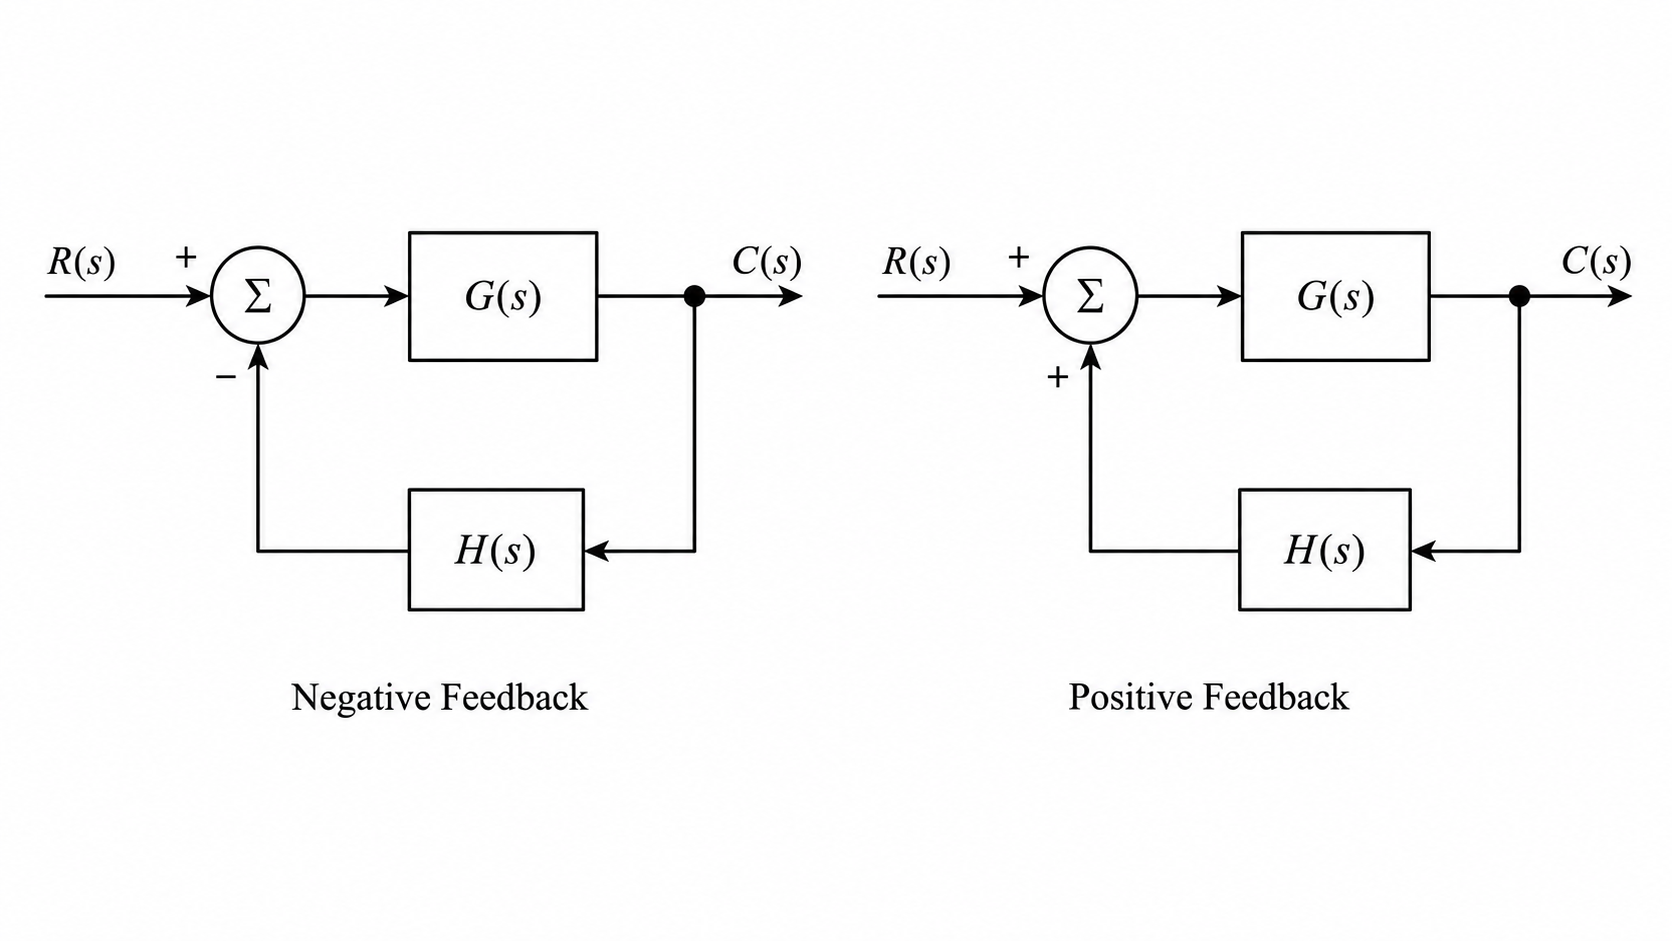
\includegraphics[width=0.8\textwidth]{images/chapter4/figure-03.png}
    \caption{โครงสร้างระบบป้อนกลับเชิงลบและเชิงบวก}
\end{figure}

\textbf{ตัวอย่างที่ 3: การป้อนกลับ (Feedback)}

\textbf{โจทย์:} ระบบควบคุมมีเส้นทางไปข้างหน้า $G(s) = \dfrac{10}{s+2}$ และเส้นทางป้อนกลับเชิงลบ $H(s) = 2$ จงหา closed-loop transfer function $C(s)/R(s)$

\textit{ขั้นตอนที่ 1–2 วิเคราะห์และกำหนดตัวแปร:} เป็นระบบป้อนกลับเชิงลบไม่ใช่หนึ่งหน่วย ($H(s) \neq 1$) สัญญาณผิดพลาด $E(s) = R(s) - H(s)C(s)$

\textit{ขั้นตอนที่ 3–4 เลือกกฎและสร้างสมการ:}

\[
\frac{C(s)}{R(s)} = \frac{G(s)}{1+G(s)H(s)} = \frac{\dfrac{10}{s+2}}{1 + \dfrac{10}{s+2}(2)}
\]

\textit{ขั้นตอนที่ 5–7 จัดรูปและคำนวณ:}

\[
\frac{C(s)}{R(s)} = \frac{\dfrac{10}{s+2}}{\dfrac{s+2+20}{s+2}} = \frac{10}{s+22}
\]

\textit{ขั้นตอนที่ 8 ตรวจสอบ:} ระบบเดิม (open-loop) เป็นระบบอันดับหนึ่งที่มีขั้ว (pole) ที่ $s=-2$ เมื่อปิดลูปป้อนกลับแล้วขั้วเลื่อนไปที่ $s=-22$ ซึ่งอยู่ไกลจากแกนจินตภาพมากขึ้น แสดงว่าระบบตอบสนองเร็วขึ้นเมื่อปิดลูป ซึ่งเป็นผลที่คาดได้จากการป้อนกลับเชิงลบที่มีอัตราขยายสูง

\textit{ขั้นตอนที่ 9 แปลความหมาย:} $\dfrac{C(s)}{R(s)} = \dfrac{10}{s+22}$ คือ closed-loop transfer function ของระบบ ซึ่งจะนำไปใช้วิเคราะห์การตอบสนองในบทที่ว่าด้วยการตอบสนองเชิงเวลา

\paragraph{7.3.4 การเลื่อนจุดรวมสัญญาณ (Moving Summing Junction)}

เมื่อจุดรวมสัญญาณอยู่คนละตำแหน่งกับบล็อกที่ต้องการรวม จำเป็นต้องเลื่อนจุดรวมสัญญาณผ่านบล็อกก่อนจึงจะใช้กฎอนุกรม/ขนาน/ป้อนกลับได้ หลักการคือ \textbf{ค่าที่ไหลผ่านจุดนั้นต้องไม่เปลี่ยนแปลง}

\begin{itemize}
    \item \textbf{เลื่อนจุดรวมสัญญาณไปด้านหลังบล็อก:} ต้องเพิ่มบล็อก $G(s)$ เข้าที่สัญญาณอีกเส้นที่เข้าจุดรวมสัญญาณนั้น เพื่อชดเชยผลของการย้าย
    \item \textbf{เลื่อนจุดรวมสัญญาณไปด้านหน้าบล็อก:} ต้องเพิ่มบล็อก $1/G(s)$ เข้าที่สัญญาณอีกเส้นแทน
\end{itemize}

% [รูปที่ 4: การเลื่อนจุดรวมสัญญาณไปด้านหน้าและด้านหลังบล็อก]
% ประเภทภาพ: Block Diagram
% ตำแหน่งที่แนะนำ: ท้ายหัวข้อ 7.3.4
% วัตถุประสงค์การเรียนรู้: แสดงว่าเมื่อเลื่อนจุดรวมสัญญาณผ่านบล็อก ต้องเพิ่มหรือหารด้วย $G(s)$ ที่สัญญาณอีกเส้นเพื่อให้ค่าที่จุดรวมสัญญาณเดิมไม่เปลี่ยนแปลง
% คำอธิบายภาพ: แถวบนแสดงบล็อก $G(s)$ ตามด้วยจุดรวมสัญญาณที่มีสัญญาณ $X(s)$ เข้ามาบวก แถวล่างแสดงจุดรวมสัญญาณย้ายมาก่อนบล็อก $G(s)$ พร้อมสัญญาณ $X(s)$ ที่ถูกส่งผ่านบล็อกเพิ่มเติม $1/G(s)$ ก่อนเข้าจุดรวมสัญญาณ เพื่อให้ผลลัพธ์เอาต์พุตเท่าเดิม
% องค์ประกอบที่ต้องมี: บล็อกสี่เหลี่ยม จุดรวมสัญญาณ บล็อกเสริม $1/G(s)$ หรือ $G(s)$ ลูกศรทิศทาง
% ข้อความหรือป้ายกำกับ: $G(s)$, $1/G(s)$, $X(s)$, เครื่องหมาย +
% ภาษาของป้ายกำกับ: ไทยและอังกฤษ
% สัดส่วนภาพ: 4:3
% Image Generation Prompt: Control systems block diagram equivalence pair showing a summing junction being moved across a block G(s): top diagram has block G(s) followed by a summing junction adding signal X(s); bottom equivalent diagram has the summing junction moved before block G(s), with signal X(s) now passed through an added block 1/G(s) before summation. Clean minimalist engineering diagram style, white background, black lines.
% Alt Text: ภาพแสดงกฎการเลื่อนจุดรวมสัญญาณผ่านบล็อกโดยต้องเพิ่มบล็อกชดเชย 1 ส่วน G(s)

\begin{figure}[htbp]
    \centering
    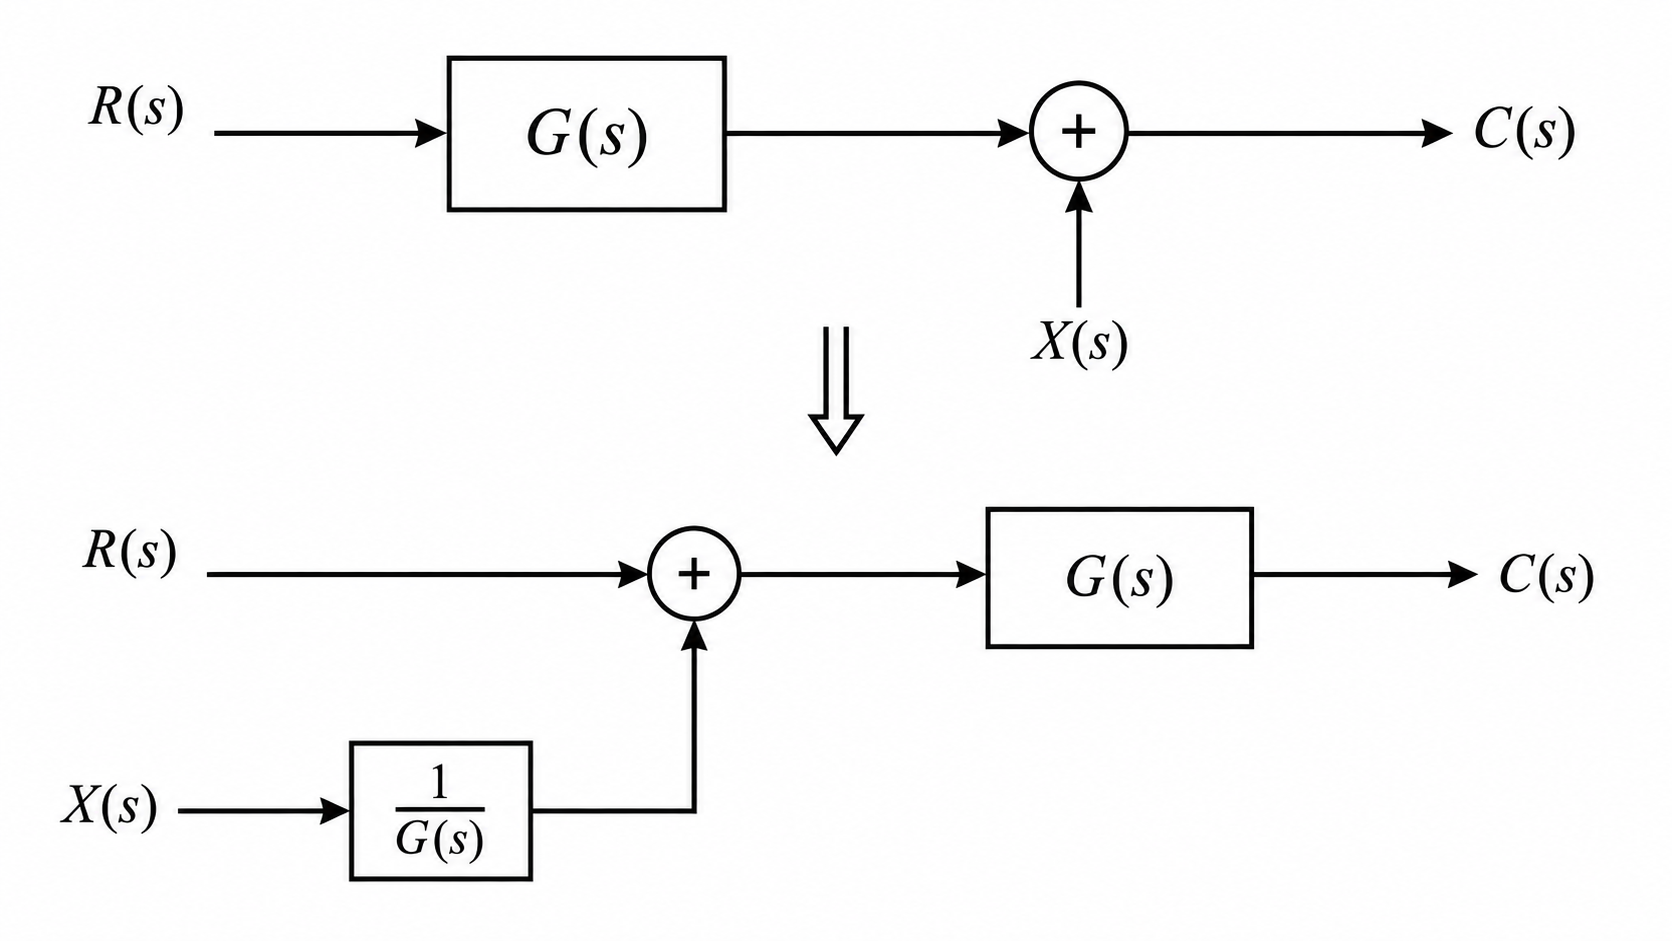
\includegraphics[width=0.8\textwidth]{images/chapter4/figure-04.png}
    \caption{การเลื่อนจุดรวมสัญญาณไปด้านหน้าและด้านหลังบล็อก}
\end{figure}

\paragraph{7.3.5 การเลื่อนจุดแยกสัญญาณ (Moving Takeoff Point)}

ในทำนองเดียวกัน เมื่อจุดแยกสัญญาณอยู่คนละตำแหน่งกับบล็อกที่ต้องการรวม สามารถเลื่อนได้โดยยังคงหลักการเดิมคือค่าที่แยกออกไปต้องไม่เปลี่ยนแปลง

\begin{itemize}
    \item \textbf{เลื่อนจุดแยกสัญญาณไปด้านหลังบล็อก:} ต้องเพิ่มบล็อก $1/G(s)$ เข้าที่เส้นสัญญาณที่แยกออกไป
    \item \textbf{เลื่อนจุดแยกสัญญาณไปด้านหน้าบล็อก:} ต้องเพิ่มบล็อก $G(s)$ เข้าที่เส้นสัญญาณที่แยกออกไปแทน
\end{itemize}

% [รูปที่ 5: การเลื่อนจุดแยกสัญญาณไปด้านหน้าและด้านหลังบล็อก]
% ประเภทภาพ: Block Diagram
% ตำแหน่งที่แนะนำ: ท้ายหัวข้อ 7.3.5
% วัตถุประสงค์การเรียนรู้: แสดงว่าเมื่อเลื่อนจุดแยกสัญญาณผ่านบล็อก ต้องเพิ่มบล็อกชดเชยที่เส้นแยกเพื่อรักษาค่าสัญญาณเดิม
% คำอธิบายภาพ: แถวบนแสดงบล็อก $G(s)$ แล้วจึงมีจุดแยกสัญญาณแยกเอาต์พุตออกไปเป็น $Y(s)$ แถวล่างแสดงจุดแยกสัญญาณย้ายมาก่อนบล็อก $G(s)$ พร้อมเพิ่มบล็อก $G(s)$ อีกตัวในเส้นที่แยกออกไปเพื่อให้ค่า $Y(s)$ เท่าเดิม
% องค์ประกอบที่ต้องมี: บล็อกสี่เหลี่ยม จุดแยกสัญญาณ บล็อกเสริม $G(s)$ หรือ $1/G(s)$ ลูกศรทิศทาง
% ข้อความหรือป้ายกำกับ: $G(s)$, $1/G(s)$, $Y(s)$
% ภาษาของป้ายกำกับ: ไทยและอังกฤษ
% สัดส่วนภาพ: 4:3
% Image Generation Prompt: Control systems block diagram equivalence pair showing a takeoff point being moved across a block G(s): top diagram has block G(s) followed by a takeoff point branching signal Y(s); bottom equivalent diagram has the takeoff point moved before block G(s), with an added block G(s) inserted in the branched line so Y(s) stays identical. Clean minimalist engineering diagram style, white background, black lines.
% Alt Text: ภาพแสดงกฎการเลื่อนจุดแยกสัญญาณผ่านบล็อกโดยต้องเพิ่มบล็อกชดเชย G(s)

\begin{figure}[htbp]
    \centering
    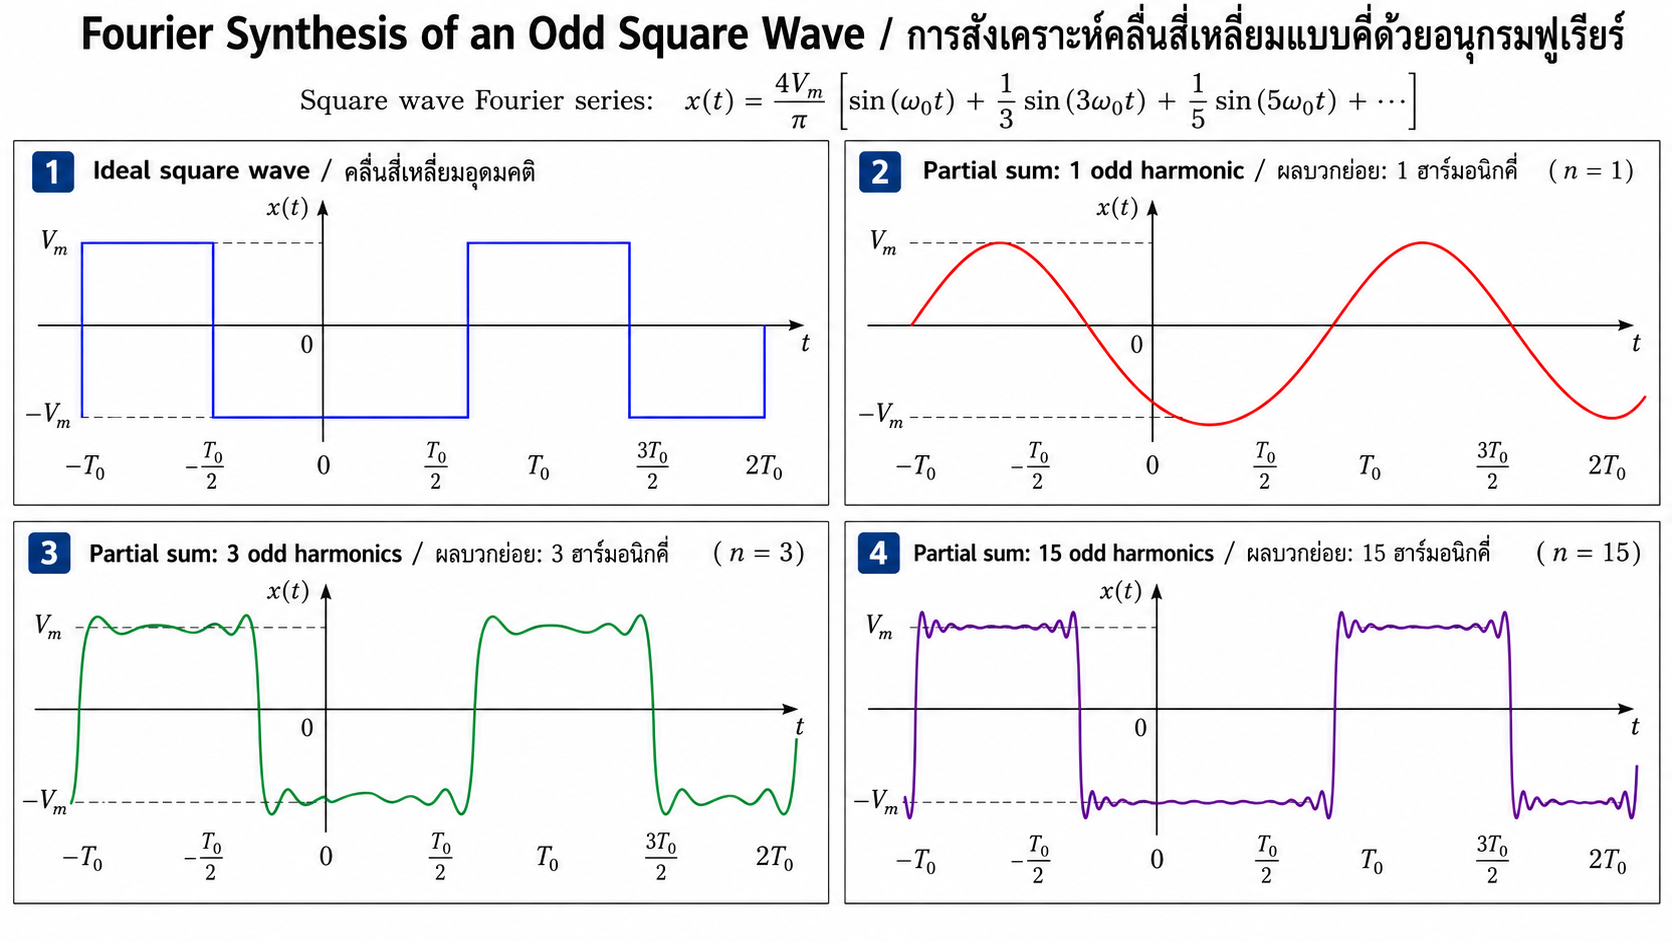
\includegraphics[width=0.8\textwidth]{images/chapter4/figure-05.png}
    \caption{การเลื่อนจุดแยกสัญญาณไปด้านหน้าและด้านหลังบล็อก}
\end{figure}


\textbf{ตารางที่ 3} สรุปกฎการลดรูปแผนภาพบล็อกที่ใช้บ่อย

\begin{table}[htbp]
    \centering
    \begin{tabularx}{\textwidth}{L{0.23\textwidth} Y Y}
        \hline
        \textbf{กฎ} & \textbf{โครงสร้างเดิม} & \textbf{ผลลัพธ์หลังลดรูป} \\
        \hline
        การต่อแบบอนุกรม & $G_1(s)$ ตามด้วย $G_2(s)$ & $G_1(s)G_2(s)$ \\
        การต่อแบบขนาน & $G_1(s)$ และ $G_2(s)$ รับอินพุตเดียวกัน บวกที่เอาต์พุต & $G_1(s) \pm G_2(s)$ \\
        การป้อนกลับเชิงลบ & $G(s)$ ในเส้นไปข้างหน้า, $H(s)$ ป้อนกลับลบ & $\dfrac{G(s)}{1+G(s)H(s)}$ \\
        การป้อนกลับเชิงบวก & $G(s)$ ในเส้นไปข้างหน้า, $H(s)$ ป้อนกลับบวก & $\dfrac{G(s)}{1-G(s)H(s)}$ \\
        เลื่อนจุดรวมสัญญาณไปด้านหลังบล็อก & จุดรวมสัญญาณอยู่หน้าบล็อก $G(s)$ & เพิ่มบล็อก $G(s)$ ที่สัญญาณอีกเส้น \\
        เลื่อนจุดรวมสัญญาณไปด้านหน้าบล็อก & จุดรวมสัญญาณอยู่หลังบล็อก $G(s)$ & เพิ่มบล็อก $1/G(s)$ ที่สัญญาณอีกเส้น \\
        เลื่อนจุดแยกสัญญาณไปด้านหลังบล็อก & จุดแยกสัญญาณอยู่หน้าบล็อก $G(s)$ & เพิ่มบล็อก $1/G(s)$ ที่เส้นแยก \\
        เลื่อนจุดแยกสัญญาณไปด้านหน้าบล็อก & จุดแยกสัญญาณอยู่หลังบล็อก $G(s)$ & เพิ่มบล็อก $G(s)$ ที่เส้นแยก \\
        \hline
    \end{tabularx}
\end{table}


\subsubsection{7.4 ขั้นตอนการลดรูปแผนภาพบล็อกที่มีหลายลูปซ้อนกัน}

ระบบควบคุมจริงมักมีลูปป้อนกลับซ้อนกันหลายชั้น (multiple nested loops) ซึ่งไม่สามารถใช้กฎอนุกรม ขนาน หรือป้อนกลับได้ทันทีเพราะมีจุดรวมสัญญาณหรือจุดแยกสัญญาณคั่นอยู่ระหว่างบล็อก แนวทางที่แนะนำสำหรับการลดรูปแผนภาพบล็อกที่ซับซ้อนมีลำดับขั้นตอนดังนี้

\begin{enumerate}
    \item \textbf{รวมบล็อกอนุกรมและขนานที่ไม่มีจุดรวม/จุดแยกสัญญาณคั่นกลาง} ให้เหลือน้อยบล็อกที่สุดก่อน
    \item \textbf{เลื่อนจุดรวมสัญญาณหรือจุดแยกสัญญาณ} (ตามหัวข้อ 7.3.4–7.3.5) เพื่อให้จุดรวม/จุดแยกสัญญาณที่ขวางอยู่เคลื่อนออกจากลูปด้านใน
    \item \textbf{ลดรูปลูปป้อนกลับที่อยู่ด้านในสุดก่อน} โดยใช้สูตร $G/(1\pm GH)$ แล้วแทนที่ลูปนั้นด้วยบล็อกสมมูลบล็อกเดียว
    \item \textbf{ทำซ้ำขั้นตอนที่ 1–3} จากลูปในสุดไล่ออกไปยังลูปนอกสุด จนเหลือแผนภาพที่มีเพียงเส้นทางไปข้างหน้าเส้นเดียวกับลูปป้อนกลับหลักเพียงลูปเดียว
    \item \textbf{ใช้กฎการป้อนกลับ} ลดรูปลูปสุดท้ายให้เหลือบล็อกเดียว ซึ่งคือ transfer function รวมของทั้งระบบ
\end{enumerate}

ข้อควรระวังที่สำคัญคือ \textbf{ควรลดรูปลูปในสุดก่อนเสมอ} และหลีกเลี่ยงการเลื่อนจุดรวมสัญญาณผ่านจุดแยกสัญญาณ (หรือในทางกลับกัน) เนื่องจากลำดับการดำเนินการทั้งสองไม่สามารถสลับกันได้โดยทั่วไป หากแผนภาพมีจุดรวมสัญญาณและจุดแยกสัญญาณสลับซับซ้อนกันมาก ควรพิจารณาแปลงเป็น Signal Flow Graph และใช้ Mason's Gain Formula แทน ซึ่งจะกล่าวถึงในหัวข้อถัดไป

\subsubsection{7.5 Signal Flow Graph (SFG)}

\textbf{Signal Flow Graph (SFG)} เป็นอีกแนวทางหนึ่งในการแทนความสัมพันธ์เชิงเส้นระหว่างตัวแปรของระบบด้วยกราฟทิศทาง (directed graph) แทนที่จะใช้บล็อกสี่เหลี่ยมและจุดรวม/จุดแยกสัญญาณแบบ Block Diagram โดยทุกความสัมพันธ์เชิงเส้นสามารถแปลงเป็น SFG ได้เสมอ และทุก SFG สามารถแปลงกลับเป็น Block Diagram ได้เช่นกัน ข้อได้เปรียบสำคัญของ SFG คือสามารถหา transfer function รวมได้โดยตรงจากโครงสร้างกราฟด้วย \textbf{Mason's Gain Formula} โดยไม่ต้องลดรูปทีละขั้นตอนเหมือน Block Diagram

\paragraph{7.5.1 Node และ Branch}

\begin{itemize}
    \item \textbf{โหนด (Node):} จุดที่แทนตัวแปรหรือสัญญาณหนึ่งตัวในระบบ เช่น $R(s)$, $E(s)$, $C(s)$ ค่าของโหนดหนึ่งเท่ากับผลรวมของสัญญาณทั้งหมดที่ไหลเข้าสู่โหนดนั้นตามกิ่งที่เชื่อมเข้ามา
    \item \textbf{กิ่ง (Branch):} เส้นเชื่อมมีทิศทางระหว่างสองโหนด กำกับด้วยค่าอัตราขยาย (gain หรือ transmittance) ของกิ่งนั้น สัญญาณที่โหนดปลายทางเท่ากับสัญญาณที่โหนดต้นทางคูณด้วยอัตราขยายของกิ่ง
\end{itemize}

\paragraph{7.5.2 Path และ Forward Path}

\begin{itemize}
    \item \textbf{เส้นทาง (Path):} ลำดับของกิ่งที่เชื่อมต่อกันตามทิศทางลูกศรอย่างต่อเนื่องโดยไม่ผ่านโหนดใดซ้ำ
    \item \textbf{เส้นทางหน้า (Forward Path):} เส้นทางที่เริ่มจากโหนดอินพุต (source node) ไปสิ้นสุดที่โหนดเอาต์พุต (sink node) โดยไม่ผ่านโหนดใดซ้ำ อัตราขยายของเส้นทางหน้า ($P_k$) คือผลคูณของอัตราขยายกิ่งทั้งหมดที่ประกอบเป็นเส้นทางนั้น
\end{itemize}

\paragraph{7.5.3 Loop และ Loop Gain}

\textbf{ลูป (Loop):} เส้นทางปิดที่เริ่มต้นและสิ้นสุดที่โหนดเดียวกัน โดยไม่ผ่านโหนดอื่นซ้ำระหว่างทาง \textbf{อัตราขยายลูป (Loop Gain)} คือผลคูณของอัตราขยายกิ่งทั้งหมดที่ประกอบเป็นลูปนั้น

\paragraph{7.5.4 Non-touching Loop}

ลูปตั้งแต่สองลูปขึ้นไปเรียกว่า \textbf{ลูปไม่สัมผัสกัน (Non-touching Loop)} เมื่อลูปเหล่านั้น\textbf{ไม่มีโหนดร่วมกันเลย} แนวคิดนี้เป็นหัวใจสำคัญของ Mason's Gain Formula เนื่องจากค่าดีเทอร์มิแนนต์ของกราฟต้องคำนึงถึงผลคูณของอัตราขยายของลูปที่ไม่สัมผัสกันด้วย ในทางกลับกัน หากเส้นทางหน้าหรือลูปใดมีโหนดร่วมกับลูปอื่น จะเรียกว่า\textbf{สัมผัสกัน (touching)}

% [รูปที่ 6: Signal Flow Graph แสดง Node, Branch, Forward Path และ Loop]
% ประเภทภาพ: Technical Illustration
% ตำแหน่งที่แนะนำ: ท้ายหัวข้อ 7.5.4
% วัตถุประสงค์การเรียนรู้: ให้ผู้เรียนระบุ Node, Branch, Forward Path และ Loop บน Signal Flow Graph ได้ถูกต้อง
% คำอธิบายภาพ: แสดงกราฟที่มีโหนดเรียงจากซ้ายไปขวา ได้แก่ $R$, $1$, $2$, $3$, $C$ เชื่อมด้วยกิ่งกำกับอัตราขยาย $G_1$, $G_2$, $G_3$ ตามลำดับ (เส้นทางหน้า) และมีกิ่งย้อนกลับจากโหนด 2 กลับไปโหนด 1 กำกับด้วย $-H_1$ แสดงเป็นลูป วงกลมประแนวเส้นทางหน้าด้วยสีหนึ่ง และวงกลมลูปด้วยเส้นประอีกสีหนึ่ง พร้อมป้ายกำกับ "Forward Path" และ "Loop"
% องค์ประกอบที่ต้องมี: โหนดวงกลมเล็ก 5 โหนด กิ่งลูกศรกำกับอัตราขยาย กิ่งย้อนกลับแสดงลูป เส้นประเน้นเส้นทางหน้าและลูป ป้ายกำกับภาษาไทย/อังกฤษ
% ข้อความหรือป้ายกำกับ: $R$, $C$, $G_1$, $G_2$, $G_3$, $-H_1$, "Forward Path", "Loop"
% ภาษาของป้ายกำกับ: ไทยและอังกฤษ
% สัดส่วนภาพ: 16:9
% Image Generation Prompt: Signal flow graph diagram for a control systems textbook: five small circular nodes labeled R, 1, 2, 3, C arranged left to right, connected by directed arrows (branches) labeled G1, G2, G3 forming the main chain, plus one feedback arrow curving from node 2 back to node 1 labeled -H1 forming a loop. Highlight the forward path chain with a dashed overlay labeled "Forward Path" and the feedback loop with a different dashed overlay labeled "Loop". Clean minimalist black-and-white engineering diagram, white background.
% Alt Text: ภาพกราฟการไหลของสัญญาณแสดงโหนด กิ่ง เส้นทางหน้า และลูปป้อนกลับ

\begin{figure}[htbp]
    \centering
    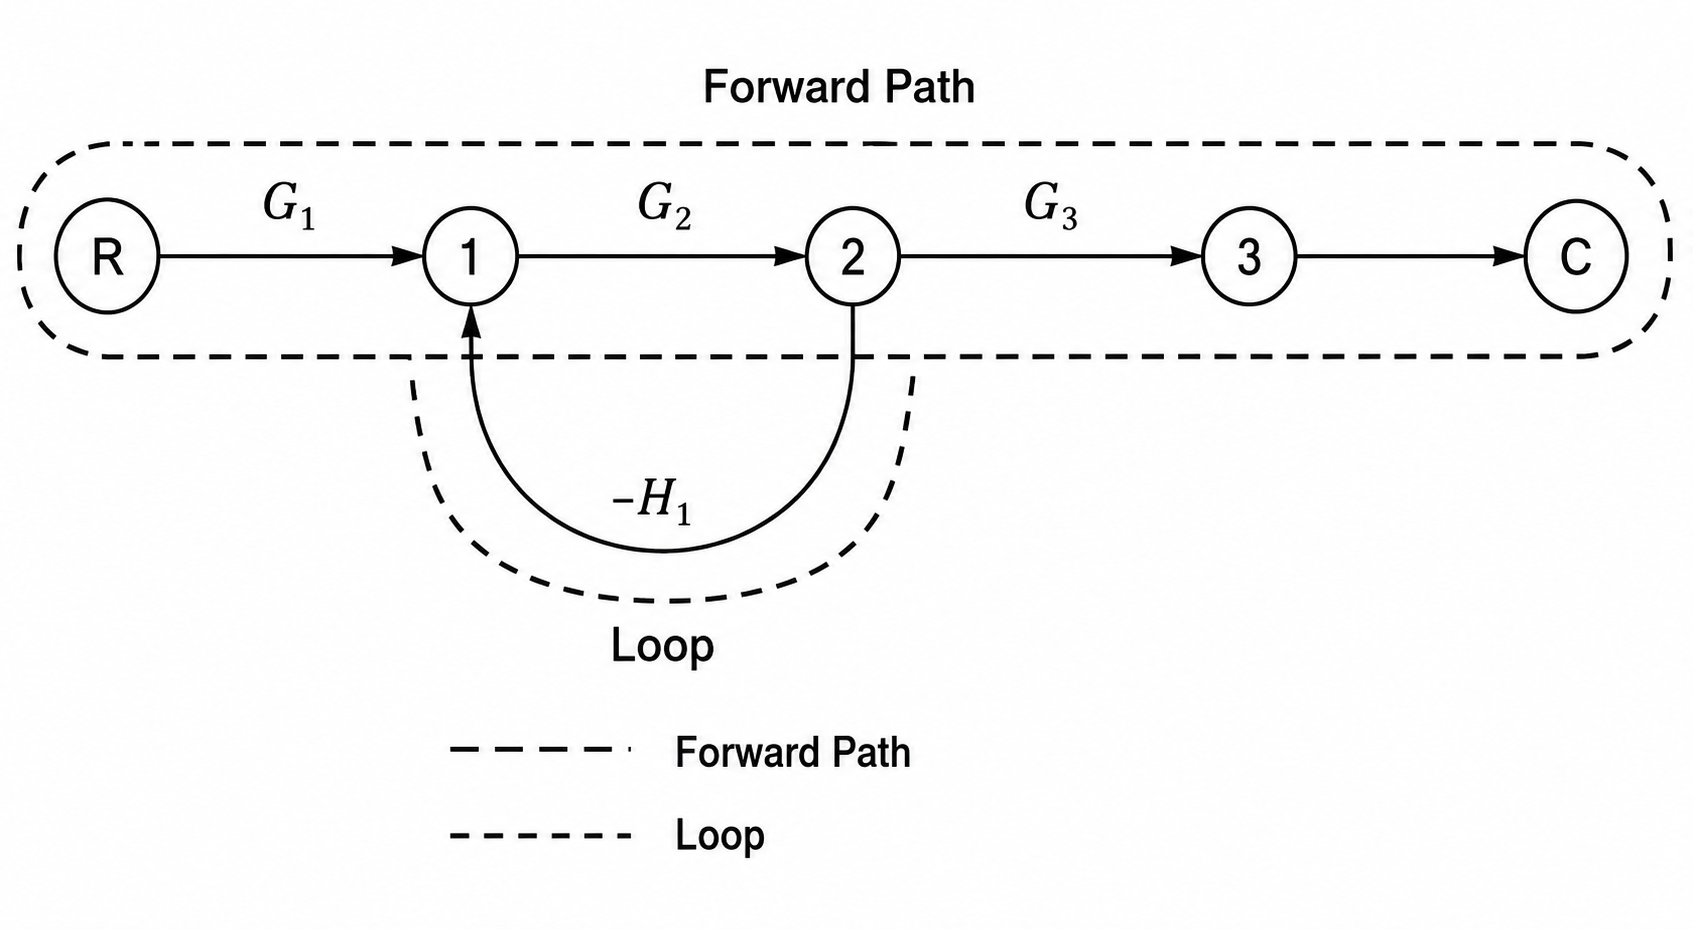
\includegraphics[width=0.8\textwidth]{images/chapter4/figure-06.png}
    \caption{Signal Flow Graph แสดง Node, Branch, Forward Path และ Loop}
\end{figure}

\subsubsection{7.6 Mason's Gain Formula}

\textbf{Mason's Gain Formula} เป็นสูตรที่ใช้คำนวณอัตราขยายรวม (overall transfer function) ระหว่างโหนดอินพุตกับโหนดเอาต์พุตของ Signal Flow Graph ได้โดยตรงจากโครงสร้างกราฟ โดยไม่ต้องลดรูปทีละขั้นตอน สูตรมีรูปแบบดังนี้

\[
P = \frac{C(s)}{R(s)} = \frac{1}{\Delta}\sum_{k} P_k \, \Delta_k
\]

โดยที่

\begin{itemize}
    \item $P$ คือ transfer function รวมระหว่างโหนดอินพุตกับโหนดเอาต์พุต
    \item $P_k$ คืออัตราขยายของเส้นทางหน้าเส้นที่ $k$
    \item $\Delta$ คือ \textbf{ดีเทอร์มิแนนต์ของกราฟ (graph determinant)} คำนวณจาก
\end{itemize}

\[
\Delta = 1 - \sum L_i + \sum L_iL_j - \sum L_iL_jL_k + \cdots
\]

โดย $\sum L_i$ คือผลรวมของอัตราขยายลูปทั้งหมด $\sum L_iL_j$ คือผลรวมของผลคูณอัตราขยายของทุกคู่ลูปที่ไม่สัมผัสกัน $\sum L_iL_jL_k$ คือผลรวมของผลคูณอัตราขยายของทุกกลุ่มสามลูปที่ไม่สัมผัสกัน และเป็นเช่นนี้ต่อไปสำหรับกลุ่มลูปที่ไม่สัมผัสกันจำนวนมากขึ้น

\begin{itemize}
    \item $\Delta_k$ คือ \textbf{โคแฟกเตอร์ของเส้นทางหน้าที่ $k$ (path cofactor)} ซึ่งคำนวณเหมือน $\Delta$ แต่พิจารณาเฉพาะส่วนของกราฟที่\textbf{ไม่สัมผัส}กับเส้นทางหน้าที่ $k$ นั้น กล่าวคือ ตัดลูปทุกลูปที่มีโหนดร่วมกับเส้นทางหน้าที่ $k$ ออกก่อนคำนวณ
\end{itemize}

\textbf{ขั้นตอนการคำนวณด้วย Mason's Gain Formula}

\begin{enumerate}
    \item เขียน Signal Flow Graph ของระบบให้ครบถ้วน กำกับอัตราขยายทุกกิ่ง
    \item ระบุเส้นทางหน้าทั้งหมดและคำนวณอัตราขยาย $P_k$ ของแต่ละเส้นทาง
    \item ระบุลูปทั้งหมดในกราฟและคำนวณอัตราขยายลูปแต่ละลูป
    \item ตรวจสอบคู่ กลุ่มสาม ฯลฯ ของลูปที่ไม่สัมผัสกัน (ไม่มีโหนดร่วมกัน)
    \item คำนวณดีเทอร์มิแนนต์ $\Delta$ จากผลรวมและผลคูณตามสูตร
    \item คำนวณโคแฟกเตอร์ $\Delta_k$ ของแต่ละเส้นทางหน้า โดยตัดลูปที่สัมผัสกับเส้นทางนั้นออก
    \item แทนค่า $P_k$ และ $\Delta_k$ ลงในสูตรและรวมผลทุกเส้นทาง แล้วหารด้วย $\Delta$
    \item จัดรูปและตรวจสอบผลลัพธ์ให้อยู่ในรูป transfer function ที่เป็นเศษส่วนของพหุนามใน $s$
\end{enumerate}


% [รูปที่ 7: Signal Flow Graph สำหรับตัวอย่างที่ 4 การประยุกต์ใช้ Mason's Gain Formula]
% ประเภทภาพ: Technical Illustration
% ตำแหน่งที่แนะนำ: ก่อนตัวอย่างที่ 4
% วัตถุประสงค์การเรียนรู้: ให้ผู้เรียนเห็นโครงสร้างกราฟที่มีสองเส้นทางหน้าและสองลูปไม่สัมผัสกัน ก่อนฝึกคำนวณด้วย Mason's Gain Formula
% คำอธิบายภาพ: แสดงโหนด $R$, $1$, $2$, $3$, $4$, $5$, $C$ โดยเส้นทางหน้าที่หนึ่งไหลจาก $R \to 1 \to 2 \to 3 \to 4 \to C$ กำกับอัตราขยาย $G_1, G_2, G_3, G_4, G_5$ ตามลำดับ เส้นทางหน้าที่สองไหลจาก $R \to 5 \to 4 \to C$ กำกับอัตราขยาย $G_6, G_7, G_5$ มีลูป $L_1$ จากโหนด 2 กลับไปโหนด 1 กำกับ $-H_1$ และลูป $L_2$ จากโหนด 4 กลับไปโหนด 3 กำกับ $-H_2$ ระบายสีหรือเส้นประแยกลูปทั้งสองให้เห็นชัดว่าไม่มีโหนดร่วมกัน
% องค์ประกอบที่ต้องมี: โหนด 7 โหนด กิ่งกำกับอัตราขยายครบทุกกิ่ง ลูกศรทิศทาง เส้นประหรือสีแยกลูป $L_1$ และ $L_2$
% ข้อความหรือป้ายกำกับ: $R$, $C$, $1$-$5$, $G_1$-$G_7$, $-H_1$, $-H_2$
% ภาษาของป้ายกำกับ: ไทยและอังกฤษ
% สัดส่วนภาพ: 16:9
% Image Generation Prompt: Signal flow graph for a control systems worked example: nodes R, 1, 2, 3, 4, 5, C. Main chain forward path R-1-2-3-4-C with branch gains G1, G2, G3, G4, G5. Second forward path R-5-4-C with branch gains G6, G7 feeding into node 4 then G5 to C. A feedback loop from node 2 back to node 1 labeled -H1, and a separate feedback loop from node 4 back to node 3 labeled -H2, drawn with distinct dashed colors to show they share no common nodes. Clean minimalist black-and-white engineering diagram, white background, clear labels.
% Alt Text: ภาพกราฟการไหลของสัญญาณที่มีสองเส้นทางหน้าและสองลูปป้อนกลับที่ไม่สัมผัสกัน ใช้ประกอบตัวอย่างการคำนวณด้วยสูตรเมสัน

\begin{figure}[htbp]
    \centering
    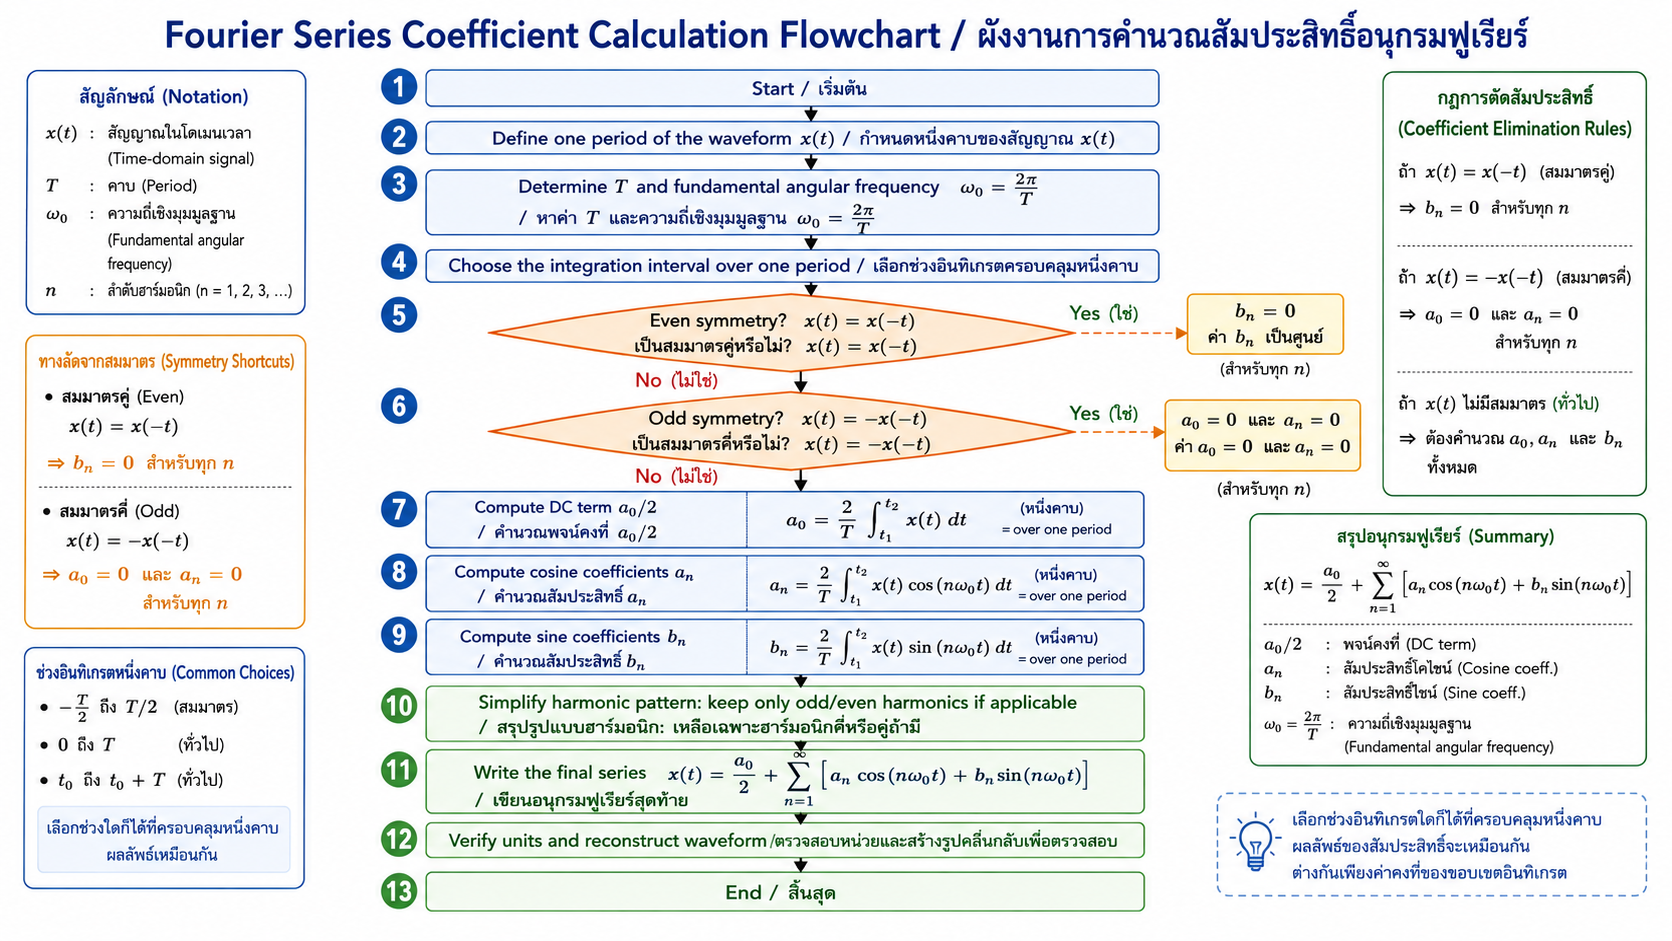
\includegraphics[width=0.8\textwidth]{images/chapter4/figure-07.png}
    \caption{Signal Flow Graph สำหรับตัวอย่างที่ 4 การประยุกต์ใช้ Mason's Gain Formula}
\end{figure}

\textbf{ตัวอย่างที่ 4: การประยุกต์ใช้ Mason's Gain Formula}

\textbf{โจทย์:} Signal Flow Graph ของระบบหนึ่งมีโหนดอินพุต $R$ และโหนดเอาต์พุต $C$ ประกอบด้วย

\begin{itemize}
    \item เส้นทางหน้าที่ 1: $R \to 1 \to 2 \to 3 \to 4 \to C$ อัตราขยายกิ่งตามลำดับคือ $G_1, G_2, G_3, G_4, G_5$
    \item เส้นทางหน้าที่ 2: $R \to 5 \to 4 \to C$ อัตราขยายกิ่งตามลำดับคือ $G_6, G_7$ (เข้าสู่โหนด 4) แล้วออกด้วยกิ่งเดิม $G_5$
    \item ลูป $L_1$: จากโหนด 2 กลับไปโหนด 1 อัตราขยาย $-H_1$ (ประกอบด้วยกิ่ง $G_2$ และกิ่งย้อนกลับ $-H_1$)
    \item ลูป $L_2$: จากโหนด 4 กลับไปโหนด 3 อัตราขยาย $-H_2$ (ประกอบด้วยกิ่ง $G_4$ และกิ่งย้อนกลับ $-H_2$)
\end{itemize}

จงหา transfer function รวม $C(s)/R(s)$ ด้วย Mason's Gain Formula

\textit{ขั้นตอนที่ 1 เขียน SFG:} ตามรูปที่ 7

\textit{ขั้นตอนที่ 2 ระบุเส้นทางหน้าและคำนวณ $P_k$:}

\[
P_1 = G_1G_2G_3G_4G_5, \qquad P_2 = G_6G_7G_5
\]

\textit{ขั้นตอนที่ 3 ระบุลูปและคำนวณอัตราขยายลูป:}

ลูป $L_1$ ประกอบด้วยกิ่ง $1\to2$ (อัตราขยาย $G_2$) และกิ่งย้อนกลับ $2\to1$ (อัตราขยาย $-H_1$) ดังนั้นอัตราขยายลูปคือ

\[
L_1 = G_2(-H_1) = -G_2H_1
\]

ลูป $L_2$ ประกอบด้วยกิ่ง $3\to4$ (อัตราขยาย $G_4$) และกิ่งย้อนกลับ $4\to3$ (อัตราขยาย $-H_2$) ดังนั้น

\[
L_2 = G_4(-H_2) = -G_4H_2
\]

\textit{ขั้นตอนที่ 4 ตรวจสอบลูปที่ไม่สัมผัสกัน:} $L_1$ ใช้โหนด $\{1,2\}$ และ $L_2$ ใช้โหนด $\{3,4\}$ ไม่มีโหนดร่วมกัน จึงเป็น \textbf{ลูปไม่สัมผัสกัน} หนึ่งคู่

\textit{ขั้นตอนที่ 5 คำนวณดีเทอร์มิแนนต์ $\Delta$:}

\[
\Delta = 1 - (L_1+L_2) + (L_1L_2) = 1-(-G_2H_1-G_4H_2)+(-G_2H_1)(-G_4H_2)
\]

\[
\Delta = 1 + G_2H_1 + G_4H_2 + G_2H_1G_4H_2
\]

\textit{ขั้นตอนที่ 6 คำนวณโคแฟกเตอร์ $\Delta_k$ ของแต่ละเส้นทางหน้า:}

เส้นทางหน้าที่ 1 ผ่านโหนด $\{1,2,3,4\}$ ซึ่งสัมผัสทั้ง $L_1$ (โหนด 1,2) และ $L_2$ (โหนด 3,4) จึงไม่เหลือลูปใดที่ไม่สัมผัสกับเส้นทางนี้

\[
\Delta_1 = 1
\]

เส้นทางหน้าที่ 2 ผ่านโหนด $\{5,4\}$ เท่านั้น สัมผัสกับ $L_2$ (มีโหนด 4 ร่วมกัน) แต่\textbf{ไม่สัมผัส}กับ $L_1$ (ไม่มีโหนดร่วมกับ $\{1,2\}$) ดังนั้นเมื่อคำนวณ $\Delta_2$ ต้องคงเฉพาะลูปที่ไม่สัมผัสกับเส้นทางที่ 2 ไว้ คือ $L_1$

\[
\Delta_2 = 1 - L_1 = 1-(-G_2H_1) = 1+G_2H_1
\]

\textit{ขั้นตอนที่ 7 แทนค่าในสูตรเมสัน:}

\[
\frac{C(s)}{R(s)} = \frac{P_1\Delta_1 + P_2\Delta_2}{\Delta} = \frac{G_1G_2G_3G_4G_5(1) + G_6G_7G_5(1+G_2H_1)}{1+G_2H_1+G_4H_2+G_2H_1G_4H_2}
\]

\textit{ขั้นตอนที่ 8 ตรวจสอบและแปลความหมาย:} สังเกตว่า $\Delta_1 = 1$ เนื่องจากเส้นทางหน้าที่ 1 ผ่านทุกโหนดที่เกี่ยวข้องกับทั้งสองลูป จึงไม่มีลูปใดเหลือให้พิจารณาเป็นพิเศษ ในขณะที่ $\Delta_2 \neq 1$ เพราะเส้นทางหน้าที่ 2 "ข้าม" ลูป $L_1$ ไปโดยไม่ผ่านโหนด 1 และ 2 เลย ทำให้ $L_1$ ยังคงมีผลต่อโคแฟกเตอร์ของเส้นทางนี้ นี่คือใจความสำคัญที่ทำให้ต้องแยกพิจารณา $\Delta_k$ ของแต่ละเส้นทางหน้าอย่างระมัดระวัง มิใช่ใช้ $\Delta$ เดียวกันกับทุกเส้นทาง

เพื่อยืนยันความสมเหตุสมผลของสูตร ลองแทนค่าตัวเลข: กำหนดให้ $G_1=G_2=G_3=G_6=G_7=1$, $G_4=2$, $G_5=1$, $H_1=1$, $H_2=1$ จะได้ $\Delta = 1+1+2+2 = 6$, $P_1\Delta_1 = (1)(1)(1)(2)(1)(1)=2$, $P_2\Delta_2 = (1)(1)(1)(1+1) = 2$ ดังนั้น $C(s)/R(s) = (2+2)/6 = 2/3$ ซึ่งเป็นค่าคงที่ที่ตรวจสอบย้อนกลับได้ด้วยการลดรูปแผนภาพบล็อกทีละขั้นตอนเช่นกัน แสดงให้เห็นว่าทั้งสองวิธีให้ผลลัพธ์ตรงกัน

\subsubsection{7.7 การเปรียบเทียบ Block Diagram Reduction กับ Signal Flow Graph}

\textbf{ตารางที่ 4} เปรียบเทียบข้อดีและข้อจำกัดของทั้งสองวิธี

\begin{table}[htbp]
    \centering
    \small
    \begin{tabularx}{\textwidth}{L{0.18\textwidth} Y Y}
        \hline
        \textbf{ประเด็น} & \textbf{Block Diagram Reduction} & \textbf{Signal Flow Graph + Mason's Gain Formula} \\
        \hline
        ความเข้าใจเชิงภาพ & เห็นโครงสร้างระบบและเส้นทางสัญญาณได้ชัดเจน เหมาะสำหรับสื่อสารการออกแบบ & เข้าใจยากกว่าในระบบง่าย เนื่องจากใช้โหนดและกิ่งแทนบล็อก \\
        ความเหมาะสมกับระบบซับซ้อน & ต้องลดรูปหลายขั้นตอน เสี่ยงต่อความผิดพลาดเมื่อมีหลายลูปซ้อนกัน & คำนวณได้โดยตรงจากโครงสร้างกราฟโดยไม่ต้องลดรูปทีละขั้น เหมาะกับระบบที่มีหลายลูป \\
        ความเสี่ยงต่อข้อผิดพลาด & มีโอกาสผิดพลาดจากการเลื่อนจุดรวม/จุดแยกสัญญาณผิดลำดับ & มีโอกาสผิดพลาดจากการระบุลูปหรือคู่ลูปไม่สัมผัสกันไม่ครบถ้วน \\
        ความเหมาะสมกับผู้เริ่มต้น & เข้าใจง่ายกว่าในช่วงเริ่มต้น เพราะใช้กฎพีชคณิตที่คุ้นเคย & ต้องฝึกฝนการระบุองค์ประกอบของกราฟให้คล่องก่อนจึงจะใช้ได้อย่างมีประสิทธิภาพ \\
        การใช้งานร่วมกับซอฟต์แวร์ & MATLAB มีคำสั่ง \texttt{series}, \texttt{parallel}, \texttt{feedback} รองรับโดยตรง & MATLAB ไม่มีคำสั่งสำหรับ SFG โดยตรง มักใช้ตรวจผลด้วยการแปลงเป็น Block Diagram หรือ state-space ก่อน \\
        \hline
    \end{tabularx}
\end{table}

โดยสรุป ทั้งสองวิธีให้ผลลัพธ์ transfer function เดียวกันเสมอเมื่อคำนวณถูกต้อง การเลือกใช้วิธีใดขึ้นอยู่กับโครงสร้างของระบบและความถนัดของผู้ใช้งาน สำหรับระบบที่มีลูปป้อนกลับไม่มากและไม่ซ้อนกันซับซ้อน การลดรูปแผนภาพบล็อกทีละขั้นตอนมักสะดวกและตรวจสอบได้ง่ายกว่า ในขณะที่ระบบที่มีหลายลูปซ้อนกันหรือมีเส้นทางหน้าหลายเส้นทาง การใช้ Signal Flow Graph ร่วมกับ Mason's Gain Formula มักลดความซับซ้อนและข้อผิดพลาดได้มากกว่า


\subsubsection{7.8 การใช้ MATLAB และ Simulink ยืนยันผลการลดรูป}

MATLAB มีคำสั่งในกลุ่ม Control System Toolbox ที่รองรับการรวม transfer function ตามกฎการลดรูปแผนภาพบล็อกโดยตรง ได้แก่ \texttt{series()}, \texttt{parallel()} และ \texttt{feedback()} ซึ่งช่วยให้นักศึกษาตรวจสอบผลการคำนวณด้วยมือได้อย่างรวดเร็ว

\textbf{วัตถุประสงค์การใช้ซอฟต์แวร์:} เพื่อยืนยันผลการลดรูปแผนภาพบล็อกที่คำนวณด้วยมือในหัวข้อ 7.3 และเปรียบเทียบ transfer function ที่ได้จาก MATLAB กับผลจากการคำนวณด้วยมือ

\textbf{อินพุตและเอาต์พุต:} อินพุตคือ transfer function ของแต่ละบล็อกที่นิยามด้วยคำสั่ง \texttt{tf()} เอาต์พุตคือ transfer function รวมในรูปแบบ \texttt{tf} object ที่ MATLAB แสดงเป็นเศษส่วนพหุนามใน $s$

\begin{verbatim}
% กำหนด transfer function ของแต่ละบล็อก
G1 = tf([1], [1 2]);      % G1(s) = 1/(s+2)
G2 = tf([5], [1 4]);      % G2(s) = 5/(s+4)

% การต่อแบบอนุกรม (Series) — เทียบกับตัวอย่างที่ 1
G_series = series(G1, G2);
disp(G_series)

% การต่อแบบขนาน (Parallel) — เทียบกับตัวอย่างที่ 2
G3 = tf([3], [1 1]);      % G1(s) = 3/(s+1)
G4 = tf([2], [1 5]);      % G2(s) = 2/(s+5)
G_parallel = parallel(G3, G4);
disp(G_parallel)

% การป้อนกลับ (Feedback) — เทียบกับตัวอย่างที่ 3
G5 = tf([10], [1 2]);     % G(s) = 10/(s+2)
H1 = 2;                   % H(s) = 2 (ป้อนกลับเชิงลบ)
G_feedback = feedback(G5, H1);
disp(G_feedback)
\end{verbatim}

\textbf{คำอธิบายโค้ดเป็นส่วน ๆ}

\begin{itemize}
    \item คำสั่ง \texttt{tf(num, den)} นิยาม transfer function จากสัมประสิทธิ์ของพหุนามเศษ (\texttt{num}) และส่วน (\texttt{den}) เรียงจากดีกรีสูงไปต่ำ
    \item \texttt{series(G1, G2)} คำนวณผลคูณของ transfer function สองตัว เทียบเท่ากับผลลัพธ์ในตัวอย่างที่ 1
    \item \texttt{parallel(G1, G2)} คำนวณผลบวกของ transfer function สองตัว เทียบเท่ากับผลลัพธ์ในตัวอย่างที่ 2
    \item \texttt{feedback(G, H)} คำนวณ $G/(1+GH)$ โดยค่าเริ่มต้นเป็นการป้อนกลับเชิงลบ หากต้องการป้อนกลับเชิงบวกให้ใช้ \texttt{feedback(G, H, +1)}
\end{itemize}

\textbf{ค่าที่ผู้เรียนต้องปรับ:} สัมประสิทธิ์ใน \texttt{tf()} ของแต่ละบล็อกตามโจทย์ที่กำหนด และเครื่องหมายป้อนกลับใน \texttt{feedback()}

\textbf{ผลลัพธ์ที่ควรสังเกต:} ค่าสัมประสิทธิ์ของพหุนามเศษและส่วนที่ MATLAB แสดงต้องตรงกับผลลัพธ์ที่คำนวณด้วยมือในตัวอย่างที่ 1–3 หากไม่ตรงกัน ให้ตรวจสอบเครื่องหมายและลำดับของ \texttt{num}, \texttt{den} อีกครั้ง

\textbf{ข้อผิดพลาดที่พบบ่อย:} การเรียงสัมประสิทธิ์ใน \texttt{tf()} ผิดลำดับ (ต้องเรียงจากดีกรีสูงไปต่ำเสมอ) และการลืมระบุ \texttt{+1} เมื่อระบบเป็นการป้อนกลับเชิงบวก ซึ่งจะทำให้ MATLAB คำนวณด้วยสูตรป้อนกลับเชิงลบโดยไม่ได้ตั้งใจ

\textbf{ข้อจำกัดของซอฟต์แวร์:} คำสั่งทั้งสามใช้ได้กับระบบเชิงเส้นไม่แปรผันตามเวลา (LTI) เท่านั้น และผลลัพธ์ที่ได้เป็นเพียงรูปแบบ transfer function ไม่ได้ยืนยันว่าระบบมีเสถียรภาพหรือไม่ ซึ่งต้องวิเคราะห์เพิ่มเติมในบทถัดไป

สำหรับการยืนยันผลด้วย \textbf{Simulink} ให้สร้างแบบจำลองโดยใช้บล็อก Transfer Fcn จากไลบรารี Continuous แทนแต่ละ $G(s)$ และ $H(s)$ ต่อกันตามโครงสร้างเดิมของโจทย์ (ไม่ลดรูปด้วยมือ) จากนั้นใช้บล็อก Step เป็นสัญญาณอินพุตและบล็อก Scope สังเกตสัญญาณเอาต์พุต แล้วเปรียบเทียบรูปคลื่นกับแบบจำลองที่ใช้ transfer function รวมที่ได้จากการลดรูปด้วยมือหรือจาก MATLAB หากทั้งสองแบบจำลองให้สัญญาณเอาต์พุตซ้อนทับกันพอดี แสดงว่าการลดรูปถูกต้อง

\newpage

\subsection{8. ความเข้าใจผิดที่พบบ่อย}

\begin{itemize}
    \item \textbf{เข้าใจผิดว่าการต่อแบบอนุกรมนำ transfer function มาบวกกัน:} ที่ถูกต้องคือการต่อแบบอนุกรมต้อง\textbf{คูณ}กัน ส่วนการ\textbf{บวก}กันเป็นกฎของการต่อแบบขนาน
    \item \textbf{ลืมใส่เครื่องหมายลบเมื่อใช้สูตรป้อนกลับเชิงลบ:} สูตรที่ถูกต้องคือ $G/(1+GH)$ สำหรับป้อนกลับเชิงลบ และ $G/(1-GH)$ สำหรับป้อนกลับเชิงบวก หากสับสนเครื่องหมายจะได้ผลลัพธ์ผิดทั้งขนาดและเสถียรภาพ
    \item \textbf{เลื่อนจุดรวมสัญญาณหรือจุดแยกสัญญาณโดยไม่เพิ่มบล็อกชดเชย:} การเลื่อนตำแหน่งจุดรวม/จุดแยกสัญญาณต้องเพิ่มบล็อก $G(s)$ หรือ $1/G(s)$ เสมอ เพื่อรักษาค่าสัญญาณเดิมไว้ มิฉะนั้น transfer function ที่ได้จะผิด
    \item \textbf{สลับลำดับการเลื่อนจุดรวมสัญญาณกับจุดแยกสัญญาณ:} โดยทั่วไปไม่สามารถเลื่อนจุดรวมสัญญาณผ่านจุดแยกสัญญาณ (หรือในทางกลับกัน) ได้โดยตรง ต้องพิจารณาโครงสร้างเฉพาะกรณีอย่างระมัดระวัง
    \item \textbf{ลืมพิจารณาลูปที่ไม่สัมผัสกันใน Mason's Gain Formula:} เป็นความเข้าใจผิดที่พบบ่อยที่สุด นักศึกษามักคำนวณ $\Delta$ โดยลบเฉพาะผลรวมของลูปเดี่ยวออกจาก 1 โดยไม่บวกกลับด้วยผลคูณของคู่ลูปที่ไม่สัมผัสกัน ทำให้ผลลัพธ์ผิด
    \item \textbf{ใช้ $\Delta_k$ เดียวกันกับทุกเส้นทางหน้า:} ต้องคำนวณ $\Delta_k$ แยกสำหรับแต่ละเส้นทางหน้า โดยตัดเฉพาะลูปที่สัมผัสกับเส้นทางนั้นออก ดังแสดงในตัวอย่างที่ 4 ที่ $\Delta_1 \neq \Delta_2$
    \item \textbf{สับสนระหว่างคำว่า "ลูป" กับ "เส้นทาง":} ลูปต้องเป็นเส้นทางปิดที่กลับมาที่โหนดเริ่มต้น ในขณะที่เส้นทางหน้าต้องเริ่มจากโหนดอินพุตและสิ้นสุดที่โหนดเอาต์พุตโดยไม่วนกลับ
\end{itemize}

\subsection{9. การประยุกต์ใช้ในงานจริง}

\begin{itemize}
    \item \textbf{ระบบควบคุมความเร็วมอเตอร์ (Motor Speed Control):} แผนภาพบล็อกของระบบประกอบด้วยตัวควบคุม PI วงจรขับกำลัง มอเตอร์ไฟฟ้ากระแสตรง และเซนเซอร์วัดความเร็วแบบป้อนกลับ วิศวกรต้องลดรูปแผนภาพทั้งหมดให้เหลือ transfer function เดียวก่อนออกแบบค่าพารามิเตอร์ของตัวควบคุม
    \item \textbf{ระบบกันสะเทือนยานยนต์ (Vehicle Suspension System):} มีโครงสร้างป้อนกลับซ้อนกันระหว่างระบบกลไกและวงจรควบคุมแอคทีฟ ทำให้ต้องใช้ทั้งกฎการลดรูปแผนภาพบล็อกและแนวคิด non-touching loop ในการวิเคราะห์
    \item \textbf{ระบบควบคุมท่าทางโดรน (Drone Attitude Control):} มีหลายลูปซ้อนกัน (inner loop ควบคุมอัตราการหมุน และ outer loop ควบคุมมุมท่าทาง) ซึ่งเหมาะกับการวิเคราะห์ด้วย Signal Flow Graph และ Mason's Gain Formula มากกว่าการลดรูปแผนภาพบล็อกทีละขั้นตอน
    \item \textbf{วงจรขยายสัญญาณป้อนกลับเชิงลบในงานอิเล็กทรอนิกส์:} อาศัยหลักการเดียวกับสูตร $G/(1+GH)$ ในการคำนวณอัตราขยายวงรอบปิดของวงจรขยายปฏิบัติการ (operational amplifier)
\end{itemize}

\newpage

\subsection{10. กิจกรรมปฏิบัติการ}

กิจกรรมปฏิบัติการในบทนี้เน้นการฝึกคำนวณด้วยมือควบคู่กับการยืนยันผลด้วยซอฟต์แวร์ เพื่อสร้างความมั่นใจว่าผู้เรียนเข้าใจหลักการที่แท้จริง มิใช่เพียงพึ่งพาผลจากโปรแกรมเท่านั้น กิจกรรมทั้งหมดไม่มีความเสี่ยงด้านความปลอดภัยทางกายภาพ เนื่องจากเป็นการคำนวณบนกระดาษและการใช้งานซอฟต์แวร์จำลองเท่านั้น

\subsubsection{กิจกรรมปฏิบัติการที่ 1: ฝึกลดรูปแผนภาพบล็อกด้วยมือ}

\textbf{1. วัตถุประสงค์:} ผู้เรียนสามารถเลือกใช้กฎการลดรูปแผนภาพบล็อกที่เหมาะสมและลดรูปแผนภาพบล็อกที่มีความซับซ้อนแตกต่างกัน 4 ระดับ ด้วยมือได้อย่างถูกต้อง

\textbf{2. หลักการและทฤษฎีที่เกี่ยวข้อง:} กฎการต่อแบบอนุกรม ขนาน ป้อนกลับ การเลื่อนจุดรวมสัญญาณและจุดแยกสัญญาณ (หัวข้อ 7.3) และขั้นตอนการลดรูปแผนภาพที่มีหลายลูปซ้อนกัน (หัวข้อ 7.4)

\textbf{3. อุปกรณ์ เครื่องมือ และซอฟต์แวร์:} กระดาษ ปากกา หรือดินสอ ใบงานแผนภาพบล็อก 4 ระดับความยาก (จัดเตรียมโดยผู้สอนตามคำอธิบายด้านล่าง)

\textbf{4. แผนภาพหรือวงจร:} โจทย์ทั้ง 4 ระดับมีโครงสร้างดังนี้

\begin{itemize}
    \item \textbf{ระดับที่ 1 (พื้นฐาน — อนุกรมและขนาน):} $R(s)$ เข้าบล็อก $G_1(s)=\dfrac{2}{s+1}$ ต่ออนุกรมกับ $G_2(s)=\dfrac{4}{s+3}$ แล้วผลลัพธ์นำไปรวมที่จุดรวมสัญญาณกับเส้นทางขนานที่รับ $R(s)$ เดียวกันผ่านบล็อก $G_3(s)=\dfrac{1}{s+2}$ ได้ผลลัพธ์เป็น $C(s)$
    \item \textbf{ระดับที่ 2 (เพิ่มการป้อนกลับ):} นำผลลัพธ์จากระดับที่ 1 ทั้งหมดมาเป็นเส้นทางไปข้างหน้า แล้วปิดด้วยลูปป้อนกลับหนึ่งหน่วย ($H(s)=1$) แบบเชิงลบ
    \item \textbf{ระดับที่ 3 (ต้องเลื่อนจุดแยกสัญญาณ):} $R(s)$ เข้าบล็อก $G_1(s)=\dfrac{3}{s+2}$ ถึงจุดแยกสัญญาณ A จากนั้นเข้าบล็อก $G_2(s)=\dfrac{1}{s+1}$ ต่อไปยังจุดรวมสัญญาณที่บวกกับสัญญาณจากจุด A โดยตรง (ไม่ผ่านบล็อกใด) แล้วจึงได้ $C(s)$ — โจทย์นี้บังคับให้ต้องเลื่อนจุดแยกสัญญาณ A ก่อนจึงจะรวมบล็อกได้
    \item \textbf{ระดับที่ 4 (ลูปซ้อนกันสองชั้น):} เส้นทางไปข้างหน้า $G_1(s)=\dfrac{1}{s+1}$ ต่ออนุกรมกับ $G_2(s)=\dfrac{2}{s+2}$ โดย $G_2(s)$ มีลูปป้อนกลับภายในตัวเองผ่าน $H_2(s)=1$ (ลูปใน) และผลรวมทั้งหมดมีลูปป้อนกลับภายนอกอีกชั้นผ่าน $H_1(s)=0.5$ (ลูปนอก) — ต้องลดรูปลูปในสุดก่อนเสมอ
\end{itemize}

% [รูปที่ 8: ชุดแผนภาพบล็อกฝึกปฏิบัติ 4 ระดับความยากสำหรับกิจกรรมปฏิบัติการที่ 1]
% ประเภทภาพ: Block Diagram
% ตำแหน่งที่แนะนำ: ในกิจกรรมปฏิบัติการที่ 1 หัวข้อที่ 4
% วัตถุประสงค์การเรียนรู้: ให้ผู้เรียนเห็นโครงสร้างแผนภาพบล็อกทั้ง 4 ระดับความยากเปรียบเทียบกันก่อนเริ่มฝึกลดรูป
% คำอธิบายภาพ: แบ่งเป็น 4 แผงย่อยเรียงจากซ้ายไปขวาหรือบนลงล่าง แต่ละแผงแสดงโครงสร้างแผนภาพบล็อกตามคำอธิบายระดับ 1–4 ข้างต้น กำกับหมายเลขระดับไว้มุมบนซ้ายของแต่ละแผง
% องค์ประกอบที่ต้องมี: บล็อกสี่เหลี่ยมกำกับ transfer function จุดรวมสัญญาณ จุดแยกสัญญาณ ลูกศรทิศทาง ป้ายกำกับระดับ 1–4
% ข้อความหรือป้ายกำกับ: "ระดับ 1", "ระดับ 2", "ระดับ 3", "ระดับ 4", $G_1(s)$, $G_2(s)$, $G_3(s)$, $H(s)$, $R(s)$, $C(s)$
% ภาษาของป้ายกำกับ: ไทยและอังกฤษ
% สัดส่วนภาพ: A4
% Image Generation Prompt: A worksheet-style engineering diagram divided into four labeled panels (Level 1 through Level 4), each showing a control-system block diagram of increasing complexity: Level 1 shows series and parallel blocks; Level 2 adds a single unity feedback loop; Level 3 shows a takeoff point requiring relocation before a summing junction; Level 4 shows two nested feedback loops. Clean minimalist black-and-white engineering diagram, white background, clear labels, worksheet layout.
% Alt Text: ภาพชุดแผนภาพบล็อกฝึกปฏิบัติ 4 ระดับความยาก ตั้งแต่การต่ออนุกรมขนานพื้นฐานจนถึงลูปป้อนกลับซ้อนกันสองชั้น

\begin{figure}[htbp]
    \centering
    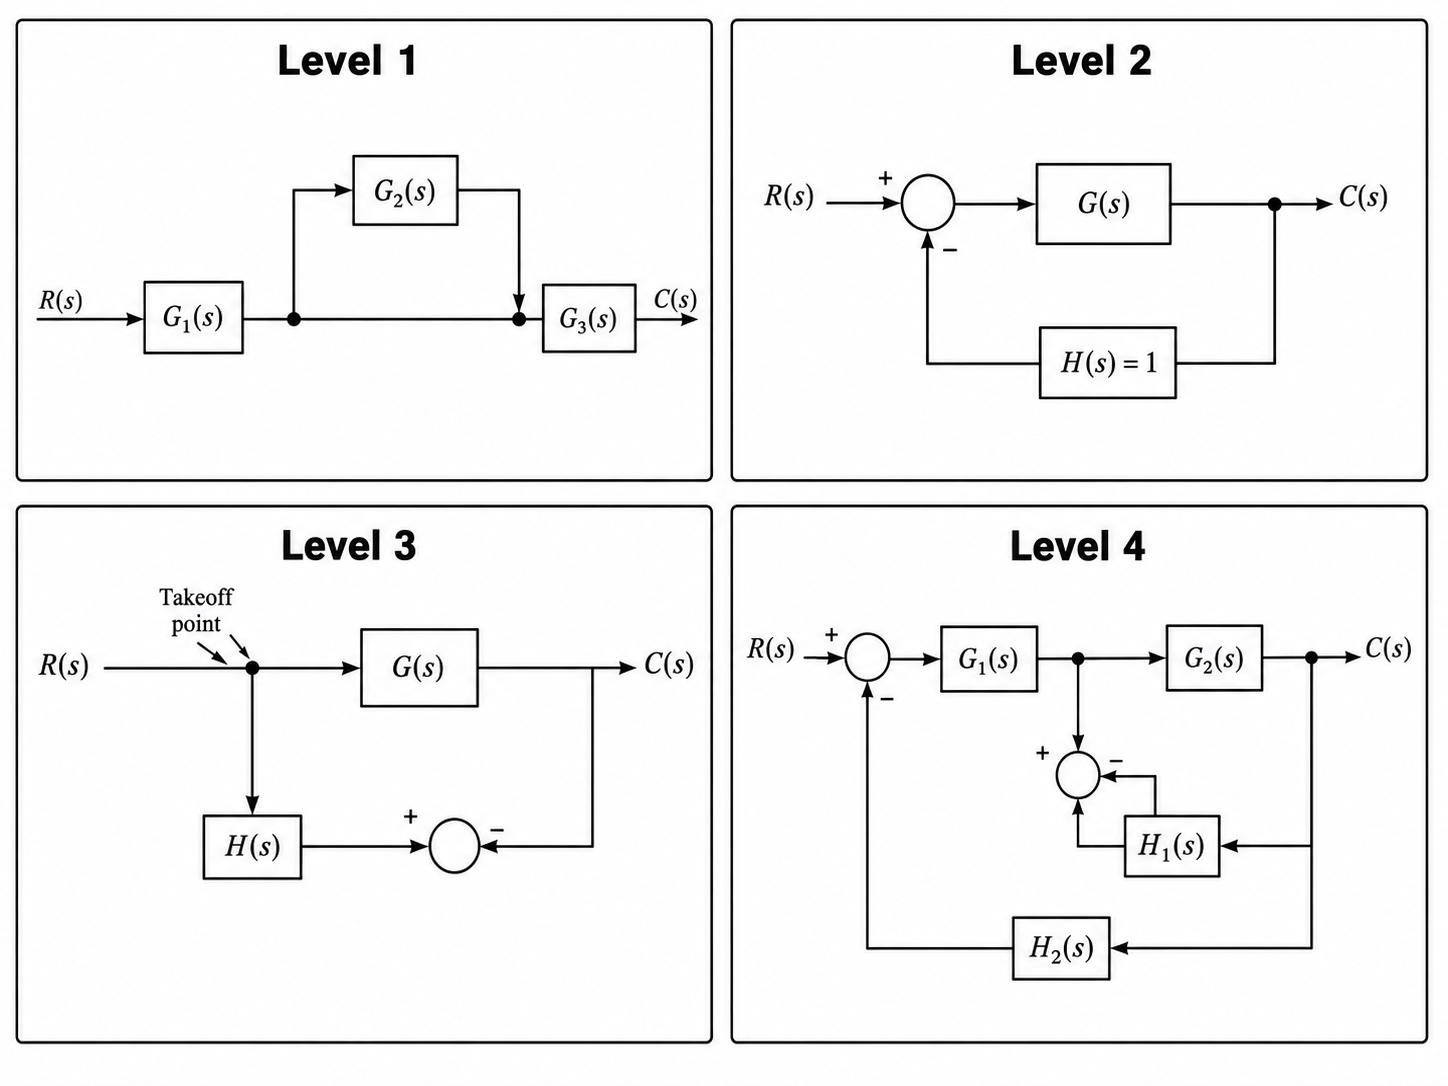
\includegraphics[width=0.8\textwidth]{images/chapter4/figure-08.png}
    \caption{ชุดแผนภาพบล็อกฝึกปฏิบัติ 4 ระดับความยากสำหรับกิจกรรมปฏิบัติการที่ 1}
\end{figure}

\textbf{5. ข้อควรระวังด้านความปลอดภัย:} กิจกรรมนี้เป็นการคำนวณบนกระดาษ ไม่มีความเสี่ยงทางกายภาพ ควรเน้นย้ำให้ผู้เรียนตรวจสอบเครื่องหมายบวกลบและลำดับขั้นตอนอย่างรอบคอบเพื่อป้องกันข้อผิดพลาดทางคณิตศาสตร์

\textbf{6. ขั้นตอนการปฏิบัติ:}
\begin{enumerate}
    \item รับใบงานแผนภาพบล็อกทั้ง 4 ระดับ
    \item วิเคราะห์โครงสร้างและระบุว่าต้องใช้กฎใดบ้างในแต่ละระดับ
    \item ลดรูปทีละขั้นตอน โดยเขียนแสดงทุกขั้นตอนอย่างชัดเจน (ห้ามข้ามขั้นตอน)
    \item เปรียบเทียบคำตอบกับเพื่อนในกลุ่ม (ทำงานเป็นคู่)
    \item ส่งใบงานให้ผู้สอนตรวจสอบ
\end{enumerate}

\textbf{7. ตารางบันทึกผล}

\textbf{ตารางที่ 5} บันทึกผลการลดรูปแผนภาพบล็อกทั้ง 4 ระดับ

\begin{table}[htbp]
    \centering
    \begin{tabular}{l l l l l}
        \hline
        \textbf{ระดับ} & \textbf{กฎที่ใช้ (เรียงลำดับ)} & \textbf{จำนวนขั้นตอน} & \textbf{Transfer Function ที่ได้} & \textbf{ตรวจสอบกับเฉลยแล้ว ($\checkmark$/$\times$)} \\
        \hline
        1 &  &  &  &  \\
        2 &  &  &  &  \\
        3 &  &  &  &  \\
        4 &  &  &  &  \\
        \hline
    \end{tabular}
\end{table}

\textbf{8. การคำนวณและวิเคราะห์ผล:} เปรียบเทียบจำนวนขั้นตอนที่ใช้ในแต่ละระดับ และระบุว่าขั้นตอนใดใช้เวลานานที่สุดหรือเสี่ยงต่อความผิดพลาดมากที่สุด

\textbf{9. การเปรียบเทียบผลกับเฉลย:} ตรวจคำตอบกับเฉลยที่ผู้สอนเตรียมไว้ (ดูหัวข้อ 14 เฉลยแบบฝึกหัด) หากไม่ตรงกัน ให้ย้อนกลับไปตรวจแต่ละขั้นตอน

\textbf{10. คำถามหลังการทดลอง:}
\begin{itemize}
    \item ระดับใดที่ใช้เวลานานที่สุด เพราะเหตุใด
    \item ขั้นตอนการเลื่อนจุดแยกสัญญาณในระดับที่ 3 ทำให้เกิดบล็อกเพิ่มเติมใด และเพราะเหตุใดจึงจำเป็น
    \item ในระดับที่ 4 เหตุใดจึงต้องลดรูปลูปในสุดก่อนลูปนอกสุดเสมอ
\end{itemize}

\textbf{11. เกณฑ์การประเมิน:} ความถูกต้องของ transfer function ที่ได้ในแต่ละระดับ ความครบถ้วนของขั้นตอนที่แสดง และความสามารถในการอธิบายเหตุผลของแต่ละขั้นตอน

\subsubsection{กิจกรรมปฏิบัติการที่ 2: ยืนยันผลด้วยคำสั่ง MATLAB}

\textbf{1. วัตถุประสงค์:} ผู้เรียนสามารถใช้คำสั่ง \texttt{series()}, \texttt{parallel()}, \texttt{feedback()} ใน MATLAB เพื่อยืนยันผลการลดรูปที่คำนวณด้วยมือในกิจกรรมปฏิบัติการที่ 1

\textbf{2. หลักการและทฤษฎีที่เกี่ยวข้อง:} การนิยาม transfer function ด้วย \texttt{tf()} และคำสั่งกลุ่มลดรูปแผนภาพบล็อกใน Control System Toolbox (หัวข้อ 7.8)

\textbf{3. อุปกรณ์ เครื่องมือ และซอฟต์แวร์:} เครื่องคอมพิวเตอร์ที่ติดตั้ง MATLAB พร้อม Control System Toolbox

\textbf{4. แผนภาพหรือวงจร:} ใช้โครงสร้างแผนภาพบล็อกเดียวกันกับกิจกรรมปฏิบัติการที่ 1 ทั้ง 4 ระดับ

\textbf{5. ข้อควรระวังด้านความปลอดภัย:} ไม่มีความเสี่ยงทางกายภาพ ควรตรวจสอบสิทธิ์การใช้งาน MATLAB และ Toolbox ที่จำเป็นก่อนเริ่มกิจกรรม

\textbf{6. ขั้นตอนการปฏิบัติ:}
\begin{enumerate}
    \item เปิด MATLAB และสร้างสคริปต์ใหม่
    \item นิยาม transfer function ของแต่ละบล็อกด้วย \texttt{tf()} ตามใบงาน
    \item ใช้คำสั่ง \texttt{series}, \texttt{parallel}, \texttt{feedback} ตามลำดับโครงสร้างของแต่ละระดับ
    \item แสดงผลลัพธ์ด้วย \texttt{disp()} หรือกราฟการตอบสนองด้วย \texttt{step()}
    \item บันทึกผลลัพธ์และเปรียบเทียบกับคำตอบที่คำนวณด้วยมือ
\end{enumerate}

\textbf{7. ตารางบันทึกผล}

\textbf{ตารางที่ 6} เปรียบเทียบผลจากการคำนวณด้วยมือกับ MATLAB

\begin{table}[htbp]
    \centering
    \small
    \begin{tabularx}{\textwidth}{L{0.10\textwidth} Y Y L{0.18\textwidth}}
        \hline
        \textbf{ระดับ} & \textbf{Transfer Function จากการคำนวณด้วยมือ} & \textbf{Transfer Function จาก MATLAB} & \textbf{ตรงกันหรือไม่ ($\checkmark$/$\times$)} \\
        \hline
        1 &  &  &  \\
        2 &  &  &  \\
        3 &  &  &  \\
        4 &  &  &  \\
        \hline
    \end{tabularx}
\end{table}

\textbf{8. การคำนวณและวิเคราะห์ผล:} ตรวจสอบว่าค่าสัมประสิทธิ์ของพหุนามเศษและส่วนตรงกันหรือไม่ หากไม่ตรงกันให้ระบุจุดที่ผิดพลาด

\textbf{9. การเปรียบเทียบผลกับทฤษฎี:} ผลจาก MATLAB ต้องตรงกับผลการคำนวณด้วยมือทุกระดับ หากไม่ตรงกันให้ตรวจสอบทั้งสองฝั่ง

\textbf{10. คำถามหลังการทดลอง:} คำสั่งใดของ MATLAB ที่ช่วยลดขั้นตอนได้มากที่สุดเมื่อเทียบกับการคำนวณด้วยมือ และเพราะเหตุใด

\textbf{11. เกณฑ์การประเมิน:} ความถูกต้องของสคริปต์ ความตรงกันของผลลัพธ์กับการคำนวณด้วยมือ และการบันทึกเปรียบเทียบอย่างเป็นระบบ

\subsubsection{กิจกรรมปฏิบัติการที่ 3: ยืนยันผลด้วย Simulink}

\textbf{1. วัตถุประสงค์:} ผู้เรียนสามารถสร้างแบบจำลอง Simulink ของระบบเดิม (ไม่ลดรูป) และเปรียบเทียบสัญญาณเอาต์พุตกับแบบจำลองที่ใช้ transfer function รวมที่ลดรูปแล้ว

\textbf{2. หลักการและทฤษฎีที่เกี่ยวข้อง:} การใช้บล็อก Transfer Fcn, Step และ Scope ใน Simulink (หัวข้อ 7.8)

\textbf{3. อุปกรณ์ เครื่องมือ และซอฟต์แวร์:} เครื่องคอมพิวเตอร์ที่ติดตั้ง MATLAB/Simulink

\textbf{4. แผนภาพหรือวงจร:} ใช้ระดับที่ 2 และระดับที่ 4 จากกิจกรรมปฏิบัติการที่ 1 เป็นกรณีศึกษา เนื่องจากมีลูปป้อนกลับที่ชัดเจน

% [รูปที่ 9: ตัวอย่างการจัดวางบล็อกใน Simulink สำหรับยืนยันผลการลดรูป]
% ประเภทภาพ: Experimental Setup
% ตำแหน่งที่แนะนำ: ในกิจกรรมปฏิบัติการที่ 3 หัวข้อที่ 4
% วัตถุประสงค์การเรียนรู้: ให้ผู้เรียนเห็นตัวอย่างการจัดวางบล็อก Simulink ก่อนเริ่มสร้างแบบจำลองจริง
% คำอธิบายภาพ: แสดงบล็อก Step เชื่อมเข้าบล็อก Transfer Fcn สองบล็อกต่ออนุกรมกันในลูปป้อนกลับ ต่อไปยังบล็อก Scope โดยมีจุดแยกสัญญาณย้อนกลับผ่านบล็อกป้อนกลับ Gain เข้าสู่บล็อก Sum ก่อนเข้า Transfer Fcn ตัวแรก จัดวางในลักษณะหน้าต่างแบบจำลอง Simulink
% องค์ประกอบที่ต้องมี: บล็อก Step, Sum, Transfer Fcn (สองบล็อก), Gain (ป้อนกลับ), Scope, เส้นเชื่อมสัญญาณ
% ข้อความหรือป้ายกำกับ: "Step", "Transfer Fcn", "Gain", "Scope", "Sum"
% ภาษาของป้ายกำกับ: อังกฤษ
% สัดส่วนภาพ: 16:9
% Image Generation Prompt: A Simulink model window diagram showing a Step input block connected to a Sum block, then to two Transfer Fcn blocks in series, output going to a Scope block, with a feedback branch through a Gain block returning to the Sum block. Style resembles a simplified Simulink canvas with light gray block outlines and blue signal lines on white background, block labels in clear sans-serif font.
% Alt Text: ภาพตัวอย่างการจัดวางบล็อกในแบบจำลอง Simulink สำหรับยืนยันผลการลดรูปแผนภาพบล็อก

\begin{figure}[htbp]
    \centering
    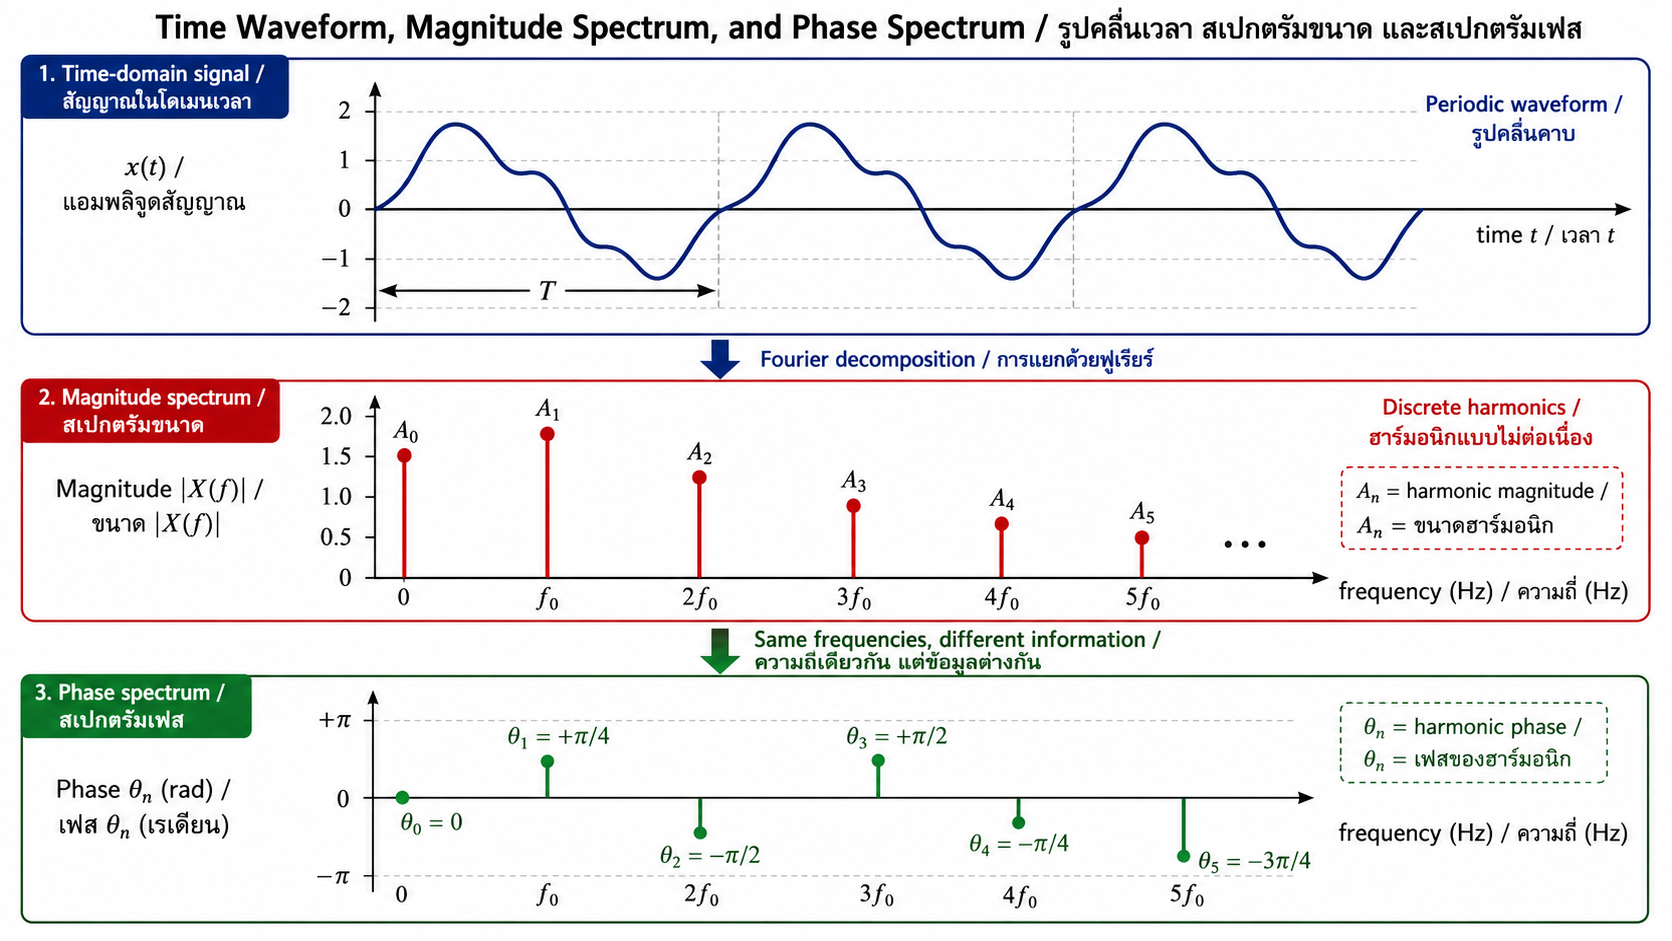
\includegraphics[width=0.8\textwidth]{images/chapter4/figure-09.png}
    \caption{ตัวอย่างการจัดวางบล็อกใน Simulink สำหรับยืนยันผลการลดรูป}
\end{figure}

\textbf{5. ข้อควรระวังด้านความปลอดภัย:} ไม่มีความเสี่ยงทางกายภาพ ควรตั้งค่าเวลาจำลอง (simulation time) และ step size ให้เหมาะสมเพื่อให้ Scope แสดงผลครบช่วงเวลาที่สนใจ

\textbf{6. ขั้นตอนการปฏิบัติ:}
\begin{enumerate}
    \item เปิด Simulink และสร้างแบบจำลองใหม่
    \item วางบล็อก Transfer Fcn ตามโครงสร้างเดิมของระบบ (ไม่ลดรูป) พร้อมบล็อก Sum และ Gain ตามที่จำเป็น
    \item ต่อบล็อก Step เป็นสัญญาณอินพุตและบล็อก Scope ที่เอาต์พุต
    \item รันการจำลองและบันทึกรูปคลื่น
    \item สร้างแบบจำลองที่สองโดยใช้บล็อก Transfer Fcn เพียงตัวเดียวที่มีค่าเท่ากับ transfer function รวมที่ลดรูปแล้ว
    \item เปรียบเทียบรูปคลื่นจากทั้งสอง Scope
\end{enumerate}

\textbf{7. ตารางบันทึกผล}

\textbf{ตารางที่ 7} เปรียบเทียบผลตอบสนองจากแบบจำลอง Simulink ทั้งสองแบบ

\begin{table}[htbp]
    \centering
    \small
    \begin{tabularx}{\textwidth}{L{0.24\textwidth} Y Y L{0.18\textwidth}}
        \hline
        \textbf{กรณี} & \textbf{ค่า Steady-State ที่อ่านได้} & \textbf{เวลาที่เข้าสู่ค่าคงตัวโดยประมาณ (วินาที)} & \textbf{รูปคลื่นซ้อนทับกันหรือไม่ ($\checkmark$/$\times$)} \\
        \hline
        ระดับ 2 (โมเดลไม่ลดรูป) &  &  &  \\
        ระดับ 2 (โมเดลลดรูปแล้ว) &  &  &  \\
        ระดับ 4 (โมเดลไม่ลดรูป) &  &  &  \\
        ระดับ 4 (โมเดลลดรูปแล้ว) &  &  &  \\
        \hline
    \end{tabularx}
\end{table}

\textbf{8. การคำนวณและวิเคราะห์ผล:} หากรูปคลื่นของสองแบบจำลองไม่ซ้อนทับกัน ให้ตรวจสอบพารามิเตอร์บล็อกและเครื่องหมายของสัญญาณป้อนกลับ

\textbf{9. การเปรียบเทียบผลกับทฤษฎี:} ผลจาก Simulink ต้องสอดคล้องกับผลจาก MATLAB ในกิจกรรมปฏิบัติการที่ 2 และผลคำนวณด้วยมือในกิจกรรมปฏิบัติการที่ 1

\textbf{10. คำถามหลังการทดลอง:} เพราะเหตุใดสัญญาณเอาต์พุตของสองแบบจำลองจึงต้องซ้อนทับกันพอดีหากการลดรูปถูกต้อง และหากไม่ซ้อนทับกันควรเริ่มตรวจสอบจากจุดใดก่อน

\textbf{11. เกณฑ์การประเมิน:} ความถูกต้องของการสร้างแบบจำลอง Simulink ความสอดคล้องของผลลัพธ์ระหว่างสองแบบจำลอง และคุณภาพของการวิเคราะห์เมื่อพบความคลาดเคลื่อน

\subsubsection{กิจกรรมปฏิบัติการที่ 4: สร้างตารางช่วยคำนวณ Mason's Gain Formula}

\textbf{1. วัตถุประสงค์:} ผู้เรียนสามารถจัดระบบการคำนวณ Mason's Gain Formula ด้วยตารางช่วยคำนวณที่ครอบคลุม $P_k$, Loop gain, คู่ลูปไม่สัมผัสกัน, $\Delta$ และ $\Delta_k$ เพื่อลดข้อผิดพลาดจากการคำนวณอย่างไม่เป็นระบบ

\textbf{2. หลักการและทฤษฎีที่เกี่ยวข้อง:} Signal Flow Graph และ Mason's Gain Formula (หัวข้อ 7.5–7.6)

\textbf{3. อุปกรณ์ เครื่องมือ และซอฟต์แวร์:} กระดาษ หรือโปรแกรมตารางคำนวณ (เช่น Excel) สำหรับสร้างตาราง

\textbf{4. แผนภาพหรือวงจร:} ใช้ Signal Flow Graph จากตัวอย่างที่ 4 (รูปที่ 7) เป็นกรณีฝึกครั้งแรก จากนั้นผู้สอนอาจเตรียม SFG เพิ่มเติมอีก 1–2 แบบที่มีความซับซ้อนต่างกันสำหรับฝึกเพิ่มเติม

\textbf{5. ข้อควรระวังด้านความปลอดภัย:} ไม่มีความเสี่ยงทางกายภาพ ควรเน้นย้ำการตรวจทานการระบุลูปที่ไม่สัมผัสกันอย่างรอบคอบ เนื่องจากเป็นจุดที่เกิดข้อผิดพลาดบ่อยที่สุด

\textbf{6. ขั้นตอนการปฏิบัติ:}
\begin{enumerate}
    \item รับใบงาน Signal Flow Graph
    \item ระบุเส้นทางหน้าทั้งหมดและกรอกอัตราขยาย $P_k$ ลงในตาราง
    \item ระบุลูปทั้งหมดในกราฟและกรอกอัตราขยายลูปลงในตาราง
    \item ตรวจสอบและกรอกคู่ (หรือกลุ่ม) ของลูปที่ไม่สัมผัสกัน
    \item คำนวณ $\Delta$ จากผลรวมและผลคูณตามสูตร
    \item คำนวณ $\Delta_k$ ของแต่ละเส้นทางหน้า โดยตัดลูปที่สัมผัสกับเส้นทางนั้นออก
    \item แทนค่าในสูตรเมสันเพื่อสรุปผล $C(s)/R(s)$
\end{enumerate}

\textbf{7. ตารางบันทึกผล (Template)}

\textbf{ตารางที่ 8} Template ตารางช่วยคำนวณ Mason's Gain Formula

\begin{table}[htbp]
    \centering
    \begin{tabular}{l l l l l}
        \hline
        \textbf{เส้นทางหน้า/ลูป} & \textbf{โหนดที่ผ่าน} & \textbf{อัตราขยาย ($P_k$ หรือ Loop Gain)} & \textbf{สัมผัสกับลูปใดบ้าง} & \textbf{หมายเหตุ} \\
        \hline
        $P_1$ &  &  &  &  \\
        $P_2$ &  &  &  &  \\
        $L_1$ &  &  &  &  \\
        $L_2$ &  &  &  &  \\
        \hline
    \end{tabular}
\end{table}

\begin{table}[htbp]
    \centering
    \begin{tabular}{l l}
        \hline
        \textbf{คู่ลูปไม่สัมผัสกัน} & \textbf{ผลคูณอัตราขยาย} \\
        \hline
         &  \\
        \hline
    \end{tabular}
\end{table}

\begin{table}[htbp]
    \centering
    \begin{tabular}{l l l}
        \hline
        \textbf{รายการ} & \textbf{สูตร} & \textbf{ค่าที่คำนวณได้} \\
        \hline
        $\Delta$ & $1-\sum L_i+\sum L_iL_j-\cdots$ &  \\
        $\Delta_1$ &  &  \\
        $\Delta_2$ &  &  \\
        $C(s)/R(s)$ & $\dfrac{1}{\Delta}\sum P_k\Delta_k$ &  \\
        \hline
    \end{tabular}
\end{table}

\textbf{8. การคำนวณและวิเคราะห์ผล:} ใช้ตัวอย่างที่ 4 เป็นกรณีอ้างอิงตรวจสอบความถูกต้องของตารางก่อนนำไปใช้กับ SFG ชุดใหม่

\textbf{9. การเปรียบเทียบผลกับเฉลย:} ตรวจคำตอบกับเฉลยที่ผู้สอนเตรียมไว้

\textbf{10. คำถามหลังการทดลอง:} การใช้ตารางช่วยลดข้อผิดพลาดในขั้นตอนใดได้ชัดเจนที่สุดเมื่อเทียบกับการคำนวณอย่างอิสระโดยไม่มีตาราง

\textbf{11. เกณฑ์การประเมิน:} ความครบถ้วนของตาราง ความถูกต้องของ $\Delta$ และ $\Delta_k$ และความถูกต้องของผลลัพธ์สุดท้าย


\subsection{11. สรุปท้ายบท}

Block Diagram เป็นเครื่องมือแสดงความสัมพันธ์เชิงฟังก์ชันของระบบควบคุมด้วยบล็อก จุดรวมสัญญาณ และจุดแยกสัญญาณ ภายใต้สมมติฐานว่าสัญญาณไหลทิศทางเดียวและไม่มีผลโหลดต่อกัน การลดรูปแผนภาพบล็อกอาศัยกฎหลัก 3 กฎ คือ การต่อแบบอนุกรม ($G_1G_2$) การต่อแบบขนาน ($G_1\pm G_2$) และการป้อนกลับ ($G/(1\pm GH)$) ร่วมกับกฎเสริมสำหรับเลื่อนจุดรวมสัญญาณและจุดแยกสัญญาณเมื่อกฎหลักใช้ไม่ได้โดยตรง โดยควรลดรูปลูปในสุดก่อนเสมอเมื่อระบบมีหลายลูปซ้อนกัน

Signal Flow Graph เป็นอีกแนวทางหนึ่งที่แทนความสัมพันธ์เชิงเส้นด้วยโหนดและกิ่ง และใช้ \textbf{Mason's Gain Formula} คำนวณ transfer function รวมได้โดยตรงจากโครงสร้างกราฟ

\[
P = \frac{1}{\Delta}\sum_k P_k\Delta_k, \qquad \Delta = 1-\sum L_i+\sum L_iL_j-\cdots
\]

โดยจุดสำคัญที่สุดคือการระบุ\textbf{ลูปที่ไม่สัมผัสกัน (non-touching loop)} ให้ครบถ้วนทั้งในการคำนวณ $\Delta$ และโคแฟกเตอร์ $\Delta_k$ ของแต่ละเส้นทางหน้า ทั้งสองวิธีให้ผลลัพธ์ transfer function เดียวกันเสมอเมื่อคำนวณถูกต้อง โดย Block Diagram Reduction เหมาะกับระบบที่มีลูปไม่มากและไม่ซ้อนกันซับซ้อน ในขณะที่ Signal Flow Graph กับ Mason's Gain Formula เหมาะกับระบบที่มีหลายลูปซ้อนกันหรือมีหลายเส้นทางหน้า ผลลัพธ์ที่ได้จากทั้งสองวิธีสามารถยืนยันได้ด้วยคำสั่ง MATLAB (\texttt{series}, \texttt{parallel}, \texttt{feedback}) และแบบจำลอง Simulink

\par\noindent\rule{\textwidth}{0.4pt}\par

\subsection{12. คำถามทบทวน}

\begin{enumerate}
    \item Block Diagram ในระบบควบคุมประกอบด้วยองค์ประกอบพื้นฐานใดบ้าง และแต่ละองค์ประกอบทำหน้าที่อย่างไร
    \item เพราะเหตุใดการต่อแบบอนุกรมจึงใช้การคูณ transfer function ในขณะที่การต่อแบบขนานใช้การบวก
    \item จงเขียนสูตร closed-loop transfer function สำหรับระบบป้อนกลับเชิงลบและเชิงบวก พร้อมอธิบายความแตกต่างของเครื่องหมาย
    \item การเลื่อนจุดรวมสัญญาณไปด้านหน้าบล็อกกับด้านหลังบล็อกต้องเพิ่มบล็อกชดเชยต่างกันอย่างไร เพราะเหตุใด
    \item จงอธิบายความแตกต่างระหว่าง Path, Forward Path และ Loop ใน Signal Flow Graph
    \item Non-touching Loop คืออะไร และเหตุใดจึงมีความสำคัญต่อการคำนวณด้วย Mason's Gain Formula
    \item จงเขียน Mason's Gain Formula พร้อมอธิบายความหมายของสัญลักษณ์ $P_k$, $\Delta$ และ $\Delta_k$ ในสูตร
    \item เพราะเหตุใดโคแฟกเตอร์ $\Delta_k$ ของแต่ละเส้นทางหน้าจึงอาจมีค่าไม่เท่ากัน ยกตัวอย่างประกอบ
    \item จงเปรียบเทียบข้อดีและข้อจำกัดของการลดรูปแผนภาพบล็อกกับการใช้ Signal Flow Graph ร่วมกับ Mason's Gain Formula
    \item คำสั่ง MATLAB ใดใช้สำหรับยืนยันผลการต่อแบบอนุกรม ขนาน และป้อนกลับตามลำดับ และแต่ละคำสั่งคำนวณตามสูตรใด
\end{enumerate}

\newpage

\subsection{13. แบบฝึกหัดท้ายบท}

\textit{หมายเหตุ: โจทย์ทั้งหมดในหัวข้อนี้สร้างขึ้นให้สอดคล้องกับเนื้อหาที่อธิบายในบท เฉลยแยกไว้ในหัวข้อ 14 สำหรับผู้สอน}

\subsubsection{ระดับพื้นฐาน}

\textbf{ข้อ 1.} ระบบมีบล็อก $G_1(s)=\dfrac{4}{s+1}$ และ $G_2(s)=\dfrac{2}{s+3}$ ต่อกันแบบอนุกรม จงหา transfer function รวม

\textbf{ข้อ 2.} ระบบมีบล็อก $G_1(s)=\dfrac{5}{s+2}$ และ $G_2(s)=\dfrac{3}{s+4}$ ต่อกันแบบขนานโดยสัญญาณรวมกันด้วยเครื่องหมายบวก จงหา transfer function รวม

\textbf{ข้อ 3.} ระบบป้อนกลับหนึ่งหน่วยเชิงลบมี $G(s)=\dfrac{6}{s+1}$ จงหา closed-loop transfer function

\textbf{ข้อ 4.} จงระบุว่า Signal Flow Graph ที่มีโหนด $R \to 1 \to 2 \to C$ (ไม่มีลูปย้อนกลับ) มีเส้นทางหน้ากี่เส้นทาง และมีลูปหรือไม่

\textbf{ข้อ 5.} จงอธิบายความแตกต่างระหว่างจุดรวมสัญญาณและจุดแยกสัญญาณ พร้อมยกตัวอย่างระบบที่พบทั้งสององค์ประกอบ

\subsubsection{ระดับวิเคราะห์}

\textbf{ข้อ 6.} ระบบมีเส้นทางไปข้างหน้า $G(s)=\dfrac{8}{s(s+3)}$ และป้อนกลับเชิงลบผ่าน $H(s)=0.5$ จงหา closed-loop transfer function และระบุตำแหน่งขั้ว (pole)

\textbf{ข้อ 7.} แผนภาพบล็อกมี $G_1(s)=\dfrac{2}{s+1}$ ต่ออนุกรมกับ $G_2(s)=\dfrac{3}{s+2}$ แล้วผลลัพธ์รวมมีลูปป้อนกลับเชิงลบผ่าน $H(s)=1$ จงลดรูปเป็น transfer function เดียว

\textbf{ข้อ 8.} Signal Flow Graph มีเส้นทางหน้าเดียว $P_1 = G_1G_2G_3$ และลูปสองลูปที่\textbf{สัมผัสกัน} (มีโหนดร่วม) คือ $L_1$ และ $L_2$ จงเขียนสูตรคำนวณ $\Delta$ ของกราฟนี้ พร้อมอธิบายว่าเหตุใดจึงไม่มีพจน์ $L_1L_2$ ในสูตร

\textbf{ข้อ 9.} จงเปรียบเทียบจำนวนขั้นตอนที่ต้องใช้ในการหา transfer function ของระบบที่มี 3 ลูปป้อนกลับซ้อนกัน ระหว่างวิธีลดรูปแผนภาพบล็อกกับวิธี Mason's Gain Formula

\textbf{ข้อ 10.} ระบบมีจุดแยกสัญญาณอยู่ก่อนบล็อก $G(s)=\dfrac{1}{s+5}$ และจำเป็นต้องเลื่อนจุดแยกสัญญาณไปด้านหลังบล็อกเพื่อรวมกับบล็อกอื่น จงระบุบล็อกชดเชยที่ต้องเพิ่มในเส้นสัญญาณที่แยกออกไป

\subsubsection{ระดับประยุกต์ใช้}

\textbf{ข้อ 11.} ระบบควบคุมความเร็วมอเตอร์มีตัวควบคุม $G_c(s)=\dfrac{K}{s}$ (โดย $K=4$) ต่ออนุกรมกับมอเตอร์ $G_m(s)=\dfrac{2}{s+5}$ และมีเซนเซอร์ป้อนกลับ $H(s)=0.1$ จงหา closed-loop transfer function ของระบบทั้งหมด และยืนยันผลด้วยคำสั่ง MATLAB \texttt{series} และ \texttt{feedback}

\textbf{ข้อ 12.} ระบบควบคุมท่าทางมีลูปในควบคุมอัตราการหมุน (inner loop) และลูปนอกควบคุมมุม (outer loop) ซ้อนกัน จงอธิบายว่าเหตุใดวิศวกรจึงมักเลือกใช้ Signal Flow Graph แทนการลดรูปแผนภาพบล็อกทีละขั้นตอนสำหรับระบบลักษณะนี้ พร้อมยกเหตุผลสนับสนุนอย่างน้อย 2 ข้อ

\textbf{ข้อ 13.} จงสร้าง Signal Flow Graph ของระบบที่มีสองเส้นทางหน้าและสองลูปที่\textbf{ไม่สัมผัสกัน} ขึ้นเองหนึ่งชุด (กำหนดอัตราขยายเป็นสัญลักษณ์ได้) แล้วคำนวณ transfer function รวมด้วย Mason's Gain Formula พร้อมแสดงตารางช่วยคำนวณตามรูปแบบในหัวข้อกิจกรรมปฏิบัติการที่ 4

\par\noindent\rule{\textwidth}{0.4pt}\par

\newpage

\subsection{14. เฉลยแบบฝึกหัด (สำหรับผู้สอน)}

\textit{หมายเหตุ: หัวข้อนี้จัดทำสำหรับผู้สอนใช้ตรวจสอบคำตอบ หากต้องการจัดทำเอกสารสำหรับนักศึกษาโดยไม่เปิดเผยคำตอบ ให้แยกหัวข้อนี้ออกเป็นไฟล์ต่างหาก}

\subsubsection{เฉลยระดับพื้นฐาน}

\textbf{ข้อ 1.} ใช้กฎการต่อแบบอนุกรม:
\[
G_{eq}(s)=G_1(s)G_2(s)=\dfrac{4}{s+1}\cdot\dfrac{2}{s+3}
=\dfrac{8}{(s+1)(s+3)}=\dfrac{8}{s^2+4s+3}
\]
คำตอบ: $\dfrac{8}{s^2+4s+3}$ ข้อผิดพลาดที่พบบ่อย: นักศึกษามักบวกแทนที่จะคูณ

\textbf{ข้อ 2.} ใช้กฎการต่อแบบขนาน: $G_{eq}(s)=\dfrac{5}{s+2}+\dfrac{3}{s+4}=\dfrac{5(s+4)+3(s+2)}{(s+2)(s+4)}=\dfrac{8s+26}{s^2+6s+8}$ — คำตอบ: $\dfrac{8s+26}{s^2+6s+8}$

\textbf{ข้อ 3.} ใช้สูตรป้อนกลับเชิงลบ: $\dfrac{C(s)}{R(s)}=\dfrac{G(s)}{1+G(s)}=\dfrac{6/(s+1)}{1+6/(s+1)}=\dfrac{6}{s+7}$ — คำตอบ: $\dfrac{6}{s+7}$ การแปลความหมาย: ขั้วเลื่อนจาก $s=-1$ (open-loop) ไปที่ $s=-7$ (closed-loop) แสดงว่าระบบตอบสนองเร็วขึ้นเมื่อปิดลูป

\textbf{ข้อ 4.} มีเส้นทางหน้าเพียง 1 เส้นทาง ($R\to1\to2\to C$) และ\textbf{ไม่มีลูป}เนื่องจากไม่มีกิ่งใดย้อนกลับไปยังโหนดที่ผ่านมาแล้ว

\textbf{ข้อ 5.} จุดรวมสัญญาณรวมสัญญาณตั้งแต่สองสัญญาณขึ้นไปด้วยการบวกหรือลบ (เช่น จุดเปรียบเทียบค่าอ้างอิงกับสัญญาณป้อนกลับ) ส่วนจุดแยกสัญญาณแยกสัญญาณเดียวส่งไปหลายเส้นทางโดยไม่เปลี่ยนค่า (เช่น จุดที่ส่งสัญญาณเอาต์พุตไปทั้งโหลดและกลับไปยังเซนเซอร์ป้อนกลับพร้อมกัน)

\subsubsection{เฉลยระดับวิเคราะห์}

\textbf{ข้อ 6.} $\dfrac{C(s)}{R(s)}=\dfrac{G(s)}{1+G(s)H(s)}=\dfrac{8/[s(s+3)]}{1+0.5\cdot8/[s(s+3)]}=\dfrac{8}{s(s+3)+4}=\dfrac{8}{s^2+3s+4}$ ขั้วอยู่ที่รากของ $s^2+3s+4=0$ คือ $s=\dfrac{-3\pm\sqrt{9-16}}{2}=-1.5\pm j1.32$ (ขั้วเชิงซ้อนคู่ควบ)

\textbf{ข้อ 7.} ลดรูปอนุกรมก่อน: $G_1G_2=\dfrac{2}{s+1}\cdot\dfrac{3}{s+2}=\dfrac{6}{(s+1)(s+2)}$ จากนั้นปิดลูปป้อนกลับหนึ่งหน่วยเชิงลบ: $\dfrac{6/[(s+1)(s+2)]}{1+6/[(s+1)(s+2)]}=\dfrac{6}{(s+1)(s+2)+6}=\dfrac{6}{s^2+3s+8}$

\textbf{ข้อ 8.} $\Delta = 1-(L_1+L_2)$ เนื่องจาก $L_1$ และ $L_2$ สัมผัสกัน (มีโหนดร่วม) จึงไม่มีคู่ลูปไม่สัมผัสกันให้พิจารณา พจน์ $L_1L_2$ (ผลคูณของคู่ลูปไม่สัมผัสกัน) จึงไม่ปรากฏในสูตร

\textbf{ข้อ 9.} วิธีลดรูปแผนภาพบล็อกต้องเลื่อนจุดรวม/จุดแยกสัญญาณและลดรูปทีละลูปจากในสุดไปนอกสุด ใช้หลายขั้นตอนและเสี่ยงต่อความผิดพลาดสะสม ส่วนวิธี Mason's Gain Formula คำนวณ $\Delta$ และ $\Delta_k$ จากโครงสร้างกราฟได้โดยตรงในขั้นตอนเดียว จึงมักใช้ขั้นตอนน้อยกว่าเมื่อระบบมีลูปซ้อนกันหลายชั้น แต่ต้องระบุลูปไม่สัมผัสกันให้ครบถ้วน

\textbf{ข้อ 10.} ต้องเพิ่มบล็อก $1/G(s) = (s+5)$ เข้าที่เส้นสัญญาณที่แยกออกไป เพื่อให้ค่าสัญญาณที่จุดแยกเดิมไม่เปลี่ยนแปลงหลังเลื่อนตำแหน่ง

\subsubsection{เฉลยระดับประยุกต์ใช้}

\textbf{ข้อ 11.} ลดรูปอนุกรมก่อน: $G_c(s)G_m(s)=\dfrac{4}{s}\cdot\dfrac{2}{s+5}=\dfrac{8}{s(s+5)}=\dfrac{8}{s^2+5s}$ จากนั้นปิดลูปป้อนกลับ: $\dfrac{C(s)}{R(s)}=\dfrac{8/(s^2+5s)}{1+0.1\cdot8/(s^2+5s)}=\dfrac{8}{s^2+5s+0.8}$ ตรวจสอบด้วย MATLAB: \texttt{G = series(tf([4],[1 0]), tf([2],[1 5])); Gcl = feedback(G, 0.1);} ผลลัพธ์ที่ได้ต้องมีสัมประสิทธิ์ตรงกับที่คำนวณด้วยมือ

\textbf{ข้อ 12.} เหตุผลสนับสนุน ได้แก่ (1) ระบบมีลูปซ้อนกันตั้งแต่สองชั้นขึ้นไป การลดรูปแผนภาพบล็อกทีละขั้นตอนต้องเลื่อนจุดรวม/จุดแยกสัญญาณหลายครั้งและเสี่ยงต่อข้อผิดพลาดสะสม ในขณะที่ Mason's Gain Formula คำนวณจากโครงสร้างกราฟได้โดยตรง (2) หากมีการปรับพารามิเตอร์ของลูปใดลูปหนึ่งภายหลัง (เช่น ปรับอัตราขยายตัวควบคุม) การคำนวณใหม่ด้วย SFG ทำได้รวดเร็วกว่าเพราะไม่ต้องไล่ลดรูปใหม่ทั้งหมด

\textbf{ข้อ 13.} คำตอบขึ้นอยู่กับ SFG ที่นักศึกษาสร้างขึ้นเอง ผู้สอนควรตรวจสอบว่า (1) มีเส้นทางหน้าสองเส้นทางจริงและไม่ผ่านโหนดซ้ำ (2) สองลูปที่ระบุไม่มีโหนดร่วมกันจริง (3) การคำนวณ $\Delta$ และ $\Delta_k$ เป็นไปตามสูตรและสอดคล้องกับตัวอย่างที่ 4 ในเนื้อหา


\subsection{15. ข้อเสนอแนะสำหรับผู้สอน}

\begin{itemize}
    \item \textbf{ลำดับการสอน:} แนะนำให้สอนกฎการลดรูปแผนภาพบล็อก (หัวข้อ 7.3) ให้แน่นก่อนจึงเข้าสู่ Signal Flow Graph และ Mason's Gain Formula เนื่องจากผู้เรียนจะเข้าใจที่มาของสูตรป้อนกลับได้ง่ายกว่าเมื่อผ่านการฝึกลดรูปด้วยกฎพีชคณิตมาก่อน
    \item \textbf{สำหรับนักศึกษาสาย ม.6:} ให้สอนการลดรูปแผนภาพบล็อกทีละขั้นตอนอย่างละเอียดก่อน โดยเน้นตัวอย่างที่ 1–3 ให้คล่องก่อนขยับไปสู่ Signal Flow Graph เพื่อไม่ให้ผู้เรียนสับสนระหว่างสองแนวคิดพร้อมกัน
    \item \textbf{สำหรับนักศึกษาสาย ปวช.:} แนะนำให้ใช้ Template ตารางคำนวณ Mason's Gain Formula (ตารางที่ 8 ในกิจกรรมปฏิบัติการที่ 4) ตั้งแต่เริ่มฝึก เพื่อลดข้อผิดพลาดจากการคำนวณอย่างไม่เป็นระบบ
    \item \textbf{จุดที่ผู้เรียนมักมีปัญหา:} การลืมบวกกลับด้วยผลคูณของคู่ลูปไม่สัมผัสกันเมื่อคำนวณ $\Delta$ และการใช้ $\Delta$ เดียวกับทุกเส้นทางหน้าโดยไม่แยกคำนวณ $\Delta_k$ ผู้สอนควรเน้นย้ำจุดนี้ด้วยตัวอย่างที่ 4 ซ้ำหลายครั้งจนผู้เรียนคล่อง
    \item \textbf{วิธีเลือกตัวอย่างเพิ่มเติม:} หากต้องการโจทย์เพิ่มเติม ควรเริ่มจากระบบที่มีเพียงหนึ่งลูปก่อน แล้วค่อยเพิ่มจำนวนลูปและเส้นทางหน้าทีละน้อย เพื่อให้ผู้เรียนเห็นพัฒนาการของความซับซ้อนอย่างเป็นลำดับ
    \item \textbf{แนวทางประเมินระหว่างเรียน:} ใช้คำถามกระตุ้นความคิดสั้น ๆ ระหว่างบรรยาย เช่น ให้ผู้เรียนระบุว่าโครงสร้างที่แสดงบนกระดานเป็นการต่อแบบใด ก่อนเฉลย เพื่อตรวจสอบความเข้าใจแบบทันที (formative assessment) และปรับจังหวะการสอนตามความเข้าใจของชั้นเรียน
\end{itemize}


\subsection{16. สื่อและแหล่งเรียนรู้เพิ่มเติม}

\begin{itemize}
    \item \textbf{NPTEL:} วิดีโอหัวข้อ Block Diagram Reduction และ Signal Flow Graph ในรายวิชา Control Systems คำค้นแนะนำ: "Block Diagram Reduction Control Systems", "Signal Flow Graph Control Systems" เหมาะสำหรับทบทวนหลังบรรยายหัวข้อ 7.3 และ 7.5
    \item \textbf{คำค้นวิดีโอ "Mason Gain Formula":} ใช้ค้นหาวิดีโอประกอบการอธิบายขั้นตอนการคำนวณ Mason's Gain Formula เหมาะสำหรับทบทวนก่อนทำกิจกรรมปฏิบัติการที่ 4
    \item \textbf{MathWorks Documentation:} เอกสารและตัวอย่าง (MATLAB examples) เกี่ยวกับคำสั่ง \texttt{feedback}, \texttt{series}, \texttt{parallel} ใน Control System Toolbox เหมาะสำหรับใช้ประกอบกิจกรรมปฏิบัติการที่ 2 โดยให้ผู้เรียนค้นหาจากเว็บไซต์ MathWorks โดยตรงเพื่อดูตัวอย่างการใช้งานฉบับล่าสุด
\end{itemize}

\textit{หมายเหตุ: รายการข้างต้นเป็นแนวทางค้นหาตามที่ผู้ใช้ระบุ ไม่มีการแต่งชื่อคลิป ลิงก์ ผู้บรรยาย หรือปีเผยแพร่ขึ้นเอง ผู้สอนควรตรวจสอบและเลือกคลิปที่เหมาะสมกับเนื้อหาก่อนนำไปใช้จริง}

\par\noindent\rule{\textwidth}{0.4pt}\par

\subsection{17. เอกสารอ้างอิง}

\textit{หมายเหตุ: รายการต่อไปนี้เป็นแหล่งอ้างอิงมาตรฐานในสาขาระบบควบคุมที่ตรงกับเนื้อหาของบทนี้ ผู้สอนควรตรวจสอบรายละเอียดฉบับพิมพ์ (edition, ปีพิมพ์, สำนักพิมพ์) ให้ตรงกับฉบับที่ใช้อ้างอิงจริงก่อนเผยแพร่}

\begin{enumerate}
    \item Ogata, K. (2010). \textit{Modern Control Engineering} (5th ed.). Prentice Hall. — บทที่ว่าด้วย Block Diagrams และ Signal Flow Graphs
    \item Nise, N. S. (2015). \textit{Control Systems Engineering} (7th ed.). Wiley. — บทที่ว่าด้วย Reduction of Multiple Subsystems และ Mason's Rule
    \item Dorf, R. C., \& Bishop, R. H. (2017). \textit{Modern Control Systems} (13th ed.). Pearson. — บทที่ว่าด้วย The Control System
    \item MathWorks. \textit{Control System Toolbox Documentation: series, parallel, feedback}. เว็บไซต์ทางการของ MathWorks (ตรวจสอบ URL ฉบับล่าสุดก่อนอ้างอิงในเอกสารเผยแพร่)
    \item NPTEL (National Programme on Technology Enhanced Learning). วิดีโอบรรยายหัวข้อ Block Diagram Reduction และ Signal Flow Graph ในรายวิชา Control Systems (ตรวจสอบชื่อผู้บรรยายและลิงก์ฉบับล่าสุดก่อนอ้างอิง)
\end{enumerate}

%\section{บทที่ 5 การวิเคราะห์ผลตอบสนองชั่วครู่และข้อกำหนดสมรรถนะ}

% ให้สัญลักษณ์คณิตศาสตร์ Unicode ที่ใช้ในบทนี้แสดงด้วยฟอนต์คณิตศาสตร์
\catcode`τ=\active \protected\defτ{\ensuremath{\tau}}
\catcode`ζ=\active \protected\defζ{\ensuremath{\zeta}}
\catcode`ω=\active \protected\defω{\ensuremath{\omega}}
\catcode`Ω=\active \protected\defΩ{\ensuremath{\Omega}}
\catcode`μ=\active \protected\defμ{\ensuremath{\mu}}
\catcode`→=\active \protected\def→{\ensuremath{\to}}
\catcode`≤=\active \protected\def≤{\ensuremath{\le}}
\catcode`≥=\active \protected\def≥{\ensuremath{\ge}}
\catcode`≈=\active \protected\def≈{\ensuremath{\approx}}
\catcode`±=\active \protected\def±{\ensuremath{\pm}}

\noindent
\begin{tabular}{@{}ll@{}}
\textbf{ชื่อบทภาษาอังกฤษ:} & Transient Response Analysis and Performance Specifications \\
\textbf{รายวิชา:} & ระบบควบคุม (Control Systems)
\end{tabular}




\subsection{1. แนวคิดสำคัญของบท}

ในบทที่ 3 และบทที่ 4 นักศึกษาได้เรียนรู้วิธีสร้างแบบจำลองทางคณิตศาสตร์ของระบบควบคุมในรูปฟังก์ชันถ่ายโอน (Transfer Function) และวิธีลดรูปแผนภาพบล็อกหรือกราฟการไหลของสัญญาณให้เหลือฟังก์ชันถ่ายโอนเดียวที่แสดงความสัมพันธ์ระหว่างสัญญาณเข้าและสัญญาณออกของระบบ บทนี้จะนำฟังก์ชันถ่ายโอนที่ได้มาวิเคราะห์ \textbf{พฤติกรรมของระบบในโดเมนเวลา (Time-Domain Behavior)} โดยเฉพาะช่วงเวลาที่ระบบกำลังปรับตัวจากสภาวะเริ่มต้นไปสู่สภาวะคงตัว ซึ่งเรียกว่า \textbf{ผลตอบสนองชั่วครู่ (Transient Response)}

การเข้าใจผลตอบสนองชั่วครู่มีความสำคัญอย่างยิ่งต่อวิศวกรระบบควบคุม เพราะระบบวิศวกรรมจริง เช่น มอเตอร์ไฟฟ้า ระบบลิฟต์ ระบบควบคุมอุณหภูมิ หรือหุ่นยนต์ ล้วนต้องพิจารณาไม่เพียงว่าระบบจะไปถึงค่าที่ต้องการหรือไม่ (สภาวะคงตัว) แต่ยังต้องพิจารณาว่าระบบไปถึงค่านั้น \textbf{เร็วเพียงใด มีการแกว่งเกินค่าเป้าหมายหรือไม่ และสงบนิ่งเข้าสู่ค่าคงตัวภายในเวลาที่ยอมรับได้หรือไม่} คุณลักษณะเหล่านี้ถูกกำหนดเป็นตัวเลขเชิงปริมาณที่เรียกว่า \textbf{ข้อกำหนดสมรรถนะ (Performance Specifications)} ซึ่งวิศวกรใช้เป็นเกณฑ์ในการออกแบบและปรับแต่งระบบควบคุมให้ตอบสนองความต้องการของงานจริง

บทนี้ครอบคลุมการวิเคราะห์ระบบอันดับหนึ่งและอันดับสอง การจำแนกประเภทของการตอบสนอง การคำนวณข้อกำหนดสมรรถนะ และการวิเคราะห์ความผิดพลาดคงตัว ซึ่งเป็นพื้นฐานสำคัญก่อนเข้าสู่การออกแบบและปรับแต่งตัวควบคุมในบทถัดไป



\subsection{2. ความรู้พื้นฐานก่อนเรียน}

ก่อนเรียนบทนี้ นักศึกษาควรมีความรู้พื้นฐานดังต่อไปนี้

\begin{itemize}
    \item การแปลงลาปลาซ (Laplace Transform) และการแปลงผกผัน (Inverse Laplace Transform) เบื้องต้น รวมถึงการแยกเศษส่วนย่อย (Partial Fraction Expansion)
    \item แนวคิดฟังก์ชันถ่ายโอน (Transfer Function) จากบทที่ 3
    \item การลดรูปแผนภาพบล็อกและกราฟการไหลของสัญญาณจากบทที่ 4
    \item จำนวนเชิงซ้อน (Complex Numbers) และการอ่านตำแหน่งโพล-ซีโรบนระนาบ s (s-plane)
    \item สมการเชิงอนุพันธ์เชิงเส้นอันดับหนึ่งและอันดับสองเบื้องต้น
    \item ความรู้พื้นฐานวงจรไฟฟ้า ตัวต้านทาน ตัวเก็บประจุ และตัวเหนี่ยวนำ (R, L, C)
\end{itemize}



\subsection{3. คำสำคัญประจำบท}

\begin{table}[htbp]
    \centering
    \begin{tabularx}{\textwidth}{@{}>{\raggedright\arraybackslash}p{0.22\textwidth}>{\raggedright\arraybackslash}p{0.25\textwidth}>{\raggedright\arraybackslash}X@{}}
        \hline
        \textbf{คำศัพท์ภาษาไทย} & \textbf{English Term} & \textbf{ความหมายโดยย่อ} \\
        \hline
        ผลตอบสนองชั่วครู่ & Transient Response & ส่วนของผลตอบสนองที่เปลี่ยนแปลงตามเวลาก่อนเข้าสู่สภาวะคงตัว \\
        ผลตอบสนองคงตัว & Steady-State Response & ส่วนของผลตอบสนองเมื่อเวลาผ่านไปนานพอ \\
        ค่าคงเวลา & Time Constant (τ) & เวลาที่ระบบอันดับหนึ่งตอบสนองได้ 63.2\% ของค่าสุดท้าย \\
        อัตราส่วนหน่วง & Damping Ratio (ζ) & ค่าที่บ่งชี้ระดับการหน่วงของระบบอันดับสอง \\
        ความถี่ธรรมชาติไม่หน่วง & Natural Frequency (ωn) & ความถี่ที่ระบบจะแกว่งหากไม่มีการหน่วง \\
        ความถี่หน่วง & Damped Frequency (ωd) & ความถี่การแกว่งจริงที่สังเกตได้เมื่อมีการหน่วง \\
        ระบบหน่วงน้อยกว่าวิกฤต & Underdamped System & ระบบที่ 0 < ζ < 1 มีการแกว่งก่อนเข้าสู่ค่าคงตัว \\
        ระบบหน่วงวิกฤต & Critically Damped System & ระบบที่ ζ = 1 เข้าสู่ค่าคงตัวเร็วที่สุดโดยไม่แกว่ง \\
        ระบบหน่วงมากกว่าวิกฤต & Overdamped System & ระบบที่ ζ > 1 เข้าสู่ค่าคงตัวช้าโดยไม่แกว่ง \\
        เวลาขึ้น & Rise Time (tr) & เวลาที่ผลตอบสนองเพิ่มจากค่าต่ำไปสู่ค่าสูงใกล้ค่าสุดท้าย \\
        เวลาสูงสุด & Peak Time (tp) & เวลาที่ผลตอบสนองมีค่าสูงสุดครั้งแรก \\
        เปอร์เซ็นต์การพุ่งเกิน & Percent Overshoot (\%OS) & ร้อยละของค่าที่พุ่งเกินค่าสุดท้ายเทียบกับค่าสุดท้าย \\
        เวลาเข้าสู่ภาวะคงตัว & Settling Time (ts) & เวลาที่ผลตอบสนองเข้าสู่ช่วงยอมรับรอบค่าสุดท้ายอย่างถาวร \\
        ความผิดพลาดคงตัว & Steady-State Error (ess) & ผลต่างระหว่างสัญญาณอ้างอิงกับผลตอบสนองเมื่อเวลาผ่านไปนาน \\
        ระบบชนิดที่ & System Type & จำนวนตัวรวมสัญญาณ (โพลที่ s = 0) ในฟังก์ชันถ่ายโอนวงเปิด \\
        ค่าคงที่ความผิดพลาด & Error Constant (Kp, Kv, Ka) & ค่าคงที่ที่ใช้คำนวณความผิดพลาดคงตัวสำหรับสัญญาณอ้างอิงแต่ละแบบ \\
        \hline
    \end{tabularx}
\end{table}



\subsection{4. ผลลัพธ์การเรียนรู้ประจำบท}

เมื่อเรียนจบบทนี้ นักศึกษาสามารถ...

\begin{itemize}
    \item \textbf{CLO1:} อธิบายลักษณะและที่มาของผลตอบสนองชั่วครู่ของระบบอันดับหนึ่งและระบบอันดับสองได้อย่างถูกต้อง
    \item \textbf{CLO2:} คำนวณค่าคงเวลา (τ) อัตราส่วนหน่วง (ζ) และความถี่ธรรมชาติ (ωn) จากฟังก์ชันถ่ายโอนที่กำหนดให้
    \item \textbf{CLO3:} จำแนกประเภทของการตอบสนองของระบบอันดับสอง (Underdamped, Critically Damped, Overdamped) จากค่าพารามิเตอร์หรือตำแหน่งโพล
    \item \textbf{CLO4:} คำนวณข้อกำหนดสมรรถนะ ได้แก่ Rise Time, Peak Time, Percent Overshoot และ Settling Time จากพารามิเตอร์ของระบบ และประยุกต์ใช้ในการออกแบบเบื้องต้น
    \item \textbf{CLO5:} วิเคราะห์ความผิดพลาดคงตัวของระบบวงปิด จำแนกชนิดของระบบ (System Type) และคำนวณค่าคงที่ความผิดพลาด
    \item \textbf{CLO6:} ทดลองวัดผลตอบสนองชั่วครู่จริงจากวงจร RC และ RLC ด้วยออสซิลโลสโคป และเปรียบเทียบผลกับค่าที่คำนวณได้จากทฤษฎีและจากการจำลองด้วย MATLAB
\end{itemize}

\subsubsection{ตารางเชื่อมโยงผลลัพธ์การเรียนรู้กับเนื้อหาและการประเมิน}

\begin{table}[htbp]
    \centering
    \small
    \begin{tabularx}{\textwidth}{@{}>{\raggedright\arraybackslash}p{0.10\textwidth}*{4}{>{\raggedright\arraybackslash}X}@{}}
        \hline
        \textbf{ผลลัพธ์การเรียนรู้ประจำบท} & \textbf{เนื้อหาที่เกี่ยวข้อง} & \textbf{กิจกรรมการเรียนรู้} & \textbf{วิธีประเมิน} & \textbf{หลักฐานการเรียนรู้} \\
        \hline
        CLO1 & หัวข้อ 7.1, 7.2 ระบบอันดับหนึ่งและอันดับสอง & บรรยาย, อภิปรายกราฟผลตอบสนอง & คำถามทบทวนข้อ 1–3 & คำตอบปากเปล่า/ลายลักษณ์อักษรในชั้นเรียน \\
        CLO2 & หัวข้อ 7.1–7.3 สมการมาตรฐานและการเทียบสัมประสิทธิ์ & ตัวอย่างที่ 1–2, แบบฝึกหัดพื้นฐาน & แบบฝึกหัดระดับพื้นฐาน & ใบงานคำนวณ \\
        CLO3 & หัวข้อ 7.3 ประเภทของการตอบสนอง & วิเคราะห์ตำแหน่งโพลบนระนาบ s & แบบฝึกหัดระดับพื้นฐานและวิเคราะห์ & ใบงาน/Exit ticket \\
        CLO4 & หัวข้อ 7.4 ข้อกำหนดสมรรถนะ & ตัวอย่างที่ 3–4, กิจกรรมปฏิบัติการที่ 2 & แบบฝึกหัดระดับวิเคราะห์และประยุกต์ & ใบงาน, รายงานผลปฏิบัติการ \\
        CLO5 & หัวข้อ 7.5 ความผิดพลาดคงตัว & ตัวอย่างที่ 5, แบบฝึกหัดระดับวิเคราะห์ & แบบฝึกหัดระดับวิเคราะห์และประยุกต์ & ใบงานคำนวณ \\
        CLO6 & หัวข้อ 7.6 การจำลองด้วย MATLAB, กิจกรรมปฏิบัติการที่ 1–2 & ปฏิบัติการวัดค่าจริงและจำลองด้วยซอฟต์แวร์ & เกณฑ์การประเมินปฏิบัติการ & รายงานผลปฏิบัติการ, กราฟเปรียบเทียบ \\
        \hline
    \end{tabularx}
\end{table}



\subsection{5. แผนผังเนื้อหาของบท}

ลำดับเนื้อหาของบทนี้จัดเรียงจากพื้นฐานไปสู่การวิเคราะห์และประยุกต์ใช้ ดังนี้

\begin{enumerate}
    \item ระบบอันดับหนึ่ง (First-Order System) → ค่าคงเวลา τ → Step Response
    \item ระบบอันดับสอง (Second-Order System) → รูปแบบมาตรฐาน → ζ และ ωn
    \item ประเภทของการตอบสนอง (Underdamped / Critically Damped / Overdamped)
    \item ข้อกำหนดสมรรถนะ (tr, tp, \%OS, ts) และความสัมพันธ์กับ ζ, ωn
    \item การจำลองผลตอบสนองด้วย MATLAB
    \item ความผิดพลาดคงตัว (ess) → System Type → ค่าคงที่ความผิดพลาด (Kp, Kv, Ka)
    \item การประยุกต์ใช้ในงานจริงและกิจกรรมปฏิบัติการวัดผลตอบสนองจากวงจร RC/RLC จริง
\end{enumerate}

\newpage

\subsection{6. บทนำ}

ระบบควบคุมทุกระบบเมื่อได้รับสัญญาณเข้าที่เปลี่ยนแปลง เช่น สัญญาณขั้นบันได (Step Input) จะแสดงผลตอบสนองที่ประกอบด้วยสองส่วนเสมอ คือ ส่วนที่เปลี่ยนแปลงตามเวลาในช่วงแรก (ผลตอบสนองชั่วครู่) และส่วนที่คงที่เมื่อเวลาผ่านไปนานพอ (ผลตอบสนองคงตัว) ลองพิจารณาลิฟต์โดยสารที่ถูกสั่งให้เคลื่อนที่ไปยังชั้นเป้าหมาย ลิฟต์ไม่ได้กระโดดไปถึงชั้นเป้าหมายทันที แต่จะเร่งความเร็ว แล่นด้วยความเร็วคงที่ ชะลอความเร็ว และอาจหยุดเลยตำแหน่งเป้าหมายเล็กน้อยก่อนขยับกลับมาหยุดสนิท พฤติกรรมทั้งหมดนี้คือผลตอบสนองชั่วครู่ ซึ่งเป็นสิ่งที่วิศวกรต้องออกแบบให้เหมาะสม เพราะหากลิฟต์เร่งเร็วเกินไปผู้โดยสารจะรู้สึกไม่สบาย หากหยุดเลยตำแหน่งมากเกินไปจะเกิดอันตราย และหากใช้เวลานานเกินไปกว่าจะหยุดนิ่งจะทำให้ประสิทธิภาพการใช้งานลดลง

ในทางคณิตศาสตร์ ผลตอบสนองชั่วครู่ของระบบผูกติดกับตำแหน่งโพลของฟังก์ชันถ่ายโอนบนระนาบ s โดยตรง ระบบอันดับหนึ่งมีโพลเดียวบนแกนจริง ทำให้ผลตอบสนองเป็นเลขชี้กำลังอย่างง่าย ในขณะที่ระบบอันดับสองมีโพลคู่ที่อาจเป็นจำนวนจริงหรือจำนวนเชิงซ้อนคู่สังยุค ทำให้เกิดพฤติกรรมได้หลายรูปแบบตั้งแต่การเข้าสู่ค่าคงตัวอย่างราบเรียบไปจนถึงการแกว่งก่อนสงบนิ่ง บทนี้จะแสดงให้เห็นว่าพารามิเตอร์เพียงสองตัว คือ อัตราส่วนหน่วง (ζ) และความถี่ธรรมชาติ (ωn) สามารถอธิบายพฤติกรรมของระบบอันดับสองได้อย่างครบถ้วน และนำไปสู่การคำนวณข้อกำหนดสมรรถนะที่ใช้ในงานออกแบบจริง



\subsection{7. เนื้อหาหลัก}

\subsubsection{7.1 ผลตอบสนองของระบบอันดับหนึ่ง (First-Order System Response)}

\textbf{นิยามและรูปแบบมาตรฐาน}

ระบบอันดับหนึ่งคือระบบที่ฟังก์ชันถ่ายโอนมีตัวส่วนเป็นพหุนามดีกรีหนึ่งใน s เขียนในรูปมาตรฐานได้เป็น

\[
G(s) = \frac{K}{\tau s + 1}
\]

โดยที่ $K$ คืออัตราขยายสถานะคงตัว (Steady-State Gain) และ $\tau$ คือ \textbf{ค่าคงเวลา (Time Constant)} มีหน่วยเป็นวินาที (s) ค่าคงเวลาเป็นพารามิเตอร์เดียวที่กำหนดความเร็วในการตอบสนองของระบบอันดับหนึ่งทั้งหมด

\textbf{การหาผลตอบสนองต่อสัญญาณขั้นบันได}

เมื่อป้อนสัญญาณขั้นบันไดหนึ่งหน่วย $R(s) = 1/s$ เข้าสู่ระบบที่มี $K=1$ จะได้

\[
C(s) = \frac{1}{s(\tau s+1)}
\]

แยกเศษส่วนย่อย

\[
C(s) = \frac{1}{s} - \frac{\tau}{\tau s+1} = \frac{1}{s} - \frac{1}{s+\frac{1}{\tau}}
\]

แปลงผกผันลาปลาซจะได้ผลตอบสนองในโดเมนเวลา

\[
c(t) = 1 - e^{-t/\tau}, \qquad t \ge 0
\]

\textbf{ความหมายทางกายภาพของ τ}

เมื่อแทน $t=\tau$ จะได้ $c(\tau) = 1-e^{-1} = 0.632$ นั่นคือ \textbf{ค่าคงเวลาคือเวลาที่ผลตอบสนองไปถึง 63.2\% ของค่าสุดท้าย} และเมื่อเวลาผ่านไปหลายเท่าของ τ ผลตอบสนองจะเข้าใกล้ค่าสุดท้ายมากขึ้นตามตาราง

\begin{table}[htbp]
    \centering
    \begin{tabular}{lr}
        \hline
        \textbf{เวลา} & \textbf{เปอร์เซ็นต์ของค่าสุดท้าย} \\
        \hline
        $t = \tau$ & 63.2\% \\
        $t = 2\tau$ & 86.5\% \\
        $t = 3\tau$ & 95.0\% \\
        $t = 4\tau$ & 98.2\% \\
        $t = 5\tau$ & 99.3\% \\
        \hline
    \end{tabular}
\end{table}

ในทางปฏิบัติวิศวกรมักถือว่าระบบอันดับหนึ่ง \textbf{เข้าสู่สภาวะคงตัว} เมื่อเวลาผ่านไปประมาณ $4\tau$ ถึง $5\tau$ ขึ้นกับเกณฑ์ความคลาดเคลื่อนที่ยอมรับ (2\% หรือ 1\% ตามลำดับ)

% [รูปที่ 1: กราฟผลตอบสนองต่อสัญญาณขั้นบันไดของระบบอันดับหนึ่ง]
% ประเภทภาพ: Graph
% ตำแหน่งที่แนะนำ: หลังสมการ $c(t)=1-e^{-t/\tau}$ ในหัวข้อ 7.1
% วัตถุประสงค์การเรียนรู้: ให้ผู้เรียนเห็นความสัมพันธ์ระหว่างค่าคงเวลา τ กับรูปร่างของกราฟผลตอบสนอง และจดจำจุด 63.2% ได้
% คำอธิบายภาพ: กราฟแกนนอนเป็นเวลา t (มีเส้นบอกตำแหน่ง τ, 2τ, 3τ, 4τ, 5τ) แกนตั้งเป็น c(t) ตั้งแต่ 0 ถึง 1 เส้นกราฟเริ่มจาก 0 โค้งขึ้นแบบเลขชี้กำลังเข้าใกล้ 1 มีเส้นประแนวนอนที่ 0.632 ตัดกับเส้นกราฟที่ตำแหน่ง t=τ
% องค์ประกอบที่ต้องมี: แกน t, แกน c(t), เส้นโค้งผลตอบสนอง, เส้นประระบุ 63.2% และตำแหน่ง τ, เส้นประเส้นกำกับ (Asymptote) ที่ c(t)=1
% ข้อความหรือป้ายกำกับ: "63.2%", "τ", "2τ", "3τ", "4τ", "5τ", "c(t) = 1 − e^(−t/τ)"
% ภาษาของป้ายกำกับ: ไทยและอังกฤษ
% สัดส่วนภาพ: 4:3
% Image Generation Prompt: Clean educational engineering graph, exponential rise curve from 0 to 1 approaching an asymptote, dashed horizontal line at 0.632 intersecting the curve at time constant tau, x-axis labeled with tau, 2tau, 3tau, 4tau, 5tau, minimalist technical illustration style, white background, labeled axes
% Graph Generation Prompt: พล็อตฟังก์ชัน $c(t)=1-e^{-t/\tau}$ โดยกำหนด τ=1 (normalized), ช่วงเวลา $t \in [0, 5\tau]$, แกนตั้ง $c(t) \in [0,1]$, ทำเครื่องหมายจุดที่ t=τ,2τ,3τ,4τ,5τ
% Alt Text: กราฟแสดงผลตอบสนองต่อสัญญาณขั้นบันไดของระบบอันดับหนึ่ง เพิ่มขึ้นแบบเลขชี้กำลังจาก 0 ถึง 1 โดยถึง 63.2% ที่เวลาเท่ากับหนึ่งค่าคงเวลา

\begin{figure}[htbp]
    \centering
    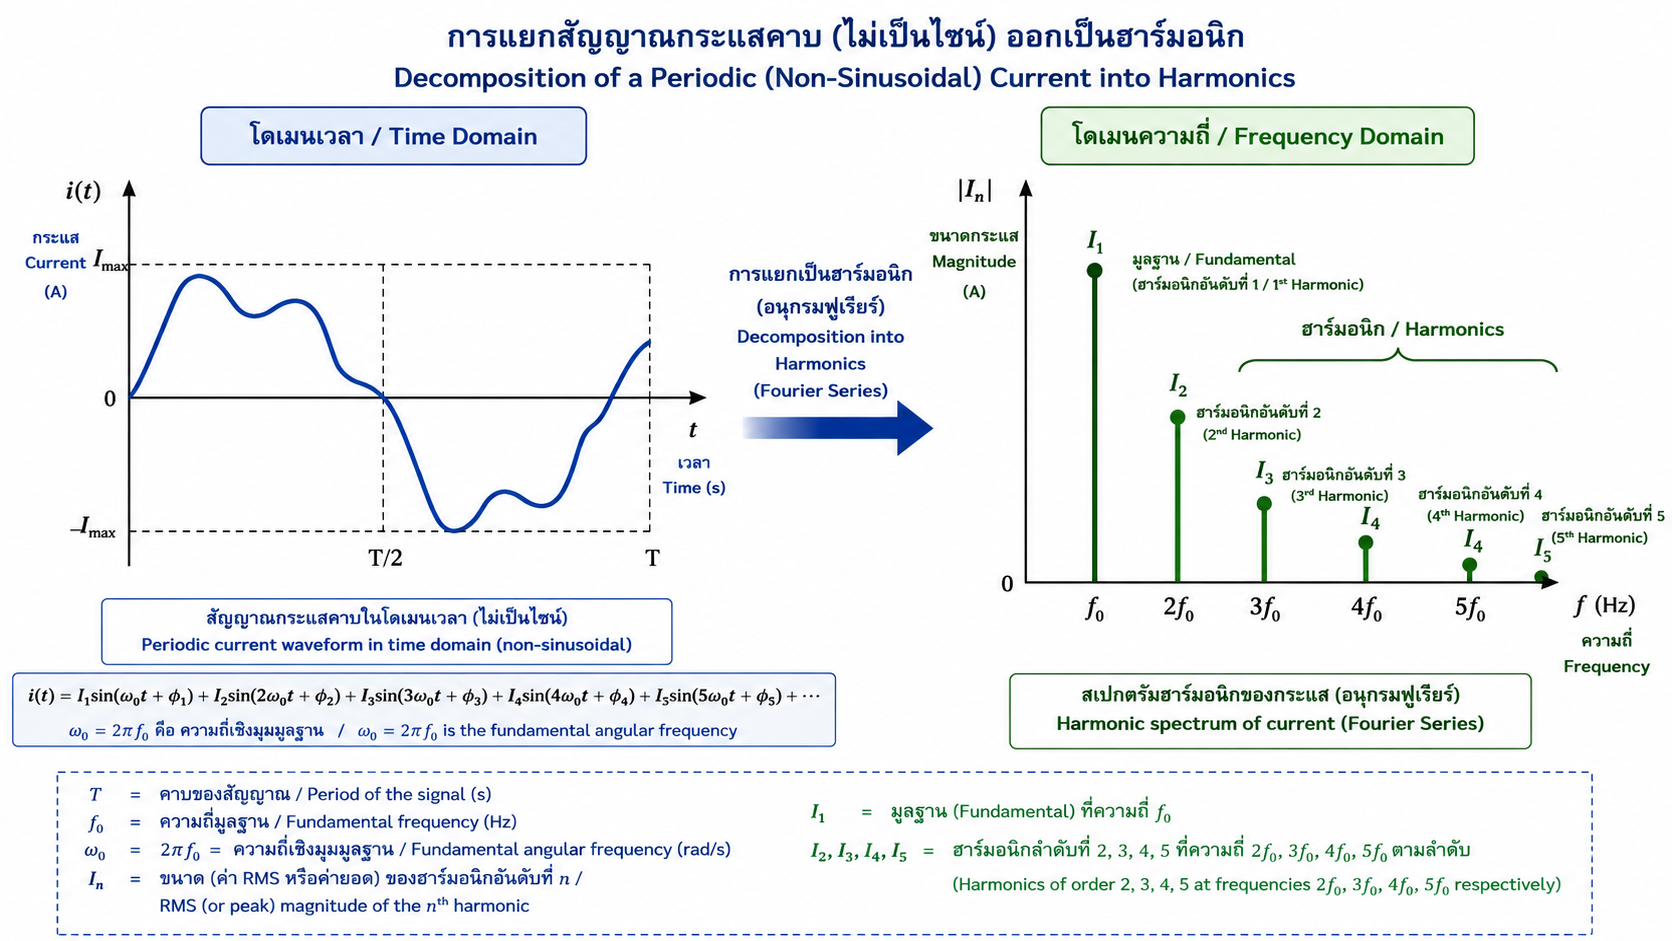
\includegraphics[width=0.8\textwidth]{images/chapter5/figure-01.png}
    \caption{กราฟผลตอบสนองต่อสัญญาณขั้นบันไดของระบบอันดับหนึ่ง}
\end{figure}



\textbf{ตัวอย่างที่ 1 (พื้นฐาน): การหาค่าคงเวลาและเวลาที่ผลตอบสนองเข้าใกล้ค่าสุดท้าย}

โจทย์: ระบบวงปิดมีฟังก์ชันถ่ายโอน $T(s) = \dfrac{4}{s+4}$ จงหาค่าคงเวลา τ และเวลาที่ผลตอบสนองต่อสัญญาณขั้นบันไดหนึ่งหน่วยมีค่าถึง 90\% และ 95\% ของค่าสุดท้าย รวมถึง Settling Time ที่เกณฑ์ 2\%

\textit{ขั้นตอนที่ 1 วิเคราะห์ระบบ:} ระบบเป็นอันดับหนึ่ง มีโพลเดียวที่ $s=-4$

\textit{ขั้นตอนที่ 2 กำหนดตัวแปร:} ให้ $c(t)$ เป็นผลตอบสนองต่อสัญญาณขั้นบันไดหนึ่งหน่วย

\textit{ขั้นตอนที่ 3 เลือกหลักการ:} จัดรูป $T(s)$ ให้อยู่ในรูปมาตรฐาน $K/(\tau s+1)$

\textit{ขั้นตอนที่ 4 สร้างสมการ:} หารเศษและส่วนด้วย 4

\[
T(s) = \frac{4}{s+4} = \frac{1}{0.25s+1}
\]

\textit{ขั้นตอนที่ 5 จัดรูปสมการ:} เทียบกับรูปมาตรฐานได้ $\tau = 0.25$ วินาที และ $K=1$

\textit{ขั้นตอนที่ 6 แทนค่า/แปลงโดเมน:} ใช้ $c(t) = 1-e^{-t/\tau}$ ตั้งสมการหาค่า $t$ ที่ $c(t)=0.90$ และ $c(t)=0.95$

\[
1-e^{-t/\tau} = 0.90 \;\Rightarrow\; e^{-t/\tau} = 0.10 \;\Rightarrow\; t = \tau \ln(10)
\]

\[
1-e^{-t/\tau} = 0.95 \;\Rightarrow\; e^{-t/\tau} = 0.05 \;\Rightarrow\; t = \tau \ln(20)
\]

\textit{ขั้นตอนที่ 7 คำนวณ:}

\[
t_{90\%} = 0.25 \times 2.3026 = 0.576 \text{ s}, \qquad t_{95\%} = 0.25 \times 2.9957 = 0.749 \text{ s}
\]

Settling Time ที่เกณฑ์ 2\% ประมาณจาก $t_s \approx 4\tau = 4 \times 0.25 = 1.0$ วินาที

\textit{ขั้นตอนที่ 8 ตรวจสอบหน่วยและความสมเหตุสมผล:} หน่วยเป็นวินาทีสอดคล้องกับนิยามของเวลา และค่า $t_{90\%} < t_{95\%} < t_s$ ซึ่งเป็นไปตามลำดับที่ควรจะเป็น

\textit{ขั้นตอนที่ 9 แปลความหมาย:} ระบบนี้มีค่าคงเวลาเพียง 0.25 วินาที จึงเป็นระบบที่ตอบสนองเร็ว โดยจะเข้าใกล้ค่าสุดท้ายเกือบสมบูรณ์ภายในเวลาประมาณ 1 วินาที



\subsubsection{7.2 ผลตอบสนองของระบบอันดับสอง (Second-Order System Response)}

ระบบทางวิศวกรรมจำนวนมาก เช่น ระบบมอเตอร์ไฟฟ้าที่มีความเฉื่อยและความหน่วง หรือวงจร RLC มีฟังก์ชันถ่ายโอนแบบอันดับสอง ซึ่งเขียนในรูปมาตรฐาน (Standard Second-Order Form) ได้เป็น

\[
G(s) = \frac{\omega_n^2}{s^2 + 2\zeta\omega_n s + \omega_n^2}
\]

โดยที่

\begin{itemize}
    \item $\omega_n$ คือ \textbf{ความถี่ธรรมชาติไม่หน่วง (Undamped Natural Frequency)} มีหน่วยเป็น rad/s คือความถี่ที่ระบบจะแกว่งหากไม่มีความหน่วงใด ๆ
    \item $\zeta$ (ซีตา) คือ \textbf{อัตราส่วนหน่วง (Damping Ratio)} เป็นค่าไม่มีหน่วย บ่งชี้ระดับการหน่วงของระบบเทียบกับการหน่วงวิกฤต
\end{itemize}

สมการเอกลักษณ์ (Characteristic Equation) ของระบบคือ

\[
s^2 + 2\zeta\omega_n s + \omega_n^2 = 0
\]

แก้สมการหาโพลได้

\[
s_{1,2} = -\zeta\omega_n \pm \omega_n\sqrt{\zeta^2-1}
\]

\textbf{สมมติฐานและเงื่อนไขการใช้งาน:} สูตรและข้อกำหนดสมรรถนะในบทนี้อ้างอิงจากระบบอันดับสองมาตรฐานที่ไม่มีซีโรจำกัด (Finite Zero) และไม่มีโพลเพิ่มเติมอื่นนอกเหนือจากคู่โพลหลัก หากระบบจริงมีซีโรหรือโพลเพิ่มเติมที่อยู่ใกล้คู่โพลหลัก ค่าที่คำนวณได้จากสูตรเหล่านี้จะเป็นเพียงค่าประมาณ


\subsubsection{7.3 ประเภทของการตอบสนอง (Response Types)}

ค่าอัตราส่วนหน่วง $\zeta$ เป็นตัวกำหนดตำแหน่งของโพลบนระนาบ s และรูปแบบของผลตอบสนอง แบ่งออกเป็น 4 กรณี

\textbf{กรณีที่ 1: ไม่มีการหน่วง (Undamped, $\zeta = 0$)}
โพลเป็นจำนวนจินตภาพล้วน $s_{1,2}=\pm j\omega_n$ ระบบแกว่งตลอดไปโดยไม่ลดขนาดลง ไม่พบในระบบจริงที่มีการสูญเสียพลังงาน แต่ใช้เป็นกรณีอ้างอิงทางทฤษฎี

\textbf{กรณีที่ 2: หน่วงน้อยกว่าวิกฤต (Underdamped, $0 < \zeta < 1$)}
โพลเป็นจำนวนเชิงซ้อนคู่สังยุค

\[
s_{1,2} = -\zeta\omega_n \pm j\omega_n\sqrt{1-\zeta^2} = -\zeta\omega_n \pm j\omega_d
\]

โดยนิยาม \textbf{ความถี่หน่วง (Damped Frequency)}

\[
\omega_d = \omega_n\sqrt{1-\zeta^2}
\]

ผลตอบสนองต่อสัญญาณขั้นบันไดหนึ่งหน่วยมีรูปแบบ

\[
c(t) = 1 - \frac{e^{-\zeta\omega_n t}}{\sqrt{1-\zeta^2}}\sin(\omega_d t + \theta), \qquad \theta = \cos^{-1}\zeta
\]

ผลตอบสนองแบบนี้มีลักษณะแกว่งพุ่งเกินค่าสุดท้ายก่อนสงบนิ่งเข้าสู่ค่าคงตัว เป็นกรณีที่พบบ่อยที่สุดในระบบควบคุมจริงและเป็นกรณีหลักที่ใช้นิยามข้อกำหนดสมรรถนะในหัวข้อ 7.4

\textbf{กรณีที่ 3: หน่วงวิกฤต (Critically Damped, $\zeta = 1$)}
โพลซ้ำเป็นจำนวนจริง $s_{1,2}=-\omega_n$ ผลตอบสนองไม่มีการแกว่งและเข้าสู่ค่าคงตัวได้เร็วที่สุดในบรรดาระบบที่ไม่มีการพุ่งเกิน

\textbf{กรณีที่ 4: หน่วงมากกว่าวิกฤต (Overdamped, $\zeta > 1$)}
โพลเป็นจำนวนจริงสองค่าที่แตกต่างกัน

\[
s_{1,2} = -\zeta\omega_n \pm \omega_n\sqrt{\zeta^2-1}
\]

ผลตอบสนองเป็นผลรวมของเลขชี้กำลังสองพจน์ ไม่มีการแกว่ง แต่เข้าสู่ค่าคงตัวช้ากว่ากรณีหน่วงวิกฤต

% [รูปที่ 2: ตำแหน่งโพลบนระนาบ s สำหรับกรณีการหน่วงต่าง ๆ]
% ประเภทภาพ: Technical Illustration
% ตำแหน่งที่แนะนำ: หลังการอธิบายทั้งสี่กรณีในหัวข้อ 7.3
% วัตถุประสงค์การเรียนรู้: ให้ผู้เรียนเชื่อมโยงค่า ζ กับตำแหน่งโพลบนระนาบ s ได้โดยตรง
% คำอธิบายภาพ: ระนาบ s แสดงแกนจริง (Re) แนวนอนและแกนจินตภาพ (Im) แนวตั้ง แสดงตำแหน่งโพล 4 ชุด ได้แก่ โพลบนแกนจินตภาพ (ζ=0), โพลเชิงซ้อนคู่สังยุคในครึ่งซ้าย (0<ζ<1) พร้อมมุม θ จากแกนจินตภาพลบ, โพลซ้ำบนแกนจริงลบ (ζ=1), และโพลจริงสองตำแหน่งบนแกนจริงลบที่ระยะห่างต่างกัน (ζ>1)
% องค์ประกอบที่ต้องมี: แกน Re, แกน Im, จุดกากบาทแทนตำแหน่งโพลแต่ละกรณี, เส้นประรัศมี ωn จากจุดกำเนิดถึงโพลเชิงซ้อน, มุม θ = cos⁻¹ζ
% ข้อความหรือป้ายกำกับ: "ζ=0", "0<ζ<1", "ζ=1", "ζ>1", "ωn", "θ", "Re", "Im"
% ภาษาของป้ายกำกับ: ไทยและอังกฤษ
% สัดส่วนภาพ: 4:3
% Image Generation Prompt: Technical diagram of the complex s-plane showing pole locations for four damping cases: purely imaginary poles, complex conjugate pole pair in the left half plane with angle theta from the negative imaginary axis, repeated real pole, and two distinct real poles further left, engineering textbook style, labeled axes, minimalist line art
% Alt Text: แผนภาพระนาบ s แสดงตำแหน่งโพลสำหรับกรณี Undamped, Underdamped, Critically Damped และ Overdamped

\begin{figure}[htbp]
    \centering
    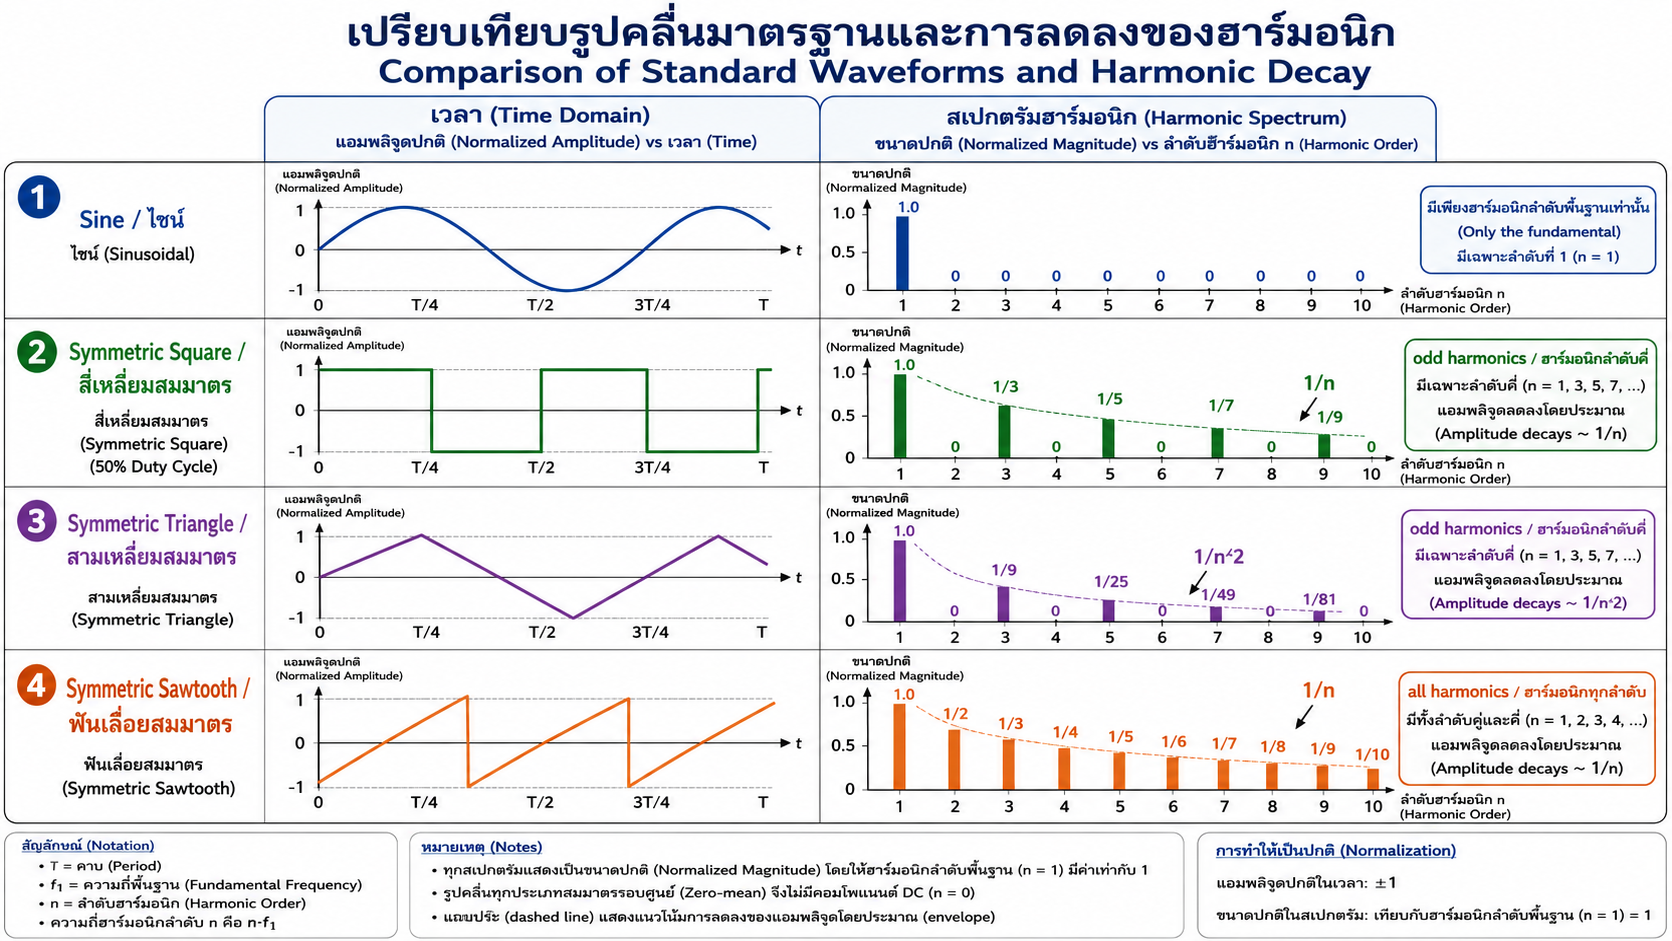
\includegraphics[width=0.8\textwidth]{images/chapter5/figure-02.png}
    \caption{ตำแหน่งโพลบนระนาบ s สำหรับกรณีการหน่วงต่าง ๆ}
\end{figure}

% [รูปที่ 3: กราฟเปรียบเทียบผลตอบสนองต่อสัญญาณขั้นบันไดสำหรับค่า ζ ต่าง ๆ]
% ประเภทภาพ: Graph
% ตำแหน่งที่แนะนำ: ต่อจากรูปที่ 2 ในหัวข้อ 7.3
% วัตถุประสงค์การเรียนรู้: ให้ผู้เรียนเห็นภาพรวมว่าเมื่อ ζ เปลี่ยนแปลง รูปร่างของกราฟผลตอบสนองเปลี่ยนไปอย่างไร
% คำอธิบายภาพ: กราฟแกนนอนเป็นเวลา $\omega_n t$ (Normalized Time) แกนตั้งเป็น c(t) มีเส้นกราฟหลายเส้นซ้อนกันสำหรับ ζ = 0 (แกว่งไม่ลดทอน), ζ = 0.2, ζ = 0.5, ζ = 0.7 (Underdamped ระดับต่าง ๆ), ζ = 1 (Critically Damped), ζ = 2 (Overdamped)
% องค์ประกอบที่ต้องมี: แกน ωn t, แกน c(t), เส้นกำกับ c(t)=1, เส้นกราฟหลายสีพร้อม Legend ระบุค่า ζ ของแต่ละเส้น
% ข้อความหรือป้ายกำกับ: "ζ=0", "ζ=0.2", "ζ=0.5", "ζ=0.7", "ζ=1", "ζ=2", "ωn t", "c(t)"
% ภาษาของป้ายกำกับ: ไทยและอังกฤษ
% สัดส่วนภาพ: 16:9
% Image Generation Prompt: Family of step response curves for a standard second order system at damping ratios 0, 0.2, 0.5, 0.7, 1, and 2, overlaid on one graph with normalized time axis, color-coded legend, engineering textbook style, clean white background
% Graph Generation Prompt: พล็อตสมการ $c(t)=1-\dfrac{e^{-\zeta\omega_n t}}{\sqrt{1-\zeta^2}}\sin(\omega_d t+\theta)$ สำหรับ ζ=0.2,0.5,0.7 และสมการกรณี ζ=1, ζ=2 ตามลำดับ ช่วงเวลา $\omega_n t \in [0,15]$ แกนตั้ง c(t) ตั้งแต่ 0 ถึงประมาณ 1.6
% Alt Text: กราฟเปรียบเทียบผลตอบสนองต่อสัญญาณขั้นบันไดของระบบอันดับสองที่ค่าอัตราส่วนหน่วงต่างกันหกค่า

\begin{figure}[htbp]
    \centering
    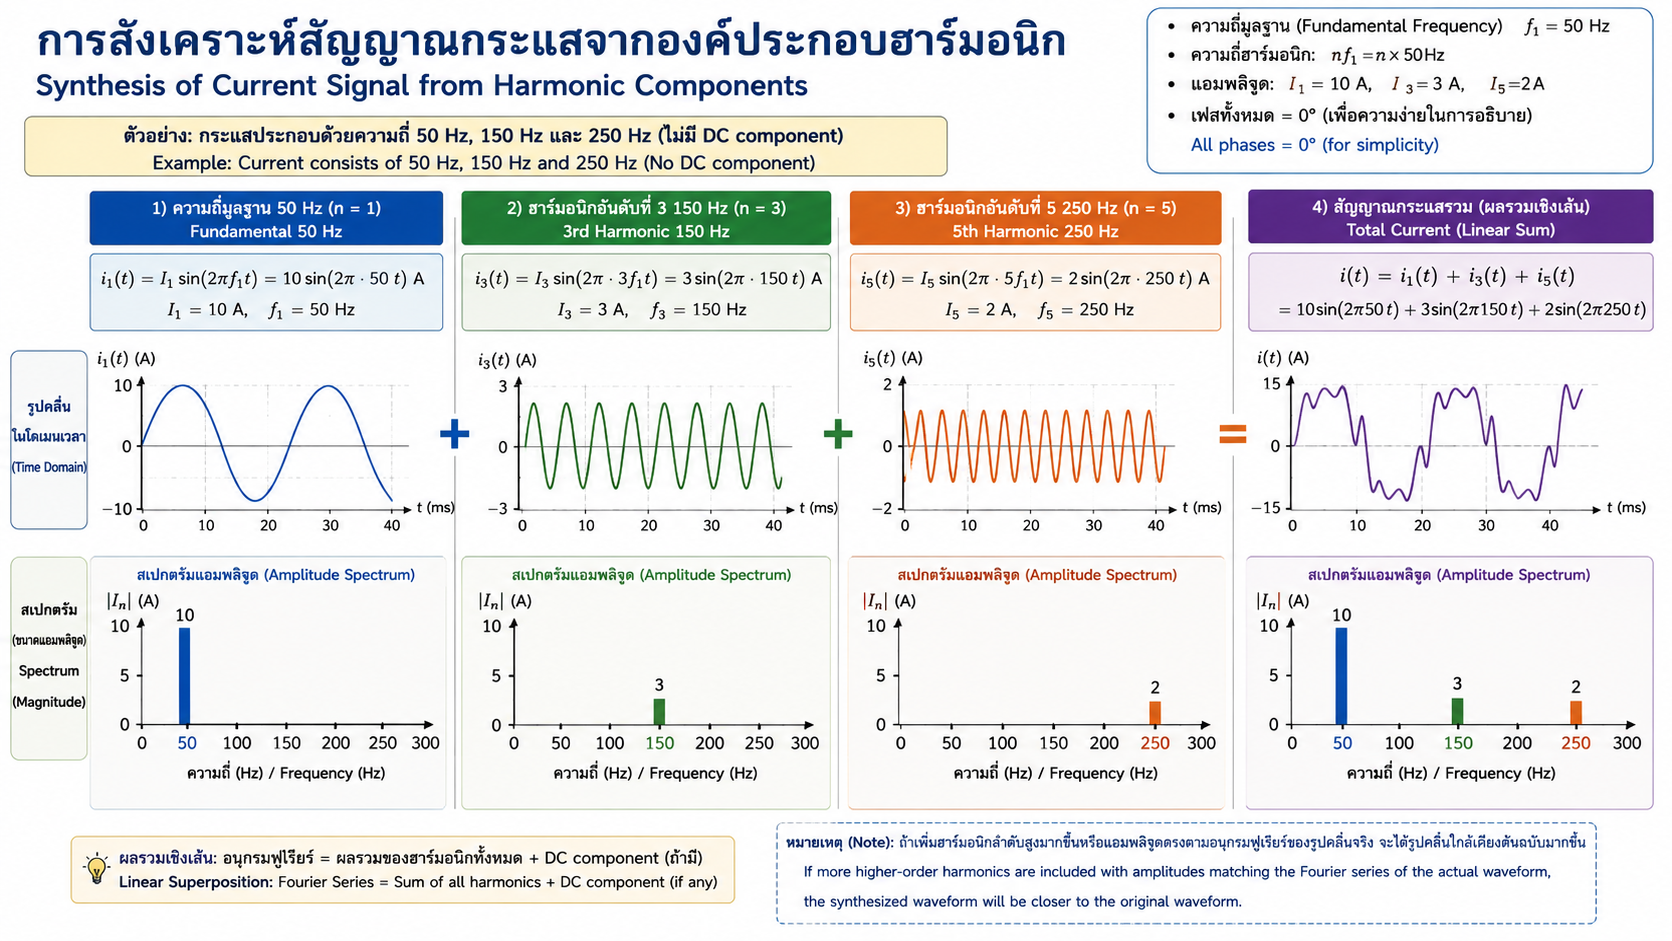
\includegraphics[width=0.8\textwidth]{images/chapter5/figure-03.png}
    \caption{กราฟเปรียบเทียบผลตอบสนองต่อสัญญาณขั้นบันไดสำหรับค่า ζ ต่าง ๆ}
\end{figure}



\textbf{ตัวอย่างที่ 2 (เชิงวิเคราะห์): การจำแนกประเภทการตอบสนองจากฟังก์ชันถ่ายโอน}

โจทย์: ระบบวงปิดมีฟังก์ชันถ่ายโอน $T(s) = \dfrac{36}{s^2+4.2s+36}$ จงหาค่า ζ, ωn, ωd และตำแหน่งโพล พร้อมระบุประเภทของการตอบสนอง

\textit{ขั้นตอนที่ 1 วิเคราะห์ระบบ:} เป็นระบบอันดับสองในรูปมาตรฐานอยู่แล้ว

\textit{ขั้นตอนที่ 2 กำหนดตัวแปร:} เทียบสัมประสิทธิ์กับ $\omega_n^2/(s^2+2\zeta\omega_n s+\omega_n^2)$

\textit{ขั้นตอนที่ 3 เลือกหลักการ:} การเทียบสัมประสิทธิ์พหุนามตัวส่วน

\textit{ขั้นตอนที่ 4 สร้างสมการ:} $\omega_n^2 = 36$ และ $2\zeta\omega_n = 4.2$

\textit{ขั้นตอนที่ 5 จัดรูปสมการ:} $\omega_n = \sqrt{36} = 6$ rad/s และ $\zeta = 4.2/(2\times 6)$

\textit{ขั้นตอนที่ 6 แทนค่า:} $\zeta = 4.2/12 = 0.35$

\textit{ขั้นตอนที่ 7 คำนวณ:}

\[
\omega_d = \omega_n\sqrt{1-\zeta^2} = 6\sqrt{1-0.1225} = 6\times 0.9367 = 5.62 \text{ rad/s}
\]

\[
s_{1,2} = -\zeta\omega_n \pm j\omega_d = -2.1 \pm j5.62
\]

\textit{ขั้นตอนที่ 8 ตรวจสอบความสมเหตุสมผล:} $0 < \zeta = 0.35 < 1$ และโพลเป็นจำนวนเชิงซ้อนคู่สังยุคในครึ่งซ้ายของระนาบ s สอดคล้องกับเกณฑ์ของกรณี Underdamped

\textit{ขั้นตอนที่ 9 แปลความหมาย:} ระบบนี้เป็น \textbf{Underdamped} จะมีผลตอบสนองแกว่งพุ่งเกินค่าสุดท้ายก่อนสงบนิ่งเข้าสู่ค่าคงตัว โดยความถี่ที่สังเกตเห็นการแกว่งจริงคือ ωd = 5.62 rad/s ไม่ใช่ ωn = 6 rad/s


\subsubsection{7.4 ข้อกำหนดสมรรถนะ (Performance Specifications)}

สำหรับระบบอันดับสองแบบ Underdamped ซึ่งเป็นกรณีที่ใช้ในการออกแบบจริงมากที่สุด วิศวกรกำหนดคุณภาพของผลตอบสนองด้วยตัวชี้วัด 4 ค่า ดังนี้

\textbf{เวลาสูงสุด (Peak Time, $t_p$)}

คือเวลาที่ผลตอบสนองมีค่าสูงสุดครั้งแรก หาได้จากการหาอนุพันธ์ของ $c(t)$ เทียบกับเวลาแล้วให้เท่ากับศูนย์

\[
t_p = \frac{\pi}{\omega_d} = \frac{\pi}{\omega_n\sqrt{1-\zeta^2}}
\]

\textbf{เปอร์เซ็นต์การพุ่งเกิน (Percent Overshoot, \%OS)}

คือร้อยละของค่าที่ผลตอบสนองพุ่งเกินค่าสุดท้ายเทียบกับค่าสุดท้าย

\[
\%OS = e^{-\zeta\pi/\sqrt{1-\zeta^2}} \times 100
\]

ข้อสังเกตสำคัญคือ \textbf{\%OS ขึ้นอยู่กับ ζ เพียงตัวแปรเดียว} ไม่ขึ้นกับ ωn หรือขนาดของสัญญาณเข้า ทำให้สามารถแก้สมการย้อนกลับเพื่อหา ζ ที่ต้องการจากค่า \%OS ที่กำหนดในข้อกำหนดการออกแบบได้

\[
\zeta = \frac{-\ln(\%OS/100)}{\sqrt{\pi^2 + \ln^2(\%OS/100)}}
\]

\textbf{เวลาเข้าสู่ภาวะคงตัว (Settling Time, $t_s$)}

คือเวลาที่ผลตอบสนองเข้าไปอยู่ในช่วง ±2\% (หรือ ±5\% ตามเกณฑ์ที่เลือกใช้) รอบค่าสุดท้ายอย่างถาวร ประมาณจากเปลือกเลขชี้กำลัง (Envelope) ของผลตอบสนอง $e^{-\zeta\omega_n t}$

\[
t_s \approx \frac{4}{\zeta\omega_n} \quad \text{(เกณฑ์ 2\%)} \qquad \text{หรือ} \qquad t_s \approx \frac{3}{\zeta\omega_n} \quad \text{(เกณฑ์ 5\%)}
\]

\textbf{ต้องระบุเกณฑ์ที่ใช้เสมอ} เนื่องจากค่า Settling Time ที่ได้จากทั้งสองเกณฑ์แตกต่างกัน

\textbf{เวลาขึ้น (Rise Time, $t_r$)}

สำหรับระบบ Underdamped นิยมนิยามเป็นเวลาที่ผลตอบสนองเพิ่มจาก 0\% ถึง 100\% ของค่าสุดท้ายเป็นครั้งแรก ค่าที่แม่นยำต้องแก้สมการ $c(t)=1$ ซึ่งไม่มีคำตอบรูปปิดอย่างง่าย โดยทั่วไปใช้ค่าประมาณ (Rule of Thumb) ที่ใช้ได้ดีในช่วง $0.3 \le \zeta \le 0.8$

\[
t_r \approx \frac{1.8}{\omega_n}
\]

หากต้องการค่าที่แม่นยำกว่านี้ หรือ ζ อยู่นอกช่วงดังกล่าว ควรหาคำตอบด้วยวิธีเชิงตัวเลขหรือใช้ MATLAB ตามหัวข้อ 7.6

% [รูปที่ 4: กราฟผลตอบสนองอันดับสองแบบ Underdamped พร้อมระบุข้อกำหนดสมรรถนะ]
% ประเภทภาพ: Graph
% ตำแหน่งที่แนะนำ: หลังการอธิบายครบทั้ง 4 ข้อกำหนดในหัวข้อ 7.4
% วัตถุประสงค์การเรียนรู้: ให้ผู้เรียนอ่านค่า tr, tp, %OS, ts จากกราฟได้โดยตรงก่อนเชื่อมโยงเข้าสู่สูตรคำนวณ
% คำอธิบายภาพ: กราฟผลตอบสนองต่อสัญญาณขั้นบันไดแบบ Underdamped เส้นโค้งเริ่มจาก 0 พุ่งขึ้นแกว่งเกินเส้นค่าสุดท้าย (c=1) แล้วแกว่งลดขนาดลงจนสงบนิ่ง มีเส้นประระบุตำแหน่ง tr (จุดแรกที่ถึง c=1), tp และ Peak Value สูงสุด, แถบสีบาง ๆ รอบ c=1 กว้าง ±2% แสดงขอบเขต Settling Time พร้อมเส้นประแนวตั้งที่ตำแหน่ง ts ซึ่งกราฟเข้าไปอยู่ในแถบอย่างถาวร
% องค์ประกอบที่ต้องมี: แกน t, แกน c(t), เส้นค่าสุดท้าย c=1, แถบ ±2% รอบ c=1, จุดยอด (Peak), เส้นประระบุ tr, tp, ts
% ข้อความหรือป้ายกำกับ: "tr", "tp", "ts", "%OS", "c(t)=1", "±2%"
% ภาษาของป้ายกำกับ: ไทยและอังกฤษ
% สัดส่วนภาพ: 16:9
% Image Generation Prompt: Annotated underdamped second order step response curve showing rise time, peak time with peak value overshoot, percent overshoot bracket, a shaded plus-minus two percent settling band around the final value, and settling time marker, engineering textbook diagram style, clean labeled axes
% Graph Generation Prompt: พล็อต $c(t)=1-\dfrac{e^{-\zeta\omega_n t}}{\sqrt{1-\zeta^2}}\sin(\omega_d t+\theta)$ โดยใช้ ζ=0.35, ωn=6 (จากตัวอย่างที่ 2) ช่วงเวลา $t\in[0,2.5]$ วินาที ทำเครื่องหมายที่ tr, tp, ts และแถบ ±2%
% Alt Text: กราฟผลตอบสนองอันดับสองแบบ Underdamped พร้อมป้ายกำกับเวลาขึ้น เวลาสูงสุด เปอร์เซ็นต์การพุ่งเกิน และเวลาเข้าสู่ภาวะคงตัว

\begin{figure}[htbp]
    \centering
    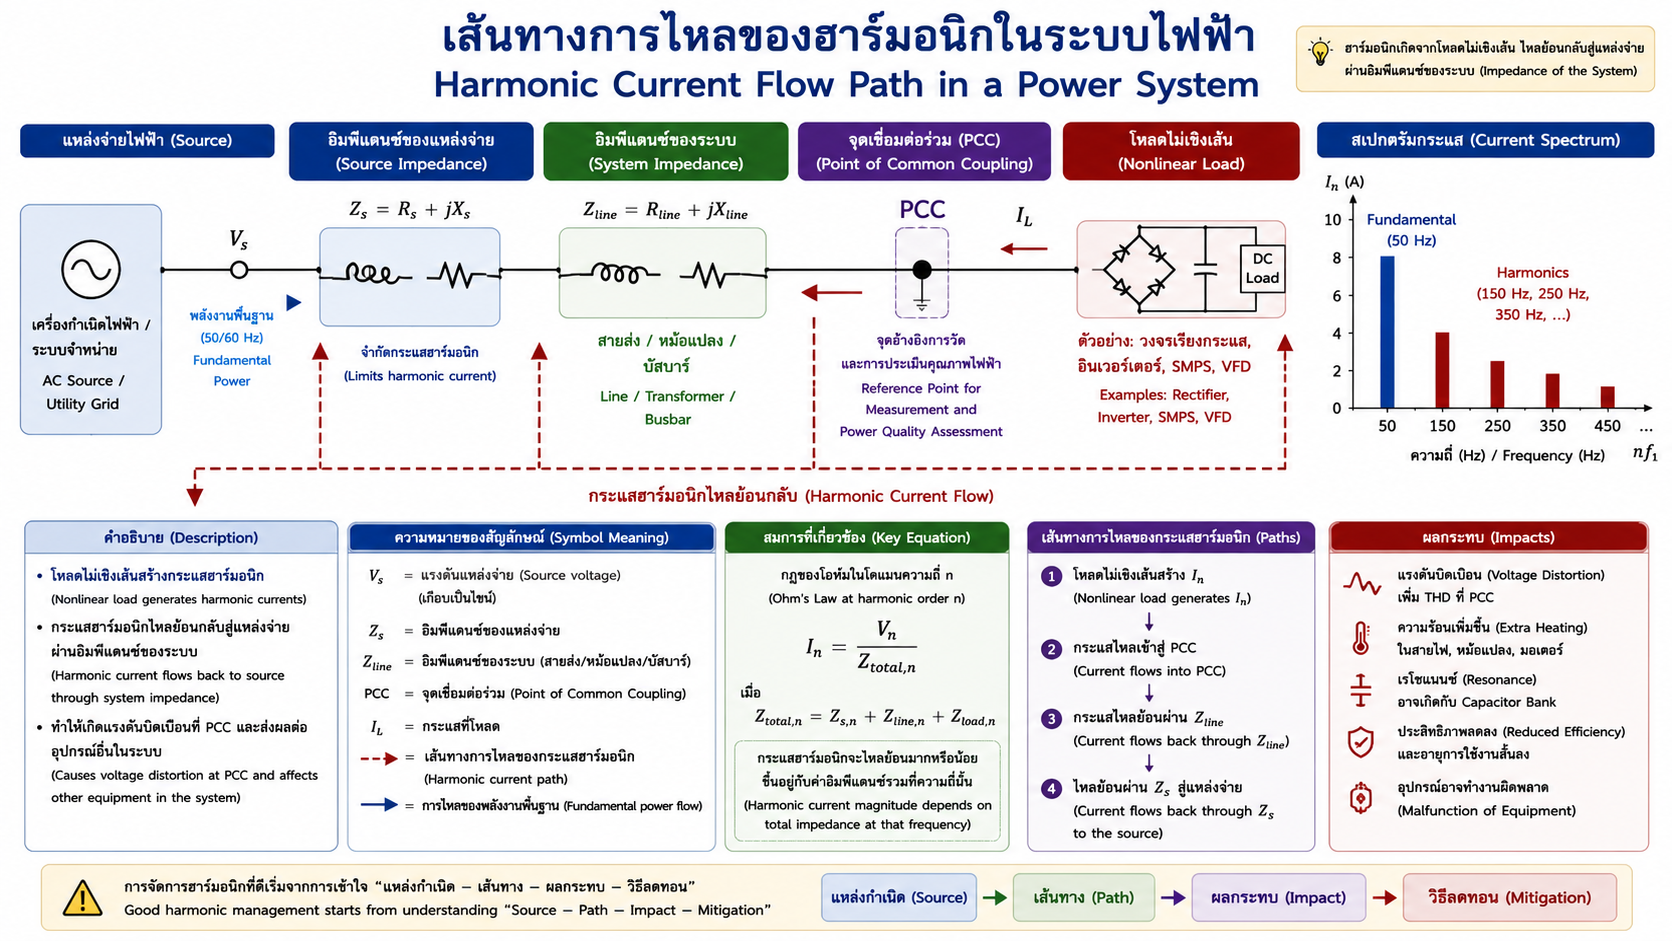
\includegraphics[width=0.8\textwidth]{images/chapter5/figure-04.png}
    \caption{กราฟผลตอบสนองอันดับสองแบบ Underdamped พร้อมระบุข้อกำหนดสมรรถนะ}
\end{figure}



\textbf{ตัวอย่างที่ 3 (เชิงวิเคราะห์): การคำนวณข้อกำหนดสมรรถนะ}

โจทย์: จากระบบในตัวอย่างที่ 2 ($\zeta=0.35$, $\omega_n=6$ rad/s, $\omega_d=5.62$ rad/s) จงคำนวณ $t_p$, $\%OS$, $t_s$ (เกณฑ์ 2\%) และ $t_r$ โดยประมาณ

\textit{ขั้นตอนที่ 1 วิเคราะห์ระบบ:} ใช้พารามิเตอร์ ζ, ωn, ωd ที่ได้จากตัวอย่างที่ 2

\textit{ขั้นตอนที่ 2 กำหนดตัวแปร:} ใช้สูตรข้อกำหนดสมรรถนะทั้งสี่

\textit{ขั้นตอนที่ 3 เลือกหลักการ:} สูตร $t_p=\pi/\omega_d$, $\%OS=e^{-\zeta\pi/\sqrt{1-\zeta^2}}\times100$, $t_s=4/(\zeta\omega_n)$, $t_r\approx1.8/\omega_n$

\textit{ขั้นตอนที่ 4–5 สร้างและจัดรูปสมการ:} แทนค่าพารามิเตอร์ลงในแต่ละสูตรโดยตรง

\textit{ขั้นตอนที่ 6–7 แทนค่าและคำนวณ:}

\[
t_p = \frac{\pi}{5.62} = 0.559 \text{ s}
\]

\[
\%OS = e^{-0.35\pi/\sqrt{1-0.1225}} \times 100 = e^{-1.174}\times100 = 30.9\%
\]

\[
t_s = \frac{4}{0.35\times6} = \frac{4}{2.1} = 1.90 \text{ s}
\]

\[
t_r \approx \frac{1.8}{6} = 0.30 \text{ s}
\]

\textit{ขั้นตอนที่ 8 ตรวจสอบความสมเหตุสมผล:} ค่า $t_r < t_p < t_s$ เป็นลำดับที่สมเหตุสมผล เพราะระบบต้องขึ้นถึงค่าสุดท้ายก่อน จึงจะแกว่งถึงจุดสูงสุด แล้วจึงค่อยสงบนิ่ง และ ζ=0.35 อยู่ในช่วงที่สูตรประมาณ $t_r$ ใช้ได้ดี (0.3–0.8)

\textit{ขั้นตอนที่ 9 แปลความหมาย:} ระบบนี้จะพุ่งเกินค่าสุดท้ายถึง 30.9\% ซึ่งค่อนข้างสูง และใช้เวลาเกือบ 2 วินาทีกว่าจะสงบนิ่งเข้าสู่ค่าคงตัว หากข้อกำหนดของงานต้องการ \%OS ที่ต่ำกว่านี้ จำเป็นต้องปรับค่า ζ ให้สูงขึ้น ดังแสดงในตัวอย่างถัดไป



\textbf{ตัวอย่างที่ 4 (ประยุกต์ใช้): การออกแบบค่าอัตราขยาย K ให้เป็นไปตามข้อกำหนดสมรรถนะ}

โจทย์: ระบบควบคุมความเร็วมอเตอร์มีฟังก์ชันถ่ายโอนวงเปิด $G(s)=\dfrac{K}{s(s+6)}$ ต่อแบบป้อนกลับหนึ่งหน่วย (Unity Feedback) ข้อกำหนดของงานต้องการ $\%OS \le 16\%$ และ $t_s \le 2$ วินาที (เกณฑ์ 2\%) โดยพิจารณาเฉพาะกรณีที่ระบบมีลักษณะ Underdamped จงหาช่วงค่า K ที่เป็นไปได้

\textit{ขั้นตอนที่ 1 วิเคราะห์ระบบ:} หาฟังก์ชันถ่ายโอนวงปิดก่อน

\[
T(s) = \frac{G(s)}{1+G(s)} = \frac{K}{s^2+6s+K}
\]

\textit{ขั้นตอนที่ 2 กำหนดตัวแปร:} เทียบกับรูปมาตรฐานได้ $\omega_n^2=K$ และ $2\zeta\omega_n=6 \Rightarrow \zeta\omega_n=3$ (ค่าคงที่ ไม่ขึ้นกับ K)

\textit{ขั้นตอนที่ 3 เลือกหลักการ:} ใช้สูตร \%OS หาค่า ζ ต่ำสุดที่ยอมรับได้ก่อน แล้วจึงหา ωn และ K

\textit{ขั้นตอนที่ 4–5 สร้างและจัดรูปสมการ:} จากสูตรผกผัน

\[
\zeta_{min} = \frac{-\ln(0.16)}{\sqrt{\pi^2+\ln^2(0.16)}}
\]

\textit{ขั้นตอนที่ 6 แทนค่า:} $\ln(0.16) = -1.833$

\[
\zeta_{min} = \frac{1.833}{\sqrt{9.870+3.358}} = \frac{1.833}{\sqrt{13.228}} = \frac{1.833}{3.637} = 0.504
\]

\textit{ขั้นตอนที่ 7 คำนวณ:} เนื่องจาก $\zeta\omega_n=3$ คงที่ ดังนั้น $\omega_n = 3/\zeta$ เมื่อ $\zeta \ge 0.504$ จะได้

\[
\omega_n \le \frac{3}{0.504} = 5.95 \text{ rad/s} \;\Rightarrow\; K=\omega_n^2 \le 35.4
\]

ตรวจสอบเงื่อนไข Underdamped ($\zeta<1$): ที่ $\zeta=1$ จะได้ $\omega_n=3$ rad/s หรือ $K=9$ ดังนั้นต้องมี $K>9$

ตรวจสอบ Settling Time: เนื่องจาก $\zeta\omega_n=3$ คงที่เสมอในระบบนี้ (ไม่ขึ้นกับ K) จะได้ $t_s=4/(\zeta\omega_n)=4/3=1.33$ วินาที ซึ่ง\textbf{น้อยกว่า 2 วินาทีเสมอ} ไม่ว่า K จะมีค่าใดในช่วง Underdamped

\textit{ขั้นตอนที่ 8 ตรวจสอบความสมเหตุสมผล:} ผลลัพธ์แสดงว่า Settling Time ของระบบนี้ถูกกำหนดตายตัวโดยตำแหน่งโพลที่ $s=-6$ ของระบบวงเปิด ซึ่งปรับด้วยค่า K เพียงอย่างเดียวไม่ได้ เป็นข้อจำกัดเชิงโครงสร้างของระบบที่ควรตระหนัก

\textit{ขั้นตอนที่ 9 แปลความหมาย:} ค่า K ที่ทำให้ระบบเป็นไปตามข้อกำหนดทั้งสองข้อ (โดยยังคง Underdamped) คือ \textbf{$9 < K \le 35.4$} โดย Settling Time จะเป็นไปตามข้อกำหนดโดยอัตโนมัติในช่วงนี้ หากต้องการปรับ Settling Time ให้เร็วขึ้นอีก จำเป็นต้องเปลี่ยนโครงสร้างของตัวควบคุม ไม่ใช่ปรับเพียงค่า K


\subsubsection{7.5 ความผิดพลาดคงตัว (Steady-State Error)}

นอกจากพฤติกรรมชั่วครู่แล้ว วิศวกรยังต้องพิจารณาว่าเมื่อเวลาผ่านไปนานพอ ผลตอบสนองของระบบจะติดตามสัญญาณอ้างอิงได้แม่นยำเพียงใด ผลต่างนี้เรียกว่า \textbf{ความผิดพลาดคงตัว (Steady-State Error, $e_{ss}$)}

\textbf{การหา ess ด้วยทฤษฎีบทค่าสุดท้าย}

สำหรับระบบป้อนกลับหนึ่งหน่วย (Unity Feedback) สัญญาณความผิดพลาดคือ

\[
E(s) = \frac{R(s)}{1+G(s)}
\]

ใช้ทฤษฎีบทค่าสุดท้าย (Final Value Theorem) จะได้

\[
e_{ss} = \lim_{t\to\infty} e(t) = \lim_{s\to0} sE(s) = \lim_{s\to0}\frac{sR(s)}{1+G(s)}
\]

\textbf{System Type}

นิยาม \textbf{ชนิดของระบบ (System Type)} คือจำนวนโพลของฟังก์ชันถ่ายโอนวงเปิด $G(s)$ ที่ตำแหน่ง $s=0$ (จำนวนตัวรวมสัญญาณหรือ Integrator ในวงเปิด) เขียนแทนด้วย $n$ ในรูปทั่วไป

\[
G(s) = \frac{K\prod(s+z_i)}{s^n\prod(s+p_j)}
\]

\textbf{ข้อควรระวัง:} System Type แตกต่างจากอันดับของระบบ (System Order) โดยสิ้นเชิง อันดับของระบบคือจำนวนโพลทั้งหมดของฟังก์ชันถ่ายโอนวงปิด ในขณะที่ System Type นับเฉพาะโพลที่ $s=0$ ของวงเปิดเท่านั้น

\textbf{ค่าคงที่ความผิดพลาด (Static Error Constants)}

\begin{table}[htbp]
    \centering
    \begin{tabular}{llll}
        \hline
        \textbf{ชื่อ} & \textbf{นิยาม} & \textbf{สัญญาณอ้างอิง} & \textbf{$e_{ss}$} \\
        \hline
        Position Error Constant & $K_p = \lim\limits_{s\to0} G(s)$ & ขั้นบันได $R(s)=1/s$ & $e_{ss} = \dfrac{1}{1+K_p}$ \\
        Velocity Error Constant & $K_v = \lim\limits_{s\to0} sG(s)$ & ทางลาด $R(s)=1/s^2$ & $e_{ss} = \dfrac{1}{K_v}$ \\
        Acceleration Error Constant & $K_a = \lim\limits_{s\to0} s^2G(s)$ & พาราโบลา $R(s)=1/s^3$ & $e_{ss} = \dfrac{1}{K_a}$ \\
        \hline
    \end{tabular}
\end{table}

\textbf{ความสัมพันธ์ระหว่าง System Type กับ ess}

\begin{table}[htbp]
    \centering
    \begin{tabular}{lrrr}
        \hline
        \textbf{System Type} & \textbf{$e_{ss}$ ต่อสัญญาณขั้นบันได} & \textbf{$e_{ss}$ ต่อสัญญาณทางลาด} & \textbf{$e_{ss}$ ต่อสัญญาณพาราโบลา} \\
        \hline
        Type 0 & จำกัด $= \dfrac{1}{1+K_p}$ & $\infty$ & $\infty$ \\
        Type 1 & $0$ & จำกัด $= \dfrac{1}{K_v}$ & $\infty$ \\
        Type 2 & $0$ & $0$ & จำกัด $= \dfrac{1}{K_a}$ \\
        \hline
    \end{tabular}
\end{table}

ตารางนี้แสดงหลักการสำคัญว่า \textbf{ระบบต้องมีตัวรวมสัญญาณอย่างน้อยเท่ากับดีกรีของสัญญาณอ้างอิง บวกหนึ่ง จึงจะติดตามสัญญาณนั้นได้โดยไม่มีความผิดพลาดคงตัว} เช่น การติดตามสัญญาณทางลาดโดยไม่มีความผิดพลาดคงตัวเลยต้องใช้ระบบ Type 2 ขึ้นไป



\textbf{ตัวอย่างที่ 5 (ประยุกต์ใช้): การหาชนิดของระบบและความผิดพลาดคงตัว}

โจทย์: ระบบป้อนกลับหนึ่งหน่วยมีฟังก์ชันถ่ายโอนวงเปิด $G(s)=\dfrac{20}{s(s+5)}$ จงหาชนิดของระบบ ค่า $K_p$, $K_v$, $K_a$ และความผิดพลาดคงตัวเมื่อป้อนสัญญาณทางลาดหนึ่งหน่วย $r(t)=t$

\textit{ขั้นตอนที่ 1 วิเคราะห์ระบบ:} $G(s)$ มีตัวประกอบ $s$ หนึ่งตัวในตัวส่วน จึงมีโพลที่ $s=0$ จำนวน 1 ตัว

\textit{ขั้นตอนที่ 2 กำหนดตัวแปร:} System Type $= 1$

\textit{ขั้นตอนที่ 3 เลือกหลักการ:} ใช้นิยาม $K_p$, $K_v$, $K_a$ ตามตาราง

\textit{ขั้นตอนที่ 4–5 สร้างและจัดรูปสมการ:}

\[
K_p = \lim_{s\to0} \frac{20}{s(s+5)} \to \infty \quad (\text{เนื่องจากตัวส่วนมี } s)
\]

\[
K_v = \lim_{s\to0} s\cdot\frac{20}{s(s+5)} = \lim_{s\to0}\frac{20}{s+5}
\]

\[
K_a = \lim_{s\to0} s^2\cdot\frac{20}{s(s+5)} = \lim_{s\to0}\frac{20s}{s+5}
\]

\textit{ขั้นตอนที่ 6–7 แทนค่าและคำนวณ:}

\[
K_v = \frac{20}{5} = 4, \qquad K_a = \frac{20\times0}{5} = 0
\]

ดังนั้น $e_{ss}(\text{step}) = \dfrac{1}{1+K_p} = 0$, $\quad e_{ss}(\text{ramp}) = \dfrac{1}{K_v} = \dfrac{1}{4} = 0.25$, $\quad e_{ss}(\text{parabola}) = \dfrac{1}{K_a} \to \infty$

\textit{ขั้นตอนที่ 8 ตรวจสอบความสมเหตุสมผล:} ผลลัพธ์สอดคล้องกับตารางในหัวข้อนี้พอดี เพราะระบบเป็น Type 1: $e_{ss}(\text{step})=0$, $e_{ss}(\text{ramp})$ มีค่าจำกัด, $e_{ss}(\text{parabola})=\infty$

\textit{ขั้นตอนที่ 9 แปลความหมาย:} เมื่อสั่งให้ระบบติดตามสัญญาณทางลาดหนึ่งหน่วย (เช่น ความเร็วอ้างอิงคงที่) ผลตอบสนองที่สภาวะคงตัวจะตามหลังสัญญาณอ้างอิงอยู่คงที่ 0.25 หน่วยเสมอ ซึ่งเป็นความผิดพลาดเชิงตำแหน่งที่ยอมรับได้หรือไม่ขึ้นอยู่กับข้อกำหนดของงานนั้น ๆ หากต้องการลดค่านี้ วิศวกรสามารถเพิ่มอัตราขยายวงเปิด (เพิ่มค่าคงที่ 20 ให้สูงขึ้น) เพื่อเพิ่ม $K_v$



\subsubsection{7.6 การจำลองผลตอบสนองด้วย MATLAB}

ซอฟต์แวร์ MATLAB พร้อม Control System Toolbox ช่วยให้วิเคราะห์ผลตอบสนองชั่วครู่และคำนวณข้อกำหนดสมรรถนะได้อย่างรวดเร็ว โดยไม่ต้องคำนวณด้วยมือทุกขั้นตอน ซึ่งมีประโยชน์อย่างยิ่งเมื่อต้องเปรียบเทียบหลายกรณีพร้อมกัน

\textbf{วัตถุประสงค์การใช้ซอฟต์แวร์:} สร้างฟังก์ชันถ่ายโอน พล็อตผลตอบสนองต่อสัญญาณขั้นบันได และคำนวณข้อกำหนดสมรรถนะโดยอัตโนมัติ เพื่อตรวจสอบผลการคำนวณด้วยมือและใช้เปรียบเทียบกับผลการทดลองจริงในกิจกรรมปฏิบัติการ

\begin{verbatim}
% กำหนดพารามิเตอร์ระบบอันดับสอง (ใช้ค่าจากตัวอย่างที่ 2-3)
zeta = 0.35;
wn = 6;

% สร้างฟังก์ชันถ่ายโอนในรูปมาตรฐาน
num = wn^2;
den = [1, 2*zeta*wn, wn^2];
sys = tf(num, den);

% พล็อตผลตอบสนองต่อสัญญาณขั้นบันได
figure;
step(sys);
grid on;
title('Step Response, \zeta = 0.35, \omega_n = 6 rad/s');

% คำนวณข้อกำหนดสมรรถนะโดยอัตโนมัติ
info = stepinfo(sys);
disp(info)
\end{verbatim}

คำสั่ง \texttt{stepinfo(sys)} จะคืนค่าโครงสร้างข้อมูลที่มีฟิลด์สำคัญ ได้แก่ \texttt{RiseTime}, \texttt{SettlingTime}, \texttt{Overshoot} (มีหน่วยเป็นเปอร์เซ็นต์อยู่แล้ว), \texttt{Peak} และ \texttt{PeakTime} ซึ่งควรมีค่าใกล้เคียงกับที่คำนวณด้วยมือในตัวอย่างที่ 3 (ความแตกต่างเล็กน้อยเกิดจาก MATLAB ใช้เกณฑ์ Settling Time เริ่มต้นที่ 2\% และคำนวณ Rise Time แบบ 0–100\% อย่างแม่นยำ ไม่ใช่ค่าประมาณ)

หากต้องการเปรียบเทียบผลตอบสนองสำหรับหลายค่า ζ พร้อมกันในกราฟเดียว (เช่นเดียวกับรูปที่ 3) สามารถวนลูปและใช้ \texttt{hold on} ได้ดังนี้

\begin{verbatim}
% เปรียบเทียบผลตอบสนองสำหรับหลายค่า zeta ที่ wn คงที่
wn = 6;
zeta_values = [0.2, 0.5, 0.7, 1.0, 2.0];

figure; hold on;
for z = zeta_values
    sys = tf(wn^2, [1, 2*z*wn, wn^2]);
    step(sys);
end
legend('\zeta=0.2', '\zeta=0.5', '\zeta=0.7', '\zeta=1.0', '\zeta=2.0');
grid on;
title('Step Response Comparison for Different Damping Ratios');
\end{verbatim}

\textbf{ค่าที่ผู้เรียนต้องปรับ:} \texttt{zeta}, \texttt{wn} ให้ตรงกับระบบที่กำลังวิเคราะห์ในแต่ละกรณี

\textbf{ผลลัพธ์ที่ควรสังเกต:} เมื่อ ζ เพิ่มขึ้น เส้นกราฟควรแกว่งน้อยลงและค่า Overshoot ที่ MATLAB คำนวณควรลดลงตามสูตรในหัวข้อ 7.4

\textbf{ข้อผิดพลาดที่พบบ่อย:} การลืมกำหนดลำดับสัมประสิทธิ์ในตัวแปร \texttt{den} ให้ถูกต้อง (ต้องเรียงจากดีกรีสูงไปต่ำ) และการสับสนระหว่างหน่วย Overshoot ที่ MATLAB แสดงเป็นเปอร์เซ็นต์อยู่แล้วกับสัดส่วน (Fraction) ที่บางครั้งใช้ในการคำนวณด้วยมือ

\textbf{ข้อจำกัด:} \texttt{stepinfo} ใช้เกณฑ์ Settling Time เริ่มต้นที่ 2\% และ Rise Time แบบ 0–100\% หากต้องการเปลี่ยนเกณฑ์ต้องระบุพารามิเตอร์เพิ่มเติม เช่น \texttt{stepinfo(sys,'SettlingTimeThreshold',0.05)} สำหรับเกณฑ์ 5\% ทั้งนี้คำสั่งและผลลัพธ์อาจแตกต่างกันเล็กน้อยระหว่างเวอร์ชันของ MATLAB จึงควรตรวจสอบกับเอกสารของเวอร์ชันที่ใช้งานจริง



\subsection{8. ความเข้าใจผิดที่พบบ่อย}

\textbf{ความเข้าใจผิดที่ 1:} ค่าคงเวลา τ คือเวลาที่ระบบเข้าสู่สภาวะคงตัวอย่างสมบูรณ์
\textbf{แนวคิดที่ถูกต้อง:} τ เป็นเพียงจุดอ้างอิงที่ระบบตอบสนองได้ 63.2\% ของค่าสุดท้ายเท่านั้น ระบบต้องใช้เวลาประมาณ 4τ ถึง 5τ จึงจะถือว่าเข้าสู่สภาวะคงตัวตามเกณฑ์ที่ยอมรับทั่วไป (2\% หรือ 1\%)

\textbf{ความเข้าใจผิดที่ 2:} Settling Time คำนวณด้วยเกณฑ์เดียวเสมอ
\textbf{แนวคิดที่ถูกต้อง:} ในทางปฏิบัติอาจใช้เกณฑ์ 2\% หรือ 5\% ขึ้นกับมาตรฐานหรือข้อตกลงของงานนั้น ๆ ผลลัพธ์ที่ได้จากสูตร $4/(\zeta\omega_n)$ และ $3/(\zeta\omega_n)$ จึงต่างกัน ต้องระบุเกณฑ์ที่ใช้กำกับไว้เสมอเพื่อไม่ให้สื่อสารคลาดเคลื่อน

\textbf{ความเข้าใจผิดที่ 3:} Percent Overshoot ขึ้นอยู่กับขนาดของสัญญาณเข้าหรือค่าสุดท้ายของผลตอบสนอง
\textbf{แนวคิดที่ถูกต้อง:} สำหรับระบบเชิงเส้นอันดับสองมาตรฐาน \%OS เป็นค่าสัดส่วน (Normalized) ที่ขึ้นอยู่กับ ζ เพียงตัวแปรเดียวเท่านั้น ไม่ว่าขนาดสัญญาณขั้นบันไดจะเป็นเท่าใด \%OS จะยังคงเท่าเดิมตราบใดที่ ζ ไม่เปลี่ยน

\textbf{ความเข้าใจผิดที่ 4:} ωn คือความถี่ที่สังเกตเห็นการแกว่งจริงบนกราฟหรือออสซิลโลสโคป
\textbf{แนวคิดที่ถูกต้อง:} ความถี่ที่วัดได้จากคาบการแกว่งจริงคือ ωd (Damped Frequency) ไม่ใช่ ωn โดย $\omega_d=\omega_n\sqrt{1-\zeta^2}$ เสมอสำหรับกรณี Underdamped ทั้งสองค่าจะเท่ากันก็ต่อเมื่อ ζ=0 เท่านั้น ซึ่งไม่เกิดขึ้นในระบบจริงที่มีการสูญเสียพลังงาน

\textbf{ความเข้าใจผิดที่ 5:} "อันดับของระบบ" (System Order) และ "ชนิดของระบบ" (System Type) มีความหมายเดียวกัน
\textbf{แนวคิดที่ถูกต้อง:} อันดับของระบบคือดีกรีของพหุนามตัวส่วนของฟังก์ชันถ่ายโอนวงปิด (จำนวนโพลทั้งหมด) ในขณะที่ System Type นับเฉพาะจำนวนโพลของฟังก์ชันถ่ายโอน\textbf{วงเปิด}ที่ตำแหน่ง $s=0$ เท่านั้น ระบบอันดับสองอาจเป็น Type 0, 1 หรือ 2 ก็ได้ ขึ้นกับโครงสร้างของ G(s)

\textbf{ความเข้าใจผิดที่ 6:} System Type ที่สูงกว่าย่อมดีกว่าเสมอ
\textbf{แนวคิดที่ถูกต้อง:} การเพิ่มตัวรวมสัญญาณ (Integrator) เพื่อยกระดับ System Type ช่วยลดความผิดพลาดคงตัวก็จริง แต่มักทำให้เสถียรภาพของระบบลดลงและการออกแบบซับซ้อนขึ้น การเลือก System Type ต้องพิจารณาจากข้อกำหนดของงานจริง ไม่ใช่เลือกให้สูงที่สุดเสมอไป



\subsection{9. การประยุกต์ใช้ในงานจริง}

\textbf{ระบบควบคุมความเร็วมอเตอร์ไฟฟ้ากระแสตรง (DC Motor Speed Control):} วิศวกรต้องกำหนด Rise Time ให้สั้นพอสำหรับการตอบสนองที่รวดเร็ว ขณะเดียวกันต้องจำกัด \%OS เพื่อไม่ให้ความเร็วพุ่งเกินจนสร้างความเสียหายต่อกลไกขับเคลื่อนหรือชิ้นงานที่ต่อพ่วง

\textbf{ระบบลิฟต์โดยสาร (Elevator Position Control):} Settling Time ที่สั้นเกินไปอาจทำให้ลิฟต์เร่ง-เบรกกะทันหันจนผู้โดยสารไม่สบายตัว ในขณะที่ \%OS ต้องควบคุมให้ต่ำมากหรือเป็นศูนย์ เพื่อป้องกันไม่ให้ลิฟต์หยุดเลยตำแหน่งชั้นที่กำหนด

\textbf{ระบบควบคุมอุณหภูมิเตาอบอุตสาหกรรม (Industrial Oven Temperature Control):} เนื่องจากระบบความร้อนมักมีค่าคงเวลาสูง (ตอบสนองช้า) การออกแบบต้องคำนึงถึง Settling Time ที่ยาวนานและความผิดพลาดคงตัวที่อาจเกิดจากการสูญเสียความร้อนสู่สิ่งแวดล้อม

\textbf{ระบบกันสะเทือนรถยนต์ (Automotive Suspension System):} อัตราส่วนหน่วง ζ ของระบบกันสะเทือนถูกออกแบบอย่างระมัดระวังเพื่อสมดุลระหว่างความนุ่มนวล (ζ ต่ำ แกว่งได้) กับความมั่นคงในการควบคุมรถ (ζ สูง ไม่แกว่ง) เป็นตัวอย่างที่ดีของการแลกเปลี่ยน (Trade-off) ระหว่าง \%OS กับ Settling Time

\textbf{ระบบควบคุมการทรงตัวของโดรนหรือหุ่นยนต์ (Drone/Robot Attitude Control):} \%OS ที่สูงเกินไปในมุมเอียงของโดรนอาจนำไปสู่การสูญเสียการทรงตัวหรือชนสิ่งกีดขวาง ในขณะที่ Rise Time ต้องเร็วพอเพื่อให้ระบบตอบสนองต่อการรบกวนจากลมหรือแรงภายนอกได้ทันเวลา

\newpage

\subsection{10. กิจกรรมปฏิบัติการ}

\subsubsection{กิจกรรมปฏิบัติการที่ 1: การวัดผลตอบสนองชั่วครู่ของวงจร RC (ระบบอันดับหนึ่ง)}

\textbf{1. วัตถุประสงค์}
เมื่อเสร็จสิ้นกิจกรรมนี้ ผู้เรียนสามารถต่อวงจร RC วัดผลตอบสนองต่อสัญญาณขั้นบันไดด้วยออสซิลโลสโคป หาค่าคงเวลา τ จากข้อมูลที่วัดได้จริง และเปรียบเทียบกับค่าที่คำนวณจากทฤษฎี $\tau=RC$

\textbf{2. หลักการและทฤษฎีที่เกี่ยวข้อง}\par\noindent
วงจร RC อนุกรมที่วัดแรงดันคร่อมตัวเก็บประจุมีฟังก์ชันถ่ายโอน $V_C(s)/V_{in}(s) = 1/(RCs+1)$ ซึ่งเป็นระบบอันดับหนึ่งมาตรฐานตามหัวข้อ 7.1 โดยค่าคงเวลาทางทฤษฎีคือ $\tau=RC$

\textbf{3. อุปกรณ์ เครื่องมือ และซอฟต์แวร์}

\begin{itemize}
    \item เครื่องกำเนิดสัญญาณ (Function Generator) ตั้งค่าสัญญาณคลื่นสี่เหลี่ยม (Square Wave) 1 เครื่อง
    \item ออสซิลโลสโคป 1 เครื่อง พร้อมสายโพรบ 2 ชุด
    \item ตัวต้านทาน (Resistor) ค่าต่าง ๆ อย่างน้อย 3 ค่า
    \item ตัวเก็บประจุ (Capacitor) ค่าต่าง ๆ อย่างน้อย 2 ค่า
    \item เบรดบอร์ดและสายเชื่อมต่อ
    \item มัลติมิเตอร์ 1 เครื่อง (สำหรับตรวจสอบค่า R, C จริง)
\end{itemize}

\textbf{4. แผนภาพหรือวงจร}

% [รูปที่ 5: วงจร RC อนุกรมสำหรับกิจกรรมปฏิบัติการที่ 1]
% ประเภทภาพ: Experimental Setup
% ตำแหน่งที่แนะนำ: หัวข้อ 10 กิจกรรมปฏิบัติการที่ 1 ส่วนที่ 4
% วัตถุประสงค์การเรียนรู้: ให้ผู้เรียนเข้าใจการต่อวงจรจริงและตำแหน่งการวัดแรงดันด้วยออสซิลโลสโคป
% คำอธิบายภาพ: วงจรอนุกรมประกอบด้วยเครื่องกำเนิดสัญญาณคลื่นสี่เหลี่ยมต่อผ่านตัวต้านทาน R ไปยังตัวเก็บประจุ C ที่ต่อลงกราวด์ ปลายสายโพรบช่อง 1 ของออสซิลโลสโคปวัดสัญญาณเข้า (Vin) ปลายสายโพรบช่อง 2 วัดแรงดันคร่อม C (Vc)
% องค์ประกอบที่ต้องมี: สัญลักษณ์เครื่องกำเนิดสัญญาณ, ตัวต้านทาน R, ตัวเก็บประจุ C, จุดกราวด์, ตำแหน่งโพรบ CH1 และ CH2
% ข้อความหรือป้ายกำกับ: "Vin", "R", "C", "Vc", "CH1", "CH2", "GND"
% ภาษาของป้ายกำกับ: ไทยและอังกฤษ
% สัดส่วนภาพ: 4:3
% Image Generation Prompt: Simple series RC circuit schematic diagram, function generator connected through a resistor to a capacitor to ground, oscilloscope probes labeled CH1 at input and CH2 across the capacitor, clean technical schematic style, black lines on white background
% Alt Text: แผนภาพวงจร RC อนุกรมพร้อมตำแหน่งการวัดด้วยออสซิลโลสโคปสำหรับกิจกรรมปฏิบัติการที่ 1

\begin{figure}[htbp]
    \centering
    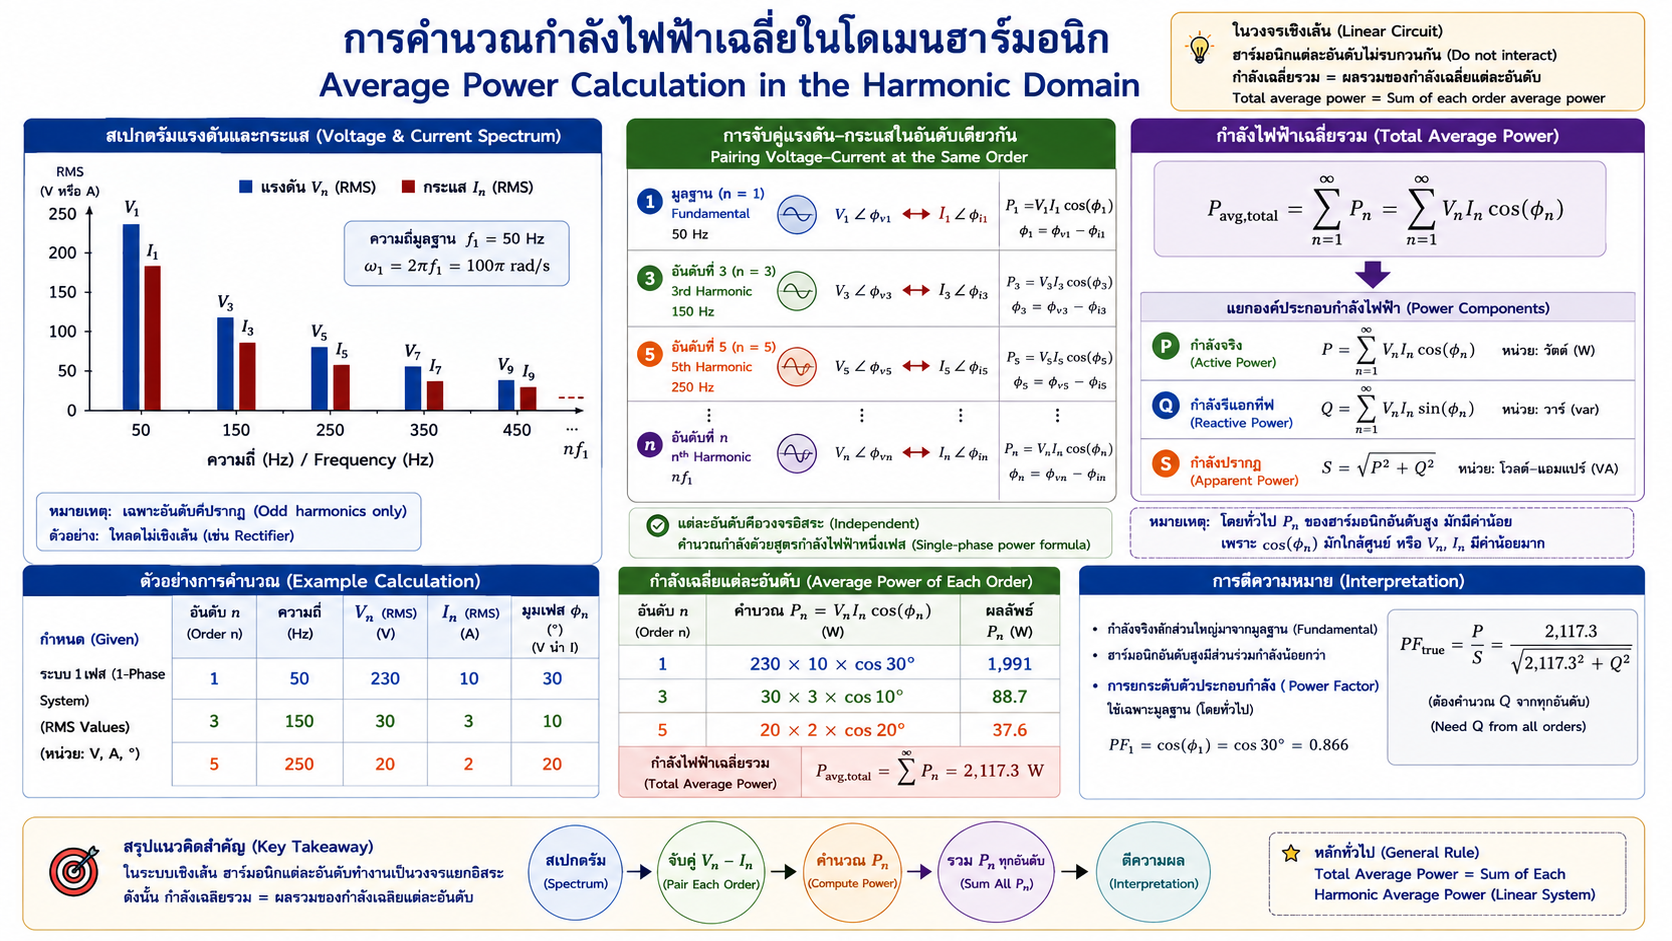
\includegraphics[width=0.8\textwidth]{images/chapter5/figure-05.png}
    \caption{วงจร RC อนุกรมสำหรับกิจกรรมปฏิบัติการที่ 1}
\end{figure}

\textbf{5. ข้อควรระวังด้านความปลอดภัย}

\begin{itemize}
    \item ใช้แรงดันจากเครื่องกำเนิดสัญญาณไม่เกิน 10–15 V เพื่อความปลอดภัยและป้องกันความเสียหายต่ออุปกรณ์
    \item ตรวจสอบขั้วของตัวเก็บประจุแบบมีขั้ว (Electrolytic) ก่อนต่อวงจรทุกครั้ง
    \item ปิดเครื่องกำเนิดสัญญาณก่อนเปลี่ยนค่าตัวต้านทานหรือตัวเก็บประจุทุกครั้ง
    \item ต่อกราวด์ของออสซิลโลสโคปและเครื่องกำเนิดสัญญาณเข้าจุดเดียวกันเสมอ
\end{itemize}

\textbf{6. ขั้นตอนการปฏิบัติ}

\begin{enumerate}
    \item คำนวณค่า τ ทางทฤษฎีล่วงหน้าจากค่า R และ C ที่จะใช้ในแต่ละชุดการทดลอง
    \item ตั้งความถี่ของสัญญาณคลื่นสี่เหลี่ยมให้มีคาบมากกว่า $10\tau$ เพื่อให้เห็นผลตอบสนองครบสมบูรณ์ในแต่ละครึ่งคาบ
    \item ต่อวงจรตามรูปที่ 5 ด้วยค่า R และ C ชุดแรก
    \item ปรับออสซิลโลสโคปให้เห็นสัญญาณ Vin และ Vc พร้อมกันบนหน้าจอ
    \item ใช้เคอร์เซอร์ของออสซิลโลสโคปวัดเวลาที่ Vc มีค่าถึง 63.2\% ของค่าสุดท้าย บันทึกเป็น τ ที่วัดได้
    \item วัดเวลาที่ Vc ถึง 90\% และ 95\% เพิ่มเติมเพื่อตรวจสอบความสอดคล้องกับทฤษฎี
    \item เปลี่ยนค่า R หรือ C ตามชุดข้อมูลที่กำหนด แล้วทำซ้ำขั้นตอนที่ 4–6 จนครบ 3 ชุด
\end{enumerate}

\textbf{7. ตารางบันทึกผล}

\begin{table}[htbp]
    \centering
    \begin{tabular}{llllll}
        \hline
        \textbf{ชุดที่} & \textbf{R (Ω)} & \textbf{C (μF)} & \textbf{τ ทฤษฎี = RC (ms)} & \textbf{τ วัดได้ (ms)} & \textbf{\%ความคลาดเคลื่อน} \\
        \hline
        1 &  &  &  &  &  \\
        2 &  &  &  &  &  \\
        3 &  &  &  &  &  \\
        \hline
    \end{tabular}
\end{table}

\textbf{8. การคำนวณและวิเคราะห์ผล}

คำนวณ \%ความคลาดเคลื่อนจาก $\left|\dfrac{\tau_{\text{ทฤษฎี}}-\tau_{\text{วัดได้}}}{\tau_{\text{ทฤษฎี}}}\right|\times100$ และวิเคราะห์ว่าความคลาดเคลื่อนมีแนวโน้มเพิ่มขึ้นหรือลดลงเมื่อค่า R หรือ C เปลี่ยนแปลงหรือไม่

\textbf{9. การเปรียบเทียบผลจริงกับทฤษฎีหรือแบบจำลอง}

นำค่า τ ที่วัดได้มาพล็อตกราฟ $V_C(t)$ เปรียบเทียบกับกราฟทฤษฎีที่ได้จาก MATLAB (หัวข้อ 7.6) โดยใช้ค่า R, C จริงที่วัดด้วยมัลติมิเตอร์

\textbf{10. คำถามหลังการทดลอง}

\begin{itemize}
    \item ค่า τ ที่วัดได้สอดคล้องกับค่าทางทฤษฎีหรือไม่ หากมีความคลาดเคลื่อน สาเหตุที่เป็นไปได้คืออะไร
    \item หากเพิ่มค่า R เป็นสองเท่าโดยคงค่า C เดิม τ ที่วัดได้ควรเปลี่ยนแปลงอย่างไร ผลการทดลองสอดคล้องกับที่คาดการณ์หรือไม่
    \item เหตุใดจึงต้องตั้งคาบของสัญญาณคลื่นสี่เหลี่ยมให้มากกว่า $10\tau$
\end{itemize}

\textbf{11. เกณฑ์การประเมิน}

ความถูกต้องของการต่อวงจรและการตั้งค่าเครื่องมือ, ความแม่นยำในการอ่านค่าจากออสซิลโลสโคป, ความครบถ้วนของการบันทึกผล, คุณภาพของการวิเคราะห์เปรียบเทียบทฤษฎีกับผลจริง, การตอบคำถามหลังการทดลอง และการปฏิบัติตามข้อควรระวังด้านความปลอดภัย



\subsubsection{กิจกรรมปฏิบัติการที่ 2: การวัดผลตอบสนองชั่วครู่ของวงจร RLC (ระบบอันดับสอง) และการเปรียบเทียบกับ MATLAB}

\textbf{1. วัตถุประสงค์}
เมื่อเสร็จสิ้นกิจกรรมนี้ ผู้เรียนสามารถต่อวงจร RLC อนุกรม ปรับค่า R เพื่อให้เกิดการตอบสนองแบบ Underdamped, Critically Damped และ Overdamped อ่านค่า $t_r$, $t_p$, $\%OS$, $t_s$ จากออสซิลโลสโคป และเปรียบเทียบกับผลการจำลองด้วย MATLAB

\textbf{2. หลักการและทฤษฎีที่เกี่ยวข้อง}
วงจร RLC อนุกรมที่วัดแรงดันคร่อมตัวเก็บประจุมีฟังก์ชันถ่ายโอน

\[
\frac{V_C(s)}{V_{in}(s)} = \frac{1/LC}{s^2+(R/L)s+1/LC}
\]

เทียบกับรูปมาตรฐานในหัวข้อ 7.2 จะได้

\[
\omega_n = \frac{1}{\sqrt{LC}}, \qquad \zeta = \frac{R}{2}\sqrt{\frac{C}{L}}
\]

สังเกตว่า ζ แปรผันตรงกับ R โดยตรง การปรับค่า R จึงเป็นวิธีที่สะดวกที่สุดในการเปลี่ยนลักษณะการหน่วงของวงจรโดยไม่ต้องเปลี่ยน L หรือ C

\textbf{3. อุปกรณ์ เครื่องมือ และซอฟต์แวร์}

\begin{itemize}
    \item เครื่องกำเนิดสัญญาณคลื่นสี่เหลี่ยม 1 เครื่อง
    \item ออสซิลโลสโคป 1 เครื่อง พร้อมสายโพรบ 2 ชุด
    \item กล่องตัวต้านทานปรับค่าได้ (Decade Resistance Box) หรือชุดตัวต้านทานหลายค่า
    \item ตัวเหนี่ยวนำ (Inductor) L = 10 mH จำนวน 1 ตัว
    \item ตัวเก็บประจุ (Capacitor) C = 1 μF จำนวน 1 ตัว
    \item เบรดบอร์ดและสายเชื่อมต่อ
    \item คอมพิวเตอร์ที่ติดตั้ง MATLAB
\end{itemize}

\textbf{4. แผนภาพหรือวงจร}

% [รูปที่ 6: วงจร RLC อนุกรมสำหรับกิจกรรมปฏิบัติการที่ 2]
% ประเภทภาพ: Experimental Setup
% ตำแหน่งที่แนะนำ: หัวข้อ 10 กิจกรรมปฏิบัติการที่ 2 ส่วนที่ 4
% วัตถุประสงค์การเรียนรู้: ให้ผู้เรียนเข้าใจการต่อวงจร RLC อนุกรมและตำแหน่งการวัดที่สอดคล้องกับฟังก์ชันถ่ายโอนอันดับสอง
% คำอธิบายภาพ: วงจรอนุกรมประกอบด้วยเครื่องกำเนิดสัญญาณคลื่นสี่เหลี่ยมต่อผ่านตัวต้านทาน R ตัวเหนี่ยวนำ L และตัวเก็บประจุ C ตามลำดับ ลงกราวด์ ปลายสายโพรบช่อง 1 วัดสัญญาณเข้า ปลายสายโพรบช่อง 2 วัดแรงดันคร่อม C
% องค์ประกอบที่ต้องมี: สัญลักษณ์เครื่องกำเนิดสัญญาณ, R, L, C, จุดกราวด์, ตำแหน่งโพรบ CH1 และ CH2
% ข้อความหรือป้ายกำกับ: "Vin", "R", "L", "C", "Vc", "CH1", "CH2", "GND"
% ภาษาของป้ายกำกับ: ไทยและอังกฤษ
% สัดส่วนภาพ: 4:3
% Image Generation Prompt: Simple series RLC circuit schematic diagram, function generator connected through a resistor, inductor and capacitor in series to ground, oscilloscope probes labeled CH1 at input and CH2 across the capacitor, clean technical schematic style, black lines on white background
% Alt Text: แผนภาพวงจร RLC อนุกรมพร้อมตำแหน่งการวัดด้วยออสซิลโลสโคปสำหรับกิจกรรมปฏิบัติการที่ 2

\begin{figure}[htbp]
    \centering
    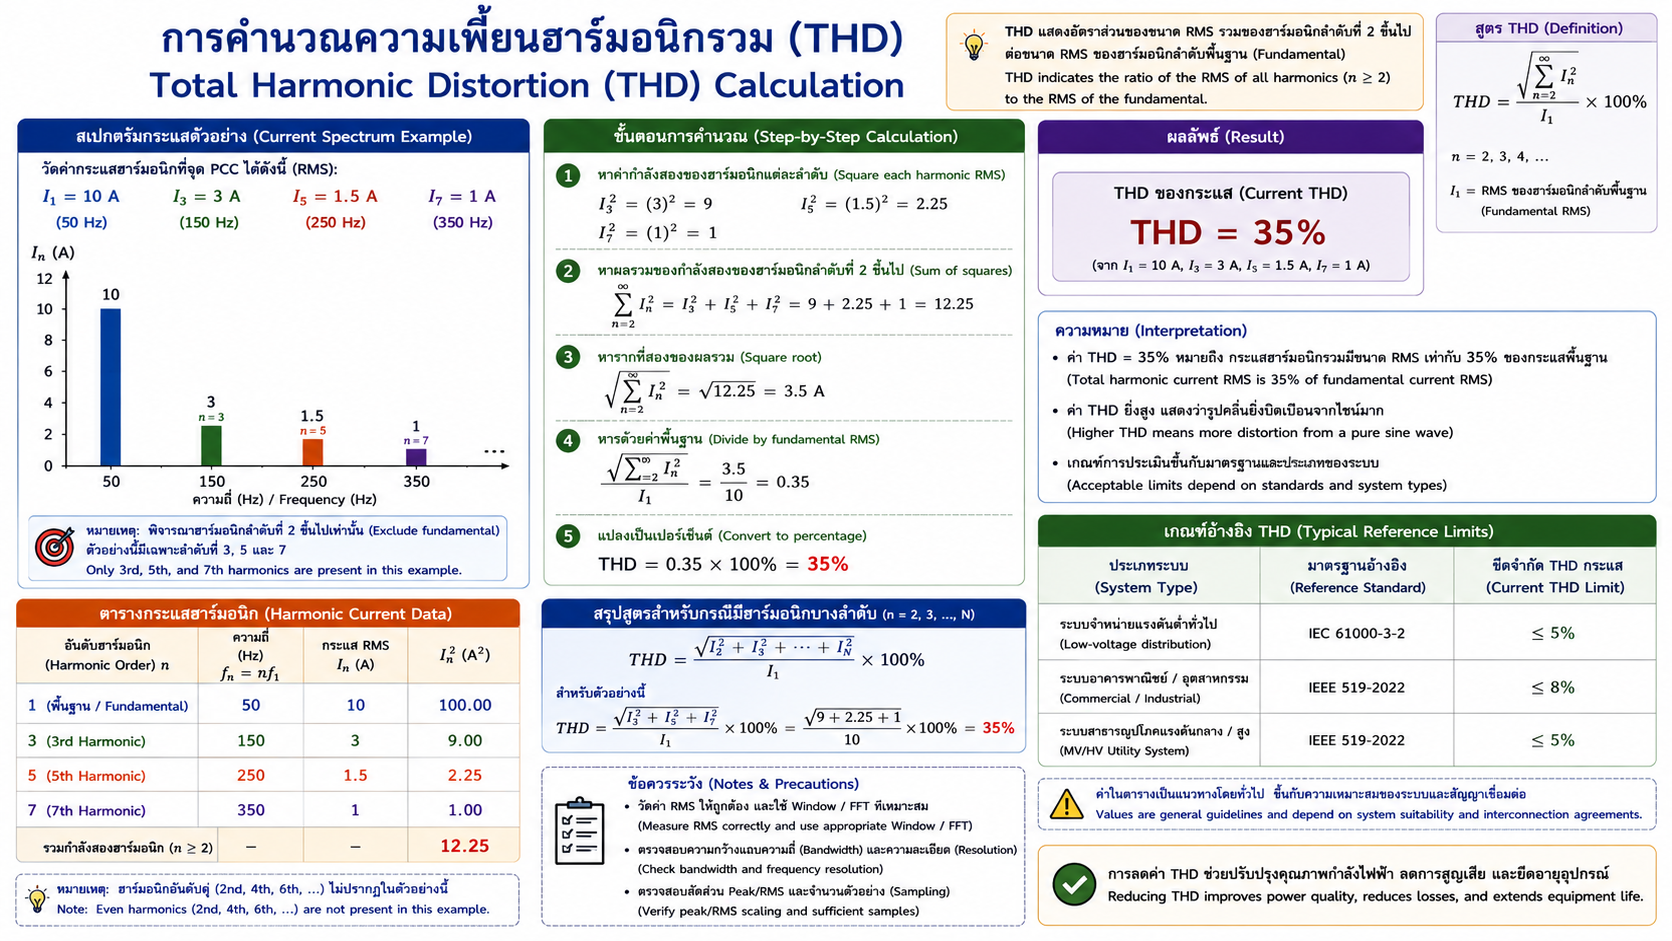
\includegraphics[width=0.8\textwidth]{images/chapter5/figure-06.png}
    \caption{วงจร RLC อนุกรมสำหรับกิจกรรมปฏิบัติการที่ 2}
\end{figure}

\textbf{5. ข้อควรระวังด้านความปลอดภัย}

\begin{itemize}
    \item ตรวจสอบพิกัดกระแสของตัวเหนี่ยวนำก่อนใช้งาน ไม่ให้เกินพิกัดที่ระบุ
    \item ระมัดระวังแรงดันเกิน (Voltage Spike) ที่อาจเกิดขึ้นชั่วขณะเมื่อกระแสผ่านตัวเหนี่ยวนำเปลี่ยนแปลงอย่างรวดเร็ว
    \item ใช้แรงดันจากเครื่องกำเนิดสัญญาณในระดับต่ำ (ไม่เกิน 10–15 V) ตลอดการทดลอง
    \item ต่อกราวด์ของอุปกรณ์ทุกชิ้นเข้าจุดเดียวกันเพื่อลดสัญญาณรบกวน
\end{itemize}

\textbf{6. ขั้นตอนการปฏิบัติ}

\begin{enumerate}
    \item คำนวณค่า $\omega_n=1/\sqrt{LC}$ จาก L=10 mH, C=1 μF ล่วงหน้า
    \item คำนวณค่า R ที่ต้องใช้เพื่อให้ได้ ζ เป้าหมาย 3 ค่า เช่น ζ≈0.3 (Underdamped), ζ=1 (Critically Damped) และ ζ≈2 (Overdamped) จากสูตร $R=2\zeta\sqrt{L/C}$
    \item ต่อวงจรตามรูปที่ 6 ด้วยค่า R ชุดแรก (Underdamped) ตั้งความถี่สัญญาณคลื่นสี่เหลี่ยมให้คาบมากกว่า $10\times t_s$ โดยประมาณ
    \item อ่านค่า $t_r$, $t_p$, $\%OS$, $t_s$ จากหน้าจอออสซิลโลสโคปโดยใช้เคอร์เซอร์วัดเวลาและแรงดัน บันทึกผล
    \item เปลี่ยนค่า R เป็นชุดถัดไป (Critically Damped และ Overdamped) แล้วทำซ้ำขั้นตอนที่ 4 สังเกตการหายไปของการแกว่ง
    \item ในโปรแกรม MATLAB สร้างฟังก์ชันถ่ายโอนด้วยค่า ωn, ζ ที่คำนวณได้ในแต่ละกรณี ใช้คำสั่ง \texttt{step()} และ \texttt{stepinfo()} ตามหัวข้อ 7.6 เพื่อหาค่าทฤษฎี
    \item เปรียบเทียบค่าที่วัดได้จริงกับค่าทฤษฎีจาก MATLAB ในตารางบันทึกผล
\end{enumerate}

\textbf{7. ตารางบันทึกผล}

\begin{table}[htbp]
    \centering
    \small
    \begin{tabularx}{\textwidth}{@{}>{\raggedright\arraybackslash}p{0.14\textwidth}*{7}{>{\centering\arraybackslash}X}@{}}
        \hline
        \textbf{กรณี} & \textbf{R ที่ใช้ (Ω)} & \textbf{ζ คำนวณ} & \textbf{ωn (rad/s)} & \textbf{tr ทฤษฎี/วัดได้ (ms)} & \textbf{tp ทฤษฎี/วัดได้ (ms)} & \textbf{\%OS ทฤษฎี/วัดได้} & \textbf{ts ทฤษฎี/วัดได้ (ms)} \\
        \hline
        Underdamped &  &  &  & / & / & / & / \\
        Critically Damped &  &  &  & / & / & / & / \\
        Overdamped &  &  &  & / & / & / & / \\
        \hline
    \end{tabularx}
\end{table}

\textbf{8. การคำนวณและวิเคราะห์ผล}

คำนวณ \%ความคลาดเคลื่อนของแต่ละตัวชี้วัดระหว่างค่าทฤษฎี (คำนวณด้วยมือหรือจาก MATLAB) กับค่าที่วัดได้จริง วิเคราะห์ว่าตัวชี้วัดใดมีความคลาดเคลื่อนมากที่สุดและเพราะเหตุใด

\textbf{9. การเปรียบเทียบผลจริงกับทฤษฎีหรือแบบจำลอง}

นำภาพหน้าจอออสซิลโลสโคป (หรือข้อมูลที่บันทึกได้) มาซ้อนทับกับกราฟที่ได้จาก MATLAB ในหัวข้อ 7.6 เพื่อเปรียบเทียบรูปร่างของกราฟโดยตรง

\textbf{10. คำถามหลังการทดลอง}

\begin{itemize}
    \item เมื่อเพิ่มค่า R ขึ้นเรื่อย ๆ ลักษณะของผลตอบสนองเปลี่ยนแปลงอย่างไร และสอดคล้องกับทฤษฎีในหัวข้อ 7.3 หรือไม่
    \item เหตุใดกรณี Critically Damped จึงไม่มีการพุ่งเกินค่าสุดท้ายเลย
    \item ระบุแหล่งที่มาของความคลาดเคลื่อนระหว่างผลการทดลองกับทฤษฎีที่พบในกิจกรรมนี้อย่างน้อย 2 แหล่ง (เช่น ความต้านทานปรสิตในตัวเหนี่ยวนำ ความคลาดเคลื่อนของพิกัดอุปกรณ์ หรือผลจากโพรบวัด)
\end{itemize}

\textbf{11. เกณฑ์การประเมิน}

ความถูกต้องของการคำนวณค่า R ล่วงหน้า, ความถูกต้องของการต่อวงจรและปรับค่า R, ความแม่นยำในการอ่านค่าจากออสซิลโลสโคป, ความถูกต้องของการจำลองด้วย MATLAB, คุณภาพของการวิเคราะห์เปรียบเทียบ, การตอบคำถามหลังการทดลอง และการปฏิบัติตามข้อควรระวังด้านความปลอดภัย

\newpage

\subsection{11. สรุปท้ายบท}

บทนี้ได้อธิบายการวิเคราะห์ผลตอบสนองชั่วครู่ของระบบควบคุมและข้อกำหนดสมรรถนะที่ใช้ในการออกแบบ สรุปสาระสำคัญได้ดังนี้

\begin{itemize}
    \item \textbf{ระบบอันดับหนึ่ง} อธิบายด้วยค่าคงเวลา τ เพียงตัวเดียว ผลตอบสนองต่อสัญญาณขั้นบันไดคือ $c(t)=1-e^{-t/\tau}$ โดยถึง 63.2\% ที่ $t=\tau$ และเข้าใกล้ค่าสุดท้ายภายในประมาณ $4\tau$–$5\tau$
    \item \textbf{ระบบอันดับสอง} อธิบายด้วยพารามิเตอร์สองตัวคือ ζ (อัตราส่วนหน่วง) และ ωn (ความถี่ธรรมชาติ) ในรูปมาตรฐาน $\omega_n^2/(s^2+2\zeta\omega_n s+\omega_n^2)$
    \item ประเภทของการตอบสนองแบ่งตามค่า ζ ได้แก่ Undamped ($\zeta=0$), Underdamped ($0<\zeta<1$), Critically Damped ($\zeta=1$) และ Overdamped ($\zeta>1$) ซึ่งสัมพันธ์โดยตรงกับตำแหน่งโพลบนระนาบ s
    \item ข้อกำหนดสมรรถนะหลักสี่ค่าสำหรับกรณี Underdamped ได้แก่ Rise Time ($t_r\approx1.8/\omega_n$), Peak Time ($t_p=\pi/\omega_d$), Percent Overshoot ($\%OS=e^{-\zeta\pi/\sqrt{1-\zeta^2}}\times100$) และ Settling Time ($t_s\approx4/(\zeta\omega_n)$ ที่เกณฑ์ 2\%)
    \item \textbf{\%OS ขึ้นกับ ζ เพียงตัวเดียว} ทำให้สามารถแก้สมการย้อนกลับหา ζ ที่ต้องการจากข้อกำหนดการออกแบบได้โดยตรง
    \item \textbf{ความผิดพลาดคงตัว} คำนวณด้วยทฤษฎีบทค่าสุดท้าย และสัมพันธ์กับ \textbf{System Type} (จำนวนโพลของวงเปิดที่ $s=0$) ผ่านค่าคงที่ความผิดพลาด $K_p$, $K_v$, $K_a$
    \item สมมติฐานสำคัญคือสูตรทั้งหมดอ้างอิงระบบอันดับสองมาตรฐานที่ไม่มีซีโรหรือโพลเพิ่มเติมใกล้คู่โพลหลัก และต้องระบุเกณฑ์ Settling Time (2\% หรือ 5\%) กำกับเสมอ
    \item ค่าที่คำนวณด้วยมือควรตรวจสอบด้วยการจำลองใน MATLAB ผ่านคำสั่ง \texttt{step()} และ \texttt{stepinfo()} และเปรียบเทียบกับผลการวัดจริงจากวงจร RC และ RLC
\end{itemize}



\subsection{12. คำถามทบทวน}

\begin{enumerate}
    \item จงอธิบายความแตกต่างระหว่างผลตอบสนองชั่วครู่ (Transient Response) และผลตอบสนองคงตัว (Steady-State Response)
    \item ค่าคงเวลา (τ) ของระบบอันดับหนึ่งมีความหมายทางกายภาพอย่างไร และสัมพันธ์กับความเร็วในการตอบสนองของระบบอย่างไร
    \item จงเปรียบเทียบลักษณะของการตอบสนองแบบ Underdamped, Critically Damped และ Overdamped ทั้งในรูปแบบสมการคำตอบและตำแหน่งโพลบนระนาบ s
    \item เหตุใด Percent Overshoot (\%OS) จึงขึ้นอยู่กับอัตราส่วนหน่วง (ζ) เพียงอย่างเดียว โดยไม่ขึ้นกับค่าความถี่ธรรมชาติ (ωn)
    \item Settling Time และ Peak Time แตกต่างกันอย่างไร แต่ละค่าสัมพันธ์กับพารามิเตอร์ใดของระบบอันดับสอง
    \item System Type คืออะไร และมีความสัมพันธ์อย่างไรกับจำนวนตัวรวมสัญญาณ (Integrator) ในฟังก์ชันถ่ายโอนวงเปิด
    \item จงอธิบายว่าเหตุใดระบบชนิดที่ 1 (Type 1) จึงมีความผิดพลาดคงตัวเป็นศูนย์สำหรับสัญญาณขั้นบันได แต่มีค่าความผิดพลาดคงตัวจำกัดสำหรับสัญญาณทางลาด (Ramp)
    \item หากต้องการออกแบบระบบให้มี \%OS ต่ำและ Settling Time สั้น มีข้อจำกัดหรือข้อพิจารณาใดที่วิศวกรต้องคำนึงถึง
\end{enumerate}

\newpage

\subsection{13. แบบฝึกหัดท้ายบท}

เฉลยละเอียดของแบบฝึกหัดทั้งหมดอยู่ในหัวข้อที่ 14 (สำหรับผู้สอน) หากต้องการแจกเป็นเอกสารสำหรับนักศึกษาโดยไม่เปิดเผยคำตอบ ให้คัดลอกเฉพาะหัวข้อนี้แยกออกไปเป็นเอกสารต่างหาก

\subsubsection{ระดับพื้นฐาน}

\textbf{ข้อ B1.} ระบบวงปิดมีฟังก์ชันถ่ายโอน $G(s)=\dfrac{8}{s+8}$ จงหาค่าคงเวลา τ และเวลาที่ผลตอบสนองต่อสัญญาณขั้นบันไดหนึ่งหน่วยมีค่าถึง 95\% ของค่าสุดท้าย

\textbf{ข้อ B2.} ระบบอันดับสองมีค่า $\omega_n=10$ rad/s และ $\zeta=1.5$ จงระบุประเภทของการตอบสนอง พร้อมให้เหตุผลประกอบ

\textbf{ข้อ B3.} ระบบวงปิดมีฟังก์ชันถ่ายโอน $T(s)=\dfrac{25}{s^2+10s+25}$ จงหาค่า $\omega_n$ และ $\zeta$ พร้อมระบุประเภทของการตอบสนอง

\textbf{ข้อ B4.} จงพิสูจน์ (หรือแสดงการคำนวณ) ว่าที่เวลา $t=\tau$ ผลตอบสนองของระบบอันดับหนึ่งต่อสัญญาณขั้นบันไดหนึ่งหน่วยมีค่าเท่ากับ 63.2\% ของค่าสุดท้ายเสมอ ไม่ว่าค่า τ จะเป็นเท่าใด

\textbf{ข้อ B5.} ระบบป้อนกลับหนึ่งหน่วยมีฟังก์ชันถ่ายโอนวงเปิด $G(s)=\dfrac{50}{s(s+2)(s+10)}$ จงหาว่าระบบนี้เป็น System Type ใด

\subsubsection{ระดับวิเคราะห์}

\textbf{ข้อ A1.} ระบบวงปิดมีฟังก์ชันถ่ายโอน $T(s)=\dfrac{64}{s^2+6.4s+64}$ จงคำนวณ $t_p$, $\%OS$ และ $t_s$ (เกณฑ์ 2\%)

\textbf{ข้อ A2.} ต้องการออกแบบระบบให้มี $\%OS \le 10\%$ (ก) จงหาค่า ζ ต่ำสุดที่ต้องใช้ (ข) หากต้องการให้ $t_s \le 1.5$ วินาที (เกณฑ์ 2\%) โดยใช้ค่า ζ จากข้อ (ก) จงหาค่า $\omega_n$ ต่ำสุดที่ต้องใช้

\textbf{ข้อ A3.} ระบบอันดับสองสองระบบมี $\omega_n=5$ rad/s เท่ากัน แต่มี $\zeta_1=0.2$ และ $\zeta_2=0.8$ จงคำนวณ $t_p$, $\%OS$ และ $t_s$ (เกณฑ์ 2\%) ของทั้งสองระบบ แล้วอธิบายแนวโน้มที่พบ พร้อมอธิบายเชิงกายภาพว่าเหตุใดจึงเป็นเช่นนั้น

\textbf{ข้อ A4.} ระบบป้อนกลับหนึ่งหน่วยมีฟังก์ชันถ่ายโอนวงเปิด $G(s)=\dfrac{100}{s(s+10)}$ จงหาค่า $K_p$, $K_v$, $K_a$ และความผิดพลาดคงตัวเมื่อป้อนสัญญาณทางลาด $r(t)=3t$

\textbf{ข้อ A5.} ระบบป้อนกลับหนึ่งหน่วยมีฟังก์ชันถ่ายโอนวงเปิด $G(s)=\dfrac{K}{(s+2)(s+5)}$ จงหาค่า K ต่ำสุดที่ทำให้ความผิดพลาดคงตัวต่อสัญญาณขั้นบันไดหนึ่งหน่วยไม่เกิน 5\%

\subsubsection{ระดับประยุกต์ใช้}

\textbf{ข้อ AP1.} ระบบควบคุมความเร็วมอเตอร์มีฟังก์ชันถ่ายโอนวงเปิด $G(s)=\dfrac{K}{s(s+8)}$ ต่อแบบป้อนกลับหนึ่งหน่วย ข้อกำหนดของงานต้องการ $\%OS \le 20\%$ และ $t_s \le 2.5$ วินาที (เกณฑ์ 2\%) โดยพิจารณาเฉพาะกรณี Underdamped จงหาช่วงค่า K ที่เป็นไปได้

\textbf{ข้อ AP2.} วงจร RLC อนุกรมมีค่า $L=10$ mH และ $C=1$ μF ต้องการออกแบบให้ระบบมีลักษณะ Critically Damped ($\zeta=1$) (ก) จงหาค่าความต้านทาน R ที่ต้องใช้ (ข) หากต้องการปรับให้ระบบมี $\zeta=0.5$ (Underdamped) แทน ค่า R ควรเป็นเท่าใด และระบบที่ได้จะมี \%OS เท่าใด

\textbf{ข้อ AP3.} ระบบลิฟต์โดยสารต้องเคลื่อนที่ด้วยความเร็วคงที่ในบางช่วง (สัญญาณอ้างอิงแบบทางลาด) (ก) ระบบควบคุมต้องมี System Type อย่างน้อยเท่าใดจึงจะมีความผิดพลาดคงตัวเป็นศูนย์สำหรับสัญญาณทางลาด (ข) หากระบบที่ใช้จริงมีฟังก์ชันถ่ายโอนวงเปิด $G(s)=\dfrac{K}{s(s+10)}$ (Type 1) ซึ่งไม่สามารถทำให้ความผิดพลาดเป็นศูนย์ได้ จงหาค่า K ต่ำสุดที่ทำให้ความผิดพลาดคงตัวต่อสัญญาณทางลาดหนึ่งหน่วยไม่เกิน 2\%

\newpage

\subsection{14. เฉลยแบบฝึกหัด (สำหรับผู้สอน)}

\subsubsection{ระดับพื้นฐาน}

\textbf{เฉลยข้อ B1}
แนวคิด/หลักการ: จัดรูป $G(s)$ ให้อยู่ในรูปมาตรฐาน $K/(\tau s+1)$ แล้วใช้ $c(t)=1-e^{-t/\tau}$

\[
G(s)=\frac{8}{s+8}=\frac{1}{0.125s+1} \;\Rightarrow\; \tau=0.125 \text{ s}
\]

\[
t_{95\%} = \tau\ln(20) = 0.125\times2.9957 = 0.3745 \text{ s} \approx 374.5 \text{ ms}
\]

คำตอบ: τ = 0.125 s, $t_{95\%}\approx374.5$ ms — ระบบนี้ตอบสนองเร็ว เข้าใกล้ค่าสุดท้ายภายในเวลาต่ำกว่าครึ่งวินาที
ข้อผิดพลาดที่พบบ่อย: ลืมหารทั้งเศษและส่วนด้วยสัมประสิทธิ์ของ s ก่อนอ่านค่า τ ทำให้ได้ τ=1 แทนที่จะเป็น 0.125

\textbf{เฉลยข้อ B2}
แนวคิด/หลักการ: เกณฑ์การจำแนกประเภทจากค่า ζ
เนื่องจาก $\zeta=1.5>1$ ระบบจึงเป็น \textbf{Overdamped}
เหตุผลประกอบ: ค่า ωn ไม่มีผลต่อการจำแนกประเภท มีเพียงค่า ζ เท่านั้นที่กำหนดประเภทของการตอบสนอง

\textbf{เฉลยข้อ B3}
แนวคิด/หลักการ: เทียบสัมประสิทธิ์กับรูปมาตรฐาน

\[
\omega_n^2=25\Rightarrow\omega_n=5 \text{ rad/s}, \qquad 2\zeta\omega_n=10\Rightarrow\zeta=1
\]

คำตอบ: $\omega_n=5$ rad/s, $\zeta=1$ → \textbf{Critically Damped}
ข้อผิดพลาดที่พบบ่อย: สับสนเครื่องหมายหรือลืมหารด้วย 2 เมื่อหา ζ จากสัมประสิทธิ์ของ s

\textbf{เฉลยข้อ B4}
แนวคิด/หลักการ: แทน $t=\tau$ ลงในสมการ $c(t)=1-e^{-t/\tau}$ โดยตรง

\[
c(\tau) = 1-e^{-\tau/\tau} = 1-e^{-1} = 1-0.3679 = 0.6321
\]

คำตอบ: 63.2\% การแปลความหมาย: อัตราส่วน $t/\tau=1$ เสมอเมื่อ $t=\tau$ ไม่ว่าค่า τ จริงจะเป็นเท่าใด ผลลัพธ์ $e^{-1}$ จึงคงที่เสมอ นี่คือเหตุผลที่ 63.2\% เป็นค่าคงที่สากลสำหรับระบบอันดับหนึ่งทุกระบบ

\textbf{เฉลยข้อ B5}
แนวคิด/หลักการ: นับจำนวนโพลที่ $s=0$ ของฟังก์ชันถ่ายโอนวงเปิด
$G(s)$ มีตัวประกอบ $s$ หนึ่งตัวในตัวส่วน (ไม่นับ $(s+2)$ และ $(s+10)$ ซึ่งเป็นโพลที่ตำแหน่งอื่น) ดังนั้นเป็น \textbf{System Type 1}

\subsubsection{ระดับวิเคราะห์}

\textbf{เฉลยข้อ A1}
แนวคิด/หลักการ: เทียบสัมประสิทธิ์หา ζ, ωn แล้วแทนในสูตรข้อกำหนดสมรรถนะ

\[
\omega_n=8 \text{ rad/s}, \quad \zeta=\frac{6.4}{16}=0.4, \quad \omega_d=8\sqrt{1-0.16}=7.332 \text{ rad/s}
\]

\begin{align*}
t_p &= \frac{\pi}{7.332}=0.428 \text{ s},\\
\%OS &= e^{-0.4\pi/\sqrt{0.84}}\times100=25.4\%,\\
t_s &= \frac{4}{0.4\times8}=1.25 \text{ s}
\end{align*}

คำตอบ: $t_p\approx0.428$ s, $\%OS\approx25.4\%$, $t_s=1.25$ s (เกณฑ์ 2\%)

\textbf{เฉลยข้อ A2}
แนวคิด/หลักการ: ใช้สูตรผกผันของ \%OS หา ζ ก่อน แล้วจึงใช้สูตร $t_s$ หา ωn

(ก)
\[
\zeta_{min}=\frac{-\ln(0.10)}{\sqrt{\pi^2+\ln^2(0.10)}}=\frac{2.3026}{\sqrt{9.8696+5.3019}}=\frac{2.3026}{3.8951}=0.591
\]

(ข)
\[
t_s=\frac{4}{\zeta\omega_n}\le1.5 \;\Rightarrow\; \omega_n\ge\frac{4}{1.5\times0.591}=4.51 \text{ rad/s}
\]

คำตอบ: (ก) $\zeta\ge0.591$ (ข) $\omega_n\ge4.51$ rad/s
การแปลความหมาย: ต้องเลือกทั้ง ζ และ ωn ให้อยู่ในช่วงที่คำนวณได้พร้อมกัน จึงจะสอดคล้องกับข้อกำหนดทั้งสองข้อ

\textbf{เฉลยข้อ A3}
แนวคิด/หลักการ: แทนค่าลงในสูตร $t_p$, $\%OS$, $t_s$ สำหรับแต่ละกรณีที่ ωn=5 คงที่

กรณี $\zeta_1=0.2$: $\omega_d=4.899$ rad/s, $t_{p1}=0.641$ s, $\%OS_1=52.7\%$, $t_{s1}=4.0$ s
กรณี $\zeta_2=0.8$: $\omega_d=3.0$ rad/s, $t_{p2}=1.047$ s, $\%OS_2=1.52\%$, $t_{s2}=1.0$ s

การแปลความหมาย/เหตุผลประกอบ: เมื่อ ζ เพิ่มขึ้นโดย ωn คงที่ ส่วนจริงของโพล ($\zeta\omega_n$) จะเพิ่มขึ้นตามสัดส่วน ทำให้เปลือกเลขชี้กำลังของผลตอบสนองสลายตัวเร็วขึ้น จึงได้ Settling Time ที่สั้นลง ในขณะที่ส่วนจินตภาพของโพล ($\omega_d$) ลดลง ทำให้คาบการแกว่งยาวขึ้นและ Peak Time เพิ่มขึ้น ส่วน \%OS ลดลงอย่างมากเพราะความหน่วงที่มากขึ้นไปหน่วงขนาดของการแกว่งโดยตรง สำหรับ Rise Time แนวโน้มคือเพิ่มขึ้นตาม ζ เช่นกัน (ระบบขึ้นถึงค่าสุดท้ายช้าลง) แม้สูตรประมาณ $t_r\approx1.8/\omega_n$ จะไม่แสดงความสัมพันธ์กับ ζ อย่างชัดเจน ค่าที่แม่นยำต้องหาด้วยวิธีเชิงตัวเลขหรือ MATLAB

\textbf{เฉลยข้อ A4}
แนวคิด/หลักการ: หา $K_v$ จากนิยาม แล้วใช้ $e_{ss}=A/K_v$ สำหรับสัญญาณ $r(t)=At$

\[
K_v=\lim_{s\to0}s\cdot\frac{100}{s(s+10)}=\frac{100}{10}=10
\]

\[
e_{ss}=\frac{3}{K_v}=\frac{3}{10}=0.3
\]

คำตอบ: $K_p\to\infty$, $K_v=10$, $K_a=0$, $e_{ss}=0.3$ (สำหรับ $r(t)=3t$)

\textbf{เฉลยข้อ A5}
แนวคิด/หลักการ: ระบบเป็น Type 0 ใช้ $K_p$ และสูตร $e_{ss}=1/(1+K_p)$

\[
K_p=\lim_{s\to0}\frac{K}{(s+2)(s+5)}=\frac{K}{10}
\]

\[
e_{ss}=\frac{1}{1+K/10}=\frac{10}{10+K}\le0.05
\]

\[
10\le0.05(10+K) \;\Rightarrow\; K\ge190
\]

คำตอบ: $K_{min}=190$

\subsubsection{ระดับประยุกต์ใช้}

\textbf{เฉลยข้อ AP1}
แนวคิด/หลักการ: เช่นเดียวกับตัวอย่างที่ 4 หา ζ ต่ำสุดจาก \%OS ก่อน แล้วใช้ความสัมพันธ์ $\zeta\omega_n=$ คงที่ หาช่วง K

\[
T(s)=\frac{K}{s^2+8s+K} \;\Rightarrow\; \zeta\omega_n=4 \text{ (คงที่)}
\]

\[
\zeta_{min}=\frac{-\ln(0.2)}{\sqrt{\pi^2+\ln^2(0.2)}}=\frac{1.6094}{3.5299}=0.456
\]

\[
\omega_n\le\frac{4}{0.456}=8.77 \text{ rad/s} \;\Rightarrow\; K\le76.9
\]

เงื่อนไข Underdamped: $\zeta<1\Rightarrow\omega_n>4\Rightarrow K>16$

ตรวจสอบ ts: $t_s=4/(\zeta\omega_n)=4/4=1.0$ s ซึ่งน้อยกว่า 2.5 s เสมอในช่วงนี้

คำตอบ: $16 < K \le 76.9$

\textbf{เฉลยข้อ AP2}
แนวคิด/หลักการ: ใช้ $\zeta=(R/2)\sqrt{C/L}$ ของวงจร RLC อนุกรม แก้หา R

\[
\sqrt{\frac{L}{C}}=\sqrt{\frac{0.01}{0.000001}}=\sqrt{10000}=100 \;\Omega
\]

(ก) $\zeta=1$: $R=2\times1\times100=200\;\Omega$

(ข) $\zeta=0.5$: $R=2\times0.5\times100=100\;\Omega$

\[
\%OS=e^{-0.5\pi/\sqrt{1-0.25}}\times100=e^{-1.814}\times100=16.3\%
\]

คำตอบ: (ก) R = 200 Ω (ข) R = 100 Ω, \%OS ≈ 16.3\%

\textbf{เฉลยข้อ AP3}
แนวคิด/หลักการ: (ก) ใช้หลักการ System Type กับสัญญาณทางลาด (ข) ใช้ $K_v$ ของระบบ Type 1

(ก) ต้องมี System Type ≥ 2 จึงจะได้ $e_{ss}(\text{ramp})=0$

(ข)
\[
K_v=\lim_{s\to0}s\cdot\frac{K}{s(s+10)}=\frac{K}{10}, \qquad e_{ss}=\frac{1}{K_v}=\frac{10}{K}\le0.02
\]

\[
K\ge500
\]

คำตอบ: (ก) System Type 2 (ข) $K_{min}=500$
การแปลความหมาย: หากไม่สามารถเปลี่ยนโครงสร้างระบบให้เป็น Type 2 ได้ วิศวกรยังสามารถลดความผิดพลาดคงตัวให้อยู่ในเกณฑ์ที่ยอมรับได้ด้วยการเพิ่มอัตราขยายวงเปิดให้เพียงพอ แม้จะไม่สามารถทำให้ความผิดพลาดเป็นศูนย์สมบูรณ์ได้



\subsection{15. ข้อเสนอแนะสำหรับผู้สอน}

\textbf{ลำดับการสอนที่แนะนำ:} เริ่มจากระบบอันดับหนึ่ง (7.1) ซึ่งมีพารามิเตอร์เดียวและเข้าใจง่ายกว่า ก่อนขยายไปสู่ระบบอันดับสอง (7.2–7.5) ควรใช้เวลาเน้นย้ำหัวข้อ 7.3–7.4 มากที่สุด เนื่องจากเป็นแกนหลักของบทและเป็นฐานสำหรับการออกแบบตัวควบคุมในบทถัดไป หัวข้อ 7.6 (MATLAB) ควรสอนแทรกหลังหัวข้อ 7.4 ทันที เพื่อให้นักศึกษาได้ตรวจสอบผลการคำนวณด้วยมือทันทีที่เรียนสูตร

\textbf{จุดที่ผู้เรียนมักมีปัญหา:}

\begin{itemize}
    \item การแยกแยะ ωn กับ ωd และการเข้าใจว่าค่าใดคือความถี่ที่สังเกตเห็นได้จริง
    \item การจดจำและใช้สูตร \%OS-ζ ผิดทิศทาง (คิดว่า ζ สูงทำให้ \%OS สูง)
    \item ความสับสนระหว่าง System Type และ System Order ตามที่ระบุในหัวข้อ 8
    \item การลืมระบุเกณฑ์ Settling Time (2\% หรือ 5\%) กำกับคำตอบ
\end{itemize}

\textbf{สำหรับนักศึกษาสายสามัญ (ม.6):} แนะนำให้เริ่มจากการฝึก\textbf{อ่านค่าจากกราฟ}ก่อนเข้าสู่สูตรคำนวณ โดยใช้รูปที่ 4 เป็นสื่อหลัก ให้นักศึกษาฝึกชี้ตำแหน่ง tr, tp, \%OS, ts บนกราฟตัวอย่างหลายแบบ จนคุ้นเคยกับความหมายเชิงภาพก่อน จึงค่อยเชื่อมโยงเข้ากับสูตรคำนวณในภายหลัง วิธีนี้ช่วยลดความรู้สึกว่าเนื้อหาเป็นนามธรรมเกินไป

\textbf{สำหรับนักศึกษาสายอาชีวศึกษา (ปวช.):} แนะนำให้เชื่อมโยงแนวคิด Overshoot และ Settling Time เข้ากับประสบการณ์จริงที่เกี่ยวข้องกับมอเตอร์หรือระบบขับเคลื่อน เช่น การกระชากของมอเตอร์เมื่อเปิดสวิตช์ทันที หรือการแกว่งของสายพานลำเลียงเมื่อเริ่มเดินเครื่อง เพื่อสร้างความเชื่อมโยงระหว่างทฤษฎีกับประสบการณ์ปฏิบัติที่มีอยู่แล้ว

\textbf{แนวทางประเมินระหว่างเรียน:} ใช้กิจกรรม Think-Pair-Share ให้นักศึกษาจับคู่อ่านค่าจากกราฟผลตอบสนองก่อนสรุปเป็นชั้นเรียน และใช้ Exit Ticket ท้ายคาบให้คำนวณค่าพารามิเตอร์อย่างง่าย (เช่น หา ζ, ωn จากฟังก์ชันถ่ายโอนที่กำหนด) เพื่อตรวจสอบความเข้าใจก่อนเข้าสู่หัวข้อถัดไป



\subsection{16. สื่อและแหล่งเรียนรู้เพิ่มเติม}

\begin{table}[htbp]
    \centering
    \small
    \begin{tabularx}{\textwidth}{@{}>{\raggedright\arraybackslash}p{0.14\textwidth}*{4}{>{\raggedright\arraybackslash}X}@{}}
        \hline
        \textbf{แหล่ง/องค์กร} & \textbf{หัวข้อที่ควรค้น} & \textbf{คำค้นแนะนำ} & \textbf{จุดประสงค์ในการรับชม} & \textbf{ช่วงเวลาที่เหมาะสม} \\
        \hline
        NPTEL & Time Response Analysis & "NPTEL Time Response Analysis Control Systems" & เสริมความเข้าใจการวิเคราะห์ผลตอบสนองเชิงเวลาอย่างเป็นระบบและละเอียด & หลังเรียนหัวข้อ 7.1–7.2 ก่อนเข้าสู่หัวข้อ 7.3 \\
        MathWorks & Step Response and Control System Performance & "MathWorks Step Response Control System Performance" & แสดงการใช้งาน MATLAB คำสั่ง \texttt{step()} และ \texttt{stepinfo()} ประกอบการคำนวณด้วยมือ & ช่วงสอนหัวข้อ 7.6 หรือก่อนเข้าห้องปฏิบัติการที่ 2 \\
        \hline
    \end{tabularx}
\end{table}

\textbf{คำค้นเพิ่มเติมที่แนะนำสำหรับการค้นคว้าด้วยตนเอง:} "Transient Response Control Systems", "Second Order System Overshoot Settling Time", "Step Response MATLAB"

หมายเหตุ: รายการข้างต้นเป็นแนวทางค้นหาตามชื่อองค์กรและหัวข้อที่ผู้สอนกำหนด ยังไม่ได้ระบุลิงก์ ชื่อคลิป ผู้บรรยาย หรือปีเผยแพร่เฉพาะเจาะจง ผู้สอนควรค้นหาและตรวจสอบคลิปที่เหมาะสมกับเนื้อหาก่อนใช้งานจริงในชั้นเรียน



\subsection{17. เอกสารอ้างอิง}

\subsubsection{หนังสือและตำรา}

\begin{enumerate}
    \item Nise, N. S. (2019). \textit{Control Systems Engineering} (8th ed.). Wiley.
    \item Ogata, K. (2010). \textit{Modern Control Engineering} (5th ed.). Pearson.
    \item Dorf, R. C., \& Bishop, R. H. (2016). \textit{Modern Control Systems} (13th ed.). Pearson.
\end{enumerate}

\subsubsection{เอกสารทางเทคนิคและคู่มือซอฟต์แวร์}

\begin{enumerate}
    \item MathWorks. \textit{Control System Toolbox Documentation: step, stepinfo.} เว็บไซต์ทางการของ MathWorks
\end{enumerate}

\textbf{หมายเหตุสำหรับผู้สอน:} รายการที่ 1–3 เป็นตำราหลักที่ใช้อ้างอิงเนื้อหาและสัญกรณ์มาตรฐานตลอดบทนี้ ผู้สอนควรตรวจสอบเลขฉบับพิมพ์และรายละเอียดบรรณานุกรมให้ตรงกับฉบับที่มีในห้องสมุดหรือที่ใช้อ้างอิงจริงก่อนเผยแพร่เอกสารนี้อย่างเป็นทางการ และรายการที่ 4 ควรระบุ URL ที่เข้าถึงได้จริงในขณะที่จัดทำเอกสารฉบับเผยแพร่



\textbf{ข้อมูลความยาวเป้าหมายและเวลาสอนที่รองรับ:} เอกสารฉบับนี้จัดทำสำหรับการสอนบรรยาย 6 ชั่วโมง ความยาวเนื้อหาหลัก (หัวข้อ 1–12) อยู่ในกรอบเป้าหมายไม่เกิน 25–30 หน้า A4 ตามข้อกำหนด ส่วนหัวข้อ 13–17 (แบบฝึกหัด เฉลยสำหรับผู้สอน ข้อเสนอแนะการสอน สื่อ และเอกสารอ้างอิง) เป็นส่วนเสริมสำหรับผู้สอนตามหลักการควบคุมความยาวในข้อ 5.4 ของ Prompt กลาง

\section{บทที่ 5 การประยุกต์อนุกรมฟูเรียร์ในการวิเคราะห์รูปคลื่นไฟฟ้า}

\textbf{ชื่อบทภาษาอังกฤษ:} Applications of Fourier Series in Electrical Waveform Analysis \\
\textbf{รายวิชา:} 5571102 คณิตศาสตร์วิศวกรรมไฟฟ้า (Electrical Engineering Mathematics) \\
\textbf{สาขาวิชา:} เทคโนโลยีวิศวกรรมไฟฟ้า



\subsection{1. แนวคิดสำคัญของบท}

บทที่ 4 ได้วางพื้นฐานว่า \textbf{ฟังก์ชันเป็นคาบ (periodic function)} ที่มีรูปคลื่นไม่เป็นไซน์สามารถเขียนเป็นผลรวมขององค์ประกอบไซน์และโคไซน์ที่มีความถี่เป็นจำนวนเต็มเท่าของความถี่มูลฐานได้ แนวคิดดังกล่าวเป็นหัวใจของ \textbf{อนุกรมฟูเรียร์ (Fourier series)} และเป็นสะพานเชื่อมจากคณิตศาสตร์ไปสู่การวิเคราะห์สัญญาณและระบบไฟฟ้าในโลกจริง

ในบทนี้จะนำอนุกรมฟูเรียร์มาใช้ตอบคำถามทางวิศวกรรมที่สำคัญ เช่น

\begin{itemize}
    \item เหตุใดกระแสของโหลดอิเล็กทรอนิกส์บางชนิดจึงมีรูปคลื่นไม่เป็นไซน์ แม้แรงดันจ่ายจะใกล้เคียงไซน์
    \item รูปคลื่นสี่เหลี่ยม สามเหลี่ยม และฟันเลื่อยประกอบด้วยฮาร์มอนิกลำดับใดบ้าง และแอมพลิจูดลดลงเร็วเพียงใด
    \item ค่าประสิทธิผลหรือ RMS ของรูปคลื่นไม่เป็นไซน์ควรคำนวณอย่างไร
    \item เมื่อแรงดันและกระแสมีฮาร์มอนิก กำลังไฟฟ้าเฉลี่ยและตัวประกอบกำลังควรตีความอย่างไร
    \item ค่า Total Harmonic Distortion (THD) สื่อความหมายอะไร และมีข้อจำกัดอย่างไร
    \item ฮาร์มอนิกส่งผลต่อหม้อแปลง สายไฟ ตัวเก็บประจุ มอเตอร์ และระบบสามเฟสอย่างไร
    \item การใช้ฟิลเตอร์แบบพาสซีฟหรือแอ็กทีฟช่วยลดองค์ประกอบความถี่ที่ไม่ต้องการได้อย่างไร
    \item จะใช้ Python หรือ MATLAB/Octave เพื่อสร้างรูปคลื่น วิเคราะห์ FFT และตรวจสอบผลการคำนวณด้วยมือได้อย่างไร
\end{itemize}

จุดเน้นของบทนี้ไม่ใช่เพียงการหาสัมประสิทธิ์ฟูเรียร์ แต่คือการ \textbf{แปลความหมายขององค์ประกอบความถี่ให้กลับมาเป็นพฤติกรรมทางไฟฟ้า} ผู้เรียนจึงควรสามารถเชื่อมโยงโดเมนเวลา (time domain) กับโดเมนความถี่ (frequency domain) ได้อย่างเป็นระบบ



\subsection{2. ความรู้พื้นฐานก่อนเรียน}

ก่อนเรียนบทนี้ นักศึกษาควรมีความรู้และทักษะดังต่อไปนี้

\begin{enumerate}
    \item ฟังก์ชันไซน์และโคไซน์ ความถี่ คาบ ความถี่เชิงมุม และมุมเฟส
    \item ความหมายของฟังก์ชันเป็นคาบ
    \item รูปทั่วไปของอนุกรมฟูเรียร์ และความหมายของสัมประสิทธิ์ $a_0$, $a_n$, $b_n$
    \item ความหมายของฮาร์มอนิก ความถี่มูลฐาน และสเปกตรัม
    \item การคำนวณอินทิกรัลพื้นฐาน
    \item ความรู้พื้นฐานเรื่องแรงดัน กระแส กำลังไฟฟ้า และตัวประกอบกำลังของวงจร AC
    \item การใช้เครื่องคิดเลขวิศวกรรม และควรมีพื้นฐานการเขียนโปรแกรมหรือใช้ซอฟต์แวร์คำนวณในระดับเบื้องต้น
\end{enumerate}



\subsection{3. คำสำคัญประจำบท}

\begin{table}[htbp]
    \centering
    \begin{tabularx}{\textwidth}{>{\raggedright\arraybackslash}p{0.20\textwidth} >{\raggedright\arraybackslash}p{0.26\textwidth} >{\raggedright\arraybackslash}X}
        \hline
        \textbf{คำภาษาไทย} & \textbf{ภาษาอังกฤษ} & \textbf{ความหมายโดยย่อ} \\
        \hline
        รูปคลื่นไฟฟ้า & Electrical waveform & การเปลี่ยนแปลงของแรงดันหรือกระแสตามเวลา \\
        ความถี่มูลฐาน & Fundamental frequency & ความถี่ต่ำสุดของสัญญาณเป็นคาบที่กำหนดคาบหลักของสัญญาณ \\
        ฮาร์มอนิก & Harmonic & องค์ประกอบไซน์ที่มีความถี่เป็นจำนวนเต็มเท่าของความถี่มูลฐาน \\
        สเปกตรัม & Spectrum & การแสดงขนาดและ/หรือเฟสขององค์ประกอบความถี่ \\
        ค่าประสิทธิผล & Root Mean Square; RMS & ค่าที่สัมพันธ์กับผลทางพลังงานหรือความร้อนของสัญญาณ \\
        ค่ากระแสตรง & DC component & ค่าเฉลี่ยของสัญญาณตลอดหนึ่งคาบ \\
        ความเพี้ยนฮาร์มอนิกรวม & Total Harmonic Distortion; THD & อัตราส่วน RMS ของฮาร์มอนิกทั้งหมดต่อองค์ประกอบมูลฐาน \\
        คุณภาพกำลังไฟฟ้า & Power quality & คุณลักษณะของแรงดัน กระแส และความถี่ที่เกี่ยวข้องกับการทำงานที่เหมาะสมของระบบและโหลด \\
        โหลดไม่เชิงเส้น & Nonlinear load & โหลดที่ความสัมพันธ์แรงดัน–กระแสไม่เป็นเส้นตรง และมักสร้างกระแสฮาร์มอนิก \\
        ฟิลเตอร์พาสซีฟ & Passive filter & วงจร R, L, C ที่เลือกผ่านหรือลดทอนช่วงความถี่โดยไม่ใช้อุปกรณ์ขยายกำลัง \\
        ฟิลเตอร์แอ็กทีฟ & Active power filter & ระบบอิเล็กทรอนิกส์กำลังที่สร้างสัญญาณชดเชยเพื่อลดฮาร์มอนิกหรือปรับปรุงคุณภาพกำลัง \\
        การแปลงฟูเรียร์แบบไม่ต่อเนื่อง & Discrete Fourier Transform; DFT & วิธีวิเคราะห์องค์ประกอบความถี่จากชุดข้อมูลตัวอย่างไม่ต่อเนื่อง \\
        การแปลงฟูเรียร์แบบเร็ว & Fast Fourier Transform; FFT & อัลกอริทึมที่คำนวณ DFT อย่างมีประสิทธิภาพ \\
        \hline
    \end{tabularx}
\end{table}



\subsection{4. ผลลัพธ์การเรียนรู้ประจำบท}

\begin{quote}
เมื่อเรียนจบบทนี้ นักศึกษาสามารถ...
\end{quote}

\begin{enumerate}
    \item \textbf{วิเคราะห์} รูปคลื่นไซน์ สี่เหลี่ยม สามเหลี่ยม และฟันเลื่อยในโดเมนเวลาและโดเมนความถี่ได้
    \item \textbf{คำนวณ} ค่า RMS และกำลังไฟฟ้าเฉลี่ยของรูปคลื่นเป็นคาบที่มีองค์ประกอบฮาร์มอนิกในกรณีพื้นฐานได้
    \item \textbf{คำนวณและตีความ} ค่า THD จากสเปกตรัมฮาร์มอนิกของแรงดันหรือกระแสได้
    \item \textbf{วิเคราะห์} ผลกระทบของฮาร์มอนิกต่ออุปกรณ์และคุณภาพกำลังไฟฟ้าโดยเชื่อมโยงกับแหล่งกำเนิดและเส้นทางของฮาร์มอนิกได้
    \item \textbf{เปรียบเทียบ} หลักการของฟิลเตอร์พื้นฐานสำหรับลดองค์ประกอบความถี่ที่ไม่ต้องการได้
    \item \textbf{ประยุกต์ใช้} โปรแกรมคำนวณเพื่อสร้างรูปคลื่น วิเคราะห์ FFT และตรวจสอบผลคำนวณเชิงทฤษฎีได้
\end{enumerate}

\subsubsection{4.1 ตารางเชื่อมโยง OBE: ผลลัพธ์–เนื้อหา–กิจกรรม–การประเมิน}

\begin{table}[htbp]
    \centering
    \small
    \begin{tabularx}{\textwidth}{>{\raggedright\arraybackslash}p{0.18\textwidth} >{\raggedright\arraybackslash}p{0.10\textwidth} >{\raggedright\arraybackslash}X >{\raggedright\arraybackslash}X >{\raggedright\arraybackslash}X}
        \hline
        \textbf{ผลลัพธ์การเรียนรู้ประจำบท} & \textbf{เนื้อหาที่เกี่ยวข้อง} & \textbf{กิจกรรมการเรียนรู้} & \textbf{วิธีประเมิน} & \textbf{หลักฐานการเรียนรู้} \\
        \hline
        CLO5.1 วิเคราะห์รูปคลื่นและสเปกตรัม & 5.1–5.3 & อ่านกราฟ เปรียบเทียบรูปคลื่นและสเปกตรัม & คำถามระหว่างเรียน/แบบฝึกหัด & แผ่นงานวิเคราะห์ฮาร์มอนิก \\
        CLO5.2 คำนวณ RMS และกำลัง & 5.5–5.6 & ตัวอย่างคำนวณเป็นขั้นตอนและโจทย์กลุ่ม & แบบฝึกหัดคำนวณ & วิธีทำที่แสดงสมการ หน่วย และการแปลผล \\
        CLO5.3 คำนวณและตีความ THD & 5.7 & วิเคราะห์ชุดข้อมูลฮาร์มอนิก & แบบฝึกหัด/แบบทดสอบสั้น & ตารางฮาร์มอนิกและค่า THD \\
        CLO5.4 วิเคราะห์ผลกระทบฮาร์มอนิก & 5.4, 5.8 & กรณีศึกษาโหลดไม่เชิงเส้น & คำถามวิเคราะห์/อภิปราย & แผนผังเหตุ–ผลและข้อเสนอแนะ \\
        CLO5.5 เปรียบเทียบฟิลเตอร์ & 5.9 & วิเคราะห์การตอบสนองความถี่ & แบบฝึกหัดประยุกต์ & ตารางเปรียบเทียบและเหตุผลการเลือก \\
        CLO5.6 ใช้โปรแกรมวิเคราะห์รูปคลื่น & 5.10 & สร้างสัญญาณและ FFT ด้วยซอฟต์แวร์ & งานปฏิบัติย่อย/รายงานสั้น & กราฟรูปคลื่น สเปกตรัม และผลตรวจสอบ \\
        \hline
    \end{tabularx}
\end{table}



\subsection{5. แผนผังเนื้อหาของบท}

\textbf{รูปคลื่นไฟฟ้าในโดเมนเวลา} \\
$\rightarrow$ \textbf{ระบุคาบและความถี่มูลฐาน} \\
$\rightarrow$ \textbf{แยกเป็นองค์ประกอบ DC + ฮาร์มอนิก} \\
$\rightarrow$ \textbf{อ่านสเปกตรัมขนาดและเฟส} \\
$\rightarrow$ \textbf{คำนวณ RMS} \\
$\rightarrow$ \textbf{คำนวณกำลังไฟฟ้าเฉลี่ยและตัวประกอบกำลัง} \\
$\rightarrow$ \textbf{คำนวณ THD} \\
$\rightarrow$ \textbf{วิเคราะห์ผลกระทบต่อคุณภาพกำลังไฟฟ้า} \\
$\rightarrow$ \textbf{เลือกแนวคิดการกรองที่เหมาะสม} \\
$\rightarrow$ \textbf{ตรวจสอบด้วย FFT และโปรแกรมคำนวณ}



\subsection{6. บทนำ}

ระบบไฟฟ้าอุดมคติมักเริ่มต้นจากสมมติฐานว่าแรงดันและกระแสเป็นไซน์บริสุทธิ์ แต่ในระบบจริงมีอุปกรณ์จำนวนมากที่ทำให้รูปคลื่นเบี่ยงเบนจากไซน์ เช่น วงจรเรียงกระแส แหล่งจ่ายไฟแบบสวิตชิ่ง ไดรฟ์ควบคุมความเร็วมอเตอร์ อินเวอร์เตอร์ และโหลดอิเล็กทรอนิกส์ต่าง ๆ อุปกรณ์เหล่านี้สามารถทำให้กระแสที่ดึงจากระบบมีลักษณะเป็นพัลส์หรือมีความชันสูง แม้แรงดันต้นทางจะยังใกล้เคียงไซน์

หากพิจารณาเฉพาะกราฟตามเวลา ผู้เรียนอาจเห็นเพียงว่า “รูปคลื่นผิดรูป” แต่ไม่ทราบว่าผิดรูปด้วยความถี่ใดมากที่สุด อนุกรมฟูเรียร์ทำให้สามารถเปลี่ยนมุมมองจากคำถามว่า \textbf{รูปคลื่นหน้าตาอย่างไร} ไปเป็น \textbf{รูปคลื่นนี้ประกอบด้วยความถี่อะไรบ้าง} เมื่อทราบองค์ประกอบความถี่แล้ว เราสามารถประเมินผลทางความร้อน การสูญเสีย การสั่น การรบกวน การทำงานของฟิลเตอร์ และคุณภาพกำลังไฟฟ้าได้อย่างมีเหตุผลมากขึ้น

มาตรฐานด้านฮาร์มอนิกในระบบกำลัง เช่น IEEE 519 ใช้แนวคิดการประเมินความเพี้ยนที่จุดเชื่อมต่อร่วมของระบบหรือ \textbf{Point of Common Coupling (PCC)} เพื่อแยกมุมมองของ “คุณภาพระบบร่วม” ออกจากคุณลักษณะภายในอุปกรณ์เพียงชิ้นเดียว ส่วนมาตรฐาน IEC ในตระกูล 61000 ให้กรอบด้านวิธีวัดและการประเมินพารามิเตอร์คุณภาพกำลังไฟฟ้า ดังนั้นการวิเคราะห์เชิงคณิตศาสตร์ในบทนี้ควรถูกมองว่าเป็นพื้นฐานก่อนนำไปสู่การวัดและการประเมินตามมาตรฐานจริง



\section{7. เนื้อหาหลัก}

\subsection{7.1 รูปคลื่นไฟฟ้าในระบบไฟฟ้าและอิเล็กทรอนิกส์}

รูปคลื่นไฟฟ้า (electrical waveform) คือการแสดงค่าของแรงดัน $v(t)$ หรือกระแส $i(t)$ เป็นฟังก์ชันของเวลา ในทางวิศวกรรม รูปคลื่นมีทั้งแบบเป็นคาบและไม่เป็นคาบ แต่บทนี้มุ่งเน้นรูปคลื่น \textbf{เป็นคาบ} เพราะสามารถใช้อนุกรมฟูเรียร์ได้โดยตรง

ถ้าสัญญาณ $x(t)$ มีคาบ $T$ จะมีสมบัติ

\[
x(t+T)=x(t)
\]

และความถี่มูลฐานคือ

\[
f_0=\frac{1}{T}
\]

ส่วนความถี่เชิงมุมมูลฐานคือ

\[
\omega_0=2\pi f_0=\frac{2\pi}{T}
\]

\textbf{ความหมายของตัวแปร}

\begin{itemize}
    \item $x(t)$ คือแรงดัน กระแส หรือปริมาณเป็นคาบ
    \item $T$ คือคาบ หน่วยวินาที (s)
    \item $f_0$ คือความถี่มูลฐาน หน่วยเฮิรตซ์ (Hz)
    \item $\omega_0$ คือความถี่เชิงมุม หน่วยเรเดียนต่อวินาที (rad/s)
\end{itemize}

ในระบบไฟฟ้ากำลังที่มีความถี่มูลฐาน 50 Hz ฮาร์มอนิกลำดับที่ $n$ จะมีความถี่

\[
f_n=nf_0=50n\ \text{Hz}
\]

ตัวอย่างเช่น ฮาร์มอนิกลำดับที่ 3 อยู่ที่ 150 Hz และฮาร์มอนิกลำดับที่ 5 อยู่ที่ 250 Hz

\subsubsection{7.1.1 รูปคลื่นกับพฤติกรรมของโหลด}

รูปคลื่นกระแสสะท้อนลักษณะการรับพลังงานของโหลด หากโหลดเป็นตัวต้านทานเชิงเส้นและแรงดันเป็นไซน์ กระแสมักเป็นไซน์ที่มีเฟสสอดคล้องกับแรงดัน แต่โหลดไม่เชิงเส้นสามารถดึงกระแสเฉพาะบางช่วงของคาบ ทำให้เกิดพัลส์และฮาร์มอนิกจำนวนมาก

แนวคิดสำคัญคือ \textbf{ฮาร์มอนิกไม่ได้เป็น “สัญญาณแปลกปลอมที่ถูกเพิ่มเข้ามาเสมอไป” แต่เป็นวิธีทางคณิตศาสตร์ในการอธิบายรูปคลื่นที่ไม่เป็นไซน์} อย่างไรก็ตาม ในระบบกำลัง ฮาร์มอนิกกระแสที่เกิดจากโหลดสามารถสร้างแรงดันตกคร่อมฮาร์มอนิกผ่านอิมพีแดนซ์ของระบบ และทำให้แรงดันที่ PCC เกิดความเพี้ยนจริงได้

% [รูปที่ 1: ความเชื่อมโยงระหว่างรูปคลื่นในโดเมนเวลาและสเปกตรัมความถี่]
% ประเภทภาพ: Technical Illustration / Spectrum Diagram
% ตำแหน่งที่แนะนำ: หลังหัวข้อ 7.1
% วัตถุประสงค์การเรียนรู้: ช่วยให้ผู้เรียนเชื่อมโยงรูปคลื่นไม่เป็นไซน์กับองค์ประกอบฮาร์มอนิก
% คำอธิบายภาพ: ด้านซ้ายเป็นกราฟรูปคลื่นกระแสไม่เป็นไซน์หนึ่งคาบ ด้านขวาเป็นเส้นสเปกตรัมที่ความถี่ $f_0$, $2f_0$, $3f_0$, ... โดยใช้ลูกศรแสดงว่ารูปคลื่นตามเวลาแยกออกเป็นองค์ประกอบความถี่ได้
% องค์ประกอบที่ต้องมี: แกนเวลา $t$, แกนกระแส $i(t)$, แกนความถี่ $f$, แท่งฮาร์มอนิก $I_1,I_2,I_3,...$, เส้นเชื่อม time domain → frequency domain
% ข้อความหรือป้ายกำกับ: “โดเมนเวลา / Time Domain”, “โดเมนความถี่ / Frequency Domain”, “Fundamental”, “Harmonics”
% ภาษาของป้ายกำกับ: ไทยและอังกฤษ
% สัดส่วนภาพ: 16:9
% Image Generation Prompt: Clean engineering textbook illustration showing a distorted periodic electrical current waveform in the time domain on the left and its discrete harmonic line spectrum on the right. Include the fundamental f0 and harmonics 2f0, 3f0, 4f0, 5f0 with magnitude labels I1, I2, I3, I4, I5. Use arrows to communicate decomposition from time domain to frequency domain. White background, precise axes, bilingual Thai-English labels, vector technical style, 16:9.
% Graph Generation Prompt: Plot a periodic waveform i(t)=10 sin(2π50t)+3 sin(2π150t-20°)+1.5 sin(2π250t+30°) over 0–40 ms. Beside it plot a discrete RMS magnitude spectrum at 50, 150, and 250 Hz. Clearly label axes, units, and harmonic order.
% Alt Text: รูปคลื่นกระแสที่เกิดจากผลรวมของฮาร์มอนิกหลายความถี่ถูกแปลงเป็นสเปกตรัมเส้นที่แสดงองค์ประกอบมูลฐานและฮาร์มอนิก

\begin{figure}[htbp]
    \centering
    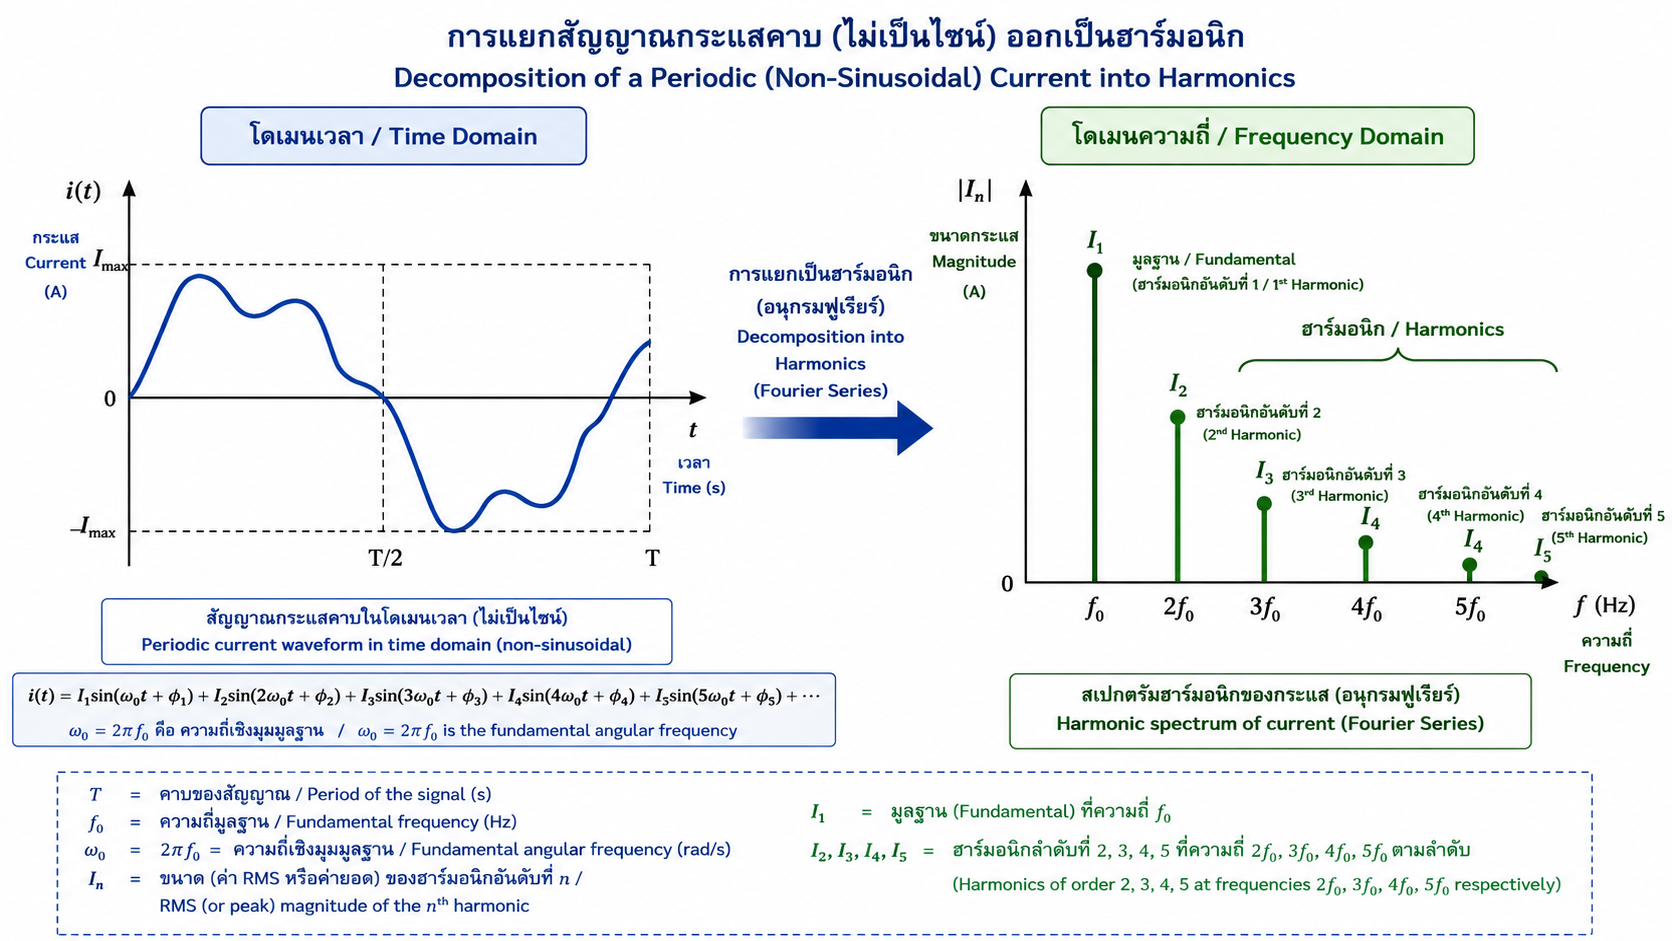
\includegraphics[width=0.8\textwidth]{images/chapter5/figure-01.png}
    \caption{ความเชื่อมโยงระหว่างรูปคลื่นในโดเมนเวลาและสเปกตรัมความถี่}
\end{figure}



\subsection{7.2 รูปคลื่นไซน์ รูปคลื่นสี่เหลี่ยม รูปคลื่นสามเหลี่ยม และรูปคลื่นฟันเลื่อย}

รูปคลื่นมาตรฐานทั้งสี่ชนิดมีประโยชน์อย่างมากในการเรียนรู้ เพราะแสดงให้เห็นโดยตรงว่า “ความคม” และ “ความไม่ต่อเนื่อง” ของรูปคลื่นสัมพันธ์กับการลดลงของแอมพลิจูดฮาร์มอนิกอย่างไร

\subsubsection{7.2.1 รูปคลื่นไซน์}

รูปคลื่นไซน์บริสุทธิ์เขียนได้เป็น

\[
x(t)=X_m\sin(\omega_0 t+\phi)
\]

โดย $X_m$ คือค่าสูงสุดหรือ peak value และ $\phi$ คือมุมเฟส หากเป็นไซน์บริสุทธิ์ที่ไม่มี DC สเปกตรัมจะมีเพียงองค์ประกอบที่ความถี่มูลฐานเท่านั้น

ค่าประสิทธิผลของไซน์คือ

\[
X_{\mathrm{rms}}=\frac{X_m}{\sqrt{2}}
\]

\subsubsection{7.2.2 รูปคลื่นสี่เหลี่ยมสมมาตร}

พิจารณารูปคลื่นสี่เหลี่ยมสมมาตรที่มีค่า $+X_m$ และ $-X_m$ อย่างละครึ่งคาบ และมีค่าเฉลี่ยเป็นศูนย์ เนื่องจากเป็นฟังก์ชันคี่ จึงเหลือเฉพาะพจน์ไซน์

\[
x(t)=\frac{4X_m}{\pi}\left(\sin\omega_0 t+\frac{1}{3}\sin3\omega_0 t+\frac{1}{5}\sin5\omega_0 t+\cdots\right)
\]

\textbf{คุณลักษณะสำคัญ}

\begin{itemize}
    \item มีเฉพาะฮาร์มอนิกลำดับคี่ $1,3,5,\ldots$
    \item แอมพลิจูด peak ของฮาร์มอนิกลำดับ $n$ ลดลงประมาณ $1/n$
    \item การลดลงแบบ $1/n$ ค่อนข้างช้า จึงมีฮาร์มอนิกลำดับสูงที่มีนัยสำคัญ
    \item เนื่องจากมีจุดไม่ต่อเนื่อง การประมาณด้วยจำนวนพจน์จำกัดจะเกิด Gibbs phenomenon ใกล้จุดกระโดด
\end{itemize}

\subsubsection{7.2.3 รูปคลื่นสามเหลี่ยมสมมาตร}

รูปคลื่นสามเหลี่ยมสมมาตรที่มีค่า peak $\pm X_m$ สามารถเขียนในรูปอนุกรมไซน์แบบหนึ่งได้เป็น

\[
x(t)=\frac{8X_m}{\pi^2}\left(\sin\omega_0 t-\frac{1}{3^2}\sin3\omega_0 t+\frac{1}{5^2}\sin5\omega_0 t-\cdots\right)
\]

\textbf{คุณลักษณะสำคัญ}

\begin{itemize}
    \item มีเฉพาะฮาร์มอนิกลำดับคี่
    \item แอมพลิจูดลดลงประมาณ $1/n^2$
    \item ลดลงเร็วกว่ารูปคลื่นสี่เหลี่ยม จึงมีความเพี้ยนน้อยกว่าเมื่อเทียบที่สเกลเดียวกัน
    \item รูปคลื่นต่อเนื่อง แต่ความชันเปลี่ยนอย่างฉับพลันที่ยอดและจุดต่ำสุด
\end{itemize}

\subsubsection{7.2.4 รูปคลื่นฟันเลื่อยสมมาตรรอบศูนย์}

สำหรับ sawtooth แบบสมมาตรรอบศูนย์ที่เพิ่มเชิงเส้นจาก $-X_m$ ไป $+X_m$ ภายในหนึ่งคาบ อนุกรมฟูเรียร์รูปหนึ่งคือ

\[
x(t)=\frac{2X_m}{\pi}\left(\sin\omega_0 t-\frac{1}{2}\sin2\omega_0 t+\frac{1}{3}\sin3\omega_0 t-\cdots\right)
\]

เครื่องหมายอาจเปลี่ยนตามการเลือกจุดกำเนิดเวลาและทิศทางของ sawtooth แต่สาระสำคัญคือ

\begin{itemize}
    \item มีทั้งฮาร์มอนิกลำดับคู่และคี่
    \item แอมพลิจูดลดลงประมาณ $1/n$
    \item มีจุดกระโดดหนึ่งครั้งต่อคาบ จึงมีพลังงานกระจายไปยังฮาร์มอนิกลำดับสูงมากกว่ารูปคลื่นสามเหลี่ยม
\end{itemize}

\subsubsection{7.2.5 ตารางเปรียบเทียบรูปคลื่นมาตรฐาน}

\begin{table}[htbp]
    \centering
    \small
    \begin{tabularx}{\textwidth}{>{\raggedright\arraybackslash}p{0.16\textwidth} >{\raggedright\arraybackslash}p{0.16\textwidth} >{\raggedright\arraybackslash}X >{\centering\arraybackslash}p{0.16\textwidth} >{\raggedright\arraybackslash}p{0.20\textwidth}}
        \hline
        \textbf{รูปคลื่น} & \textbf{ฮาร์มอนิกเด่น} & \textbf{การลดลงของแอมพลิจูด} & \textbf{$X_{\mathrm{rms}}$ เมื่อ peak = $X_m$} & \textbf{THD เชิงทฤษฎีของรูปคลื่นอุดมคติ*} \\
        \hline
        ไซน์ & มูลฐานเท่านั้น & ไม่มีฮาร์มอนิก & $X_m/\sqrt{2}$ & 0\% \\
        สี่เหลี่ยมสมมาตร & คี่ & $1/n$ & $X_m$ & ประมาณ 48.34\% \\
        สามเหลี่ยมสมมาตร & คี่ & $1/n^2$ & $X_m/\sqrt{3}$ & ประมาณ 12.12\% \\
        ฟันเลื่อยสมมาตร & คู่และคี่ & $1/n$ & $X_m/\sqrt{3}$ & ประมาณ 80.31\% \\
        \hline
    \end{tabularx}
\end{table}

* ค่า THD ในตารางคำนวณจากองค์ประกอบฮาร์มอนิกทั้งหมดของรูปคลื่นอุดมคติ โดยไม่นับ DC และอ้างองค์ประกอบมูลฐานเป็นตัวหาร ไม่ใช่ “เกณฑ์มาตรฐาน” ของระบบไฟฟ้า

% [รูปที่ 2: เปรียบเทียบรูปคลื่นมาตรฐานและการลดลงของฮาร์มอนิก]
% ประเภทภาพ: Graph / Infographic
% ตำแหน่งที่แนะนำ: หลังตารางเปรียบเทียบรูปคลื่นมาตรฐาน
% วัตถุประสงค์การเรียนรู้: แสดงความสัมพันธ์ระหว่างความเรียบของรูปคลื่นกับอัตราการลดลงของฮาร์มอนิก
% คำอธิบายภาพ: แบ่งเป็นสี่แถว แต่ละแถวมีกราฟเวลาและสเปกตรัมของ sine, square, triangle, sawtooth ที่สเกลเดียวกัน
% องค์ประกอบที่ต้องมี: waveform, spectrum, harmonic order, เส้นแนวโน้ม 1/n และ 1/n²
% ข้อความหรือป้ายกำกับ: “Sine”, “Square”, “Triangle”, “Sawtooth”, “odd harmonics”, “all harmonics”, “1/n”, “1/n²”
% ภาษาของป้ายกำกับ: ไทยและอังกฤษ
% สัดส่วนภาพ: 16:9
% Image Generation Prompt: Four-row engineering infographic comparing sine, symmetric square, symmetric triangle, and symmetric sawtooth waveforms. For each row show the time-domain waveform and a discrete harmonic magnitude spectrum. Highlight that square wave has odd harmonics decaying as 1/n, triangle has odd harmonics decaying as 1/n^2, sawtooth has even and odd harmonics decaying as 1/n, and sine has only the fundamental. White background, clean textbook vector graphics, bilingual Thai-English labels, 16:9.
% Graph Generation Prompt: Generate normalized waveforms with peak ±1 over two periods and corresponding normalized Fourier coefficient magnitude spectra up to harmonic order 15. Use consistent axes. Label harmonic order n and normalized magnitude.
% Alt Text: สี่ชุดกราฟเปรียบเทียบ sine, square, triangle และ sawtooth พร้อมสเปกตรัม แสดงว่ารูปสามเหลี่ยมมีฮาร์มอนิกลดลงเร็วที่สุดในกลุ่มรูปคลื่นไม่เป็นไซน์

\begin{figure}[htbp]
    \centering
    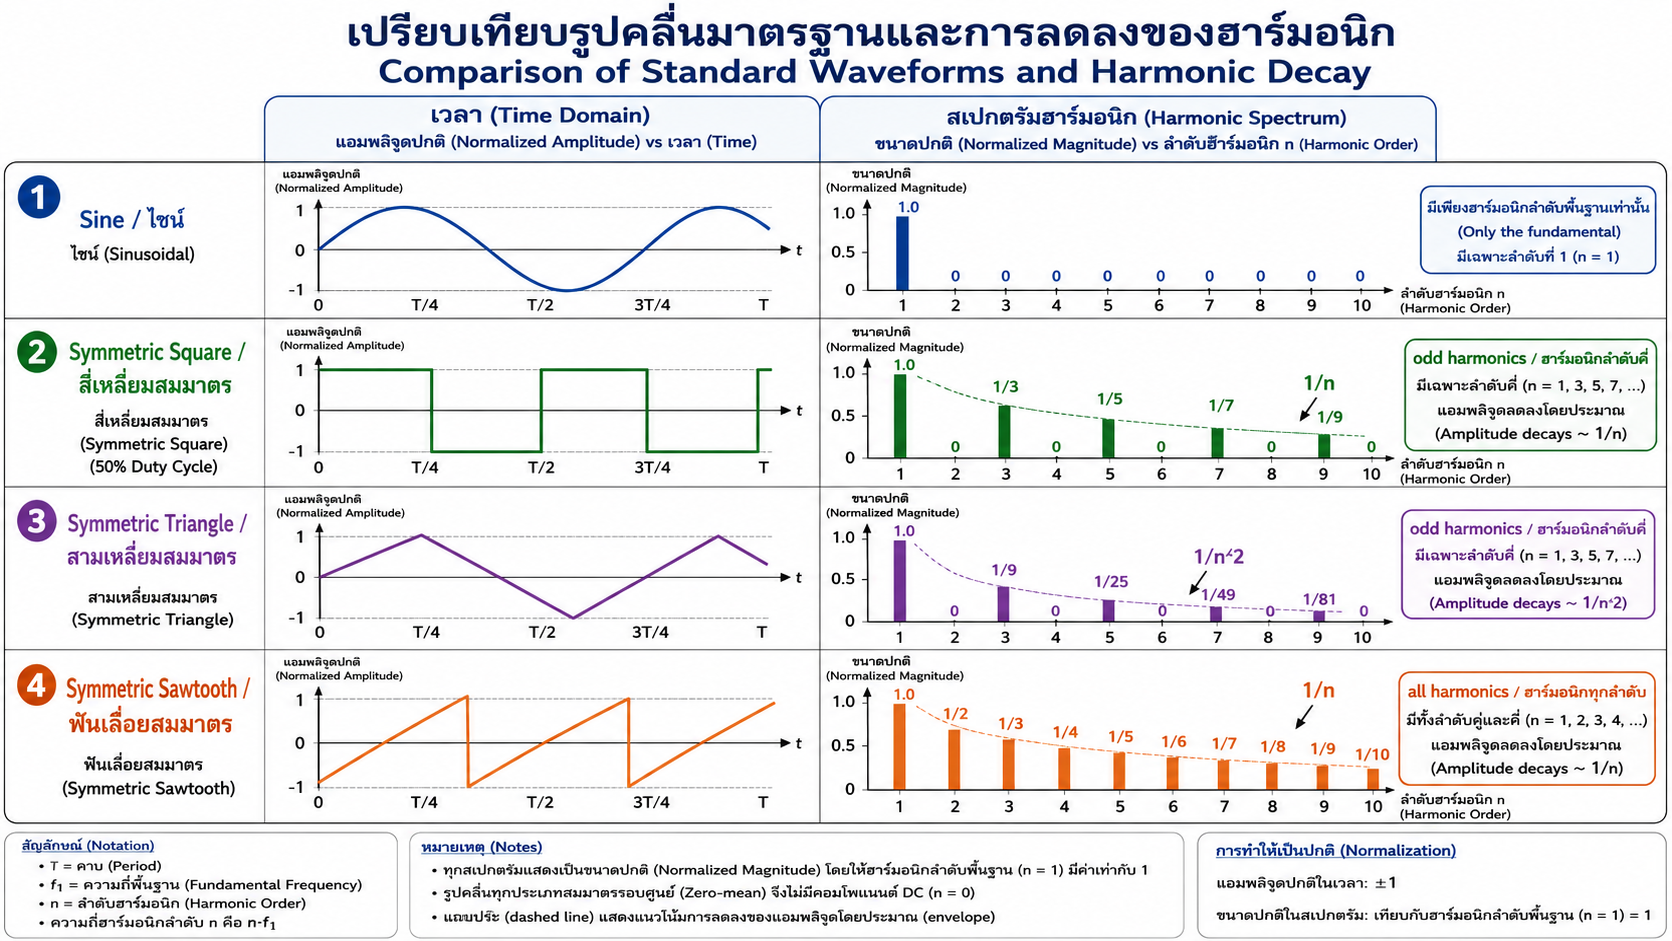
\includegraphics[width=0.8\textwidth]{images/chapter5/figure-02.png}
    \caption{เปรียบเทียบรูปคลื่นมาตรฐานและการลดลงของฮาร์มอนิก}
\end{figure}



\subsection{7.3 การวิเคราะห์ฮาร์มอนิกของรูปคลื่นไฟฟ้า}

\subsubsection{7.3.1 รูปทั่วไปของอนุกรมฟูเรียร์}

สำหรับสัญญาณเป็นคาบ $x(t)$ คาบ $T$ รูปตรีโกณมิติทั่วไปคือ

\[
x(t)=\frac{a_0}{2}+\sum_{n=1}^{\infty}\left[a_n\cos(n\omega_0 t)+b_n\sin(n\omega_0 t)\right]
\]

โดย

\[
a_0=\frac{2}{T}\int_{t_0}^{t_0+T}x(t)\,dt
\]

\[
a_n=\frac{2}{T}\int_{t_0}^{t_0+T}x(t)\cos(n\omega_0 t)\,dt
\]

\[
b_n=\frac{2}{T}\int_{t_0}^{t_0+T}x(t)\sin(n\omega_0 t)\,dt
\]

\textbf{ที่มา:} สมการเกิดจากสมบัติออร์โทโกนัลของไซน์และโคไซน์บนช่วงหนึ่งคาบ ทำให้สามารถแยกค่าสัมประสิทธิ์ของแต่ละความถี่ออกจากกันได้

\textbf{ความหมายของตัวแปร}

\begin{itemize}
    \item $a_0/2$ คือ DC component หรือค่าเฉลี่ย
    \item $a_n$ คือสัมประสิทธิ์โคไซน์ของฮาร์มอนิกลำดับที่ $n$
    \item $b_n$ คือสัมประสิทธิ์ไซน์ของฮาร์มอนิกลำดับที่ $n$
    \item $n\omega_0$ คือความถี่เชิงมุมของฮาร์มอนิกลำดับที่ $n$
\end{itemize}

\textbf{เงื่อนไขการใช้:} เหมาะกับสัญญาณเป็นคาบที่มีคุณสมบัติทางคณิตศาสตร์เพียงพอสำหรับการขยายเป็นอนุกรมฟูเรียร์ เช่น มีจำนวนจุดไม่ต่อเนื่องจำกัดในหนึ่งคาบและอินทิเกรตได้เป็นช่วง ๆ

\subsubsection{7.3.2 รูปแอมพลิจูด–เฟส}

พจน์ของฮาร์มอนิกลำดับที่ $n$ สามารถเขียนเป็น

\[
\begin{aligned}
    a_n\cos(n\omega_0 t)+b_n\sin(n\omega_0 t) \\
    =A_n\cos(n\omega_0 t-\theta_n)
\end{aligned}
\]

เมื่อ

\[
A_n=\sqrt{a_n^2+b_n^2}
\]

และ

\[
\theta_n=\operatorname{atan2}(b_n,a_n)
\]

การใช้ $\operatorname{atan2}$ ช่วยระบุควอดแรนต์ของมุมได้ถูกต้องกว่าการใช้ $\tan^{-1}(b_n/a_n)$ เพียงอย่างเดียว

\textbf{ความหมายทางกายภาพ:} $A_n$ บอก “ขนาด” ขององค์ประกอบความถี่ ส่วน $\theta_n$ บอกตำแหน่งเฟสขององค์ประกอบนั้นเมื่อเทียบกับแกนอ้างอิงเวลา

\subsubsection{7.3.3 สเปกตรัมขนาดแบบ peak และ RMS}

ในวิชาคณิตศาสตร์ ฟูเรียร์มักใช้ $A_n$ เป็น peak amplitude แต่ในวิศวกรรมกำลังมักรายงานขนาดฮาร์มอนิกเป็น RMS ดังนั้นต้องระบุชนิดของขนาดให้ชัดเจน

สำหรับองค์ประกอบไซน์หรือโคไซน์หนึ่งความถี่

\[
X_{n,\mathrm{rms}}=\frac{A_n}{\sqrt{2}}
\]

จึงควรหลีกเลี่ยงการนำ peak amplitude ไปใช้ในสูตร THD ที่กำหนดด้วย RMS โดยไม่แปลงหน่วยก่อน ถึงแม้อัตราส่วนบางกรณีจะให้ค่าเท่ากันหากทุกพจน์ใช้ชนิดเดียวกัน แต่การกำหนดมาตรฐานการคำนวณให้ชัดเจนช่วยลดความผิดพลาด

\subsubsection{7.3.4 Harmonic order กับความถี่จริง}

ถ้าระบบมี $f_0=50$ Hz

\begin{table}[htbp]
    \centering
    \begin{tabular}{r r}
        \hline
        \textbf{Harmonic order} & \textbf{ความถี่} \\
        \hline
        1 & 50 Hz \\
        2 & 100 Hz \\
        3 & 150 Hz \\
        5 & 250 Hz \\
        7 & 350 Hz \\
        11 & 550 Hz \\
        13 & 650 Hz \\
        \hline
    \end{tabular}
\end{table}

ในระบบ 60 Hz ให้คูณลำดับฮาร์มอนิกด้วย 60 แทน การระบุ “ลำดับฮาร์มอนิก” จึงสะดวกต่อการเปรียบเทียบระบบที่มีความถี่มูลฐานต่างกัน

\subsubsection{ตัวอย่างที่ 1: อ่านองค์ประกอบฮาร์มอนิกจากสมการรูปคลื่น}

\textbf{ตัวอย่างเพิ่มเติมเพื่อการเรียนรู้}

กำหนดกระแส

\[
i(t)=10\sqrt{2}\sin(2\pi 50t)+3\sqrt{2}\sin(2\pi 150t-20^\circ)+1.5\sqrt{2}\sin(2\pi 250t+30^\circ)\ \text{A}
\]

จงระบุความถี่มูลฐาน ลำดับฮาร์มอนิก ขนาด RMS และเฟสของแต่ละองค์ประกอบ

\textbf{ขั้นที่ 1 วิเคราะห์โจทย์} \\
รูปคลื่นประกอบด้วยไซน์สามความถี่ 50, 150 และ 250 Hz

\textbf{ขั้นที่ 2 กำหนดความถี่มูลฐาน}

\[
f_0=50\ \text{Hz}
\]

\textbf{ขั้นที่ 3 หา harmonic order}

\[
150/50=3,\qquad 250/50=5
\]

ดังนั้นมี fundamental, 3rd และ 5th harmonic

\textbf{ขั้นที่ 4 แปลง peak เป็น RMS} \\
เนื่องจาก coefficient ของไซน์เขียนเป็น $\sqrt{2}I_{\mathrm{rms}}$

\begin{itemize}
    \item $I_1=10$ A RMS, phase $0^\circ$
    \item $I_3=3$ A RMS, phase $-20^\circ$
    \item $I_5=1.5$ A RMS, phase $+30^\circ$
\end{itemize}

\textbf{ขั้นที่ 5 ตรวจสอบความสมเหตุสมผล} \\
ฮาร์มอนิกมีขนาดเล็กกว่ามูลฐาน จึงสอดคล้องกับรูปคลื่นที่ยังมีลักษณะพื้นฐาน 50 Hz แต่เกิดการเพี้ยน

\textbf{คำตอบ}

\begin{table}[htbp]
    \centering
    \begin{tabular}{l r r r}
        \hline
        \textbf{องค์ประกอบ} & \textbf{ความถี่} & \textbf{RMS} & \textbf{เฟส} \\
        \hline
        Fundamental & 50 Hz & 10 A & $0^\circ$ \\
        3rd harmonic & 150 Hz & 3 A & $-20^\circ$ \\
        5th harmonic & 250 Hz & 1.5 A & $+30^\circ$ \\
        \hline
    \end{tabular}
\end{table}

% [รูปที่ 3: การสังเคราะห์รูปคลื่นจาก fundamental, 3rd และ 5th harmonic]
% ประเภทภาพ: Graph
% ตำแหน่งที่แนะนำ: หลังตัวอย่างที่ 1
% วัตถุประสงค์การเรียนรู้: แสดงว่าการบวกฮาร์มอนิกเปลี่ยนรูปร่างของสัญญาณอย่างไร
% คำอธิบายภาพ: กราฟบนแสดงองค์ประกอบ 50, 150, 250 Hz แยกเส้น กราฟล่างแสดงผลรวม
% องค์ประกอบที่ต้องมี: แกนเวลา ms, กระแส A, legend ของ fundamental/3rd/5th/sum
% ข้อความหรือป้ายกำกับ: “Fundamental 50 Hz”, “3rd 150 Hz”, “5th 250 Hz”, “Resultant waveform”
% ภาษาของป้ายกำกับ: ไทยและอังกฤษ
% สัดส่วนภาพ: 16:9
% Image Generation Prompt: Engineering mathematics graph showing three sinusoidal current components at 50 Hz, 150 Hz, and 250 Hz and their summed distorted waveform. Use two panels: individual harmonics on top and resultant waveform below. Precise axes in milliseconds and amperes, bilingual Thai-English labels, white background, textbook vector style, 16:9.
% Graph Generation Prompt: Plot i1(t)=10√2 sin(2π50t), i3(t)=3√2 sin(2π150t−20°), i5(t)=1.5√2 sin(2π250t+30°), and i(t)=i1+i3+i5 from 0 to 40 ms. Use amperes and milliseconds.
% Alt Text: กราฟแสดงไซน์สามความถี่และผลรวมที่เกิดเป็นกระแสผิดรูปจากฮาร์มอนิกอันดับ 3 และ 5

\begin{figure}[htbp]
    \centering
    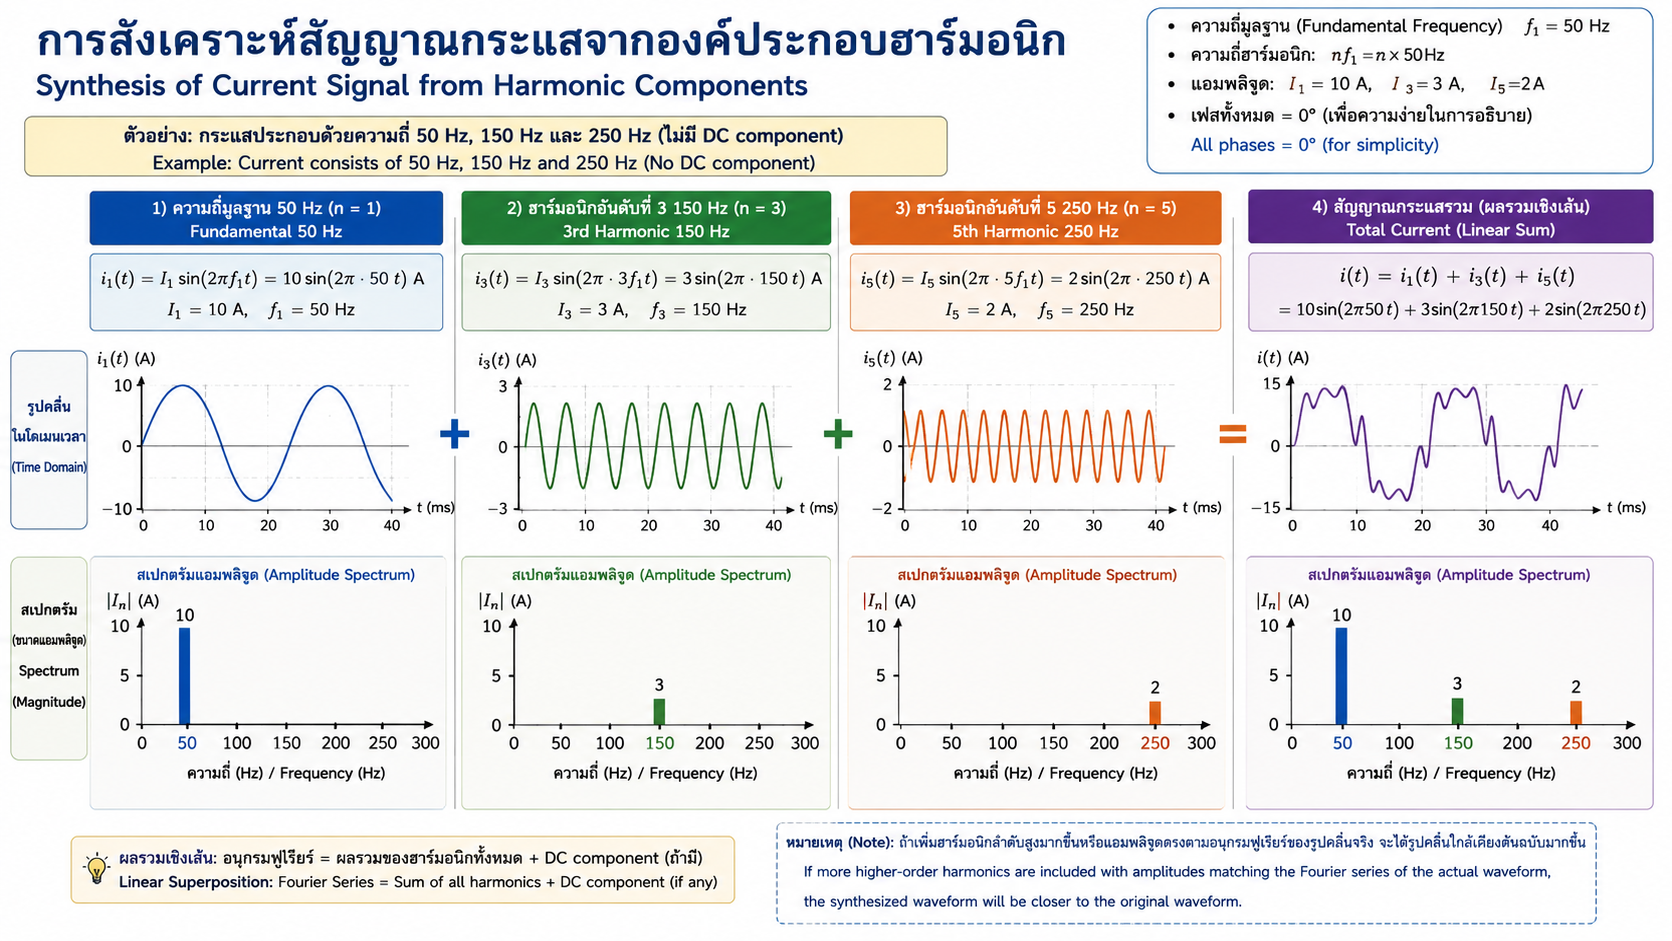
\includegraphics[width=0.8\textwidth]{images/chapter5/figure-03.png}
    \caption{การสังเคราะห์รูปคลื่นจาก fundamental, 3rd และ 5th harmonic}
\end{figure}



\subsection{7.4 ความสัมพันธ์ระหว่างอนุกรมฟูเรียร์กับคุณภาพกำลังไฟฟ้า}

\subsubsection{7.4.1 จากโหลดไม่เชิงเส้นสู่แรงดันเพี้ยน}

พิจารณาระบบจ่ายไฟอย่างง่ายที่มีแรงดันต้นทางเชิงอุดมคติ $v_s(t)$ และอิมพีแดนซ์ระบบ $Z_s$ หากโหลดไม่เชิงเส้นดึงกระแส

\[
i(t)=\sum_{n=1}^{\infty} i_n(t)
\]

กระแสแต่ละฮาร์มอนิกจะสร้างแรงดันตกคร่อมที่ความถี่เดียวกันผ่านอิมพีแดนซ์ของระบบ ดังนั้นแรงดันที่จุดโหลดสามารถมองเชิงแนวคิดได้ว่า

\[
V_n \approx I_n Z_s(n\omega_0)
\]

สมการนี้ไม่ใช่แบบจำลองระบบกำลังเต็มรูปแบบ แต่ช่วยอธิบายหลักสำคัญว่า \textbf{ฮาร์มอนิกกระแสทำให้เกิดฮาร์มอนิกแรงดันได้เมื่อระบบมีอิมพีแดนซ์ไม่เป็นศูนย์}

\subsubsection{7.4.2 PCC และมุมมองของมาตรฐาน}

IEEE 519-2022 กำหนดเป้าหมายสำหรับการออกแบบระบบที่มีทั้งโหลดเชิงเส้นและไม่เชิงเส้น และประเมินขีดจำกัดความเพี้ยนของแรงดันและกระแสแบบ steady-state ที่ \textbf{Point of Common Coupling (PCC)} แนวคิดนี้มีความสำคัญต่อผู้เรียน เพราะทำให้ไม่สับสนระหว่าง

\begin{enumerate}
    \item รูปคลื่นภายในอุปกรณ์หนึ่งชิ้น
    \item กระแสที่อุปกรณ์ฉีดเข้าสู่ระบบ
    \item ผลรวมของโหลดหลายชนิดที่ PCC
    \item ความเพี้ยนของแรงดันระบบที่ผู้ใช้อื่นร่วมกันได้รับ
\end{enumerate}

ดังนั้นค่า THD ที่วัดจากอุปกรณ์เดี่ยวในห้องทดลองไม่ควรถูกนำไปสรุปว่า “ผ่านหรือไม่ผ่าน IEEE 519” โดยตรง หากยังไม่ได้กำหนดตำแหน่งวัด เงื่อนไขระบบ และตัวชี้วัดที่มาตรฐานกำหนด

\subsubsection{7.4.3 ฮาร์มอนิกกับ power quality ไม่ใช่เรื่องเดียวกันทั้งหมด}

คุณภาพกำลังไฟฟ้ายังครอบคลุมความถี่ แรงดันตก/เกินชั่วขณะ flicker interruption unbalance transient และปรากฏการณ์อื่น การวิเคราะห์ฮาร์มอนิกจึงเป็นเพียงส่วนหนึ่งของ power quality แต่เป็นส่วนที่เหมาะกับการใช้ Fourier analysis อย่างเด่นชัด

% [รูปที่ 4: เส้นทางการเกิดฮาร์มอนิกในระบบไฟฟ้า]
% ประเภทภาพ: Block Diagram / Technical Illustration
% ตำแหน่งที่แนะนำ: หัวข้อ 7.4
% วัตถุประสงค์การเรียนรู้: แสดงเหตุ–ผลจากโหลดไม่เชิงเส้นไปยังความเพี้ยนที่ PCC
% คำอธิบายภาพ: แหล่งจ่ายไซน์ → อิมพีแดนซ์ระบบ → PCC → โหลดไม่เชิงเส้น โดยมีลูกศร current harmonics ไหลจากโหลด และ voltage distortion เกิดที่ PCC
% องค์ประกอบที่ต้องมี: AC source, source impedance, PCC, nonlinear load, harmonic current arrows, distorted PCC voltage
% ข้อความหรือป้ายกำกับ: “Source”, “System impedance”, “PCC”, “Nonlinear load”, “Harmonic current”, “Voltage distortion”
% ภาษาของป้ายกำกับ: ไทยและอังกฤษ
% สัดส่วนภาพ: 16:9
% Image Generation Prompt: Clean electrical engineering block diagram illustrating harmonic propagation in a power system. Show an ideal sinusoidal AC source, source/system impedance, a labeled Point of Common Coupling (PCC), and a nonlinear load such as a rectifier or switching power supply. Show distorted harmonic current flowing from the load through the system impedance and resulting voltage distortion at the PCC. Bilingual Thai-English labels, white background, vector textbook style, 16:9.
% Alt Text: แผนภาพแสดงโหลดไม่เชิงเส้นสร้างกระแสฮาร์มอนิกซึ่งไหลผ่านอิมพีแดนซ์ระบบและทำให้แรงดันที่ PCC เพี้ยน

\begin{figure}[htbp]
    \centering
    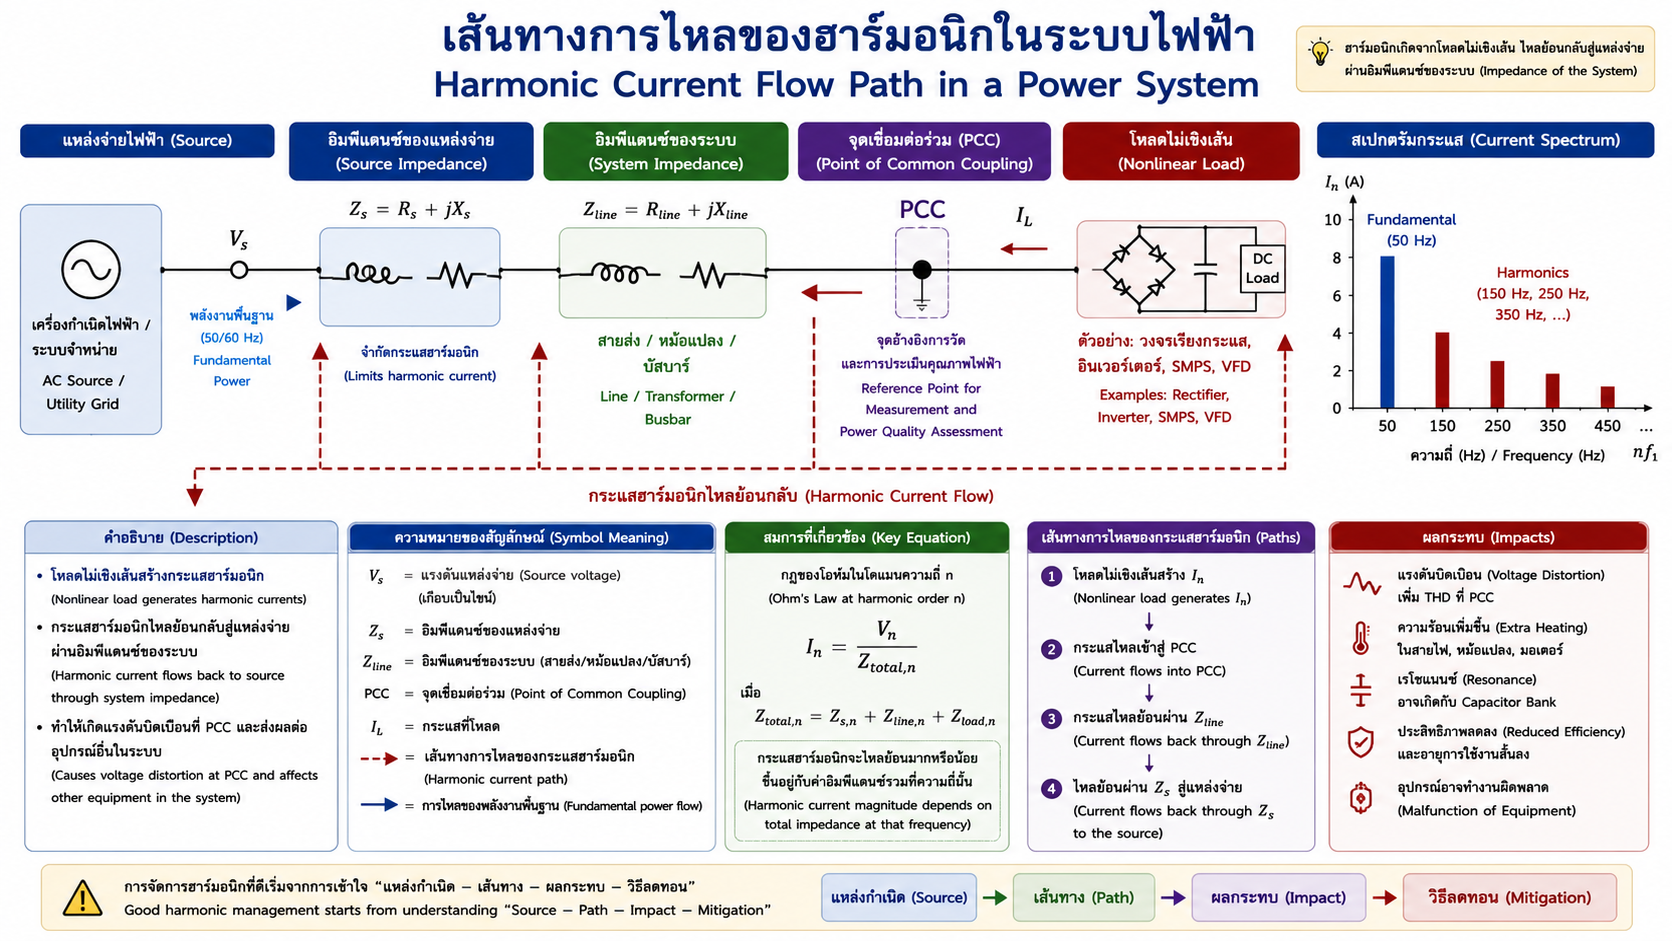
\includegraphics[width=0.8\textwidth]{images/chapter5/figure-04.png}
    \caption{เส้นทางการเกิดฮาร์มอนิกในระบบไฟฟ้า}
\end{figure}


\subsection{7.5 ค่าประสิทธิผลของสัญญาณไฟฟ้า}

\subsubsection{7.5.1 ความหมายของ RMS}

ค่าประสิทธิผล หรือ \textbf{Root Mean Square (RMS)} ของสัญญาณเป็นคาบ $x(t)$ นิยามโดย

\[
X_{\mathrm{rms}}=\sqrt{\frac{1}{T}\int_{t_0}^{t_0+T}x^2(t)\,dt}
\]

สมการนี้มีขั้นตอนตามชื่อโดยตรง

\begin{enumerate}
    \item \textbf{Square:} ยกกำลังสองสัญญาณ เพื่อทำให้ค่าบวกและลบไม่หักล้างกัน
    \item \textbf{Mean:} หาเฉลี่ยตลอดหนึ่งคาบ
    \item \textbf{Root:} ถอดรากที่สองเพื่อให้หน่วยกลับมาเหมือนปริมาณเดิม
\end{enumerate}

หาก $x(t)$ เป็นแรงดัน หน่วยของ $X_{\mathrm{rms}}$ คือโวลต์ หากเป็นกระแส หน่วยคือแอมแปร์

\subsubsection{7.5.2 ความหมายทางกายภาพ}

สำหรับแรงดันหรือกระแสที่จ่ายให้ตัวต้านทาน RMS คือค่ากระแสตรงที่ก่อให้เกิดกำลังเฉลี่ยหรือผลความร้อนเท่ากัน ตัวอย่างเช่น ถ้ากระแส AC มี $I_{\mathrm{rms}}=5$ A ไหลผ่านตัวต้านทาน $R$ กำลังเฉลี่ยที่ตัวต้านทานรับคือ

\[
P=I_{\mathrm{rms}}^2R
\]

แม้ว่ารูปคลื่นกระแสจะไม่เป็นไซน์ก็ตาม ตราบใดที่ $R$ เป็นตัวต้านทานเชิงอุดมคติและใช้ค่า true RMS ของกระแสนั้น

\subsubsection{7.5.3 RMS จากองค์ประกอบฟูเรียร์: Parseval relation}

ถ้าสัญญาณเขียนได้เป็น

\[
x(t)=X_{\mathrm{DC}}+\sum_{n=1}^{\infty}x_n(t)
\]

โดย $x_n(t)$ เป็นไซน์/โคไซน์ของฮาร์มอนิกลำดับที่ $n$ และองค์ประกอบแต่ละความถี่ตั้งฉากกันในความหมายของอินทิกรัลตลอดหนึ่งคาบ จะได้

\[
X_{\mathrm{rms}}^2=X_{\mathrm{DC}}^2+\sum_{n=1}^{\infty}X_{n,\mathrm{rms}}^2
\]

หรือ

\[
X_{\mathrm{rms}}=\sqrt{X_{\mathrm{DC}}^2+X_{1,\mathrm{rms}}^2+X_{2,\mathrm{rms}}^2+\cdots}
\]

\textbf{ความหมายสำคัญ:} RMS รวมไม่ได้เท่ากับผลบวกธรรมดาของ RMS แต่เป็น \textbf{รากที่สองของผลบวกกำลังสอง} ขององค์ประกอบที่ออร์โทโกนัลกัน

หากใช้สัมประสิทธิ์ตรีโกณมิติแบบ peak

\[
x(t)=\frac{a_0}{2}+\sum_{n=1}^{\infty}[a_n\cos(n\omega_0t)+b_n\sin(n\omega_0t)]
\]

จะได้

\[
X_{\mathrm{rms}}^2=\left(\frac{a_0}{2}\right)^2+\frac{1}{2}\sum_{n=1}^{\infty}(a_n^2+b_n^2)
\]

\textbf{สมมติฐานและข้อจำกัด:} สมการนี้ใช้กับสัญญาณเป็นคาบที่มี Fourier series และค่ากำลังเฉลี่ยจำกัด หากเป็นสัญญาณ transient หรือไม่เป็นคาบ ควรใช้กรอบ Fourier transform หรือวิธีวิเคราะห์สัญญาณอื่น

\subsubsection{ตัวอย่างที่ 2: คำนวณ RMS จากฮาร์มอนิก}

\textbf{ตัวอย่างเพิ่มเติมเพื่อการเรียนรู้}

กระแสหนึ่งมีองค์ประกอบ RMS ดังนี้

\begin{itemize}
    \item fundamental: $I_1=10$ A
    \item 3rd harmonic: $I_3=3$ A
    \item 5th harmonic: $I_5=1.5$ A
    \item 7th harmonic: $I_7=1$ A
\end{itemize}

ไม่มี DC component จงหา $I_{\mathrm{rms}}$

\textbf{ขั้นที่ 1 วิเคราะห์ระบบ} \\
ฮาร์มอนิกแต่ละลำดับเป็นความถี่ต่างกัน จึงรวมแบบ root-sum-square

\textbf{ขั้นที่ 2 เลือกสมการ}

\[
I_{\mathrm{rms}}=\sqrt{I_1^2+I_3^2+I_5^2+I_7^2}
\]

\textbf{ขั้นที่ 3 แทนค่า}

\[
I_{\mathrm{rms}}=\sqrt{10^2+3^2+1.5^2+1^2}
\]

\[
=\sqrt{100+9+2.25+1}
\]

\[
=\sqrt{112.25}=10.59\ \text{A}
\]

\textbf{ขั้นที่ 4 ตรวจสอบหน่วยและความสมเหตุสมผล} \\
ค่า RMS รวมต้องมากกว่า 10 A เพราะมีฮาร์มอนิกเพิ่มเข้ามา แต่ไม่ควรเป็น $10+3+1.5+1=15.5$ A เพราะองค์ประกอบไม่อยู่เฟสและความถี่เดียวกันตลอดเวลา

\textbf{คำตอบ:}

\[
\boxed{I_{\mathrm{rms}}\approx10.59\ \text{A}}
\]

\subsubsection{7.5.4 RMS ของรูปคลื่นมาตรฐาน}

\begin{itemize}
    \item ไซน์ peak $X_m$:
\end{itemize}

\[
X_{\mathrm{rms}}=\frac{X_m}{\sqrt{2}}
\]

\begin{itemize}
    \item สี่เหลี่ยมสมมาตร $\pm X_m$:
\end{itemize}

\[
X_{\mathrm{rms}}=X_m
\]

\begin{itemize}
    \item สามเหลี่ยมสมมาตร $\pm X_m$:
\end{itemize}

\[
X_{\mathrm{rms}}=\frac{X_m}{\sqrt{3}}
\]

\begin{itemize}
    \item sawtooth สมมาตร $\pm X_m$:
\end{itemize}

\[
X_{\mathrm{rms}}=\frac{X_m}{\sqrt{3}}
\]

\subsubsection{7.5.5 ค่าเฉลี่ยไม่ใช่ RMS}

รูปคลื่นสี่เหลี่ยมสมมาตร $+10$ V และ $-10$ V มีค่าเฉลี่ยเท่ากับศูนย์ แต่ RMS เท่ากับ 10 V ดังนั้นการใช้ค่าเฉลี่ยเพื่อประเมินผลความร้อนของ AC จะผิดพลาดอย่างมาก



\subsection{7.6 กำลังไฟฟ้าเฉลี่ยและกำลังไฟฟ้าในรูปคลื่นไม่เป็นไซน์}

\subsubsection{7.6.1 นิยามกำลังทันทีและกำลังเฉลี่ย}

กำลังไฟฟ้าทันทีคือ

\[
p(t)=v(t)i(t)
\]

กำลังไฟฟ้าเฉลี่ยในหนึ่งคาบคือ

\[
P=\frac{1}{T}\int_{t_0}^{t_0+T}v(t)i(t)\,dt
\]

สมการนี้เป็นนิยามพื้นฐานที่ใช้ได้ทั้งกรณีไซน์และไม่เป็นไซน์

\subsubsection{7.6.2 กำลังเฉลี่ยเมื่อแรงดันและกระแสมีฮาร์มอนิก}

ให้

\[
v(t)=V_{\mathrm{DC}}+\sum_{n=1}^{\infty}v_n(t)
\]

และ

\[
i(t)=I_{\mathrm{DC}}+\sum_{n=1}^{\infty}i_n(t)
\]

ด้วยสมบัติออร์โทโกนัล องค์ประกอบต่างความถี่มีค่าเฉลี่ยของผลคูณเป็นศูนย์เมื่ออินทิเกรตตลอดคาบร่วม ดังนั้นกำลังเฉลี่ยสามารถเขียนได้เป็น

\[
P=V_{\mathrm{DC}}I_{\mathrm{DC}}+\sum_{n=1}^{\infty}V_{n,\mathrm{rms}}I_{n,\mathrm{rms}}\cos\phi_n
\]

เมื่อ $\phi_n$ คือมุมเฟสต่างระหว่างแรงดันและกระแสของฮาร์มอนิกลำดับเดียวกัน

\textbf{ความหมายทางกายภาพ:} 50 Hz ของแรงดันสร้างกำลังเฉลี่ยกับ 50 Hz ของกระแส, 150 Hz ของแรงดันสร้างกำลังเฉลี่ยกับ 150 Hz ของกระแส เป็นต้น ส่วนการคูณข้ามความถี่จะเฉลี่ยเป็นศูนย์ในช่วงคาบที่เหมาะสม

\subsubsection{7.6.3 Apparent power และ true power factor}

โดยทั่วไปกำหนด apparent power เป็น

\[
S=V_{\mathrm{rms}}I_{\mathrm{rms}}
\]

หน่วย volt-ampere (VA) และ true power factor เป็น

\[
\mathrm{PF}=\frac{P}{V_{\mathrm{rms}}I_{\mathrm{rms}}}
\]

สำหรับกรณีไซน์บริสุทธิ์ทั้งแรงดันและกระแส PF ลดรูปเป็น $\cos\phi$ แต่เมื่อรูปคลื่นไม่เป็นไซน์ การใช้เพียง $\cos\phi_1$ อาจไม่แทน true PF

\subsubsection{7.6.4 กรณีแรงดันเป็นไซน์ แต่กระแสเพี้ยน}

ถ้าแรงดันมีเฉพาะ fundamental และไม่มี DC

\[
v(t)=v_1(t)
\]

กำลังเฉลี่ยเกิดจาก fundamental current เท่านั้น

\[
P=V_1I_1\cos\phi_1
\]

แต่

\[
I_{\mathrm{rms}}=\sqrt{I_1^2+I_2^2+I_3^2+\cdots}
\]

ดังนั้น

\[
\mathrm{PF}=\frac{V_1I_1\cos\phi_1}{V_1I_{\mathrm{rms}}}
\]

\[
\mathrm{PF}=\frac{I_1}{I_{\mathrm{rms}}}\cos\phi_1
\]

เทอม

\[
\frac{I_1}{I_{\mathrm{rms}}}
\]

สะท้อนผลของ waveform distortion ขณะที่ $\cos\phi_1$ สะท้อน displacement ระหว่าง fundamental voltage และ fundamental current

\subsubsection{ตัวอย่างที่ 3: ตัวประกอบกำลังเมื่อกระแสมีฮาร์มอนิก}

\textbf{ตัวอย่างเพิ่มเติมเพื่อการเรียนรู้}

แรงดันจ่ายเป็นไซน์บริสุทธิ์ $V_1=230$ V RMS โหลดดึงกระแส

\begin{itemize}
    \item $I_1=8$ A RMS ที่ displacement factor $\cos\phi_1=0.90$
    \item $I_3=2.5$ A RMS
    \item $I_5=1.5$ A RMS
\end{itemize}

จงหากระแส RMS รวม กำลังจริง apparent power และ true PF

\textbf{ขั้นที่ 1 กระแส RMS รวม}

\[
I_{\mathrm{rms}}=\sqrt{8^2+2.5^2+1.5^2}
\]

\[
=\sqrt{64+6.25+2.25}=\sqrt{72.5}=8.51\ \text{A}
\]

\textbf{ขั้นที่ 2 กำลังจริง} \\
เพราะแรงดันมีเฉพาะ 50 Hz จึงมีเฉพาะ $V_1I_1\cos\phi_1$

\[
P=230(8)(0.90)=1656\ \text{W}
\]

\textbf{ขั้นที่ 3 apparent power}

\[
S=230(8.51)=1957.3\ \text{VA}
\]

\textbf{ขั้นที่ 4 true PF}

\[
\mathrm{PF}=\frac{1656}{1957.3}=0.846
\]

\textbf{การแปลความหมาย:} แม้ displacement factor ของ fundamental จะเป็น 0.90 แต่ true PF เหลือประมาณ 0.846 เนื่องจากฮาร์มอนิกเพิ่ม $I_{\mathrm{rms}}$ โดยไม่ได้สร้างกำลังจริงเพิ่มในกรณีที่แรงดันไม่มีฮาร์มอนิกสอดคล้องกัน

\textbf{คำตอบ}

\[
\boxed{I_{\mathrm{rms}}\approx8.51\ \text{A},\quad P=1.656\ \text{kW},\quad S\approx1.957\ \text{kVA},\quad PF\approx0.846}
\]

% [รูปที่ 5: กำลังไฟฟ้าในโดเมนฮาร์มอนิก]
% ประเภทภาพ: Infographic / Spectrum Diagram
% ตำแหน่งที่แนะนำ: หลังหัวข้อ 7.6.2
% วัตถุประสงค์การเรียนรู้: แสดงว่ากำลังเฉลี่ยจับคู่แรงดันและกระแสที่ฮาร์มอนิกลำดับเดียวกัน
% คำอธิบายภาพ: สเปกตรัมแรงดันด้านบนและกระแสด้านล่าง พร้อมลูกศรเชื่อม $V_1$ กับ $I_1$, $V_3$ กับ $I_3$, $V_5$ กับ $I_5$ และแสดงสูตร $P=\sum V_nI_n\cos\phi_n$
% องค์ประกอบที่ต้องมี: harmonic order, RMS magnitude, phase labels, matching arrows
% ข้อความหรือป้ายกำกับ: “Same-order harmonic power contribution”, “ต่างความถี่เฉลี่ยเป็นศูนย์”
% ภาษาของป้ายกำกับ: ไทยและอังกฤษ
% สัดส่วนภาพ: 16:9
% Image Generation Prompt: Engineering infographic illustrating average power in nonsinusoidal voltage and current. Show separate voltage and current harmonic spectra with matching arrows between V1-I1, V3-I3, V5-I5 and annotate P = sum(Vn_rms In_rms cos(phi_n)). Emphasize that cross-frequency products average to zero over a common period. White background, bilingual Thai-English labels, clean textbook vector style, 16:9.
% Alt Text: สเปกตรัมแรงดันและกระแสแสดงการจับคู่ฮาร์มอนิกลำดับเดียวกันในการคำนวณกำลังเฉลี่ย

\begin{figure}[htbp]
    \centering
    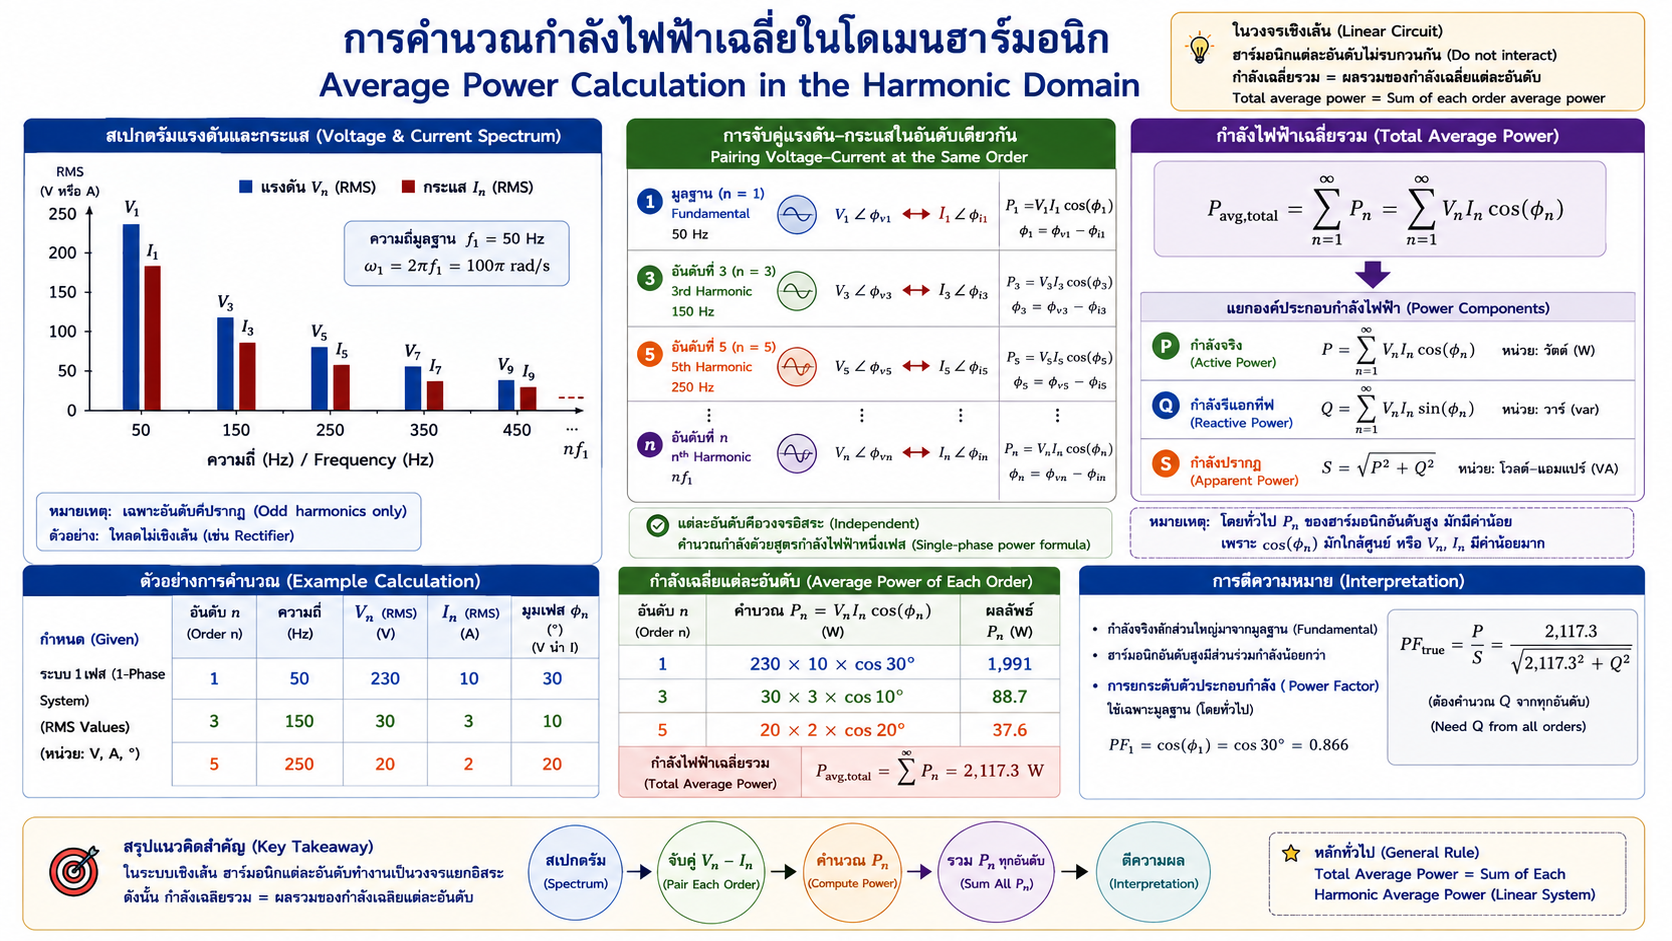
\includegraphics[width=0.8\textwidth]{images/chapter5/figure-05.png}
    \caption{กำลังไฟฟ้าในโดเมนฮาร์มอนิก}
\end{figure}



\subsection{7.7 การวิเคราะห์ Total Harmonic Distortion หรือ THD}

\subsubsection{7.7.1 นิยาม THD}

สำหรับแรงดันที่มี fundamental RMS เท่ากับ $V_1$ และฮาร์มอนิกตั้งแต่ลำดับที่ 2 ขึ้นไป

\[
\mathrm{THD}_V=\frac{\sqrt{V_2^2+V_3^2+V_4^2+\cdots}}{V_1}\times100\%
\]

สำหรับกระแส

\[
\mathrm{THD}_I=\frac{\sqrt{I_2^2+I_3^2+I_4^2+\cdots}}{I_1}\times100\%
\]

โดยทุก $V_n$ และ $I_n$ ต้องใช้ชนิดขนาดเดียวกัน โดยทั่วไปใช้ RMS

\subsubsection{7.7.2 ความสัมพันธ์ระหว่าง THD กับ RMS รวม}

หากไม่มี DC

\[
V_{\mathrm{rms}}^2=V_1^2+\sum_{n=2}^{\infty}V_n^2
\]

ดังนั้น

\[
V_{\mathrm{rms}}=V_1\sqrt{1+\mathrm{THD}_V^2}
\]

เมื่อ THD ในสมการนี้เขียนเป็นอัตราส่วน เช่น 0.05 ไม่ใช่ 5

ในทำนองเดียวกัน

\[
I_{\mathrm{rms}}=I_1\sqrt{1+\mathrm{THD}_I^2}
\]

\subsubsection{7.7.3 THD บอกอะไร และไม่บอกอะไร}

THD มีข้อดีคือสรุปความเพี้ยนเป็นตัวเลขเดียว แต่ไม่ได้บอกว่า

\begin{itemize}
    \item ฮาร์มอนิกลำดับใดเป็นตัวหลัก
    \item เฟสของฮาร์มอนิกเป็นอย่างไร
    \item มี interharmonic หรือไม่
    \item รูปคลื่นเกิด transient หรือไม่
    \item ตำแหน่งวัดอยู่ที่ใด
    \item ค่าเดียวกันเกิดจากสเปกตรัมที่แตกต่างกันมากเพียงใด
\end{itemize}

ดังนั้นในการวิเคราะห์ทางวิศวกรรมควรดู \textbf{ทั้งค่า THD และสเปกตรัมฮาร์มอนิก}

\subsubsection{7.7.4 THD กับ TDD ไม่ใช่สิ่งเดียวกัน}

ในการประเมินกระแสของระบบกำลังตามแนวทาง IEEE 519 มีการใช้ \textbf{Total Demand Distortion (TDD)} ซึ่งอ้างอิงกับ demand current ที่กำหนดตามมาตรฐาน ไม่ใช่ fundamental current ณ ขณะวัดเหมือน THD$_I$ การสอนระดับพื้นฐานจึงควรเน้นให้ผู้เรียนแยกคำสองคำนี้ออกจากกัน และไม่ใช้ THD$_I$ แทน TDD โดยอัตโนมัติ

\subsubsection{ตัวอย่างที่ 4: คำนวณ THD จากสเปกตรัมกระแส}

\textbf{ตัวอย่างเพิ่มเติมเพื่อการเรียนรู้}

จากตัวอย่างก่อนหน้า

\begin{itemize}
    \item $I_1=10$ A
    \item $I_3=3$ A
    \item $I_5=1.5$ A
    \item $I_7=1$ A
\end{itemize}

จงหา $\mathrm{THD}_I$

\textbf{ขั้นที่ 1 เลือกสมการ}

\[
\mathrm{THD}_I=\frac{\sqrt{I_3^2+I_5^2+I_7^2}}{I_1}\times100\%
\]

\textbf{ขั้นที่ 2 แทนค่า}

\[
\mathrm{THD}_I=\frac{\sqrt{3^2+1.5^2+1^2}}{10}\times100\%
\]

\[
=\frac{\sqrt{9+2.25+1}}{10}\times100\%
\]

\[
=\frac{3.5}{10}\times100\%=35\%
\]

\textbf{ขั้นที่ 3 ตรวจสอบด้วย RMS รวม}

\[
I_{\mathrm{rms}}=I_1\sqrt{1+0.35^2}
\]

\[
=10\sqrt{1.1225}=10.59\ \text{A}
\]

ตรงกับผลในตัวอย่างที่ 2

\textbf{คำตอบ:}

\[
\boxed{\mathrm{THD}_I=35\%}
\]

\subsubsection{7.7.5 THD ของรูปคลื่นสี่เหลี่ยมอุดมคติ}

รูปคลื่นสี่เหลี่ยมสมมาตร $\pm X_m$ มี RMS รวมเท่ากับ $X_m$ และ fundamental peak เท่ากับ $4X_m/\pi$ ดังนั้น fundamental RMS คือ

\[
X_1=\frac{4X_m}{\pi\sqrt{2}}
\]

จาก

\[
\mathrm{THD}=\frac{\sqrt{X_{\mathrm{rms}}^2-X_1^2}}{X_1}
\]

ได้

\[
\mathrm{THD}=\sqrt{\frac{\pi^2}{8}-1}
\]

\[
\mathrm{THD}\approx0.4834=48.34\%
\]

ค่าดังกล่าวช่วยให้เห็นว่ารูปคลื่นสี่เหลี่ยมที่ “ดูเป็นรูปทรงเรียบง่าย” ในโดเมนเวลา แท้จริงมีฮาร์มอนิกจำนวนมาก

% [รูปที่ 6: การคำนวณ THD จากสเปกตรัม]
% ประเภทภาพ: Infographic / Graph
% ตำแหน่งที่แนะนำ: หลังตัวอย่างที่ 4
% วัตถุประสงค์การเรียนรู้: ทำให้สูตร THD เชื่อมโยงกับแท่งสเปกตรัมอย่างเป็นรูปธรรม
% คำอธิบายภาพ: แสดงแท่ง fundamental, 3rd, 5th, 7th พร้อม bracket รวมฮาร์มอนิกในตัวเศษ และใช้ fundamental เป็นตัวหาร
% องค์ประกอบที่ต้องมี: I1=10 A, I3=3 A, I5=1.5 A, I7=1 A, สูตร THD
% ข้อความหรือป้ายกำกับ: “Fundamental = denominator”, “Harmonics RSS = numerator”, “THD = 35%”
% ภาษาของป้ายกำกับ: ไทยและอังกฤษ
% สัดส่วนภาพ: 16:9
% Image Generation Prompt: Educational engineering spectrum diagram explaining total harmonic distortion. Show RMS current bars at 50 Hz = 10 A, 150 Hz = 3 A, 250 Hz = 1.5 A, and 350 Hz = 1 A. Visually group the harmonic bars into a root-sum-square numerator and use the 50 Hz fundamental as the denominator. Display THD = 35%. White background, bilingual Thai-English labels, clean vector textbook style, 16:9.
% Alt Text: สเปกตรัมกระแสที่แสดงการรวมกำลังสองของฮาร์มอนิกอันดับ 3, 5, 7 แล้วหารด้วย fundamental เพื่อหา THD 35 เปอร์เซ็นต์

\begin{figure}[htbp]
    \centering
    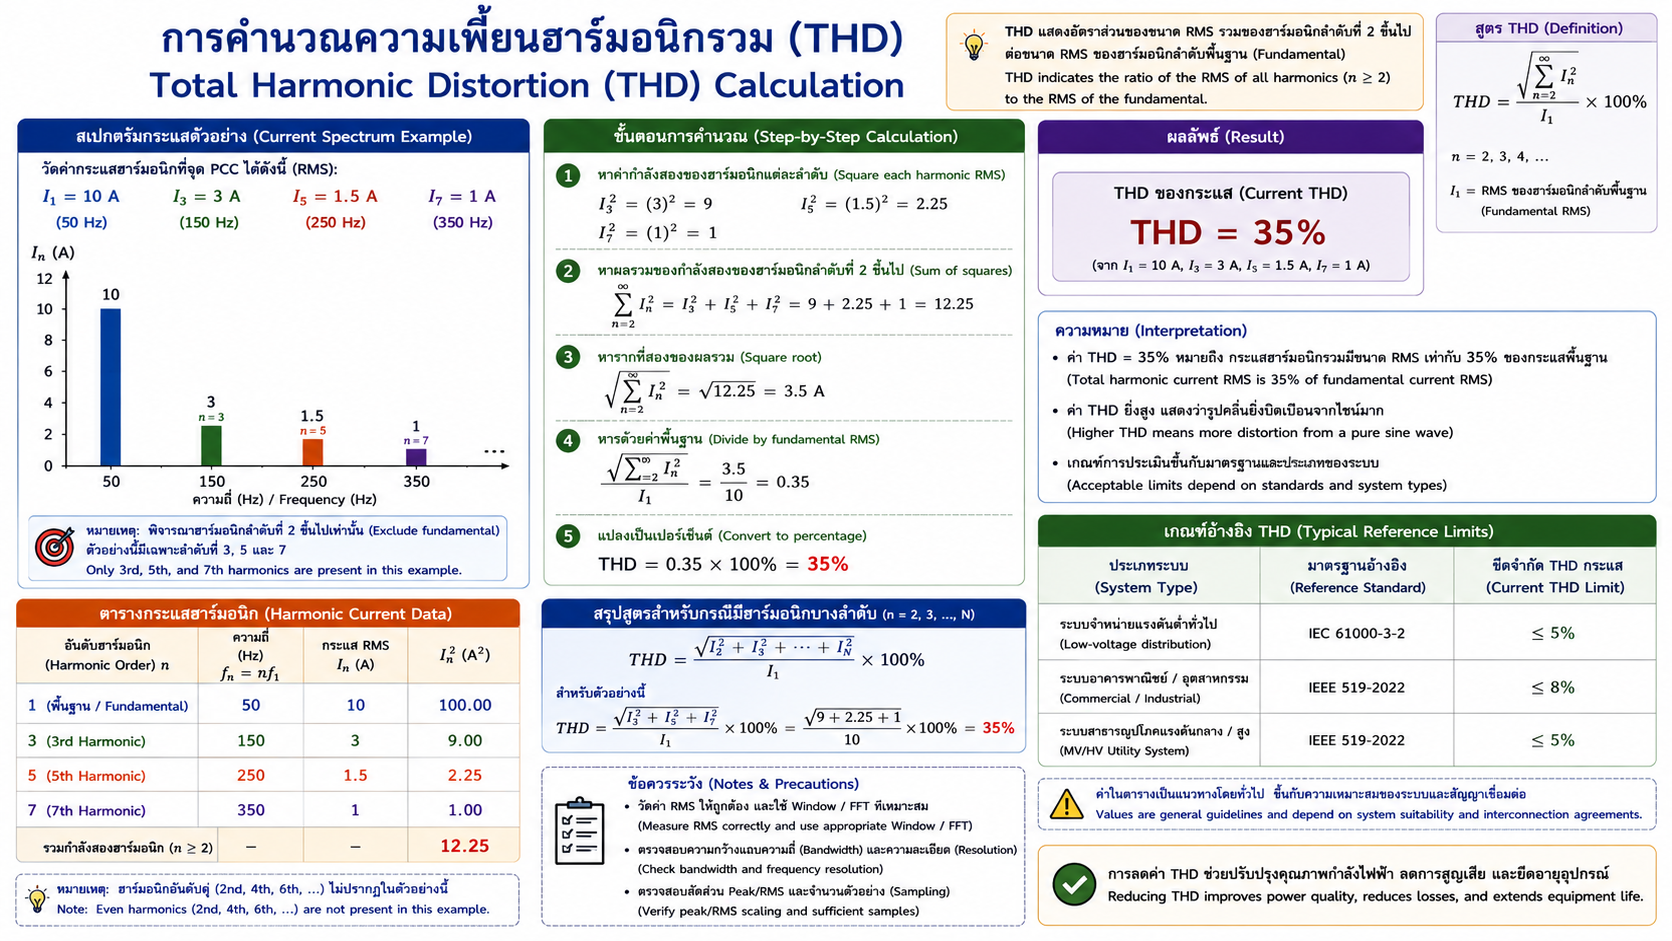
\includegraphics[width=0.8\textwidth]{images/chapter5/figure-06.png}
    \caption{การคำนวณ THD จากสเปกตรัม}
\end{figure}



\subsection{7.8 ผลกระทบของฮาร์มอนิกต่อระบบไฟฟ้า}

ฮาร์มอนิกไม่ได้ทำให้เกิดผลเสียเหมือนกันทุกระบบ ผลกระทบขึ้นกับขนาดฮาร์มอนิก อิมพีแดนซ์ของระบบ โครงสร้างสามเฟส อุปกรณ์ที่ต่อร่วม และตำแหน่งวัด การวิเคราะห์ที่ดีต้องพิจารณา “แหล่งกำเนิด–เส้นทาง–อุปกรณ์ที่รับผล” ร่วมกัน

\subsubsection{7.8.1 การสูญเสียและความร้อนเพิ่มขึ้น}

กระแส RMS ที่เพิ่มจากฮาร์มอนิกทำให้การสูญเสียแบบ $I^2R$ ในสายและขดลวดเพิ่มขึ้น

\[
P_{\mathrm{cu}}\approx I_{\mathrm{rms}}^2R
\]

อย่างไรก็ตาม ในความถี่สูง effective resistance อาจเพิ่มขึ้นจาก skin effect และ proximity effect ทำให้การสูญเสียจริงสูงกว่าการประมาณด้วย $R$ คงที่

\subsubsection{7.8.2 หม้อแปลง}

ฮาร์มอนิกสามารถเพิ่ม copper loss, eddy-current loss และความร้อนของหม้อแปลง โดยเฉพาะเมื่อมีกระแสฮาร์มอนิกความถี่สูง ในการใช้งานจริงจึงต้องพิจารณาการออกแบบและ derating ตามประเภทหม้อแปลงและข้อกำหนดที่เกี่ยวข้อง ไม่ควรใช้เพียงค่า THD เดียวตัดสิน

\subsubsection{7.8.3 สายนิวทรัลในระบบสามเฟสสี่สาย}

ฮาร์มอนิกลำดับที่เป็นสามเท่า เช่น 3, 9, 15 หรือ \textbf{triplen harmonics} มีลักษณะเฟสที่สามารถรวมกันในสายนิวทรัลแทนที่จะหักล้างเหมือน fundamental ของโหลดสามเฟสสมดุลบางกรณี จึงอาจทำให้กระแสนิวทรัลสูงอย่างไม่คาดคิดในระบบที่มีโหลดอิเล็กทรอนิกส์เฟสเดียวจำนวนมาก

\subsubsection{7.8.4 ตัวเก็บประจุและเรโซแนนซ์}

รีแอกแตนซ์ของตัวเก็บประจุลดลงเมื่อความถี่สูงขึ้น

\[
X_C=\frac{1}{2\pi fC}
\]

ขณะที่รีแอกแตนซ์ของตัวเหนี่ยวนำเพิ่มขึ้น

\[
X_L=2\pi fL
\]

เมื่อระบบมี L และ C อาจเกิด resonance ใกล้ความถี่ฮาร์มอนิก ทำให้กระแสหรือแรงดันบางความถี่ถูกขยาย ดังนั้นการติดตั้ง capacitor bank เพื่อแก้ power factor โดยไม่ประเมินฮาร์มอนิกและ resonance อาจสร้างปัญหาใหม่ได้

\subsubsection{7.8.5 มอเตอร์และเครื่องจักรไฟฟ้า}

ฮาร์มอนิกของแรงดันสามารถสร้างสนามแม่เหล็กและ torque pulsation เพิ่ม loss และ vibration ในเครื่องจักรไฟฟ้า ผลกระทบขึ้นกับ harmonic sequence และโครงสร้างของมอเตอร์

\subsubsection{7.8.6 อุปกรณ์ป้องกันและเครื่องมือวัด}

รูปคลื่นที่เพี้ยนอาจทำให้อุปกรณ์ที่ไม่ได้ออกแบบสำหรับ true RMS อ่านค่าไม่ถูกต้อง และอาจมีผลต่อการทำงานของอุปกรณ์ป้องกันบางชนิด การวัดเชิงคุณภาพกำลังจึงต้องใช้เครื่องมือและวิธีวัดที่เหมาะสม

\subsubsection{7.8.7 การรบกวนและการทำงานร่วมกันของอุปกรณ์}

ฮาร์มอนิกและองค์ประกอบความถี่สูงสามารถทำให้เกิดการรบกวนทางแม่เหล็กไฟฟ้าและปัญหาการทำงานร่วมกัน โดยเฉพาะเมื่อเส้นทางสายกำลังและสายสัญญาณอยู่ใกล้กัน แต่ต้องแยกปรากฏการณ์ low-frequency harmonics ออกจาก transient และ conducted/radiated EMI ที่มีช่วงความถี่ต่างกัน

\subsubsection{ตารางสรุปผลกระทบ}

\begin{table}[htbp]
    \centering
    \small
    \begin{tabularx}{\textwidth}{>{\raggedright\arraybackslash}p{0.16\textwidth} >{\raggedright\arraybackslash}X >{\raggedright\arraybackslash}X >{\raggedright\arraybackslash}X}
        \hline
        \textbf{อุปกรณ์/บริเวณ} & \textbf{กลไกหลัก} & \textbf{อาการที่อาจพบ} & \textbf{สิ่งที่ควรตรวจสอบ} \\
        \hline
        สายไฟ & RMS สูง, skin/proximity effect & ร้อน, สูญเสียเพิ่ม & RMS, harmonic spectrum, อุณหภูมิ \\
        สายนิวทรัล & triplen harmonics รวมกัน & กระแสนิวทรัลสูง & 3rd/9th/15th harmonic \\
        หม้อแปลง & copper/eddy loss & ความร้อน, อายุฉนวนลด & spectrum, loading, derating \\
        Capacitor bank & resonance / current amplification & กระแสสูง, fuse ขาด, capacitor เสีย & system impedance, resonant frequency \\
        มอเตอร์ & harmonic fields & loss, vibration, torque ripple & voltage spectrum, motor current \\
        เครื่องมือวัด & waveform sensitivity & ค่าอ่านคลาดเคลื่อน & true-RMS capability, bandwidth \\
        \hline
    \end{tabularx}
\end{table}

% [รูปที่ 7: ผลกระทบของฮาร์มอนิกต่อระบบไฟฟ้า]
% ประเภทภาพ: Technical Infographic
% ตำแหน่งที่แนะนำ: หัวข้อ 7.8
% วัตถุประสงค์การเรียนรู้: เชื่อมโยงฮาร์มอนิกกับอุปกรณ์ที่ได้รับผล
% คำอธิบายภาพ: single-line system แบบง่ายจาก PCC ไปยัง transformer, feeder, neutral, capacitor bank, motor และ electronic loads พร้อม callout ผลกระทบ
% องค์ประกอบที่ต้องมี: transformer, 3-phase 4-wire feeder, neutral, capacitor bank, motor, nonlinear loads
% ข้อความหรือป้ายกำกับ: “Heating”, “Neutral triplen current”, “Resonance”, “Torque ripple”, “Measurement error”
% ภาษาของป้ายกำกับ: ไทยและอังกฤษ
% สัดส่วนภาพ: 16:9
% Image Generation Prompt: Power-quality engineering infographic showing a simplified three-phase electrical distribution system with transformer, feeders, neutral conductor, capacitor bank, induction motor, and nonlinear electronic loads. Add callouts for harmonic effects: extra heating, triplen harmonic neutral current, capacitor resonance, motor torque ripple, and measurement error. White background, clean vector textbook style, bilingual Thai-English labels, 16:9.
% Alt Text: อินโฟกราฟิกระบบไฟฟ้าที่ชี้ผลของฮาร์มอนิกต่อสาย นิวทรัล หม้อแปลง capacitor bank มอเตอร์ และเครื่องมือวัด

\begin{figure}[htbp]
    \centering
    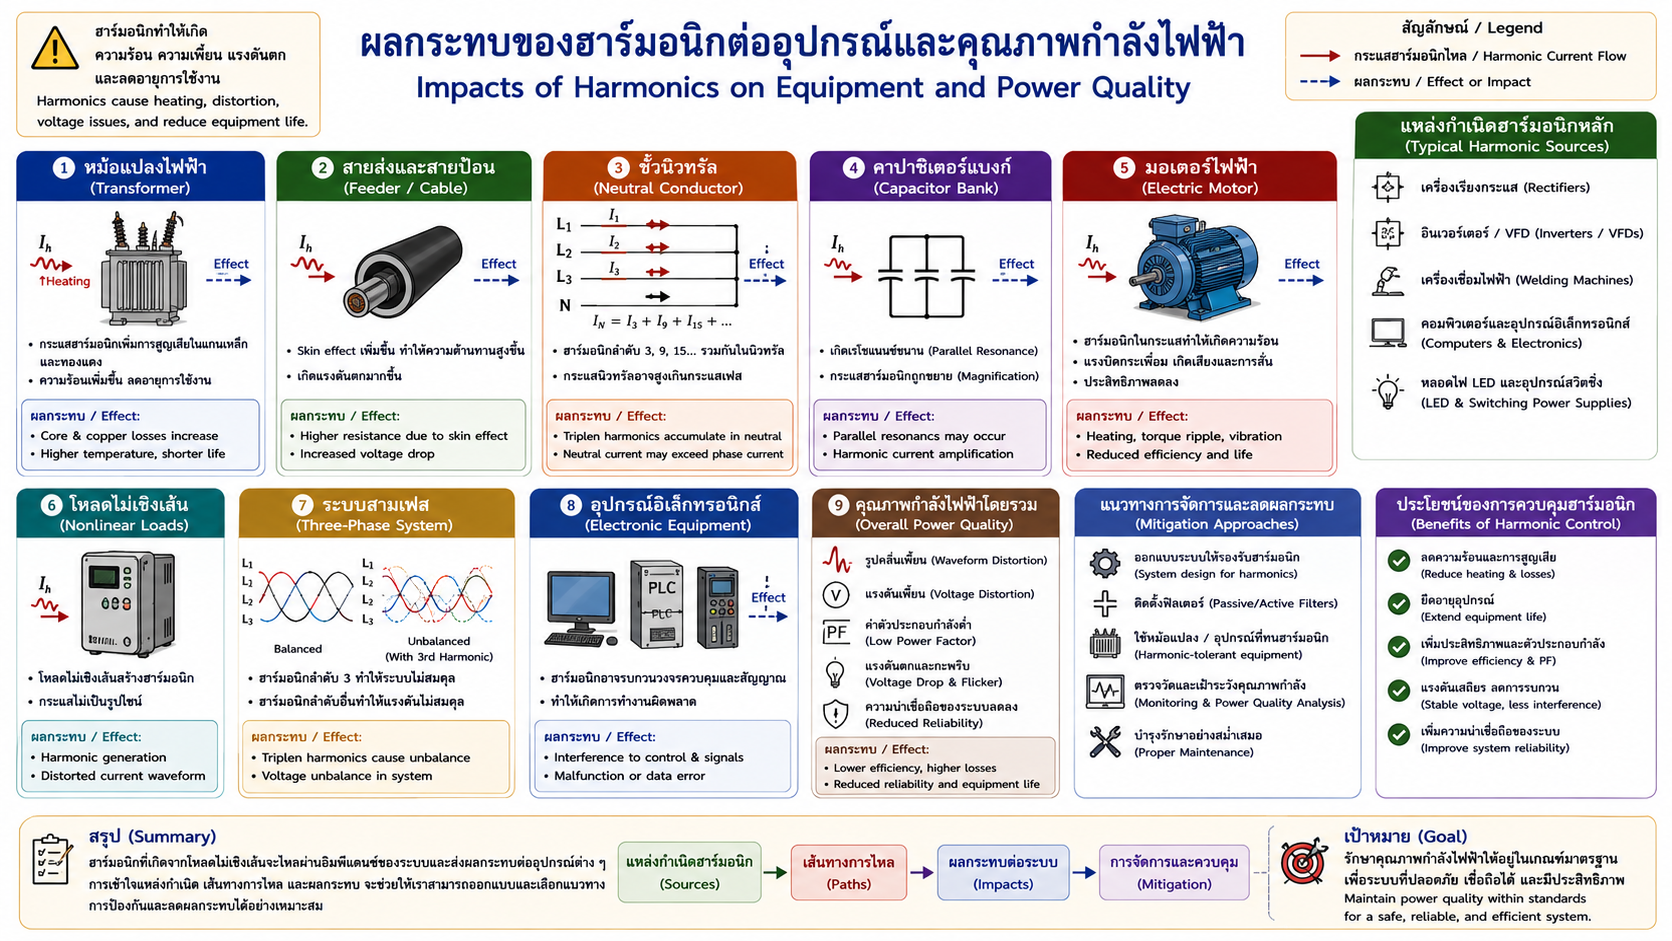
\includegraphics[width=0.8\textwidth]{images/chapter5/figure-07.png}
    \caption{ผลกระทบของฮาร์มอนิกต่อระบบไฟฟ้า}
\end{figure}



\subsection{7.9 การกรองสัญญาณและแนวคิดเบื้องต้นของฟิลเตอร์}

\subsubsection{7.9.1 เป้าหมายของการกรอง}

ฟิลเตอร์มีหน้าที่เลือกผ่านหรือลดทอนองค์ประกอบความถี่บางช่วง ในบริบทของฮาร์มอนิกอาจมีเป้าหมาย เช่น

\begin{itemize}
    \item รักษา fundamental 50 Hz แต่ลด 5th, 7th และฮาร์มอนิกลำดับสูง
    \item สร้างทางอิมพีแดนซ์ต่ำให้ฮาร์มอนิกเป้าหมายไหลผ่านแทนระบบ
    \item สร้างกระแสชดเชยที่มีขนาดเท่ากันแต่เฟสตรงข้ามกับฮาร์มอนิกของโหลด
\end{itemize}

\subsubsection{7.9.2 RC low-pass filter เพื่อเข้าใจแนวคิด}

วงจร RC low-pass มี transfer magnitude

\[
|H(j\omega)|=\frac{1}{\sqrt{1+(\omega RC)^2}}
\]

และความถี่ตัด

\[
f_c=\frac{1}{2\pi RC}
\]

\textbf{ที่มา:} ได้จาก voltage divider ระหว่าง $R$ และอิมพีแดนซ์ของตัวเก็บประจุ $Z_C=1/(j\omega C)$

\textbf{ความหมายทางกายภาพ:} ที่ความถี่ต่ำ capacitor มีอิมพีแดนซ์สูงและเอาต์พุตใกล้อินพุต ที่ความถี่สูง capacitor มีอิมพีแดนซ์ต่ำลงและสัญญาณเอาต์พุตถูกลดทอน

\textbf{ข้อจำกัด:} RC filter เหมาะสำหรับสัญญาณกำลังต่ำหรือวงจรสัญญาณ ไม่ควรนำค่าตัวอย่างไปต่อกับระบบไฟฟ้ากำลังโดยตรงโดยไม่ออกแบบพิกัดแรงดัน กระแส กำลัง และความปลอดภัย

\subsubsection{ตัวอย่างที่ 5: เปรียบเทียบการลดทอน fundamental กับ 5th harmonic}

\textbf{ตัวอย่างเพิ่มเติมเพื่อการเรียนรู้}

ออกแบบเชิงการเรียนรู้ให้ RC low-pass มี $f_c\approx100$ Hz โดยเลือก

\[
R=15.9\ \Omega,\qquad C=100\ \mu\mathrm{F}
\]

ตรวจสอบ

\[
f_c=\frac{1}{2\pi(15.9)(100\times10^{-6})}\approx100.1\ \text{Hz}
\]

สำหรับ 50 Hz

\[
|H(50)|=\frac{1}{\sqrt{1+(50/100.1)^2}}\approx0.895
\]

สำหรับ 5th harmonic ที่ 250 Hz

\[
|H(250)|=\frac{1}{\sqrt{1+(250/100.1)^2}}\approx0.372
\]

\textbf{การแปลความหมาย:} filter นี้ลด fundamental เหลือประมาณ 89.5\% แต่ลด 5th harmonic เหลือประมาณ 37.2\% จึงแสดงหลักการ “ความถี่สูงถูกลดทอนมากกว่า” แต่ยังไม่ใช่การออกแบบ power harmonic filter ที่เหมาะสม เพราะ fundamental ถูกลดทอนมากเกินไปและไม่ได้พิจารณาพิกัดกำลัง

\subsubsection{7.9.3 LC tuned filter}

วงจร L-C มีความถี่เรโซแนนซ์เชิงอุดมคติ

\[
f_r=\frac{1}{2\pi\sqrt{LC}}
\]

ถ้าต้องการ tune ใกล้ 5th harmonic ของ 50 Hz จะมี

\[
f_r\approx250\ \text{Hz}
\]

ตัวอย่าง หากเลือก $C=20\ \mu\mathrm{F}$

\[
L=\frac{1}{(2\pi f_r)^2C}
\]

\[
L\approx20.3\ \text{mH}
\]

ในระบบจริงต้องมีการพิจารณา damping, component tolerance, reactive power, system impedance, detuning และ resonance กับระบบ จึงไม่ควรใช้สมการอุดมคติเพียงสมการเดียวเพื่อสร้างฟิลเตอร์กำลังจริง

\subsubsection{7.9.4 Passive harmonic filter}

ฟิลเตอร์พาสซีฟในระบบกำลังอาจใช้แขนง RLC ที่ tune ใกล้ฮาร์มอนิกเป้าหมายเพื่อสร้างเส้นทางอิมพีแดนซ์ต่ำให้กระแสฮาร์มอนิก หรือใช้ high-pass configuration สำหรับฮาร์มอนิกลำดับสูง ข้อดีคือโครงสร้างไม่ซับซ้อนและไม่ต้องมีวงจรควบคุมความเร็วสูง แต่การทำงานขึ้นกับอิมพีแดนซ์ของระบบและอาจมีปัญหา resonance หรือ detuning

\subsubsection{7.9.5 Active power filter}

Active power filter วัดกระแสหรือแรงดันของระบบ ประเมินส่วนที่ต้องการชดเชย แล้วใช้อุปกรณ์อิเล็กทรอนิกส์กำลังสร้างกระแสชดเชย ตัวอย่างแนวคิด

\[
i_s(t)=i_L(t)-i_c(t)
\]

ถ้า $i_c(t)$ ถูกสร้างให้ใกล้เคียงส่วนฮาร์มอนิกของโหลด กระแสด้านแหล่งจ่าย $i_s(t)$ จะเข้าใกล้รูปคลื่น fundamental มากขึ้น

\subsubsection{7.9.6 เปรียบเทียบแนวทางกรอง}

\begin{table}[htbp]
    \centering
    \small
    \begin{tabularx}{\textwidth}{>{\raggedright\arraybackslash}p{0.20\textwidth} >{\raggedright\arraybackslash}X >{\raggedright\arraybackslash}X >{\raggedright\arraybackslash}X}
        \hline
        \textbf{แนวทาง} & \textbf{หลักการ} & \textbf{ข้อดี} & \textbf{ข้อจำกัด} \\
        \hline
        RC/LC low-pass & ลดความถี่สูง & เข้าใจง่าย & อาจลด fundamental, ต้องออกแบบพิกัด \\
        Tuned passive filter & สร้าง low impedance ที่ฮาร์มอนิกเป้าหมาย & โครงสร้างไม่ซับซ้อน & detuning/resonance, ไวต่อระบบ \\
        High-pass passive & ระบายฮาร์มอนิกลำดับสูง & ครอบคลุมช่วงกว้างขึ้น & loss และการเลือกค่า RLC \\
        Active power filter & ฉีดกระแสชดเชย & ปรับตามโหลดได้ & ราคาและระบบควบคุมซับซ้อน \\
        \hline
    \end{tabularx}
\end{table}

% [รูปที่ 8: เปรียบเทียบฟิลเตอร์พาสซีฟและแอ็กทีฟสำหรับฮาร์มอนิก]
% ประเภทภาพ: Block Diagram / Technical Illustration
% ตำแหน่งที่แนะนำ: หลังหัวข้อ 7.9.6
% วัตถุประสงค์การเรียนรู้: เปรียบเทียบกลไกการลดฮาร์มอนิกสองแนวทาง
% คำอธิบายภาพ: ซ้ายเป็น shunt passive tuned filter ต่อที่ PCC ขวาเป็น active filter วัดโหลดและฉีด compensating current
% องค์ประกอบที่ต้องมี: source, PCC, nonlinear load, RLC branch, current sensor, active converter, compensation current arrow
% ข้อความหรือป้ายกำกับ: “Passive tuned path”, “Active compensation”, “Harmonic current”
% ภาษาของป้ายกำกับ: ไทยและอังกฤษ
% สัดส่วนภาพ: 16:9
% Image Generation Prompt: Side-by-side electrical engineering diagram comparing passive and active harmonic filtering. Left: AC source, PCC, nonlinear load, and a shunt tuned RLC harmonic filter providing a low-impedance path for harmonic current. Right: AC source, PCC, nonlinear load, current sensor, active power filter converter injecting compensating current opposite to the harmonic current. White background, bilingual Thai-English labels, clean vector textbook style, 16:9.
% Alt Text: แผนภาพเปรียบเทียบ passive filter ที่ระบายฮาร์มอนิกผ่านวงจร RLC กับ active filter ที่ฉีดกระแสชดเชย

\begin{figure}[htbp]
    \centering
    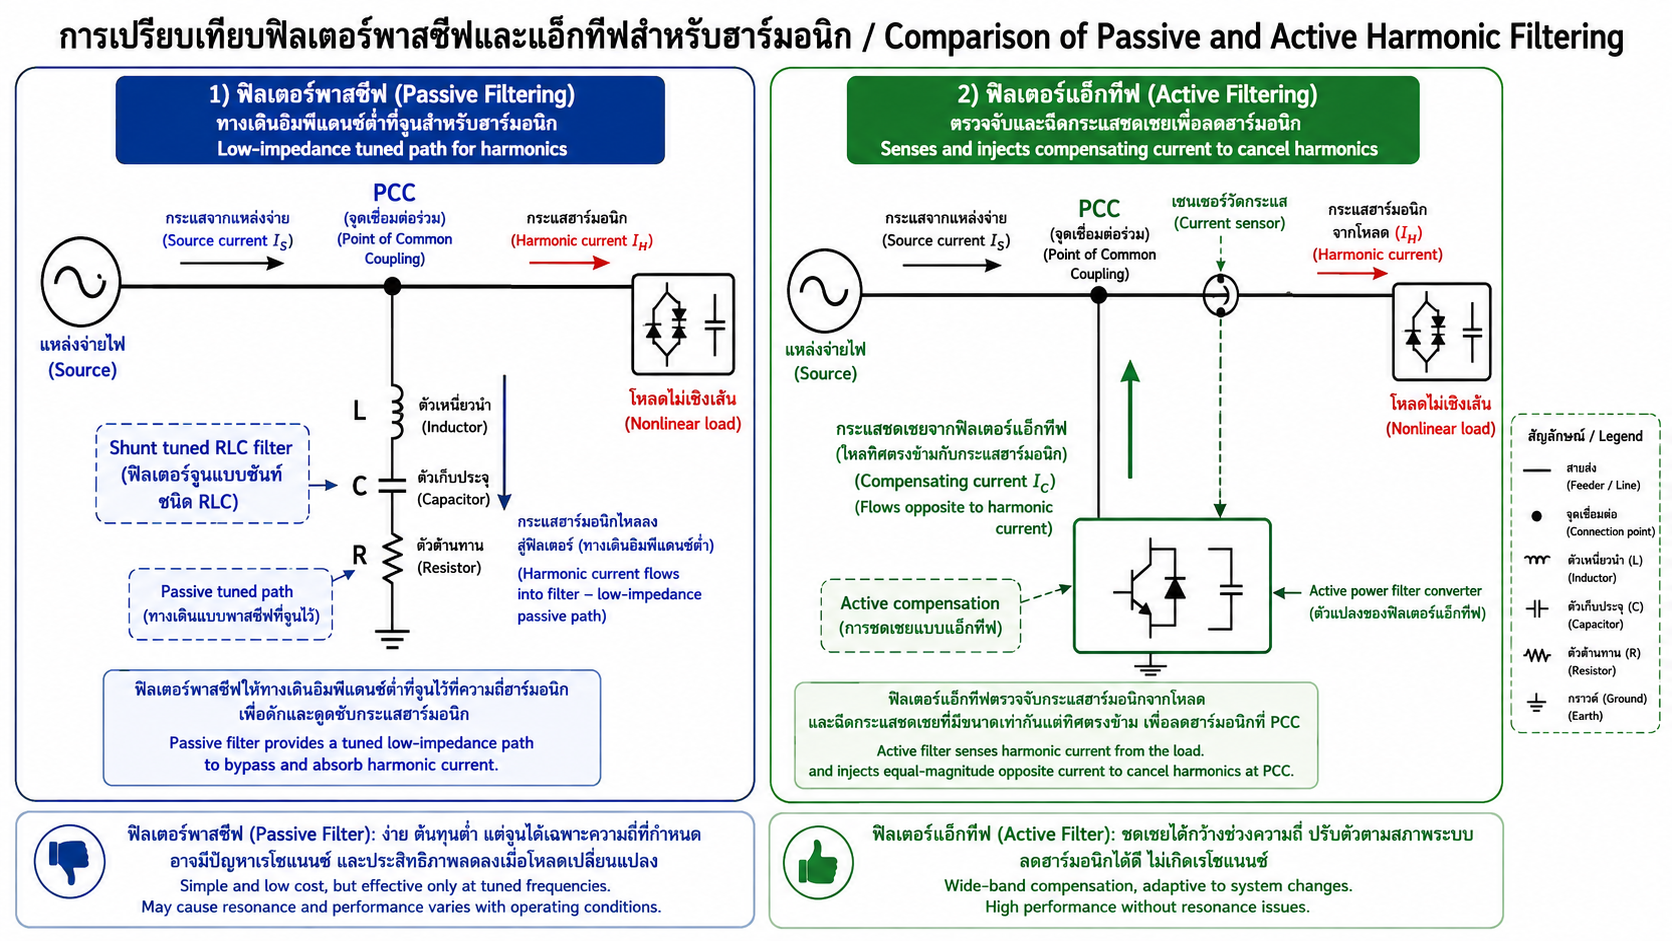
\includegraphics[width=0.8\textwidth]{images/chapter5/figure-08.png}
    \caption{เปรียบเทียบฟิลเตอร์พาสซีฟและแอ็กทีฟสำหรับฮาร์มอนิก}
\end{figure}



\subsection{7.10 การใช้โปรแกรมคำนวณวิเคราะห์รูปคลื่นไฟฟ้า}

หัวข้อนี้ใช้โปรแกรมเป็นเครื่องมือ \textbf{ตรวจสอบแนวคิดคณิตศาสตร์} ไม่ใช่แทนที่ความเข้าใจ ผู้เรียนควรรู้ก่อนว่า FFT ให้ข้อมูลอะไร ขนาดสเปกตรัมถูก normalize อย่างไร และความละเอียดความถี่สัมพันธ์กับเวลาบันทึกสัญญาณอย่างไร

\subsubsection{7.10.1 จากสัญญาณต่อเนื่องสู่ข้อมูลตัวอย่าง}

ให้ sample สัญญาณด้วยอัตรา

\[
f_s=\frac{1}{\Delta t}
\]

ถ้ามีตัวอย่าง $N$ จุด ระยะเวลาบันทึกประมาณ

\[
T_{\mathrm{obs}}=\frac{N}{f_s}
\]

และ frequency-bin spacing ของ DFT คือ

\[
\Delta f=\frac{f_s}{N}=\frac{1}{T_{\mathrm{obs}}}
\]

ดังนั้น หากต้องการแยกความถี่ที่อยู่ใกล้กันมาก ต้องเพิ่มเวลาบันทึก ไม่ใช่เพียงเพิ่ม sampling rate อย่างเดียว

\subsubsection{7.10.2 Sampling และ Nyquist consideration}

ความถี่สูงสุดที่แทนได้โดยไม่เกิด aliasing ภายใต้เงื่อนไข sampling อุดมคติคือ

\[
f_{\mathrm{Nyquist}}=\frac{f_s}{2}
\]

ในระบบวัดจริงยังต้องพิจารณา anti-alias filter, bandwidth ของ sensor และเครื่องมือวัด

\subsubsection{7.10.3 Spectral leakage}

ถ้าช่วงข้อมูลที่เลือกไม่ประกอบด้วยจำนวนคาบที่เหมาะสม พลังงานของไซน์หนึ่งความถี่อาจกระจายไปหลาย frequency bins เรียกว่า \textbf{spectral leakage} การใช้ window ช่วยลด leakage บางลักษณะ แต่ทำให้ main lobe กว้างขึ้นและมีผลต่อ amplitude estimation ดังนั้นผู้เรียนควรเรียนรู้ว่า “FFT plot” ขึ้นกับวิธีเก็บข้อมูลและประมวลผล ไม่ใช่ความจริงที่ไม่ต้องตีความ

\subsubsection{7.10.4 ตัวอย่าง Python: สร้างรูปคลื่นและคำนวณ FFT}

ตัวอย่างต่อไปนี้ใช้ NumPy และ Matplotlib โดยสร้างสัญญาณ 50 Hz ที่มี 3rd และ 5th harmonic

\begin{verbatim}
import numpy as np
import matplotlib.pyplot as plt

fs = 10000.0          # sampling frequency, Hz
Tobs = 0.2            # observation time, s
N = int(fs * Tobs)
t = np.arange(N) / fs

# RMS amplitudes
I1 = 10.0
I3 = 3.0
I5 = 1.5

# Convert RMS amplitude to peak with sqrt(2)
i = (np.sqrt(2)*I1*np.sin(2*np.pi*50*t)
     + np.sqrt(2)*I3*np.sin(2*np.pi*150*t - np.deg2rad(20))
     + np.sqrt(2)*I5*np.sin(2*np.pi*250*t + np.deg2rad(30)))

# One-sided FFT for real-valued input
Y = np.fft.rfft(i)
f = np.fft.rfftfreq(N, d=1/fs)

# Convert two-sided-equivalent FFT coefficient to peak amplitude
Apeak = 2*np.abs(Y) / N
Apeak[0] = np.abs(Y[0]) / N

# Convert sinusoidal peak amplitudes to RMS
Arms = Apeak / np.sqrt(2)
Arms[0] = Apeak[0]   # DC RMS equals DC magnitude

plt.figure()
plt.plot(t*1000, i)
plt.xlim(0, 40)
plt.xlabel('Time (ms)')
plt.ylabel('Current (A)')
plt.title('Distorted current waveform')
plt.grid(True)

plt.figure()
mask = f <= 500
plt.stem(f[mask], Arms[mask])
plt.xlabel('Frequency (Hz)')
plt.ylabel('RMS magnitude (A)')
plt.title('One-sided RMS spectrum')
plt.grid(True)
plt.show()
\end{verbatim}

\textbf{สิ่งที่ควรสังเกต}

\begin{itemize}
    \item $f_s=10$ kHz
    \item $T_{\mathrm{obs}}=0.2$ s
    \item $N=2000$
    \item ความละเอียดความถี่
\end{itemize}

\[
\Delta f=\frac{10000}{2000}=5\ \text{Hz}
\]

ดังนั้น 50, 150 และ 250 Hz อยู่ตรงกับ frequency bins พอดีในตัวอย่างนี้ ทำให้การอ่านแอมพลิจูดตรงไปตรงมา

\subsubsection{7.10.5 คำนวณ THD จากค่าฮาร์มอนิกใน Python}

ถ้าทราบ RMS harmonic magnitudes แล้ว สามารถคำนวณโดยตรง

\begin{verbatim}
I1 = 10.0
harmonics = np.array([3.0, 1.5, 1.0])
thd = np.sqrt(np.sum(harmonics**2)) / I1
print(f"THD = {100*thd:.2f}%")
\end{verbatim}

ผลที่คาดหวังคือ

\begin{verbatim}
THD = 35.00%
\end{verbatim}

\subsubsection{7.10.6 ตัวอย่าง MATLAB/Octave แนวคิดเดียวกัน}

\begin{verbatim}
fs = 10000;
Tobs = 0.2;
N = fs*Tobs;
t = (0:N-1)/fs;

i = sqrt(2)*10*sin(2*pi*50*t) ...
  + sqrt(2)*3*sin(2*pi*150*t - deg2rad(20)) ...
  + sqrt(2)*1.5*sin(2*pi*250*t + deg2rad(30));

Y = fft(i);
f = (0:N-1)*(fs/N);

Apeak = 2*abs(Y)/N;
Arms = Apeak/sqrt(2);

idx = f <= 500;
stem(f(idx), Arms(idx));
xlabel('Frequency (Hz)');
ylabel('Approx. RMS magnitude (A)');
grid on;
\end{verbatim}

\textbf{หมายเหตุ:} ในการใช้งานจริงต้องจัดการ one-sided spectrum, DC, Nyquist bin, window scaling และ normalization อย่างถูกต้อง การใช้ฟังก์ชันสำเร็จรูปสำหรับ THD อาจใช้วิธีประเมินสเปกตรัมหรือจำนวนฮาร์มอนิกต่างจากสูตรที่คำนวณด้วยมือ ผู้เรียนควรอ่านเอกสารฟังก์ชันของเวอร์ชันซอฟต์แวร์ที่ใช้และระบุวิธีคำนวณในรายงาน

\subsubsection{7.10.7 กระบวนการวิเคราะห์ FFT ที่แนะนำ}

\begin{enumerate}
    \item ระบุชนิดสัญญาณและหน่วย
    \item ทราบหรือประมาณ $f_0$
    \item เลือก $f_s$ ให้สูงพอสำหรับความถี่สูงสุดที่สนใจ
    \item เลือกช่วงข้อมูลที่เป็น steady state
    \item ตรวจสอบจำนวนคาบในช่วงข้อมูล
    \item เลือก window หากจำเป็น
    \item คำนวณ FFT/DFT
    \item normalize amplitude อย่างถูกต้อง
    \item แปลง peak $\leftrightarrow$ RMS ให้ชัดเจน
    \item ระบุ harmonic bins หรือใช้ peak detection อย่างมีหลักเกณฑ์
    \item คำนวณ THD
    \item เปรียบเทียบผลกับการคำนวณเชิงทฤษฎีหรือข้อมูลเครื่องมือวัด
\end{enumerate}

% [รูปที่ 9: ขั้นตอนการวิเคราะห์ฮาร์มอนิกด้วย FFT]
% ประเภทภาพ: Flowchart
% ตำแหน่งที่แนะนำ: หลังหัวข้อ 7.10.7
% วัตถุประสงค์การเรียนรู้: ให้ผู้เรียนเห็น workflow ที่ถูกต้องตั้งแต่การเก็บข้อมูลถึงการตีความ THD
% คำอธิบายภาพ: flowchart 8–10 ขั้น จาก waveform acquisition → sampling → steady-state window → FFT → normalization → spectrum → harmonic extraction → RMS/THD → validation
% องค์ประกอบที่ต้องมี: sampling rate, observation time, window, FFT, frequency bins, RMS, THD, validation
% ข้อความหรือป้ายกำกับ: “Avoid aliasing”, “Check leakage”, “Peak or RMS?”, “Validate with theory”
% ภาษาของป้ายกำกับ: ไทยและอังกฤษ
% สัดส่วนภาพ: 16:9
% Image Generation Prompt: Engineering education flowchart for harmonic analysis using FFT. Steps: acquire waveform, choose sampling frequency, select steady-state observation window, check number of cycles, apply window if needed, compute FFT, normalize one-sided spectrum, convert amplitude to RMS, identify harmonic orders, calculate THD, validate against theory. Include warning callouts for aliasing, spectral leakage, and peak-vs-RMS scaling. White background, bilingual Thai-English labels, clean vector style, 16:9.
% Alt Text: ผังงานวิเคราะห์ FFT ตั้งแต่การเก็บข้อมูล เลือก sampling และ window ไปจนถึงการหาสเปกตรัม RMS และ THD พร้อมตรวจสอบ aliasing และ leakage

\begin{figure}[htbp]
    \centering
    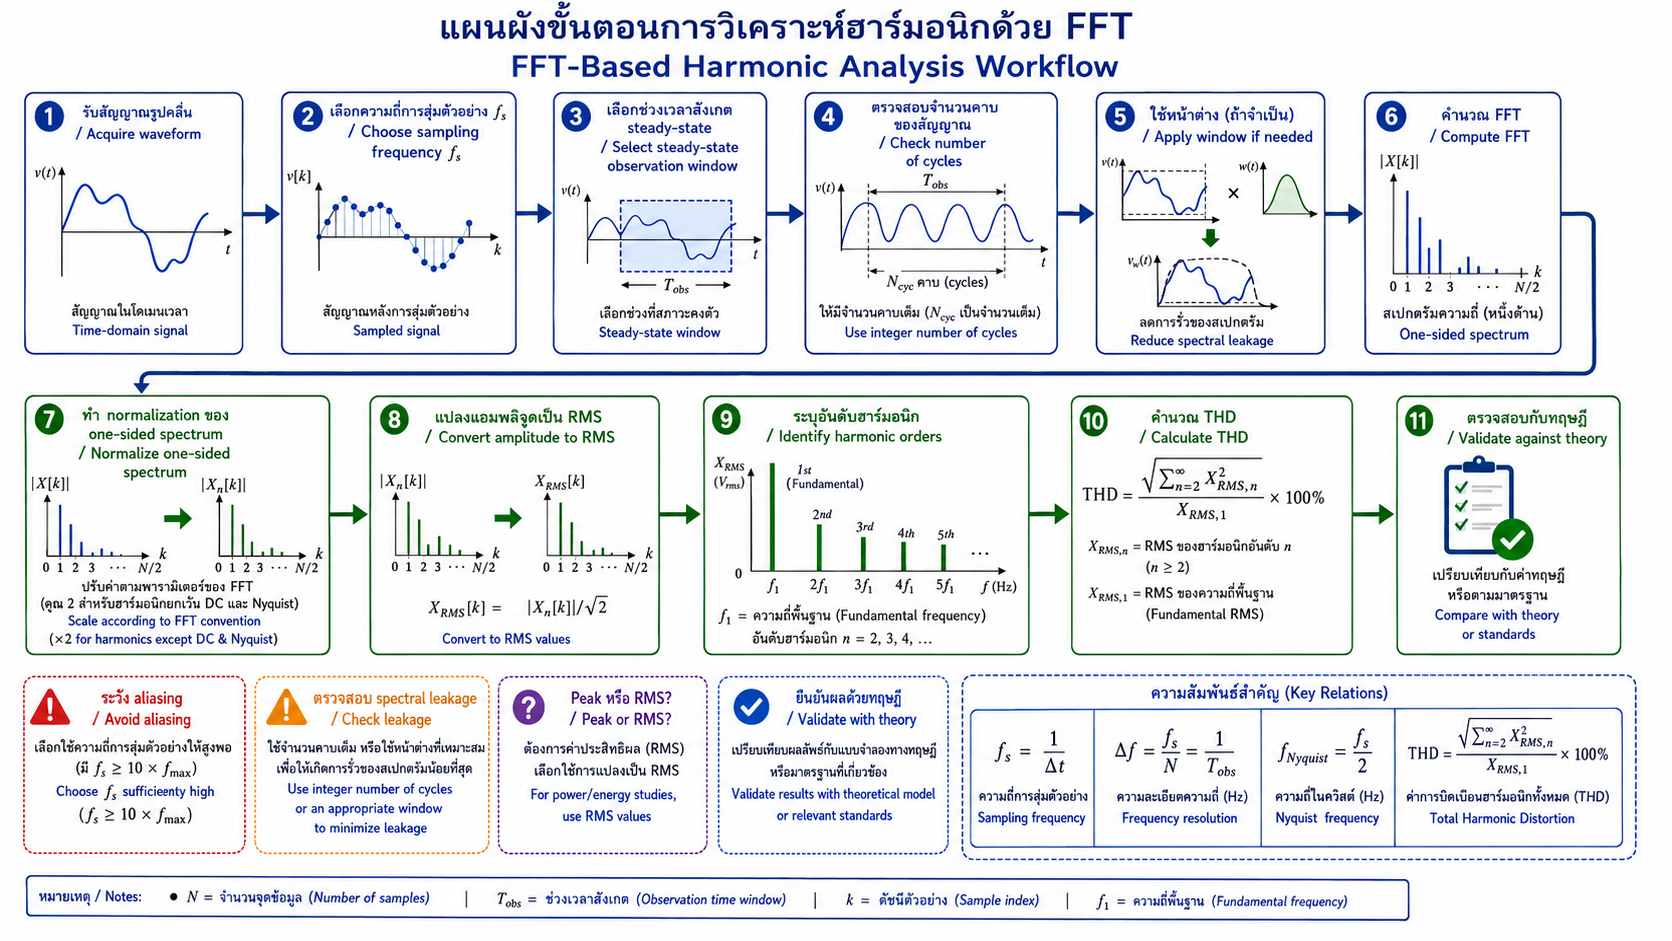
\includegraphics[width=0.8\textwidth]{images/chapter5/figure-09.png}
    \caption{ขั้นตอนการวิเคราะห์ฮาร์มอนิกด้วย FFT}
\end{figure}



\subsection{7.11 ตัวอย่างโจทย์และการคำนวณแบบเป็นขั้นตอน}

หัวข้อนี้รวบรวมตัวอย่างประยุกต์ที่เชื่อม RMS, THD, กำลัง และฟิลเตอร์เข้าด้วยกัน

\subsubsection{ตัวอย่างที่ 6: จาก THD ไปสู่กระแส RMS และ true PF}

\textbf{ตัวอย่างเพิ่มเติมเพื่อการเรียนรู้}

โหลดเฟสเดียวรับแรงดันไซน์บริสุทธิ์ 230 V RMS ดึง fundamental current 12 A RMS มี $\mathrm{THD}_I=40\%$ และ displacement factor ที่ fundamental เท่ากับ 0.95 จงหา

\begin{enumerate}
    \item กระแส RMS รวม
    \item กำลังจริง
    \item apparent power
    \item true PF
\end{enumerate}

\textbf{ขั้นที่ 1 กำหนดตัวแปร}

\[
\begin{aligned}
    V_1=230\ \text{V},\quad I_1=12\ \text{A},\quad \mathrm{THD}_I=0.40, \\
    \quad \cos\phi_1=0.95
\end{aligned}
\]

\textbf{ขั้นที่ 2 หา RMS รวม}

\[
I_{\mathrm{rms}}=I_1\sqrt{1+\mathrm{THD}_I^2}
\]

\[
=12\sqrt{1+0.4^2}
\]

\[
=12\sqrt{1.16}=12.92\ \text{A}
\]

\textbf{ขั้นที่ 3 หากำลังจริง}

แรงดันเป็นไซน์บริสุทธิ์ จึงมีเพียง fundamental voltage

\[
P=V_1I_1\cos\phi_1
\]

\[
=230(12)(0.95)=2622\ \text{W}
\]

\textbf{ขั้นที่ 4 หา apparent power}

\[
S=V_{\mathrm{rms}}I_{\mathrm{rms}}=230(12.92)=2971.6\ \text{VA}
\]

\textbf{ขั้นที่ 5 หา true PF}

\[
PF=\frac{2622}{2971.6}=0.882
\]

\textbf{ขั้นที่ 6 ตรวจสอบทางเลือก}

\[
\begin{aligned}
    \frac{I_1}{I_{\mathrm{rms}}}\cos\phi_1 \\
    =\frac{12}{12.92}(0.95)\approx0.882
\end{aligned}
\]

ตรงกัน

\textbf{คำตอบ}

\[
\boxed{I_{\mathrm{rms}}\approx12.92\ \text{A},\quad P\approx2.622\ \text{kW},\quad S\approx2.972\ \text{kVA},\quad PF\approx0.882}
\]

\subsubsection{ตัวอย่างที่ 7: วิเคราะห์ว่าฮาร์มอนิกลำดับใดควรให้ความสำคัญ}

\textbf{ตัวอย่างเพิ่มเติมเพื่อการเรียนรู้}

วัดกระแสโหลดได้

\begin{table}[htbp]
    \centering
    \begin{tabular}{r r}
        \hline
        \textbf{Harmonic} & \textbf{RMS current} \\
        \hline
        1 & 20 A \\
        3 & 8 A \\
        5 & 2 A \\
        7 & 1.5 A \\
        9 & 3 A \\
        \hline
    \end{tabular}
\end{table}

จงจัดลำดับความสำคัญของฮาร์มอนิกสำหรับการวิเคราะห์

\textbf{ขั้นที่ 1 คำนวณสัดส่วนเทียบ fundamental}

\[
I_3/I_1=8/20=40\%
\]

\[
I_5/I_1=10\%,\quad I_7/I_1=7.5\%,\quad I_9/I_1=15\%
\]

\textbf{ขั้นที่ 2 พิจารณาบริบท} \\
ถ้าเป็นระบบสามเฟสสี่สายที่มีโหลดเฟสเดียวจำนวนมาก 3rd และ 9th เป็น triplen harmonics จึงควรตรวจสอบสายนิวทรัลเป็นพิเศษ

\textbf{ขั้นที่ 3 สรุป} \\
3rd harmonic มีขนาดสูงสุดและมีนัยสำคัญทั้งด้าน THD และ neutral current ส่วน 9th แม้ต่ำกว่า 5th ในบางระบบทั่วไป แต่มีลักษณะ triplen จึงควรให้ความสำคัญเชิงโครงสร้างระบบ

\textbf{ข้อสังเกต:} การจัดลำดับจาก “ขนาด” เพียงอย่างเดียวไม่พอ ต้องพิจารณาคุณสมบัติของ harmonic order และอุปกรณ์ในระบบด้วย

\subsubsection{ตัวอย่างที่ 8: ประเมิน tuned frequency ของฟิลเตอร์}

\textbf{ตัวอย่างเพิ่มเติมเพื่อการเรียนรู้}

ระบบ 50 Hz พบ 5th harmonic เด่น ต้องการใช้แบบจำลอง LC เพื่อเรียนรู้การ tune ใกล้ 250 Hz หาก $C=20\ \mu$F จงหา $L$

\textbf{ขั้นที่ 1 ความถี่เป้าหมาย}

\[
f_5=5f_0=5(50)=250\ \text{Hz}
\]

\textbf{ขั้นที่ 2 ใช้สมการ resonance}

\[
f_r=\frac{1}{2\pi\sqrt{LC}}
\]

จัดรูป

\[
L=\frac{1}{(2\pi f_r)^2C}
\]

\textbf{ขั้นที่ 3 แทนค่า}

\[
L=\frac{1}{(2\pi\times250)^2(20\times10^{-6})}
\]

\[
L\approx0.0203\ \text{H}=20.3\ \text{mH}
\]

\textbf{ขั้นที่ 4 แปลความหมายและข้อจำกัด} \\
ค่านี้เป็นค่าทางทฤษฎีของ LC อุดมคติ การออกแบบฟิลเตอร์จริงต้องพิจารณา R, Q-factor, tolerance, detuning, reactive power และ system resonance

\textbf{คำตอบ}

\[
\boxed{L\approx20.3\ \text{mH}}
\]



\subsection{7.12 กิจกรรมการเรียนรู้และแบบฝึกหัดท้ายบท}

รายละเอียดกิจกรรมและแบบฝึกหัดฉบับเต็มอยู่ในหัวข้อ 11–12 ของบท เพื่อให้สอดคล้องกับรูปแบบมาตรฐานของเอกสารประกอบการสอนทั้งรายวิชา โดยกิจกรรมจะเน้นการอ่านสเปกตรัม การคำนวณ RMS/THD การเชื่อมโยงฮาร์มอนิกกับ power quality และการตรวจสอบผลด้วยโปรแกรมคำนวณ



\subsection{8. ความเข้าใจผิดที่พบบ่อย}

\subsubsection{8.1 “THD ต่ำ แปลว่ารูปคลื่นดีทุกด้าน”}

ไม่ถูกต้อง THD วัดเฉพาะฮาร์มอนิกเทียบ fundamental และไม่บอก transient, flicker, unbalance, interharmonics หรือเฟสขององค์ประกอบ ความสมบูรณ์ของ power quality จึงต้องใช้พารามิเตอร์หลายชนิด

\subsubsection{8.2 “ฮาร์มอนิกลำดับที่ 5 คือความถี่ 5 Hz”}

ไม่ถูกต้อง harmonic order เป็น \textbf{ตัวคูณของ fundamental} ถ้า $f_0=50$ Hz, 5th harmonic คือ 250 Hz

\subsubsection{8.3 “RMS ของหลายฮาร์มอนิกบวกกันตรง ๆ”}

ไม่ถูกต้อง ต้องใช้ root-sum-square

\[
X_{\mathrm{rms}}=\sqrt{\sum X_n^2}
\]

เมื่อ $X_n$ เป็น RMS ขององค์ประกอบออร์โทโกนัล

\subsubsection[8.4 ถ้า cos phi1 = 1 ตัวประกอบกำลังรวมต้องเป็น 1]{8.4 “ถ้า $\cos\phi_1=1$ ตัวประกอบกำลังรวมต้องเป็น 1”}

ไม่จำเป็น ถ้ากระแสมีฮาร์มอนิก true PF อาจต่ำกว่า 1 เพราะ $I_{\mathrm{rms}}>I_1$

\subsubsection{8.5 “FFT กับ Fourier series เป็นสิ่งเดียวกันทุกกรณี”}

Fourier series เป็นการแทนสัญญาณเป็นคาบด้วยองค์ประกอบความถี่แบบไม่ต่อเนื่อง ส่วน DFT/FFT เป็นวิธีคำนวณเชิงตัวเลขจากข้อมูล sampled ที่มีจำนวนจุดจำกัด การเลือก sampling, observation window และ scaling มีผลต่อผลลัพธ์

\subsubsection{8.6 “ถ้า FFT มี peak หลายจุด แสดงว่าระบบมีฮาร์มอนิกจริงทั้งหมด”}

ไม่เสมอ อาจเกิด spectral leakage, noise, modulation, interharmonics, aliasing หรือ artifacts จากการวัด ต้องตรวจสอบว่าความถี่เป็นจำนวนเต็มเท่าของ $f_0$ และพิจารณาวิธีวัด

\subsubsection{8.7 “ฟิลเตอร์ที่ tune ตรงฮาร์มอนิกเป๊ะที่สุดย่อมดีที่สุด”}

ในระบบจริงค่า L, C เปลี่ยนตาม tolerance และอุณหภูมิ อีกทั้ง system impedance เปลี่ยนได้ การ tune แบบอุดมคติอาจเกิด resonance ที่ไม่ต้องการ จึงต้องออกแบบเผื่อ detuning และ damping ตามหลักวิศวกรรม

\subsubsection{8.8 “ค่า THD จากซอฟต์แวร์ทุกโปรแกรมต้องตรงกันทันที”}

ไม่เสมอ เพราะซอฟต์แวร์อาจใช้จำนวนฮาร์มอนิก, window, periodogram, bandwidth, normalization และนิยามตัวหารต่างกัน ต้องอ่าน documentation และระบุวิธีวิเคราะห์ให้ชัดเจน



\subsection{9. การประยุกต์ใช้ในงานจริง}

\subsubsection{9.1 แหล่งจ่ายไฟแบบสวิตชิ่ง}

วงจร rectifier-capacitor input อาจดึงกระแสเป็นพัลส์ใกล้ยอดของแรงดัน ทำให้กระแสมีฮาร์มอนิกหลายลำดับ การวิเคราะห์ Fourier ช่วยบอกว่าความถี่ใดเป็นส่วนสำคัญและช่วยประเมิน RMS current ของสายและอุปกรณ์

\subsubsection{9.2 Variable-frequency drive และ inverter}

อุปกรณ์สวิตชิ่งสร้าง waveform ที่มีองค์ประกอบหลายความถี่ ทั้งด้าน input และ output การแยก fundamental ออกจาก harmonic และ switching components ช่วยในการเลือก filter, motor และเครื่องมือวัด อย่างไรก็ตาม switching-frequency components อาจอยู่นอกขอบเขต harmonic power-frequency แบบคลาสสิก และต้องใช้ bandwidth/EMC analysis เพิ่มเติม

\subsubsection{9.3 ระบบสามเฟสในอาคารที่มีโหลด IT จำนวนมาก}

คอมพิวเตอร์ LED driver และ electronic power supply แบบเฟสเดียวจำนวนมากอาจสร้าง triplen harmonics ทำให้ neutral current สูง การดูเพียง phase RMS โดยไม่ดู harmonic spectrum อาจพลาดปัญหานี้

\subsubsection{9.4 ระบบพลังงานหมุนเวียนและอินเวอร์เตอร์}

PV inverter และ battery inverter ใช้ power electronics การประเมินคุณภาพกระแสและแรงดันจึงต้องพิจารณาฮาร์มอนิกที่ PCC ร่วมกับเงื่อนไข grid connection ตามมาตรฐานและข้อกำหนดท้องถิ่น

\subsubsection{9.5 เครื่องมือวัด power quality}

เครื่องมือวัดสมัยใหม่มักรายงาน RMS, harmonic spectrum, THD, unbalance และ event ต่าง ๆ ผู้ใช้งานต้องเข้าใจว่าค่าที่เครื่องมือแสดงมาจากการประมวลผลสัญญาณอย่างไร เพื่อไม่ตีความตัวเลขผิดบริบท

\subsubsection{9.6 การตรวจสอบปัญหาความร้อนผิดปกติ}

หากสายหรือหม้อแปลงร้อนเกินคาดทั้งที่ fundamental current ดูไม่สูง การวัด true RMS และ harmonic spectrum อาจเผยให้เห็นฮาร์มอนิกที่เพิ่ม loss และ neutral loading ได้



\subsection{10. สรุปท้ายบท}

\begin{enumerate}
    \item รูปคลื่นไฟฟ้าเป็นคาบที่ไม่เป็นไซน์สามารถแยกเป็น DC และฮาร์มอนิกด้วยอนุกรมฟูเรียร์
    \item ฮาร์มอนิกลำดับที่ $n$ มีความถี่ $f_n=nf_0$
    \item รูปคลื่นสี่เหลี่ยมมี odd harmonics ลดลงประมาณ $1/n$ ส่วนรูปสามเหลี่ยมลดลงเร็วกว่า คือประมาณ $1/n^2$
    \item ค่า RMS ของสัญญาณทั่วไปต้องมาจากนิยามกำลังสองเฉลี่ย หรือคำนวณจากองค์ประกอบฟูเรียร์ด้วย root-sum-square
    \item กำลังเฉลี่ยของรูปคลื่นไม่เป็นไซน์คำนวณจาก $P=(1/T)\int vi\,dt$ และในโดเมนฮาร์มอนิก องค์ประกอบที่มีลำดับเดียวกันมีส่วนต่อกำลังเฉลี่ย
    \item true power factor อาจต่ำกว่า displacement factor เมื่อกระแสมี distortion
    \item THD เป็นอัตราส่วน RMS ของฮาร์มอนิกต่อ fundamental แต่ไม่แทนข้อมูลสเปกตรัมทั้งหมดและไม่ใช่ตัวชี้วัด power quality เพียงตัวเดียว
    \item ฮาร์มอนิกอาจเพิ่มความร้อน การสูญเสีย neutral current resonance และผลกระทบต่อมอเตอร์หรือเครื่องมือวัด
    \item ฟิลเตอร์พาสซีฟและแอ็กทีฟลดฮาร์มอนิกด้วยกลไกต่างกัน และการออกแบบจริงต้องพิจารณา system impedance และพิกัดอุปกรณ์
    \item FFT เป็นเครื่องมือสำคัญสำหรับข้อมูล sampled แต่ต้องควบคุม sampling rate, observation time, leakage, window และ amplitude scaling
\end{enumerate}

\subsubsection{สมการหลักของบท}

\[
f_n=nf_0
\]

\[
X_{\mathrm{rms}}=\sqrt{\frac{1}{T}\int_T x^2(t)dt}
\]

\[
X_{\mathrm{rms}}^2=X_{\mathrm{DC}}^2+\sum_{n=1}^{\infty}X_{n,\mathrm{rms}}^2
\]

\[
P=\frac{1}{T}\int_T v(t)i(t)dt
\]

\[
P=V_{\mathrm{DC}}I_{\mathrm{DC}}+\sum_{n=1}^{\infty}V_nI_n\cos\phi_n
\]

\[
S=V_{\mathrm{rms}}I_{\mathrm{rms}}
\]

\[
PF=\frac{P}{S}
\]

\[
\mathrm{THD}_X=\frac{\sqrt{\sum_{n=2}^{\infty}X_n^2}}{X_1}\times100\%
\]

\[
f_c=\frac{1}{2\pi RC}
\]

\[
f_r=\frac{1}{2\pi\sqrt{LC}}
\]

\[
\Delta f=\frac{f_s}{N}=\frac{1}{T_{\mathrm{obs}}}
\]



\subsection{11. คำถามทบทวน}

\begin{enumerate}
    \item อธิบายความแตกต่างระหว่าง \textbf{fundamental frequency}, \textbf{harmonic order} และ \textbf{harmonic frequency} พร้อมยกตัวอย่างสำหรับระบบ 50 Hz
    \item เพราะเหตุใดรูปคลื่นสี่เหลี่ยมจึงมีฮาร์มอนิกลำดับสูงเด่นกว่ารูปคลื่นสามเหลี่ยม เมื่อพิจารณาการลดลงของ Fourier coefficients
    \item ค่าเฉลี่ยของรูปคลื่นสี่เหลี่ยมสมมาตรอาจเป็นศูนย์ แต่เหตุใดค่า RMS จึงไม่เป็นศูนย์
    \item อธิบายเหตุผลทางคณิตศาสตร์ว่าทำไม RMS ของหลายฮาร์มอนิกจึงรวมแบบ root-sum-square
    \item ในกรณีแรงดันเป็นไซน์บริสุทธิ์แต่กระแสมีฮาร์มอนิก เพราะเหตุใด true PF จึงอาจต่ำกว่า $\cos\phi_1$
    \item THD มีข้อดีในการสรุปข้อมูลอย่างไร และมีข้อมูลสำคัญอะไรบ้างที่ THD เพียงค่าเดียวไม่สามารถบอกได้
    \item อธิบายความแตกต่างเชิงแนวคิดระหว่าง THD$_I$ กับ TDD และเหตุใดจึงไม่ควรใช้แทนกันโดยไม่ตรวจสอบนิยาม
    \item เพราะเหตุใด triplen harmonics จึงควรได้รับความสนใจในระบบสามเฟสสี่สายที่มีโหลดเฟสเดียวจำนวนมาก
    \item อธิบายว่าการติดตั้ง capacitor bank ในระบบที่มีฮาร์มอนิกอาจนำไปสู่ resonance ได้อย่างไร
    \item หาก FFT จากซอฟต์แวร์ให้ peak กระจายรอบ 50 Hz หลาย bin ทั้งที่สัญญาณควรเป็นไซน์ 50 Hz สาเหตุที่ควรตรวจสอบมีอะไรบ้าง
\end{enumerate}

\newpage

\subsection{12. กิจกรรมการเรียนรู้ในชั้นเรียน}

\subsubsection{กิจกรรมที่ 1: จับคู่รูปคลื่นกับสเปกตรัม}

\textbf{ผลลัพธ์การเรียนรู้ที่เกี่ยวข้อง:} CLO5.1 \\
\textbf{วัตถุประสงค์:} ให้นักศึกษาจำแนก sine, square, triangle และ sawtooth จากรูปแบบฮาร์มอนิกโดยไม่อาศัยชื่อกราฟ \\
\textbf{ระยะเวลา:} 20 นาที \\
\textbf{รูปแบบการทำงาน:} คู่ \\
\textbf{อุปกรณ์หรือสื่อ:} บัตรรูปคลื่น 4 แบบ และบัตรสเปกตรัม 4–6 แบบ

\textbf{ขั้นตอน}

\begin{enumerate}
    \item ผู้สอนแจกบัตร time-domain waveform และ spectrum โดยสลับลำดับ
    \item นักศึกษาจับคู่ waveform กับ spectrum
    \item เขียนเหตุผลโดยใช้คำว่า odd/even harmonics และ $1/n$ หรือ $1/n^2$
    \item ให้แต่ละคู่แลกคำตอบกับคู่ข้างเคียงและตรวจเหตุผล
    \item ผู้สอนเฉลยด้วยการเชื่อมโยง “ความไม่ต่อเนื่อง/ความชัน” กับการลดลงของฮาร์มอนิก
\end{enumerate}

\textbf{ผลลัพธ์ที่คาดหวัง:} นักศึกษาสามารถอธิบายได้ว่าทำไม square และ sawtooth มีฮาร์มอนิกลำดับสูงมากกว่า triangle \\
\textbf{วิธีประเมิน:} ให้ 1 คะแนนต่อคู่ที่จับถูก และ 1 คะแนนต่อเหตุผลที่อธิบาย harmonic pattern ถูกต้อง

\subsubsection{กิจกรรมที่ 2: จากสเปกตรัมสู่ RMS และ THD}

\textbf{ผลลัพธ์การเรียนรู้ที่เกี่ยวข้อง:} CLO5.2, CLO5.3 \\
\textbf{วัตถุประสงค์:} ฝึกแปลงข้อมูล spectrum เป็นตัวชี้วัดเชิงวิศวกรรม \\
\textbf{ระยะเวลา:} 30 นาที \\
\textbf{รูปแบบการทำงาน:} กลุ่ม 3–4 คน

\textbf{โจทย์ข้อมูล}

\begin{table}[htbp]
    \centering
    \begin{tabular}{r r}
        \hline
        \textbf{Harmonic} & \textbf{Current RMS} \\
        \hline
        1 & 15 A \\
        3 & 4 A \\
        5 & 2 A \\
        7 & 1 A \\
        \hline
    \end{tabular}
\end{table}

\textbf{ขั้นตอน}

\begin{enumerate}
    \item คำนวณ $I_{\mathrm{rms}}$
    \item คำนวณ THD$_I$
    \item สมมติแรงดัน 230 V เป็นไซน์และ $\cos\phi_1=0.92$ ให้คำนวณ $P$, $S$, true PF
    \item อภิปรายว่าฮาร์มอนิกทำให้ true PF เปลี่ยนอย่างไร
\end{enumerate}

\textbf{ผลลัพธ์ที่คาดหวัง:} นักศึกษาสามารถเชื่อมโยง RMS, THD และ PF เข้าด้วยกัน \\
\textbf{วิธีประเมิน:} ตรวจสมการ การใช้ RMS ที่ถูกต้อง หน่วย และคำอธิบายผล

\subsubsection{กิจกรรมที่ 3: วิเคราะห์กรณีศึกษา “สายนิวทรัลร้อน”}

\textbf{ผลลัพธ์การเรียนรู้ที่เกี่ยวข้อง:} CLO5.4 \\
\textbf{วัตถุประสงค์:} ประยุกต์ harmonic spectrum กับปัญหาระบบสามเฟสสี่สาย \\
\textbf{ระยะเวลา:} 25 นาที \\
\textbf{รูปแบบการทำงาน:} กลุ่ม 4 คน

\textbf{สถานการณ์:} อาคารสำนักงานมีโหลดคอมพิวเตอร์และ LED จำนวนมาก กระแสแต่ละเฟสมี 3rd harmonic เด่น แม้ fundamental currents ของสามเฟสใกล้สมดุล พบว่าสายนิวทรัลร้อนผิดปกติ

\textbf{ขั้นตอน}

\begin{enumerate}
    \item ให้นักศึกษาวาด phasor เชิงแนวคิดของ fundamental สามเฟส
    \item อภิปรายว่าทำไม fundamental neutral current จึงมีแนวโน้มหักล้างเมื่อสมดุล
    \item เปรียบเทียบกับ triplen harmonics ที่สามารถรวมกันใน neutral
    \item เสนอรายการค่าที่ควรวัดเพิ่มเติม: phase RMS, neutral RMS, harmonic spectrum, temperature
    \item ห้ามเสนอการเปลี่ยนขนาดสายหรืออุปกรณ์จริงโดยไม่มีข้อมูลพิกัดและมาตรฐานติดตั้ง
\end{enumerate}

\textbf{ผลลัพธ์ที่คาดหวัง:} นักศึกษามองเห็นว่าการวิเคราะห์ harmonic order สำคัญกว่าดู THD เพียงค่าเดียว \\
\textbf{วิธีประเมิน:} rubric สั้น 3 ระดับ—ระบุ triplen ถูกต้อง / เชื่อมโยงกับ neutral ได้ / เสนอข้อมูลวัดที่เหมาะสม

\subsubsection{กิจกรรมที่ 4: ตรวจสอบ Fourier ด้วย FFT}

\textbf{ผลลัพธ์การเรียนรู้ที่เกี่ยวข้อง:} CLO5.1, CLO5.3, CLO5.6 \\
\textbf{วัตถุประสงค์:} เปรียบเทียบผลเชิงทฤษฎีของ square wave กับผล FFT \\
\textbf{ระยะเวลา:} 45 นาที \\
\textbf{รูปแบบการทำงาน:} คู่หรือกลุ่ม 2–3 คน \\
\textbf{อุปกรณ์หรือสื่อ:} คอมพิวเตอร์ที่มี Python + NumPy/Matplotlib หรือ MATLAB/Octave

\textbf{ขั้นตอน}

\begin{enumerate}
    \item สร้าง square wave normalized ที่ $f_0=50$ Hz
    \item ใช้ sampling rate อย่างน้อย 5 kHz และเก็บหลายคาบ
    \item คำนวณ FFT และแสดง spectrum ถึง harmonic order 15
    \item ตรวจว่าฮาร์มอนิกคู่ใกล้ศูนย์และฮาร์มอนิกคี่ลดลงใกล้ $1/n$
    \item คำนวณ THD จาก harmonic amplitudes ที่ได้
    \item เปลี่ยน observation window ให้ไม่ลงตัวกับจำนวนคาบ แล้วสังเกต spectral leakage
    \item เขียนสรุปว่า “FFT ไม่ผิด แต่การตีความขึ้นกับวิธีเก็บข้อมูลและ scaling”
\end{enumerate}

\textbf{ผลลัพธ์ที่คาดหวัง:} นักศึกษาตรวจสอบความสัมพันธ์ระหว่าง Fourier series กับ FFT ได้ \\
\textbf{วิธีประเมิน:} กราฟ time/spectrum, ตาราง harmonic amplitude และคำอธิบาย leakage

\subsubsection{แนวทางปรับระดับกิจกรรมเมื่อพื้นฐานผู้เรียนต่างกัน}

\begin{itemize}
    \item \textbf{กลุ่มที่ต้องการการช่วยเหลือ:} ให้ตารางสูตร RMS/THD และกำหนด harmonic order ไว้ล่วงหน้า
    \item \textbf{กลุ่มระดับปกติ:} ให้คำนวณและเลือกสูตรเอง
    \item \textbf{กลุ่มก้าวหน้า:} ให้ตรวจผลของ window, observation length หรือเปรียบเทียบ theoretical THD กับ FFT estimate
\end{itemize}

\newpage

\section{13. แบบฝึกหัดท้ายบท}

\subsection{13.1 ระดับพื้นฐาน}

\subsubsection{ข้อ 1}

ระบบไฟฟ้ามีความถี่มูลฐาน 50 Hz จงหาความถี่ของฮาร์มอนิกลำดับที่ 3, 5, 7 และ 11

\subsubsection{ข้อ 2}

รูปคลื่นไซน์มี peak voltage $V_m=325$ V จงหาค่า RMS

\subsubsection{ข้อ 3}

กระแสประกอบด้วย $I_1=8$ A RMS, $I_3=2$ A RMS และ $I_5=1$ A RMS ไม่มี DC จงหากระแส RMS รวม

\subsubsection{ข้อ 4}

จากข้อมูลข้อ 3 จงหา THD$_I$

\subsubsection{ข้อ 5}

อธิบายว่ารูปคลื่นใดใน square, triangle และ sawtooth มี harmonic amplitude ลดลงเร็วที่สุด และระบุอัตราการลดลงโดยประมาณ



\subsection{13.2 ระดับวิเคราะห์}

\subsubsection{ข้อ 6}

แรงดันเป็นไซน์บริสุทธิ์ 230 V RMS โหลดดึง fundamental current 10 A RMS ที่ $\cos\phi_1=0.90$ และมี 3rd harmonic 4 A RMS กับ 5th harmonic 2 A RMS จงหา

\begin{enumerate}
    \item $I_{\mathrm{rms}}$
    \item THD$_I$
    \item กำลังจริง $P$
    \item apparent power $S$
    \item true PF
\end{enumerate}

\subsubsection{ข้อ 7}

รูปคลื่นสี่เหลี่ยมสมมาตรมี peak $\pm20$ V จงหา

\begin{enumerate}
    \item RMS รวม
    \item fundamental peak amplitude
    \item fundamental RMS
    \item THD เชิงทฤษฎีโดยใช้ $\mathrm{THD}=\sqrt{V_{\mathrm{rms}}^2-V_1^2}/V_1$
\end{enumerate}

\subsubsection{ข้อ 8}

มีแรงดันฮาร์มอนิก RMS ดังนี้ $V_1=220$ V, $V_3=6$ V, $V_5=8$ V และ $V_7=3$ V จงหา $V_{\mathrm{rms}}$ รวมและ THD$_V$ พร้อมอธิบายว่าฮาร์มอนิกลำดับใดมีส่วนต่อ THD มากที่สุด

\subsubsection{ข้อ 9}

วงจร RC low-pass มี $R=10\ \Omega$ และ $C=100\ \mu$F จงหา $f_c$ และเปรียบเทียบ $|H|$ ที่ 50 Hz กับ 250 Hz อธิบายว่าฟิลเตอร์นี้เหมาะเป็นตัวอย่างการลดฮาร์มอนิกอย่างไร และมีข้อจำกัดอะไรหากนำไปใช้ในระบบกำลัง

\subsubsection{ข้อ 10}

ข้อมูล FFT ถูก sample ที่ $f_s=12$ kHz จำนวน $N=2400$ จุด

\begin{enumerate}
    \item ระยะเวลาบันทึกข้อมูลเท่าใด
    \item ความละเอียดความถี่ $\Delta f$ เท่าใด
    \item 50 Hz อยู่ตรงกับ bin ที่เป็นจำนวนเต็มหรือไม่
    \item หากต้องการ $\Delta f=1$ Hz โดยคง $f_s$ เดิม ต้องใช้ข้อมูลกี่จุด
\end{enumerate}



\subsection{13.3 ระดับประยุกต์ใช้}

\subsubsection{ข้อ 11}

โรงงานแห่งหนึ่งมี nonlinear loads จำนวนมาก วัดที่ตู้ย่อยพบ THD$_I$ สูง แต่ยังไม่ได้วัดที่ PCC นักศึกษาคนหนึ่งสรุปทันทีว่า “ระบบไม่ผ่าน IEEE 519” จงวิจารณ์ข้อสรุปนี้ และระบุข้อมูลหรือเงื่อนไขที่ควรตรวจสอบก่อนประเมินตามมาตรฐาน

\subsubsection{ข้อ 12}

อาคารสามเฟสสี่สายมีโหลดเฟสเดียวจำนวนมาก วัด spectrum ของแต่ละเฟสพบ 3rd harmonic สูง ให้เสนอขั้นตอนการตรวจสอบสาเหตุที่สายนิวทรัลร้อน โดยต้องระบุอย่างน้อย

\begin{enumerate}
    \item ค่าที่ควรวัด
    \item ความสัมพันธ์กับ triplen harmonics
    \item สิ่งที่ไม่ควรสรุปจาก THD เพียงค่าเดียว
    \item แนวทางลดปัญหาในเชิงหลักการโดยไม่ออกแบบอุปกรณ์เฉพาะไซต์
\end{enumerate}

\subsubsection{ข้อ 13}

ระบบ 50 Hz พบ 5th harmonic เด่น ต้องการศึกษา passive tuned LC filter เชิงทฤษฎีโดยเลือก $C=25\ \mu$F

\begin{enumerate}
    \item หาค่า $L$ ที่ tune ที่ 250 Hz
    \item อธิบายอย่างน้อย 4 ประเด็นที่ต้องพิจารณาเพิ่มเติมก่อนนำค่า LC นี้ไปสร้างฟิลเตอร์กำลังจริง
    \item เปรียบเทียบกับ active power filter ว่าแนวคิดการลดฮาร์มอนิกต่างกันอย่างไร
\end{enumerate}

\newpage

\section{14. แนวคำตอบและเฉลยแบบฝึกหัดสำหรับผู้สอน}

\begin{quote}
ส่วนนี้จัดไว้สำหรับผู้สอนหรือใช้ตรวจสอบหลังผู้เรียนทำแบบฝึกหัดแล้ว
\end{quote}

\subsection{เฉลยระดับพื้นฐาน}

\subsubsection{เฉลยข้อ 1}

ใช้

\[
f_n=nf_0
\]

ดังนั้น

\begin{itemize}
    \item $f_3=3(50)=150$ Hz
    \item $f_5=5(50)=250$ Hz
    \item $f_7=7(50)=350$ Hz
    \item $f_{11}=11(50)=550$ Hz
\end{itemize}

\textbf{คำตอบ:} 150, 250, 350 และ 550 Hz

\textbf{ข้อผิดพลาดที่พบบ่อย:} เข้าใจ harmonic order เป็นความถี่โดยตรง เช่น 5th = 5 Hz

\subsubsection{เฉลยข้อ 2}

ไซน์บริสุทธิ์

\[
V_{\mathrm{rms}}=\frac{V_m}{\sqrt{2}}=\frac{325}{\sqrt{2}}\approx229.8\ \text{V}
\]

\textbf{คำตอบ:} ประมาณ 230 V RMS

\subsubsection{เฉลยข้อ 3}

\[
I_{\mathrm{rms}}=\sqrt{8^2+2^2+1^2}
\]

\[
=\sqrt{69}=8.31\ \text{A}
\]

\textbf{คำตอบ:} $8.31$ A

\subsubsection{เฉลยข้อ 4}

\[
\mathrm{THD}_I=\frac{\sqrt{2^2+1^2}}{8}\times100\%
\]

\[
=\frac{\sqrt5}{8}\times100\%\approx27.95\%
\]

\textbf{คำตอบ:} ประมาณ 28.0\%

\subsubsection{เฉลยข้อ 5}

Triangle wave ลดลงเร็วที่สุด เพราะ harmonic amplitude ลดลงประมาณ

\[
\frac{1}{n^2}
\]

ขณะที่ square และ sawtooth ลดลงประมาณ $1/n$ ในรูปแบบมาตรฐานที่อธิบายในบท

\textbf{การแปลความหมาย:} เมื่อ $n$ สูงขึ้น $1/n^2$ เล็กลงเร็วกว่ามาก จึงมี high-order harmonic น้อยกว่า



\subsection{เฉลยระดับวิเคราะห์}

\subsubsection{เฉลยข้อ 6}

กำหนด

\[
V_1=230\ \text{V},\ I_1=10\ \text{A},\ I_3=4\ \text{A},\ I_5=2\ \text{A},\ \cos\phi_1=0.90
\]

\textbf{1. RMS current}

\[
\begin{aligned}
    I_{\mathrm{rms}}=\sqrt{10^2+4^2+2^2} \\
    =\sqrt{120}=10.95\ \text{A}
\end{aligned}
\]

\textbf{2. THD}

\[
\mathrm{THD}_I=\frac{\sqrt{4^2+2^2}}{10}\times100\%
\]

\[
=\frac{\sqrt{20}}{10}\times100\%=44.72\%
\]

\textbf{3. กำลังจริง}

แรงดันเป็นไซน์บริสุทธิ์ จึงใช้ fundamental current เท่านั้น

\[
P=230(10)(0.90)=2070\ \text{W}
\]

\textbf{4. apparent power}

\[
S=230(10.95)\approx2518.5\ \text{VA}
\]

\textbf{5. true PF}

\[
PF=\frac{2070}{2518.5}\approx0.822
\]

\textbf{คำตอบ:}

\[
\boxed{
\begin{aligned}
    I_{\mathrm{rms}}&\approx10.95\ \text{A},&
    THD_I&\approx44.72\%,&
    P&=2.07\ \text{kW},\\
    S&\approx2.52\ \text{kVA},&
    PF&\approx0.822
\end{aligned}
}
\]

\textbf{ข้อผิดพลาดที่พบบ่อย:} ใช้ $I_{\mathrm{rms}}$ แทน $I_1$ ใน $P=VI\cos\phi_1$ ทั้งที่แรงดันมีเฉพาะ fundamental

\subsubsection{เฉลยข้อ 7}

Square wave สมมาตร $\pm20$ V

\textbf{1. RMS รวม}

\[
V_{\mathrm{rms}}=V_m=20\ \text{V}
\]

\textbf{2. Fundamental peak}

\[
\begin{aligned}
    V_{1,\mathrm{peak}}=\frac{4V_m}{\pi} \\
    =\frac{80}{\pi}=25.46\ \text{V}
\end{aligned}
\]

ค่าพื้นฐาน peak สามารถสูงกว่า peak ของ square wave ได้ เพราะฮาร์มอนิกอื่นรวมกันเพื่อสร้างรูปคลื่นที่ถูกจำกัดอยู่ที่ $\pm20$ V

\textbf{3. Fundamental RMS}

\[
V_1=\frac{25.46}{\sqrt2}=18.01\ \text{V}
\]

\textbf{4. THD}

\[
\mathrm{THD}=\frac{\sqrt{20^2-18.01^2}}{18.01}
\]

\[
\approx0.4834=48.34\%
\]

\textbf{คำตอบ:} $V_{\mathrm{rms}}=20$ V, $V_{1,peak}\approx25.46$ V, $V_1\approx18.01$ V RMS, THD $\approx48.34\%$

\subsubsection{เฉลยข้อ 8}

\textbf{RMS รวม}

\[
V_{\mathrm{rms}}=\sqrt{220^2+6^2+8^2+3^2}
\]

\[
\begin{aligned}
    =\sqrt{48400+36+64+9} \\
    =\sqrt{48509}\approx220.25\ \text{V}
\end{aligned}
\]

\textbf{THD}

\[
THD_V=\frac{\sqrt{6^2+8^2+3^2}}{220}\times100\%
\]

\[
=\frac{\sqrt{109}}{220}\times100\%\approx4.75\%
\]

5th harmonic มีส่วนต่อผลบวกกำลังสองมากที่สุด เพราะ $8^2=64$ มากกว่า $6^2$ และ $3^2$

\textbf{คำตอบ:} $V_{\mathrm{rms}}\approx220.25$ V, $THD_V\approx4.75\%$, 5th harmonic เด่นสุด

\subsubsection{เฉลยข้อ 9}

\[
R=10\ \Omega,\quad C=100\ \mu\text{F}
\]

\textbf{ความถี่ตัด}

\[
\begin{aligned}
    f_c=\frac{1}{2\pi(10)(100\times10^{-6})} \\
    \approx159.15\ \text{Hz}
\end{aligned}
\]

ใช้

\[
|H(f)|=\frac{1}{\sqrt{1+(f/f_c)^2}}
\]

ที่ 50 Hz

\[
|H(50)|\approx\frac{1}{\sqrt{1+(50/159.15)^2}}\approx0.954
\]

ที่ 250 Hz

\[
|H(250)|\approx\frac{1}{\sqrt{1+(250/159.15)^2}}\approx0.537
\]

\textbf{การตีความ:} fundamental ผ่านประมาณ 95.4\% ขณะที่ 5th harmonic ผ่านประมาณ 53.7\% จึงช่วยแสดงแนวคิด frequency-selective attenuation

\textbf{ข้อจำกัด:} ค่า R และ C ตัวอย่างไม่ได้ออกแบบด้านกำลัง พิกัดความร้อน reactive power resonance และความปลอดภัย จึงไม่ใช่ power harmonic filter พร้อมใช้งาน

\subsubsection{เฉลยข้อ 10}

กำหนด $f_s=12000$ Hz, $N=2400$

\textbf{1. Observation time}

\[
T_{obs}=\frac{N}{f_s}=\frac{2400}{12000}=0.2\ \text{s}
\]

\textbf{2. Frequency resolution}

\[
\Delta f=\frac{f_s}{N}=5\ \text{Hz}
\]

\textbf{3. 50 Hz อยู่ที่ integer bin หรือไม่}

\[
50/5=10
\]

จึงอยู่ที่ bin index เชิงความถี่ 10 จาก DC ในอุดมคติ

\textbf{4. ต้องการ $\Delta f=1$ Hz}

\[
N=\frac{f_s}{\Delta f}=\frac{12000}{1}=12000
\]

\textbf{คำตอบ:} $T_{obs}=0.2$ s, $\Delta f=5$ Hz, 50 Hz อยู่ตรง bin, และต้องใช้ 12,000 จุดสำหรับ 1 Hz resolution



\subsection{เฉลยระดับประยุกต์ใช้}

\subsubsection{เฉลยข้อ 11}

ข้อสรุปว่า “THD$_I$ สูงที่ตู้ย่อยจึงไม่ผ่าน IEEE 519” ยังไม่เพียงพอ เพราะต้องพิจารณาอย่างน้อย

\begin{enumerate}
    \item จุดวัดเป็น PCC ตามนิยามและบริบทของระบบหรือไม่
    \item ตัวชี้วัดกระแสที่มาตรฐานใช้ในกรณีนั้นเป็น THD หรือ TDD
    \item ค่า demand current/reference current ที่ต้องใช้
    \item ระดับแรงดันและเงื่อนไขของระบบ
    \item short-circuit strength หรือพารามิเตอร์ระบบที่เกี่ยวข้องกับขีดจำกัดกระแสตามมาตรฐาน
    \item ช่วงเวลาวัดและ steady-state condition
    \item วิธีวัดฮาร์มอนิกและเครื่องมือที่ใช้
\end{enumerate}

\textbf{แนวคิดหลัก:} การวัดที่ตู้ย่อยมีประโยชน์ต่อการค้นหาต้นเหตุ แต่ไม่เท่ากับการประเมิน compliance ที่ PCC โดยอัตโนมัติ

\subsubsection{เฉลยข้อ 12}

แนวทางที่เหมาะสมควรประกอบด้วย

\textbf{1. ค่าที่วัด}

\begin{itemize}
    \item true RMS phase currents
    \item neutral RMS current
    \item harmonic spectrum ของแต่ละเฟสและ neutral
    \item 3rd, 9th, 15th harmonic โดยเฉพาะ
    \item phase voltage spectrum
    \item อุณหภูมิ neutral conductor/termination ภายใต้ขั้นตอนความปลอดภัย
\end{itemize}

\textbf{2. ความสัมพันธ์ triplen} \\
Triplen harmonics ในสามเฟสสามารถมีเฟสที่ทำให้กระแสรวมกันใน neutral จึงไม่หักล้างแบบ fundamental balanced currents

\textbf{3. THD อย่างเดียวไม่พอ} \\
THD ไม่ระบุว่า harmonic order ใดเด่น จึงต้องดู spectrum และ neutral current จริง

\textbf{4. แนวทางลดปัญหาเชิงหลักการ}

\begin{itemize}
    \item ลดแหล่งกำเนิดฮาร์มอนิกด้วยอุปกรณ์ที่มี harmonic mitigation/PFC ที่เหมาะสม
    \item จัดการโหลดและตรวจ phase loading
    \item พิจารณา filtering หลังศึกษาระบบ
    \item ตรวจพิกัดสายและหม้อแปลงตามมาตรฐานวิศวกรรมที่เกี่ยวข้อง
    \item หลีกเลี่ยงการแก้ด้วย capacitor หรือ filter โดยไม่ศึกษา resonance
\end{itemize}

\subsubsection{เฉลยข้อ 13}

\textbf{1. ค่า L}

\[
f_r=250\ \text{Hz},\quad C=25\ \mu\text{F}
\]

\[
L=\frac{1}{(2\pi250)^2(25\times10^{-6})}
\]

\[
L\approx0.01621\ \text{H}=16.2\ \text{mH}
\]

\textbf{2. ประเด็นก่อนใช้งานจริง} อย่างน้อย 4 ข้อ เช่น

\begin{itemize}
    \item resistance/damping และ Q-factor
    \item tolerance ของ L และ C
    \item detuning เมื่อค่าชิ้นส่วนเปลี่ยน
    \item system/source impedance
    \item parallel/series resonance กับระบบ
    \item reactive power ที่ fundamental
    \item voltage/current rating และ thermal rating
    \item protection และ switching transient
    \item การประสานกับ capacitor bank เดิม
    \item การวัด spectrum ที่ PCC ก่อนและหลังติดตั้ง
\end{itemize}

\textbf{3. เปรียบเทียบ active filter} \\
Passive tuned filter สร้างทางอิมพีแดนซ์ต่ำที่ความถี่เป้าหมายและขึ้นกับพารามิเตอร์ L-C กับระบบ ส่วน active filter ตรวจจับ harmonic current แล้วสร้าง compensating current แบบควบคุมได้ จึงปรับตามโหลดได้กว้างกว่าแต่ซับซ้อนและมีต้นทุนสูงกว่า



\subsection{15. ข้อเสนอแนะสำหรับผู้สอน}

\subsubsection{15.1 ลำดับการสอนที่แนะนำสำหรับ 2 สัปดาห์}

\textbf{สัปดาห์ที่ 9: จากรูปคลื่นสู่ RMS และ THD}

\begin{enumerate}
    \item ทบทวน Fourier series 20 นาที
    \item เปรียบเทียบ sine/square/triangle/sawtooth 30 นาที
    \item อ่าน harmonic spectrum และ harmonic order 30 นาที
    \item RMS จาก time definition และ Parseval 40 นาที
    \item THD และตัวอย่างคำนวณ 35 นาที
    \item กิจกรรมจับคู่ waveform–spectrum หรือ RMS–THD 25 นาที
\end{enumerate}

\textbf{สัปดาห์ที่ 10: จากฮาร์มอนิกสู่ power quality และการกรอง}

\begin{enumerate}
    \item กำลังของ nonsinusoidal waveform และ true PF 45 นาที
    \item nonlinear load $\rightarrow$ harmonic current $\rightarrow$ PCC voltage distortion 30 นาที
    \item ผลกระทบต่อ neutral/transformer/capacitor/motor 35 นาที
    \item passive vs active filtering 30 นาที
    \item FFT workflow และ demonstration 30 นาที
    \item สรุป + formative assessment 10 นาที
\end{enumerate}

เวลาข้างต้นเป็นข้อเสนอเพื่อจัดลำดับการสอน สามารถปรับตามเวลาจริงของรายวิชา

\subsubsection{15.2 จุดที่ผู้เรียนมักมีปัญหา}

\begin{itemize}
    \item สับสน peak กับ RMS
    \item นำ RMS หลายความถี่มาบวกตรง ๆ
    \item สับสน THD กับเปอร์เซ็นต์ฮาร์มอนิกตัวใดตัวหนึ่ง
    \item คิดว่า $\cos\phi$ เท่ากับ PF เสมอ
    \item อ่าน FFT โดยไม่ตรวจ sampling/window/scaling
    \item ใช้เกณฑ์มาตรฐานโดยไม่ระบุ PCC และนิยามตัวชี้วัด
    \item มองฟิลเตอร์เป็นเพียงสูตร $f=1/(2\pi\sqrt{LC})$ โดยไม่คิดถึง resonance กับระบบ
\end{itemize}

\subsubsection{15.3 เทคนิคเน้นจุดสำคัญ}

ใช้ประโยคหลักสามประโยคตลอดบท

\begin{enumerate}
    \item \textbf{“รูปคลื่นผิดรูป = ผลรวมของหลายความถี่”}
    \item \textbf{“ผลทางความร้อนดู RMS; รูปร่างความเพี้ยนดู spectrum และ THD”}
    \item \textbf{“FFT ให้ตัวเลข แต่การตั้งค่าการวัดกำหนดความน่าเชื่อถือของตัวเลข”}
\end{enumerate}

\subsubsection{15.4 การประเมินระหว่างเรียน}

เสนอแบบ exit ticket 3 ข้อ

\begin{enumerate}
    \item 7th harmonic ของ 50 Hz อยู่ที่กี่ Hz
    \item $I_1=10$ A และ THD$_I=30\%$ จะได้ $I_{rms}$ มากหรือน้อยกว่า 10 A เพราะเหตุใด
    \item ระบุหนึ่งเหตุผลว่าทำไม THD เดียวไม่พอสำหรับวิเคราะห์ power quality
\end{enumerate}

\subsubsection{15.5 แนวทางให้คะแนนโจทย์คำนวณ}

\begin{table}[htbp]
    \centering
    \begin{tabular}{l r}
        \hline
        \textbf{เกณฑ์} & \textbf{สัดส่วนแนะนำ} \\
        \hline
        วิเคราะห์โจทย์และกำหนดตัวแปร & 15\% \\
        เลือกสมการถูกต้อง & 20\% \\
        จัดรูปและแทนค่า & 25\% \\
        คำนวณและหน่วย & 20\% \\
        ตรวจสอบและแปลความหมาย & 20\% \\
        \hline
    \end{tabular}
\end{table}



\subsection{16. สื่อและแหล่งเรียนรู้เพิ่มเติม}

\subsubsection{16.1 IEEE Standards Association}

\begin{itemize}
    \item \textbf{หัวข้อที่ควรค้น:} IEEE 519-2022, harmonic control, point of common coupling
    \item \textbf{คำค้นแนะนำ:} \texttt{IEEE 519-2022 harmonics PCC}, \texttt{harmonic control electric power systems}
    \item \textbf{จุดประสงค์ในการใช้:} ทำให้ผู้เรียนเห็นว่าการประเมินฮาร์มอนิกในระบบจริงต้องอ้างตำแหน่ง PCC และตัวชี้วัดตามมาตรฐาน ไม่ใช่ดู THD จากอุปกรณ์ใดอุปกรณ์หนึ่งโดยลำพัง
    \item \textbf{ช่วงเวลาที่เหมาะสม:} หลังเรียนหัวข้อ 7.4 และ 7.7
\end{itemize}

\subsubsection{16.2 International Electrotechnical Commission (IEC)}

\begin{itemize}
    \item \textbf{หัวข้อที่ควรค้น:} IEC 61000-4-30 power quality measurement methods; IEC 61000-4-7 harmonic and interharmonic measurement
    \item \textbf{คำค้นแนะนำ:} \texttt{IEC 61000-4-30 power quality measurement}, \texttt{IEC 61000-4-7 harmonics interharmonics}
    \item \textbf{จุดประสงค์ในการใช้:} เชื่อมโยงคณิตศาสตร์ Fourier กับวิธีวัด power quality และ harmonic spectrum อย่างเป็นระบบ
    \item \textbf{ช่วงเวลาที่เหมาะสม:} หลังหัวข้อ FFT และการวัด
\end{itemize}

\subsubsection{16.3 NumPy Documentation}

\begin{itemize}
    \item \textbf{หัวข้อที่ควรค้น:} \texttt{numpy.fft}, \texttt{numpy.fft.rfft}, \texttt{numpy.fft.rfftfreq}
    \item \textbf{คำค้นแนะนำ:} \texttt{NumPy FFT real input}, \texttt{NumPy rfftfreq frequency bins}
    \item \textbf{จุดประสงค์ในการใช้:} เรียนรู้ว่า FFT ใน Python คำนวณ DFT อย่างไร และสร้างแกนความถี่จาก sampling interval อย่างไร
    \item \textbf{ช่วงเวลาที่เหมาะสม:} ก่อนหรือระหว่างกิจกรรมที่ 4
\end{itemize}

\subsubsection{16.4 MathWorks Documentation}

\begin{itemize}
    \item \textbf{หัวข้อที่ควรค้น:} MATLAB \texttt{fft}, \texttt{thd}, harmonic analysis, Spectrum Analyzer
    \item \textbf{คำค้นแนะนำ:}
    \begin{itemize}
        \item \texttt{MATLAB fft documentation}
        \item \texttt{MATLAB thd harmonic distortion}
        \item \texttt{Simscape harmonic analysis}
    \end{itemize}
    \item \textbf{จุดประสงค์ในการใช้:} เปรียบเทียบการคำนวณ FFT/THD แบบกำหนดเองกับฟังก์ชันสำเร็จรูป และเรียนรู้ว่าฟังก์ชันแต่ละตัวมีวิธีประเมินต่างกัน
    \item \textbf{ช่วงเวลาที่เหมาะสม:} หลังผู้เรียนคำนวณ THD ด้วยมือแล้ว
\end{itemize}

\subsubsection{16.5 แนวทางการใช้สื่อวิดีโอ}

ผู้สอนสามารถใช้ช่องทางอย่างเป็นทางการของ MathWorks หรือองค์กรด้านมาตรฐาน โดยให้ผู้เรียนค้นด้วยคำสำคัญ เช่น \texttt{power quality harmonic analysis}, \texttt{FFT harmonic distortion}, \texttt{three phase power harmonics} และให้ตอบคำถามก่อนดู–หลังดู เช่น “ฮาร์มอนิกเกิดจากโหลดแบบใด” และ “THD ถูกคำนวณจากข้อมูลใด” เพื่อป้องกันการรับชมแบบไม่วิเคราะห์

\newpage

\subsection{17. เอกสารอ้างอิง}

รูปแบบอ้างอิง: APA 7

\begin{raggedright}

\subsubsection{17.1 เอกสารหลักที่ใช้กำหนดโครงสร้างบท}

มหาวิทยาลัย/ผู้จัดทำรายวิชา. (2569). \textit{โครงสร้างเอกสารประกอบการสอน รายวิชา 5571102 คณิตศาสตร์วิศวกรรมไฟฟ้า (Electrical Engineering Mathematics)} [เอกสารที่ผู้ใช้แนบ].

\subsubsection{17.2 หนังสือและตำรา}

Alexander, C. K., \& Sadiku, M. N. O. (2021). \textit{Fundamentals of electric circuits} (7th ed.). McGraw Hill.

Arrillaga, J., \& Watson, N. R. (2003). \textit{Power system harmonics} (2nd ed.). Wiley.

Oppenheim, A. V., Willsky, A. S., \& Nawab, S. H. (1996). \textit{Signals and systems} (2nd ed.). Prentice Hall.

\subsubsection{17.3 มาตรฐานและเอกสารทางเทคนิค}

Institute of Electrical and Electronics Engineers. (2022). \textit{IEEE Std 519-2022: IEEE standard for harmonic control in electric power systems}. IEEE Standards Association.

International Electrotechnical Commission. (2008). \textit{IEC 61000-4-7:2002+A1:2008, Electromagnetic compatibility (EMC)—Part 4-7: Testing and measurement techniques—General guide on harmonics and interharmonics measurements and instrumentation, for power supply systems and equipment connected thereto}. IEC.

International Electrotechnical Commission. (2025). \textit{IEC 61000-4-30:2025, Electromagnetic compatibility (EMC)—Part 4-30: Testing and measurement techniques—Power quality measurement methods}. IEC. \\
\textbf{หมายเหตุ:} มี Corrigendum 1 เผยแพร่ในปี 2026 ควรตรวจฉบับล่าสุดก่อนนำไปใช้อ้างอิงเชิงมาตรฐานหรือจัดทำเอกสารเผยแพร่ขั้นสุดท้าย

\subsubsection{17.4 แหล่งข้อมูลออนไลน์และคู่มือซอฟต์แวร์}

MathWorks. (n.d.). \textit{fft: Fast Fourier transform}. MATLAB Documentation. สืบค้นเมื่อ 19 สิงหาคม 2026.

MathWorks. (n.d.). \textit{thd: Total harmonic distortion}. Signal Processing Toolbox Documentation. สืบค้นเมื่อ 19 สิงหาคม 2026.

MathWorks. (n.d.). \textit{Harmonic analysis of a three-phase rectifier}. Simscape Electrical Documentation. สืบค้นเมื่อ 19 สิงหาคม 2026.

NumPy Developers. (n.d.). \textit{Discrete Fourier Transform (numpy.fft)}. NumPy Documentation. สืบค้นเมื่อ 19 สิงหาคม 2026.

NumPy Developers. (n.d.). \textit{numpy.fft.rfft} และ \textit{numpy.fft.rfftfreq}. NumPy Documentation. สืบค้นเมื่อ 19 สิงหาคม 2026.

\end{raggedright}


\end{document}
